% $Id$
\documentclass[11pt]{article}

% DEFAULT PACKAGE SETUP

\usepackage{setspace,graphicx,epstopdf,amsmath,amsfonts,amssymb,amsthm,versionPO}
\usepackage{marginnote,datetime,enumitem,rotating,fancyvrb}
\usepackage{float,lscape,adjustbox,array,subcaption,tabularx,physics,microtype}
\usepackage{hyperref,url,tikz}
\newcolumntype{H}{>{\setbox0=\hbox\bgroup}c<{\egroup}@{}}
\usepackage[longnamesfirst]{natbib}
%%\usepackage[firstpage]{draftwatermark}
%\SetWatermarkLightness{0.5}
%\SetWatermarkScale{4}
\usdate

\definecolor{gray}{gray}{0.8}

\setlength{\evensidemargin}{0in}
\setlength{\oddsidemargin}{0pt}
\setlength{\topmargin}{0pt}
\setlength{\textwidth}{6in}
\setlength{\marginparwidth}{0in}
\setlength{\voffset}{0pt}
\setlength{\topmargin}{0in}
\setlength{\textheight}{9in}
\setlength{\headheight}{0in}
\setlength{\headsep}{0in}
\setlength{\topsep}{0in}
\setlength{\itemsep}{0in}

\parskip=0.080in
\parindent=0.25in


% These next lines allow including or excluding different versions of text
% using versionPO.sty

%%\excludeversion{notes}		% Include notes?
%\includeversion{links}          % Turn hyperlinks on?
%
%% Turn off hyperlinking if links is excluded
%\iflinks{}{\hypersetup{draft=true}}
%
%%% Notes options
%%\ifnotes{%
%%\usepackage[margin=1in,paperwidth=10in,right=2.5in]{geometry}%
%%\usepackage[textwidth=1.4in,shadow,colorinlistoftodos]{todonotes}%
%%}{%
%%\usepackage[margin=1in]{geometry}%
%%\usepackage[disable]{todonotes}%
%%}
%
%% Allow todonotes inside footnotes without blowing up LaTeX
%% Next command works but now notes can overlap. Instead, we'll define 
%% a special footnote note command that performs this redefinition.
%%\renewcommand{\marginpar}{\marginnote}%
%
%% Save original definition of \marginpar
%\let\oldmarginpar\marginpar
%
%% Workaround for todonotes problem with natbib (To Do list title comes out wrong)
%\makeatletter\let\chapter\@undefined\makeatother % Undefine \chapter for todonotes
%
%%% Define note commands
%%\newcommand{\smalltodo}[2][] {\todo[caption={#2}, size=\scriptsize, fancyline, #1] {\begin{spacing}{.5}#2\end{spacing}}}
%%\newcommand{\rhs}[2][]{\smalltodo[color=green!30,#1]{{\bf RS:} #2}}
%%\newcommand{\rhsnolist}[2][]{\smalltodo[nolist,color=green!30,#1]{{\bf RS:} #2}}
%%\newcommand{\rhsfn}[2][]{%  To be used in footnotes (and in floats)
%%\renewcommand{\marginpar}{\marginnote}%
%%\smalltodo[color=green!30,#1]{{\bf RS:} #2}%
%%\renewcommand{\marginpar}{\oldmarginpar}}
%%%\newcommand{\textnote}[1]{\ifnotes{{\noindent\color{red}#1}}{}}
%%\newcommand{\textnote}[1]{\ifnotes{{\colorbox{yellow}{{\color{red}#1}}}}{}}
%
% Command to start a new page, starting on odd-numbered page if twoside option 
% is selected above
\newcommand{\clearRHS}{\clearpage\thispagestyle{empty}\cleardoublepage\thispagestyle{plain}}
%
%% Number paragraphs and subparagraphs and include them in TOC
%\setcounter{tocdepth}{2}
%
%\renewcommand{\thefootnote}{\arabic{footnote}}
%
%% JF-specific includes:

\usepackage{indentfirst} % Indent first sentence of a new section.
\usepackage{endnotes}    % Use endnotes instead of footnotes
%\usepackage{footmisc}
\usepackage{jf}          % JF-specific formatting of sections, etc.
\usepackage[labelfont=bf,labelsep=period]{caption}   % Format figure captions
\captionsetup[table]{labelsep=none}

% Define theorem-like commands and a few random function names.
\newtheorem{condition}{CONDITION}
\newtheorem{corollary}{COROLLARY}
\newtheorem{proposition}{PROPOSITION}
\newtheorem{obs}{OBSERVATION}
\newcommand{\argmax}{\mathop{\rm arg\,max}}
\newcommand{\sign}{\mathop{\rm sign}}
\newcommand{\defeq}{\stackrel{\rm def}{=}}

%\renewcommand{\contentsname}{Average Variance Table of Contents}

\begin{document}

\setlist{noitemsep}  % Reduce space between list items (itemize, enumerate, etc.)
\onehalfspacing      % Use 1.5 spacing
% Use endnotes instead of footnotes - redefine \footnote command
%\renewcommand{\footnote}{\endnote}  % Endnotes instead of footnotes

\author{Jeramia Poland\thanks{\rm email \href{mailto:jeramia.poland@gmail.com}{jeramia.poland@gmail.com}, 682-414-2575 \newline
		\protectFirst, I would like to thank the members of my committee Tarun Chordia, Prachi Deuskar, Omesh Kini, and Nitin Kumar. I also thank Shashwat Alok, Bhagwan Chowdhry, Amit Goyal, Sanjay Kallapur, Vikram Kuriyan, Ramana Sonti, Krishnamurthy Subramanian, Ram Thirumalai, Krishnamurthy Vaidyanathan for their generous time and feedback. } }

\title{\Large \bf Average Variance Managed Investment Timing}

\date{}              % No date for final submission

% Create title page with no page number

\maketitle
\thispagestyle{empty}

\bigskip

\centerline{\bf ABSTRACT}

\begin{doublespace}  % Double-space the abstract and don't indent it
  \noindent There's nothing very interesting here, but the format (achieved using the file \texttt{jf.sty}) makes it suitable for publication in the \emph{Journal of Finance} even if the content doesn't. Here's a nice, informative, double-spaced abstract.
\end{doublespace}

\medskip

\noindent JEL classification: G10, G11, G17.

\clearpage

%\tableofcontents
%\addtocontents{toc}{\protect\thispagestyle{empty}}
%\newpage
%\setcounter{page}{1}
%
%\clearpage

\begin{center}
	\textbf{Conflict-of-interest disclosure statement}
\end{center}
\bigskip
Jeramia Poland\\
I have nothing to disclose.

\clearpage

\noindent %Discussions on investment risk and the pursuit of maximum return took place over telegraph lines nearly a century before Markowitz brought formality to the notion of risk, portfolio construction and optimization in the 1950s.\footnote{Invented by Edward A. Calahan, an employee of the American Telegraph Company in 1867 and in wide spread use starting in the 1870s, the stock ticker provided the first reliable means of conveying up to the minute stock prices over a long distances and market participants have been discusing the relationship between returns, risk, and portfolios for at least as long.\citep{rutterford_financial_2016}} %The fundamental principal that there is a "risk-premium" such that more risky investment must generate greater returns to attack capital existed from the begining. While the fundamental idea that higher risk required higher return came before, Markowitz brought formality to the notion of risk, portfolio construction and optimization in the 1950s with modern portfolio theory and mean-variance analysis. 
%Modern portfolio theory states that portfolios with higher variance need to generate higher mean returns to attract rational investors.\citep{markowitz_portfolio_1952} However, several challenges have appeared to this foundational mean-variance claim. One of the most basic is commonly referred to as the ”low-risk” or ”low-volatility” anomaly. \citet{haugen_1972} found there was little to no evidence for a "risk-premium" for increased portfolio volatility. 
While Warren Buffet may not be an enthusiastic supporter of taking leverage to invest\footnote{"When leverage works, it magnifies your gains. Your spouse thinks you're clever, and your neighbors get envious,...but leverage is addictive. Once having profited from its wonders, very few people retreat to more conservative practices. And as we all learned in third grade — and some relearned in 2008 — any series of positive numbers, however impressive the numbers may be, evaporates when multiplied by a single zero. History tells us that leverage all too often produces zeroes, even when it is employed by very smart people." \citep{noauthor_warren_nodate}}, 
%low volatility portfolios with unusually high expected returns present an opportunity for leveraged investing. 
even at fixed levels of portfolio volatility leveraged investing can be used to increase returns.
\citet{moreira_volatility-managed_2017} show across investment strategies and asset classes that merely managing leverage in a portfolio by that portfolio's volatility produces greater expected returns and performance ratios. As \citet{rutterford_financial_2016} document, the discussion of the risk-return tradeoff is at least a centurty old
%\footnote{Invented by Edward A. Calahan, an employee of the American Telegraph Company in 1867 and in wide spread use starting in the 1870s, the stock ticker provided the first reliable means of conveying up to the minute stock prices over a long distances and market participants have been discusing the relationship between returns, risk, and portfolios for at least as long.\citep{rutterford_financial_2016}} 
and central to modern financial theory, however \citet{moreira_volatility-managed_2017} demonstrate that managing investment in the market portfolio by the inverse of the prior period volatility generates greater returns and better performance ratios. Unfortunately, the volatility managed portfolio requires extreme levels of leverage. I show that managing investment in the market portfolio by the inverse of the average variance of individual daily asset returns is not only a better performer, but cheaper and more practically implementable. These improvements arise because returns to the average variance managed portfolio depend on the level of average pairwise correlation between individual asset daily returns which exposes a  systemic risk pricing dynamic which is obscured by the use of total market volatility.
 
%These results seem to challenge the mean-variance notion of investment risk premium fundamentally. 
%The notion of a risk-return tradeoff is at least a centurty old\footnote{Invented by Edward A. Calahan, an employee of the American Telegraph Company in 1867 and in wide spread use starting in the 1870s, the stock ticker provided the first reliable means of conveying up to the minute stock prices over a long distances and market participants have been discusing the relationship between returns, risk, and portfolios for at least as long.\citep{rutterford_financial_2016}} and central to modern financial theory, so naturally, I address the problem of volatility management generating excess returns by making it worse. Thankfully, this worse problem exposes evidence consistent with the explanation of low-risk anomalies which claims that investors are constrained from taking the leverage necessary in the low-risk portfolios and inconsistent with the story that investors prefer the high-risk portfolios because they enjoy lottery-like investments.
Since the early identification of a low-risk anomaly, the absence of a need to take on more risk for higher returns as in \citet{haugen_1972}, a large number of researchers have sought to identify a positive relationship between return variance and expected returns. \citet{CAMPBELL1987373}, \cite{FRENCH19873}, \citet{glosten_1993} and many, many others have found insufficient evidence identifying a positive relationship between return variance and future returns. Some investors seek to exploit aspects of this disconnection through risk management and risk-parity funds. As of 2016, at least \$150 and as much as \$400 billion sat in these funds.\citep{steward_truly_2010,cao_risk_2016} The \citet{moreira_volatility-managed_2017} results even hold for positions which already seek to exploit the low-risk anomaly like the "betting-against-beta" strategy of \citet{frazzini_betting_2014}. Additionally, other researchers have applied similar variance or volatility management to specific assets or trading styles.\footnote{See, for example, \citet{barroso_momentum_2015} and \citet{kim_time_2016} for discussions of volatility managment of the momentum portfolio.} The generation of higher expected returns without a commensurate increase in portfolio volatility implies that the representative investor, holding the market, requires less equity premium in time of high volatility. %should time asset volatility. %and appears to demand less return when it is higher. meaning the investor’s risk appetite must be higher in periods like recession and market downturns when its expected to be lower. 
In short, it seems risk does not equal reward. %However, as with pigs, some volatility is "more equal" than other volatility.\footnote{\citep{orwell1946animal}}
However, the central premiss of modern portfolio theory is that systemic risk is rewarded as investors are not able to aviod it and not all portfolio variance is systemic.

While the total variance of stock market returns (SV) is a function of both the variance of individual asset returns and the covariance between assets in the market, \citet{pollet_average_2010} show that the average pair-wise correlation of portfolio assets is the component of portfolio volatility most related to systemic changes in the economy and is the risk component compensated with higher returns. By managing the market portfolio by the other comoponent of total volatility, the average variance of the individual asset returns (AV), I generate higher average annualized monthly returns and significantly better Sharpe, Sortino, and Kappa ratios. In addition to identifying a better strategy for investors, decoupling AV from the SV sheds light on the risk-return trade-off dynamics of the market and allows leveraging investment into times when higher volatility will be compensated and pulling out when it will not.   %I then extend this by calculating the time series monthly. As expected, AV is strongly related to next period market variance and unrelated, at best insignificantly negatively, related to next period excess log returns. %As such both average variance and volatility managed portfolios represent a realization of a practical limitation of the free borrowing assumption of modern portfolio theory and not a fundamental problem with the concept of the risk-premium.
%Decoupling the idosyncratic variance of individual returns from the variance of the market portfolio returns also sheds light on the risk-return trade-off dynamics following risk shocks. ONE MORE SENTENCE HERE (transmission of shock to AC?)

%Building on this work, I use the decomposition of portfolio risk and demonstrate that even greater performance can be had by managing equity investment by the average variance of the portfolio assets rather than just the variance of the portfolio itself and in doing so I shed light on a possible explaination of the low-risk anomaly while finding evidence against another.

%Since the identification of a low-risk anomaly, or the absence of a required trade of more risk for higher returns, a large number of researchers have sought to identify a positive relationship between return variance and expected returns. \citet{CAMPBELL1987373}, \cite{FRENCH19873}, \citet{glosten_1993} and many, many others have found insufficient evidence identifying a positive relationship between return variance and future returns. On the other hand, \citet{moreira_volatility-managed_2017} demonstrate that volatility managed portfolios which decrease leverage when volatility is high produce large alphas, increase Sharpe ratios, and produce substantial utility gains for mean-variance investors. These results hold across investment styles, e.g., value or momentum, and in different asset classes, e.g., equities and currency portfolios. The results even hold for positions which already seek to exploit the low-risk anomaly like the "betting-against-beta" strategy of \citet{frazzini_betting_2014}. Additionally, other researchers have applied similar variance or volatility management to specific assets or trading styles.\footnote{See, for example, \citet{barroso_momentum_2015} and \citet{kim_time_2016} for discussions of volatility managment of the momentum portfolio.} As of 2016, at least \$150 and as much as \$400 billion sat in risk-parity funds attempting to exploit this disconnect between risk and reward.\citep{steward_truly_2010,cao_risk_2016} The generation of higher expected returns without a commensurate increase in portfolio volatility implies that a representative investor should time asset volatility, demanding less return when its higher meaning the investor’s risk appetite must be higher in periods like recession and market downturns when its expected to be lower. In short, it seems risk does not equal reward. However, as with pigs, some volatility is "more equal" than other volatility.\footnote{\citep{orwell1946animal}}

%\citet{pollet_average_2010} decompose market variance into the average correlation between pairs of assets and the average variance of the individual assets. This decomposition yields a series strongly related to both future volatility and higher returns, the average correlation of market assets series, and a one strongly related to future volatility but unrelated to returns, market asset average variance. Scaling investment in the market portfolio by the inverse of the previous period average variance should then improve return performance over and above managing investment the previous market variance since it avoids, somewhat, decreasing investment when the average correlation is high and its expected compensation. Average variance is also a better candidate for portfolio management because it has a better chance to pick up economic information sooner as individual assets respond to information about their own risk and expected returns with public disclosure while changes in aggregate materialize as data across assets are combined.\citep{campbell1997econometrics,campbell_have_2001} 

%Prior literature on the low-risk anomaly proposes two explainations. Either investors are leverage constrained and are unable to form the positions which generate the abnormal returns or investors have a preference for the extreme right tail, "lottery", returns which are not possible when employing risk managed strategies. \citet{asness_betting_2018} take a related approach to decomposing the betting-against-beta strategy of \citet{frazzini_betting_2014} into betting-against-correlation, BAC, and betting-against-variance factors, BAV, finding the BAC factor has a significant Fama-French five factor alpha but unrelated to behavior explainations of the low-risk anomally.\citep{fama_dissecting_2016} From the decomposition of daily market returns I find similar results about the more general low-risk strategy of volatility management. Management by either market variance or average asset variance actually increases the lottery-like returns of the market portfolio. Both strategies increase the Rachev ratios of the returns.

%Using daily market returns from the Center for Research in Securities Prices, I follow \citet{pollet_average_2010} generating quarterly time series of stock market variance, SV, average correlation, AC, and average variance, AV. I then extend this by calculating the time series monthly. As expected, AV is strongly related to next period market variance and unrelated, at best insignificantly negatively, related to next period excess log returns. 
%As is standard, excess log returns are the difference between the log of one plus the CRSP market return and the log of one plus the risk free return. The monthly risk free return is the return on the one month treasury bill while the quarterly risk free rate is the return on the three month treasury bill, each series is collected from the St. Louis Federal Reserve Economic Data (FRED) website. 

AV is substantially better than SV as a leverage management signal. Targeting the volatility of the buy and hold market portfolio return, as in \citet{moreira_volatility-managed_2017}, an investor without borrowing constraints earns an annualized average monthly return of 9.7\% from the AV managed portfolio. This return is a statistically significant increase of more than 1\% over the SV managed portfolio; the difference in annualized average monthly returns grows to more than 2\% when practical leverage constraints are applied. With unconstrained borrowing, the AV managed portfolio has significantly better performance ratios like the symmetric Sharpe ratio, .52, and more asymmetric risk-return measures, e.g., Kappa$_{3}$ and Kappa$_{4}$ at .15 and .11 respectively. The advantage of managing with AV grows with risk aversion. The most risk-averse, $\gamma$ = 5, constrained investor sees a certainty equivalent return (CER) gain of more than 2\% annualized; this return represents a 27.4\% increase in utility nearly as substantial as the utility gains seen in return timing strategies. \citep{campbell1997econometrics} Targeting the volatility of the buy and hold return requires seeing into the future and knowing the buy and hold return volatility. However, this look-ahead does not affect performance ratios like the Sharpe ratio, moreover the significantly better performance of AV is robust to other choices of target volatility. 
%The asset allocation gains are not all perfect, however, and the lower Rachev ratio performance of AV hints at a possible explanation for the low-risk anomaly seen in volatility and average variance management. 

The AV and SV portfolio management strategies each generate a weight in the market portfolio as a function of the daily returns of the market the prior month. Some of the investments demanded by the AV mangaged portfolio maybe difficult to achieve, however the investments needed to make the SV management strategy work are simply problematic. The SV managed portfolio takes far more extreme leverage far more often. In addition to higher average monthly borrowing costs, 15.107 vs 11.411 basis points, the SV managed portfolio has higher turnover. The AV managed portfolio generates lower transactions costs with a break even transaction cost more than 2.5 times higher than the SV managed portfolio. This makes the AV managed portfolio cheaper for the investor in both borrowing and transaction costs while generating higher returns. The AV managed portfolio is also cheaper to insure. Drawdowns are shallower and shorter for the AV managed portfiolio at 9\% vs 11.2\% and 10.5 vs 15 months on average. The drawdown profiles for the AV and SV managed portfolios also reveal that the AV managed portfolio benefits fund managers in addition to fund investors. The SV managed portfolio exposes a fund manager to twice the risk of a drawdown sever enough to threaten their job, or possibly shutter the fund, and would be nearly 91.7\% more expensive to insure. 

The identification of a better portfolio management signal is valuable, certainly to investors and fund manageers. However, a more significant contribution to our understanding of the market can be made if the reason that AV outperforms SV can be discovered. This requires examining the relationship of AV to future SV, AV, AC and returns.

Using daily market returns from the Center for Research in Securities Prices (CRSP), I extend \citet{pollet_average_2010} generating monthly time series of stock market variance, SV, average correlation, AC, and average variance, AV. From June 1962 to the end of 2016, encompassing the sample of  \citet{pollet_average_2010}, AV is a significant in-sample predictor of higher SV, AV, AC, and lower log excess market returns at the monthly frequency. A one standard deviation increase in annualized AV, from .77 to 1.62, is related to an increase in next month’s annualized SV of .545 of a standard deviation or a .22 increase. This makes next months SV more than double the mean. AV remains a significant predictor or next month's SV even when this month's SV is included. A one standard deviation increase in AV also anticipates a .13 standard deviation, .58 percentage point, lower log excess return. This makes the following month's expected return negative. When both AV and SV are used to predict next month's return, AV is significant but SV is not. %These support results at the quarterly frequency in \citet{pollet_average_2010}. 
However, over the full, 1926 to 2016, AV is a signficant predictor of higher SV, SV, AC, but not log excess market returns.%, as shown in table \ref{tab:tab_in_sample_full}. 
This evidence explains the performance of AV as a leverage management signal. Scaling investment in the market by the inverse of AV in the current month will pull funds out when the following month will have high SV without sacrificing higher expected returns. It may, in fact, avoid negative returns. These results support the intuition from the work on volatility management in \citet{moreira_volatility-managed_2017} and portfolio AV and AC in \citet{pollet_average_2010} but in-sample regression use all available information and do not necessarily identify tradeable strategies.\citep{Welch2008}
%This relationship not only holds both in and out of sample but in both National Bureau of Economic Research (NBER) defined business cycle contractions and expansions. Out of sample forecast accuracy and encompassing tests show that AV is a superior predictor of both SV and log excess returns next period.

Investors can only make decisions using the limited information available to them at a given time. For example in June of 2007 investors and investment models could only use historical information up to that month; the effects of November 2008 on the regression coefficients cannot not affect the predictions for July 2007. \citet{moreira_volatility-managed_2017} demonstrate that market volatility is an effective market portfolio management technique across the CRSP data set from 1926 to 2015. To explain why AV is a better real-time market portfolio leverage signal, I run expanding window out-of-sample regressions using AV on SV, AV, AC, and log excess returns. From June 1926 to December 2016 and using the predictions from SV as a benchmark, AV is a significantly better forecaster of next month’s AV, AC and SV. It generates better \citet{Diebold1995} test statistics, significantly lower mean squared forecast errors judging by the MSE-F statistic from \citet{mccracken_asymptotics_2007} and the emcompassing test of \citet{harvey_tests_1998} show that AV contains all of the forecasting information in SV. As with the in-sample results, AV serves investors at least as well as SV and likely better in avoiding risk without giving up return. Out-of-sample testing always raises questions about model specification, recursive expansion versus rolling window parameter estimation, choices of the training period and prediction window and the influence of specific periods. Using the techniques in \citet{rossi_out--sample_2012}, the \citet{Diebold1995} and \citet{harvey_tests_1998} measures can be calculated robust to concerns on window selection for either an expanding or rolling specification.
% robust statistics I show that the superior performance of AV, against either the running historical mean or the current time period SV in either a rolling or expanding regression specification regardless of window choice.
The \citet{rossi_out--sample_2012}  robust statistics show that AV is a significantly better predictor than SV robust to the choice of window or regression specification. %Thus, I expect managing leverage in the market portfolio by AV will produce substantially better return performance as compared to management by SV.
AV is a better leverage timing portfolio management signal than SV because is scales investment by future risk without giving up future return.

%The robust performance of AV translates into significant asset allocation gains. A strategy which weights investment in the market portfolio produces average annualized log excess returns of 7.8\% quarterly and 8.7\% monthly. The AV strategy produces quarterly and monthly Sharpe ratios, .48 and .59, each statistically significantly greater than those of the SV, volatility, management strategy. Additionally, AV generates higher values in more asymetric risk-return measures like the Sortino, Kappa, and upside potential ratios. Asset allocation performance is not all perfect, however, and the lower performance of AV in terms of Rachev ratio hints at possible explaination for the low-risk anomaly seen in volatility and average variance management. 
%As promised by the out-of-sample results, AV is substantially better than SV as a leverage management signal. Targeting the volatility of the buy and hold market portfolio return, as in \citet{moreira_volatility-managed_2017}, an investor without borrowing constraints earns an annualized average monthly return of 9.7\% from the average variance managed portfolio. This return is a statistically significant increase of more than 1\% over the SV managed portfolio; the difference in annualized average monthly returns grows to more than 2\% when practical leverage constraints are applied. With unconstrained borrowing, the AV managed portfolio has significantly better performance ratios like the symmetric Sharpe ratio, .52, and more asymmetric risk-return measures, e.g., Kappa 3 and Kappa 4 at .15 and .11 respectively. The advantage of managing with AV grows with risk aversion. The most risk-averse, $\gamma$ = 5, constrained investor sees a certainty equivalent return (CER) gain of more than 2\% annualized; this return represents a 27.4\% increase in utility nearly as substantial as the utility gains seen in return timing strategies. \citep{campbell1997econometrics} Targeting the volatility of the buy and hold return requires seeing into the future and knowing the buy and hold return volatility. However, this look-ahead does not affect performance ratios like the Sharpe ratio, moreover the significantly better performance of AV is robust to other choices of target volatility. 
%%The asset allocation gains are not all perfect, however, and the lower Rachev ratio performance of AV hints at a possible explanation for the low-risk anomaly seen in volatility and average variance management. 
%
%The AV and SV portfolio management strategies each generate a weight in the market portfolio as a function of the daily returns of the market the prior month. Some of the investments demanded by the AV mangaged portfolio maybe difficult to achieve, however the investments needed to make the SV management strategy work are simply problematic. The SV managed portfolio takes far more extreme leverage far more often. In addition to higher average monthly borrowing costs, 15.107 vs 11.411 basis points, the SV managed portfolio has higher turnover. The AV managed portfolio generates lower transactions costs with a break even transaction cost more than 2.5 times higher than the SV managed portfolio. This makes the AV managed portfolio cheaper for the investor in both borrowing and transaction costs while generating higher returns. The AV managed portfolio is also cheaper to insure. Drawdowns are shallower and shorter for the AV managed portfiolio at 9\% vs 11.2\% and 10.5 vs 15 months on average. The drawdown profiles for the AV and SV managed portfolios also reveal that the AV managed portfolio benefits fund managers in addition to fund investors. The SV managed portfolio exposes a fund manager to twice the risk of a drawdown sever enough to threaten their job, or possibly shutter the fund, and would be nearly 91.7\% more expensive to insure. 

%”There is no such thing as a free lunch,” is not only a wonderfully pervasive adage, particularly loved by economists but a provable restriction on optimization problems. \citep{wolpert_no_1997} Here, AV provides no free lunch. The improved performance measured by expected log excess returns, Sharpe, Sortino, and Kappa ratios is betrayed by worse performance in Rachev ratio. The Rachev ratio measures the right tail reward value at play relative to the left tail value at risk. In short, it measures the ratio of expected lottery rewards and losses. The volatility managed market portfolio has higher lottery winning potential for each dollar of potential lottery loss compared to the average variance managed portfolio. Both SV and AV generate better Rachev ratios than the buy and hold return. 

%%%%%%%%%%%%%%%%%%%%%%%%%%%%%%

%Prior literature on low-risk strategies, primarily cross-sectional, proposes two explanations. Either investors are leverage constrained and unable to form the positions which generate the abnormal returns or investors have a preference for the extreme right tail, ”lottery,” returns which are not possible when employing risk-managed strategies. 
%%As AV and SV managed portfolios have better Rachev ratios than the buy and hold strategy, it would seem they are better lotteries to play. 
%\citet{asness_betting_2018} take a related approach to decomposing the betting-against-beta strategy of \citet{frazzini_betting_2014} into betting-against-correlation, BAC, and betting-against-variance factors, BAV, finding the BAC factor has a significant Fama-French five-factor alpha but unrelated to behavior explanations of the low-risk anomaly. \citep{fama_dissecting_2016} From the decomposition of daily market returns, I find similar results about the more general low-risk strategy of volatility management. However, the lottery preference explaination, in this context, requires that the buy and hold market portfolio exhibit more lottery-like features than either AV or SV managed portfolios to compensate for the lost returns. Management by either market variance or average asset variance actually increases the lottery-like returns of the market portfolio. Each portfolio has larger maximum daily returns statistics, proxies used for the lottery attractiveness of an investment, than the buy and hold market. Both strategies increase the Rachev ratios of the returns. The numerator of the Rachev ratio is the expected value of extreme gains making this change is inconsistent with the notion that the lower market returns are the result of a behavioral preference for market's lottery. \citep{barberis_stocks_2008,brunnermeier_optimal_2007} Further, as \citet{barberis_stocks_2008} show that lottery preferences lead to mispricing which cannot be arbitraged away under resonable circumstances lowering the equilibrium market return. This flattens the capital market line, CML, and decreases rather than increases the seperation in market and managed returns. This effect shows up significantly in regressions testing the slop and intercept of the CML using maximum daily return statistics and gaming industry market capitalization as proxies for high lottery preferences. These CML tests come from \citet{jylha_margin_2018} who shows that lending constraints flatten the CML using margin equity requirement changes. This was first put forward by \citet{black1972capital} and appears in \citet{frazzini_betting_2014}. Again, tigher borrowing conditions flatten the CML and the returns for all market leverage portfolios are closer not further apart. I confirm the \citet{jylha_margin_2018} results using additional proxies for lending constraints like financial intermediary leverage, callable loan interest rates and margin borrowing levels. 
%
%Investors appear to be over investing in times of high market volatility and the explainations with cross-sectional bite, lottery preferences and lending constraints, do not work theorectially or empirically. Yet, what appears to a lower demand equity premium demanded for higher market volatility is actually the dynamics of the market return and the correlation of asset returns. 

%%%%%%%%%%%%%%%%%%%%%%%%%%%%%%%

%Instead, the generation of higher log excess returns by the AV, SV, and betting-against-beta strategies support the notion that the low-risk anomaly arises from leverage constraints first suggested in \citet{black1972capital}. \citet{boguth_leverage_2018} link capital constraints and the betting-against-beta strategy through mutual fund betas, and more generally \citet{malkhozov_international_2017} show that international illiquidity predicts betting-against-beta returns. Testing directly for changes in the capital market line, first shown to flatten when leverage is costly by \citet{jylha_margin_2018}, I find a significant effect of many proxies for credit constraints on the returns to AV management but no significant effect for proxies of lottery preference. Financial intermediary leverage, bank credit growth, growth in margin investing and lending rates all affect the return on the AV managed portfolio and flatten the capital market line while proxies for high investor lottery preference like market capitalization of gaming industry stocks and extreme values of market daily returns are not. The evidence is consistent with leverage constraints affecting the returns to low-risk strategies, not market-wide lottery preferences. 

%Some change in the risk-return dynamic through average variance management was anticipated given the relationship between AV and next period SV and the lack of relationship between AV and next period log excess returns. Given that idosyncratic events are reflected in individual asset volatility first we should also be able to explain the better performance of AV in terms of timing and response. Using impulse-response functions from vector auto-regression (VAR) analysis its clear that AV responds more quickly and too a larger degree to shocks than SV. A one standard deviation positive shock to AV remains significant for at least five months. Consistent with the lack of relationship show in the regression analysis the response of excess log returns to the shock in AV is negative but insignificant in the first month turning and staying positive, but in significant there after. In response, AV driven investment weight drops the first month by more than 11\%. It recovers sharply in the second month but then slowly drifts back to its initial level over the course of the next 24 months. Similar to AV, a one standard deviation shock to SV remains significant for at least five months. Excess log return reaction is also similiar to the reaction to AV but less pronounced, again consistent with the return regression results. Investment weight reaction is different however, the SV strategy sheds up to 22\% of its investment in the market before recovering. This leaves the SV strategy further out of the market during the recovery to the shock than the AV strategy which results in lost returns.

%By using the decomposition of market variance, I identify a better portfolio leverage management signal. Weighting investment leverage by the inverse of the average of individual asset variance, AV, rather than overall return variance, SV, is a new addition to the portfolio management literature letting investors capture better performance as measured by expected annualized returns. Investors also capture better investment ratios except for the Rachev ratio. The Rachev exposes the trade-off which investors must accept when managing risk by manipulating leverage conditional on average variance. The change in ratio contributes evidence against the lottery explanation of the low-risk anomaly in mean-variance analysis and supports the leverage constraints explanation. Furthur evidence shows that the returns and capital market line responds to proxies for tight lending conditions but not high lottery preference. This finding contrasts with conclusions reached in the study of cross-sectional low-risk anomalies which have been explained through the behavioral, lottery, channel.%By scarificing some potential extremely positive returns, investors using AV have access that better responds to risk shocks and participates more in the subsequent recovery. This supports prior literature which argues that individual assets should signal changes due to economic events before aggregate signals. All of this, of course, depends on the data and the construction of the individual and aggreagate signals.

Using the decomposition of market variance, I identify a better portfolio leverage management signal. Weighting investment leverage by the inverse of the average of individual asset variance, AV, rather than SV, is a new addition to the portfolio management literature letting investors capture better performance as measured by expected annualized returns, performance ratios, costs and utility gains. The returns to the AV managed portfolio serve as another example in the risk-return dynamics literature exposing the returns to correlation risk obscured when risk is measured by SV. These developments come from the formation and analysis of the AV signal. This work requires a few publically available datasets and a few considerations for the calculations at the monthly frequency. Most of the work is in the calculations required to show significance in portfolio performance and in the regression which establish the relationship of AV, risk, and future returns. 

\section{Theoretical Framework} \label{sec:theory}

As \citet{samuelson_general_1967} demonstrates "diversification always pays." This work is not any criticism of diversification which works to reduce risk by minimizing idiosyncratic risk through holding a cross section of many assets. AV management works by limiting the risk investors face to uncompensated risk, as much as possible, over time. AV is non-systematic, uncompensated risk. AC is compensated systematic risk. These assertions are supported algebraically \citet{pollet_average_2010}. I highlight some important results below and refer the reader to their excellent article for further details. 

To explore the relationship of variance and future returns, we start with the market equilibrium optimal portfolio weights for investors with power utility over end-of-period wealth from \citet{noauthor_strategic_nodate}:

\begin{align*}
E_{t}[r_{i,t+1}-r_{f,t+1}] + \frac{\sigma^{2}_{i,t}}{2} \approxeq& \gamma \sigma_{im,t}
\end{align*}

where $i$ is an asset in the market, $r_{f,t+1}$ is the log return to the risk free rate, and $\sigma_{im,t}$ is the covariance of $i$ and the market, m.. The implication is that the excess returns of an asset are proportional to the conditional covariance of the asset with the market. This log CAPM holds for the stock market observed by an index proxy, asset s, like the S\&P 500 or CRSP index. Hence, by replacing the covariance of the index, s, and the market with the level covariance of $R_{s}$ and $R_{m}$ and then decomposing this covariance into the weighted sum of the variance of the market index and the covariance of the index with the remainder of the market aggregate wealth not observable through the index, asset u, excess returns are related to observed index variance and return covariance.

\begin{align*}
E_{t}[r_{s,t+1}-r_{f,t+1}] + \frac{\sigma^{2}_{s,t}}{2} \approxeq& \gamma cov_{t}(R_{s,t+1},R_{m,t+1})\\
& \gamma cov_{t}(R_{s,t+1},w_{s,t}R_{s,t}+(1-w_{s,t}R_{u,t+1}))\\
& \gamma (w_{s,t}Var_{t}(R_{s,t+1})+(1-w_{s,t})cov_{t}(R_{s,t+1},R_{u,t+1}))
\end{align*}

Total index, or portfolio, variance is a function of the variances and covariances of the individual assets. The total portfolio variance of holding K assets is given by:
\begin{equation}
SV_{t} ~:~ \sigma^{2}_{s,t} =  \sum_{j=1}^{K}\sum_{k=1}^{K}w_{j,t}w_{k,t}cov(R_{j,t},R_{k,t})
\end{equation}
where $w_{t}$ is the market capitalization weight of the asset in the index or portfolio. Average variance and average correlation are defined as:
\begin{align}
AV_{t} ~:~ \bar{\sigma}^{2}_{t} &= \sum_{k=1}^{K}w_{k,t}\sigma^{2}_{t}\\
AC_{t} ~:~ \bar{\rho}_{t} &= \sum_{j=1}^{K}\sum_{k=1}^{K}w_{j,t}w_{k,t}\rho_{j,k,t}
\end{align}

The return of the stock market index as a function of the return on aggregate wealth, market, is given by the equation:
\begin{align*}
R_{s,t+1} = \beta_{t}R_{m,t+1} + \epsilon_{t+1}
\end{align*}
where $\epsilon_{t+1}$ is the stock-specific shock component of any shock to aggregate wealth. Any such shock to the stock market, will have a common stock component, $\bar{\epsilon}_{z,t+1}$, with variance $\theta_{t+1}\sigma^{2}_{z,t+1}$ and an idiosyncratic component with variance (1-$\theta_{t+1}$)$\sigma^{2}_{z,t+1}$. The shock to the stock market will be a component of a shock to aggregate wealth with variance $\sigma^{2}_{m,t}$. As the number of assets, K, grows the pairwise covariance converges to the variance of the market index and the return on aggregate wealth is the weighted combination of the return to the stock market and the unobserved portfolio. Thus, the return unobservable from the market index, $R_{u,t+1}$, can be written as:
\begin{align*}
	R_{u,t+1} = \left(\frac{1-w_{s,t}\beta_{t}}{1-w_{s,t}}\right)R_{m,t+1} - \left(\frac{w_{s,t}}{1-w_{s,t}}\right)\bar{\epsilon}_{z,t+1}
\end{align*}

and the covariance of returns to the observable index and the unobservable component of aggregate wealth is:

\begin{align*}
	Cov(R_{s,t+1},R_{u,t+1}) = \left(\frac{1-w_{s,t}\beta_{t}}{1-w_{s,t}}\right)\frac{\bar{\sigma}^{2}_{t}}{\beta_{t}}\left(\frac{\bar{\rho}_{t}-\theta_{t}}{1-\theta_{t}}\right) - \left(\frac{w_{s,t}}{1-w_{s,t}}\right)\left(\frac{1-\bar{\rho}_{t}}{1-\theta_{t}}\right)\bar{\sigma}^{2}_{t}.
\end{align*}


Equation (6) from \citet{pollet_average_2010} gives the relationship of AC ($\bar{\rho}$), AV ($\bar{\sigma}^{2}_{t}$) and the risk premium.
\begin{align*}
	E_{t}[r_{s,t}] - r_{f,t} + \frac{\sigma^{2}_{s,t}}{2} &= \frac{\gamma}{\beta_{t}(1-\theta_{t})}\bar{\rho}_{t}\bar{\sigma}^{2}_{t} - \frac{\gamma}{\beta_{t}(1-\theta_{t})}\theta_{t}\bar{\sigma}^{2}_{t}
\end{align*}
As they explain, ceteris paribus a change in AV has both positive and negative effects on returns with similar magnitudes. So, AV should have no significant relationship with future returns. AC, in contrast, has only a positive effect on future returns.

Equation (8), in \cite{pollet_average_2010}, relates AC and AV to the correlation of stock returns and the unobserved component of aggregate wealth, the unconditional $\beta$ of the stock market on aggregate wealth, and the unconditional proportion of shock which is common, $\theta$: 
\begin{align*}
cov(R_{s,t+1},R_{u,t+1}) &= \pi_{0} + \frac{(1-w_{s,t}\beta(1-\theta))E[\bar{\sigma}^{2}_{t}]}{(1-w_{s,t})\beta(1-\theta)}\bar{\rho}_{t}- \frac{(1-w_{s,t}\beta(1-\theta))E[\bar{\rho}_{t}]-\theta}{(1-w_{s,t})\beta(1-\theta)}\bar{\sigma}^{2}_{t}.
\end{align*}
Again they explain, the denominators for both coefficients of interest are positive if the $\beta$ of the stock market on aggregate wealth is positive and the proportion of the market which is observed, $w_{s}$ is greater than zero but less than one. Hence, the coefficient for AC is positive if 1-$w_{s}\beta \geq 0$ or equivalently if the covariance between the unobservable return and aggregate wealth is positive. For plausible parameter values 1-$w_{s}\beta(1-\theta)$ is small and $E[\bar{\rho}_{t}]-\theta$ is close to zero, as $\theta$ represents the portion of the shock to stock returns which is common among returns. Thus, the effect of AV will be negative but small. 
%So, the relationship of AC to future stock returns and the ability of AC to signal an increase in the correlation of returns across the economy depends on the portion that the observed proxy, i.e. stock index, returns make of the market and the significance of the market in aggregate wealth. If the daily returns are not a good proxy for market returns and the market is not a significant component of aggregate wealth it is unlikely AC will serve as a signal of systematic risk or changes in the economy. An example of a similar effect described occurs in the difference in results shown by \citet{goyal_idiosyncratic_2003} and \citet{bali_does_nodate} when the latter removes a significant number of daily returns from the market proxy and the forecasting ability of idiosyncratic volatility disappears. When the coverage of the proxy daily returns decreases the information on the mix of systemic and non-systemic risk disappears.

Although the algebra is dense, the intuition is fairly clear. A shock to the economy will have an average common effect; the affect on the stock market will have a common effect from which each asset will deviate idiosyncratically. The idiosyncratic variance of stocks is orthogonal to the common aggregate effect. Thus when the variance of stock returns is largely from the average variance of individual assets then returns across the market are not covarying, hence returns across the economy need not covary. Managing investment timing by AV will avoid investment when risk is high but future returns are uncertain or possibly negative, as equation (6) implies. Additionally, managing investment by AV will give investors a signal, from equities, for higher returns in other asset classes, as equation (8) implies.

The formation and analysis of the AV signal come from the fundamental understanding of risk, portfolio variance and returns. This work requires a few publicly available data sets and a few considerations for the calculations at the monthly frequency. Most of the work is in the calculations required to show significance in portfolio performance and in the regressions which establish the relationship of AV, risk, and future returns.



\section{Data and Methodology} \label{sec:Data}

To calculate stock market variance, average asset variance and average asset correlation, I use daily return data from CRSP. Starting second quarter of 1926\footnote{The monthly sample starts in July 1926.} the variance of returns to the CRSP market portfolio is caluclated monthly and quarterly. Where t is the number of trading days in the period, month or quarter, the realized stock market variance is
\begin{equation}
	SV_{t} = \frac{1}{t-1}\sum_{\tau = 1}^{t} \left(R^{m}_{\tau} - \frac{\sum_{\tau = 1}^{t} R^{m}_{\tau}}{t}\right)^{2}
\end{equation}
where $R^{m}_{t}$ is the return on the CRSP market portfolio at time t.
To simplify the analysis of individual assets I require that the asset be traded on each day in the time period begin analyzed, the month or quarter. This mitigates any liquidity affects and insures consistent variance, covariance and correlation calculations. This makes the calculation of individual asset variance as straight forward as the calculation of the variance of the market portfolio.
\begin{equation}
	\sigma^{2}_{a,t} = \frac{1}{t-1}\sum_{\tau = 1}^{t} \left(R^{a}_{\tau} - \frac{\sum_{\tau = 1}^{t} R^{a}_{\tau}}{t}\right)^{2}.
\end{equation}
where $R^{a}_{t}$ is the return, including dividends, on asset a at time t.
With 63 to 66 trading days in a typical period, quarterly pair-wise asset correlation is calculated using the standard Pearson's correlation where the correlation of assets a and b is
\begin{equation}
	\rho^{a,b}_{t} = \frac{\sum^{t}_{\tau = 1}\left(R^{a}_{\tau} - \frac{\sum_{\tau = 1}^{t} R^{a}_{\tau}}{t}\right)\left(R^{b}_{\tau} - \frac{\sum_{\tau = 1}^{t} R^{b}_{\tau}}{t}\right)}{\sqrt{\left(R^{a}_{\tau} - \frac{\sum_{\tau = 1}^{t} R^{a}_{\tau}}{t}\right)^{2}\sum_{\tau=1}^{t}\left(R^{b}_{\tau} - \frac{\sum_{\tau = 1}^{t} R^{b}_{\tau}}{t}\right)^{2} }}.
\end{equation}
Unfortunately, for samples as small as the monthly series of daily returns Pearson's correlation is not an unbiased estimator of the true correlation, even if the returns are normal.\cite{hotelling_1953} The average month in my sample has 22 trading days however the number commonly drops into the teens during the later part of the year.\footnote{The shortest trading month in the sample is September 2001 with 15 trading days while 17 is a common number in the holiday months.} For samples of these sizes the bias causes an underestimation of the correlation which is worse the lower the true correlation is between the two assets. As a parital correction, I employ an approximate correction from \cite{olkin_1958} such that the monthly correlation between two assets a and b is
\begin{equation}
	\rho^{a,b}_{t} = \widehat{\rho^{a,b}_{t}}\left(1 + \frac{1+\widehat{\rho^{a,b}}^{2}}{2(t-3)}\right)
\end{equation}
where $\widehat{\rho^{a,b}_{t}}$ is the Pearson correlation between a and b.\footnote{The exact correction suggested in \cite{olkin_1958} is too computationally taxing for the equiptment to which I have access.} Average variance and average correlation are value-weighted so each month so I calculate market capitalization for all of the assets available in CRSP. The capitalization used in month t for asset a is the product of the end of month price (PRC) and common shares outstanding (SHROUT) values for asset a in month t-1. 
\begin{equation}
MCAP^{a}_{t} = PRC^{a}_{t-1}\times SHROUT^{a}_{t-1}
\end{equation}
To make the analysis more computationally trackable I use only, at most, the top 500 assets in CRSP by market capitalization for a given month. There are 500 assets available which trade every trading day in a given month consistently starting in October of 1926.\footnote{The least number of assets in the top 500 which trade every day in a given month is 392 in August of 1932} Given this restriction an assets market capitalization weight is defined by
\begin{equation}
w^{a}_{t} = \frac{MCAP^{a}_{t}}{\sum_{n=1}^{N}MCAP^{n}_{t}}
\end{equation}
with n $\leq$ 500.
An assets quarterly market capitalization values are just the mean value of the monthly market capitalization which make up the quarter and the quarterly weight is calculated from the top assets trading all quarter in the same way as monthly.\footnote{There are 500 assets trading everyday quarterly starting in the first quarter of 1928.} Thus, the two other series of interest average variance, AV, and average correlation, AC, are defined by
\begin{align}
	AV_{t} &= \sum_{n=1}^{N} w^{n}_{t}\sigma^{2}_{n,t}\\
	AC_{t} &= \sum_{n=1}^{N}\sum_{m \neq n}^{N}w^{n}_{t}w^{m}_{t}\rho^{n,m}_{t}
\end{align}
Figure \ref{fig:time_series} shows the time series behavior of market and average variance, in percent, as well as average correlation. With the easily noticable exception of October 1987, spikes in both average market and average variance are concetrated around NBER defined recessions. \\
\bigskip
\centerline{\bf [Place Figure~\ref{fig:time_series} about here]}
\bigskip
Table \ref{tab_summary_stats} shows the summary statistics for the calculated variables. Dispite the use of the actual number of time period trading days, versus the use of the average of 22, and the restriction to assets that trade every trading day, the calculated values are almost identical to those in \citet{pollet_average_2010} over the same sample. Expanding the time period, average variance has a mean value of 2.53\% quarterly and .64\% monthly. The stock market variance numbers are much lower at .74\% and .25\% a quarter and month respectively. Average correlation is remarkablely consistent at .23 in the \cite{pollet_average_2010} sample, .282 quarterly and .276 monthly in the full sample. Average variance is more volatile than stock market variance, more than twice as much quarterly. In each sample average variance has the strongest autocorrelation. While average correlation is also persistant, stock market variance is only strongly persistant at the monthly frequency with an autocorrelation of .61. All three time series are stationary rejecting the unit root null in the tests of \citet{dickey_distribution_1979}, \citet{Ng2001}, and \citet{ers1996}.\\
\bigskip
\centerline{\bf [Place Table~\ref{tab_summary_stats} about here]}
\bigskip

As my primary interest is in the use of average variance versus market variance in the management of leverage in the CRSP market portfolio, I test AV and SV against CRSP log excess returns. Specifically, I take the difference between the natural log of one plus the CRSP market return\footnote{CRSP monthly returns are compounded into quarterly returns.} and the natural log of one plus the risk free rate using
\begin{equation}
	r_{t} = \log R^{m}_{t} - \log R^{f}_{t} 
\end{equation}
where $R^{f}_{t}$ is the return on the 3-month or 1-month treasury bill.
For the quarterly frequency I take the return on the 3-month treasury bill from FRED and the return on the 1-month treasury bill for the monthly frequency, for simplicity I get this from Ken French's website. For in and out of sample market and average variance, and average correlation are regressed against these excess log return values. Out of sample regressions require an "in sample" training period which is set at 25\% of the available time seires for consistent calculation of robust out of sample statistics later in the analysis. This means that out of sample regressions, asset allocation results and VAR analyses all start in the fourth quarter of 1948 when the analysis is quarterly and January 1949 when its monthly.

\section{Investment} \label{sec:asset_allocation}

%Of course, the most direct and practically relevant measure of AV as a portfolio leverage management tool is whether or not it generates portfolio gains. And while superior out-of-sample predictability usually translates into better portfolio performance, here timing leverage to risk, it is important to make adjustments for the riskiness of the managed portfolio and compare performance across dimensions for a full investment picture. The AV managed portfolio may well generate higher annualized returns, but will it have a better Sharpe ratio than the SV managed portfolio?
%The most direct and practically relevant measure of AV as a portfolio leverage management tool is whether or not it generates portfolio gains. It is also important to make adjustments for the riskiness of the managed portfolio and compare performance across dimensions for a full investment picture. To measure the relative performance of the AV management strategy, I evaluate AV management against SV management and the buy and hold strategy which just maintains constant full, unleveraged, investment in the market.
%The AV managed portfolio may well generate higher annualized returns, but will it also risk more?

To measure portfolio performance, in addition to annualized monthly log excess return, I will calculate each portfolio's Sharpe ratio, Sortino ratio, and two Kappa ratios and factor alphas. The classic Sharpe ratio is a symmetric measure of risk and is defined as the ratio of the expected excess portfolio return over the standard deviation of portfolio returns.
\begin{equation}
	\frac{\mathbb{E}[r_{x}]}{\sigma(r_{x})}
\end{equation}
While Sharpe measures each dollar of expected return for dollar of risk, the Sortino ratio attempts to more directly measure the risk of loss. While the Sharpe ratio uses the full second moment in the denominator, the Sortino uses only the lower partial moment. By using only downside deviation in the denominator, the Sortino quantifies each dollar of expected return for each dollar of loss. This downside is measured relative to a target return. \citep{sortino_performance_1994} As the log returns are already excess of the risk free rate, I set the Sortino target to 0 which makes the Sortino formula:
\begin{equation}
	\frac{\mathbb{E}[r_{x} - 0]}{\sqrt  {\int _{{-\infty }}^{0}(0-r_{x})^{2}f(r_{x})\,dr}}
\end{equation}
where $f$ is the probability density function of the strategy returns. The Sortino is just a specific instance of a more general risk measurement ratio formula. The Kappa ratio keeps the expected return relative to a target in the numerator but allows any lower partial moment in the denominator. \citep{kaplan_kappa:_2004} With the target again set to 0 the general formula is of the form:
\begin{equation}
\frac{\mathbb{E}[r_{x} - 0]}{\sqrt[\leftroot{-2}\uproot{2}n]{LPM_{n}}} 
\end{equation}
The Sortino ratio is the Kappa$_{2}$ ratio. I calculate Kappa$_{3}$ and Kappa$_{4}$ also to see relative performance of AV and SV management adjusted for negative return skew and kurtosis. All of the measures are annualized, e.g., log returns are multiplied by 12 and ratios, like Sharpe, are multiplied by the square root of 12. Fama-French three and three-factor with momentum alphas are also calculated and annualized. 
%The alphas come from the standard regression:
%\begin{equation}
%	r_{x,t} = \alpha + \beta\chi_{t} + \epsilon_{t}
%\end{equation}
%where $\chi$ contains the combinations of the small minus big, SMB, high minus low, HML, and market factors with and without the winners minus loser, WML or Mom, momentum factor for x equals AV or SV.

%Measuring a difference in each of these measures for a pair of portfolios is not difficult; measuring a significant difference is.  When evaluating the difference in Sharpe ratios, the method in \citet{memmel_performance_2003} seems to be popular. However, when returns are not normally distributed or have auto-correlation this method is not valid. 
AV and SV managed returns, like market returns, are weakly auto-correlated, slightly skewed, and have much fatter tails when compared to normally distributed returns meaning the \citet{memmel_performance_2003} method of testing significance will not work. Moreover, current period returns to either the AV or SV managed portfolio depend on the prior period variance of the market return strongly questioning the i.i.d assumption made in most hypothesis testing methodologies. Studentized time series bootstrap sampling preserves the time series properties of the AV and SV managed returns which is critical; for example, \citet{scherer_alternative_2004} demonstrates that methods which loose the time dependence in the calculation of differences in Sortino ratios fail to properly estimate the sampling distribution and critical values. Time series bootstrap method preserves the original data structure and allows for efficient robust hypothesis testing. \citep{politis_stationary_1994,davison1997bootstrap} \citet{ledoit_robust_2008} show that this method is even more efficient than using \citet{newey_simple_1987} or \citet{andrews_improved_1992} heteroskedasticity and auto-correlation corrected standard errors for testing the significance of differences between portfolio Sharpe ratios. I follow the p-value estimation method in \citet{ledoit_robust_2008} to determine the significance of the difference between the ratios of the AV and SV management strategies. This method uses circular block bootstrapping of the return time series, robust centered studentized statistics computed from the bootstrap samples and is proven to be the most efficient hypothesis testing method.\footnote{I randomize the block sampling size rather than calculate the optimal size. This results in wider standard errors and a more conservative test. \citep{lahiri_theoretical_1999}.} \citep{politis_general_1992,ledoit_robust_2008}

As in \citet{moreira_volatility-managed_2017}, investment weight in the market portfolio is a function of the inverse of the variance of daily market returns, SV, or the average daily return asset variance, AV, scaled by a constant, $c$. \citet{moreira_volatility-managed_2017} use a constant that scales the variance of the volatility managed portfolio equal to the buy and hold market portfolio. In the basic portfolio weighting specification, I use the same approach so that the returns of both the SV and AV managed portfolios have the same variance as the buy and hold strategy. This constant is denoted $c_{BH}$ and it takes different values for SV and AV. This scaling requires knowing the full sample buy and hold return variance. While this does not distort the performance ratios, to insure robustness two other specifications for the scaling targets are used. Annual volatilities of 12\% and 10\% are common in academic literature and fund management so $c_{12}$ and $c_{10}$ approximately target those levels. \citep{barroso_momentum_2015,morrison_guarantees_nodate,verma_volatility-targeting_2018,fleming_economic_nodate,hocquard_constant-volatility_2013} Using each of these constant an investor re-balances at the end of month t investing in the market portfolio with weight:
\begin{equation}
	w_{x,t} = \frac{c_{target}}{x(t)}
\end{equation} where $x(t)$ is either SV$_{t}$ or AV$_{t}$ and hold for month t + 1. 

\bigskip
\centerline{\bf [Place Table~\ref{tab:tab_weights} about here]}
\bigskip
Table \ref{tab:tab_weights} shows summary statistics for the resulting investment weights for AV and SV for the three volatility targets. The investment weight turnover, shown in table \ref{tab:tab_costs}, mean, and standard deviation for the SV management strategy targeting the buy and hold are nearly identical to the values in \citet{moreira_volatility-managed_2017}. 
%When targeting the volatility of the market portfolio, both portfolios are leveraged into the market on average with investment weights of 1.3, indicating 30\% leverage. Regardless of the volatility target the SV managed portfolio calls for extreme levels of leverage. Figure \ref{fig:weights_plot} shows that the SV strategy calls for investment weights above the maximum AV weight in several periods. More than 500\% leverage is needed at the end of the 1920s, throughout the 1960s, and in the 1990s. Given that these levels of leverage are unrealistic for most investors, it will be important to see if there is a difference in performance for the AV and SV strategies under real-world investment constraints and to investigate the associated costs generated by the trading needed for the SV managed portfolio.

\bigskip
%\centerline{\bf [Place Figure~\ref{fig:weights_plot} about here]}
\centerline{\bf [Place Table~\ref{tab:tab_costs} about here]}
\bigskip


\subsection{US Performance} \label{sec:port_performance}

Before exaiming the constrained portfolio performance, I present the results for SV and AV strategies targeting the buy and hold volatility without investment constraints in table \ref{tab:tab_performance1}. As in \citet{moreira_volatility-managed_2017} the portfolio perforamnce is measured across the whole CRSP data set, however the relative performance is the same or better across the basis data set. 

\bigskip
\centerline{\bf [Place Table~\ref{tab:tab_performance1} about here]}
\bigskip

Table \ref{tab:tab_performance1} presents the performance ratios for the SV and AV managed portfolios targeting the buy and hold volatility without investment constraints. The buy and hold market strategy is included for reference. However since \citet{moreira_volatility-managed_2017} establish that the SV managed portfolio out performs the buy and hold, statistical significance results are only presented for the comparison of the SV and AV managed portfolios. The AV managed portfolio generates a statistically significant 1.08 percentage points higher average annualized log excess return. As shown in the bottom panel of figure \ref{fig:fig_returns} the AV strategy builds its performance advantage slowly but consistently starting from the early 1950s and from that time the SV managed portfolio is never a better investment. As both strategies are targeting the same volatility, the significant difference in return translates into a significant difference in Sharpe ratio. At .520 versus .462, for the SV managed portfolio, the AV managed Sharpe ratio is 12.6\% higher. AV also generates significantly higher Kappa$_{3}$ and Kappa$_{4}$ ratios. So while the overall payment for downside risk, measured by Sortino ratio, may not be significantly higher, the payment for downside skewness and extreme downside return is higher. %Unfortunately the compensation for downside tail risk is not perfect. SV has a significantly higher Rachev ratio. The volatility managed market portfolio has higher expected tail return potential for each dollar of potential tail loss to the average variance managed portfolio. The maximum annualized return to the SV managed portfolio is 35.3\%, in August 1965. That month, the AV managed portfolio only returns 8.9\% and its maximum return is an annualized 22.11\%. The AV managed portfolio is a ticket with better winning chances and a higher expected return while the SV managed portfolio has a larger jackpot.

\bigskip
\centerline{\bf [Place Figure~\ref{fig:fig_returns} about here]}
\bigskip

Drawdowns, the peak-to-trough decline in the value of a portfolio, may be the most natural measure of real market risk. \citep{magdon-ismail_maximum_2006} Maximum drawdown, the largest peak-to-trough decline in portfolio value, in particular is often used in place of return variance as a portfolio risk measure. \citep{johansen_large_2000,articlev1,articlev2,noauthor_sornette_nodate} Drawdowns play a significant role in the lives of fund managers as deep losses not only rob the fund of capital but motivate investors to withdraw funds making drawdowns a significant determinant of fund survival. \citep{baba_hedge_nodate,papaioannou_procyclical_2013,lang_2006} To compare SV and AV managed portfolios against the market buy and hold, I consider drawdowns longer than one month so two consecutive months of negative returns will start a drawdown. The drawdown continues until the portfolio regains the value it had at the beginning of the first month of the drawdown. 

\bigskip
\centerline{\bf [Place Table~\ref{tab:tab_drawdowns} about here]}
\bigskip

Table \ref{tab:tab_drawdowns} presents the drawdown statistics for the buy and hold, SV managed, and AV managed portfolios. The AV managed portfolio has more discrete drawdown events, 87, than either the buy and hold or SV managed portfolio. However, the drawdowns are much less severe. The buy and hold strategy losses a maximum of 84.8\% of its value at the deepest point of its maximum drawdown, Max DD. AV and SV lose only 60.3\% and 63.6\% at the bottom of their worst drawdowns. The SV managed portfolio has the worst average loss during a drawdown, Avg DD, at 11.2\% of the portfolio value while AV's average loss is only 9\%. SV also stays "underwater" the longest both on average, 15 months, and during its longest drawdown, 246 months. From figure \ref{fig:fig_drawdowns}, the deepest losses for AV and the buy and hold occur during and after the Great Depression. However, the deepest and longest sustained losses of value for the SV managed portfolio start in the 1960s and SV does not recover until 1989. The notion that there is a drawdown so severe that it causes the collapse of the fund, or at least a management turnover, is known as the "knockout" drawdown. \citep{pav_notes_nodate} Given a knockout drawdown value, it is possible to estimate the likelihood of the knockout occuring, the fund or manager not surviving, by fitting a binomial distribution to the drawdown observations using the knockout drawdown level as a cutoff to create binary values indicating a drawdown exceeding that level, 1, or not, 0. \citep{pav_notes_nodate} Setting the knockout drawdown at 45\%, a loss of nearly half the current value, in any given month the SV managed and AV managed portfolios have probabilities of 1.06\% and .55\% of incurring a knockout drawdown in the next 12 months. The AV managed portfolio is far less risky in these terms as the SV managed portfolio would be nearly twice as likely to fail and 91.7\% more expensive, in theory, to insure using the max drawdown insurance of \citet{carr_maximum_2011}.\footnote{Calculation of actual insruance costs require prices on the zero coupon bond, however given this common price the digital call option on the knockout value of the SV managed portfolio is 1.9166 times the price of the AV managed portfolio.}

\bigskip
\centerline{\bf [Place Figure~\ref{fig:fig_drawdowns} about here]}
\bigskip

\section{Leverage} \label{sec:leverage}

More practical analysis of portfolio performance requires recognition of the borrowing conditions and leverage constraints faced by real-world investors. Table \ref{tab:tab_performance3} shows the portfolio performance results in months with the highest and lowest 25\% borrowing costs measured by the risk-free rate, one month T-bill. There is a clear difference. The SV managed portfolio has better returns and performance rations in the period with the highest risk-free rate. AV is the better performer in the months in the bottom 25\% of the risk-free rate distribution. It is clear that lending constraints and borrowing conditions affect portfolio performance particularly for the SV managed portfolio which takes extremely large positions in the market in some months. One method of measuring the impact of investment constraints on the AV and SV strategies is to externally impose limits on the weights generated by each.

Leverage of 50\%, a coefficient of 1.5 on the market, is a common constraint meant to mimic real market leverage constraints for the average investor based in part on the Reg. T margin requirement\footnote{Federal Reserve Board Regulation T (Reg T) establishes a baseline requirement that investors deposit 50\% of an investment position in their margin trading accounts, however a brokerage house may set a higher equity requirement.}. \citep{Campbell2008,Rapach2010,Rapach2013,Huang2015,Rapach2016,moreira_volatility-managed_2017,deuskar_margin_2017} There are at least two exchange traded funds, ETFs, which three times the return of the SP500.\footnote{The Direxion Daily S\&P 500 Bull 3x Shares ETF, symbol SPXL, and ProShares Ultra Pro S\&P 500 ETF, symbol UPRO, are two such funds.} So, I take a market coefficient of three as the maximum feasible investment a typical investor can make in the market portfolio. 
\bigskip
\centerline{\bf [Place Table~\ref{tab:tab_performance2} about here]}
\bigskip

Table \ref{tab:tab_performance2} presents the results from applying investment constraints after calculating the weights for AV and SV targeting the buy and hold volatility. Panel (a) shows the results of applying the 50\% leverage limit. The brokerage investment restrictions pull the volatility of the AV managed portfolio too far from SV to generate significant differences in performance ratios, but the difference in AV and SV managed returns is always greater than one percentage point and close to two when targeting the buy and hold volatility. Panel (b) shows the ETF, 200\%, leverage constraint. The separations in buy and hold targeted average annualized excess return, 1.71\% and 2.07\%, are even greater. Investors using the leveraged ETFs are rewarded not only with higher returns but significantly better performance ratios across the board. The ETF leverage constrained AV strategy even generates better Sharpe and Sortino ratios than the unconstrained strategy. Panels (a) and (b) in figure \ref{fig:fig_returns} show the effects of the growing separation. While SV is barely able to clear the buy and hold strategy under typical brokerage constraints, returns to the AV managed portfolio remain clearly above. The results in Panels (a) and (b) of table \ref{tab:tab_performance2} demonstrate that better performance of AV is not a result of or contingent on looking to the volatility of the buy and hold strategy. As the targeted volatility is lowered the difference in performance between AV and SV becomes more significant. %With the exception of the Rachev ratio, every performance measure is significantly better for the AV managed portfolio given lower volatility targets and investment constraints.

The differences in investment weight profiles show in table \ref{tab:tab_weights} not only generate differences in returns but also in costs. As show in table \ref{tab:tab_costs} panel (a), for the US market, the AV managed portfolio generates less than half the turnover of the SV managed portfolio. The average monthly absolute change in investment weight is .752 for the SV managed portfolio and only .317 for AV. Table \ref{tab:tab_costs} shows the trading costs needed to reduce the annualized average return of the SV and AV managed portfolios to the buy and hold or to reduce the factor alphas to zero. \citep{frazzini_trading_2015,moreira_volatility-managed_2017} Seen in table \ref{tab:tab_costs}, the break even transaction costs are more than twice that for the AV managed portfolio. The SV managed portfolio breaks even at 29.422, 60.694 and 35.472 basis points while it takes costs of 254.364, 176.467 and 83.176 basis points to reduce AV returns to the buy and hold or zero out the annualized alphas. However, transaction costs are not the only expense incurred by the leveraged portfolios. To estimate the borrowing costs for each strategy, I assume that any month a strategy requires a position greater than one in the market the difference between the investment weight and one is borrowed. The average monthly cost of borrowing to invest for the AV managed strategy is nearly 25\% lower than for the SV managed portfolio. Using the broker call money lending rates available in Bloomberg from September 1988 to October 2016, SV incurs an average monthly cost of 15.107 basis points while AV costs only 11.411 basis points. This ignores the possibility of the investor using saved gains rather than borrowing and the necessity of borrowing when the investor has lost money, however, as the AV managed portfolio has greater returns and better drawdown statistics included gains and losses would only further the separation.
\bigskip
\centerline{\bf [Place Table~\ref{tab:tab_costs} about here]}
\bigskip

Table \ref{tab:tab_costs} panel (b) highlights the differences in the trading costs of the strategies across countries. The break even trading costs are calculated in reference to reducing the annualized average returns of the AV and SV managed portfolios to the buy and hold only. The AV managed portfolio is able to tolerate higher trading costs in every country analyzed. In all countries, as in the US market, the AV managed portfolio is able to tolerate higher transaction costs. In a majority of countries, 6 out of 9, the AV managed portfolio is able to tolerate trading costs twice as high as the SV managed portfolio. As for the individual country indices, the AV managed world index is far cheaper than the SV managed portfolio allowing an investor to keep more of the higher returns generated.

\subsection{Investor Utility} \label{sec:invest_util}

One part still missing from the analysis of the difference in performance between AV and SV is a measure of the impact on different investors. Investors with different risk aversion will experience different utility effects to the constrained returns of AV and SV\footnote{As \citet{moreira_volatility-managed_2017} note, "With no leverage limit, percentage utility gains are the same regardless of risk-aversion because investors can freely adjust theiraverage risk exposure."}. I consider a mean-variance investor as in \cite{Kandel1996}, \cite{Campbell2008}, \cite{Ferreira2011}, \cite{Rapach2016}, and others. To measure changes to investor utility from switching between the SV and AV portfolios and due to leverage constraints, I use the difference in certainty equivalent return, CER. The CER change will measure the change in riskless return an investor demands, given their risk aversion, to use a given portfolio versus another given investment conditions. This can equivalently be though of as a measure of the management fee an investor, given a specific risk aversion, would be willing to pay to have access to an investment fund. CER change is calculated as the difference in risk adjusted return using:
\begin{equation}
\Delta \text{ CER} = \left(\hat \mu_{r_{x}} - \frac{1}{2}\gamma\hat \sigma^{2}_{r_{x}}\right) - \left(\hat \mu_{r_{y}} - \frac{1}{2}\gamma\hat \sigma^{2}_{r_{y}}\right)
\end{equation}
where $\hat \mu_{r_{x}}$, $\hat \mu_{r_{y}}$, $\hat \sigma^{2}_{r_{x}}$, and $\hat \sigma^{2}_{r_{y}}$ are the means and
variances of the returns to the x and y portfolios and $\gamma$ is the investor risk aversion coefficient. I multiply the gains by 12 to annualize them. All investor risk aversion coeffiecients from 1 to 5 are tested for investors subject to investment constraints from a limit of 1 to 3 on the market portfolio, no leverage to 200\% leverage.

\bigskip
\centerline{\bf [Place Figure~\ref{fig:cer_loss} about here]}
\bigskip

As shown in figure \ref{fig:cer_loss}, CER losses due to leverage constraints accumulate for the SV managed portfolio sooner than for the AV managed portfolio. This is due to the extreme leverage positions needed for the SV managed portfolio. Across risk aversion coefficients, leverage constraints bite sooner and cut deeper into the SV managed portfolio until both are driven together when no leverage is allowed. The CER of the AV starts higher at 7.95\%, 8.98\%, and 9.33\% vs 6.87\%, 7.90\%, and 8.25\% for investors with risk aversion coefficients of 1, 3, and 5. When those investors are subject to 200\% leverage constraint the CERs are 7.96\%, 8.99\%, 9.33\%, versus 6.22\%, 7.05\%, and 7.33\%. The AV manged portfolio provides the same investor utility while the benefit from the SV managed portfolio decreases by 9.46\%, 10.76\%, and 11.15\%. To incorporate the starting difference in utility I look at the gains to moving from the SV to AV managed portfolio. 

\bigskip
\centerline{\bf [Place Figure~\ref{fig:cer_gain} about here]}
\bigskip

As shown in figure \ref{fig:cer_gain}, CER gains for the market variance targeting AV managed portfolio are increasing in both risk aversion and leverage use for constrained risk averse mean-variance investors. An investor with a risk aversion coefficient of 2 would capture an annualized CER gain of 1.49\% using 50\% leverage and 1.91\% implementing the AV strategy through the 200\% leveraged ETFs. The most risk averse investors subject to a 20\% leverage limit see a CER gain of 1.35\% while the most risk tolerant see only 1.08\%. The most risk averse investor, using the highest feasible leverage, realizes a CER gain of over 2\% which translates to a utility increase of 27.4\%. This increase is in the neighborhood of those typically seen from return timing strategies. \citep{campbell1997econometrics,moreira_volatility-managed_2017} Risk averse, mean-variance investors see substaincial utility gains switching from the SV to AV managed portfolio and these gains increase with leverage usage.

The return on the market portfolio is the return on the value-weighted representative average portfolio held by all investors. However, any investor subject to investment constraints or not, risk averse or tolerant benefits from switching from the SV managed portfolio to the AV managed portfolio. They benefit from switching from the market buy and hold to the AV managed portfolio even more. For the same level of variance risk they get far more return with better risk adjusted properties. How is it that this holds over nine decades of market history? Why is the average investor accepting the lessor return of the market portfolio?

%\section{Regression Analysis} 
\section{Systematic Risk}\label{sec:regression}
%The effectiveness of either SV or AV as an investment management signal will be driven by their relationship with future risk and return. It is the trade-off which is key to the leverage management strategy. Assuming that investors hold a portfolio with whose risk-return ratio they are indifferent, when risk increases but expected returns do not, the risk-return ratio become more unattractive and any risk-averse investor would like to decrease there position. Conversely, when the risk goes down without a decrease in return there is an opportunity to leverage into the position and return to the previous level of risk but now with a magnified return.

%\citet{pollet_average_2010} argue that average correlation is a better measure of systematic market risk. Increases in average correlation are related to a higher covariance between labor income growth and the stock market, and the stock market and bond returns. Also, they show that in the context of Roll’s Critique, average correlation should be a better indicator of risk for the true market portfolio rather than stock market variance. \citep{roll_critique_1977} The quarterly regressions in \citet{pollet_average_2010} show AC is related to higher returns in the following quarter.

As detailed in section \ref{sec:theory} managing by AV increases investments in periods of higher systematic risk and return covariance across the economy. Investors should benefit from investments not just in the equity market but from other assets as well. AV managed returns should depend systematically on the relationship of the observed index and aggregate wealth and there should be evidence of a dynamic information relationship between AV, AC, and future returns supporting the portfolio performance in section \ref{sec:port_performance}. %I should find empirical evidence to support the theoretical foundation in \cite{pollet_average_2010}.

\subsection{Additional Investment} \label{sec:reinvestment}
%Certainly, US equity investors and fund managers are better served by the AV managed portfolio than the SV. However clear this conclusion, it raises the questions of generalization. Does the AV manged strategy work in equity markets outside of the US and does it still outperform the SV managed strategy? Testing the performance of AV management outside of US equities is even more important as confirmation of the argument that AV management works because returns to the AV managed portfolio depend more on AC and thus are more aligned with systematic risk. If AV management aligns better with systematic risk it should perform across assets.
%\subsubsection{Global Equity} \label{sec:global_equity}
%%Certainly, US equity investors and fund managers are better served by the AV managed portfolio than the SV. However clear this conclusion, it raises the questions of generalizability. Does the AV manged strategy work in equity markets outside of the US and does it still outperform the SV managed strategy? Testing the performance of AV management outside of US equities is even more important as confirmation of the argument that AV management works because returns to the AV managed portfolio depend more on AC and thus are more aligned with systematic risk. If AV management aligns better with systematic risk it should perform across assets.

To test the performance of AV management across international equity markets, I collect daily returns for the Australian (AUS), Brazilian (BRA), Chinese (CHN), German (DEU), French (FRA), Indian (IND), Italian (ITA), Japanese (JPN), and English (UK) markets from Compustat - Capital IQ. Table \ref{tab:tab_int_summary} shows the names of the indices used, the data time frames and the number of assets used for the calculation of market capitalization weights, AV and AC. In all cases the data series are much shorter. The primary limitations are the availability of daily returns and dividend data. To test AV and SV management against a globablly diversified portfolio, I use the MSCI All Countries World Index (ACWI). To construct AV and SV leverage timing signals for the world index, I use a market capitalization weighted average of the country values. For each month the weight of the country is the index market capitalization in US dollard divided by the total market capitalization of the 10 country market indices, including the US.

\bigskip
\centerline{\bf [Place Table~\ref{tab:tab_int_summary} about here]}
\bigskip

The AV management strategy is a better performer than SV across the world. Table \ref{tab:tab_intPerf1} shows the differences in performance and the AV managed portfolio generates higher annualized average returns and better Sharpe ratios in all countries except Italy. In the fastest growing markets, China and India, the AV managed portfolio increases annualized average return by 2.455\% and 2.637\%. Both AV and SV management are improvements over the buy and hold in all markets. Its possible that some differences, e.g., the UK, are insignificant.\footnote{International differences are not run through the bootstrapping significance tests due to computational tractability.} 
Australia shows the best buy and hold Sharpe ratio at .614, but the AV management strategy is able to increase it to .981, a very attractive result for any investor. The results for the AV management strategy for the Chinese market are the most alluring, a 27.381\% annualized return with a .868 Sharpe ratio, but this also the shortest data series available only from 2005 and end at the end of 2015 and the volatility of the returns mean the difference between the AV and SV strategies is not significant. Both AV and SV management generate better returns and Sharpe ratios for the globally diversified world index, but again AV management is an improvement over SV.

\bigskip
\centerline{\bf [Place Table~\ref{tab:tab_intPerf1} about here]}
\bigskip

Table \ref{tab:tab_intPerf2} shows the drawdown statistics for each portfolio across countries. Unlike for the prior return measures, it is not always the case that SV management is an improvement over the buy and hold strategy. In Japan, India, and the UK, SV managed drawdowns are deeper, longer, and take longer to recover from on average. In every country but Australia, the AV managed portfolio has a shallower average drawdown. The AV managed portfolio has shorter average drawdowns in every country tested. In every country but China, the AV managed portfolio has a shorter average recovery time. Indeed, in every country but Japan, the AV management strategy is able to recover from a drawdown in less than 10 months on average. SV management of the world index makes the average drawdown statistics worse across the board allowing AV management to draw some sharp distinctions. The AV management strategy has an average drawdown depth nearly 30\% shallower than the SV strategy, a 6.982\% versus 9.776\% loss and the average drawdown length for the AV management strategy is more than 20\% shorter than for SV, 9.9 versus 12.5 months.

\bigskip
\centerline{\bf [Place Table~\ref{tab:tab_intPerf2} about here]}
\bigskip

Table \ref{tab:tab_intPerf3} highlights the differences in the trading costs of the strategies across country. This table differs from \ref{tab:tab_costs} in that the break even trading costs are calculated in reference to reducing the annualized average returns of the AV and SV managed portfolios to the buy and hold and not reducing portfolio alphas to zero. The AV managed portfolio is able to tolerate higher trading costs in every country analyzed. In a majority of countries, 6 out of 9, the AV managed portfolio is able to tolerate trading costs twice as high as the SV managed portfolio. As for the individual country indices, the AV managed world index is far cheaper than the SV managed portfolio allowing an investor to keep more of the higher returns generated.

\bigskip
\centerline{\bf [Place Table~\ref{tab:tab_intPerf3} about here]}
\bigskip

Across the globe, the AV managed portfolio is a better leverage management signal. It results in higher annualized average returns. It captures in better Sharpe ratios. It generates better drawdown statistics and is cheaper, in trading costs, to execute. Thus, AV management is the better equity investment strategy around the globe. However, if AV management better aligns returns with systematic risk it may be a better management strategy in more than just equities.
%\subsubsection{Other Asset Classes} 
The above evidence is consistent with the explanation that AV management outperforms SV management because AV better signals investors to changes in the mix of systematic and unsystematic risk found in SV. There remains one additional test based on a result from \citet{moreira_volatility-managed_2017} which will show that AV management limits exposure to unsystematic risk. If investment management by the average variance of equity market returns better aligns leverage with changes in systematic risk then it should be able to generate better results for investors across asset classes. This will demonstrate a stark contrast to \citet{moreira_volatility-managed_2017} whose results show that equity variance is not an investment timing signal for currency returns. To test AV and SV in other asset classes, I use the world market capitalization weighted AV and SV values constructed before and several asset class indices. These indices include the Bloomberg US Dollar Spot Index, the Deutsche Bank Currency Return Index, The Deutsche Bank Currency Carry Index, the Deutsche Bank Currency Momentum Index, the S\&P U.S. Real Estate Investment Trust (REIT), and the Bloomberg Commodity Index. All series start in July of 2005 and end in December 2015.

\bigskip
\centerline{\bf [Place Table~\ref{tab:tab_altPerf1} about here]}
\bigskip

Table \ref{tab:tab_altPerf1} shows the average annualized average returns and Sharpe ratios for each of the different asset class indices. The results for the currency indices support the conclusion in \citet{moreira_volatility-managed_2017}. Management of currency investments using the total volatility of equity returns does not work. In many cases returns and Sharpe ratios are worse, e.g. the Deutsche Bank Currency and Currency Momentum indices. In contrast, management by equity AV is better than both the buy and hold and SV management strategies for currencies and real estate investments. As shown in table \ref{tab:tab_correlations}, this is not driven by high correlation between world equity returns and currency returns. Negative returns on the Bloomberg Dollar Spot, Deutsche Bank Currency, and Deutsche Bank Currency Carry indices become positive when managed by AV. The AV managed real estate investment nearly quintuples returns to the S\&P REIT index, 26.7\% vs 5.3\% and the Sharpe ratio is more than four times as high, .995 vs .198.

Unfortunately, equity AV management does not appear to improve the return or Sharpe ratio to investment in commodities. While AV does outperform SV management for the Bloomberg Commodity index, it generates a lower return and worse Sharpe ratio than the buy and hold strategy. This is certainly disappointing, however it may be expected. \citet{gorton_facts_2006,buyuksahin_commodities_2008,NBERw21243} document the lack of relationship between equity and commodity returns. This is likely the genesis for the advice suggesting commodities as a portfolio hedge. Additionally, as \citet{erb_conquering_nodate} show commodity returns are linked to income returns and not prices and link to systematic wealth in a different manner than equities. Thus, it is possible that the systematic risk to investor wealth AV management times is different from the wealth risk related to the performance of commodity investments.

%\bigskip
%\centerline{\bf [Place Table~\ref{tab:tab_altPerf2} about here]}
%\bigskip

Appendix table \ref{tab:tab_altPerf2} shows the drawdown statistics for the equity AV and SV management strategies applied to the alternative asset class indices. In all cases, even for commodities, AV management results in better drawdown statistics. The average depths are shallower, lengths and recoveries shorter. Equity SV management is not as successful. For currencies, SV management is only successful in making the average drawdown depth less for the Bloomberg Dollar Spot Index, a 10.1\% versus 13.6\% loss, but still the AV managed average loss is less at 9.7\%. AV management cuts the average commodity loss by more than 50\%, reducing a 26.6\% loss to 10.1\%; the average length by nearly 70\%, 39.3 versus 12.2 months; and the average recovery time by more than 50\%, 4.3 versus 2.1 months. For all statistics SV management makes the drawdown statistics worse. So, while it may not generate higher returns or better Sharpe ratios, AV management of a commodity investment may allow better sleep at night.

%\bigskip
%\centerline{\bf [Place Table~\ref{tab:tab_altPerf2} about here]}
%\bigskip

Finally, shown in appendix table \ref{tab:tab_altPerf3}, equity AV management of the other asset classes is cheaper than SV management. The equity AV and SV management signals carryover the same relationship from prior performance tables, the AV managed investments have less turnover and thus incur lower transaction costs than SV. This means that they are able to tolerate higher trading costs and have higher break even costs. Neither strategy improves commodity investment returns so neither strategy can tolerate even zero trading costs when managing the Bloomberg commodity index. However, the SV managed investments in the Deutsche Bank Currency and Currency Momentum indices cannot even tolerate zero trading costs while the break even costs for all of the AV managed investments are reasonable.

Clearly, the use of equity AV to manage investments in other asset classes is better than the use of equity SV. Returns, Sharpe ratios, drawdown statistics and trading costs are better in currency and real estate investments. There may be no benefit to AV management in commodities over the buy and hold, but SV management appears to be clearly worse than the buy and hold and AV management is a significant improvement over SV. This is likely due to commodity returns stemming from a risk unrelated to the risk identified by equity returns. The evidence from global equity and across asset class investments suggests that AV management better aligns investment positions to compensated systematic risk.


\subsection{Return Dependence} \label{sec:market_cap}
The importance of the relationship of the stock market and aggregate wealth to the performance of the AV managed strategy should show up in the AV managed returns systematically. By the arguments made in \citet{pollet_average_2010} and implied in the sub-sample results above, AV management will under-perform where the stock market return is a smaller portion and less representative of returns to aggregate wealth. 

GDP per capita  often appears as a control in cross country studies of wealth and income effects. \citep{barro_cross-country_1989,levine_what_1993,baird_aggregate_2010} Thus, the market capitalization to GDP per capita ratio should serve as a useful, though imperfect, proxy for the proportion of aggregate wealth represented by the stock market. From January 1975 to December 2015, I use periods when the ratio is above the median against when it is below to test the importance in the time series of AV managed US equity returns. As seen in table \ref{tab:tab_sub_performance} panel (a), AV management produces positive returns the sub-samples. However, returns and Sharpe ratio are better when the ratio is higher as expected from equation (6) from \citet{pollet_average_2010}. Moreover, high ratio periods have positive and significant Fama-French three, five-factor, and five-factor plus Momentum alphas meaning the relationship of the stock market to aggregate wealth is systematically important as expected from equation (8) from \citet{pollet_average_2010}. These results support the regression results above.

To test this hypothesis across countries, I use Credit Suisse's annual reports on global wealth.\footnote{The reports are available for 2011 through 2017, covering data from 2000 to 2017, at https://www.credit-suisse.com/corporate/en/research/research-institute/global-wealth-report.html} This should be a better proxy than market capitalization to GDP per capita, however this will still not be perfect as it depends on how well Credit Suisse's measure of wealth captures all of aggregate wealth\footnote{Yet another manifestation of the joint hypothesis problem.}. Each year, starting in 2005, I rank countries on the ratio of annual market return to return on annual wealth. I then form portfolios long in the above median ratio countries, short in the below and a long minus short using both. For robustness, I also use market capitalization to GDP per capita. If the relationship of the proxy returns and aggregate wealth is systematically important to AV returns in the direction expected, the AV managed strategy should do better in countries with above median market to GDP ratio. Thus, a strategy long the high ratio countries and short the low ratio countries should have a positive and significant alpha. 

As seen in table \ref{tab:tab_sub_performance} panel (b), AV management produces positive returns across all countries so the performance of the long/short strategy will depend on the long side producing significantly better performance than the short. The long/short AV strategy performs just as expected. Using the Credit Suisse wealth numbers, investors capture average annualized returns over 12.6\% with a Sharpe ratio above .74 on the long side. Unfortunately in this case, performance is also strong on the short side where investors earn 7.5\%. The long/short portfolio nets investors better than 5\% annualized return with a Sharpe ratio better than the US buy and hold equity return. Moreover, the portfolio has a positive and significant Fama-French three, five-factor, and five-factor plus Momentum
alphas meaning the relationship of the stock market to aggregate wealth is systematically important
 to AV management as seen in the pre-1962 results above and expected from the arguments in \citet{pollet_average_2010}. These results hold for the market capitalization to GDP per capita sorting strategy as well.

The full in-sample regression monthly results support the conclusions reached by \citet{pollet_average_2010} at the quarterly frequency over a smaller window. Using the intuition in the argument for AC as a signal of systematic risk which depends on the relationship of the market index and aggregate wealth, I demonstrated a placebo-like sub-sample with an expected lack of results and a systematic difference in AV managed returns across countries. Each of these results suggest AV management works by allowing investors to time changes in the mix of systematic risk in market index variance. However, in-sample relationships are not sufficient to know that investors have access to the dynamics of this relationship in real-time. It is well documented that many in-sample strategies do not work out-of-sample.

\subsection{In-Sample} \label{sec:in_sample}


Average variance is an auto-correlated time series; this opens the possibility that predictive regressions using AV have estimation bias as highlighted in \citet{stambaugh_predictive_1999}. \citet{campbell_no_1992} show that the Stambaugh bias in predictive regressions involving volatility measures and future returns can be particularly severe because of a ”volatility feedback” effect. This may also be compromise the direct conclusion that the performance of AV management means AV and AC tell us about changes in risk. To eliminate the Stambaugh bias in the estimated coefficients on AV, I follow the methodology in \citet{Amihud2004} and further make the p-values used for coefficient significance robust through wild-bootstrapping as detailed in \citet{mackinnon_bootstrap_2002}. Robust coefficients and p-values are presented in all in-sample regression tables.
%Table \ref{tab:tab_in_sample_robust} shows that the relationships demonstrated above are unaffected by robust bias correction. Average variance is a predictor of higher average correlation and higher stock market variance across data sets. While AV is a significant predictor of lower returns in the 1962 forward period, it is unrelated to the next month’s log excess returns in the whole data set. So long as the relationships hold with the limited information that investors have available at the time they make investment decisions, AV is likely to be a better leverage management signal than SV.

%To get an understanding of the relationship between stock market or average variance and returns, I begin with in-sample regressions. 
In each in-sample regression, all of the information available in the sample is used to estimate the parameters. In general, the regressions take this form: 
\begin{equation}
	y_{t+1} = \alpha + \beta x_{t} + \epsilon_{t}.
\end{equation}
%Both monthly and quarterly analysis is done with non-overlaping time periods which effectily sets h equal to 1 in both. In the decomposition of current market variance, it will be the y variable and each of average correlation, average variance, and both AC and AV will serve as x. 
%When h = 0, as in the decomposition of market variance against average asset variance and correllation, the regression is cotemporaneous.  In the monthly predictive regressions, h = 1.
%In the prediction of future market variance, $SV_{t+1}$ will be the y variable and the x variables tested will include current SV as well as SV + AV in addition to the x variables tested in the variance decomposition regressions. In the prediction of next period returns, $RET_{t+1}$ will be the y variable tested against the same x variables as in the predition of future market variance.
The contemporaneous regressions decomposing market variance are left unreported. The results show the same relationships found in  \citet{pollet_average_2010} table 2. For all in-sample regressions, the series are standardized to a mean of zero and standard deviation of one.
%Panel A of Table \ref{table_in_sample} shows a replication of the in sample variance decomposition found in \citet{pollet_average_2010} table 2. The cotemporanious relationships between average correlation, average variance and stock market variance are the same, indeed the calculated values are almost identical. This confirms that average variance is a significant determinant of stock market variance and a significant measure of risk in the mean-variance sense. This verifies that stock market variance, SV, can be decomposed into average correlation, AC, and average variance, AV, but does not indicate any relationship to subsequent realized stock market variance, SV$_{t+1}$ or future returns, $r_{t+1}$. As such, the extension of this analysis to the full sample, either quarterly or monthly, is skipped.
%%\bigskip
%%\centerline{\bf [Place Table~\ref{tab:tab_in_sample_full} about here]}
%%\bigskip

Appendix table \ref{tab:tab_in_sample_full_app} contains the results of regressions run on the full sample from 1926 to 2016. The results largely support the quarterly regressions in \citet{pollet_average_2010}. AV is a significant predictor of next month’s SV in all specifications and slightly better in terms of $R^{2}$. This month’s AV even remains significant in the specification including this month’s SV and the inclusion of SV appears to be of little to no help as the adjusted $R^{2}$ increases only slightly. there is a definite advantage to using this month’s AV in the prediction of next month’s average variance. The adjusted $R^{2}$ of this month's AV is 51.5\% versus 36.7\%. When both AV and SV are included in the predictive regression, AV retains significance and SV does not. Investors are certainly no worse off using AV in the prediction of next month's SV and are better when predicting next months AV. Hence, investors have a signal at least as good for overall risk and better for uncompensated risk. AC is a significant predictor of higher returns in the next month. So, investors lose out on slightly higher returns by divesting when SV is high because AC is high. AV management avoids this. AV is not significantly related to returns in any specification. When included with AC, AV is insignificant. While no return specification is promising as a return timing strategy, the ability to manage risk without giving up return makes AV management a better strategy than SV.
%Panel (a) shows that AV is a significant predictor of next month’s SV in all specifications. A one standard deviation increase in AV means a .627 standard deviation increase in next month’s market variance. This change represents an increase from the mean of .2 to .46. The coefficient on AV is slightly higher than SV, .627 versus .615, and explains slightly more of the variation in SV$_{t+1}$ with an $R^{2}$ of 39\% versus 37.5\%. This month’s AV even remains significant in the specification including this month’s SV. Holding this month’s SV constant, a one standard deviation increase in AV still signals a .368 standard deviation increase in next month’s SV. Again, the inclusion of SV appears to be of little to no help as the adjusted $R^{2}$ only increases from 39\% to 41\%. Panel (b) shows predictive regressions of next month’s average variance. Here, unlike the prior relationship, there is a definite advantage to using this month’s AV in the prediction of next month’s average variance. The adjusted $R^{2}$ of this month's AV is 51.5\% versus 36.7\%. When both AV and SV are included in the predictive regression, AV retains significance and SV does not. Investors are certainly no worse off using AV in the prediction of next month's SV and are better when predicting next months AV. Hence, investors have a signal at least as good for overall risk and better for, what will be shown to be, uncompensated risk. Panel (d) presents the results of directly regressing next month’s log excess return on the market variance, average variance, and average correlation series. Indeed, AC is a significant predictor of higher returns in the next month and a better predictor than SV. So, investors lose out on slightly higher returns by divesting when SV is high because AC is high. AV management avoids this. AV is not significantly related to returns in any specification. When included with AC, AV is insignificant. While no return specification is promising from purely a return timing strategy, the ability to manage risk without giving up return makes AV a better strategy than SV.



%Thus, the results in panel C of table \ref{tab:tab_in_sample_full} make the argument that leverage management using AV is a better idea. While both AV and SV are positively related to next month’s AC, SV is more highly related. The adjusted $R^{2}$ value for the regression of next month’s AC on current SV is more than twice that of current AV. Additionally, each signal is related to higher levels of both AV and SV next month. Hence, the use of SV as a leverage signal means taking on less weight in the market portfolio when next month’s systematic risk is higher relative to idiosyncratic risk. Theoretically, this is avoiding times of higher compensated versus uncompensated risk. 

%The effectiveness of either market variance or average variance as an investment management signal will be driven primarily by their relationship with future risk and return. Its the trade-off which is key to the leverage management strategy. Assuming that investors hold a portfolio with whose risk-return ratio they are indifferent. When risk increases but expected returns do not, the risk-return ratio become more unattractive and any risk averse investor would like to decrease there position. 
%In table \ref{tab_mv_next}, panel A is a replication of the relationships of current quarter stock market variance, average variance and average correlation and next quarter stock market variance. AV is a significant predictor of SV next period. This holds even when current period SV is included in the regression. In the full samples, average variance accounts for 38\% and 39\% of the variation in next periods market variance. This is even greater than the amount expalained by this periods market variance. Table \ref{tab_mv_next} shows that with full information average variance is the dominant predictor of future market variance. When predicting next period market variance, it generates higher $R^{2}$ and t-statistics in horse races and remains significant when current market variance is included in all samples.

%Table \ref{tab_ret_in} panel A shows the results of my replication of table 3, panel A, from \cite{pollet_average_2010}. Confirming their results, AC is a strong predictor of next quarters excess log returns, but neither AV nor SV are predictive. When appearing alone,in the full quarterly sample the coefficient on AV is negative, -.371, but insignificant so decreasing investment in the market portfolio does not mean a decrease in expected future returns if anything decreasing investment means avoiding approaching losses. However, when controlling for market variance, the coefficient on AV is not only still negative but significant. This supports evidence in \citet{pollet_average_2010} suggesting that when controlling for average correlation an increase in average variance is a negative economic signal representing risk that investors are not compensated for taking. In the full monthly sample, AV is a significantly negative predictor of next month's excess log return with a coefficent of . In the full quarterly and monthly samples SV behaves like AV with smaller coefficients and t-statics indicating a weaker relationship to future returns than AV. In either case investors are unlikely to be punished for pulling back on investment given higher values of AV or SV so long as the relationships hold with the limited information that investors have available at the time they make investment decisions.
%\bigskip
%\centerline{\bf [Place Table~\ref{tab:tab_in_sample_full} about here]}
%\bigskip

%Table \ref{tab:tab_in_sample_full} presents the results for the in-sample regressions across the whole CRSP data set, from 1926 to 2016. Across the whole data set, AV is an even better predictor of next month’s SV than current SV. The panel A results here are even better than in table \ref{tab:tab_in_sample_1962}. The results in panel B show the same. The prior results are not only supported but appear better with AV being the best predictor of next month’s AV and SV providing no help and becoming insignificant with both variables are included. As before, across the whole data set stock market variance is more highly related to next month’s average correlation than is average variance. Panel C in table \ref{tab:tab_in_sample_full} supports panel C in table \ref{tab:tab_in_sample_1962}. Panel D is the first place the results appear different in a meaningful way. There is no relationship between AV and next month’s return in panel D of table \ref{tab:tab_in_sample_full}. The coefficient on AV is insignificantly positive with an adjusted $R^{2}$ of -0.1\%. Over the full sample, SV is a better predictor of next month's log excess return. A one standard deviation increase in this month's stock market variance indicates a .056 standard deviation, .3 percentage points, lower return. However, with an adjusted $R^{2}$ of .2\%, there are better return predictors. While it is no longer obvious AV is better
%than SV at both risk and return anticipation across the whole data set, the results still suggest that investors are likely to be better off using AV than SV as it is a better risk anticipation measure and at least unrelated to future returns. AV should capture more returns for the same level of risk, if
%not avoid negative returns.

%\subsection{Sub-Sample}



%\subsubsection{Robustness} 

%Average variance is an autocorrelated time series; this opens the possibility that predictive regressions using AV have estimation bias as highlighted in \citet{stambaugh_predictive_1999}. \citet{campbell_no_1992} show that the Stambaugh bias in predictive regressions involving volatility measures and future returns can be particularly severe because of a ”volatility feedback” effect. To eliminate the Stambaugh bias in the estimated coefficients on AV in the regressions above, I follow the methodology in \citet{Amihud2004} and furthur make the p-values used for coefficient significance robust through wild-bootstraping as detailed in \citet{mackinnon_bootstrap_2002}. Table \ref{tab:tab_in_sample_robust} shows that the relationships demonstrated above are unaffected by robust bias correction. Average variance is a predictor of higher average correlation and higher stock market variance across data sets. While AV is a significant predictor of lower returns in the 1962 forward period, it is unrelated to the next month’s log excess returns in the whole data set. So long as the relationships hold with the limited information that investors have available at the time they make investment decisions, AV is likely to be a better leverage management signal than SV.
\bigskip
\centerline{\bf [Place Table~\ref{tab:tab_in_sample_robust} about here]}
\bigskip
%
%\subsection{Out-of-Sample} \label{sec:out_sample}
%
%Average variance is a good in-sample signal, however the out-of-sample performance remains in doubt. As \citet{Welch2008} definitively show, out-of-sample performance is not guaranteed by in-sample performance and is essential to any investment strategy which hopes to generate positive returns. To determine the out-of-sample relationships between market and average variance, average correlation and returns, I run regressions of the standard form
\begin{equation}
	\label{eq:oos_pred_reg}
	y_{t+1} = \alpha_{t} + \beta_{t}x_{t} + \epsilon_{t}
\end{equation}
where $\alpha_{t}$ and $\beta_{t}$ are estimated with from the data available only until time $t$. That is, I estimate
$\alpha_{t}$ and $ \beta_{t}$ by regressing $\{y_{s+1}\}_{s=1}^{t-1}$ on a constant and $\{x_{s}\}_{s=1}^{t-1}$. In all the reported results, I follow an expanding window approach so that for the next period $t+2$, $ y_{t+2}$ is estimated as $\alpha_{t+1} +  \beta_{t+1}x_{t+1}$, where $\alpha_{t+1}$ and $ \beta_{t+1}$ by regressing $\{y_{s+1}\}_{s=1}^{t}$ on a constant and $\{x_{s}\}_{s=1}^{t}$. I follow this process for all subsequent months. However, as part of a test on the robustness of the out-of-sample results, I demonstrate that the results do not depend on the use of an expanding window. Most critically, equation (\ref{eq:oos_pred_reg}) prevents any look-ahead bias. The out-of-sample prediction tests use the same set of variables as the in sample tests. Each out-of-sample test requires an in-sample training period in which parameters are estimated using all the data up to the time period before the first out-of-sample quarter or month.

For consistency, the first one-fourth of the data is used as the initial parameter estimation period with the remaining three-fourths of observations moved through recursively generating out-of-sample predictions. Three measures of out-of-sample performance are estimated.
%\footnote{Additionally, in unreported results, I find the same results if we use the \citet{Diebold1995} test.} I use the $R^{2}_{oos}$ statistic \citet{Campbell2008}, the mean squared error F-statistic of \cite{clark_tests_2001} to evaluate the accuracy of the out-of-sample predictions. $R^{2}_{oos}$ is defined as
%\begin{equation} \label{eq:oos_r2}
%R^{2}_{oos} = 1 - \frac{MSFE_{x}}{MSFE_{b}}
%\end{equation}
%where $MSFE_{x}$ is the mean squared forecast error when the variable $x$ is used to generate out-of-sample predictions. An $R^{2}_{OS} > 0$ suggests that $MSFE$ based on variable $x$ is less than that based on the benchmark, b. We evaluate the statistical significance of $R^{2}_{OS}$ using \cite{Clark2007} statistic. This statistic tests the null hypothesis that $H_{0}: R^{2}_{OS} \leq 0$ against the alternative $H_{A}: R^{2}_{OS} > 0$.
I use the \citet{Diebold1995} statistic and \citet{mccracken_asymptotics_2007} MSE-F as measures of the increased accuracy of AV based forecasts compared to forecasts from SV as a benchmark. The DM statistic is defined as:
\begin{equation}
	DM = \frac{\bar{d}}{\sqrt{\frac{2\pi f_{d}(0)}{T}}}
\end{equation}
where $\bar{d}$ is the mean difference in the loss differential. The loss differential is the function used to measure the difference between the forecasted and actual values. I use the squared forecast error, $(y_{t} - \hat{y}_{t})^{2}$. So, $\bar{d}$ is the mean value of the difference between the squared error using AV and the squared error using the benchmark forecast from SV.
\begin{equation}
	\bar{d} = \frac{1}{T}\sum_{T}^{\tau=1}((y_{t} - \hat{y}_{AV,t})^{2} - (y_{t} - \hat{y}_{SV,t})^{2})
\end{equation}
I use the same consistent estimator for the mean loss differential, $f_{d}(0)$ as in \citet{Diebold1995}. The statistic is normally distributed under the null hypothesis of no difference in accuracy between the benchmark and proposed model. The standard postive critial values from the normal Z-table serve as cutoffs to establish a significant improvement in forecast accuracy. $MSFE_{SV}$ is mean squared forecast error when a benchmark model is used to generate out-of-sample predictions. Mean squared forecast error is defined as
\begin{equation} \label{eq:msfe}
	MSFE_{x} = \frac{1}{T} \sum_{\tau=t}^{T} (y_{\tau} - \hat{y}^{x}_{\tau})^{2}
\end{equation}
where $\hat{y}^{x}_{t}$ is the out-of-sample prediction of $y_{t}$ generated from the a model using variable x, t is the first out-of-sample prediction time period, and T is the total number of out-of-sample time periods. The F-statistic in \citet{mccracken_asymptotics_2007} is calculated by
\begin{equation} \label{eq:mse-f}
MSE-F = T \frac{MSFE_{x}-MSFE_{b}}{MSFE_{b}}.
\end{equation}
The significance of the F-statistic is determined from bootstrapped values provided in \citet{mccracken_asymptotics_2007}.
Each of these two tests depends on the reduction of average squared error by the predictor x relative to a benchmark model. The final measure is a forecast encompassing statistic. 

Encompassing tests the more stringent requirement that the benchmark forecasts contain no useful information absent in the forecasts of variable x. Forecast encompassing tests come from the literature on optimal forecast combination. \citep{Chong1986,Fair1990} An optimal forecast as a convex combination of two forecasts for time period t +1 defined as
\begin{equation} \label{eq:forecast_comb}
\hat y^{*}_{t} = (1-\lambda)\hat y^{b}_{t} + \lambda \hat y^{x}_{t}
\end{equation}
where $\hat y^{x}_{t}$ are predicted values generated from the model using variable x and $\hat y^{b}_{t}$ are forecasts from the benchmark model. I use the forecast encompassing test of \citet{harvey_tests_1998}, ENC-HLN.
%, and the ENC-NEW statistic of \cite{clark_tests_2001}.
%The ENC-NEW statistic is defined as
%\begin{equation}
%ENC-NEW = T \frac{\sum_{\tau = t}^{T}{\left[(y_{\tau} - \hat{y}^{b}_{\tau})^{2}-(y_{\tau} - \hat{y}^{b}_{\tau})(y_{\tau} - \hat{y}^{x}_{\tau})\right]}}{\sum_{\tau = t}^{T}(y_{\tau} - \hat{y}^{x}_{\tau})^{2}}.
%\end{equation}
%The significance of the ENC-NEW is determined from bootstrapped values provided in the same paper.
The encompassing test of \citet{harvey_tests_1998} directly tests the value and significance of the forecast combination $\lambda$. The test procedure rests on the calculation of a modification to the \citet{Diebold1995} test statistic and the consistent estimation of the long-run covariance between the difference in forecast error between the benchmark model and a model based on a competing variable, x. As such there is no one line equation that sums up the statistic used to judge the significance of $\lambda$. However, intuitively $\lambda$ must be significantly different from zero for AV to have information above and beyond the forecasting information in SV and values close to one indicate that AV has all of the relevant information in SV and is optimal by itself.
\bigskip
\centerline{\bf [Place Table~\ref{tab:tab_out_sample} about here]}
\bigskip

The results in table \ref{tab:tab_out_sample} show that AV is a significantly better out-of-sample predictor of AV and SV. For both the variables, all three measures of out-of-sample performance show significant imporvement in both the out-of-sample period starting in 1970 and starting in 1939. The forecast encompassing tests also show that AV contains all the forecasting information in SV and is optimal on its own. This means that investors concerned about the variance in the returns on their investment in the market are better off using this month's level of average asset variance to hedge next month's stock market variance than using this month's stock market variance. AV is also a significantly better predictor of next month's log excess return for the out-of-sample period starting in 1970. The DM statistic, 1.278, is nearly significant at the 10\% level and both the MSE-F test and encompassing tests show significant imporvement for AV. Again the encompassing test shows that AV is optimal alone and no weight needs to be given to SV in the prediction of log excess returns. Over the period starting July 1970, investors attempting to predict next month's returns would have been better off using this month's average asset variance rather than total market variance and investors deleveraging based on high values of AV would have done better avoiding negative returns rather than deleveraging based on high values of SV. Supporting the results seen in the in-smaple tests, across the longer out-of-sample period, starting in 1939, AV is not a significant improvement over SV in the prediction of next month's log excess return. It will be important to look at the asset allocation performance of AV versus SV over the entire CRSP sample to see if portfolio management by AV does generate significantly higher returns than management by SV.

%Table \ref{tab_oos} shows the results of the out-of-sample tests. Panel A contains the results of running out-of-sample expanding window regression using AV as the predictor versus using only a constant. The use of only a constant in the rolling regression is effectively using the running historical mean as a benchmark in the tests of out-of-sample performance. It is clear that AV is a significant improvement in the prediction of next period market variance. It generates postive and significant $R^{2}_{oos}$ values in all samples. The values generated for MSE-F and ENC-NEW are very large and statistically significant; and the near 1 $\lambda$ values for the ENC-HLN tests, in all samples, indicate that AV provides all the information available in the historical mean. Its also clear that AV is not a predictor of future returns. $R^{2}_{oos}$ values are negative or insignificant indicating. Some positive and significant values appear in the MSE-F, ENC-NEW and ENC-HLN tests at the monthly level which is the result of how poor a predictor of monthly returns is the historical mean. Particularly around market downturns use of the historical mean generates massive prediction errors.
%
%Panel B shows the results of running the same test with forecasts generated by SV as the benchmark model. The results for the same but the magnitudes are very different. AV is a significantly better predictor of next period's market variance in all samples. However, the performance over and above SV is much more muted than in the historical mean in panel A. At the monthly frequency, the frequency used later for asset allocation, AV is a significant improvement over SV as indicated by the positive $R^{2}_{oos}$, MSE-F, and ENC-NEW values. However, the ENC-HLN $\lambda$ value is on .56. While this is statistically significant, it indicates that for the best out-of-sample prediction of monthly stock market variance both AV and SV should be included and at nearly equal weights. The results for the prediction of future excess log returns are even, slightly, better than those in panel A. This is again owning as much to the terrible performance of the benchmark, here SV, as to any positive performance of AV.
%
%\subsubsection{Robustness}
%
%%The choice of the estimation window size has always been a concern for practitioners, since the use of different window sizes may lead to different empirical results in practice. In addition, arbitrary choices of window sizes have consequences about how the sample is split into in-sample and out-of-sample portions. Notwithstanding the importance of the problem, no satisfactory solution has been proposed so far, and in the forecasting literature, it is common to only report empirical results for one window size.
Out of sample estimation always raises issues with the choices made in the specification of the model and how to split the data into in and out of sample windows. 
%A first concern is that the “ad-hoc” window size used by the researcher may not detect significant predictive ability even if there would be significant predictive ability for some other window size choices. A second concern is the possibility that satisfactory results were obtained simply by chance, after data snooping over window sizes. That is, the successful evidence in favor of predictive ability might have been found after trying many window sizes, although only the results for the successful window size were reported and the search process was not taken into account when evaluating their statistical significance.
Bluntly speaking, there are no good answers. The standard practice as in \citet{Rapach2013},\citet{Rapach2010}, \citet{Rapach2016}, and \cite{Huang2015}, and many others, is to show performance in a few subsamples split by dates that the authors choose for unknown reasons. The concerns with subsample selection are that the window may either be "ad-hoc" and the selection may mask significant results that would appear if the subsamples had been constructed differently. A second, more cynical, concern is that the presented subsample represent significant performance that has been found either by chance or as the result of analyzing many subsample and only presenting the significant results. In any case, evaluation of the differences in performance across subsamples is often left to the imagination of the reader and whatever importance they place on the first half of the sample versus the second, the middle third versus the first and last thirds or however the data has been separated. 

To avoid these issues first I present subsample results splitting the out of sample prediction window between NBER defined business cycle contractions and expansion. The purpose of this is to contrast the performance of the AV and SV based forecasts when returns are generally expected to be positive and when they are negative. These are particularly meaningful subsamples for AV, AC and SV. As \citet{Forbes_2002}, \citet{Hartmand_2004}, and \citet{ANG2002443} and many others have demonstrated the correlation between equity returns increases during crises and market downturns and decreases during upturns. As average correlation, average variance and market variance are all related by definition, contractions are likely to affect the predictive performance of AV and SV differently than expansions.

Panel A of table \ref{tab_robust}

This indicates that average correlation is a better performing predictor in times of crises as suggested by the its best performance in \cite{pollet_average_2010} in subsamples dominated by recessions.\footnote{Average correlation predicts excess returns best in the 1974 to 1985 and 1996 to 2007 subsamples. These 80 quarters contain all of the 18 contraction quarters from 1974 to 2007. Average correlation is insignificant in the 1986 to 1995 subsample.} 

To further address the robustness of the out of sample results and avoid the use of subsampling completely, I present encompassing statistics robust to both the specification of the prediction model, either expanding or rolling, and the choice of prediction window. \cite{rossi_out--sample_2012} presents out of sample statistics robust to the choice of split between in and out of sample periods. 


%\section{The Driver} \label{sec:preferences}

%The average variance managed portfolio produces significantly higher returns than the buy and hold market portfolio for the same level of total variance. As long as investors have access to either portfolio, there must be another investor untility generating aspect to the holding the market portfolio in order for this risk-return relationship to not violate modern portfolio theory. Either investors are compensated more for the market portfolio or penalized more for the AV portfolio in utility terms. A reasonable explaination can be taken from the literature on the cross section of the low-risk anonomaly associated with "lottery-like" stocks. Lottery stocks are known to generate lower future returns and this literature posits a lottery preference for some investors. \citep{barberis_stocks_2008} This preference suplements the utility from assets returns with a lottery dividend the investors receieves from holding positions in assets which provide the possiblity of very high returns with low probability. These investors optimize their holdings in the presence of a reward for holding assets that provide the same type of satisfaction or excitment as holding a lottery ticket or placing a wager. Another reasonable explaination is that investors are either prevented from or excessively penalized through costs for taking the leverage needed for either the AV or SV suggested holdings. This lending constraint explaination has a long history originating soon after the idea of mean-variance portfolio optimization.

\subsection{Changes to the Capital Market Line}
In the single time period capital asset pricing model, CAPM, world, the market portfolio is the optimal risky portfolio and all investors hold some combination of the market and the risk-free rate. \cite{sharpe_capital_1964,lintner_valuation_1965} At the end of each month AV managed investors are taking a weight $\omega_{t}$ in the market portfolio proportional to the variance of the daily return of the market over the last month. Thus, in month t+1 the return to the AV management strategy is just:
\begin{equation} 
	r_{AV,t+1} = \omega_{t}r_{M,t+1}
\end{equation}
where $r_{M,t+1}$ is the return on the CRSP market portfolio. Both expected return and standard deviation scale directly with the investment weight so for each single time period the AV managed portfolio lines on the Capital Market Line, CML, defined by the market portfolio and risk-free rate. 
As a consequence, AV managed returns should perfectly fit the standard CAPM regression.
\begin{equation} \label{eq:eq_returns}
	r_{AV,t} = \alpha_{t} + \beta_{1}r_{M,t} + \epsilon_{t}
\end{equation}
However, when investors are subject to externatlities or frictions their optimal allocation changes and in equilbirium the market portfolio changes. When the externality is the utility from gambling through investment in lottery-like stocks the increased demand drives changes in prices and lower expected returns and as \citet{barberis_stocks_2008} show if shorting stocks is costly this mispricing cannot be arbitraged away, equilibrium holdings are heterogenous and the market portfolio return is lower. \citet{kumar_who_2009} and \citet{fong_risk_2013} also find lower returns in the presence of lottery preferences since investors are recieving compensation for the variance in returns through something other than expected return they are willing to accept the lower expected returns. When investment calls for high levels of leverage, demand for lending makes it costly. As \citet{black1972capital} first shows this decreases the excess return of portfolios leveraged into the market portfolio and flattens the CML. Indeed this affect on the CML is a method to identify which is affecting investor desicions lottery preferences or lending constraints. \citet{jylha_margin_2018} identifies the decrease in the slope of the CML given changes to the amount of equity investors are forced to deposit when taking loans to invest. So, both lottery preferences and lending constraints should flatten the CML as shown by \citet{barberis_stocks_2008}, \citet{kumar_who_2009}, \citet{fong_risk_2013}, \citet{bali_lottery-demand-based_2017}, \citet{black1972capital}, \citet{frazzini_betting_2014}, \citet{jylha_margin_2018}, however this effect occurs in equilibrium making it difficult to measure. %Following \citet{jylha_margin_2018} makes the argument that changes in equity requirements are exogenous and thus lending constraint effects on the CML are identified. This is not necessary. 
As \citet{bresnahan_oligopoly_1982} demonstrates, in a slightly different context, despite moving from one equilibrium to another the factor affecting returns can be measured with the interaction term of the market return and the proxy for the factor being tested. Figure \ref{fig:fig_cml} motivates the intuition graphically, as in \citet{bresnahan_oligopoly_1982}.
\bigskip
\centerline{\bf [Place Figure~\ref{fig:fig_cml} about here]}
\bigskip
While in any single month the relationship between the return on the market portfolio and the AV managed portfolio is fixed by the weight suggested by the prior average variance of the daily market returns, the interaction of the market return with, for example, a proxy for the lending constraints in the market will give us a measure of the effect the lending constraint has on the returns to AV. Using the regression specification:
\begin{equation}
		r_{AV,t} = \alpha_{t} + \beta_{1} r_{M,t} + \beta_{2} r_{M,t}x_{t} + \beta_{3}x_{t} + \boldsymbol{\beta}_{t}\boldsymbol{\chi}_{t} + \epsilon_{t}
\end{equation}
where x is a proxy for either lottery preference or lending constraint and $\chi$ is the vector of other controls, changes not only in the location capital market line but in any rotation around the market portfolio are captured. Changes in the rotation of the CML around the market change the returns to the AV managed portfolio; it only remains to specify what we expect to see from the regression. In the extreme, investors are subject to borrowing conditions which make them all indifferent, or worse, to borrowing. At this point the CML has rotated so that the portion beyond the market portfolio is completely flat; the cost of borrowing is the same as an additional return. In the extreme, there is sufficient lottery dividend that investors forego any excess return from the market portfolio and become indifferent between investing in the market with its low return and lottery dividend and the risk-free rate. Again, the CML has completely flattened. When this occurs the returns to the AV managed portfolio are the same as the returns to the market portfolio and from equation \ref{eq:eq_returns} when these two returns are the same $\beta_{1}$ will equal one. Hence, if $\beta_{1}$ is less than one $\beta_{2}$ should be positively significant and if $\beta_{1}$ is greater than one $\beta_{2}$ should be negatively significant.

\subsection{Lottery Preference}
%We have some reason to suspect leverage already, the constraints drive returns toward BH and some reason to doubt lottery Rachev.
Already, leverage constraints appear to be a promising explaination given how returns to both the SV and AV managed portfolios converge to the buy and hold as investment is limited. Also there is some reason to doubt the influence of lottery preferences as the Rachev ratio for both the SV and AV manged portfolios are better than for the buy and hold. Each of the managed portfolios offeres higher extreme returns for extreme losses. Indeed, the fundamental argument that investors prefer the buy and hold market over the average variance or volatility managed investment because the market is more lottery-like is unclear.

\citet{bali_maxing_2011} show that the maximum daily return over the past one month, MAX, is a good measure of the lottery-like payoffs of a stock and a significant indicator of lower future returns robust to size, book-to-market, momentum, short-term reversals, liquidity, and skewness. This means that for lottery seeking investors to prefer the buy and hold market its MAX measures must be significantly different from the average variance and volatility managed portfolios. Yet, as seen in table \ref{tab:tab_max_stats} the mean and median values of the highest one day returns, MAX1, and the average of the five highest daily returns within the month, MAX5, are highest for the average variance managed portfolio. Using daily return values scaled by the prior months portfolio volatility, as in \citet{asness_betting_2018}, the volatility managed portfolio is the most lottery like with the highest mean and median values of scaled MAX1 and MAX5. Notably, the average variance managed portfolio still has higher mean SMAX1 and SMAX5 values than the buy and hold portfolio. The buy and hold investment is the most lottery like in no measure. This does not mean that the buy and hold portfolio is not viewed as a lottery and investors do not take some additional utility from holding it, however it seems very unlikely that this is greater than the lottery utility provided by the average variance or volatility managed portfolio let alone large enough to compensate for the difference in return or CER gain.

It remains possible that on some other yet unknown measure the buy and hold strategy is more lottery like. To form a more direct test of the lottery preference explaination I test the effect of lottery preferences on the returns to the AV managed portfolio using measures of the market capitalization of gaming industry firms, MAX5 and MAX5 scaled for the market portfolio. On the assumption that high lottery preferences across the public will manifest in higher market capitalization for gambling and gaming firms, I sum the market capitalization for 27 firms whose main business is gambling, e.g., casinos and horse tracks. Table \ref{tab:tab_gambling} GMCAP is the gaming industry market capitalization calculated monthly. Total gaming capitalization is likely tied closely to total market capitalization which some argue is related to future returns. To seperate the effect of total market capitalization, I calculate GMCAP$_{scaled}$ as the ratio of the market capitalization of gaming firms to the total market capitalization of the 500 largest firms.

Table \ref{tab:tab_lottery} presents the results of running regressions using the proxies for lottery preference levels in the economy. \citet{fama_dissecting_2016} argue that measurement of low-risk anomoly excess returns requires controlling for the known Fama-French risk factors and although that is in a cross-sectional specification I include them here to control for other sources of aggregated mispricing. The GMCAP and GMCAP$_{scaled}$ series start in December 1985.  

The final performance ratio investigated is the Rachev. Developed in \citet{biglova_different_2004}, the Rachev ratio is the expected tail return in the best n\% of the return distribution over the expected tail loss in the worst n\%. I set n = 5 and measure the top 5\% expected return over the expected loss in the worst 5\%. The general Rachev ratio formula is, again against a target return level of 0:
\begin{equation}
\frac {ETL_{\alpha }\left({{r_{f}}-x'r}\right)}{ETL_{\beta}\left({x'r-{r_{f}}}\right)}
\end{equation}
where $ET{L_{\alpha }}={\frac {1}{\alpha }}\int _{0}^{\alpha }{VaR_{q}\left(X\right)dq}$.

\subsection{Lending Constraints}
High levels of bank credit growth are associated with the overextension of credit in the past, tighter current and future lending conditions, and lower future market returns.

Large positive shock, high value of $LF_{AEM}$, are associated with time of high intermediary funding illiquidity. Large bank debt constrains brokers abilities to aquire more funds to lend to investors and limits there willingness to lend to "risky" investors.



%\subsection{Systematic Relationships}\label{sec:systematic}
%So, the relationship of AC to future stock returns and the ability of AC to signal an increase in the correlation of returns across the economy depends on the portion that the observed proxy, i.e. stock index, returns make of the market and the significance of the market in aggregate wealth. If the daily returns are not a good proxy for market returns and the market is not a significant component of aggregate wealth it is unlikely AC will serve as a signal of systematic risk or changes in the economy. An example of a similar effect described occurs in the difference in results shown by \citet{goyal_idiosyncratic_2003} and \citet{bali_does_nodate} when the latter removes a significant number of daily returns from the market proxy and the forecasting ability of idiosyncratic volatility disappears. When the coverage of the proxy daily returns decreases the information on the mix of systemic and non-systemic risk disappears.


%AV management works by limiting the risk investors face to uncompensated risk, as much as possible. AV is non-systematic, uncompensated risk. AC is compensated systematic risk. Equation (6) from \citet{pollet_average_2010} gives the relationship of AC, AV and the risk premium.
%\begin{align*}
%	E_{t}[r_{s,t}] - r_{f,t} + \frac{\sigma^{2}_{s,t}}{2} &= \frac{\gamma}{\beta_{t}(1-\theta_{t})}\bar{\rho}\bar{\sigma}^{2}_{t} - \frac{\gamma}{\beta_{t}(1-\theta_{t})}\theta_{t}\bar{\sigma}^{2}_{t}
%\end{align*}
%As they explain, ceteris paribus a change in AV has both positive and negative effects on returns with similar magnitudes. Equation (8), in \cite{pollet_average_2010}, relates AC and AV to the correlation of stock returns and the unobserved component of aggregate wealth.
%\begin{align*}
%cov(r_{s,t},r_{u,t+1}) &= \pi_{0} + \frac{(1-w_{s,t}\beta(1-\theta))E[\bar{\sigma}^{2}_{t}]}{(1-w_{s,t})\beta(1-\theta)}\bar{\rho}_{t}- \frac{(1-w_{s,t}\beta(1-\theta))E[\bar{\rho}_{t}]-\theta}{(1-w_{s,t})\beta(1-\theta)}\bar{\sigma}^{2}_{t}
%\end{align*}
%Again, they explain the denominators for both coefficients of interest are positive if the $\beta$ of the stock market on aggregate wealth is positive and the proportion of the market which is observed, $w_{s}$ is greater than zero but less than one. Hence, the coefficient for AC is positive if 1-$w_{s}\beta \geq 0$ or equivalently if the covariance between the unobservable return and aggregate wealth is positive. For plausible parameter values 1-$w_{s}\beta(1-\theta)$ is small and $E[\bar{\rho}_{t}]-\theta$ is close to zero, as $\theta$ represents the portion of the shock to stock returns which is common among returns. Thus, the effect of AV will be negative but small. So, the relationship of AC to future stock returns and the ability of AC to signal an increase in the correlation of returns across the economy depends on the portion that the observed proxy, i.e. stock index, returns make of the market and the significance of the market in aggregate wealth. If the daily returns are not a good proxy for market returns and the market is not a significant component of aggregate wealth it is unlikely AC will serve as a signal of systematic risk or changes in the economy. An example of a similar effect described occurs in the difference in results shown by \citet{goyal_idiosyncratic_2003} and \citet{bali_does_nodate} when the latter removes a significant number of daily returns from the market proxy and the forecasting ability of idiosyncratic volatility disappears. When the coverage of the proxy daily returns decreases the information on the mix of systemic and non-systemic risk disappears.


\subsection{Regression Sub-sampling}\label{sec:subsampling}
%%from PW: indicates that the positive forecasting power of average variance, shown in Goyal and Santa-Clara, disappears if Nasdaq and Amex stocks are excluded from market returns or if value-weighted average variance or median variance is used in place of equal-weighted average variance.

As \citet{pollet_average_2010} show AC is positively related to the correlation of market returns and aggregate wealth, including the unobserved component of the larger market for which, as \citet{roll_critique_1977} points out, the equity market is only a proxy. The ability of AC to signal changes in systemic risk depends on both the representativeness of the daily returns used to calculate AC for the daily returns of the unobserved market and the correlation of the unobserved market with aggregate wealth. In short, if the daily returns are not a good proxy for market returns and the market is not a significant component of aggregate wealth it is unlikely AC will serve as a signal of systemic risk or changes in the economy. This is related to difference in results shown by \citet{goyal_idiosyncratic_2003} and \citet{bali_does_nodate} when the latter removes a significant number of daily returns and the forecasting ability of idiosyncratic volatility disappears.

The CRSP daily return data contains only returns for assets traded on the New York Stock Exchange (NYSE) prior to 1962. This difference in coverage makes the pre-1962 data very different from the post-1962 data. The earlier data is much shallower having months with fewer than 400 assets total that meet the data requirements. Given the value of the assets traded outside the NYSE, as much as 13\% of traded securities, by market capitalization, are missing from the CRSP data as of the 1950s. \citep{nyse_history,staff_american_2003} Twice as many firms covering twice as many industries are available at the end of 1962 as compared to the end of 1961. As show in \citet{taylor_2014} the NYSE market was not a significant part of marginal wealth in the US following the Great Depression before the late 1950s. And, as documented in \citet{jones_century_2002} the pre-1962 period is significantly and persistently more illiquid. Thus, AC calculated from daily returns prior to 1962 is not likely to be a good proxy for systemic risk and AV management is unlikely to outperform SV. SV and AV will either be measures of the same risk or SV may outperform AV by taking larger values resulting in more extreme investment changes. This means regressions on the relationship of AC and future returns and the portfolio performance of AV and SV in the 1926 to 1962 sub-sample can provide us evidence suggesting that AV management works when systemic risk is better proxied.
%As \citet{pollet_average_2010} show AC is positively related to the correlation of market returns and aggregate wealth, including the unobserved component of the larger market for which, as \citet{roll_critique_1977} points out, the equity market is only a proxy. 
%The ability of AC to signal changes in systemic risk depends on both the representativeness of the daily returns used to calculate AC for the daily returns of the unobserved market and the correlation of the unobserved market with aggregate wealth. 
%If the daily returns are not a good proxy for market returns and the market is not a significant component of aggregate wealth it is unlikely AC will serve as a signal of systematic risk or changes in the economy. This is related to difference in results shown by \citet{goyal_idiosyncratic_2003} and \citet{bali_does_nodate} when the latter removes a significant number of daily returns and the forecasting ability of idiosyncratic volatility disappears.

The CRSP daily return data covers only returns for assets traded on the New York Stock Exchange (NYSE) prior to 1962. This makes the pre-1962 data very different from the post-1962 data. The earlier data is much shallower having months with fewer than 400 assets total that meet my data requirements. Given the value of the assets traded outside the NYSE, as much as 13\% of traded securities by market capitalization are missing from the CRSP data as of the 1950s. \citep{nyse_history,staff_american_2003} Twice as many firms covering twice as many industries are available in July 1962 versus June. As shown in \citet{taylor_2014} the NYSE market was not a significant part of marginal wealth in the US following the Great Depression and before the late 1950s. And, as documented in \citet{jones_century_2002} the pre-1962 period is significantly and persistently more illiquid. Merrill Lynch and the NYSE began its first monthly investment plan and "Own Your Share" advertising push in 1954 with the goal of linking Wall Street and Main Street; the program included commission discounts and automatic dividend reinvestment and the push more than doubled the number of investors in the US from 1954 to 1968. \citep{noauthor_investment_1964,traflet_own_2003}  Thus, AC calculated from daily returns prior to 1962 is not likely to be a good proxy for systematic risk. SV and AV will either be measures of the same risk or SV may outperform AV. This means regressions on the relationship of AC and future returns in the 1926 to 1962 sub-sample can provide us a placebo-like test suggesting that AV management works when systematic risk is better proxied.

%Table \ref{tab:tab_in_sample_full} presents the results for the in-sample regressions across the whole CRSP data set, from 1926 to 2016. Across the whole data set, AV is an even better predictor of next month’s SV than current SV. The panel A results here are even better than in table \ref{tab:tab_in_sample_1962}. The results in panel B show the same. The prior results are not only supported but appear better with AV being the best predictor of next month’s AV and SV providing no help and becoming insignificant with both variables are included. As before, across the whole data set stock market variance is more highly related to next month’s average correlation than is average variance. Panel C in table \ref{tab:tab_in_sample_full} supports panel C in table \ref{tab:tab_in_sample_1962}. Panel D is the first place the results appear different in a meaningful way. There is no relationship between AV and next month’s return in panel D of table \ref{tab:tab_in_sample_full}. The coefficient on AV is insignificantly positive with an adjusted $R^{2}$ of -0.1\%. Over the full sample, SV is a better predictor of next month's log excess return. A one standard deviation increase in this month's stock market variance indicates a .056 standard deviation, .3 percentage points, lower return. However, with an adjusted $R^{2}$ of .2\%, there are better return predictors. While it is no longer obvious AV is better
%than SV at both risk and return anticipation across the whole data set, the results still suggest that investors are likely to be better off using AV than SV as it is a better risk anticipation measure and at least unrelated to future returns. AV should capture more returns for the same level of risk, if
%not avoid negative returns.

Table \ref{tab:tab_in_sample_full} presents return prediction regressions for the 1926 to 1962, pre-1962, and post-1962 CRSP samples. In the post-1962 sample AC is positively and significantly related to next month's return. Both AV and SV are both significantly related to future SV with nearly the same coefficient, .550 and .556, and similar $R^{2}$ values, 29.6\% and 30.3\%. As in the full sample, AV is a better predictor than SV for next month's AV. Investors are served as well by AV as SV in timing risk and as AC is related to higher future returns, investor have the opportunity to stay invested in good times using AV management. In contrast, in the pre-1962 period, AC is not significantly related to future returns. The coefficient on AC is actually negative but insignificant. The relationships between AV, SV and future risk remain the same but as suspected AC no longer signals compensated risk. This supports the understanding that the ability of AC, and thus AV, to signal changes in the risk mix depends on the relationship of the used index returns and aggregate wealth, the \citet{pollet_average_2010} argument.
%AC is a signal of systemic risk when calculated from a proxy that is a large portion of the market and sufficiently related to aggregate wealth.
%The full in-sample regression monthly results support the conclusions reached by \citet{pollet_average_2010}. Using the intuition in the argument for AC as a signal of systematic risk which depends on the relationship of the market index and aggregate wealth, I demonstrate a placebo-like sub-sample with an expected lack of results, a difference in US equity performance, and a systematic difference in AV managed returns across countries. Each of these results suggest AV management works by allowing investors to time changes in the mix of systematic risk in market index variance. 
AV signals changes in the mix of systematic risk in market index variance. However, in-sample relationships are not sufficient to know that investors have access to the dynamics of this relationship in real-time. It is well documented that many in-sample strategies do not work out-of-sample, and there is no real-time information.

\subsection{Out-of-Sample} \label{sec:out_sample}

Average variance is a good in-sample signal, however the out-of-sample performance remains in doubt. As \citet{Welch2008} definitively show, out-of-sample performance is not guaranteed by in-sample performance and is essential to any investment strategy which hopes to generate positive returns. To determine the out-of-sample relationships between market and average variance, average correlation and returns, I run regressions of the standard form
\begin{equation}
	\label{eq:oos_pred_reg}
	y_{t+1} = \alpha_{t} + \beta_{t}x_{t} + \epsilon_{t}
\end{equation}
where $\alpha_{t}$ and $\beta_{t}$ are estimated with from the data available only until time $t$. That is, I estimate
$\alpha_{t}$ and $ \beta_{t}$ by regressing $\{y_{s+1}\}_{s=1}^{t-1}$ on a constant and $\{x_{s}\}_{s=1}^{t-1}$. In all the reported results, I follow an expanding window approach so that for the next period $t+2$, $ y_{t+2}$ is estimated as $\alpha_{t+1} +  \beta_{t+1}x_{t+1}$, where $\alpha_{t+1}$ and $ \beta_{t+1}$ by regressing $\{y_{s+1}\}_{s=1}^{t}$ on a constant and $\{x_{s}\}_{s=1}^{t}$. I follow this process for all subsequent months. However, as part of a test on the robustness of the out-of-sample results, I demonstrate that the results do not depend on the use of an expanding window. Most critically, equation (\ref{eq:oos_pred_reg}) prevents any look-ahead bias. The out-of-sample prediction tests use the same set of variables as the in sample tests. Each out-of-sample test requires an in-sample training period in which parameters are estimated using all the data up to the time period before the first out-of-sample quarter or month.

For consistency, the first one-fourth of the data is used as the initial parameter estimation period with the remaining three-fourths of observations moved through recursively generating out-of-sample predictions. Three measures of out-of-sample performance are estimated.
%\footnote{Additionally, in unreported results, I find the same results if we use the \citet{Diebold1995} test.} I use the $R^{2}_{oos}$ statistic \citet{Campbell2008}, the mean squared error F-statistic of \cite{clark_tests_2001} to evaluate the accuracy of the out-of-sample predictions. $R^{2}_{oos}$ is defined as
%\begin{equation} \label{eq:oos_r2}
%R^{2}_{oos} = 1 - \frac{MSFE_{x}}{MSFE_{b}}
%\end{equation}
%where $MSFE_{x}$ is the mean squared forecast error when the variable $x$ is used to generate out-of-sample predictions. An $R^{2}_{OS} > 0$ suggests that $MSFE$ based on variable $x$ is less than that based on the benchmark, b. We evaluate the statistical significance of $R^{2}_{OS}$ using \cite{Clark2007} statistic. This statistic tests the null hypothesis that $H_{0}: R^{2}_{OS} \leq 0$ against the alternative $H_{A}: R^{2}_{OS} > 0$.
I use the \citet{Diebold1995} statistic and \citet{mccracken_asymptotics_2007} MSE-F as measures of the increased accuracy of AV based forecasts compared to forecasts from SV as a benchmark. The DM statistic is defined as:
\begin{equation}
	DM = \frac{\bar{d}}{\sqrt{\frac{2\pi f_{d}(0)}{T}}}
\end{equation}
where $\bar{d}$ is the mean difference in the loss differential. The loss differential is the function used to measure the difference between the forecasted and actual values. I use the squared forecast error, $(y_{t} - \hat{y}_{t})^{2}$. So, $\bar{d}$ is the mean value of the difference between the squared error using AV and the squared error using the benchmark forecast from SV.
\begin{equation}
	\bar{d} = \frac{1}{T}\sum_{T}^{\tau=1}((y_{t} - \hat{y}_{AV,t})^{2} - (y_{t} - \hat{y}_{SV,t})^{2})
\end{equation}
I use the same consistent estimator for the mean loss differential, $f_{d}(0)$ as in \citet{Diebold1995}. The statistic is normally distributed under the null hypothesis of no difference in accuracy between the benchmark and proposed model. The standard postive critial values from the normal Z-table serve as cutoffs to establish a significant improvement in forecast accuracy. $MSFE_{SV}$ is mean squared forecast error when a benchmark model is used to generate out-of-sample predictions. Mean squared forecast error is defined as
\begin{equation} \label{eq:msfe}
	MSFE_{x} = \frac{1}{T} \sum_{\tau=t}^{T} (y_{\tau} - \hat{y}^{x}_{\tau})^{2}
\end{equation}
where $\hat{y}^{x}_{t}$ is the out-of-sample prediction of $y_{t}$ generated from the a model using variable x, t is the first out-of-sample prediction time period, and T is the total number of out-of-sample time periods. The F-statistic in \citet{mccracken_asymptotics_2007} is calculated by
\begin{equation} \label{eq:mse-f}
MSE-F = T \frac{MSFE_{x}-MSFE_{b}}{MSFE_{b}}.
\end{equation}
The significance of the F-statistic is determined from bootstrapped values provided in \citet{mccracken_asymptotics_2007}.
Each of these two tests depends on the reduction of average squared error by the predictor x relative to a benchmark model. The final measure is a forecast encompassing statistic. 

Encompassing tests the more stringent requirement that the benchmark forecasts contain no useful information absent in the forecasts of variable x. Forecast encompassing tests come from the literature on optimal forecast combination. \citep{Chong1986,Fair1990} An optimal forecast as a convex combination of two forecasts for time period t +1 defined as
\begin{equation} \label{eq:forecast_comb}
\hat y^{*}_{t} = (1-\lambda)\hat y^{b}_{t} + \lambda \hat y^{x}_{t}
\end{equation}
where $\hat y^{x}_{t}$ are predicted values generated from the model using variable x and $\hat y^{b}_{t}$ are forecasts from the benchmark model. I use the forecast encompassing test of \citet{harvey_tests_1998}, ENC-HLN.
%, and the ENC-NEW statistic of \cite{clark_tests_2001}.
%The ENC-NEW statistic is defined as
%\begin{equation}
%ENC-NEW = T \frac{\sum_{\tau = t}^{T}{\left[(y_{\tau} - \hat{y}^{b}_{\tau})^{2}-(y_{\tau} - \hat{y}^{b}_{\tau})(y_{\tau} - \hat{y}^{x}_{\tau})\right]}}{\sum_{\tau = t}^{T}(y_{\tau} - \hat{y}^{x}_{\tau})^{2}}.
%\end{equation}
%The significance of the ENC-NEW is determined from bootstrapped values provided in the same paper.
The encompassing test of \citet{harvey_tests_1998} directly tests the value and significance of the forecast combination $\lambda$. The test procedure rests on the calculation of a modification to the \citet{Diebold1995} test statistic and the consistent estimation of the long-run covariance between the difference in forecast error between the benchmark model and a model based on a competing variable, x. As such there is no one line equation that sums up the statistic used to judge the significance of $\lambda$. However, intuitively $\lambda$ must be significantly different from zero for AV to have information above and beyond the forecasting information in SV and values close to one indicate that AV has all of the relevant information in SV and is optimal by itself.
\bigskip
\centerline{\bf [Place Table~\ref{tab:tab_out_sample} about here]}
\bigskip

The results in table \ref{tab:tab_out_sample} show that AV is a significantly better out-of-sample predictor of AV and SV. For both the variables, all three measures of out-of-sample performance show significant imporvement in both the out-of-sample period starting in 1970 and starting in 1939. The forecast encompassing tests also show that AV contains all the forecasting information in SV and is optimal on its own. This means that investors concerned about the variance in the returns on their investment in the market are better off using this month's level of average asset variance to hedge next month's stock market variance than using this month's stock market variance. AV is also a significantly better predictor of next month's log excess return for the out-of-sample period starting in 1970. The DM statistic, 1.278, is nearly significant at the 10\% level and both the MSE-F test and encompassing tests show significant imporvement for AV. Again the encompassing test shows that AV is optimal alone and no weight needs to be given to SV in the prediction of log excess returns. Over the period starting July 1970, investors attempting to predict next month's returns would have been better off using this month's average asset variance rather than total market variance and investors deleveraging based on high values of AV would have done better avoiding negative returns rather than deleveraging based on high values of SV. Supporting the results seen in the in-smaple tests, across the longer out-of-sample period, starting in 1939, AV is not a significant improvement over SV in the prediction of next month's log excess return. It will be important to look at the asset allocation performance of AV versus SV over the entire CRSP sample to see if portfolio management by AV does generate significantly higher returns than management by SV.

%Table \ref{tab_oos} shows the results of the out-of-sample tests. Panel A contains the results of running out-of-sample expanding window regression using AV as the predictor versus using only a constant. The use of only a constant in the rolling regression is effectively using the running historical mean as a benchmark in the tests of out-of-sample performance. It is clear that AV is a significant improvement in the prediction of next period market variance. It generates postive and significant $R^{2}_{oos}$ values in all samples. The values generated for MSE-F and ENC-NEW are very large and statistically significant; and the near 1 $\lambda$ values for the ENC-HLN tests, in all samples, indicate that AV provides all the information available in the historical mean. Its also clear that AV is not a predictor of future returns. $R^{2}_{oos}$ values are negative or insignificant indicating. Some positive and significant values appear in the MSE-F, ENC-NEW and ENC-HLN tests at the monthly level which is the result of how poor a predictor of monthly returns is the historical mean. Particularly around market downturns use of the historical mean generates massive prediction errors.
%
%Panel B shows the results of running the same test with forecasts generated by SV as the benchmark model. The results for the same but the magnitudes are very different. AV is a significantly better predictor of next period's market variance in all samples. However, the performance over and above SV is much more muted than in the historical mean in panel A. At the monthly frequency, the frequency used later for asset allocation, AV is a significant improvement over SV as indicated by the positive $R^{2}_{oos}$, MSE-F, and ENC-NEW values. However, the ENC-HLN $\lambda$ value is on .56. While this is statistically significant, it indicates that for the best out-of-sample prediction of monthly stock market variance both AV and SV should be included and at nearly equal weights. The results for the prediction of future excess log returns are even, slightly, better than those in panel A. This is again owning as much to the terrible performance of the benchmark, here SV, as to any positive performance of AV.

\subsection{Robust Out-of-Sample}

%The choice of the estimation window size has always been a concern for practitioners, since the use of different window sizes may lead to different empirical results in practice. In addition, arbitrary choices of window sizes have consequences about how the sample is split into in-sample and out-of-sample portions. Notwithstanding the importance of the problem, no satisfactory solution has been proposed so far, and in the forecasting literature, it is common to only report empirical results for one window size.
Out of sample estimation always raises issues with the choices made in the specification of the model and how to split the data into in and out of sample windows. 
%A first concern is that the “ad-hoc” window size used by the researcher may not detect significant predictive ability even if there would be significant predictive ability for some other window size choices. A second concern is the possibility that satisfactory results were obtained simply by chance, after data snooping over window sizes. That is, the successful evidence in favor of predictive ability might have been found after trying many window sizes, although only the results for the successful window size were reported and the search process was not taken into account when evaluating their statistical significance.
Bluntly speaking, there are no good answers. The standard practice as in \citet{Rapach2013},\citet{Rapach2010}, \citet{Rapach2016}, and \cite{Huang2015}, and many others, is to show performance in a few subsamples split by dates that the authors choose for unknown reasons. The concerns with subsample selection are that the window may either be "ad-hoc" and the selection may mask significant results that would appear if the subsamples had been constructed differently. A second, more cynical, concern is that the presented subsample represent significant performance that has been found either by chance or as the result of analyzing many subsample and only presenting the significant results. In any case, evaluation of the differences in performance across subsamples is often left to the imagination of the reader and whatever importance they place on the first half of the sample versus the second, the middle third versus the first and last thirds or however the data has been separated. 

To avoid these issues first I present subsample results splitting the out of sample prediction window between NBER defined business cycle contractions and expansion. The purpose of this is to contrast the performance of the AV and SV based forecasts when returns are generally expected to be positive and when they are negative. These are particularly meaningful subsamples for AV, AC and SV. As \citet{Forbes_2002}, \citet{Hartmand_2004}, and \citet{ANG2002443} and many others have demonstrated the correlation between equity returns increases during crises and market downturns and decreases during upturns. As average correlation, average variance and market variance are all related by definition, contractions are likely to affect the predictive performance of AV and SV differently than expansions.

Panel A of table \ref{tab_robust}

This indicates that average correlation is a better performing predictor in times of crises as suggested by the its best performance in \cite{pollet_average_2010} in subsamples dominated by recessions.\footnote{Average correlation predicts excess returns best in the 1974 to 1985 and 1996 to 2007 subsamples. These 80 quarters contain all of the 18 contraction quarters from 1974 to 2007. Average correlation is insignificant in the 1986 to 1995 subsample.} 

To further address the robustness of the out of sample results and avoid the use of subsampling completely, I present encompassing statistics robust to both the specification of the prediction model, either expanding or rolling, and the choice of prediction window. \cite{rossi_out--sample_2012} presents out of sample statistics robust to the choice of split between in and out of sample periods. 




\section{Conclusion}

Weighting investment by the inverse of AV rather than SV increases market investment when total variance is expected to be low and decreases when higher total variance and lower returns are expected. The results are better Sharpe, Sortino and Kappa ratios with better Fama-French alphas. With better access to leverage timing on compensated risk, investors capture more utility with lower costs. AV managed portfolio investors, as well as fund managers, are more protected agains drawdowns. I analyze the relationship between AV, the average variance of individual asset returns, and future risk and future returns to reveal the mechanism that makes AV a better timing signal. AV is a significant predictor of future portfolio variance, controlling for current variance, both in and out of sample. In contrast, AV is not significantly related to future returns and thus serves as an investment leverage timing signal. By using the decomposition of market variance, I add a better portfolio leverage management signal to the literature, because AV management better aligns investment to times of compensated risk. These investment benefits manifest because the AV managed portfolio takes advantage of the correlation risk and return dynamics rather than the portfolio variance and return dynamics.

AV management outperforms across the globe. Returns, Sharpe ratios, drawdown statistics and costs are better in 9 of 10 countries studied. Performance is also better for a globally diversified equity investment. Not only is the average variance of equity returns better for the management of equity investments but it is better across asset classes. AV generates better performance in currency and real estate investment supporting the argument that AV management better aligns investment to times that compensated systematic risk is higher. SV management fails to perform, in many cases its worse than the buy and hold strategy, across asset classes. Hence, the AV managed portfolio adds another dimension to the risk-return literature.
%The change in ratio contributes evidence against the lottery explanation of the low-risk anomaly in mean-variance analysis and supports the leverage constraints explanation. Furthur evidence shows that the returns and capital market line responds to proxies for tight lending conditions but not high lottery preference. This finding contrasts with conclusions reached in the study of cross-sectional low-risk anomalies which have been explained through the behavioral, lottery, channel.%By scarificing some potential extremely positive returns, investors using AV have access that better responds to risk shocks and participates more in the subsequent recovery. This supports prior literature which argues that individual assets should signal changes due to economic events before aggregate signals. All of this, of course, depends on the data and the construction of the individual and aggreagate signals.

%We study how time-variation in margin capacity, defined as the aggregate excess debt capacity of
%levered investors buying securities on the margin, is related to the future economic conditions. We
%find that margin capacity strongly predicts many macroeconomic variables of interest. In particular,
%high margin capacity predicts lower aggregate stock returns, interest rates, intermediary equity
%capital, growth in aggregate earnings, dividends, employment and overall economic activity. It also
%forecasts higher VIX, and macro, financial, and policy uncertainty and tighter lending standards
%by banks. We argue that the investors accumulating margin capacity are likely to be informed and
%hence their cautious behavior is a pessimistic signal about future economic conditions.
%Our study contributes to three strands of literature in the macro-finance area. First, we con-
%tribute to the long literature on equity premium prediction. Margin capacity generates high out-
%of-sample R 2 and delivers high investment gains. Second, we establish that margin capacity is
%not driven by intermediary or borrowing constraints but, in fact, precedes them. Thus, our study
%introduces a predictor for the conditions which the intermediary asset pricing literature identifies
%as a key determinant of asset prices. Third, we show that margin investors reduce leverage ahead
%of higher risk and lower economic growth. This finding complements the recent literature which
%shows that an increase in the aggregate levels of debt in the economy precedes poor macroeconomic
%outcomes.

%investigates the implications of using the average variance of stocks in the market index (AV) to change the investment weight in the index. The motivation for the paper comes from combining two insights in asset pricing. The first is about the relationship between the variance of a portfolio and future returns. Theoretically, the variance of a diversified portfolio, being systematic, should be compensated. However, empirically, the link between the variance of the market index and future returns is weak. Thus, there is an opportunity to reduce the risk of investment in the market index without sacrificing the return. A few recent papers empirically investigate this possibility. In particular, Moreira and Muir (2017) find that varying the weight in the market index inversely with the variance of the market index (SV) improves returns and Sharpe ratio compared to a buy-and-hold investment. The second insight comes from Pollet and Wilson (2010), who show that SV is approximately equal to the product of the average correlation between stocks in the index (AC) and AV. They find that while AV is unrelated to future returns, AC is strongly related to higher returns in the future. Jeramia exploits this decomposition. He hypothesizes that since SV contains a component – AC – that is positively related to future returns, it is better to reduce investment in the market portfolio in response to higher AV, rather than higher SV. If high SV is due to high AC, by reducing investment in the market portfolio an investor would be sacrificing higher future return. Indeed, an AV-managed portfolio delivers higher average returns and higher Sharpe, Sortino, and Kappa ratios compared to an SV-managed portfolio.

%Another advantage of the AV-managed portfolio is that it takes on much less extreme leverage (maximum of around 300%) than an SV-managed portfolio (maximum of around 1500%). This makes the strategy more practically implementable.

%Pollet and Wilson (2010) argue that if the market index is only a part of the total wealth of the investors, AV for the market index captures the unsystematic risk of investors’ total wealth, whereas AC captures the systematic risk. Jeramia finds that AV-managed strategy does well for the U.S. as well as international equities. Further, AV from equity markets helps improve performance in currency and real estate investments. These results suggest that high AV captures high levels of uncompensated risk across markets and asset classes, consistent with the argument in Pollet and Wilson (2010).
%Jeramia’s paper makes two significant contributions. By zeroing in on uncompensated part of market index variance, it shows a better way of dynamic volatility management that takes on less extreme leverage. Further, it improves our understanding of risk-return dynamics by showing that the time variation in the mix between systematic and unsystematic part of the market index variance is an essential dimension of risk. 



%To justify adding a subsection here, from now on, we'll assume
%\begin{condition}\label{cond:rates}
%$0 <  \hat{\mu} < \gamma\sigma^2$.
%\vspace{3mm}
%\end{condition}
%This condition might be useful if there was a model. 
%
%
%
%
%\subsubsection{A Subsubsection with a Proposition}
%\label{sec:subsub}
%
%Let's put a proposition here.
%\begin{proposition} \label{prop:3}
%If Condition~\ref{cond:rates} is satisfied,  a solution to the central
%planner's problem, $V(B,D,t) \in C^2\left( {\mathbb R}_{+}^2 \times
%  [0,T] \right)$, with control $a:[0,1]\times[0,T]\rightarrow [-\lambda,\lambda]$
% if  $\gamma>1$ is
%\begin{equation} \label{eq:valuea}
%V(B,D,t) =  - \frac{(B+D)^{1-\gamma}}{1-\gamma}   w\left(\frac{B}{B+D},t\right).
%\end{equation}
%\end{proposition}

\clearpage

%\section{Acknowledgments}
%First, I would like to thank the members of my committee Tarun Chordia, Prachi Deuskar, Omesh Kini, and Nitin Kumar. I also thank Shashwat Alok, Bhagwan Chowdhry, Amit Goyal, Sanjay Kallapur, Vikram Kuriyan, Ramana Sonti, Krishnamurthy Subramanian, Ram Thirumalai, Krishnamurthy Vaidyanathan for their generous time and feedback.
%\clearpage

%\appendix
%
%\section{An Appendix}
%\label{sec:app1}
%
%Here's an appendix with an equation. Note that equation numbering is quite different in appendices and that the JF wants the word ``Appendix'' to appear before the letter in the appendix title. This is all handled in \texttt{jf.sty}.
%\begin{equation}
%  E = mc^2.
%\label{eq:eqA}
%\end{equation}
%
%\section{Another Appendix}
%\label{sec:app2}
%
%Here's another appendix with an equation.
%\begin{equation}
%  E = mc^2.
%\end{equation}
%Note that this is quite similar to Equation~\eqref{eq:eqA} in Appendix~\ref{sec:app1}.

%\clearpage

% Bibliography.

\begin{doublespacing}   % Double-space the bibliography
\bibliographystyle{jf}
\bibliography{avg_var_mang,margin_credit}
\end{doublespacing}

\clearpage

%% Print end notes
%\renewcommand{\enotesize}{\normalsize}
%\begin{doublespacing}
%  \theendnotes
%\end{doublespacing}

% Figures and tables, showing how to structure captions
\clearpage

%\begin{landscape}
%	\begin{figure}[!htb]
%		\caption{{\bf Time Series of Market Statistics}: The average variance of individual asset, average correlation of asset pairs, and the variance of the CRSP portfolio calculated from daily returns.} \label{fig:time_series}
%		% Created by tikzDevice version 0.10.1 on 2018-03-05 06:26:51
% !TEX encoding = UTF-8 Unicode
\begin{tikzpicture}[x=1.5pt,y=1pt]
\definecolor{fillColor}{RGB}{255,255,255}
\path[use as bounding box,fill=fillColor,fill opacity=0.00] (0,0) rectangle (426.79,216.81);
\begin{scope}
\path[clip] (  0.00,  0.00) rectangle (426.79,216.81);
\definecolor{drawColor}{RGB}{255,255,255}
\definecolor{fillColor}{RGB}{255,255,255}

\path[draw=drawColor,line width= 0.6pt,line join=round,line cap=round,fill=fillColor] (  0.00,  0.00) rectangle (426.79,216.81);
\end{scope}
\begin{scope}
\path[clip] ( 32.32, 29.59) rectangle (358.76,181.36);
\definecolor{fillColor}{RGB}{255,255,255}

\path[fill=fillColor] ( 32.32, 29.59) rectangle (358.76,181.36);
\definecolor{drawColor}{gray}{0.92}

\path[draw=drawColor,line width= 0.3pt,line join=round] ( 32.32, 47.92) --
	(358.76, 47.92);

\path[draw=drawColor,line width= 0.3pt,line join=round] ( 32.32, 85.02) --
	(358.76, 85.02);

\path[draw=drawColor,line width= 0.3pt,line join=round] ( 32.32,122.12) --
	(358.76,122.12);

\path[draw=drawColor,line width= 0.3pt,line join=round] ( 32.32,159.21) --
	(358.76,159.21);

\path[draw=drawColor,line width= 0.3pt,line join=round] ( 38.22, 29.59) --
	( 38.22,181.36);

\path[draw=drawColor,line width= 0.3pt,line join=round] ( 54.57, 29.59) --
	( 54.57,181.36);

\path[draw=drawColor,line width= 0.3pt,line join=round] ( 70.91, 29.59) --
	( 70.91,181.36);

\path[draw=drawColor,line width= 0.3pt,line join=round] ( 87.26, 29.59) --
	( 87.26,181.36);

\path[draw=drawColor,line width= 0.3pt,line join=round] (103.62, 29.59) --
	(103.62,181.36);

\path[draw=drawColor,line width= 0.3pt,line join=round] (119.96, 29.59) --
	(119.96,181.36);

\path[draw=drawColor,line width= 0.3pt,line join=round] (136.31, 29.59) --
	(136.31,181.36);

\path[draw=drawColor,line width= 0.3pt,line join=round] (152.66, 29.59) --
	(152.66,181.36);

\path[draw=drawColor,line width= 0.3pt,line join=round] (169.01, 29.59) --
	(169.01,181.36);

\path[draw=drawColor,line width= 0.3pt,line join=round] (185.36, 29.59) --
	(185.36,181.36);

\path[draw=drawColor,line width= 0.3pt,line join=round] (201.71, 29.59) --
	(201.71,181.36);

\path[draw=drawColor,line width= 0.3pt,line join=round] (218.06, 29.59) --
	(218.06,181.36);

\path[draw=drawColor,line width= 0.3pt,line join=round] (234.41, 29.59) --
	(234.41,181.36);

\path[draw=drawColor,line width= 0.3pt,line join=round] (250.76, 29.59) --
	(250.76,181.36);

\path[draw=drawColor,line width= 0.3pt,line join=round] (267.11, 29.59) --
	(267.11,181.36);

\path[draw=drawColor,line width= 0.3pt,line join=round] (283.46, 29.59) --
	(283.46,181.36);

\path[draw=drawColor,line width= 0.3pt,line join=round] (299.81, 29.59) --
	(299.81,181.36);

\path[draw=drawColor,line width= 0.3pt,line join=round] (316.16, 29.59) --
	(316.16,181.36);

\path[draw=drawColor,line width= 0.3pt,line join=round] (332.50, 29.59) --
	(332.50,181.36);

\path[draw=drawColor,line width= 0.3pt,line join=round] (348.85, 29.59) --
	(348.85,181.36);

\path[draw=drawColor,line width= 0.6pt,line join=round] ( 32.32, 66.47) --
	(358.76, 66.47);

\path[draw=drawColor,line width= 0.6pt,line join=round] ( 32.32,103.57) --
	(358.76,103.57);

\path[draw=drawColor,line width= 0.6pt,line join=round] ( 32.32,140.67) --
	(358.76,140.67);

\path[draw=drawColor,line width= 0.6pt,line join=round] ( 32.32,177.76) --
	(358.76,177.76);

\path[draw=drawColor,line width= 0.6pt,line join=round] ( 46.39, 29.59) --
	( 46.39,181.36);

\path[draw=drawColor,line width= 0.6pt,line join=round] ( 62.74, 29.59) --
	( 62.74,181.36);

\path[draw=drawColor,line width= 0.6pt,line join=round] ( 79.09, 29.59) --
	( 79.09,181.36);

\path[draw=drawColor,line width= 0.6pt,line join=round] ( 95.44, 29.59) --
	( 95.44,181.36);

\path[draw=drawColor,line width= 0.6pt,line join=round] (111.79, 29.59) --
	(111.79,181.36);

\path[draw=drawColor,line width= 0.6pt,line join=round] (128.14, 29.59) --
	(128.14,181.36);

\path[draw=drawColor,line width= 0.6pt,line join=round] (144.48, 29.59) --
	(144.48,181.36);

\path[draw=drawColor,line width= 0.6pt,line join=round] (160.84, 29.59) --
	(160.84,181.36);

\path[draw=drawColor,line width= 0.6pt,line join=round] (177.19, 29.59) --
	(177.19,181.36);

\path[draw=drawColor,line width= 0.6pt,line join=round] (193.53, 29.59) --
	(193.53,181.36);

\path[draw=drawColor,line width= 0.6pt,line join=round] (209.88, 29.59) --
	(209.88,181.36);

\path[draw=drawColor,line width= 0.6pt,line join=round] (226.24, 29.59) --
	(226.24,181.36);

\path[draw=drawColor,line width= 0.6pt,line join=round] (242.58, 29.59) --
	(242.58,181.36);

\path[draw=drawColor,line width= 0.6pt,line join=round] (258.93, 29.59) --
	(258.93,181.36);

\path[draw=drawColor,line width= 0.6pt,line join=round] (275.28, 29.59) --
	(275.28,181.36);

\path[draw=drawColor,line width= 0.6pt,line join=round] (291.64, 29.59) --
	(291.64,181.36);

\path[draw=drawColor,line width= 0.6pt,line join=round] (307.98, 29.59) --
	(307.98,181.36);

\path[draw=drawColor,line width= 0.6pt,line join=round] (324.33, 29.59) --
	(324.33,181.36);

\path[draw=drawColor,line width= 0.6pt,line join=round] (340.68, 29.59) --
	(340.68,181.36);

\path[draw=drawColor,line width= 0.6pt,line join=round] (357.03, 29.59) --
	(357.03,181.36);
\definecolor{drawColor}{RGB}{228,26,28}

\path[draw=drawColor,line width= 0.6pt,dash pattern=on 7pt off 3pt ,line join=round] ( 47.16, 47.77) --
	( 47.99, 42.49) --
	( 48.81, 39.73) --
	( 49.62, 40.03) --
	( 50.43, 39.30) --
	( 51.25, 39.52) --
	( 52.08, 40.40) --
	( 52.89, 40.45) --
	( 53.71, 41.24) --
	( 54.53, 49.19) --
	( 55.35, 42.47) --
	( 56.17, 52.37) --
	( 56.97, 51.26) --
	( 57.80, 49.60) --
	( 58.62, 52.38) --
	( 59.44,169.32) --
	( 60.24, 49.70) --
	( 61.06, 65.40) --
	( 61.89, 52.35) --
	( 62.70, 75.72) --
	( 63.51, 61.79) --
	( 64.33, 92.56) --
	( 65.16, 81.27) --
	( 65.97,140.73) --
	( 66.79,126.52) --
	( 67.61,157.07) --
	( 68.43,167.45) --
	( 69.25,137.99) --
	( 70.05,110.20) --
	( 70.88,127.71) --
	( 71.70,109.31) --
	( 72.51, 87.29) --
	( 73.32, 61.94) --
	( 74.14, 56.19) --
	( 74.97, 64.49) --
	( 75.78, 51.78) --
	( 76.59, 51.87) --
	( 77.41, 52.42) --
	( 78.24, 49.58) --
	( 79.05, 50.13) --
	( 79.86, 49.38) --
	( 80.69, 47.30) --
	( 81.51, 41.56) --
	( 82.33, 44.63) --
	( 83.13, 44.22) --
	( 83.96, 56.86) --
	( 84.78, 61.25) --
	( 85.59,111.58) --
	( 86.40, 68.52) --
	( 87.22, 74.19) --
	( 88.05, 83.02) --
	( 88.86, 51.35) --
	( 89.67, 53.80) --
	( 90.49, 51.63) --
	( 91.32, 71.51) --
	( 92.13, 41.08) --
	( 92.94, 37.79) --
	( 93.77, 72.58) --
	( 94.59, 44.71) --
	( 95.41, 44.74) --
	( 96.21, 41.22) --
	( 97.04, 40.85) --
	( 97.86, 38.43) --
	( 98.67, 48.47) --
	( 99.48, 44.62) --
	(100.30, 44.15) --
	(101.13, 38.65) --
	(101.94, 40.52) --
	(102.75, 39.40) --
	(103.57, 41.74) --
	(104.39, 39.73) --
	(105.21, 39.76) --
	(106.02, 36.13) --
	(106.85, 36.04) --
	(107.67, 36.82) --
	(108.49, 35.59) --
	(109.29, 37.75) --
	(110.12, 37.99) --
	(110.94, 39.76) --
	(111.75, 40.96) --
	(112.56, 45.84) --
	(113.38, 40.27) --
	(114.21, 55.55) --
	(115.02, 52.48) --
	(115.83, 41.56) --
	(116.65, 42.20) --
	(117.47, 38.86) --
	(118.29, 37.83) --
	(119.10, 40.42) --
	(119.93, 39.20) --
	(120.75, 39.67) --
	(121.57, 42.20) --
	(122.37, 37.87) --
	(123.19, 36.78) --
	(124.02, 36.29) --
	(124.83, 36.19) --
	(125.64, 35.95) --
	(126.46, 41.40) --
	(127.29, 40.34) --
	(128.10, 41.29) --
	(128.91, 37.95) --
	(129.73, 36.79) --
	(130.55, 36.03) --
	(131.37, 36.97) --
	(132.18, 35.93) --
	(133.01, 34.37) --
	(133.83, 33.38) --
	(134.64, 34.54) --
	(135.45, 33.91) --
	(136.27, 35.25) --
	(137.10, 34.71) --
	(137.91, 34.04) --
	(138.72, 34.21) --
	(139.54, 35.93) --
	(140.37, 36.13) --
	(141.18, 37.00) --
	(141.99, 39.58) --
	(142.81, 35.96) --
	(143.63, 41.56) --
	(144.45, 37.71) --
	(145.26, 36.44) --
	(146.09, 38.72) --
	(146.91, 35.89) --
	(147.72, 37.46) --
	(148.53, 35.28) --
	(149.35, 35.70) --
	(150.18, 38.01) --
	(150.99, 45.54) --
	(151.80, 36.04) --
	(152.62, 34.85) --
	(153.45, 35.52) --
	(154.26, 38.61) --
	(155.07, 37.04) --
	(155.89, 38.17) --
	(156.71, 38.59) --
	(157.53, 37.47) --
	(158.34, 38.01) --
	(159.17, 38.97) --
	(159.99, 39.11) --
	(160.80, 38.48) --
	(161.61, 38.27) --
	(162.43, 38.63) --
	(163.26, 36.95) --
	(164.07, 37.26) --
	(164.88, 36.05) --
	(165.70, 55.94) --
	(166.52, 38.89) --
	(167.34, 40.90) --
	(168.15, 34.74) --
	(168.97, 34.57) --
	(169.79, 34.67) --
	(170.61, 39.68) --
	(171.42, 34.73) --
	(172.25, 35.12) --
	(173.07, 34.20) --
	(173.88, 34.36) --
	(174.69, 34.08) --
	(175.51, 35.94) --
	(176.34, 34.81) --
	(177.15, 36.27) --
	(177.96, 37.75) --
	(178.78, 40.55) --
	(179.60, 43.44) --
	(180.42, 42.98) --
	(181.22, 38.97) --
	(182.05, 39.64) --
	(182.87, 38.39) --
	(183.69, 39.89) --
	(184.50, 40.94) --
	(185.32, 41.34) --
	(186.15, 38.48) --
	(186.96, 38.31) --
	(187.77, 38.47) --
	(188.59, 39.01) --
	(189.42, 42.67) --
	(190.23, 41.32) --
	(191.04, 43.62) --
	(191.86, 54.56) --
	(192.68, 45.59) --
	(193.50, 39.71) --
	(194.30, 38.42) --
	(195.13, 38.45) --
	(195.95, 40.20) --
	(196.77, 41.15) --
	(197.58, 38.03) --
	(198.40, 37.43) --
	(199.23, 38.71) --
	(200.04, 38.16) --
	(200.85, 41.00) --
	(201.67, 45.20) --
	(202.50, 43.65) --
	(203.31, 54.69) --
	(204.12, 48.51) --
	(204.94, 46.33) --
	(205.76, 62.01) --
	(206.58, 64.81) --
	(207.38, 52.63) --
	(208.21, 45.40) --
	(209.03, 43.80) --
	(209.85, 41.54) --
	(210.66, 42.12) --
	(211.48, 38.32) --
	(212.31, 36.55) --
	(213.12, 38.03) --
	(213.93, 36.32) --
	(214.75, 36.18) --
	(215.58, 35.70) --
	(216.39, 37.06) --
	(217.20, 36.46) --
	(218.02, 39.00) --
	(218.84, 38.78) --
	(219.66, 42.56) --
	(220.46, 37.55) --
	(221.29, 37.89) --
	(222.11, 38.90) --
	(222.93, 42.88) --
	(223.74, 56.54) --
	(224.56, 46.18) --
	(225.39, 45.99) --
	(226.20, 51.66) --
	(227.01, 46.75) --
	(227.83, 46.91) --
	(228.65, 48.16) --
	(229.47, 46.87) --
	(230.28, 47.43) --
	(231.10, 42.97) --
	(231.92, 50.32) --
	(232.74, 57.27) --
	(233.54, 48.11) --
	(234.37, 44.41) --
	(235.19, 43.56) --
	(236.00, 41.95) --
	(236.82, 44.43) --
	(237.64, 41.81) --
	(238.47, 43.84) --
	(239.28, 40.11) --
	(240.09, 40.44) --
	(240.91, 38.83) --
	(241.73, 38.16) --
	(242.55, 40.47) --
	(243.35, 42.97) --
	(244.18, 42.87) --
	(245.00, 46.92) --
	(245.82, 41.14) --
	(246.62, 43.95) --
	(247.45, 46.21) --
	(248.27, 42.88) --
	(249.08,118.73) --
	(249.90, 50.48) --
	(250.72, 42.62) --
	(251.55, 38.60) --
	(252.36, 39.52) --
	(253.17, 38.03) --
	(253.99, 38.63) --
	(254.81, 38.55) --
	(255.63, 43.63) --
	(256.43, 40.70) --
	(257.26, 38.75) --
	(258.08, 48.71) --
	(258.90, 48.14) --
	(259.70, 46.88) --
	(260.53, 42.24) --
	(261.35, 40.40) --
	(262.16, 43.78) --
	(262.98, 42.58) --
	(263.80, 42.26) --
	(264.63, 39.04) --
	(265.44, 39.85) --
	(266.25, 42.83) --
	(267.07, 43.44) --
	(267.89, 40.28) --
	(268.71, 41.15) --
	(269.51, 40.98) --
	(270.34, 43.28) --
	(271.16, 39.30) --
	(271.98, 40.02) --
	(272.78, 38.79) --
	(273.60, 40.53) --
	(274.43, 40.87) --
	(275.24, 44.03) --
	(276.06, 46.48) --
	(276.88, 41.79) --
	(277.71, 44.22) --
	(278.52, 43.03) --
	(279.33, 46.00) --
	(280.15, 47.46) --
	(280.97, 47.41) --
	(281.79, 55.08) --
	(282.59, 46.09) --
	(283.42, 47.87) --
	(284.24, 69.67) --
	(285.06, 66.60) --
	(285.86, 63.23) --
	(286.68, 68.11) --
	(287.51, 55.85) --
	(288.32, 71.43) --
	(289.14,108.35) --
	(289.96,108.68) --
	(290.78, 75.56) --
	(291.60,109.00) --
	(292.41, 94.21) --
	(293.23, 69.26) --
	(294.05, 61.70) --
	(294.87, 56.16) --
	(295.67, 51.11) --
	(296.50, 56.49) --
	(297.32, 81.69) --
	(298.13, 67.68) --
	(298.94, 51.15) --
	(299.76, 45.07) --
	(300.59, 41.57) --
	(301.40, 39.17) --
	(302.22, 39.95) --
	(303.04, 38.98) --
	(303.86, 39.05) --
	(304.68, 38.93) --
	(305.48, 38.24) --
	(306.31, 38.53) --
	(307.13, 37.59) --
	(307.95, 39.72) --
	(308.75, 38.93) --
	(309.58, 41.31) --
	(310.40, 39.79) --
	(311.21, 37.11) --
	(312.02, 38.06) --
	(312.84, 37.34) --
	(313.67, 45.56) --
	(314.48, 50.18) --
	(315.30, 60.96) --
	(316.12, 49.78) --
	(316.94, 96.56) --
	(317.76,181.36) --
	(318.56,102.71) --
	(319.39, 70.59) --
	(320.21, 47.86) --
	(321.03, 44.04) --
	(321.83, 40.60) --
	(322.66, 50.36) --
	(323.48, 42.88) --
	(324.29, 38.78) --
	(325.10, 40.01) --
	(325.92, 38.77) --
	(326.75, 61.46) --
	(327.56, 53.46) --
	(328.38, 38.15) --
	(329.20, 41.86) --
	(330.02, 38.11) --
	(330.84, 37.92) --
	(331.64, 36.75) --
	(332.47, 39.97) --
	(333.29, 37.45) --
	(334.11, 36.85) --
	(334.91, 38.20) --
	(335.73, 36.54) --
	(336.56, 35.81) --
	(337.37, 40.76) --
	(338.18, 40.18) --
	(339.00, 36.46) --
	(339.83, 45.77) --
	(340.64, 42.47) --
	(341.46, 47.12) --
	(342.28, 40.55) --
	(343.10, 36.54) --
	(343.92, 38.69);
\definecolor{drawColor}{RGB}{55,126,184}

\path[draw=drawColor,line width= 0.6pt,dash pattern=on 1pt off 3pt on 4pt off 3pt ,line join=round] ( 47.16, 32.44) --
	( 47.99, 31.17) --
	( 48.81, 30.75) --
	( 49.62, 31.12) --
	( 50.43, 30.64) --
	( 51.25, 30.74) --
	( 52.08, 30.88) --
	( 52.89, 31.07) --
	( 53.71, 30.91) --
	( 54.53, 31.92) --
	( 55.35, 31.14) --
	( 56.17, 31.29) --
	( 56.97, 31.79) --
	( 57.80, 31.60) --
	( 58.62, 31.26) --
	( 59.44, 34.19) --
	( 60.24, 30.78) --
	( 61.06, 33.01) --
	( 61.89, 32.74) --
	( 62.70, 33.21) --
	( 63.51, 32.42) --
	( 64.33, 33.16) --
	( 65.16, 33.43) --
	( 65.97, 33.83) --
	( 66.79, 33.52) --
	( 67.61, 32.93) --
	( 68.43, 33.36) --
	( 69.25, 33.50) --
	( 70.05, 33.78) --
	( 70.88, 33.10) --
	( 71.70, 34.04) --
	( 72.51, 33.41) --
	( 73.32, 32.79) --
	( 74.14, 32.71) --
	( 74.97, 33.09) --
	( 75.78, 31.61) --
	( 76.59, 31.77) --
	( 77.41, 31.56) --
	( 78.24, 31.19) --
	( 79.05, 31.48) --
	( 79.86, 31.56) --
	( 80.69, 32.14) --
	( 81.51, 31.29) --
	( 82.33, 31.66) --
	( 83.13, 31.10) --
	( 83.96, 32.50) --
	( 84.78, 32.98) --
	( 85.59, 33.40) --
	( 86.40, 33.08) --
	( 87.22, 33.00) --
	( 88.05, 33.16) --
	( 88.86, 31.97) --
	( 89.67, 33.08) --
	( 90.49, 32.63) --
	( 91.32, 32.34) --
	( 92.13, 31.22) --
	( 92.94, 30.99) --
	( 93.77, 33.21) --
	( 94.59, 31.82) --
	( 95.41, 31.72) --
	( 96.21, 31.60) --
	( 97.04, 31.12) --
	( 97.86, 30.71) --
	( 98.67, 31.81) --
	( 99.48, 31.34) --
	(100.30, 31.24) --
	(101.13, 30.87) --
	(101.94, 30.77) --
	(102.75, 31.01) --
	(103.57, 31.53) --
	(104.39, 31.72) --
	(105.21, 31.65) --
	(106.02, 30.82) --
	(106.85, 30.82) --
	(107.67, 31.36) --
	(108.49, 30.86) --
	(109.29, 31.52) --
	(110.12, 31.07) --
	(110.94, 31.77) --
	(111.75, 31.26) --
	(112.56, 32.67) --
	(113.38, 31.24) --
	(114.21, 33.42) --
	(115.02, 32.50) --
	(115.83, 31.73) --
	(116.65, 31.91) --
	(117.47, 31.50) --
	(118.29, 30.83) --
	(119.10, 31.86) --
	(119.93, 30.67) --
	(120.75, 32.27) --
	(121.57, 32.66) --
	(122.37, 31.47) --
	(123.19, 31.18) --
	(124.02, 31.49) --
	(124.83, 30.63) --
	(125.64, 30.93) --
	(126.46, 32.41) --
	(127.29, 31.73) --
	(128.10, 32.27) --
	(128.91, 31.48) --
	(129.73, 31.51) --
	(130.55, 30.70) --
	(131.37, 31.44) --
	(132.18, 30.88) --
	(133.01, 30.85) --
	(133.83, 30.65) --
	(134.64, 30.91) --
	(135.45, 31.02) --
	(136.27, 31.89) --
	(137.10, 31.78) --
	(137.91, 30.65) --
	(138.72, 30.67) --
	(139.54, 30.75) --
	(140.37, 30.78) --
	(141.18, 31.00) --
	(141.99, 32.06) --
	(142.81, 30.57) --
	(143.63, 32.53) --
	(144.45, 31.56) --
	(145.26, 31.40) --
	(146.09, 31.63) --
	(146.91, 31.19) --
	(147.72, 31.81) --
	(148.53, 31.34) --
	(149.35, 30.69) --
	(150.18, 32.12) --
	(150.99, 32.78) --
	(151.80, 31.00) --
	(152.62, 31.00) --
	(153.45, 30.86) --
	(154.26, 31.15) --
	(155.07, 30.70) --
	(155.89, 30.60) --
	(156.71, 31.39) --
	(157.53, 30.32) --
	(158.34, 31.32) --
	(159.17, 30.25) --
	(159.99, 31.41) --
	(160.80, 30.74) --
	(161.61, 30.27) --
	(162.43, 30.54) --
	(163.26, 30.77) --
	(164.07, 30.02) --
	(164.88, 30.58) --
	(165.70, 33.15) --
	(166.52, 31.74) --
	(167.34, 31.85) --
	(168.15, 30.83) --
	(168.97, 30.24) --
	(169.79, 30.60) --
	(170.61, 31.35) --
	(171.42, 29.62) --
	(172.25, 30.20) --
	(173.07, 30.21) --
	(173.88, 30.17) --
	(174.69, 30.10) --
	(175.51, 31.28) --
	(176.34, 30.23) --
	(177.15, 29.86) --
	(177.96, 30.33) --
	(178.78, 30.73) --
	(179.60, 31.62) --
	(180.42, 30.91) --
	(181.22, 30.12) --
	(182.05, 30.78) --
	(182.87, 29.82) --
	(183.69, 30.25) --
	(184.50, 30.67) --
	(185.32, 30.48) --
	(186.15, 30.13) --
	(186.96, 29.93) --
	(187.77, 30.53) --
	(188.59, 30.54) --
	(189.42, 31.29) --
	(190.23, 30.66) --
	(191.04, 30.74) --
	(191.86, 32.31) --
	(192.68, 31.16) --
	(193.50, 30.68) --
	(194.30, 30.20) --
	(195.13, 30.49) --
	(195.95, 31.20) --
	(196.77, 31.17) --
	(197.58, 30.26) --
	(198.40, 30.48) --
	(199.23, 30.46) --
	(200.04, 30.58) --
	(200.85, 30.95) --
	(201.67, 31.72) --
	(202.50, 30.79) --
	(203.31, 31.71) --
	(204.12, 31.32) --
	(204.94, 31.56) --
	(205.76, 32.07) --
	(206.58, 31.98) --
	(207.38, 31.15) --
	(208.21, 31.03) --
	(209.03, 31.52) --
	(209.85, 31.37) --
	(210.66, 31.19) --
	(211.48, 31.13) --
	(212.31, 30.97) --
	(213.12, 31.31) --
	(213.93, 30.58) --
	(214.75, 31.11) --
	(215.58, 30.72) --
	(216.39, 31.36) --
	(217.20, 31.00) --
	(218.02, 31.32) --
	(218.84, 30.86) --
	(219.66, 31.81) --
	(220.46, 30.99) --
	(221.29, 30.78) --
	(222.11, 30.81) --
	(222.93, 31.49) --
	(223.74, 31.24) --
	(224.56, 31.10) --
	(225.39, 31.41) --
	(226.20, 31.43) --
	(227.01, 30.90) --
	(227.83, 30.29) --
	(228.65, 31.34) --
	(229.47, 30.89) --
	(230.28, 30.98) --
	(231.10, 30.98) --
	(231.92, 31.81) --
	(232.74, 32.01) --
	(233.54, 31.24) --
	(234.37, 30.85) --
	(235.19, 31.22) --
	(236.00, 30.50) --
	(236.82, 31.01) --
	(237.64, 31.05) --
	(238.47, 31.31) --
	(239.28, 31.22) --
	(240.09, 30.98) --
	(240.91, 30.57) --
	(241.73, 30.84) --
	(242.55, 30.86) --
	(243.35, 30.97) --
	(244.18, 31.51) --
	(245.00, 31.96) --
	(245.82, 31.33) --
	(246.62, 31.48) --
	(247.45, 31.91) --
	(248.27, 31.45) --
	(249.08, 34.18) --
	(249.90, 32.56) --
	(250.72, 32.54) --
	(251.55, 31.93) --
	(252.36, 31.58) --
	(253.17, 31.69) --
	(253.99, 31.40) --
	(254.81, 31.08) --
	(255.63, 32.24) --
	(256.43, 31.80) --
	(257.26, 31.64) --
	(258.08, 31.94) --
	(258.90, 31.74) --
	(259.70, 31.51) --
	(260.53, 31.47) --
	(261.35, 31.35) --
	(262.16, 31.43) --
	(262.98, 30.36) --
	(263.80, 30.78) --
	(264.63, 30.63) --
	(265.44, 30.41) --
	(266.25, 30.51) --
	(267.07, 30.40) --
	(267.89, 30.13) --
	(268.71, 30.00) --
	(269.51, 30.62) --
	(270.34, 30.77) --
	(271.16, 30.43) --
	(271.98, 30.85) --
	(272.78, 30.13) --
	(273.60, 30.40) --
	(274.43, 30.04) --
	(275.24, 30.20) --
	(276.06, 31.00) --
	(276.88, 30.72) --
	(277.71, 31.35) --
	(278.52, 30.79) --
	(279.33, 31.16) --
	(280.15, 31.56) --
	(280.97, 31.65) --
	(281.79, 32.58) --
	(282.59, 31.02) --
	(283.42, 30.94) --
	(284.24, 32.48) --
	(285.06, 31.06) --
	(285.86, 31.26) --
	(286.68, 30.74) --
	(287.51, 31.07) --
	(288.32, 30.53) --
	(289.14, 30.70) --
	(289.96, 30.83) --
	(290.78, 29.99) --
	(291.60, 30.39) --
	(292.41, 30.75) --
	(293.23, 31.32) --
	(294.05, 31.53) --
	(294.87, 30.94) --
	(295.67, 31.36) --
	(296.50, 31.59) --
	(297.32, 32.96) --
	(298.13, 32.27) --
	(298.94, 32.99) --
	(299.76, 32.04) --
	(300.59, 31.64) --
	(301.40, 31.11) --
	(302.22, 31.45) --
	(303.04, 31.47) --
	(303.86, 31.29) --
	(304.68, 31.23) --
	(305.48, 31.26) --
	(306.31, 31.57) --
	(307.13, 30.97) --
	(307.95, 31.20) --
	(308.75, 30.98) --
	(309.58, 31.81) --
	(310.40, 31.02) --
	(311.21, 30.58) --
	(312.02, 32.12) --
	(312.84, 31.66) --
	(313.67, 32.90) --
	(314.48, 32.45) --
	(315.30, 32.28) --
	(316.12, 31.52) --
	(316.94, 32.65) --
	(317.76, 34.16) --
	(318.56, 33.13) --
	(319.39, 32.10) --
	(320.21, 32.05) --
	(321.03, 32.42) --
	(321.83, 32.25) --
	(322.66, 33.77) --
	(323.48, 32.98) --
	(324.29, 31.98) --
	(325.10, 31.82) --
	(325.92, 32.13) --
	(326.75, 34.40) --
	(327.56, 33.93) --
	(328.38, 31.18) --
	(329.20, 32.73) --
	(330.02, 31.86) --
	(330.84, 32.10) --
	(331.64, 31.68) --
	(332.47, 32.42) --
	(333.29, 31.34) --
	(334.11, 31.76) --
	(334.91, 31.91) --
	(335.73, 31.30) --
	(336.56, 31.80) --
	(337.37, 32.29) --
	(338.18, 32.22) --
	(339.00, 31.85) --
	(339.83, 33.55) --
	(340.64, 32.28) --
	(341.46, 32.46) --
	(342.28, 32.15) --
	(343.10, 31.83) --
	(343.92, 30.76);
\definecolor{drawColor}{RGB}{77,175,74}

\path[draw=drawColor,line width= 0.6pt,dash pattern=on 1pt off 3pt ,line join=round] ( 47.16, 35.26) --
	( 47.99, 31.26) --
	( 48.81, 30.82) --
	( 49.62, 31.24) --
	( 50.43, 30.46) --
	( 51.25, 30.63) --
	( 52.08, 31.06) --
	( 52.89, 31.21) --
	( 53.71, 31.22) --
	( 54.53, 34.71) --
	( 55.35, 31.69) --
	( 56.17, 34.00) --
	( 56.97, 35.43) --
	( 57.80, 34.54) --
	( 58.62, 34.33) --
	( 59.44,103.71) --
	( 60.24, 31.88) --
	( 61.06, 42.57) --
	( 61.89, 37.46) --
	( 62.70, 46.48) --
	( 63.51, 36.97) --
	( 64.33, 50.97) --
	( 65.16, 49.41) --
	( 65.97, 75.21) --
	( 66.79, 62.99) --
	( 67.61, 66.83) --
	( 68.43, 85.01) --
	( 69.25, 69.33) --
	( 70.05, 65.05) --
	( 70.88, 66.04) --
	( 71.70, 70.07) --
	( 72.51, 55.60) --
	( 73.32, 41.16) --
	( 74.14, 39.65) --
	( 74.97, 43.08) --
	( 75.78, 34.31) --
	( 76.59, 34.56) --
	( 77.41, 34.25) --
	( 78.24, 33.15) --
	( 79.05, 34.36) --
	( 79.86, 34.32) --
	( 80.69, 35.32) --
	( 81.51, 32.08) --
	( 82.33, 33.20) --
	( 83.13, 32.55) --
	( 83.96, 36.49) --
	( 84.78, 42.17) --
	( 85.59, 65.24) --
	( 86.40, 47.22) --
	( 87.22, 48.95) --
	( 88.05, 46.30) --
	( 88.86, 35.05) --
	( 89.67, 40.00) --
	( 90.49, 38.02) --
	( 91.32, 44.45) --
	( 92.13, 31.61) --
	( 92.94, 30.83) --
	( 93.77, 48.62) --
	( 94.59, 33.45) --
	( 95.41, 33.55) --
	( 96.21, 32.29) --
	( 97.04, 31.73) --
	( 97.86, 30.79) --
	( 98.67, 34.84) --
	( 99.48, 32.85) --
	(100.30, 32.47) --
	(101.13, 30.87) --
	(101.94, 31.07) --
	(102.75, 31.03) --
	(103.57, 32.31) --
	(104.39, 32.27) --
	(105.21, 31.90) --
	(106.02, 30.39) --
	(106.85, 30.40) --
	(107.67, 31.03) --
	(108.49, 30.47) --
	(109.29, 31.56) --
	(110.12, 31.03) --
	(110.94, 32.47) --
	(111.75, 31.95) --
	(112.56, 36.12) --
	(113.38, 31.81) --
	(114.21, 42.99) --
	(115.02, 37.58) --
	(115.83, 32.97) --
	(116.65, 33.56) --
	(117.47, 31.96) --
	(118.29, 30.83) --
	(119.10, 32.60) --
	(119.93, 30.91) --
	(120.75, 33.08) --
	(121.57, 34.45) --
	(122.37, 31.62) --
	(123.19, 31.20) --
	(124.02, 31.15) --
	(124.83, 30.43) --
	(125.64, 30.60) --
	(126.46, 33.91) --
	(127.29, 32.60) --
	(128.10, 33.70) --
	(128.91, 31.62) --
	(129.73, 31.44) --
	(130.55, 30.43) --
	(131.37, 31.27) --
	(132.18, 30.55) --
	(133.01, 30.36) --
	(133.83, 29.97) --
	(134.64, 30.33) --
	(135.45, 30.27) --
	(136.27, 31.18) --
	(137.10, 31.00) --
	(137.91, 30.16) --
	(138.72, 30.09) --
	(139.54, 30.44) --
	(140.37, 30.56) --
	(141.18, 30.80) --
	(141.99, 32.81) --
	(142.81, 30.35) --
	(143.63, 34.39) --
	(144.45, 31.67) --
	(145.26, 31.22) --
	(146.09, 31.77) --
	(146.91, 30.89) --
	(147.72, 31.81) --
	(148.53, 30.85) --
	(149.35, 30.25) --
	(150.18, 32.27) --
	(150.99, 36.54) --
	(151.80, 30.78) --
	(152.62, 30.42) --
	(153.45, 30.46) --
	(154.26, 31.40) --
	(155.07, 30.71) --
	(155.89, 30.64) --
	(156.71, 31.75) --
	(157.53, 30.33) --
	(158.34, 31.46) --
	(159.17, 30.46) --
	(159.99, 31.87) --
	(160.80, 30.87) --
	(161.61, 30.37) --
	(162.43, 30.83) --
	(163.26, 30.67) --
	(164.07, 29.98) --
	(164.88, 30.33) --
	(165.70, 42.08) --
	(166.52, 32.08) --
	(167.34, 32.91) --
	(168.15, 30.31) --
	(168.97, 29.90) --
	(169.79, 30.15) --
	(170.61, 32.08) --
	(171.42, 29.59) --
	(172.25, 29.96) --
	(173.07, 29.87) --
	(173.88, 29.89) --
	(174.69, 29.82) --
	(175.51, 31.12) --
	(176.34, 29.96) --
	(177.15, 29.80) --
	(177.96, 30.44) --
	(178.78, 31.53) --
	(179.60, 33.42) --
	(180.42, 32.08) --
	(181.22, 30.35) --
	(182.05, 31.38) --
	(182.87, 29.94) --
	(183.69, 30.66) --
	(184.50, 31.56) --
	(185.32, 31.03) --
	(186.15, 30.43) --
	(186.96, 30.01) --
	(187.77, 30.86) --
	(188.59, 30.77) --
	(189.42, 32.81) --
	(190.23, 31.44) --
	(191.04, 31.79) --
	(191.86, 39.21) --
	(192.68, 32.91) --
	(193.50, 31.21) --
	(194.30, 30.43) --
	(195.13, 30.69) --
	(195.95, 32.14) --
	(196.77, 32.18) --
	(197.58, 30.36) --
	(198.40, 30.53) --
	(199.23, 30.57) --
	(200.04, 30.59) --
	(200.85, 31.72) --
	(201.67, 34.18) --
	(202.50, 32.04) --
	(203.31, 37.06) --
	(204.12, 33.88) --
	(204.94, 33.52) --
	(205.76, 40.58) --
	(206.58, 40.75) --
	(207.38, 34.66) --
	(208.21, 32.61) --
	(209.03, 33.40) --
	(209.85, 32.25) --
	(210.66, 32.14) --
	(211.48, 31.31) --
	(212.31, 30.68) --
	(213.12, 31.27) --
	(213.93, 30.34) --
	(214.75, 30.72) --
	(215.58, 30.33) --
	(216.39, 31.25) --
	(217.20, 30.75) --
	(218.02, 31.54) --
	(218.84, 31.19) --
	(219.66, 34.75) --
	(220.46, 31.13) --
	(221.29, 30.85) --
	(222.11, 31.02) --
	(222.93, 33.22) --
	(223.74, 36.02) --
	(224.56, 33.08) --
	(225.39, 33.31) --
	(226.20, 34.74) --
	(227.01, 32.95) --
	(227.83, 31.30) --
	(228.65, 33.53) --
	(229.47, 32.33) --
	(230.28, 33.34) --
	(231.10, 31.69) --
	(231.92, 34.91) --
	(232.74, 37.58) --
	(233.54, 33.37) --
	(234.37, 31.80) --
	(235.19, 32.30) --
	(236.00, 30.85) --
	(236.82, 31.99) --
	(237.64, 31.47) --
	(238.47, 32.32) --
	(239.28, 31.27) --
	(240.09, 31.14) --
	(240.91, 30.48) --
	(241.73, 30.69) --
	(242.55, 30.86) --
	(243.35, 31.43) --
	(244.18, 32.16) --
	(245.00, 34.11) --
	(245.82, 31.45) --
	(246.62, 32.48) --
	(247.45, 33.44) --
	(248.27, 32.03) --
	(249.08, 76.84) --
	(249.90, 36.06) --
	(250.72, 33.49) --
	(251.55, 31.53) --
	(252.36, 31.12) --
	(253.17, 31.13) --
	(253.99, 31.04) --
	(254.81, 30.74) --
	(255.63, 33.43) --
	(256.43, 32.08) --
	(257.26, 31.41) --
	(258.08, 35.13) --
	(258.90, 33.93) --
	(259.70, 33.45) --
	(260.53, 32.14) --
	(261.35, 31.57) --
	(262.16, 32.64) --
	(262.98, 30.89) --
	(263.80, 31.44) --
	(264.63, 30.73) --
	(265.44, 30.44) --
	(266.25, 31.04) --
	(267.07, 30.84) --
	(267.89, 30.16) --
	(268.71, 30.23) --
	(269.51, 30.97) --
	(270.34, 31.50) --
	(271.16, 30.31) --
	(271.98, 31.04) --
	(272.78, 30.11) --
	(273.60, 30.37) --
	(274.43, 30.36) --
	(275.24, 30.77) --
	(276.06, 31.90) --
	(276.88, 30.96) --
	(277.71, 32.53) --
	(278.52, 30.96) --
	(279.33, 32.15) --
	(280.15, 32.98) --
	(280.97, 32.84) --
	(281.79, 38.14) --
	(282.59, 32.18) --
	(283.42, 32.44) --
	(284.24, 43.93) --
	(285.06, 36.74) --
	(285.86, 35.89) --
	(286.68, 34.87) --
	(287.51, 34.17) --
	(288.32, 34.05) --
	(289.14, 40.20) --
	(289.96, 45.12) --
	(290.78, 33.62) --
	(291.60, 43.39) --
	(292.41, 41.25) --
	(293.23, 38.65) --
	(294.05, 37.86) --
	(294.87, 34.67) --
	(295.67, 34.10) --
	(296.50, 35.82) --
	(297.32, 50.18) --
	(298.13, 42.16) --
	(298.94, 38.12) --
	(299.76, 33.96) --
	(300.59, 32.76) --
	(301.40, 31.63) --
	(302.22, 32.08) --
	(303.04, 31.93) --
	(303.86, 31.68) --
	(304.68, 31.19) --
	(305.48, 31.22) --
	(306.31, 31.69) --
	(307.13, 30.84) --
	(307.95, 31.69) --
	(308.75, 30.98) --
	(309.58, 32.88) --
	(310.40, 31.52) --
	(311.21, 30.52) --
	(312.02, 32.11) --
	(312.84, 31.44) --
	(313.67, 36.11) --
	(314.48, 36.61) --
	(315.30, 39.71) --
	(316.12, 34.55) --
	(316.94, 51.00) --
	(317.76,113.79) --
	(318.56, 61.53) --
	(319.39, 43.78) --
	(320.21, 35.63) --
	(321.03, 35.08) --
	(321.83, 33.28) --
	(322.66, 41.60) --
	(323.48, 35.74) --
	(324.29, 32.13) --
	(325.10, 32.63) --
	(325.92, 32.60) --
	(326.75, 50.82) --
	(327.56, 43.77) --
	(328.38, 31.36) --
	(329.20, 34.63) --
	(330.02, 31.87) --
	(330.84, 32.01) --
	(331.64, 31.12) --
	(332.47, 33.22) --
	(333.29, 30.96) --
	(334.11, 31.35) --
	(334.91, 31.95) --
	(335.73, 31.06) --
	(336.56, 31.01) --
	(337.37, 33.13) --
	(338.18, 32.67) --
	(339.00, 31.14) --
	(339.83, 36.89) --
	(340.64, 33.34) --
	(341.46, 36.02) --
	(342.28, 33.13) --
	(343.10, 31.31) --
	(343.92, 30.79);
\definecolor{fillColor}{RGB}{204,204,204}

\path[fill=fillColor,fill opacity=0.50] ( 49.11,181.36) rectangle ( 52.64, 29.59);

\path[fill=fillColor,fill opacity=0.50] ( 58.38,181.36) rectangle ( 70.08, 29.59);

\path[fill=fillColor,fill opacity=0.50] ( 83.71,181.36) rectangle ( 87.24, 29.59);

\path[fill=fillColor,fill opacity=0.50] (109.05,181.36) rectangle (111.23, 29.59);

\path[fill=fillColor,fill opacity=0.50] (121.32,181.36) rectangle (124.31, 29.59);

\path[fill=fillColor,fill opacity=0.50] (136.58,181.36) rectangle (139.29, 29.59);

\path[fill=fillColor,fill opacity=0.50] (149.94,181.36) rectangle (152.09, 29.59);

\path[fill=fillColor,fill opacity=0.50] (158.65,181.36) rectangle (161.36, 29.59);

\path[fill=fillColor,fill opacity=0.50] (190.27,181.36) rectangle (193.25, 29.59);

\path[fill=fillColor,fill opacity=0.50] (203.07,181.36) rectangle (207.41, 29.59);

\path[fill=fillColor,fill opacity=0.50] (223.24,181.36) rectangle (224.86, 29.59);

\path[fill=fillColor,fill opacity=0.50] (228.14,181.36) rectangle (232.49, 29.59);

\path[fill=fillColor,fill opacity=0.50] (257.56,181.36) rectangle (259.73, 29.59);

\path[fill=fillColor,fill opacity=0.50] (292.44,181.36) rectangle (294.62, 29.59);

\path[fill=fillColor,fill opacity=0.50] (314.52,181.36) rectangle (319.41, 29.59);
\definecolor{drawColor}{gray}{0.80}

\path[draw=drawColor,line width= 1.7pt,line join=round] (314.52, 29.59) -- (314.52,181.36);
\definecolor{drawColor}{gray}{0.20}

\path[draw=drawColor,line width= 0.6pt,line join=round,line cap=round] ( 32.32, 29.59) rectangle (358.76,181.36);
\end{scope}
\begin{scope}
\path[clip] (  0.00,  0.00) rectangle (426.79,216.81);
\definecolor{drawColor}{gray}{0.30}

\node[text=drawColor,anchor=base east,inner sep=0pt, outer sep=0pt, scale=  0.88] at ( 27.37, 63.44) {5};

\node[text=drawColor,anchor=base east,inner sep=0pt, outer sep=0pt, scale=  0.88] at ( 27.37,100.54) {10};

\node[text=drawColor,anchor=base east,inner sep=0pt, outer sep=0pt, scale=  0.88] at ( 27.37,137.63) {15};

\node[text=drawColor,anchor=base east,inner sep=0pt, outer sep=0pt, scale=  0.88] at ( 27.37,174.73) {20};
\end{scope}
\begin{scope}
\path[clip] (  0.00,  0.00) rectangle (426.79,216.81);
\definecolor{drawColor}{gray}{0.20}

\path[draw=drawColor,line width= 0.6pt,line join=round] ( 29.57, 66.47) --
	( 32.32, 66.47);

\path[draw=drawColor,line width= 0.6pt,line join=round] ( 29.57,103.57) --
	( 32.32,103.57);

\path[draw=drawColor,line width= 0.6pt,line join=round] ( 29.57,140.67) --
	( 32.32,140.67);

\path[draw=drawColor,line width= 0.6pt,line join=round] ( 29.57,177.76) --
	( 32.32,177.76);
\end{scope}
\begin{scope}
\path[clip] (  0.00,  0.00) rectangle (426.79,216.81);
\definecolor{drawColor}{gray}{0.20}

\path[draw=drawColor,line width= 0.6pt,line join=round] ( 46.39, 26.84) --
	( 46.39, 29.59);

\path[draw=drawColor,line width= 0.6pt,line join=round] ( 62.74, 26.84) --
	( 62.74, 29.59);

\path[draw=drawColor,line width= 0.6pt,line join=round] ( 79.09, 26.84) --
	( 79.09, 29.59);

\path[draw=drawColor,line width= 0.6pt,line join=round] ( 95.44, 26.84) --
	( 95.44, 29.59);

\path[draw=drawColor,line width= 0.6pt,line join=round] (111.79, 26.84) --
	(111.79, 29.59);

\path[draw=drawColor,line width= 0.6pt,line join=round] (128.14, 26.84) --
	(128.14, 29.59);

\path[draw=drawColor,line width= 0.6pt,line join=round] (144.48, 26.84) --
	(144.48, 29.59);

\path[draw=drawColor,line width= 0.6pt,line join=round] (160.84, 26.84) --
	(160.84, 29.59);

\path[draw=drawColor,line width= 0.6pt,line join=round] (177.19, 26.84) --
	(177.19, 29.59);

\path[draw=drawColor,line width= 0.6pt,line join=round] (193.53, 26.84) --
	(193.53, 29.59);

\path[draw=drawColor,line width= 0.6pt,line join=round] (209.88, 26.84) --
	(209.88, 29.59);

\path[draw=drawColor,line width= 0.6pt,line join=round] (226.24, 26.84) --
	(226.24, 29.59);

\path[draw=drawColor,line width= 0.6pt,line join=round] (242.58, 26.84) --
	(242.58, 29.59);

\path[draw=drawColor,line width= 0.6pt,line join=round] (258.93, 26.84) --
	(258.93, 29.59);

\path[draw=drawColor,line width= 0.6pt,line join=round] (275.28, 26.84) --
	(275.28, 29.59);

\path[draw=drawColor,line width= 0.6pt,line join=round] (291.64, 26.84) --
	(291.64, 29.59);

\path[draw=drawColor,line width= 0.6pt,line join=round] (307.98, 26.84) --
	(307.98, 29.59);

\path[draw=drawColor,line width= 0.6pt,line join=round] (324.33, 26.84) --
	(324.33, 29.59);

\path[draw=drawColor,line width= 0.6pt,line join=round] (340.68, 26.84) --
	(340.68, 29.59);

\path[draw=drawColor,line width= 0.6pt,line join=round] (357.03, 26.84) --
	(357.03, 29.59);
\end{scope}
\begin{scope}
\path[clip] (  0.00,  0.00) rectangle (426.79,216.81);
\definecolor{drawColor}{gray}{0.30}

\node[text=drawColor,anchor=base,inner sep=0pt, outer sep=0pt, scale=  0.88] at ( 46.39, 18.58) {1926};

\node[text=drawColor,anchor=base,inner sep=0pt, outer sep=0pt, scale=  0.88] at ( 62.74, 18.58) {1931};

\node[text=drawColor,anchor=base,inner sep=0pt, outer sep=0pt, scale=  0.88] at ( 79.09, 18.58) {1936};

\node[text=drawColor,anchor=base,inner sep=0pt, outer sep=0pt, scale=  0.88] at ( 95.44, 18.58) {1941};

\node[text=drawColor,anchor=base,inner sep=0pt, outer sep=0pt, scale=  0.88] at (111.79, 18.58) {1946};

\node[text=drawColor,anchor=base,inner sep=0pt, outer sep=0pt, scale=  0.88] at (128.14, 18.58) {1951};

\node[text=drawColor,anchor=base,inner sep=0pt, outer sep=0pt, scale=  0.88] at (144.48, 18.58) {1956};

\node[text=drawColor,anchor=base,inner sep=0pt, outer sep=0pt, scale=  0.88] at (160.84, 18.58) {1961};

\node[text=drawColor,anchor=base,inner sep=0pt, outer sep=0pt, scale=  0.88] at (177.19, 18.58) {1966};

\node[text=drawColor,anchor=base,inner sep=0pt, outer sep=0pt, scale=  0.88] at (193.53, 18.58) {1971};

\node[text=drawColor,anchor=base,inner sep=0pt, outer sep=0pt, scale=  0.88] at (209.88, 18.58) {1976};

\node[text=drawColor,anchor=base,inner sep=0pt, outer sep=0pt, scale=  0.88] at (226.24, 18.58) {1981};

\node[text=drawColor,anchor=base,inner sep=0pt, outer sep=0pt, scale=  0.88] at (242.58, 18.58) {1986};

\node[text=drawColor,anchor=base,inner sep=0pt, outer sep=0pt, scale=  0.88] at (258.93, 18.58) {1991};

\node[text=drawColor,anchor=base,inner sep=0pt, outer sep=0pt, scale=  0.88] at (275.28, 18.58) {1996};

\node[text=drawColor,anchor=base,inner sep=0pt, outer sep=0pt, scale=  0.88] at (291.64, 18.58) {2001};

\node[text=drawColor,anchor=base,inner sep=0pt, outer sep=0pt, scale=  0.88] at (307.98, 18.58) {2006};

\node[text=drawColor,anchor=base,inner sep=0pt, outer sep=0pt, scale=  0.88] at (324.33, 18.58) {2011};

\node[text=drawColor,anchor=base,inner sep=0pt, outer sep=0pt, scale=  0.88] at (340.68, 18.58) {2016};

\node[text=drawColor,anchor=base,inner sep=0pt, outer sep=0pt, scale=  0.88] at (357.03, 18.58) {2021};
\end{scope}
\begin{scope}
\path[clip] (  0.00,  0.00) rectangle (426.79,216.81);
\definecolor{fillColor}{RGB}{255,255,255}

\path[fill=fillColor] (370.14, 72.51) rectangle (421.29,138.44);
\end{scope}
\begin{scope}
\path[clip] (  0.00,  0.00) rectangle (426.79,216.81);
\definecolor{drawColor}{RGB}{0,0,0}

\node[text=drawColor,anchor=base west,inner sep=0pt, outer sep=0pt, scale=  1.10] at (375.83,125.17) {Statistic};
\end{scope}
\begin{scope}
\path[clip] (  0.00,  0.00) rectangle (426.79,216.81);
\definecolor{fillColor}{RGB}{255,255,255}

\path[fill=fillColor] (375.83,107.11) rectangle (390.28,121.56);
\end{scope}
\begin{scope}
\path[clip] (  0.00,  0.00) rectangle (426.79,216.81);
\definecolor{drawColor}{RGB}{228,26,28}

\path[draw=drawColor,line width= 0.6pt,dash pattern=on 7pt off 3pt ,line join=round] (377.27,114.33) -- (388.84,114.33);
\end{scope}
\begin{scope}
\path[clip] (  0.00,  0.00) rectangle (426.79,216.81);
\definecolor{fillColor}{RGB}{255,255,255}

\path[fill=fillColor] (375.83, 92.65) rectangle (390.28,107.11);
\end{scope}
\begin{scope}
\path[clip] (  0.00,  0.00) rectangle (426.79,216.81);
\definecolor{drawColor}{RGB}{55,126,184}

\path[draw=drawColor,line width= 0.6pt,dash pattern=on 1pt off 3pt on 4pt off 3pt ,line join=round] (377.27, 99.88) -- (388.84, 99.88);
\end{scope}
\begin{scope}
\path[clip] (  0.00,  0.00) rectangle (426.79,216.81);
\definecolor{fillColor}{RGB}{255,255,255}

\path[fill=fillColor] (375.83, 78.20) rectangle (390.28, 92.65);
\end{scope}
\begin{scope}
\path[clip] (  0.00,  0.00) rectangle (426.79,216.81);
\definecolor{drawColor}{RGB}{77,175,74}

\path[draw=drawColor,line width= 0.6pt,dash pattern=on 1pt off 3pt ,line join=round] (377.27, 85.43) -- (388.84, 85.43);
\end{scope}
\begin{scope}
\path[clip] (  0.00,  0.00) rectangle (426.79,216.81);
\definecolor{drawColor}{RGB}{0,0,0}

\node[text=drawColor,anchor=base west,inner sep=0pt, outer sep=0pt, scale=  0.88] at (392.09,111.30) {AV};
\end{scope}
\begin{scope}
\path[clip] (  0.00,  0.00) rectangle (426.79,216.81);
\definecolor{drawColor}{RGB}{0,0,0}

\node[text=drawColor,anchor=base west,inner sep=0pt, outer sep=0pt, scale=  0.88] at (392.09, 96.85) {AC};
\end{scope}
\begin{scope}
\path[clip] (  0.00,  0.00) rectangle (426.79,216.81);
\definecolor{drawColor}{RGB}{0,0,0}

\node[text=drawColor,anchor=base west,inner sep=0pt, outer sep=0pt, scale=  0.88] at (392.09, 82.40) {SV};
\end{scope}
\begin{scope}
\path[clip] (  0.00,  0.00) rectangle (426.79,216.81);
\definecolor{drawColor}{RGB}{0,0,0}

\node[text=drawColor,anchor=base west,inner sep=0pt, outer sep=0pt, scale=  1.32] at ( 32.32,202.22) {Quarterly Measures of Daily Return Statistics};

\node[text=drawColor,anchor=base west,inner sep=0pt, outer sep=0pt, scale=  1.32] at ( 32.32,187.96) {};
\end{scope}
\end{tikzpicture}
\\
%		% Created by tikzDevice version 0.10.1 on 2018-03-13 14:47:03
% !TEX encoding = UTF-8 Unicode
\begin{tikzpicture}[x=1pt,y=1pt]
\definecolor{fillColor}{RGB}{255,255,255}
\path[use as bounding box,fill=fillColor,fill opacity=0.00] (0,0) rectangle (426.79,216.81);
\begin{scope}
\path[clip] (  0.00,  0.00) rectangle (426.79,216.81);
\definecolor{drawColor}{RGB}{255,255,255}
\definecolor{fillColor}{RGB}{255,255,255}

\path[draw=drawColor,line width= 0.6pt,line join=round,line cap=round,fill=fillColor] (  0.00,  0.00) rectangle (426.79,216.81);
\end{scope}
\begin{scope}
\path[clip] ( 32.32, 29.59) rectangle (358.76,181.36);
\definecolor{fillColor}{RGB}{255,255,255}

\path[fill=fillColor] ( 32.32, 29.59) rectangle (358.76,181.36);
\definecolor{drawColor}{gray}{0.92}

\path[draw=drawColor,line width= 0.3pt,line join=round] ( 32.32, 51.81) --
	(358.76, 51.81);

\path[draw=drawColor,line width= 0.3pt,line join=round] ( 32.32, 96.55) --
	(358.76, 96.55);

\path[draw=drawColor,line width= 0.3pt,line join=round] ( 32.32,141.28) --
	(358.76,141.28);

\path[draw=drawColor,line width= 0.3pt,line join=round] ( 40.37, 29.59) --
	( 40.37,181.36);

\path[draw=drawColor,line width= 0.3pt,line join=round] ( 56.78, 29.59) --
	( 56.78,181.36);

\path[draw=drawColor,line width= 0.3pt,line join=round] ( 73.19, 29.59) --
	( 73.19,181.36);

\path[draw=drawColor,line width= 0.3pt,line join=round] ( 89.60, 29.59) --
	( 89.60,181.36);

\path[draw=drawColor,line width= 0.3pt,line join=round] (106.01, 29.59) --
	(106.01,181.36);

\path[draw=drawColor,line width= 0.3pt,line join=round] (122.42, 29.59) --
	(122.42,181.36);

\path[draw=drawColor,line width= 0.3pt,line join=round] (138.83, 29.59) --
	(138.83,181.36);

\path[draw=drawColor,line width= 0.3pt,line join=round] (155.24, 29.59) --
	(155.24,181.36);

\path[draw=drawColor,line width= 0.3pt,line join=round] (171.65, 29.59) --
	(171.65,181.36);

\path[draw=drawColor,line width= 0.3pt,line join=round] (188.05, 29.59) --
	(188.05,181.36);

\path[draw=drawColor,line width= 0.3pt,line join=round] (204.47, 29.59) --
	(204.47,181.36);

\path[draw=drawColor,line width= 0.3pt,line join=round] (220.88, 29.59) --
	(220.88,181.36);

\path[draw=drawColor,line width= 0.3pt,line join=round] (237.29, 29.59) --
	(237.29,181.36);

\path[draw=drawColor,line width= 0.3pt,line join=round] (253.69, 29.59) --
	(253.69,181.36);

\path[draw=drawColor,line width= 0.3pt,line join=round] (270.11, 29.59) --
	(270.11,181.36);

\path[draw=drawColor,line width= 0.3pt,line join=round] (286.52, 29.59) --
	(286.52,181.36);

\path[draw=drawColor,line width= 0.3pt,line join=round] (302.93, 29.59) --
	(302.93,181.36);

\path[draw=drawColor,line width= 0.3pt,line join=round] (319.33, 29.59) --
	(319.33,181.36);

\path[draw=drawColor,line width= 0.3pt,line join=round] (335.75, 29.59) --
	(335.75,181.36);

\path[draw=drawColor,line width= 0.3pt,line join=round] (352.16, 29.59) --
	(352.16,181.36);

\path[draw=drawColor,line width= 0.6pt,line join=round] ( 32.32, 74.18) --
	(358.76, 74.18);

\path[draw=drawColor,line width= 0.6pt,line join=round] ( 32.32,118.91) --
	(358.76,118.91);

\path[draw=drawColor,line width= 0.6pt,line join=round] ( 32.32,163.64) --
	(358.76,163.64);

\path[draw=drawColor,line width= 0.6pt,line join=round] ( 48.57, 29.59) --
	( 48.57,181.36);

\path[draw=drawColor,line width= 0.6pt,line join=round] ( 64.98, 29.59) --
	( 64.98,181.36);

\path[draw=drawColor,line width= 0.6pt,line join=round] ( 81.40, 29.59) --
	( 81.40,181.36);

\path[draw=drawColor,line width= 0.6pt,line join=round] ( 97.80, 29.59) --
	( 97.80,181.36);

\path[draw=drawColor,line width= 0.6pt,line join=round] (114.21, 29.59) --
	(114.21,181.36);

\path[draw=drawColor,line width= 0.6pt,line join=round] (130.62, 29.59) --
	(130.62,181.36);

\path[draw=drawColor,line width= 0.6pt,line join=round] (147.04, 29.59) --
	(147.04,181.36);

\path[draw=drawColor,line width= 0.6pt,line join=round] (163.44, 29.59) --
	(163.44,181.36);

\path[draw=drawColor,line width= 0.6pt,line join=round] (179.85, 29.59) --
	(179.85,181.36);

\path[draw=drawColor,line width= 0.6pt,line join=round] (196.26, 29.59) --
	(196.26,181.36);

\path[draw=drawColor,line width= 0.6pt,line join=round] (212.67, 29.59) --
	(212.67,181.36);

\path[draw=drawColor,line width= 0.6pt,line join=round] (229.08, 29.59) --
	(229.08,181.36);

\path[draw=drawColor,line width= 0.6pt,line join=round] (245.49, 29.59) --
	(245.49,181.36);

\path[draw=drawColor,line width= 0.6pt,line join=round] (261.90, 29.59) --
	(261.90,181.36);

\path[draw=drawColor,line width= 0.6pt,line join=round] (278.31, 29.59) --
	(278.31,181.36);

\path[draw=drawColor,line width= 0.6pt,line join=round] (294.72, 29.59) --
	(294.72,181.36);

\path[draw=drawColor,line width= 0.6pt,line join=round] (311.13, 29.59) --
	(311.13,181.36);

\path[draw=drawColor,line width= 0.6pt,line join=round] (327.54, 29.59) --
	(327.54,181.36);

\path[draw=drawColor,line width= 0.6pt,line join=round] (343.95, 29.59) --
	(343.95,181.36);
\definecolor{drawColor}{RGB}{55,126,184}

\path[draw=drawColor,line width= 0.6pt,dash pattern=on 7pt off 3pt ,line join=round] ( 47.16, 35.44) --
	( 47.44, 35.19) --
	( 47.72, 34.98) --
	( 47.99, 35.41) --
	( 48.27, 35.29) --
	( 48.54, 34.66) --
	( 48.81, 34.16) --
	( 49.09, 34.65) --
	( 49.35, 34.78) --
	( 49.62, 34.78) --
	( 49.89, 34.74) --
	( 50.17, 34.73) --
	( 50.44, 34.80) --
	( 50.72, 34.63) --
	( 51.00, 35.27) --
	( 51.27, 35.01) --
	( 51.55, 35.42) --
	( 51.82, 35.42) --
	( 52.09, 34.76) --
	( 52.37, 34.44) --
	( 52.63, 35.66) --
	( 52.91, 37.68) --
	( 53.18, 39.34) --
	( 53.46, 40.17) --
	( 53.73, 38.80) --
	( 54.01, 36.10) --
	( 54.29, 35.86) --
	( 54.56, 36.71) --
	( 54.84, 39.30) --
	( 55.10, 42.79) --
	( 55.38, 42.90) --
	( 55.66, 40.83) --
	( 55.91, 41.36) --
	( 56.19, 40.52) --
	( 56.46, 40.92) --
	( 56.74, 40.40) --
	( 57.01, 40.48) --
	( 57.29, 40.80) --
	( 57.57, 42.02) --
	( 57.84, 84.52) --
	( 58.11,103.37) --
	( 58.38,107.55) --
	( 58.66, 62.95) --
	( 58.94, 45.00) --
	( 59.19, 40.03) --
	( 59.47, 39.67) --
	( 59.74, 42.42) --
	( 60.02, 48.40) --
	( 60.29, 48.25) --
	( 60.57, 46.86) --
	( 60.85, 42.10) --
	( 61.12, 47.75) --
	( 61.39, 51.12) --
	( 61.66, 53.67) --
	( 61.94, 52.52) --
	( 62.22, 50.11) --
	( 62.47, 47.04) --
	( 62.75, 50.49) --
	( 63.02, 58.42) --
	( 63.30, 63.66) --
	( 63.57, 63.49) --
	( 63.85, 52.28) --
	( 64.13, 58.64) --
	( 64.40, 87.42) --
	( 64.67, 88.25) --
	( 64.94, 76.58) --
	( 65.22, 84.52) --
	( 65.50, 91.44) --
	( 65.76, 77.30) --
	( 66.04, 77.28) --
	( 66.31, 85.80) --
	( 66.59, 97.18) --
	( 66.86,179.49) --
	( 67.14,100.20) --
	( 67.42,181.36) --
	( 67.68,140.03) --
	( 67.96, 99.22) --
	( 68.23, 75.49) --
	( 68.51, 57.46) --
	( 68.79, 58.99) --
	( 69.04, 79.25) --
	( 69.32, 99.47) --
	( 69.59, 84.35) --
	( 69.87, 83.91) --
	( 70.14, 82.65) --
	( 70.42, 80.06) --
	( 70.69, 75.44) --
	( 70.96, 66.31) --
	( 71.24, 66.22) --
	( 71.51, 60.73) --
	( 71.79, 50.51) --
	( 72.07, 50.07) --
	( 72.32, 47.84) --
	( 72.60, 41.19) --
	( 72.87, 42.46) --
	( 73.15, 44.18) --
	( 73.42, 47.18) --
	( 73.70, 47.86) --
	( 73.97, 50.00) --
	( 74.24, 43.86) --
	( 74.52, 42.79) --
	( 74.79, 41.51) --
	( 75.07, 40.18) --
	( 75.35, 39.96) --
	( 75.60, 41.34) --
	( 75.88, 42.56) --
	( 76.15, 42.11) --
	( 76.43, 41.26) --
	( 76.70, 39.65) --
	( 76.98, 40.08) --
	( 77.25, 40.21) --
	( 77.52, 40.94) --
	( 77.80, 41.44) --
	( 78.07, 40.31) --
	( 78.35, 40.01) --
	( 78.63, 38.55) --
	( 78.89, 39.54) --
	( 79.17, 41.16) --
	( 79.44, 39.48) --
	( 79.72, 38.62) --
	( 79.99, 35.87) --
	( 80.26, 35.76) --
	( 80.54, 35.44) --
	( 80.81, 35.78) --
	( 81.09, 37.55) --
	( 81.36, 37.99) --
	( 81.64, 37.33) --
	( 81.92, 36.80) --
	( 82.17, 37.31) --
	( 82.45, 39.15) --
	( 82.72, 39.70) --
	( 83.00, 44.27) --
	( 83.27, 38.92) --
	( 83.54, 42.28) --
	( 83.82, 45.85) --
	( 84.09, 68.20) --
	( 84.37, 77.21) --
	( 84.64, 72.72) --
	( 84.92, 55.61) --
	( 85.20, 47.24) --
	( 85.45, 48.10) --
	( 85.73, 54.37) --
	( 86.00, 55.35) --
	( 86.28, 48.38) --
	( 86.55, 47.10) --
	( 86.82, 55.70) --
	( 87.10, 57.96) --
	( 87.37, 49.32) --
	( 87.65, 46.87) --
	( 87.92, 40.59) --
	( 88.20, 42.01) --
	( 88.48, 40.49) --
	( 88.73, 41.84) --
	( 89.01, 43.95) --
	( 89.28, 44.65) --
	( 89.56, 37.06) --
	( 89.82, 37.55) --
	( 90.10, 39.93) --
	( 90.38, 54.47) --
	( 90.65, 52.68) --
	( 90.93, 37.39) --
	( 91.20, 35.02) --
	( 91.48, 34.43) --
	( 91.76, 33.68) --
	( 92.02, 33.43) --
	( 92.30, 34.09) --
	( 92.57, 47.51) --
	( 92.84, 53.62) --
	( 93.11, 47.82) --
	( 93.39, 37.55) --
	( 93.67, 37.57) --
	( 93.94, 37.09) --
	( 94.22, 38.77) --
	( 94.49, 37.45) --
	( 94.77, 34.74) --
	( 95.05, 35.60) --
	( 95.30, 35.57) --
	( 95.58, 35.78) --
	( 95.85, 35.19) --
	( 96.12, 35.01) --
	( 96.39, 34.68) --
	( 96.67, 34.03) --
	( 96.95, 33.68) --
	( 97.22, 33.82) --
	( 97.50, 34.69) --
	( 97.77, 40.22) --
	( 98.05, 41.86) --
	( 98.33, 39.15) --
	( 98.58, 36.12) --
	( 98.86, 37.50) --
	( 99.12, 37.10) --
	( 99.40, 37.04) --
	( 99.67, 35.85) --
	( 99.95, 34.53) --
	(100.23, 33.54) --
	(100.50, 34.45) --
	(100.78, 34.92) --
	(101.05, 34.85) --
	(101.33, 34.82) --
	(101.60, 34.79) --
	(101.86, 34.87) --
	(102.14, 36.06) --
	(102.40, 36.52) --
	(102.68, 34.66) --
	(102.95, 34.63) --
	(103.23, 35.02) --
	(103.51, 34.80) --
	(103.78, 33.16) --
	(104.06, 34.34) --
	(104.33, 35.09) --
	(104.61, 33.90) --
	(104.88, 33.15) --
	(105.15, 32.79) --
	(105.42, 32.70) --
	(105.69, 32.50) --
	(105.97, 33.02) --
	(106.24, 33.22) --
	(106.52, 33.39) --
	(106.80, 33.48) --
	(107.07, 32.70) --
	(107.35, 32.28) --
	(107.62, 32.87) --
	(107.89, 33.29) --
	(108.17, 33.61) --
	(108.42, 33.77) --
	(108.70, 34.02) --
	(108.97, 33.77) --
	(109.25, 33.79) --
	(109.52, 34.34) --
	(109.80, 35.43) --
	(110.08, 35.66) --
	(110.35, 35.20) --
	(110.63, 35.28) --
	(110.90, 36.04) --
	(111.17, 36.78) --
	(111.45, 38.64) --
	(111.70, 38.12) --
	(111.98, 37.67) --
	(112.25, 35.09) --
	(112.53, 35.36) --
	(112.80, 35.89) --
	(113.08, 36.22) --
	(113.36, 44.69) --
	(113.63, 47.65) --
	(113.91, 43.48) --
	(114.18, 41.06) --
	(114.45, 36.89) --
	(114.73, 35.58) --
	(114.98, 35.37) --
	(115.26, 35.39) --
	(115.53, 35.90) --
	(115.81, 36.69) --
	(116.08, 36.54) --
	(116.36, 35.52) --
	(116.64, 34.96) --
	(116.91, 34.16) --
	(117.19, 33.68) --
	(117.46, 33.84) --
	(117.73, 34.33) --
	(118.01, 34.67) --
	(118.27, 35.19) --
	(118.55, 34.59) --
	(118.82, 35.18) --
	(119.10, 34.90) --
	(119.37, 35.69) --
	(119.65, 35.13) --
	(119.93, 35.55) --
	(120.20, 34.38) --
	(120.47, 36.69) --
	(120.74, 36.45) --
	(121.02, 33.97) --
	(121.30, 33.89) --
	(121.55, 33.55) --
	(121.83, 33.01) --
	(122.10, 32.85) --
	(122.38, 33.53) --
	(122.65, 33.58) --
	(122.93, 33.70) --
	(123.21, 33.56) --
	(123.48, 33.50) --
	(123.75, 33.60) --
	(124.02, 33.07) --
	(124.30, 33.27) --
	(124.58, 33.00) --
	(124.83, 32.52) --
	(125.11, 33.04) --
	(125.38, 33.04) --
	(125.66, 36.04) --
	(125.93, 38.18) --
	(126.21, 38.75) --
	(126.49, 36.16) --
	(126.76, 34.18) --
	(127.03, 35.08) --
	(127.30, 35.91) --
	(127.58, 35.99) --
	(127.86, 34.51) --
	(128.11, 33.45) --
	(128.39, 33.19) --
	(128.66, 33.11) --
	(128.94, 33.40) --
	(129.21, 33.93) --
	(129.49, 33.69) --
	(129.77, 33.46) --
	(130.04, 33.59) --
	(130.31, 33.77) --
	(130.58, 33.47) --
	(130.86, 32.45) --
	(131.14, 32.53) --
	(131.40, 32.90) --
	(131.68, 32.85) --
	(131.95, 32.32) --
	(132.23, 32.07) --
	(132.50, 31.69) --
	(132.78, 31.69) --
	(133.05, 31.80) --
	(133.32, 32.20) --
	(133.60, 32.67) --
	(133.87, 32.65) --
	(134.15, 32.40) --
	(134.43, 32.12) --
	(134.68, 32.30) --
	(134.96, 32.81) --
	(135.23, 32.80) --
	(135.51, 32.93) --
	(135.78, 32.34) --
	(136.06, 32.37) --
	(136.33, 32.60) --
	(136.60, 32.79) --
	(136.88, 32.97) --
	(137.15, 32.34) --
	(137.43, 32.45) --
	(137.71, 32.42) --
	(137.96, 32.42) --
	(138.24, 32.58) --
	(138.51, 32.71) --
	(138.79, 33.44) --
	(139.06, 33.55) --
	(139.34, 34.07) --
	(139.61, 33.48) --
	(139.88, 33.29) --
	(140.16, 33.80) --
	(140.43, 34.09) --
	(140.71, 35.29) --
	(140.99, 34.89) --
	(141.24, 35.63) --
	(141.52, 34.58) --
	(141.79, 34.46) --
	(142.07, 33.44) --
	(142.34, 34.36) --
	(142.61, 34.26) --
	(142.89, 36.78) --
	(143.16, 36.39) --
	(143.44, 37.36) --
	(143.71, 34.63) --
	(143.99, 33.95) --
	(144.27, 33.28) --
	(144.53, 33.81) --
	(144.81, 34.00) --
	(145.08, 34.64) --
	(145.36, 34.87) --
	(145.62, 34.64) --
	(145.90, 33.93) --
	(146.18, 33.38) --
	(146.45, 33.63) --
	(146.73, 34.33) --
	(147.00, 34.45) --
	(147.28, 34.15) --
	(147.56, 33.91) --
	(147.81, 33.06) --
	(148.09, 32.98) --
	(148.36, 32.68) --
	(148.64, 33.23) --
	(148.90, 33.39) --
	(149.18, 34.17) --
	(149.46, 34.55) --
	(149.73, 37.52) --
	(150.01, 39.45) --
	(150.28, 39.07) --
	(150.56, 36.71) --
	(150.84, 34.37) --
	(151.09, 33.51) --
	(151.37, 33.12) --
	(151.64, 32.86) --
	(151.91, 32.76) --
	(152.18, 32.84) --
	(152.46, 32.96) --
	(152.74, 33.14) --
	(153.01, 33.39) --
	(153.29, 34.26) --
	(153.56, 35.09) --
	(153.84, 35.06) --
	(154.12, 34.89) --
	(154.37, 34.29) --
	(154.65, 34.39) --
	(154.92, 34.37) --
	(155.19, 34.67) --
	(155.46, 34.68) --
	(155.74, 34.67) --
	(156.02, 34.92) --
	(156.29, 34.93) --
	(156.57, 35.09) --
	(156.84, 34.36) --
	(157.12, 34.38) --
	(157.40, 34.50) --
	(157.66, 34.62) --
	(157.94, 34.60) --
	(158.20, 34.74) --
	(158.48, 35.22) --
	(158.75, 35.49) --
	(159.03, 35.06) --
	(159.31, 35.25) --
	(159.58, 35.33) --
	(159.86, 35.52) --
	(160.13, 35.17) --
	(160.41, 34.86) --
	(160.68, 34.90) --
	(160.94, 34.89) --
	(161.21, 35.49) --
	(161.48, 35.42) --
	(161.76, 34.96) --
	(162.03, 34.10) --
	(162.31, 33.83) --
	(162.59, 34.02) --
	(162.86, 33.82) --
	(163.14, 34.31) --
	(163.41, 34.14) --
	(163.69, 34.44) --
	(163.96, 34.06) --
	(164.22, 33.48) --
	(164.49, 33.63) --
	(164.76, 40.96) --
	(165.04, 45.00) --
	(165.31, 46.12) --
	(165.59, 38.57) --
	(165.87, 35.13) --
	(166.14, 35.82) --
	(166.42, 36.79) --
	(166.69, 36.34) --
	(166.97, 34.17) --
	(167.24, 33.31) --
	(167.50, 32.72) --
	(167.77, 32.56) --
	(168.04, 32.48) --
	(168.32, 32.57) --
	(168.59, 32.44) --
	(168.87, 32.43) --
	(169.15, 32.59) --
	(169.42, 33.10) --
	(169.70, 35.70) --
	(169.97, 35.73) --
	(170.25, 35.55) --
	(170.52, 33.09) --
	(170.78, 32.81) --
	(171.06, 32.62) --
	(171.33, 32.81) --
	(171.61, 32.84) --
	(171.88, 32.49) --
	(172.16, 32.41) --
	(172.44, 32.32) --
	(172.71, 32.26) --
	(172.99, 32.30) --
	(173.26, 32.41) --
	(173.53, 32.57) --
	(173.81, 32.68) --
	(174.06, 32.38) --
	(174.34, 32.29) --
	(174.61, 32.22) --
	(174.89, 33.37) --
	(175.16, 33.63) --
	(175.44, 33.51) --
	(175.72, 32.73) --
	(175.99, 32.76) --
	(176.27, 33.24) --
	(176.54, 33.63) --
	(176.81, 33.92) --
	(177.09, 34.24) --
	(177.34, 34.56) --
	(177.62, 34.95) --
	(177.89, 36.23) --
	(178.17, 36.21) --
	(178.44, 36.12) --
	(178.72, 36.65) --
	(179.00, 37.65) --
	(179.27, 39.65) --
	(179.55, 38.94) --
	(179.81, 37.88) --
	(180.09, 36.16) --
	(180.37, 35.60) --
	(180.62, 35.37) --
	(180.90, 35.14) --
	(181.17, 35.25) --
	(181.45, 35.55) --
	(181.72, 35.76) --
	(182.00, 35.22) --
	(182.28, 34.91) --
	(182.55, 34.61) --
	(182.83, 35.71) --
	(183.09, 35.98) --
	(183.37, 36.39) --
	(183.65, 35.94) --
	(183.91, 36.57) --
	(184.19, 37.57) --
	(184.46, 37.10) --
	(184.74, 37.04) --
	(185.01, 36.69) --
	(185.29, 36.57) --
	(185.57, 36.48) --
	(185.84, 35.96) --
	(186.11, 35.45) --
	(186.38, 36.05) --
	(186.66, 35.83) --
	(186.94, 35.55) --
	(187.19, 35.11) --
	(187.47, 35.08) --
	(187.74, 34.97) --
	(188.02, 35.16) --
	(188.29, 36.48) --
	(188.57, 37.30) --
	(188.85, 37.44) --
	(189.11, 36.33) --
	(189.39, 36.14) --
	(189.66, 36.52) --
	(189.94, 36.88) --
	(190.22, 38.14) --
	(190.47, 37.83) --
	(190.75, 37.87) --
	(191.02, 42.25) --
	(191.30, 44.09) --
	(191.57, 44.93) --
	(191.85, 40.48) --
	(192.13, 39.34) --
	(192.39, 37.57) --
	(192.67, 36.40) --
	(192.94, 35.67) --
	(193.22, 35.42) --
	(193.50, 35.42) --
	(193.75, 35.04) --
	(194.03, 34.87) --
	(194.30, 34.64) --
	(194.58, 34.85) --
	(194.85, 34.51) --
	(195.13, 36.41) --
	(195.40, 35.76) --
	(195.67, 35.74) --
	(195.95, 35.39) --
	(196.22, 36.49) --
	(196.50, 36.27) --
	(196.78, 35.36) --
	(197.04, 34.69) --
	(197.32, 34.49) --
	(197.59, 34.45) --
	(197.87, 34.23) --
	(198.14, 34.51) --
	(198.41, 35.00) --
	(198.69, 35.02) --
	(198.96, 34.83) --
	(199.24, 34.90) --
	(199.51, 34.91) --
	(199.79, 36.33) --
	(200.07, 35.73) --
	(200.32, 36.33) --
	(200.60, 37.17) --
	(200.87, 38.09) --
	(201.15, 38.96) --
	(201.42, 39.73) --
	(201.69, 38.09) --
	(201.97, 38.11) --
	(202.24, 37.61) --
	(202.52, 40.47) --
	(202.79, 44.43) --
	(203.07, 46.74) --
	(203.35, 44.94) --
	(203.60, 41.17) --
	(203.88, 38.64) --
	(204.15, 39.02) --
	(204.43, 39.48) --
	(204.70, 42.46) --
	(204.97, 44.17) --
	(205.25, 48.56) --
	(205.52, 54.60) --
	(205.80, 54.08) --
	(206.07, 50.35) --
	(206.35, 46.47) --
	(206.63, 45.37) --
	(206.88, 43.87) --
	(207.16, 41.50) --
	(207.43, 40.19) --
	(207.71, 39.02) --
	(207.98, 37.77) --
	(208.25, 37.39) --
	(208.53, 37.91) --
	(208.80, 38.65) --
	(209.08, 37.74) --
	(209.35, 36.55) --
	(209.63, 36.60) --
	(209.91, 37.03) --
	(210.17, 37.16) --
	(210.45, 36.05) --
	(210.72, 35.34) --
	(210.99, 34.85) --
	(211.26, 34.35) --
	(211.54, 33.97) --
	(211.82, 33.63) --
	(212.09, 34.11) --
	(212.37, 34.58) --
	(212.64, 34.70) --
	(212.92, 34.46) --
	(213.20, 33.92) --
	(213.45, 33.58) --
	(213.73, 33.73) --
	(214.00, 33.58) --
	(214.27, 33.59) --
	(214.54, 33.36) --
	(214.82, 33.38) --
	(215.10, 33.25) --
	(215.37, 33.26) --
	(215.65, 33.85) --
	(215.92, 34.00) --
	(216.20, 34.15) --
	(216.48, 33.70) --
	(216.73, 33.79) --
	(217.01, 34.47) --
	(217.28, 34.99) --
	(217.55, 35.18) --
	(217.82, 34.76) --
	(218.10, 35.02) --
	(218.38, 35.15) --
	(218.65, 35.51) --
	(218.93, 37.13) --
	(219.20, 37.44) --
	(219.48, 36.66) --
	(219.76, 35.06) --
	(220.01, 34.23) --
	(220.29, 34.15) --
	(220.56, 34.41) --
	(220.83, 34.62) --
	(221.10, 34.70) --
	(221.38, 34.54) --
	(221.66, 35.54) --
	(221.93, 37.09) --
	(222.21, 38.18) --
	(222.48, 37.74) --
	(222.76, 38.75) --
	(223.04, 40.82) --
	(223.30, 45.05) --
	(223.57, 45.19) --
	(223.84, 44.19) --
	(224.12, 39.67) --
	(224.39, 38.19) --
	(224.67, 37.72) --
	(224.95, 39.38) --
	(225.22, 40.78) --
	(225.50, 42.01) --
	(225.77, 42.56) --
	(226.05, 41.71) --
	(226.32, 40.37) --
	(226.58, 40.03) --
	(226.85, 40.13) --
	(227.12, 40.11) --
	(227.40, 40.16) --
	(227.67, 39.51) --
	(227.95, 40.03) --
	(228.23, 40.82) --
	(228.50, 42.60) --
	(228.78, 43.34) --
	(229.05, 40.26) --
	(229.33, 39.59) --
	(229.60, 38.74) --
	(229.86, 39.91) --
	(230.13, 39.53) --
	(230.40, 38.50) --
	(230.68, 37.50) --
	(230.95, 37.62) --
	(231.23, 41.88) --
	(231.51, 42.11) --
	(231.78, 45.85) --
	(232.06, 45.28) --
	(232.33, 46.10) --
	(232.60, 43.86) --
	(232.88, 42.51) --
	(233.13, 40.91) --
	(233.41, 39.11) --
	(233.68, 38.22) --
	(233.96, 38.61) --
	(234.23, 38.65) --
	(234.51, 38.67) --
	(234.79, 37.73) --
	(235.06, 37.34) --
	(235.34, 37.26) --
	(235.61, 37.04) --
	(235.88, 36.60) --
	(236.16, 37.87) --
	(236.42, 38.66) --
	(236.70, 38.48) --
	(236.97, 36.70) --
	(237.25, 37.07) --
	(237.52, 37.30) --
	(237.80, 38.69) --
	(238.08, 38.26) --
	(238.35, 37.17) --
	(238.63, 35.84) --
	(238.89, 35.80) --
	(239.17, 36.04) --
	(239.45, 36.33) --
	(239.70, 36.16) --
	(239.98, 35.36) --
	(240.25, 35.25) --
	(240.53, 35.14) --
	(240.80, 35.30) --
	(241.08, 34.68) --
	(241.36, 34.78) --
	(241.63, 35.10) --
	(241.90, 35.46) --
	(242.17, 35.92) --
	(242.45, 36.62) --
	(242.73, 37.37) --
	(242.98, 37.76) --
	(243.26, 38.42) --
	(243.53, 38.10) --
	(243.81, 37.42) --
	(244.08, 37.68) --
	(244.36, 37.93) --
	(244.64, 40.04) --
	(244.91, 38.88) --
	(245.18, 38.87) --
	(245.45, 36.34) --
	(245.73, 37.47) --
	(246.01, 37.67) --
	(246.26, 38.39) --
	(246.54, 39.52) --
	(246.81, 40.18) --
	(247.09, 39.58) --
	(247.36, 37.20) --
	(247.64, 36.37) --
	(247.92, 37.59) --
	(248.19, 76.00) --
	(248.46, 79.24) --
	(248.73, 83.33) --
	(249.01, 50.21) --
	(249.29, 46.63) --
	(249.55, 42.37) --
	(249.83, 38.40) --
	(250.10, 37.88) --
	(250.38, 37.50) --
	(250.65, 36.46) --
	(250.93, 35.54) --
	(251.20, 35.01) --
	(251.47, 36.35) --
	(251.75, 36.54) --
	(252.02, 35.59) --
	(252.30, 34.35) --
	(252.58, 34.38) --
	(252.83, 34.75) --
	(253.11, 34.54) --
	(253.38, 34.37) --
	(253.66, 34.97) --
	(253.93, 35.41) --
	(254.21, 35.79) --
	(254.48, 35.05) --
	(254.75, 37.71) --
	(255.03, 37.46) --
	(255.30, 37.96) --
	(255.58, 36.21) --
	(255.86, 36.51) --
	(256.11, 36.30) --
	(256.39, 35.25) --
	(256.66, 34.91) --
	(256.94, 35.12) --
	(257.21, 35.87) --
	(257.49, 39.52) --
	(257.76, 40.88) --
	(258.03, 43.40) --
	(258.31, 41.82) --
	(258.58, 40.25) --
	(258.86, 39.35) --
	(259.14, 39.95) --
	(259.39, 40.21) --
	(259.67, 39.56) --
	(259.94, 38.00) --
	(260.22, 36.97) --
	(260.49, 36.03) --
	(260.77, 36.20) --
	(261.04, 35.84) --
	(261.31, 36.34) --
	(261.59, 36.50) --
	(261.86, 38.15) --
	(262.14, 39.31) --
	(262.42, 39.17) --
	(262.68, 37.40) --
	(262.96, 37.10) --
	(263.23, 36.48) --
	(263.51, 37.13) --
	(263.78, 36.06) --
	(264.05, 35.37) --
	(264.33, 35.08) --
	(264.60, 35.34) --
	(264.88, 35.82) --
	(265.15, 35.66) --
	(265.43, 35.83) --
	(265.71, 36.97) --
	(265.96, 37.49) --
	(266.24, 38.93) --
	(266.51, 38.02) --
	(266.79, 37.87) --
	(267.06, 36.24) --
	(267.33, 36.07) --
	(267.61, 35.93) --
	(267.88, 36.53) --
	(268.16, 37.01) --
	(268.43, 36.48) --
	(268.71, 36.02) --
	(268.99, 35.80) --
	(269.24, 36.45) --
	(269.52, 37.61) --
	(269.79, 38.07) --
	(270.07, 37.88) --
	(270.33, 36.54) --
	(270.61, 35.92) --
	(270.89, 35.42) --
	(271.16, 35.25) --
	(271.44, 35.57) --
	(271.71, 35.85) --
	(271.99, 35.61) --
	(272.27, 35.32) --
	(272.52, 35.10) --
	(272.80, 35.46) --
	(273.07, 35.81) --
	(273.35, 36.33) --
	(273.61, 36.78) --
	(273.89, 36.25) --
	(274.17, 36.37) --
	(274.44, 36.50) --
	(274.72, 37.32) --
	(274.99, 37.90) --
	(275.27, 38.95) --
	(275.55, 39.33) --
	(275.81, 39.59) --
	(276.09, 38.80) --
	(276.36, 37.98) --
	(276.63, 36.58) --
	(276.90, 37.74) --
	(277.18, 38.02) --
	(277.46, 38.53) --
	(277.73, 36.16) --
	(278.01, 36.62) --
	(278.28, 37.58) --
	(278.56, 38.40) --
	(278.84, 38.79) --
	(279.09, 39.65) --
	(279.37, 41.09) --
	(279.63, 41.14) --
	(279.91, 40.22) --
	(280.18, 39.54) --
	(280.46, 40.01) --
	(280.74, 40.07) --
	(281.01, 43.54) --
	(281.29, 43.94) --
	(281.56, 44.37) --
	(281.84, 42.05) --
	(282.11, 40.92) --
	(282.37, 39.82) --
	(282.65, 39.88) --
	(282.91, 39.81) --
	(283.19, 40.49) --
	(283.46, 40.57) --
	(283.74, 45.88) --
	(284.02, 52.89) --
	(284.29, 60.55) --
	(284.57, 56.33) --
	(284.84, 51.07) --
	(285.12, 48.77) --
	(285.39, 50.18) --
	(285.65, 49.73) --
	(285.92, 51.13) --
	(286.19, 51.44) --
	(286.47, 51.94) --
	(286.74, 46.42) --
	(287.02, 45.32) --
	(287.30, 44.96) --
	(287.57, 49.57) --
	(287.85, 51.33) --
	(288.12, 54.47) --
	(288.40, 61.76) --
	(288.67, 69.38) --
	(288.93, 75.18) --
	(289.21, 80.82) --
	(289.48, 79.25) --
	(289.76, 78.96) --
	(290.03, 64.86) --
	(290.31, 56.99) --
	(290.59, 56.06) --
	(290.86, 63.98) --
	(291.14, 66.06) --
	(291.41, 73.70) --
	(291.68, 79.44) --
	(291.96, 68.92) --
	(292.21, 63.48) --
	(292.49, 65.12) --
	(292.76, 60.60) --
	(293.04, 53.02) --
	(293.31, 45.16) --
	(293.59, 43.45) --
	(293.87, 48.09) --
	(294.14, 50.81) --
	(294.42, 52.91) --
	(294.69, 45.41) --
	(294.96, 42.50) --
	(295.24, 42.30) --
	(295.49, 42.47) --
	(295.77, 42.44) --
	(296.04, 42.56) --
	(296.32, 44.55) --
	(296.59, 56.03) --
	(296.87, 59.63) --
	(297.15, 59.62) --
	(297.42, 57.22) --
	(297.70, 57.34) --
	(297.97, 51.35) --
	(298.24, 44.48) --
	(298.52, 41.55) --
	(298.77, 42.42) --
	(299.05, 41.81) --
	(299.32, 41.49) --
	(299.60, 39.11) --
	(299.87, 38.47) --
	(300.15, 37.17) --
	(300.43, 36.76) --
	(300.70, 36.18) --
	(300.98, 36.21) --
	(301.25, 35.18) --
	(301.52, 35.62) --
	(301.80, 35.35) --
	(302.06, 35.85) --
	(302.34, 35.70) --
	(302.61, 35.80) --
	(302.89, 35.24) --
	(303.16, 34.94) --
	(303.44, 34.84) --
	(303.72, 35.11) --
	(303.99, 35.43) --
	(304.26, 35.29) --
	(304.53, 35.13) --
	(304.81, 34.56) --
	(305.09, 34.68) --
	(305.34, 34.79) --
	(305.62, 35.66) --
	(305.89, 35.44) --
	(306.17, 34.94) --
	(306.44, 34.16) --
	(306.72, 34.07) --
	(307.00, 34.39) --
	(307.27, 35.55) --
	(307.54, 36.03) --
	(307.81, 35.73) --
	(308.09, 35.29) --
	(308.37, 35.14) --
	(308.62, 35.23) --
	(308.90, 34.96) --
	(309.17, 35.29) --
	(309.45, 36.58) --
	(309.72, 37.23) --
	(310.00, 36.48) --
	(310.28, 35.68) --
	(310.55, 34.74) --
	(310.82, 34.82) --
	(311.09, 34.12) --
	(311.37, 34.08) --
	(311.65, 34.35) --
	(311.90, 34.76) --
	(312.18, 34.64) --
	(312.45, 34.28) --
	(312.73, 34.32) --
	(313.00, 35.52) --
	(313.28, 38.62) --
	(313.56, 39.25) --
	(313.82, 39.57) --
	(314.10, 40.89) --
	(314.37, 41.61) --
	(314.65, 45.35) --
	(314.93, 43.93) --
	(315.19, 47.81) --
	(315.47, 46.64) --
	(315.74, 44.66) --
	(316.02, 40.63) --
	(316.29, 47.01) --
	(316.57, 49.19) --
	(316.84, 65.61) --
	(317.11,100.63) --
	(317.39,122.90) --
	(317.66,118.87) --
	(317.94, 88.98) --
	(318.22, 70.10) --
	(318.47, 74.99) --
	(318.75, 74.79) --
	(319.02, 72.38) --
	(319.30, 54.98) --
	(319.57, 47.93) --
	(319.85, 42.17) --
	(320.12, 41.17) --
	(320.39, 39.91) --
	(320.67, 39.37) --
	(320.94, 37.87) --
	(321.22, 37.57) --
	(321.50, 37.02) --
	(321.75, 36.38) --
	(322.03, 35.99) --
	(322.30, 39.11) --
	(322.58, 41.84) --
	(322.85, 42.91) --
	(323.12, 39.13) --
	(323.40, 37.56) --
	(323.67, 36.30) --
	(323.95, 35.94) --
	(324.22, 35.16) --
	(324.50, 35.19) --
	(324.78, 34.99) --
	(325.03, 35.84) --
	(325.31, 35.54) --
	(325.58, 35.02) --
	(325.86, 35.04) --
	(326.13, 35.79) --
	(326.40, 45.26) --
	(326.68, 47.80) --
	(326.95, 52.71) --
	(327.23, 46.51) --
	(327.50, 43.37) --
	(327.78, 39.98) --
	(328.06, 36.80) --
	(328.32, 34.60) --
	(328.60, 34.94) --
	(328.87, 35.47) --
	(329.15, 36.83) --
	(329.41, 36.99) --
	(329.69, 35.74) --
	(329.97, 34.78) --
	(330.24, 34.03) --
	(330.52, 34.81) --
	(330.79, 34.70) --
	(331.07, 34.81) --
	(331.35, 34.27) --
	(331.60, 34.11) --
	(331.88, 34.72) --
	(332.15, 34.77) --
	(332.42, 35.74) --
	(332.69, 35.03) --
	(332.97, 35.00) --
	(333.25, 34.33) --
	(333.52, 34.17) --
	(333.80, 34.09) --
	(334.07, 33.91) --
	(334.35, 34.24) --
	(334.63, 34.61) --
	(334.88, 34.71) --
	(335.16, 34.95) --
	(335.43, 34.22) --
	(335.70, 33.84) --
	(335.97, 33.17) --
	(336.25, 33.12) --
	(336.53, 33.26) --
	(336.80, 34.78) --
	(337.08, 35.11) --
	(337.35, 36.02) --
	(337.63, 36.26) --
	(337.91, 36.64) --
	(338.16, 36.10) --
	(338.44, 35.21) --
	(338.71, 34.50) --
	(338.98, 33.74) --
	(339.25, 34.27) --
	(339.53, 37.30) --
	(339.81, 39.08) --
	(340.08, 39.94) --
	(340.36, 37.80) --
	(340.63, 37.30) --
	(340.91, 39.04) --
	(341.19, 40.75) --
	(341.45, 40.20) --
	(341.72, 37.99) --
	(341.99, 35.12) --
	(342.27, 36.06) --
	(342.54, 35.47) --
	(342.82, 34.87) --
	(343.10, 33.78) --
	(343.37, 33.69) --
	(343.65, 35.66) --
	(343.92, 35.05);
\definecolor{drawColor}{RGB}{77,175,74}

\path[draw=drawColor,line width= 0.6pt,dash pattern=on 1pt off 3pt on 4pt off 3pt ,line join=round] ( 47.16, 29.85) --
	( 47.44, 30.04) --
	( 47.72, 30.10) --
	( 47.99, 30.34) --
	( 48.27, 30.26) --
	( 48.54, 29.97) --
	( 48.81, 29.88) --
	( 49.09, 29.82) --
	( 49.35, 29.96) --
	( 49.62, 30.03) --
	( 49.89, 29.91) --
	( 50.17, 30.06) --
	( 50.44, 29.91) --
	( 50.72, 30.11) --
	( 51.00, 30.19) --
	( 51.27, 30.29) --
	( 51.55, 30.29) --
	( 51.82, 30.21) --
	( 52.09, 30.03) --
	( 52.37, 30.14) --
	( 52.63, 30.09) --
	( 52.91, 30.10) --
	( 53.18, 30.17) --
	( 53.46, 30.71) --
	( 53.73, 30.97) --
	( 54.01, 30.36) --
	( 54.29, 29.98) --
	( 54.56, 29.93) --
	( 54.84, 29.96) --
	( 55.10, 30.36) --
	( 55.38, 30.41) --
	( 55.66, 30.40) --
	( 55.91, 30.72) --
	( 56.19, 30.82) --
	( 56.46, 30.96) --
	( 56.74, 30.47) --
	( 57.01, 30.38) --
	( 57.29, 30.16) --
	( 57.57, 30.48) --
	( 57.84, 31.68) --
	( 58.11, 31.97) --
	( 58.38, 31.95) --
	( 58.66, 31.20) --
	( 58.94, 30.36) --
	( 59.19, 30.01) --
	( 59.47, 30.16) --
	( 59.74, 30.46) --
	( 60.02, 31.26) --
	( 60.29, 31.28) --
	( 60.57, 31.38) --
	( 60.85, 30.85) --
	( 61.12, 30.97) --
	( 61.39, 31.14) --
	( 61.66, 30.91) --
	( 61.94, 30.66) --
	( 62.22, 30.66) --
	( 62.47, 30.36) --
	( 62.75, 30.43) --
	( 63.02, 30.24) --
	( 63.30, 31.08) --
	( 63.57, 31.01) --
	( 63.85, 31.00) --
	( 64.13, 31.07) --
	( 64.40, 31.36) --
	( 64.67, 31.52) --
	( 64.94, 30.94) --
	( 65.22, 30.79) --
	( 65.50, 31.00) --
	( 65.76, 30.89) --
	( 66.04, 30.60) --
	( 66.31, 30.55) --
	( 66.59, 30.75) --
	( 66.86, 30.09) --
	( 67.14, 30.77) --
	( 67.42, 30.35) --
	( 67.68, 30.71) --
	( 67.96, 31.38) --
	( 68.23, 30.86) --
	( 68.51, 30.57) --
	( 68.79, 30.71) --
	( 69.04, 31.39) --
	( 69.32, 31.38) --
	( 69.59, 30.92) --
	( 69.87, 31.12) --
	( 70.14, 31.57) --
	( 70.42, 31.73) --
	( 70.69, 31.72) --
	( 70.96, 31.64) --
	( 71.24, 31.60) --
	( 71.51, 31.38) --
	( 71.79, 30.94) --
	( 72.07, 30.87) --
	( 72.32, 31.06) --
	( 72.60, 31.05) --
	( 72.87, 31.16) --
	( 73.15, 31.25) --
	( 73.42, 31.44) --
	( 73.70, 31.22) --
	( 73.97, 31.16) --
	( 74.24, 30.65) --
	( 74.52, 30.52) --
	( 74.79, 30.22) --
	( 75.07, 30.33) --
	( 75.35, 30.56) --
	( 75.60, 30.52) --
	( 75.88, 30.50) --
	( 76.15, 30.31) --
	( 76.43, 30.40) --
	( 76.70, 30.29) --
	( 76.98, 30.28) --
	( 77.25, 30.33) --
	( 77.52, 30.46) --
	( 77.80, 30.45) --
	( 78.07, 30.36) --
	( 78.35, 30.37) --
	( 78.63, 30.26) --
	( 78.89, 30.69) --
	( 79.17, 31.09) --
	( 79.44, 31.01) --
	( 79.72, 31.03) --
	( 79.99, 30.37) --
	( 80.26, 30.44) --
	( 80.54, 30.45) --
	( 80.81, 30.63) --
	( 81.09, 30.57) --
	( 81.36, 30.57) --
	( 81.64, 30.48) --
	( 81.92, 30.30) --
	( 82.17, 30.41) --
	( 82.45, 30.99) --
	( 82.72, 31.21) --
	( 83.00, 30.58) --
	( 83.27, 30.57) --
	( 83.54, 30.12) --
	( 83.82, 31.36) --
	( 84.09, 31.61) --
	( 84.37, 31.56) --
	( 84.64, 31.46) --
	( 84.92, 31.14) --
	( 85.20, 31.30) --
	( 85.45, 31.56) --
	( 85.73, 31.73) --
	( 86.00, 31.59) --
	( 86.28, 31.19) --
	( 86.55, 31.18) --
	( 86.82, 30.64) --
	( 87.10, 30.86) --
	( 87.37, 31.34) --
	( 87.65, 31.26) --
	( 87.92, 30.51) --
	( 88.20, 30.90) --
	( 88.48, 31.09) --
	( 88.73, 31.60) --
	( 89.01, 31.56) --
	( 89.28, 31.47) --
	( 89.56, 30.86) --
	( 89.82, 30.95) --
	( 90.10, 31.28) --
	( 90.38, 30.94) --
	( 90.65, 30.97) --
	( 90.93, 30.80) --
	( 91.20, 30.43) --
	( 91.48, 30.42) --
	( 91.76, 30.23) --
	( 92.02, 30.01) --
	( 92.30, 30.07) --
	( 92.57, 31.52) --
	( 92.84, 31.56) --
	( 93.11, 31.30) --
	( 93.39, 30.52) --
	( 93.67, 30.77) --
	( 93.94, 30.53) --
	( 94.22, 30.79) --
	( 94.49, 30.74) --
	( 94.77, 30.27) --
	( 95.05, 30.55) --
	( 95.30, 30.65) --
	( 95.58, 30.57) --
	( 95.85, 30.31) --
	( 96.12, 30.27) --
	( 96.39, 30.20) --
	( 96.67, 30.11) --
	( 96.95, 30.09) --
	( 97.22, 30.30) --
	( 97.50, 30.33) --
	( 97.77, 30.78) --
	( 98.05, 30.68) --
	( 98.33, 30.40) --
	( 98.58, 30.47) --
	( 98.86, 30.58) --
	( 99.12, 30.43) --
	( 99.40, 30.36) --
	( 99.67, 30.34) --
	( 99.95, 30.27) --
	(100.23, 29.97) --
	(100.50, 30.08) --
	(100.78, 30.15) --
	(101.05, 30.12) --
	(101.33, 30.07) --
	(101.60, 30.07) --
	(101.86, 30.22) --
	(102.14, 30.59) --
	(102.40, 30.51) --
	(102.68, 30.22) --
	(102.95, 30.72) --
	(103.23, 30.81) --
	(103.51, 30.84) --
	(103.78, 30.27) --
	(104.06, 30.61) --
	(104.33, 30.52) --
	(104.61, 30.24) --
	(104.88, 30.13) --
	(105.15, 30.07) --
	(105.42, 30.26) --
	(105.69, 30.26) --
	(105.97, 30.15) --
	(106.24, 30.24) --
	(106.52, 30.20) --
	(106.80, 30.49) --
	(107.07, 30.49) --
	(107.35, 30.20) --
	(107.62, 30.24) --
	(107.89, 30.21) --
	(108.17, 30.27) --
	(108.42, 30.69) --
	(108.70, 30.75) --
	(108.97, 30.56) --
	(109.25, 30.20) --
	(109.52, 30.53) --
	(109.80, 30.77) --
	(110.08, 30.80) --
	(110.35, 30.51) --
	(110.63, 30.40) --
	(110.90, 30.48) --
	(111.17, 30.66) --
	(111.45, 31.42) --
	(111.70, 31.39) --
	(111.98, 31.29) --
	(112.25, 30.26) --
	(112.53, 30.46) --
	(112.80, 30.75) --
	(113.08, 30.92) --
	(113.36, 31.86) --
	(113.63, 31.87) --
	(113.91, 31.46) --
	(114.18, 31.03) --
	(114.45, 30.83) --
	(114.73, 30.53) --
	(114.98, 30.83) --
	(115.26, 31.01) --
	(115.53, 30.95) --
	(115.81, 30.95) --
	(116.08, 30.85) --
	(116.36, 30.68) --
	(116.64, 30.64) --
	(116.91, 30.55) --
	(117.19, 30.34) --
	(117.46, 30.20) --
	(117.73, 30.28) --
	(118.01, 30.60) --
	(118.27, 30.82) --
	(118.55, 30.33) --
	(118.82, 30.34) --
	(119.10, 30.20) --
	(119.37, 30.75) --
	(119.65, 30.78) --
	(119.93, 31.10) --
	(120.20, 30.78) --
	(120.47, 31.49) --
	(120.74, 31.32) --
	(121.02, 30.44) --
	(121.30, 30.55) --
	(121.55, 30.48) --
	(121.83, 30.39) --
	(122.10, 30.48) --
	(122.38, 30.63) --
	(122.65, 30.63) --
	(122.93, 30.60) --
	(123.21, 30.61) --
	(123.48, 30.63) --
	(123.75, 30.57) --
	(124.02, 30.15) --
	(124.30, 30.25) --
	(124.58, 30.21) --
	(124.83, 30.13) --
	(125.11, 30.15) --
	(125.38, 30.09) --
	(125.66, 31.22) --
	(125.93, 31.36) --
	(126.21, 31.34) --
	(126.49, 30.75) --
	(126.76, 30.54) --
	(127.03, 30.99) --
	(127.30, 31.12) --
	(127.58, 30.93) --
	(127.86, 30.53) --
	(128.11, 30.58) --
	(128.39, 30.68) --
	(128.66, 30.67) --
	(128.94, 30.73) --
	(129.21, 30.69) --
	(129.49, 30.43) --
	(129.77, 30.16) --
	(130.04, 30.44) --
	(130.31, 30.58) --
	(130.58, 30.64) --
	(130.86, 30.13) --
	(131.14, 30.33) --
	(131.40, 30.30) --
	(131.68, 30.41) --
	(131.95, 30.37) --
	(132.23, 30.30) --
	(132.50, 29.91) --
	(132.78, 29.99) --
	(133.05, 30.11) --
	(133.32, 30.44) --
	(133.60, 30.46) --
	(133.87, 30.30) --
	(134.15, 30.10) --
	(134.43, 30.05) --
	(134.68, 30.32) --
	(134.96, 30.60) --
	(135.23, 30.65) --
	(135.51, 30.86) --
	(135.78, 30.72) --
	(136.06, 30.79) --
	(136.33, 30.83) --
	(136.60, 30.80) --
	(136.88, 30.70) --
	(137.15, 30.21) --
	(137.43, 30.18) --
	(137.71, 30.20) --
	(137.96, 30.10) --
	(138.24, 30.14) --
	(138.51, 30.03) --
	(138.79, 30.17) --
	(139.06, 30.10) --
	(139.34, 30.32) --
	(139.61, 30.25) --
	(139.88, 30.33) --
	(140.16, 30.33) --
	(140.43, 30.28) --
	(140.71, 30.55) --
	(140.99, 30.53) --
	(141.24, 30.96) --
	(141.52, 30.73) --
	(141.79, 30.82) --
	(142.07, 30.11) --
	(142.34, 30.15) --
	(142.61, 30.22) --
	(142.89, 31.30) --
	(143.16, 31.69) --
	(143.44, 31.50) --
	(143.71, 30.67) --
	(143.99, 30.46) --
	(144.27, 30.63) --
	(144.53, 30.62) --
	(144.81, 30.38) --
	(145.08, 30.59) --
	(145.36, 30.63) --
	(145.62, 30.55) --
	(145.90, 30.43) --
	(146.18, 30.50) --
	(146.45, 30.83) --
	(146.73, 30.89) --
	(147.00, 30.79) --
	(147.28, 30.67) --
	(147.56, 30.64) --
	(147.81, 30.56) --
	(148.09, 30.38) --
	(148.36, 29.96) --
	(148.64, 30.08) --
	(148.90, 30.19) --
	(149.18, 30.76) --
	(149.46, 30.98) --
	(149.73, 31.50) --
	(150.01, 31.50) --
	(150.28, 31.47) --
	(150.56, 30.95) --
	(150.84, 30.55) --
	(151.09, 30.39) --
	(151.37, 30.46) --
	(151.64, 30.32) --
	(151.91, 30.31) --
	(152.18, 30.22) --
	(152.46, 30.29) --
	(152.74, 30.25) --
	(153.01, 30.23) --
	(153.29, 30.52) --
	(153.56, 30.43) --
	(153.84, 30.42) --
	(154.12, 30.31) --
	(154.37, 30.22) --
	(154.65, 30.12) --
	(154.92, 29.96) --
	(155.19, 30.10) --
	(155.46, 30.12) --
	(155.74, 30.36) --
	(156.02, 30.60) --
	(156.29, 30.67) --
	(156.57, 30.44) --
	(156.84, 29.98) --
	(157.12, 30.10) --
	(157.40, 30.37) --
	(157.66, 30.55) --
	(157.94, 30.47) --
	(158.20, 30.20) --
	(158.48, 29.96) --
	(158.75, 30.07) --
	(159.03, 30.18) --
	(159.31, 30.61) --
	(159.58, 30.61) --
	(159.86, 30.62) --
	(160.13, 30.25) --
	(160.41, 29.97) --
	(160.68, 29.96) --
	(160.94, 29.94) --
	(161.21, 30.11) --
	(161.48, 30.04) --
	(161.76, 30.17) --
	(162.03, 30.11) --
	(162.31, 30.13) --
	(162.59, 30.22) --
	(162.86, 30.05) --
	(163.14, 30.02) --
	(163.41, 29.80) --
	(163.69, 30.03) --
	(163.96, 30.03) --
	(164.22, 30.09) --
	(164.49, 30.25) --
	(164.76, 31.48) --
	(165.04, 31.67) --
	(165.31, 31.68) --
	(165.59, 31.09) --
	(165.87, 30.74) --
	(166.14, 31.01) --
	(166.42, 30.98) --
	(166.69, 30.84) --
	(166.97, 30.33) --
	(167.24, 30.25) --
	(167.50, 30.23) --
	(167.77, 30.05) --
	(168.04, 29.88) --
	(168.32, 29.91) --
	(168.59, 30.08) --
	(168.87, 30.11) --
	(169.15, 30.09) --
	(169.42, 29.97) --
	(169.70, 30.66) --
	(169.97, 30.63) --
	(170.25, 30.60) --
	(170.52, 29.76) --
	(170.78, 29.63) --
	(171.06, 29.70) --
	(171.33, 29.76) --
	(171.61, 29.91) --
	(171.88, 29.88) --
	(172.16, 30.03) --
	(172.44, 29.89) --
	(172.71, 29.93) --
	(172.99, 29.80) --
	(173.26, 29.93) --
	(173.53, 29.87) --
	(173.81, 30.00) --
	(174.06, 29.88) --
	(174.34, 29.87) --
	(174.61, 29.85) --
	(174.89, 30.66) --
	(175.16, 30.74) --
	(175.44, 30.65) --
	(175.72, 29.93) --
	(175.99, 29.73) --
	(176.27, 29.73) --
	(176.54, 29.73) --
	(176.81, 29.69) --
	(177.09, 29.76) --
	(177.34, 30.02) --
	(177.62, 30.06) --
	(177.89, 30.41) --
	(178.17, 30.32) --
	(178.44, 30.49) --
	(178.72, 30.70) --
	(179.00, 30.76) --
	(179.27, 30.80) --
	(179.55, 30.48) --
	(179.81, 30.32) --
	(180.09, 30.01) --
	(180.37, 29.96) --
	(180.62, 29.90) --
	(180.90, 29.99) --
	(181.17, 30.12) --
	(181.45, 30.30) --
	(181.72, 30.13) --
	(182.00, 29.94) --
	(182.28, 29.73) --
	(182.55, 29.83) --
	(182.83, 30.03) --
	(183.09, 29.98) --
	(183.37, 30.00) --
	(183.65, 29.98) --
	(183.91, 30.30) --
	(184.19, 30.48) --
	(184.46, 30.31) --
	(184.74, 30.07) --
	(185.01, 30.01) --
	(185.29, 30.01) --
	(185.57, 29.92) --
	(185.84, 29.87) --
	(186.11, 29.68) --
	(186.38, 29.73) --
	(186.66, 29.91) --
	(186.94, 30.04) --
	(187.19, 30.20) --
	(187.47, 30.13) --
	(187.74, 30.01) --
	(188.02, 30.11) --
	(188.29, 30.51) --
	(188.57, 30.62) --
	(188.85, 30.62) --
	(189.11, 30.14) --
	(189.39, 30.15) --
	(189.66, 30.23) --
	(189.94, 30.22) --
	(190.22, 30.29) --
	(190.47, 30.25) --
	(190.75, 30.43) --
	(191.02, 31.29) --
	(191.30, 31.26) --
	(191.57, 31.20) --
	(191.85, 30.63) --
	(192.13, 30.42) --
	(192.39, 30.41) --
	(192.67, 30.36) --
	(192.94, 30.25) --
	(193.22, 30.04) --
	(193.50, 30.02) --
	(193.75, 29.96) --
	(194.03, 29.89) --
	(194.30, 29.96) --
	(194.58, 30.11) --
	(194.85, 30.24) --
	(195.13, 30.62) --
	(195.40, 30.64) --
	(195.67, 30.67) --
	(195.95, 30.51) --
	(196.22, 30.52) --
	(196.50, 30.39) --
	(196.78, 30.01) --
	(197.04, 29.96) --
	(197.32, 29.93) --
	(197.59, 30.14) --
	(197.87, 30.11) --
	(198.14, 30.11) --
	(198.41, 29.99) --
	(198.69, 30.03) --
	(198.96, 30.08) --
	(199.24, 30.07) --
	(199.51, 30.06) --
	(199.79, 29.90) --
	(200.07, 30.16) --
	(200.32, 30.42) --
	(200.60, 30.50) --
	(200.87, 30.84) --
	(201.15, 30.82) --
	(201.42, 30.80) --
	(201.69, 30.52) --
	(201.97, 30.28) --
	(202.24, 30.19) --
	(202.52, 30.62) --
	(202.79, 30.84) --
	(203.07, 30.86) --
	(203.35, 30.71) --
	(203.60, 30.49) --
	(203.88, 30.51) --
	(204.15, 30.47) --
	(204.43, 30.57) --
	(204.70, 30.71) --
	(204.97, 30.85) --
	(205.25, 31.04) --
	(205.52, 31.07) --
	(205.80, 31.02) --
	(206.07, 30.93) --
	(206.35, 30.69) --
	(206.63, 30.56) --
	(206.88, 30.49) --
	(207.16, 30.44) --
	(207.43, 30.46) --
	(207.71, 30.34) --
	(207.98, 30.41) --
	(208.25, 30.59) --
	(208.53, 30.74) --
	(208.80, 30.79) --
	(209.08, 30.59) --
	(209.35, 30.51) --
	(209.63, 30.50) --
	(209.91, 30.56) --
	(210.17, 30.42) --
	(210.45, 30.41) --
	(210.72, 30.42) --
	(210.99, 30.42) --
	(211.26, 30.30) --
	(211.54, 30.27) --
	(211.82, 30.28) --
	(212.09, 30.49) --
	(212.37, 30.55) --
	(212.64, 30.43) --
	(212.92, 30.27) --
	(213.20, 30.07) --
	(213.45, 30.09) --
	(213.73, 30.24) --
	(214.00, 30.34) --
	(214.27, 30.33) --
	(214.54, 30.20) --
	(214.82, 30.13) --
	(215.10, 30.13) --
	(215.37, 30.18) --
	(215.65, 30.53) --
	(215.92, 30.57) --
	(216.20, 30.61) --
	(216.48, 30.41) --
	(216.73, 30.31) --
	(217.01, 30.36) --
	(217.28, 30.33) --
	(217.55, 30.45) --
	(217.82, 30.31) --
	(218.10, 30.29) --
	(218.38, 30.31) --
	(218.65, 30.66) --
	(218.93, 31.15) --
	(219.20, 31.27) --
	(219.48, 31.04) --
	(219.76, 30.74) --
	(220.01, 30.45) --
	(220.29, 30.39) --
	(220.56, 30.32) --
	(220.83, 30.22) --
	(221.10, 30.24) --
	(221.38, 30.03) --
	(221.66, 30.18) --
	(221.93, 30.72) --
	(222.21, 30.81) --
	(222.48, 30.70) --
	(222.76, 30.20) --
	(223.04, 30.12) --
	(223.30, 30.61) --
	(223.57, 30.71) --
	(223.84, 30.77) --
	(224.12, 30.43) --
	(224.39, 30.20) --
	(224.67, 30.38) --
	(224.95, 30.52) --
	(225.22, 30.58) --
	(225.50, 30.53) --
	(225.77, 30.56) --
	(226.05, 30.63) --
	(226.32, 30.58) --
	(226.58, 30.37) --
	(226.85, 30.19) --
	(227.12, 30.06) --
	(227.40, 29.94) --
	(227.67, 30.00) --
	(227.95, 30.11) --
	(228.23, 30.43) --
	(228.50, 30.49) --
	(228.78, 30.37) --
	(229.05, 30.18) --
	(229.33, 30.44) --
	(229.60, 30.46) --
	(229.86, 30.48) --
	(230.13, 30.26) --
	(230.40, 30.19) --
	(230.68, 30.23) --
	(230.95, 30.14) --
	(231.23, 30.62) --
	(231.51, 30.62) --
	(231.78, 30.79) --
	(232.06, 30.83) --
	(232.33, 30.78) --
	(232.60, 30.71) --
	(232.88, 30.52) --
	(233.13, 30.40) --
	(233.41, 30.18) --
	(233.68, 30.12) --
	(233.96, 30.17) --
	(234.23, 30.40) --
	(234.51, 30.39) --
	(234.79, 30.40) --
	(235.06, 30.19) --
	(235.34, 30.09) --
	(235.61, 29.98) --
	(235.88, 29.95) --
	(236.16, 30.13) --
	(236.42, 30.22) --
	(236.70, 30.25) --
	(236.97, 30.17) --
	(237.25, 30.20) --
	(237.52, 30.11) --
	(237.80, 30.36) --
	(238.08, 30.36) --
	(238.35, 30.29) --
	(238.63, 30.18) --
	(238.89, 30.24) --
	(239.17, 30.31) --
	(239.45, 30.22) --
	(239.70, 30.17) --
	(239.98, 29.99) --
	(240.25, 29.99) --
	(240.53, 29.98) --
	(240.80, 30.02) --
	(241.08, 30.04) --
	(241.36, 30.12) --
	(241.63, 30.11) --
	(241.90, 30.15) --
	(242.17, 30.03) --
	(242.45, 30.26) --
	(242.73, 30.19) --
	(242.98, 30.12) --
	(243.26, 30.20) --
	(243.53, 30.27) --
	(243.81, 30.36) --
	(244.08, 30.46) --
	(244.36, 30.40) --
	(244.64, 30.66) --
	(244.91, 30.51) --
	(245.18, 30.58) --
	(245.45, 30.25) --
	(245.73, 30.50) --
	(246.01, 30.42) --
	(246.26, 30.40) --
	(246.54, 30.57) --
	(246.81, 30.63) --
	(247.09, 30.54) --
	(247.36, 30.19) --
	(247.64, 30.12) --
	(247.92, 30.33) --
	(248.19, 31.90) --
	(248.46, 31.87) --
	(248.73, 31.83) --
	(249.01, 31.24) --
	(249.29, 31.13) --
	(249.55, 30.85) --
	(249.83, 30.54) --
	(250.10, 30.70) --
	(250.38, 30.84) --
	(250.65, 30.69) --
	(250.93, 30.57) --
	(251.20, 30.50) --
	(251.47, 30.27) --
	(251.75, 30.23) --
	(252.02, 30.22) --
	(252.30, 30.26) --
	(252.58, 30.22) --
	(252.83, 30.35) --
	(253.11, 30.37) --
	(253.38, 30.28) --
	(253.66, 30.27) --
	(253.93, 30.22) --
	(254.21, 30.23) --
	(254.48, 30.11) --
	(254.75, 30.76) --
	(255.03, 30.73) --
	(255.30, 30.74) --
	(255.58, 30.50) --
	(255.86, 30.50) --
	(256.11, 30.52) --
	(256.39, 30.35) --
	(256.66, 30.35) --
	(256.94, 30.42) --
	(257.21, 30.36) --
	(257.49, 30.86) --
	(257.76, 30.82) --
	(258.03, 30.94) --
	(258.31, 30.63) --
	(258.58, 30.48) --
	(258.86, 30.46) --
	(259.14, 30.45) --
	(259.39, 30.48) --
	(259.67, 30.41) --
	(259.94, 30.36) --
	(260.22, 30.43) --
	(260.49, 30.32) --
	(260.77, 30.48) --
	(261.04, 30.31) --
	(261.31, 30.36) --
	(261.59, 30.35) --
	(261.86, 30.47) --
	(262.14, 30.33) --
	(262.42, 30.10) --
	(262.68, 29.97) --
	(262.96, 30.20) --
	(263.23, 30.17) --
	(263.51, 30.18) --
	(263.78, 30.04) --
	(264.05, 30.04) --
	(264.33, 30.07) --
	(264.60, 30.08) --
	(264.88, 30.04) --
	(265.15, 29.91) --
	(265.43, 29.77) --
	(265.71, 29.95) --
	(265.96, 30.01) --
	(266.24, 30.05) --
	(266.51, 29.97) --
	(266.79, 29.92) --
	(267.06, 29.88) --
	(267.33, 29.76) --
	(267.61, 29.77) --
	(267.88, 29.70) --
	(268.16, 29.82) --
	(268.43, 29.77) --
	(268.71, 29.81) --
	(268.99, 29.91) --
	(269.24, 30.07) --
	(269.52, 30.28) --
	(269.79, 30.17) --
	(270.07, 30.13) --
	(270.33, 29.93) --
	(270.61, 29.88) --
	(270.89, 29.87) --
	(271.16, 30.09) --
	(271.44, 30.17) --
	(271.71, 30.15) --
	(271.99, 29.98) --
	(272.27, 29.89) --
	(272.52, 29.80) --
	(272.80, 29.76) --
	(273.07, 29.81) --
	(273.35, 29.84) --
	(273.61, 29.99) --
	(273.89, 29.91) --
	(274.17, 29.84) --
	(274.44, 29.77) --
	(274.72, 29.81) --
	(274.99, 29.90) --
	(275.27, 29.96) --
	(275.55, 30.02) --
	(275.81, 30.13) --
	(276.09, 30.11) --
	(276.36, 30.16) --
	(276.63, 30.05) --
	(276.90, 30.43) --
	(277.18, 30.42) --
	(277.46, 30.38) --
	(277.73, 29.86) --
	(278.01, 29.82) --
	(278.28, 29.98) --
	(278.56, 30.03) --
	(278.84, 30.16) --
	(279.09, 30.21) --
	(279.37, 30.35) --
	(279.63, 30.39) --
	(279.91, 30.36) --
	(280.18, 30.22) --
	(280.46, 30.28) --
	(280.74, 30.33) --
	(281.01, 31.02) --
	(281.29, 31.06) --
	(281.56, 31.04) --
	(281.84, 30.52) --
	(282.11, 30.29) --
	(282.37, 30.23) --
	(282.65, 30.05) --
	(282.91, 30.08) --
	(283.19, 30.20) --
	(283.46, 30.25) --
	(283.74, 30.99) --
	(284.02, 31.12) --
	(284.29, 31.00) --
	(284.57, 30.64) --
	(284.84, 30.25) --
	(285.12, 30.21) --
	(285.39, 30.35) --
	(285.65, 30.33) --
	(285.92, 30.23) --
	(286.19, 30.17) --
	(286.47, 30.11) --
	(286.74, 30.23) --
	(287.02, 30.26) --
	(287.30, 30.28) --
	(287.57, 30.36) --
	(287.85, 30.18) --
	(288.12, 29.95) --
	(288.40, 29.96) --
	(288.67, 29.94) --
	(288.93, 30.09) --
	(289.21, 30.25) --
	(289.48, 30.42) --
	(289.76, 30.31) --
	(290.03, 30.15) --
	(290.31, 29.84) --
	(290.59, 29.88) --
	(290.86, 30.05) --
	(291.14, 30.18) --
	(291.41, 30.31) --
	(291.68, 30.21) --
	(291.96, 30.31) --
	(292.21, 30.40) --
	(292.49, 30.48) --
	(292.76, 30.63) --
	(293.04, 30.52) --
	(293.31, 30.33) --
	(293.59, 30.32) --
	(293.87, 30.72) --
	(294.14, 30.62) --
	(294.42, 30.59) --
	(294.69, 30.35) --
	(294.96, 30.35) --
	(295.24, 30.51) --
	(295.49, 30.46) --
	(295.77, 30.50) --
	(296.04, 30.54) --
	(296.32, 30.61) --
	(296.59, 30.97) --
	(296.87, 31.08) --
	(297.15, 31.30) --
	(297.42, 31.21) --
	(297.70, 31.00) --
	(297.97, 30.94) --
	(298.24, 30.94) --
	(298.52, 31.06) --
	(298.77, 31.28) --
	(299.05, 31.16) --
	(299.32, 31.04) --
	(299.60, 30.74) --
	(299.87, 30.70) --
	(300.15, 30.66) --
	(300.43, 30.70) --
	(300.70, 30.61) --
	(300.98, 30.66) --
	(301.25, 30.39) --
	(301.52, 30.30) --
	(301.80, 30.26) --
	(302.06, 30.60) --
	(302.34, 30.80) --
	(302.61, 30.90) --
	(302.89, 30.65) --
	(303.16, 30.56) --
	(303.44, 30.66) --
	(303.72, 30.52) --
	(303.99, 30.57) --
	(304.26, 30.32) --
	(304.53, 30.26) --
	(304.81, 30.37) --
	(305.09, 30.39) --
	(305.34, 30.39) --
	(305.62, 30.55) --
	(305.89, 30.58) --
	(306.17, 30.58) --
	(306.44, 30.29) --
	(306.72, 30.24) --
	(307.00, 30.25) --
	(307.27, 30.54) --
	(307.54, 30.44) --
	(307.81, 30.45) --
	(308.09, 30.15) --
	(308.37, 30.22) --
	(308.62, 30.21) --
	(308.90, 30.12) --
	(309.17, 30.36) --
	(309.45, 30.78) --
	(309.72, 30.97) --
	(310.00, 30.82) --
	(310.28, 30.38) --
	(310.55, 30.03) --
	(310.82, 30.09) --
	(311.09, 30.11) --
	(311.37, 30.12) --
	(311.65, 30.56) --
	(311.90, 30.86) --
	(312.18, 30.92) --
	(312.45, 30.68) --
	(312.73, 30.60) --
	(313.00, 30.96) --
	(313.28, 31.35) --
	(313.56, 31.31) --
	(313.82, 31.14) --
	(314.10, 31.06) --
	(314.37, 31.03) --
	(314.65, 31.03) --
	(314.93, 30.85) --
	(315.19, 30.98) --
	(315.47, 30.91) --
	(315.74, 30.82) --
	(316.02, 30.52) --
	(316.29, 30.38) --
	(316.57, 30.45) --
	(316.84, 31.07) --
	(317.11, 31.72) --
	(317.39, 31.91) --
	(317.66, 32.01) --
	(317.94, 31.89) --
	(318.22, 31.66) --
	(318.47, 31.41) --
	(318.75, 31.20) --
	(319.02, 31.13) --
	(319.30, 30.98) --
	(319.57, 31.09) --
	(319.85, 31.00) --
	(320.12, 30.90) --
	(320.39, 31.16) --
	(320.67, 31.24) --
	(320.94, 31.10) --
	(321.22, 31.09) --
	(321.50, 31.03) --
	(321.75, 31.01) --
	(322.03, 31.00) --
	(322.30, 31.81) --
	(322.58, 32.12) --
	(322.85, 32.17) --
	(323.12, 31.80) --
	(323.40, 31.57) --
	(323.67, 31.20) --
	(323.95, 31.06) --
	(324.22, 30.76) --
	(324.50, 30.69) --
	(324.78, 30.47) --
	(325.03, 30.83) --
	(325.31, 30.82) --
	(325.58, 30.87) --
	(325.86, 31.01) --
	(326.13, 31.21) --
	(326.40, 32.49) --
	(326.68, 32.59) --
	(326.95, 32.48) --
	(327.23, 32.25) --
	(327.50, 32.25) --
	(327.78, 31.85) --
	(328.06, 31.16) --
	(328.32, 30.50) --
	(328.60, 30.86) --
	(328.87, 31.04) --
	(329.15, 31.38) --
	(329.41, 31.28) --
	(329.69, 31.11) --
	(329.97, 30.72) --
	(330.24, 30.63) --
	(330.52, 30.89) --
	(330.79, 30.82) --
	(331.07, 30.76) --
	(331.35, 30.66) --
	(331.60, 30.62) --
	(331.88, 30.78) --
	(332.15, 30.69) --
	(332.42, 31.10) --
	(332.69, 30.78) --
	(332.97, 30.84) --
	(333.25, 30.32) --
	(333.52, 30.68) --
	(333.80, 30.56) --
	(334.07, 30.63) --
	(334.35, 30.58) --
	(334.63, 30.72) --
	(334.88, 30.78) --
	(335.16, 30.81) --
	(335.43, 30.67) --
	(335.70, 30.49) --
	(335.97, 30.42) --
	(336.25, 30.39) --
	(336.53, 30.59) --
	(336.80, 30.98) --
	(337.08, 30.81) --
	(337.35, 30.94) --
	(337.63, 30.77) --
	(337.91, 30.84) --
	(338.16, 30.82) --
	(338.44, 30.51) --
	(338.71, 30.59) --
	(338.98, 30.57) --
	(339.25, 30.64) --
	(339.53, 31.33) --
	(339.81, 31.56) --
	(340.08, 31.52) --
	(340.36, 31.04) --
	(340.63, 30.82) --
	(340.91, 31.16) --
	(341.19, 31.23) --
	(341.45, 31.15) --
	(341.72, 30.68) --
	(341.99, 30.46) --
	(342.27, 30.99) --
	(342.54, 31.01) --
	(342.82, 30.93) --
	(343.10, 30.66) --
	(343.37, 30.62) --
	(343.65, 30.47) --
	(343.92, 30.14);
\definecolor{drawColor}{RGB}{228,26,28}

\path[draw=drawColor,line width= 0.6pt,dash pattern=on 1pt off 3pt ,line join=round] ( 47.16, 29.98) --
	( 47.44, 30.20) --
	( 47.72, 30.25) --
	( 47.99, 30.62) --
	( 48.27, 30.51) --
	( 48.54, 30.05) --
	( 48.81, 29.90) --
	( 49.09, 29.88) --
	( 49.35, 30.05) --
	( 49.62, 30.13) --
	( 49.89, 29.99) --
	( 50.17, 30.17) --
	( 50.44, 30.00) --
	( 50.72, 30.21) --
	( 51.00, 30.40) --
	( 51.27, 30.49) --
	( 51.55, 30.57) --
	( 51.82, 30.46) --
	( 52.09, 30.14) --
	( 52.37, 30.22) --
	( 52.63, 30.33) --
	( 52.91, 30.63) --
	( 53.18, 31.03) --
	( 53.46, 32.44) --
	( 53.73, 32.61) --
	( 54.01, 30.79) --
	( 54.29, 30.20) --
	( 54.56, 30.22) --
	( 54.84, 30.57) --
	( 55.10, 32.15) --
	( 55.38, 32.32) --
	( 55.66, 31.84) --
	( 55.91, 32.82) --
	( 56.19, 32.82) --
	( 56.46, 33.29) --
	( 56.74, 31.94) --
	( 57.01, 31.72) --
	( 57.29, 31.24) --
	( 57.57, 32.31) --
	( 57.84, 56.77) --
	( 58.11, 70.85) --
	( 58.38, 72.89) --
	( 58.66, 42.50) --
	( 58.94, 32.59) --
	( 59.19, 30.76) --
	( 59.47, 31.06) --
	( 59.74, 32.37) --
	( 60.02, 37.09) --
	( 60.29, 37.09) --
	( 60.57, 36.90) --
	( 60.85, 33.38) --
	( 61.12, 35.65) --
	( 61.39, 37.60) --
	( 61.66, 37.32) --
	( 61.94, 35.66) --
	( 62.22, 35.01) --
	( 62.47, 32.99) --
	( 62.75, 34.03) --
	( 63.02, 34.56) --
	( 63.30, 41.84) --
	( 63.57, 41.26) --
	( 63.85, 37.30) --
	( 64.13, 39.96) --
	( 64.40, 54.07) --
	( 64.67, 56.46) --
	( 64.94, 45.08) --
	( 65.22, 45.89) --
	( 65.50, 50.82) --
	( 65.76, 44.72) --
	( 66.04, 41.66) --
	( 66.31, 43.20) --
	( 66.59, 49.08) --
	( 66.86, 50.87) --
	( 67.14, 50.24) --
	( 67.42, 59.91) --
	( 67.68, 60.33) --
	( 67.96, 59.32) --
	( 68.23, 43.87) --
	( 68.51, 36.41) --
	( 68.79, 37.74) --
	( 69.04, 50.95) --
	( 69.32, 59.52) --
	( 69.59, 47.37) --
	( 69.87, 49.64) --
	( 70.14, 54.47) --
	( 70.42, 55.06) --
	( 70.69, 52.69) --
	( 70.96, 47.39) --
	( 71.24, 47.02) --
	( 71.51, 42.89) --
	( 71.79, 36.40) --
	( 72.07, 35.93) --
	( 72.32, 36.03) --
	( 72.60, 33.62) --
	( 72.87, 34.38) --
	( 73.15, 35.34) --
	( 73.42, 37.30) --
	( 73.70, 36.69) --
	( 73.97, 37.27) --
	( 74.24, 33.30) --
	( 74.52, 32.63) --
	( 74.79, 31.51) --
	( 75.07, 31.56) --
	( 75.35, 32.03) --
	( 75.60, 32.27) --
	( 75.88, 32.51) --
	( 76.15, 31.87) --
	( 76.43, 31.94) --
	( 76.70, 31.36) --
	( 76.98, 31.42) --
	( 77.25, 31.56) --
	( 77.52, 32.03) --
	( 77.80, 32.12) --
	( 78.07, 31.66) --
	( 78.35, 31.62) --
	( 78.63, 31.10) --
	( 78.89, 32.22) --
	( 79.17, 33.71) --
	( 79.44, 32.93) --
	( 79.72, 32.67) --
	( 79.99, 30.76) --
	( 80.26, 30.84) --
	( 80.54, 30.78) --
	( 80.81, 31.10) --
	( 81.09, 31.47) --
	( 81.36, 31.57) --
	( 81.64, 31.26) --
	( 81.92, 30.84) --
	( 82.17, 31.13) --
	( 82.45, 32.76) --
	( 82.72, 33.46) --
	( 83.00, 33.16) --
	( 83.27, 31.80) --
	( 83.54, 31.35) --
	( 83.82, 36.41) --
	( 84.09, 48.01) --
	( 84.37, 51.80) --
	( 84.64, 48.79) --
	( 84.92, 39.26) --
	( 85.20, 36.77) --
	( 85.45, 38.18) --
	( 85.73, 42.07) --
	( 86.00, 41.75) --
	( 86.28, 36.76) --
	( 86.55, 36.23) --
	( 86.82, 36.37) --
	( 87.10, 38.37) --
	( 87.37, 37.80) --
	( 87.65, 36.47) --
	( 87.92, 32.07) --
	( 88.20, 33.50) --
	( 88.48, 33.47) --
	( 88.73, 35.36) --
	( 89.01, 36.24) --
	( 89.28, 36.26) --
	( 89.56, 31.83) --
	( 89.82, 32.14) --
	( 90.10, 33.71) --
	( 90.38, 37.75) --
	( 90.65, 37.29) --
	( 90.93, 31.82) --
	( 91.20, 30.66) --
	( 91.48, 30.53) --
	( 91.76, 30.18) --
	( 92.02, 29.94) --
	( 92.30, 30.09) --
	( 92.57, 37.75) --
	( 92.84, 40.78) --
	( 93.11, 36.98) --
	( 93.39, 31.37) --
	( 93.67, 31.82) --
	( 93.94, 31.28) --
	( 94.22, 32.22) --
	( 94.49, 31.74) --
	( 94.77, 30.41) --
	( 95.05, 30.95) --
	( 95.30, 31.08) --
	( 95.58, 31.02) --
	( 95.85, 30.54) --
	( 96.12, 30.46) --
	( 96.39, 30.32) --
	( 96.67, 30.12) --
	( 96.95, 30.05) --
	( 97.22, 30.28) --
	( 97.50, 30.48) --
	( 97.77, 32.63) --
	( 98.05, 32.84) --
	( 98.33, 31.49) --
	( 98.58, 30.96) --
	( 98.86, 31.47) --
	( 99.12, 31.12) --
	( 99.40, 30.98) --
	( 99.67, 30.72) --
	( 99.95, 30.37) --
	(100.23, 29.92) --
	(100.50, 30.15) --
	(100.78, 30.30) --
	(101.05, 30.25) --
	(101.33, 30.18) --
	(101.60, 30.18) --
	(101.86, 30.38) --
	(102.14, 31.12) --
	(102.40, 31.12) --
	(102.68, 30.34) --
	(102.95, 30.90) --
	(103.23, 31.14) --
	(103.51, 31.10) --
	(103.78, 30.13) --
	(104.06, 30.71) --
	(104.33, 30.79) --
	(104.61, 30.23) --
	(104.88, 30.01) --
	(105.15, 29.91) --
	(105.42, 30.03) --
	(105.69, 30.00) --
	(105.97, 30.00) --
	(106.24, 30.11) --
	(106.52, 30.11) --
	(106.80, 30.38) --
	(107.07, 30.20) --
	(107.35, 29.92) --
	(107.62, 30.05) --
	(107.89, 30.09) --
	(108.17, 30.21) --
	(108.42, 30.64) --
	(108.70, 30.77) --
	(108.97, 30.51) --
	(109.25, 30.17) --
	(109.52, 30.62) --
	(109.80, 31.20) --
	(110.08, 31.31) --
	(110.35, 30.81) --
	(110.63, 30.68) --
	(110.90, 30.96) --
	(111.17, 31.43) --
	(111.45, 33.48) --
	(111.70, 33.18) --
	(111.98, 32.80) --
	(112.25, 30.46) --
	(112.53, 30.77) --
	(112.80, 31.30) --
	(113.08, 31.66) --
	(113.36, 37.61) --
	(113.63, 39.25) --
	(113.91, 35.72) --
	(114.18, 33.53) --
	(114.45, 31.73) --
	(114.73, 30.92) --
	(114.98, 31.27) --
	(115.26, 31.51) --
	(115.53, 31.59) --
	(115.81, 31.86) --
	(116.08, 31.65) --
	(116.36, 31.10) --
	(116.64, 30.91) --
	(116.91, 30.60) --
	(117.19, 30.28) --
	(117.46, 30.18) --
	(117.73, 30.35) --
	(118.01, 30.78) --
	(118.27, 31.19) --
	(118.55, 30.45) --
	(118.82, 30.58) --
	(119.10, 30.36) --
	(119.37, 31.25) --
	(119.65, 31.13) --
	(119.93, 31.68) --
	(120.20, 30.90) --
	(120.47, 32.73) --
	(120.74, 32.35) --
	(121.02, 30.44) --
	(121.30, 30.53) --
	(121.55, 30.38) --
	(121.83, 30.19) --
	(122.10, 30.23) --
	(122.38, 30.52) --
	(122.65, 30.53) --
	(122.93, 30.54) --
	(123.21, 30.50) --
	(123.48, 30.51) --
	(123.75, 30.48) --
	(124.02, 30.01) --
	(124.30, 30.13) --
	(124.58, 30.05) --
	(124.83, 29.91) --
	(125.11, 30.01) --
	(125.38, 29.96) --
	(125.66, 32.04) --
	(125.93, 33.16) --
	(126.21, 33.35) --
	(126.49, 31.39) --
	(126.76, 30.59) --
	(127.03, 31.37) --
	(127.30, 31.85) --
	(127.58, 31.60) --
	(127.86, 30.66) --
	(128.11, 30.45) --
	(128.39, 30.47) --
	(128.66, 30.44) --
	(128.94, 30.57) --
	(129.21, 30.68) --
	(129.49, 30.37) --
	(129.77, 30.08) --
	(130.04, 30.36) --
	(130.31, 30.53) --
	(130.58, 30.51) --
	(130.86, 29.90) --
	(131.14, 30.05) --
	(131.40, 30.10) --
	(131.68, 30.17) --
	(131.95, 30.03) --
	(132.23, 29.94) --
	(132.50, 29.68) --
	(132.78, 29.72) --
	(133.05, 29.79) --
	(133.32, 30.05) --
	(133.60, 30.17) --
	(133.87, 30.05) --
	(134.15, 29.87) --
	(134.43, 29.80) --
	(134.68, 30.00) --
	(134.96, 30.31) --
	(135.23, 30.34) --
	(135.51, 30.54) --
	(135.78, 30.27) --
	(136.06, 30.32) --
	(136.33, 30.41) --
	(136.60, 30.45) --
	(136.88, 30.43) --
	(137.15, 29.93) --
	(137.43, 29.93) --
	(137.71, 29.95) --
	(137.96, 29.88) --
	(138.24, 29.93) --
	(138.51, 29.87) --
	(138.79, 30.09) --
	(139.06, 30.04) --
	(139.34, 30.34) --
	(139.61, 30.17) --
	(139.88, 30.20) --
	(140.16, 30.30) --
	(140.43, 30.31) --
	(140.71, 30.88) --
	(140.99, 30.75) --
	(141.24, 31.52) --
	(141.52, 30.90) --
	(141.79, 30.98) --
	(142.07, 30.03) --
	(142.34, 30.22) --
	(142.61, 30.27) --
	(142.89, 32.47) --
	(143.16, 32.90) --
	(143.44, 33.05) --
	(143.71, 30.85) --
	(143.99, 30.46) --
	(144.27, 30.45) --
	(144.53, 30.58) --
	(144.81, 30.39) --
	(145.08, 30.76) --
	(145.36, 30.87) --
	(145.62, 30.72) --
	(145.90, 30.42) --
	(146.18, 30.36) --
	(146.45, 30.73) --
	(146.73, 31.01) --
	(147.00, 30.94) --
	(147.28, 30.72) --
	(147.56, 30.63) --
	(147.81, 30.34) --
	(148.09, 30.18) --
	(148.36, 29.81) --
	(148.64, 29.98) --
	(148.90, 30.10) --
	(149.18, 30.83) --
	(149.46, 31.19) --
	(149.73, 33.13) --
	(150.01, 34.01) --
	(150.28, 33.77) --
	(150.56, 31.87) --
	(150.84, 30.65) --
	(151.09, 30.30) --
	(151.37, 30.27) --
	(151.64, 30.11) --
	(151.91, 30.08) --
	(152.18, 30.03) --
	(152.46, 30.10) --
	(152.74, 30.10) --
	(153.01, 30.13) --
	(153.29, 30.59) --
	(153.56, 30.67) --
	(153.84, 30.66) --
	(154.12, 30.48) --
	(154.37, 30.27) --
	(154.65, 30.19) --
	(154.92, 30.01) --
	(155.19, 30.20) --
	(155.46, 30.23) --
	(155.74, 30.50) --
	(156.02, 30.85) --
	(156.29, 30.93) --
	(156.57, 30.69) --
	(156.84, 30.02) --
	(157.12, 30.16) --
	(157.40, 30.48) --
	(157.66, 30.71) --
	(157.94, 30.62) --
	(158.20, 30.34) --
	(158.48, 30.10) --
	(158.75, 30.29) --
	(159.03, 30.36) --
	(159.31, 30.95) --
	(159.58, 30.97) --
	(159.86, 31.02) --
	(160.13, 30.47) --
	(160.41, 30.07) --
	(160.68, 30.07) --
	(160.94, 30.05) --
	(161.21, 30.34) --
	(161.48, 30.23) --
	(161.76, 30.33) --
	(162.03, 30.13) --
	(162.31, 30.11) --
	(162.59, 30.23) --
	(162.86, 30.03) --
	(163.14, 30.06) --
	(163.41, 29.82) --
	(163.69, 30.09) --
	(163.96, 30.04) --
	(164.22, 30.02) --
	(164.49, 30.19) --
	(164.76, 34.64) --
	(165.04, 37.11) --
	(165.31, 37.72) --
	(165.59, 32.78) --
	(165.87, 31.08) --
	(166.14, 31.65) --
	(166.42, 31.95) --
	(166.69, 31.58) --
	(166.97, 30.37) --
	(167.24, 30.13) --
	(167.50, 30.01) --
	(167.77, 29.87) --
	(168.04, 29.74) --
	(168.32, 29.76) --
	(168.59, 29.87) --
	(168.87, 29.89) --
	(169.15, 29.89) --
	(169.42, 29.87) --
	(169.70, 31.13) --
	(169.97, 31.10) --
	(170.25, 31.00) --
	(170.52, 29.70) --
	(170.78, 29.59) --
	(171.06, 29.63) --
	(171.33, 29.68) --
	(171.61, 29.80) --
	(171.88, 29.74) --
	(172.16, 29.83) --
	(172.44, 29.73) --
	(172.71, 29.75) --
	(172.99, 29.67) --
	(173.26, 29.76) --
	(173.53, 29.74) --
	(173.81, 29.85) --
	(174.06, 29.73) --
	(174.34, 29.72) --
	(174.61, 29.69) --
	(174.89, 30.50) --
	(175.16, 30.65) --
	(175.44, 30.53) --
	(175.72, 29.80) --
	(175.99, 29.65) --
	(176.27, 29.68) --
	(176.54, 29.71) --
	(176.81, 29.69) --
	(177.09, 29.78) --
	(177.34, 30.09) --
	(177.62, 30.19) --
	(177.89, 30.90) --
	(178.17, 30.75) --
	(178.44, 30.99) --
	(178.72, 31.45) --
	(179.00, 31.83) --
	(179.27, 32.50) --
	(179.55, 31.62) --
	(179.81, 31.08) --
	(180.09, 30.29) --
	(180.37, 30.15) --
	(180.62, 30.04) --
	(180.90, 30.13) --
	(181.17, 30.31) --
	(181.45, 30.60) --
	(181.72, 30.41) --
	(182.00, 30.08) --
	(182.28, 29.79) --
	(182.55, 29.88) --
	(182.83, 30.26) --
	(183.09, 30.22) --
	(183.37, 30.30) --
	(183.65, 30.22) --
	(183.91, 30.79) --
	(184.19, 31.30) --
	(184.46, 30.92) --
	(184.74, 30.49) --
	(185.01, 30.35) --
	(185.29, 30.33) --
	(185.57, 30.19) --
	(185.84, 30.05) --
	(186.11, 29.76) --
	(186.38, 29.87) --
	(186.66, 30.10) --
	(186.94, 30.25) --
	(187.19, 30.39) --
	(187.47, 30.30) --
	(187.74, 30.14) --
	(188.02, 30.29) --
	(188.29, 31.11) --
	(188.57, 31.49) --
	(188.85, 31.52) --
	(189.11, 30.50) --
	(189.39, 30.50) --
	(189.66, 30.67) --
	(189.94, 30.71) --
	(190.22, 31.06) --
	(190.47, 30.93) --
	(190.75, 31.28) --
	(191.02, 34.67) --
	(191.30, 35.35) --
	(191.57, 35.47) --
	(191.85, 32.34) --
	(192.13, 31.58) --
	(192.39, 31.19) --
	(192.67, 30.85) --
	(192.94, 30.56) --
	(193.22, 30.23) --
	(193.50, 30.21) --
	(193.75, 30.09) --
	(194.03, 29.98) --
	(194.30, 30.03) --
	(194.58, 30.24) --
	(194.85, 30.34) --
	(195.13, 31.25) --
	(195.40, 31.11) --
	(195.67, 31.15) --
	(195.95, 30.85) --
	(196.22, 31.12) --
	(196.50, 30.87) --
	(196.78, 30.19) --
	(197.04, 30.04) --
	(197.32, 29.99) --
	(197.59, 30.22) --
	(197.87, 30.15) --
	(198.14, 30.19) --
	(198.41, 30.11) --
	(198.69, 30.17) --
	(198.96, 30.20) --
	(199.24, 30.21) --
	(199.51, 30.19) --
	(199.79, 30.14) --
	(200.07, 30.44) --
	(200.32, 30.93) --
	(200.60, 31.24) --
	(200.87, 32.11) --
	(201.15, 32.34) --
	(201.42, 32.53) --
	(201.69, 31.50) --
	(201.97, 31.05) --
	(202.24, 30.78) --
	(202.52, 32.32) --
	(202.79, 34.08) --
	(203.07, 34.86) --
	(203.35, 33.78) --
	(203.60, 32.17) --
	(203.88, 31.61) --
	(204.15, 31.62) --
	(204.43, 31.95) --
	(204.70, 33.08) --
	(204.97, 34.04) --
	(205.25, 36.20) --
	(205.52, 38.50) --
	(205.80, 38.04) --
	(206.07, 36.30) --
	(206.35, 34.12) --
	(206.63, 33.38) --
	(206.88, 32.79) --
	(207.16, 32.11) --
	(207.43, 31.87) --
	(207.71, 31.35) --
	(207.98, 31.22) --
	(208.25, 31.47) --
	(208.53, 31.87) --
	(208.80, 32.18) --
	(209.08, 31.56) --
	(209.35, 31.11) --
	(209.63, 31.11) --
	(209.91, 31.31) --
	(210.17, 31.11) --
	(210.45, 30.85) --
	(210.72, 30.72) --
	(210.99, 30.61) --
	(211.26, 30.37) --
	(211.54, 30.27) --
	(211.82, 30.22) --
	(212.09, 30.53) --
	(212.37, 30.70) --
	(212.64, 30.59) --
	(212.92, 30.36) --
	(213.20, 30.07) --
	(213.45, 30.03) --
	(213.73, 30.20) --
	(214.00, 30.27) --
	(214.27, 30.26) --
	(214.54, 30.10) --
	(214.82, 30.05) --
	(215.10, 30.02) --
	(215.37, 30.07) --
	(215.65, 30.50) --
	(215.92, 30.58) --
	(216.20, 30.66) --
	(216.48, 30.35) --
	(216.73, 30.28) --
	(217.01, 30.46) --
	(217.28, 30.53) --
	(217.55, 30.72) --
	(217.82, 30.47) --
	(218.10, 30.49) --
	(218.38, 30.54) --
	(218.65, 31.08) --
	(218.93, 32.36) --
	(219.20, 32.69) --
	(219.48, 32.00) --
	(219.76, 31.05) --
	(220.01, 30.51) --
	(220.29, 30.43) --
	(220.56, 30.41) --
	(220.83, 30.34) --
	(221.10, 30.37) --
	(221.38, 30.10) --
	(221.66, 30.44) --
	(221.93, 31.60) --
	(222.21, 32.08) --
	(222.48, 31.75) --
	(222.76, 31.01) --
	(223.04, 31.15) --
	(223.30, 33.45) --
	(223.57, 33.86) --
	(223.84, 33.79) --
	(224.12, 31.68) --
	(224.39, 30.91) --
	(224.67, 31.15) --
	(224.95, 31.81) --
	(225.22, 32.30) --
	(225.50, 32.45) --
	(225.77, 32.68) --
	(226.05, 32.67) --
	(226.32, 32.18) --
	(226.58, 31.61) --
	(226.85, 31.21) --
	(227.12, 30.89) --
	(227.40, 30.61) --
	(227.67, 30.69) --
	(227.95, 31.00) --
	(228.23, 31.93) --
	(228.50, 32.48) --
	(228.78, 32.29) --
	(229.05, 31.21) --
	(229.33, 31.68) --
	(229.60, 31.54) --
	(229.86, 31.85) --
	(230.13, 31.27) --
	(230.40, 30.94) --
	(230.68, 30.85) --
	(230.95, 30.70) --
	(231.23, 32.67) --
	(231.51, 32.75) --
	(231.78, 34.34) --
	(232.06, 34.29) --
	(232.33, 34.37) --
	(232.60, 33.50) --
	(232.88, 32.54) --
	(233.13, 31.86) --
	(233.41, 31.01) --
	(233.68, 30.76) --
	(233.96, 30.91) --
	(234.23, 31.39) --
	(234.51, 31.38) --
	(234.79, 31.20) --
	(235.06, 30.74) --
	(235.34, 30.56) --
	(235.61, 30.34) --
	(235.88, 30.24) --
	(236.16, 30.72) --
	(236.42, 31.02) --
	(236.70, 31.05) --
	(236.97, 30.62) --
	(237.25, 30.71) --
	(237.52, 30.61) --
	(237.80, 31.32) --
	(238.08, 31.22) --
	(238.35, 30.89) --
	(238.63, 30.49) --
	(238.89, 30.56) --
	(239.17, 30.71) --
	(239.45, 30.62) --
	(239.70, 30.52) --
	(239.98, 30.16) --
	(240.25, 30.15) --
	(240.53, 30.12) --
	(240.80, 30.19) --
	(241.08, 30.14) --
	(241.36, 30.24) --
	(241.63, 30.27) --
	(241.90, 30.38) --
	(242.17, 30.29) --
	(242.45, 30.73) --
	(242.73, 30.75) --
	(242.98, 30.69) --
	(243.26, 30.94) --
	(243.53, 31.02) --
	(243.81, 31.05) --
	(244.08, 31.29) --
	(244.36, 31.23) --
	(244.64, 32.29) --
	(244.91, 31.68) --
	(245.18, 31.82) --
	(245.45, 30.67) --
	(245.73, 31.32) --
	(246.01, 31.21) --
	(246.26, 31.34) --
	(246.54, 31.95) --
	(246.81, 32.25) --
	(247.09, 31.90) --
	(247.36, 30.72) --
	(247.64, 30.47) --
	(247.92, 31.05) --
	(248.19, 54.81) --
	(248.46, 56.21) --
	(248.73, 57.93) --
	(249.01, 37.70) --
	(249.29, 35.86) --
	(249.55, 33.48) --
	(249.83, 31.61) --
	(250.10, 31.79) --
	(250.38, 31.93) --
	(250.65, 31.38) --
	(250.93, 30.97) --
	(251.20, 30.74) --
	(251.47, 30.70) --
	(251.75, 30.68) --
	(252.02, 30.50) --
	(252.30, 30.33) --
	(252.58, 30.29) --
	(252.83, 30.51) --
	(253.11, 30.49) --
	(253.38, 30.36) --
	(253.66, 30.45) --
	(253.93, 30.47) --
	(254.21, 30.54) --
	(254.48, 30.27) --
	(254.75, 31.84) --
	(255.03, 31.73) --
	(255.30, 31.89) --
	(255.58, 31.03) --
	(255.86, 31.10) --
	(256.11, 31.08) --
	(256.39, 30.61) --
	(256.66, 30.54) --
	(256.94, 30.67) --
	(257.21, 30.75) --
	(257.49, 32.61) --
	(257.76, 32.92) --
	(258.03, 34.06) --
	(258.31, 32.69) --
	(258.58, 31.91) --
	(258.86, 31.67) --
	(259.14, 31.79) --
	(259.39, 31.91) --
	(259.67, 31.59) --
	(259.94, 31.17) --
	(260.22, 31.09) --
	(260.49, 30.72) --
	(260.77, 30.99) --
	(261.04, 30.67) --
	(261.31, 30.84) --
	(261.59, 30.87) --
	(261.86, 31.41) --
	(262.14, 31.37) --
	(262.42, 30.86) --
	(262.68, 30.36) --
	(262.96, 30.72) --
	(263.23, 30.58) --
	(263.51, 30.69) --
	(263.78, 30.31) --
	(264.05, 30.23) --
	(264.33, 30.22) --
	(264.60, 30.27) --
	(264.88, 30.29) --
	(265.15, 30.08) --
	(265.43, 29.90) --
	(265.71, 30.28) --
	(265.96, 30.45) --
	(266.24, 30.72) --
	(266.51, 30.44) --
	(266.79, 30.33) --
	(267.06, 30.10) --
	(267.33, 29.90) --
	(267.61, 29.92) --
	(267.88, 29.85) --
	(268.16, 30.07) --
	(268.43, 29.96) --
	(268.71, 29.98) --
	(268.99, 30.10) --
	(269.24, 30.41) --
	(269.52, 30.94) --
	(269.79, 30.82) --
	(270.07, 30.73) --
	(270.33, 30.21) --
	(270.61, 30.07) --
	(270.89, 30.01) --
	(271.16, 30.27) --
	(271.44, 30.42) --
	(271.71, 30.45) --
	(271.99, 30.18) --
	(272.27, 30.02) --
	(272.52, 29.89) --
	(272.80, 29.86) --
	(273.07, 29.96) --
	(273.35, 30.05) --
	(273.61, 30.33) --
	(273.89, 30.14) --
	(274.17, 30.04) --
	(274.44, 29.95) --
	(274.72, 30.08) --
	(274.99, 30.29) --
	(275.27, 30.52) --
	(275.55, 30.71) --
	(275.81, 30.97) --
	(276.09, 30.82) --
	(276.36, 30.80) --
	(276.63, 30.41) --
	(276.90, 31.25) --
	(277.18, 31.29) --
	(277.46, 31.33) --
	(277.73, 30.06) --
	(278.01, 30.04) --
	(278.28, 30.40) --
	(278.56, 30.61) --
	(278.84, 30.93) --
	(279.09, 31.16) --
	(279.37, 31.77) --
	(279.63, 31.90) --
	(279.91, 31.62) --
	(280.18, 31.17) --
	(280.46, 31.38) --
	(280.74, 31.53) --
	(281.01, 34.36) --
	(281.29, 34.63) --
	(281.56, 34.72) --
	(281.84, 32.45) --
	(282.11, 31.60) --
	(282.37, 31.24) --
	(282.65, 30.83) --
	(282.91, 30.91) --
	(283.19, 31.30) --
	(283.46, 31.42) --
	(283.74, 35.05) --
	(284.02, 38.15) --
	(284.29, 40.13) --
	(284.57, 36.54) --
	(284.84, 33.30) --
	(285.12, 32.70) --
	(285.39, 33.61) --
	(285.65, 33.40) --
	(285.92, 33.23) --
	(286.19, 32.98) --
	(286.47, 32.76) --
	(286.74, 32.38) --
	(287.02, 32.29) --
	(287.30, 32.32) --
	(287.57, 33.54) --
	(287.85, 32.98) --
	(288.12, 32.26) --
	(288.40, 33.09) --
	(288.67, 33.78) --
	(288.93, 35.97) --
	(289.21, 38.62) --
	(289.48, 40.23) --
	(289.76, 38.94) --
	(290.03, 34.98) --
	(290.31, 31.85) --
	(290.59, 32.01) --
	(290.86, 34.02) --
	(291.14, 35.38) --
	(291.41, 37.90) --
	(291.68, 37.92) --
	(291.96, 37.01) --
	(292.21, 36.64) --
	(292.49, 37.61) --
	(292.76, 37.58) --
	(293.04, 35.04) --
	(293.31, 32.51) --
	(293.59, 32.15) --
	(293.87, 34.69) --
	(294.14, 35.00) --
	(294.42, 35.40) --
	(294.69, 32.62) --
	(294.96, 32.07) --
	(295.24, 32.46) --
	(295.49, 32.37) --
	(295.77, 32.48) --
	(296.04, 32.64) --
	(296.32, 33.33) --
	(296.59, 38.41) --
	(296.87, 40.38) --
	(297.15, 41.82) --
	(297.42, 40.29) --
	(297.70, 39.03) --
	(297.97, 36.67) --
	(298.24, 34.43) --
	(298.52, 33.79) --
	(298.77, 34.72) --
	(299.05, 34.15) --
	(299.32, 33.69) --
	(299.60, 32.21) --
	(299.87, 31.96) --
	(300.15, 31.52) --
	(300.43, 31.47) --
	(300.70, 31.19) --
	(300.98, 31.27) --
	(301.25, 30.64) --
	(301.52, 30.61) --
	(301.80, 30.52) --
	(302.06, 31.08) --
	(302.34, 31.32) --
	(302.61, 31.49) --
	(302.89, 30.99) --
	(303.16, 30.80) --
	(303.44, 30.90) --
	(303.72, 30.79) --
	(303.99, 30.94) --
	(304.26, 30.57) --
	(304.53, 30.47) --
	(304.81, 30.49) --
	(305.09, 30.54) --
	(305.34, 30.56) --
	(305.62, 30.96) --
	(305.89, 30.95) --
	(306.17, 30.83) --
	(306.44, 30.32) --
	(306.72, 30.25) --
	(307.00, 30.33) --
	(307.27, 30.93) --
	(307.54, 30.90) --
	(307.81, 30.84) --
	(308.09, 30.36) --
	(308.37, 30.43) --
	(308.62, 30.43) --
	(308.90, 30.26) --
	(309.17, 30.63) --
	(309.45, 31.56) --
	(309.72, 32.08) --
	(310.00, 31.59) --
	(310.28, 30.74) --
	(310.55, 30.14) --
	(310.82, 30.22) --
	(311.09, 30.14) --
	(311.37, 30.14) --
	(311.65, 30.65) --
	(311.90, 31.11) --
	(312.18, 31.14) --
	(312.45, 30.76) --
	(312.73, 30.69) --
	(313.00, 31.48) --
	(313.28, 33.31) --
	(313.56, 33.51) --
	(313.82, 33.24) --
	(314.10, 33.55) --
	(314.37, 33.72) --
	(314.65, 35.01) --
	(314.93, 33.97) --
	(315.19, 35.69) --
	(315.47, 35.02) --
	(315.74, 34.07) --
	(316.02, 32.09) --
	(316.29, 33.09) --
	(316.57, 33.84) --
	(316.84, 42.49) --
	(317.11, 65.43) --
	(317.39, 80.52) --
	(317.66, 80.36) --
	(317.94, 61.77) --
	(318.22, 49.39) --
	(318.47, 49.28) --
	(318.75, 47.12) --
	(319.02, 45.43) --
	(319.30, 38.13) --
	(319.57, 36.17) --
	(319.85, 33.84) --
	(320.12, 33.22) --
	(320.39, 33.43) --
	(320.67, 33.41) --
	(320.94, 32.53) --
	(321.22, 32.41) --
	(321.50, 32.11) --
	(321.75, 31.85) --
	(322.03, 31.70) --
	(322.30, 34.52) --
	(322.58, 36.82) --
	(322.85, 37.59) --
	(323.12, 34.52) --
	(323.40, 33.27) --
	(323.67, 32.11) --
	(323.95, 31.77) --
	(324.22, 31.11) --
	(324.50, 31.04) --
	(324.78, 30.70) --
	(325.03, 31.41) --
	(325.31, 31.31) --
	(325.58, 31.20) --
	(325.86, 31.39) --
	(326.13, 31.92) --
	(326.40, 40.14) --
	(326.68, 42.27) --
	(326.95, 45.16) --
	(327.23, 40.07) --
	(327.50, 38.13) --
	(327.78, 35.06) --
	(328.06, 32.24) --
	(328.32, 30.65) --
	(328.60, 31.17) --
	(328.87, 31.58) --
	(329.15, 32.62) --
	(329.41, 32.52) --
	(329.69, 31.77) --
	(329.97, 30.95) --
	(330.24, 30.65) --
	(330.52, 31.16) --
	(330.79, 31.05) --
	(331.07, 31.00) --
	(331.35, 30.74) --
	(331.60, 30.66) --
	(331.88, 31.01) --
	(332.15, 30.91) --
	(332.42, 31.75) --
	(332.69, 31.10) --
	(332.97, 31.16) --
	(333.25, 30.39) --
	(333.52, 30.74) --
	(333.80, 30.59) --
	(334.07, 30.62) --
	(334.35, 30.65) --
	(334.63, 30.91) --
	(334.88, 31.01) --
	(335.16, 31.11) --
	(335.43, 30.74) --
	(335.70, 30.47) --
	(335.97, 30.25) --
	(336.25, 30.22) --
	(336.53, 30.41) --
	(336.80, 31.26) --
	(337.08, 31.16) --
	(337.35, 31.63) --
	(337.63, 31.44) --
	(337.91, 31.66) --
	(338.16, 31.48) --
	(338.44, 30.81) --
	(338.71, 30.73) --
	(338.98, 30.51) --
	(339.25, 30.73) --
	(339.53, 32.72) --
	(339.81, 33.96) --
	(340.08, 34.27) --
	(340.36, 32.40) --
	(340.63, 31.84) --
	(340.91, 33.09) --
	(341.19, 33.91) --
	(341.45, 33.51) --
	(341.72, 31.78) --
	(341.99, 30.72) --
	(342.27, 31.70) --
	(342.54, 31.54) --
	(342.82, 31.23) --
	(343.10, 30.61) --
	(343.37, 30.55) --
	(343.65, 30.85) --
	(343.92, 30.30);
\definecolor{fillColor}{RGB}{204,204,204}

\path[fill=fillColor,fill opacity=0.50] ( 48.02,181.36) rectangle ( 51.56, 29.59);

\path[fill=fillColor,fill opacity=0.50] ( 57.32,181.36) rectangle ( 69.07, 29.59);

\path[fill=fillColor,fill opacity=0.50] ( 82.75,181.36) rectangle ( 86.29, 29.59);

\path[fill=fillColor,fill opacity=0.50] (108.18,181.36) rectangle (110.37, 29.59);

\path[fill=fillColor,fill opacity=0.50] (120.50,181.36) rectangle (123.50, 29.59);

\path[fill=fillColor,fill opacity=0.50] (135.81,181.36) rectangle (138.54, 29.59);

\path[fill=fillColor,fill opacity=0.50] (149.22,181.36) rectangle (151.38, 29.59);

\path[fill=fillColor,fill opacity=0.50] (157.96,181.36) rectangle (160.68, 29.59);

\path[fill=fillColor,fill opacity=0.50] (189.70,181.36) rectangle (192.69, 29.59);

\path[fill=fillColor,fill opacity=0.50] (202.55,181.36) rectangle (206.91, 29.59);

\path[fill=fillColor,fill opacity=0.50] (222.79,181.36) rectangle (224.42, 29.59);

\path[fill=fillColor,fill opacity=0.50] (227.71,181.36) rectangle (232.07, 29.59);

\path[fill=fillColor,fill opacity=0.50] (257.24,181.36) rectangle (259.42, 29.59);

\path[fill=fillColor,fill opacity=0.50] (292.25,181.36) rectangle (294.43, 29.59);

\path[fill=fillColor,fill opacity=0.50] (314.41,181.36) rectangle (319.32, 29.59);
\definecolor{drawColor}{gray}{0.80}

\path[draw=drawColor,line width= 1.7pt,line join=round] (314.41, 29.59) -- (314.41,181.36);
\definecolor{drawColor}{gray}{0.20}

\path[draw=drawColor,line width= 0.6pt,line join=round,line cap=round] ( 32.32, 29.59) rectangle (358.76,181.36);
\end{scope}
\begin{scope}
\path[clip] (  0.00,  0.00) rectangle (426.79,216.81);
\definecolor{drawColor}{gray}{0.30}

\node[text=drawColor,anchor=base east,inner sep=0pt, outer sep=0pt, scale=  0.88] at ( 27.37, 71.15) {10};

\node[text=drawColor,anchor=base east,inner sep=0pt, outer sep=0pt, scale=  0.88] at ( 27.37,115.88) {20};

\node[text=drawColor,anchor=base east,inner sep=0pt, outer sep=0pt, scale=  0.88] at ( 27.37,160.61) {30};
\end{scope}
\begin{scope}
\path[clip] (  0.00,  0.00) rectangle (426.79,216.81);
\definecolor{drawColor}{gray}{0.20}

\path[draw=drawColor,line width= 0.6pt,line join=round] ( 29.57, 74.18) --
	( 32.32, 74.18);

\path[draw=drawColor,line width= 0.6pt,line join=round] ( 29.57,118.91) --
	( 32.32,118.91);

\path[draw=drawColor,line width= 0.6pt,line join=round] ( 29.57,163.64) --
	( 32.32,163.64);
\end{scope}
\begin{scope}
\path[clip] (  0.00,  0.00) rectangle (426.79,216.81);
\definecolor{drawColor}{gray}{0.20}

\path[draw=drawColor,line width= 0.6pt,line join=round] ( 48.57, 26.84) --
	( 48.57, 29.59);

\path[draw=drawColor,line width= 0.6pt,line join=round] ( 64.98, 26.84) --
	( 64.98, 29.59);

\path[draw=drawColor,line width= 0.6pt,line join=round] ( 81.40, 26.84) --
	( 81.40, 29.59);

\path[draw=drawColor,line width= 0.6pt,line join=round] ( 97.80, 26.84) --
	( 97.80, 29.59);

\path[draw=drawColor,line width= 0.6pt,line join=round] (114.21, 26.84) --
	(114.21, 29.59);

\path[draw=drawColor,line width= 0.6pt,line join=round] (130.62, 26.84) --
	(130.62, 29.59);

\path[draw=drawColor,line width= 0.6pt,line join=round] (147.04, 26.84) --
	(147.04, 29.59);

\path[draw=drawColor,line width= 0.6pt,line join=round] (163.44, 26.84) --
	(163.44, 29.59);

\path[draw=drawColor,line width= 0.6pt,line join=round] (179.85, 26.84) --
	(179.85, 29.59);

\path[draw=drawColor,line width= 0.6pt,line join=round] (196.26, 26.84) --
	(196.26, 29.59);

\path[draw=drawColor,line width= 0.6pt,line join=round] (212.67, 26.84) --
	(212.67, 29.59);

\path[draw=drawColor,line width= 0.6pt,line join=round] (229.08, 26.84) --
	(229.08, 29.59);

\path[draw=drawColor,line width= 0.6pt,line join=round] (245.49, 26.84) --
	(245.49, 29.59);

\path[draw=drawColor,line width= 0.6pt,line join=round] (261.90, 26.84) --
	(261.90, 29.59);

\path[draw=drawColor,line width= 0.6pt,line join=round] (278.31, 26.84) --
	(278.31, 29.59);

\path[draw=drawColor,line width= 0.6pt,line join=round] (294.72, 26.84) --
	(294.72, 29.59);

\path[draw=drawColor,line width= 0.6pt,line join=round] (311.13, 26.84) --
	(311.13, 29.59);

\path[draw=drawColor,line width= 0.6pt,line join=round] (327.54, 26.84) --
	(327.54, 29.59);

\path[draw=drawColor,line width= 0.6pt,line join=round] (343.95, 26.84) --
	(343.95, 29.59);
\end{scope}
\begin{scope}
\path[clip] (  0.00,  0.00) rectangle (426.79,216.81);
\definecolor{drawColor}{gray}{0.30}

\node[text=drawColor,anchor=base,inner sep=0pt, outer sep=0pt, scale=  0.88] at ( 48.57, 18.58) {1927};

\node[text=drawColor,anchor=base,inner sep=0pt, outer sep=0pt, scale=  0.88] at ( 64.98, 18.58) {1932};

\node[text=drawColor,anchor=base,inner sep=0pt, outer sep=0pt, scale=  0.88] at ( 81.40, 18.58) {1937};

\node[text=drawColor,anchor=base,inner sep=0pt, outer sep=0pt, scale=  0.88] at ( 97.80, 18.58) {1942};

\node[text=drawColor,anchor=base,inner sep=0pt, outer sep=0pt, scale=  0.88] at (114.21, 18.58) {1947};

\node[text=drawColor,anchor=base,inner sep=0pt, outer sep=0pt, scale=  0.88] at (130.62, 18.58) {1952};

\node[text=drawColor,anchor=base,inner sep=0pt, outer sep=0pt, scale=  0.88] at (147.04, 18.58) {1957};

\node[text=drawColor,anchor=base,inner sep=0pt, outer sep=0pt, scale=  0.88] at (163.44, 18.58) {1962};

\node[text=drawColor,anchor=base,inner sep=0pt, outer sep=0pt, scale=  0.88] at (179.85, 18.58) {1967};

\node[text=drawColor,anchor=base,inner sep=0pt, outer sep=0pt, scale=  0.88] at (196.26, 18.58) {1972};

\node[text=drawColor,anchor=base,inner sep=0pt, outer sep=0pt, scale=  0.88] at (212.67, 18.58) {1977};

\node[text=drawColor,anchor=base,inner sep=0pt, outer sep=0pt, scale=  0.88] at (229.08, 18.58) {1982};

\node[text=drawColor,anchor=base,inner sep=0pt, outer sep=0pt, scale=  0.88] at (245.49, 18.58) {1987};

\node[text=drawColor,anchor=base,inner sep=0pt, outer sep=0pt, scale=  0.88] at (261.90, 18.58) {1992};

\node[text=drawColor,anchor=base,inner sep=0pt, outer sep=0pt, scale=  0.88] at (278.31, 18.58) {1997};

\node[text=drawColor,anchor=base,inner sep=0pt, outer sep=0pt, scale=  0.88] at (294.72, 18.58) {2002};

\node[text=drawColor,anchor=base,inner sep=0pt, outer sep=0pt, scale=  0.88] at (311.13, 18.58) {2007};

\node[text=drawColor,anchor=base,inner sep=0pt, outer sep=0pt, scale=  0.88] at (327.54, 18.58) {2012};

\node[text=drawColor,anchor=base,inner sep=0pt, outer sep=0pt, scale=  0.88] at (343.95, 18.58) {2017};
\end{scope}
\begin{scope}
\path[clip] (  0.00,  0.00) rectangle (426.79,216.81);
\definecolor{fillColor}{RGB}{255,255,255}

\path[fill=fillColor] (370.14, 72.51) rectangle (421.29,138.44);
\end{scope}
\begin{scope}
\path[clip] (  0.00,  0.00) rectangle (426.79,216.81);
\definecolor{drawColor}{RGB}{0,0,0}

\node[text=drawColor,anchor=base west,inner sep=0pt, outer sep=0pt, scale=  1.10] at (375.83,125.17) {Statistic};
\end{scope}
\begin{scope}
\path[clip] (  0.00,  0.00) rectangle (426.79,216.81);
\definecolor{fillColor}{RGB}{255,255,255}

\path[fill=fillColor] (375.83,107.11) rectangle (390.28,121.56);
\end{scope}
\begin{scope}
\path[clip] (  0.00,  0.00) rectangle (426.79,216.81);
\definecolor{drawColor}{RGB}{55,126,184}

\path[draw=drawColor,line width= 0.6pt,dash pattern=on 7pt off 3pt ,line join=round] (377.27,114.33) -- (388.84,114.33);
\end{scope}
\begin{scope}
\path[clip] (  0.00,  0.00) rectangle (426.79,216.81);
\definecolor{fillColor}{RGB}{255,255,255}

\path[fill=fillColor] (375.83, 92.65) rectangle (390.28,107.11);
\end{scope}
\begin{scope}
\path[clip] (  0.00,  0.00) rectangle (426.79,216.81);
\definecolor{drawColor}{RGB}{77,175,74}

\path[draw=drawColor,line width= 0.6pt,dash pattern=on 1pt off 3pt on 4pt off 3pt ,line join=round] (377.27, 99.88) -- (388.84, 99.88);
\end{scope}
\begin{scope}
\path[clip] (  0.00,  0.00) rectangle (426.79,216.81);
\definecolor{fillColor}{RGB}{255,255,255}

\path[fill=fillColor] (375.83, 78.20) rectangle (390.28, 92.65);
\end{scope}
\begin{scope}
\path[clip] (  0.00,  0.00) rectangle (426.79,216.81);
\definecolor{drawColor}{RGB}{228,26,28}

\path[draw=drawColor,line width= 0.6pt,dash pattern=on 1pt off 3pt ,line join=round] (377.27, 85.43) -- (388.84, 85.43);
\end{scope}
\begin{scope}
\path[clip] (  0.00,  0.00) rectangle (426.79,216.81);
\definecolor{drawColor}{RGB}{0,0,0}

\node[text=drawColor,anchor=base west,inner sep=0pt, outer sep=0pt, scale=  0.88] at (392.09,111.30) {AV};
\end{scope}
\begin{scope}
\path[clip] (  0.00,  0.00) rectangle (426.79,216.81);
\definecolor{drawColor}{RGB}{0,0,0}

\node[text=drawColor,anchor=base west,inner sep=0pt, outer sep=0pt, scale=  0.88] at (392.09, 96.85) {AC};
\end{scope}
\begin{scope}
\path[clip] (  0.00,  0.00) rectangle (426.79,216.81);
\definecolor{drawColor}{RGB}{0,0,0}

\node[text=drawColor,anchor=base west,inner sep=0pt, outer sep=0pt, scale=  0.88] at (392.09, 82.40) {SV};
\end{scope}
\begin{scope}
\path[clip] (  0.00,  0.00) rectangle (426.79,216.81);
\definecolor{drawColor}{RGB}{0,0,0}

\node[text=drawColor,anchor=base west,inner sep=0pt, outer sep=0pt, scale=  1.32] at ( 32.32,202.22) {Rolling 3 Month Measures of Daily Return Statistics};

\node[text=drawColor,anchor=base west,inner sep=0pt, outer sep=0pt, scale=  1.32] at ( 32.32,187.96) {};
\end{scope}
\end{tikzpicture}

%	\end{figure}
%\end{landscape}
%\clearpage
\begin{landscape}
	\begin{figure}[!htb]
		\caption{{\bf Time Series of Investment Weights}: The time series of the investment weight into the market portfolio for SV and AV managed portfolios targeting the buy and hold volatility.} \label{fig:weights_plot}
		% Created by tikzDevice version 0.10.1 on 2018-04-25 22:45:19
% !TEX encoding = UTF-8 Unicode
\begin{tikzpicture}[x=1pt,y=1pt]
\definecolor{fillColor}{RGB}{255,255,255}
\path[use as bounding box,fill=fillColor,fill opacity=0.00] (0,0) rectangle (426.79,216.81);
\begin{scope}
\path[clip] (  0.00,  0.00) rectangle (426.79,216.81);
\definecolor{drawColor}{RGB}{255,255,255}
\definecolor{fillColor}{RGB}{255,255,255}

\path[draw=drawColor,line width= 0.6pt,line join=round,line cap=round,fill=fillColor] (  0.00,  0.00) rectangle (426.79,216.81);
\end{scope}
\begin{scope}
\path[clip] ( 32.32, 29.59) rectangle (357.87,193.67);
\definecolor{fillColor}{RGB}{255,255,255}

\path[fill=fillColor] ( 32.32, 29.59) rectangle (357.87,193.67);
\definecolor{drawColor}{gray}{0.92}

\path[draw=drawColor,line width= 0.3pt,line join=round] ( 32.32, 49.71) --
	(357.87, 49.71);

\path[draw=drawColor,line width= 0.3pt,line join=round] ( 32.32, 90.28) --
	(357.87, 90.28);

\path[draw=drawColor,line width= 0.3pt,line join=round] ( 32.32,130.86) --
	(357.87,130.86);

\path[draw=drawColor,line width= 0.3pt,line join=round] ( 32.32,171.43) --
	(357.87,171.43);

\path[draw=drawColor,line width= 0.3pt,line join=round] ( 40.06, 29.59) --
	( 40.06,193.67);

\path[draw=drawColor,line width= 0.3pt,line join=round] ( 56.44, 29.59) --
	( 56.44,193.67);

\path[draw=drawColor,line width= 0.3pt,line join=round] ( 72.82, 29.59) --
	( 72.82,193.67);

\path[draw=drawColor,line width= 0.3pt,line join=round] ( 89.21, 29.59) --
	( 89.21,193.67);

\path[draw=drawColor,line width= 0.3pt,line join=round] (105.58, 29.59) --
	(105.58,193.67);

\path[draw=drawColor,line width= 0.3pt,line join=round] (121.96, 29.59) --
	(121.96,193.67);

\path[draw=drawColor,line width= 0.3pt,line join=round] (138.35, 29.59) --
	(138.35,193.67);

\path[draw=drawColor,line width= 0.3pt,line join=round] (154.73, 29.59) --
	(154.73,193.67);

\path[draw=drawColor,line width= 0.3pt,line join=round] (171.11, 29.59) --
	(171.11,193.67);

\path[draw=drawColor,line width= 0.3pt,line join=round] (187.49, 29.59) --
	(187.49,193.67);

\path[draw=drawColor,line width= 0.3pt,line join=round] (203.87, 29.59) --
	(203.87,193.67);

\path[draw=drawColor,line width= 0.3pt,line join=round] (220.25, 29.59) --
	(220.25,193.67);

\path[draw=drawColor,line width= 0.3pt,line join=round] (236.63, 29.59) --
	(236.63,193.67);

\path[draw=drawColor,line width= 0.3pt,line join=round] (253.01, 29.59) --
	(253.01,193.67);

\path[draw=drawColor,line width= 0.3pt,line join=round] (269.39, 29.59) --
	(269.39,193.67);

\path[draw=drawColor,line width= 0.3pt,line join=round] (285.77, 29.59) --
	(285.77,193.67);

\path[draw=drawColor,line width= 0.3pt,line join=round] (302.15, 29.59) --
	(302.15,193.67);

\path[draw=drawColor,line width= 0.3pt,line join=round] (318.53, 29.59) --
	(318.53,193.67);

\path[draw=drawColor,line width= 0.3pt,line join=round] (334.91, 29.59) --
	(334.91,193.67);

\path[draw=drawColor,line width= 0.3pt,line join=round] (351.30, 29.59) --
	(351.30,193.67);

\path[draw=drawColor,line width= 0.6pt,line join=round] ( 32.32, 69.99) --
	(357.87, 69.99);

\path[draw=drawColor,line width= 0.6pt,line join=round] ( 32.32,110.57) --
	(357.87,110.57);

\path[draw=drawColor,line width= 0.6pt,line join=round] ( 32.32,151.14) --
	(357.87,151.14);

\path[draw=drawColor,line width= 0.6pt,line join=round] ( 32.32,191.72) --
	(357.87,191.72);

\path[draw=drawColor,line width= 0.6pt,line join=round] ( 48.25, 29.59) --
	( 48.25,193.67);

\path[draw=drawColor,line width= 0.6pt,line join=round] ( 64.63, 29.59) --
	( 64.63,193.67);

\path[draw=drawColor,line width= 0.6pt,line join=round] ( 81.02, 29.59) --
	( 81.02,193.67);

\path[draw=drawColor,line width= 0.6pt,line join=round] ( 97.40, 29.59) --
	( 97.40,193.67);

\path[draw=drawColor,line width= 0.6pt,line join=round] (113.77, 29.59) --
	(113.77,193.67);

\path[draw=drawColor,line width= 0.6pt,line join=round] (130.15, 29.59) --
	(130.15,193.67);

\path[draw=drawColor,line width= 0.6pt,line join=round] (146.54, 29.59) --
	(146.54,193.67);

\path[draw=drawColor,line width= 0.6pt,line join=round] (162.92, 29.59) --
	(162.92,193.67);

\path[draw=drawColor,line width= 0.6pt,line join=round] (179.30, 29.59) --
	(179.30,193.67);

\path[draw=drawColor,line width= 0.6pt,line join=round] (195.68, 29.59) --
	(195.68,193.67);

\path[draw=drawColor,line width= 0.6pt,line join=round] (212.06, 29.59) --
	(212.06,193.67);

\path[draw=drawColor,line width= 0.6pt,line join=round] (228.44, 29.59) --
	(228.44,193.67);

\path[draw=drawColor,line width= 0.6pt,line join=round] (244.82, 29.59) --
	(244.82,193.67);

\path[draw=drawColor,line width= 0.6pt,line join=round] (261.20, 29.59) --
	(261.20,193.67);

\path[draw=drawColor,line width= 0.6pt,line join=round] (277.59, 29.59) --
	(277.59,193.67);

\path[draw=drawColor,line width= 0.6pt,line join=round] (293.96, 29.59) --
	(293.96,193.67);

\path[draw=drawColor,line width= 0.6pt,line join=round] (310.34, 29.59) --
	(310.34,193.67);

\path[draw=drawColor,line width= 0.6pt,line join=round] (326.72, 29.59) --
	(326.72,193.67);

\path[draw=drawColor,line width= 0.6pt,line join=round] (343.11, 29.59) --
	(343.11,193.67);
\definecolor{drawColor}{RGB}{228,26,28}

\path[draw=drawColor,line width= 0.6pt,dash pattern=on 1pt off 3pt ,line join=round] ( 47.12, 40.23) --
	( 47.40, 46.35) --
	( 47.67, 35.12) --
	( 47.95, 57.83) --
	( 48.22, 52.69) --
	( 48.49, 52.09) --
	( 48.77, 94.67) --
	( 49.02, 40.74) --
	( 49.30, 45.84) --
	( 49.57, 70.42) --
	( 49.85, 42.05) --
	( 50.12, 88.22) --
	( 50.40, 37.82) --
	( 50.67, 39.86) --
	( 50.94, 37.55) --
	( 51.22, 46.52) --
	( 51.49, 48.46) --
	( 51.77, 41.28) --
	( 52.05, 42.50) --
	( 52.31, 42.67) --
	( 52.58, 37.08) --
	( 52.85, 35.05) --
	( 53.13, 31.76) --
	( 53.40, 35.53) --
	( 53.68, 40.23) --
	( 53.96, 45.08) --
	( 54.23, 42.93) --
	( 54.50, 38.21) --
	( 54.77, 31.74) --
	( 55.05, 36.58) --
	( 55.33, 32.94) --
	( 55.58, 31.76) --
	( 55.86, 34.32) --
	( 56.13, 32.02) --
	( 56.40, 40.73) --
	( 56.67, 39.40) --
	( 56.95, 32.87) --
	( 57.23, 33.11) --
	( 57.50, 29.59) --
	( 57.78, 29.70) --
	( 58.05, 30.51) --
	( 58.32, 39.02) --
	( 58.60, 36.07) --
	( 58.85, 39.72) --
	( 59.13, 35.96) --
	( 59.40, 31.66) --
	( 59.68, 30.25) --
	( 59.95, 31.86) --
	( 60.23, 32.06) --
	( 60.50, 32.98) --
	( 60.77, 30.37) --
	( 61.05, 31.01) --
	( 61.32, 30.79) --
	( 61.60, 31.54) --
	( 61.88, 34.29) --
	( 62.13, 32.48) --
	( 62.41, 31.17) --
	( 62.67, 31.45) --
	( 62.95, 29.98) --
	( 63.22, 31.16) --
	( 63.50, 31.93) --
	( 63.78, 30.06) --
	( 64.05, 29.70) --
	( 64.32, 30.46) --
	( 64.59, 29.98) --
	( 64.87, 30.09) --
	( 65.15, 29.87) --
	( 65.41, 30.43) --
	( 65.69, 30.20) --
	( 65.96, 30.09) --
	( 66.24, 29.84) --
	( 66.50, 30.22) --
	( 66.78, 29.79) --
	( 67.06, 29.69) --
	( 67.33, 29.76) --
	( 67.61, 29.94) --
	( 67.88, 30.72) --
	( 68.15, 31.58) --
	( 68.43, 30.36) --
	( 68.68, 29.71) --
	( 68.96, 29.89) --
	( 69.23, 30.39) --
	( 69.51, 29.94) --
	( 69.78, 29.72) --
	( 70.06, 30.37) --
	( 70.33, 30.24) --
	( 70.60, 29.85) --
	( 70.88, 30.67) --
	( 71.15, 31.26) --
	( 71.43, 31.20) --
	( 71.71, 31.40) --
	( 71.96, 31.24) --
	( 72.24, 34.34) --
	( 72.51, 30.97) --
	( 72.78, 31.14) --
	( 73.05, 30.50) --
	( 73.33, 31.24) --
	( 73.61, 31.94) --
	( 73.88, 32.54) --
	( 74.16, 37.40) --
	( 74.42, 33.82) --
	( 74.70, 34.47) --
	( 74.98, 33.57) --
	( 75.23, 32.81) --
	( 75.51, 34.06) --
	( 75.78, 33.40) --
	( 76.06, 34.06) --
	( 76.33, 39.03) --
	( 76.60, 33.50) --
	( 76.88, 35.02) --
	( 77.15, 33.41) --
	( 77.43, 33.52) --
	( 77.70, 34.21) --
	( 77.98, 36.70) --
	( 78.25, 35.38) --
	( 78.51, 32.01) --
	( 78.79, 31.64) --
	( 79.06, 33.60) --
	( 79.34, 38.68) --
	( 79.61, 39.63) --
	( 79.89, 34.88) --
	( 80.17, 40.16) --
	( 80.43, 36.00) --
	( 80.71, 33.54) --
	( 80.98, 36.66) --
	( 81.26, 37.95) --
	( 81.54, 39.56) --
	( 81.79, 33.77) --
	( 82.07, 31.49) --
	( 82.34, 33.07) --
	( 82.61, 33.60) --
	( 82.88, 35.11) --
	( 83.16, 36.93) --
	( 83.44, 30.14) --
	( 83.71, 29.77) --
	( 83.99, 30.02) --
	( 84.26, 31.27) --
	( 84.53, 30.81) --
	( 84.81, 31.13) --
	( 85.06, 30.44) --
	( 85.34, 30.13) --
	( 85.61, 31.54) --
	( 85.89, 30.74) --
	( 86.16, 31.38) --
	( 86.43, 31.69) --
	( 86.71, 30.12) --
	( 86.98, 33.02) --
	( 87.26, 32.49) --
	( 87.53, 34.95) --
	( 87.81, 31.23) --
	( 88.09, 34.03) --
	( 88.34, 30.89) --
	( 88.61, 30.78) --
	( 88.88, 33.84) --
	( 89.16, 33.74) --
	( 89.43, 33.22) --
	( 89.71, 31.29) --
	( 89.99, 30.24) --
	( 90.26, 36.37) --
	( 90.53, 41.47) --
	( 90.80, 42.03) --
	( 91.08, 38.20) --
	( 91.36, 61.86) --
	( 91.62, 47.39) --
	( 91.90, 41.18) --
	( 92.17, 30.02) --
	( 92.44, 30.74) --
	( 92.71, 41.72) --
	( 92.99, 33.39) --
	( 93.27, 33.56) --
	( 93.54, 39.60) --
	( 93.82, 31.64) --
	( 94.09, 55.39) --
	( 94.36, 38.33) --
	( 94.64, 34.21) --
	( 94.89, 41.08) --
	( 95.17, 37.03) --
	( 95.44, 39.96) --
	( 95.72, 42.14) --
	( 95.99, 41.36) --
	( 96.27, 62.88) --
	( 96.54, 42.73) --
	( 96.81, 39.57) --
	( 97.09, 42.57) --
	( 97.36, 31.10) --
	( 97.64, 35.24) --
	( 97.92, 39.93) --
	( 98.17, 34.13) --
	( 98.45, 34.25) --
	( 98.71, 39.41) --
	( 98.99, 38.75) --
	( 99.26, 36.72) --
	( 99.54, 54.23) --
	( 99.82, 60.29) --
	(100.09, 39.40) --
	(100.36, 43.76) --
	(100.63, 45.76) --
	(100.91, 47.40) --
	(101.19, 45.63) --
	(101.44, 38.05) --
	(101.72, 33.86) --
	(101.99, 39.98) --
	(102.27, 40.71) --
	(102.54, 34.21) --
	(102.81, 36.66) --
	(103.09, 50.06) --
	(103.36, 45.25) --
	(103.64, 34.80) --
	(103.91, 42.70) --
	(104.19, 49.28) --
	(104.46, 57.44) --
	(104.72, 47.13) --
	(105.00, 45.79) --
	(105.27, 74.55) --
	(105.55, 49.70) --
	(105.82, 41.10) --
	(106.10, 51.48) --
	(106.37, 39.29) --
	(106.64, 49.20) --
	(106.92, 59.10) --
	(107.19, 44.28) --
	(107.47, 42.60) --
	(107.75, 55.98) --
	(108.00, 35.28) --
	(108.28, 42.88) --
	(108.54, 43.48) --
	(108.82, 42.70) --
	(109.09, 35.85) --
	(109.37, 35.46) --
	(109.65, 39.49) --
	(109.92, 41.44) --
	(110.20, 38.01) --
	(110.46, 35.64) --
	(110.74, 34.15) --
	(111.02, 31.19) --
	(111.27, 36.48) --
	(111.55, 42.05) --
	(111.82, 38.99) --
	(112.10, 36.48) --
	(112.37, 34.93) --
	(112.64, 34.54) --
	(112.92, 30.07) --
	(113.19, 31.19) --
	(113.47, 32.27) --
	(113.74, 33.69) --
	(114.02, 35.04) --
	(114.29, 38.25) --
	(114.55, 34.07) --
	(114.82, 34.33) --
	(115.09, 34.04) --
	(115.37, 36.16) --
	(115.64, 35.61) --
	(115.92, 42.17) --
	(116.20, 37.93) --
	(116.46, 41.27) --
	(116.74, 61.55) --
	(117.01, 41.45) --
	(117.29, 39.94) --
	(117.57, 35.59) --
	(117.83, 35.79) --
	(118.11, 54.19) --
	(118.38, 40.72) --
	(118.65, 42.41) --
	(118.92, 33.71) --
	(119.20, 42.49) --
	(119.48, 34.22) --
	(119.75, 46.93) --
	(120.03, 31.32) --
	(120.29, 42.84) --
	(120.57, 38.20) --
	(120.85, 39.06) --
	(121.10, 40.66) --
	(121.38, 54.36) --
	(121.65, 42.78) --
	(121.93, 36.48) --
	(122.20, 62.91) --
	(122.47, 42.34) --
	(122.75, 36.49) --
	(123.02, 47.94) --
	(123.30, 47.41) --
	(123.57, 56.02) --
	(123.85, 41.34) --
	(124.12, 62.05) --
	(124.38, 46.47) --
	(124.65, 47.50) --
	(124.92, 58.53) --
	(125.20, 31.33) --
	(125.47, 32.68) --
	(125.75, 45.98) --
	(126.03, 40.75) --
	(126.30, 37.15) --
	(126.57, 33.58) --
	(126.84, 33.69) --
	(127.12, 36.95) --
	(127.40, 49.57) --
	(127.65, 37.65) --
	(127.93, 42.59) --
	(128.20, 39.17) --
	(128.48, 39.56) --
	(128.74, 44.23) --
	(129.02, 54.25) --
	(129.30, 59.78) --
	(129.57, 36.09) --
	(129.85, 41.76) --
	(130.12, 63.28) --
	(130.39, 55.50) --
	(130.67, 41.69) --
	(130.93, 57.56) --
	(131.21, 45.79) --
	(131.48, 52.93) --
	(131.76,100.84) --
	(132.03, 74.98) --
	(132.31, 73.05) --
	(132.58, 56.56) --
	(132.85, 41.58) --
	(133.13, 65.21) --
	(133.40,110.41) --
	(133.68, 61.65) --
	(133.96, 61.31) --
	(134.21, 44.85) --
	(134.48, 39.48) --
	(134.75, 52.51) --
	(135.03, 38.50) --
	(135.30, 51.50) --
	(135.58, 47.29) --
	(135.86, 38.02) --
	(136.13, 53.31) --
	(136.40, 66.16) --
	(136.67, 56.12) --
	(136.95, 58.48) --
	(137.23, 59.63) --
	(137.48, 61.49) --
	(137.76, 50.21) --
	(138.03, 76.47) --
	(138.31, 41.99) --
	(138.57, 59.04) --
	(138.85, 41.28) --
	(139.13, 63.93) --
	(139.40, 53.84) --
	(139.68, 44.30) --
	(139.95, 45.59) --
	(140.23, 34.72) --
	(140.50, 51.84) --
	(140.75, 33.41) --
	(141.03, 55.55) --
	(141.30, 44.09) --
	(141.58, 68.74) --
	(141.85, 41.85) --
	(142.13, 42.28) --
	(142.40, 31.23) --
	(142.67, 34.57) --
	(142.95, 42.73) --
	(143.22, 60.22) --
	(143.50, 38.96) --
	(143.78, 41.00) --
	(144.04, 50.99) --
	(144.32, 42.52) --
	(144.58, 35.86) --
	(144.86, 40.57) --
	(145.13, 67.58) --
	(145.41, 39.56) --
	(145.69, 45.90) --
	(145.96, 36.76) --
	(146.23, 36.27) --
	(146.50, 46.07) --
	(146.78, 45.26) --
	(147.06, 38.81) --
	(147.31, 61.75) --
	(147.59, 77.84) --
	(147.86, 54.92) --
	(148.14, 46.64) --
	(148.41, 47.73) --
	(148.68, 34.36) --
	(148.96, 36.61) --
	(149.23, 31.33) --
	(149.51, 32.21) --
	(149.78, 37.62) --
	(150.06, 43.32) --
	(150.33, 43.79) --
	(150.59, 50.40) --
	(150.86, 43.85) --
	(151.13, 55.18) --
	(151.41, 54.28) --
	(151.68, 47.32) --
	(151.96, 46.77) --
	(152.24, 55.73) --
	(152.50, 42.84) --
	(152.78, 35.84) --
	(153.05, 47.05) --
	(153.33, 46.46) --
	(153.61, 41.72) --
	(153.86, 49.20) --
	(154.14, 55.29) --
	(154.41, 52.79) --
	(154.68, 39.91) --
	(154.95, 53.22) --
	(155.23, 38.55) --
	(155.51, 35.31) --
	(155.78, 45.60) --
	(156.06, 50.92) --
	(156.33, 67.07) --
	(156.60, 44.83) --
	(156.88, 38.25) --
	(157.14, 39.51) --
	(157.42, 45.76) --
	(157.69, 53.74) --
	(157.97, 51.62) --
	(158.24, 39.22) --
	(158.51, 45.92) --
	(158.79, 35.30) --
	(159.06, 38.34) --
	(159.34, 46.62) --
	(159.61, 59.55) --
	(159.89, 48.11) --
	(160.16, 49.51) --
	(160.42, 58.12) --
	(160.69, 38.62) --
	(160.96, 54.74) --
	(161.24, 48.95) --
	(161.51, 46.54) --
	(161.79, 56.89) --
	(162.07, 41.60) --
	(162.34, 73.27) --
	(162.61, 65.85) --
	(162.88, 61.66) --
	(163.16, 42.90) --
	(163.44, 70.10) --
	(163.69, 64.91) --
	(163.97, 40.67) --
	(164.24, 30.33) --
	(164.51, 31.02) --
	(164.78, 35.27) --
	(165.06, 42.75) --
	(165.34, 39.16) --
	(165.61, 32.44) --
	(165.89, 41.85) --
	(166.16, 47.79) --
	(166.43, 46.92) --
	(166.71, 58.93) --
	(166.96, 65.79) --
	(167.24, 85.85) --
	(167.51, 71.92) --
	(167.79, 73.86) --
	(168.06, 49.70) --
	(168.34, 82.36) --
	(168.61, 61.68) --
	(168.88, 54.56) --
	(169.16, 32.53) --
	(169.43, 74.21) --
	(169.71, 96.23) --
	(169.99,193.67) --
	(170.25,141.45) --
	(170.52, 68.56) --
	(170.79, 82.79) --
	(171.07, 55.88) --
	(171.34, 88.94) --
	(171.62, 56.06) --
	(171.90,118.36) --
	(172.17, 83.73) --
	(172.44, 77.35) --
	(172.71, 58.46) --
	(172.99,139.51) --
	(173.27, 57.07) --
	(173.52,111.22) --
	(173.80,131.56) --
	(174.07, 61.86) --
	(174.35, 34.72) --
	(174.61, 49.02) --
	(174.89,155.71) --
	(175.17, 70.66) --
	(175.44, 92.87) --
	(175.72,108.55) --
	(175.99, 61.82) --
	(176.26,104.10) --
	(176.54, 61.04) --
	(176.79, 39.05) --
	(177.07, 60.42) --
	(177.34, 34.31) --
	(177.62, 47.81) --
	(177.89, 39.44) --
	(178.17, 32.72) --
	(178.44, 35.77) --
	(178.71, 33.49) --
	(178.99, 42.25) --
	(179.26, 47.04) --
	(179.54, 51.21) --
	(179.82, 52.80) --
	(180.07, 55.93) --
	(180.35, 42.73) --
	(180.62, 42.26) --
	(180.89, 38.30) --
	(181.16,106.74) --
	(181.44, 63.23) --
	(181.72, 64.05) --
	(181.99, 54.43) --
	(182.27, 38.62) --
	(182.53, 71.25) --
	(182.81, 50.13) --
	(183.09, 40.38) --
	(183.35, 35.45) --
	(183.63, 37.57) --
	(183.90, 57.11) --
	(184.18, 46.31) --
	(184.45, 40.50) --
	(184.72, 62.51) --
	(185.00, 89.98) --
	(185.27, 71.54) --
	(185.55, 98.01) --
	(185.82, 67.23) --
	(186.10, 42.94) --
	(186.37, 46.72) --
	(186.62, 46.60) --
	(186.90, 46.26) --
	(187.17, 52.84) --
	(187.45, 43.23) --
	(187.72, 33.29) --
	(188.00, 39.29) --
	(188.28, 40.23) --
	(188.54, 42.20) --
	(188.82, 48.04) --
	(189.09, 36.62) --
	(189.37, 40.14) --
	(189.65, 39.79) --
	(189.90, 38.68) --
	(190.18, 36.07) --
	(190.45, 30.48) --
	(190.72, 32.86) --
	(190.99, 34.59) --
	(191.27, 34.68) --
	(191.55, 38.03) --
	(191.82, 38.78) --
	(192.10, 40.31) --
	(192.37, 52.11) --
	(192.64, 50.77) --
	(192.92, 47.45) --
	(193.17, 51.84) --
	(193.45, 70.09) --
	(193.72, 49.36) --
	(194.00, 39.46) --
	(194.27, 48.24) --
	(194.54, 33.16) --
	(194.82, 47.67) --
	(195.09, 44.85) --
	(195.37, 34.31) --
	(195.64, 41.00) --
	(195.92, 47.96) --
	(196.20, 72.08) --
	(196.46, 45.83) --
	(196.73, 53.72) --
	(197.00, 41.12) --
	(197.28, 58.56) --
	(197.55, 45.94) --
	(197.83, 47.88) --
	(198.11, 49.58) --
	(198.37, 41.43) --
	(198.65, 58.13) --
	(198.92, 49.71) --
	(199.20, 47.52) --
	(199.48, 37.91) --
	(199.73, 35.85) --
	(200.01, 36.46) --
	(200.28, 32.49) --
	(200.55, 34.23) --
	(200.82, 35.22) --
	(201.10, 38.96) --
	(201.38, 42.61) --
	(201.65, 36.96) --
	(201.93, 32.05) --
	(202.20, 31.35) --
	(202.47, 32.62) --
	(202.75, 35.27) --
	(203.00, 35.90) --
	(203.28, 35.48) --
	(203.55, 34.60) --
	(203.83, 33.77) --
	(204.10, 31.51) --
	(204.38, 31.85) --
	(204.65, 30.86) --
	(204.92, 30.66) --
	(205.20, 32.46) --
	(205.47, 32.16) --
	(205.75, 32.57) --
	(206.03, 34.83) --
	(206.28, 33.85) --
	(206.56, 34.67) --
	(206.82, 35.98) --
	(207.10, 38.05) --
	(207.37, 38.42) --
	(207.65, 33.58) --
	(207.93, 34.04) --
	(208.20, 34.92) --
	(208.47, 42.77) --
	(208.74, 36.50) --
	(209.02, 37.21) --
	(209.30, 37.76) --
	(209.56, 38.66) --
	(209.84, 39.41) --
	(210.11, 40.88) --
	(210.39, 42.27) --
	(210.65, 52.53) --
	(210.93, 44.29) --
	(211.21, 43.25) --
	(211.48, 38.49) --
	(211.76, 39.22) --
	(212.03, 54.00) --
	(212.30, 49.52) --
	(212.58, 64.94) --
	(212.83, 46.87) --
	(213.11, 40.38) --
	(213.38, 48.65) --
	(213.66, 55.89) --
	(213.93, 48.85) --
	(214.21, 52.31) --
	(214.48, 54.65) --
	(214.75, 45.44) --
	(215.03, 37.25) --
	(215.30, 46.65) --
	(215.58, 43.18) --
	(215.86, 48.00) --
	(216.11, 50.35) --
	(216.39, 38.36) --
	(216.65, 41.34) --
	(216.93, 40.70) --
	(217.20, 45.64) --
	(217.48, 40.89) --
	(217.76, 39.59) --
	(218.03, 34.71) --
	(218.31, 32.37) --
	(218.57, 35.36) --
	(218.85, 40.34) --
	(219.13, 42.77) --
	(219.38, 46.02) --
	(219.66, 45.97) --
	(219.93, 40.10) --
	(220.21, 51.14) --
	(220.48, 43.83) --
	(220.75, 58.93) --
	(221.03, 37.64) --
	(221.30, 32.67) --
	(221.58, 36.38) --
	(221.85, 52.15) --
	(222.13, 35.10) --
	(222.40, 35.38) --
	(222.66, 31.40) --
	(222.94, 33.02) --
	(223.21, 37.28) --
	(223.49, 37.79) --
	(223.76, 39.04) --
	(224.04, 35.15) --
	(224.31, 33.05) --
	(224.58, 33.87) --
	(224.86, 34.96) --
	(225.13, 32.73) --
	(225.41, 35.36) --
	(225.69, 35.60) --
	(225.94, 35.73) --
	(226.22, 41.21) --
	(226.49, 40.90) --
	(226.76, 39.43) --
	(227.03, 39.11) --
	(227.31, 35.26) --
	(227.59, 32.72) --
	(227.86, 34.65) --
	(228.14, 37.16) --
	(228.40, 42.45) --
	(228.68, 33.46) --
	(228.96, 36.33) --
	(229.21, 35.48) --
	(229.49, 39.76) --
	(229.76, 42.29) --
	(230.04, 36.61) --
	(230.31, 42.10) --
	(230.58, 31.50) --
	(230.86, 35.05) --
	(231.13, 31.51) --
	(231.41, 31.59) --
	(231.68, 34.41) --
	(231.96, 32.75) --
	(232.23, 35.98) --
	(232.49, 38.12) --
	(232.76, 40.01) --
	(233.03, 38.51) --
	(233.31, 37.08) --
	(233.58, 34.33) --
	(233.86, 38.12) --
	(234.14, 40.46) --
	(234.41, 39.93) --
	(234.68, 44.49) --
	(234.95, 54.95) --
	(235.23, 42.60) --
	(235.51, 35.03) --
	(235.77, 38.51) --
	(236.05, 41.85) --
	(236.32, 42.32) --
	(236.59, 37.45) --
	(236.86, 43.99) --
	(237.14, 33.62) --
	(237.42, 44.20) --
	(237.69, 39.81) --
	(237.97, 41.69) --
	(238.24, 40.71) --
	(238.51, 38.96) --
	(238.79, 45.34) --
	(239.04, 44.82) --
	(239.32, 55.76) --
	(239.59, 45.40) --
	(239.87, 49.97) --
	(240.14, 45.33) --
	(240.42, 49.57) --
	(240.69, 43.93) --
	(240.96, 45.24) --
	(241.24, 48.19) --
	(241.51, 40.29) --
	(241.79, 36.20) --
	(242.07, 47.46) --
	(242.32, 42.31) --
	(242.59, 34.68) --
	(242.86, 40.43) --
	(243.14, 38.93) --
	(243.41, 34.25) --
	(243.69, 42.75) --
	(243.97, 32.47) --
	(244.24, 45.88) --
	(244.51, 37.33) --
	(244.78, 40.05) --
	(245.06, 35.64) --
	(245.34, 38.93) --
	(245.59, 36.15) --
	(245.87, 32.49) --
	(246.14, 34.88) --
	(246.42, 45.78) --
	(246.68, 48.88) --
	(246.96, 36.93) --
	(247.24, 34.96) --
	(247.51, 29.60) --
	(247.79, 31.26) --
	(248.06, 31.38) --
	(248.34, 30.87) --
	(248.61, 37.38) --
	(248.87, 37.57) --
	(249.15, 33.43) --
	(249.42, 35.04) --
	(249.70, 36.07) --
	(249.97, 37.98) --
	(250.25, 39.12) --
	(250.52, 42.76) --
	(250.79, 38.94) --
	(251.07, 39.14) --
	(251.34, 57.10) --
	(251.62, 48.29) --
	(251.90, 41.57) --
	(252.15, 39.71) --
	(252.43, 49.26) --
	(252.69, 44.27) --
	(252.97, 38.44) --
	(253.24, 51.55) --
	(253.52, 40.38) --
	(253.80, 54.19) --
	(254.07, 31.75) --
	(254.34, 45.31) --
	(254.61, 42.44) --
	(254.89, 34.30) --
	(255.17, 42.41) --
	(255.42, 42.92) --
	(255.70, 42.07) --
	(255.97, 43.11) --
	(256.25, 39.31) --
	(256.52, 38.82) --
	(256.79, 31.29) --
	(257.07, 35.75) --
	(257.34, 32.04) --
	(257.62, 34.84) --
	(257.89, 44.70) --
	(258.17, 33.11) --
	(258.44, 34.80) --
	(258.70, 38.01) --
	(258.97, 35.50) --
	(259.24, 37.32) --
	(259.52, 41.56) --
	(259.79, 42.15) --
	(260.07, 34.99) --
	(260.35, 51.29) --
	(260.61, 39.54) --
	(260.89, 34.93) --
	(261.16, 36.99) --
	(261.44, 41.21) --
	(261.72, 41.47) --
	(261.98, 51.93) --
	(262.26, 35.48) --
	(262.53, 48.45) --
	(262.80, 43.24) --
	(263.07, 43.26) --
	(263.35, 59.65) --
	(263.63, 42.23) --
	(263.90, 42.09) --
	(264.18, 56.06) --
	(264.44, 60.09) --
	(264.72, 60.35) --
	(265.00, 37.12) --
	(265.25, 42.99) --
	(265.53, 40.63) --
	(265.80, 45.69) --
	(266.08, 49.51) --
	(266.35, 54.70) --
	(266.62, 85.12) --
	(266.90, 49.99) --
	(267.17, 68.95) --
	(267.45, 43.77) --
	(267.72, 76.12) --
	(268.00, 65.10) --
	(268.27, 39.99) --
	(268.53, 40.75) --
	(268.80, 35.86) --
	(269.07, 43.60) --
	(269.35, 43.46) --
	(269.62, 65.79) --
	(269.90, 58.63) --
	(270.18, 45.81) --
	(270.45, 40.15) --
	(270.72, 44.06) --
	(270.99, 44.70) --
	(271.27, 65.65) --
	(271.55, 55.28) --
	(271.80, 56.14) --
	(272.08, 89.34) --
	(272.35, 43.99) --
	(272.62, 47.20) --
	(272.89, 41.32) --
	(273.17, 81.28) --
	(273.45, 59.46) --
	(273.72, 45.08) --
	(274.00, 52.44) --
	(274.27, 41.42) --
	(274.54, 37.52) --
	(274.82, 40.49) --
	(275.08, 36.37) --
	(275.36, 41.43) --
	(275.63, 40.48) --
	(275.91, 50.37) --
	(276.18, 33.10) --
	(276.45, 39.72) --
	(276.73, 50.85) --
	(277.00, 50.38) --
	(277.28, 56.45) --
	(277.55, 37.44) --
	(277.83, 39.99) --
	(278.11, 37.86) --
	(278.36, 35.79) --
	(278.63, 33.67) --
	(278.90, 36.14) --
	(279.18, 37.41) --
	(279.45, 37.08) --
	(279.73, 35.36) --
	(280.01, 35.75) --
	(280.28, 30.66) --
	(280.55, 33.66) --
	(280.82, 34.61) --
	(281.10, 33.64) --
	(281.38, 45.32) --
	(281.63, 41.03) --
	(281.91, 35.56) --
	(282.18, 41.80) --
	(282.46, 34.87) --
	(282.72, 34.60) --
	(283.00, 30.62) --
	(283.28, 30.53) --
	(283.55, 31.08) --
	(283.83, 35.15) --
	(284.10, 33.13) --
	(284.38, 32.82) --
	(284.65, 32.46) --
	(284.90, 32.94) --
	(285.18, 33.34) --
	(285.45, 32.99) --
	(285.73, 33.79) --
	(286.00, 35.63) --
	(286.28, 33.15) --
	(286.55, 33.41) --
	(286.82, 31.78) --
	(287.10, 36.66) --
	(287.37, 39.69) --
	(287.65, 31.12) --
	(287.93, 32.97) --
	(288.19, 30.97) --
	(288.47, 30.26) --
	(288.73, 30.84) --
	(289.01, 32.55) --
	(289.28, 32.97) --
	(289.56, 40.70) --
	(289.84, 34.62) --
	(290.11, 30.75) --
	(290.38, 31.74) --
	(290.65, 30.73) --
	(290.93, 30.96) --
	(291.21, 33.59) --
	(291.46, 30.78) --
	(291.74, 30.62) --
	(292.01, 32.89) --
	(292.29, 35.39) --
	(292.56, 32.95) --
	(292.83, 34.67) --
	(293.11, 30.81) --
	(293.38, 32.25) --
	(293.66, 34.66) --
	(293.93, 34.49) --
	(294.21, 34.23) --
	(294.48, 33.31) --
	(294.73, 34.58) --
	(295.01, 34.17) --
	(295.28, 32.08) --
	(295.56, 32.58) --
	(295.83, 30.13) --
	(296.11, 30.57) --
	(296.39, 31.00) --
	(296.65, 30.33) --
	(296.93, 31.74) --
	(297.20, 33.57) --
	(297.48, 31.56) --
	(297.76, 33.85) --
	(298.01, 31.25) --
	(298.29, 33.43) --
	(298.56, 34.67) --
	(298.83, 34.40) --
	(299.10, 34.58) --
	(299.38, 40.09) --
	(299.66, 34.71) --
	(299.93, 37.12) --
	(300.21, 39.51) --
	(300.48, 40.78) --
	(300.75, 41.30) --
	(301.03, 42.44) --
	(301.29, 33.98) --
	(301.57, 36.58) --
	(301.84, 37.11) --
	(302.12, 40.84) --
	(302.39, 41.17) --
	(302.66, 35.72) --
	(302.94, 43.03) --
	(303.21, 37.91) --
	(303.49, 43.48) --
	(303.76, 44.30) --
	(304.04, 40.29) --
	(304.31, 41.26) --
	(304.57, 42.20) --
	(304.84, 35.05) --
	(305.11, 40.71) --
	(305.39, 48.16) --
	(305.66, 45.77) --
	(305.94, 42.57) --
	(306.22, 44.92) --
	(306.48, 34.14) --
	(306.76, 46.92) --
	(307.03, 49.25) --
	(307.31, 39.93) --
	(307.59, 44.54) --
	(307.84, 45.38) --
	(308.12, 45.55) --
	(308.39, 35.84) --
	(308.66, 33.06) --
	(308.93, 34.76) --
	(309.21, 47.00) --
	(309.49, 46.26) --
	(309.76, 48.43) --
	(310.04, 43.93) --
	(310.31, 55.01) --
	(310.58, 47.97) --
	(310.86, 35.92) --
	(311.11, 35.04) --
	(311.39, 47.68) --
	(311.66, 42.46) --
	(311.94, 35.99) --
	(312.21, 33.63) --
	(312.49, 31.35) --
	(312.76, 34.79) --
	(313.03, 34.73) --
	(313.31, 31.18) --
	(313.58, 33.29) --
	(313.86, 31.63) --
	(314.14, 32.37) --
	(314.40, 30.91) --
	(314.67, 33.13) --
	(314.94, 36.45) --
	(315.22, 33.05) --
	(315.49, 31.71) --
	(315.77, 32.70) --
	(316.05, 29.85) --
	(316.32, 29.59) --
	(316.59, 29.67) --
	(316.86, 29.88) --
	(317.14, 30.17) --
	(317.42, 30.47) --
	(317.67, 29.88) --
	(317.95, 30.60) --
	(318.22, 30.77) --
	(318.50, 31.76) --
	(318.76, 31.95) --
	(319.04, 33.21) --
	(319.32, 33.90) --
	(319.59, 31.56) --
	(319.87, 33.95) --
	(320.14, 38.99) --
	(320.41, 34.29) --
	(320.69, 33.27) --
	(320.94, 44.58) --
	(321.22, 34.36) --
	(321.49, 30.54) --
	(321.77, 31.04) --
	(322.04, 32.29) --
	(322.32, 32.81) --
	(322.59, 34.19) --
	(322.86, 37.83) --
	(323.14, 34.42) --
	(323.41, 45.04) --
	(323.69, 39.35) --
	(323.97, 37.74) --
	(324.22, 33.63) --
	(324.50, 43.36) --
	(324.76, 37.57) --
	(325.04, 33.32) --
	(325.31, 34.32) --
	(325.59, 29.89) --
	(325.87, 30.80) --
	(326.14, 30.63) --
	(326.42, 30.59) --
	(326.68, 32.50) --
	(326.96, 44.17) --
	(327.24, 43.57) --
	(327.50, 36.54) --
	(327.78, 34.69) --
	(328.05, 35.79) --
	(328.33, 32.11) --
	(328.59, 35.42) --
	(328.87, 42.13) --
	(329.15, 38.68) --
	(329.42, 40.53) --
	(329.70, 34.64) --
	(329.97, 40.47) --
	(330.25, 42.25) --
	(330.52, 37.40) --
	(330.77, 53.89) --
	(331.05, 34.51) --
	(331.32, 38.86) --
	(331.60, 33.59) --
	(331.87, 50.78) --
	(332.15, 39.26) --
	(332.42, 46.32) --
	(332.69, 36.41) --
	(332.97, 44.40) --
	(333.24, 43.65) --
	(333.52, 36.83) --
	(333.80, 37.59) --
	(334.05, 40.18) --
	(334.33, 35.93) --
	(334.60, 46.93) --
	(334.87, 66.06) --
	(335.14, 39.75) --
	(335.42, 50.86) --
	(335.70, 42.65) --
	(335.97, 32.76) --
	(336.25, 80.37) --
	(336.52, 34.17) --
	(336.79, 34.04) --
	(337.07, 43.59) --
	(337.32, 35.65) --
	(337.60, 46.33) --
	(337.87, 41.82) --
	(338.15, 38.67) --
	(338.42, 37.91) --
	(338.69, 31.30) --
	(338.97, 31.90) --
	(339.24, 35.99) --
	(339.52, 38.28) --
	(339.79, 33.05) --
	(340.07, 31.59) --
	(340.35, 32.68) --
	(340.61, 36.66) --
	(340.88, 40.18) --
	(341.15, 38.83) --
	(341.43, 32.42) --
	(341.70, 49.51) --
	(341.98, 59.00) --
	(342.26, 34.77) --
	(342.52, 53.33) --
	(342.80, 40.24) --
	(343.07, 46.96);
\definecolor{drawColor}{RGB}{55,126,184}

\path[draw=drawColor,line width= 0.6pt,dash pattern=on 7pt off 3pt ,line join=round] ( 47.12, 40.53) --
	( 47.40, 45.03) --
	( 47.67, 39.24) --
	( 47.95, 44.93) --
	( 48.22, 44.57) --
	( 48.49, 46.12) --
	( 48.77, 45.20) --
	( 49.02, 41.41) --
	( 49.30, 43.64) --
	( 49.57, 43.82) --
	( 49.85, 42.74) --
	( 50.12, 43.96) --
	( 50.40, 41.20) --
	( 50.67, 41.86) --
	( 50.94, 41.82) --
	( 51.22, 42.84) --
	( 51.49, 42.91) --
	( 51.77, 44.01) --
	( 52.05, 45.08) --
	( 52.31, 38.11) --
	( 52.58, 37.99) --
	( 52.85, 37.55) --
	( 53.13, 35.55) --
	( 53.40, 40.98) --
	( 53.68, 39.69) --
	( 53.96, 39.83) --
	( 54.23, 38.29) --
	( 54.50, 35.99) --
	( 54.77, 34.06) --
	( 55.05, 35.82) --
	( 55.33, 37.13) --
	( 55.58, 35.14) --
	( 55.86, 36.90) --
	( 56.13, 35.34) --
	( 56.40, 36.46) --
	( 56.67, 36.54) --
	( 56.95, 34.91) --
	( 57.23, 35.33) --
	( 57.50, 30.02) --
	( 57.78, 30.43) --
	( 58.05, 32.07) --
	( 58.32, 35.91) --
	( 58.60, 37.53) --
	( 58.85, 36.31) --
	( 59.13, 36.82) --
	( 59.40, 33.98) --
	( 59.68, 32.12) --
	( 59.95, 35.03) --
	( 60.23, 35.63) --
	( 60.50, 35.09) --
	( 60.77, 31.90) --
	( 61.05, 32.83) --
	( 61.32, 32.21) --
	( 61.60, 32.62) --
	( 61.88, 35.87) --
	( 62.13, 33.53) --
	( 62.41, 31.94) --
	( 62.67, 31.66) --
	( 62.95, 31.01) --
	( 63.22, 33.45) --
	( 63.50, 33.65) --
	( 63.78, 31.03) --
	( 64.05, 30.26) --
	( 64.32, 31.81) --
	( 64.59, 30.52) --
	( 64.87, 30.83) --
	( 65.15, 30.78) --
	( 65.41, 31.04) --
	( 65.69, 30.72) --
	( 65.96, 30.65) --
	( 66.24, 30.23) --
	( 66.50, 29.76) --
	( 66.78, 30.24) --
	( 67.06, 29.93) --
	( 67.33, 30.17) --
	( 67.61, 31.02) --
	( 67.88, 31.00) --
	( 68.15, 32.75) --
	( 68.43, 31.79) --
	( 68.68, 30.40) --
	( 68.96, 30.64) --
	( 69.23, 31.17) --
	( 69.51, 30.95) --
	( 69.78, 30.51) --
	( 70.06, 32.31) --
	( 70.33, 32.04) --
	( 70.60, 30.97) --
	( 70.88, 32.43) --
	( 71.15, 33.24) --
	( 71.43, 33.22) --
	( 71.71, 34.06) --
	( 71.96, 34.50) --
	( 72.24, 38.28) --
	( 72.51, 33.55) --
	( 72.78, 34.14) --
	( 73.05, 32.62) --
	( 73.33, 33.56) --
	( 73.61, 34.56) --
	( 73.88, 34.52) --
	( 74.16, 36.35) --
	( 74.42, 35.42) --
	( 74.70, 37.32) --
	( 74.98, 36.93) --
	( 75.23, 34.30) --
	( 75.51, 35.52) --
	( 75.78, 35.14) --
	( 76.06, 36.50) --
	( 76.33, 37.93) --
	( 76.60, 34.75) --
	( 76.88, 38.30) --
	( 77.15, 34.88) --
	( 77.43, 36.32) --
	( 77.70, 36.97) --
	( 77.98, 36.98) --
	( 78.25, 37.92) --
	( 78.51, 35.54) --
	( 78.79, 35.58) --
	( 79.06, 37.69) --
	( 79.34, 41.75) --
	( 79.61, 40.65) --
	( 79.89, 40.05) --
	( 80.17, 43.17) --
	( 80.43, 39.95) --
	( 80.71, 36.90) --
	( 80.98, 39.71) --
	( 81.26, 39.63) --
	( 81.54, 41.67) --
	( 81.79, 37.32) --
	( 82.07, 35.40) --
	( 82.34, 37.74) --
	( 82.61, 32.89) --
	( 82.88, 36.61) --
	( 83.16, 40.43) --
	( 83.44, 31.89) --
	( 83.71, 30.54) --
	( 83.99, 31.02) --
	( 84.26, 33.89) --
	( 84.53, 33.26) --
	( 84.81, 34.45) --
	( 85.06, 32.64) --
	( 85.34, 31.84) --
	( 85.61, 33.95) --
	( 85.89, 33.06) --
	( 86.16, 34.16) --
	( 86.43, 31.45) --
	( 86.71, 31.85) --
	( 86.98, 35.21) --
	( 87.26, 36.77) --
	( 87.53, 36.38) --
	( 87.81, 34.31) --
	( 88.09, 39.86) --
	( 88.34, 34.62) --
	( 88.61, 33.41) --
	( 88.88, 38.37) --
	( 89.16, 39.92) --
	( 89.43, 37.67) --
	( 89.71, 34.93) --
	( 89.99, 31.13) --
	( 90.26, 41.39) --
	( 90.53, 45.03) --
	( 90.80, 43.22) --
	( 91.08, 44.43) --
	( 91.36, 52.25) --
	( 91.62, 45.66) --
	( 91.90, 42.65) --
	( 92.17, 31.42) --
	( 92.44, 32.97) --
	( 92.71, 41.56) --
	( 92.99, 37.79) --
	( 93.27, 37.93) --
	( 93.54, 41.18) --
	( 93.82, 35.27) --
	( 94.09, 46.03) --
	( 94.36, 42.40) --
	( 94.64, 40.10) --
	( 94.89, 43.67) --
	( 95.17, 40.81) --
	( 95.44, 41.83) --
	( 95.72, 44.70) --
	( 95.99, 42.61) --
	( 96.27, 49.43) --
	( 96.54, 46.03) --
	( 96.81, 43.62) --
	( 97.09, 43.79) --
	( 97.36, 33.38) --
	( 97.64, 37.53) --
	( 97.92, 43.55) --
	( 98.17, 38.13) --
	( 98.45, 37.80) --
	( 98.71, 39.46) --
	( 98.99, 40.95) --
	( 99.26, 41.31) --
	( 99.54, 47.67) --
	( 99.82, 48.16) --
	(100.09, 40.96) --
	(100.36, 44.86) --
	(100.63, 42.69) --
	(100.91, 45.39) --
	(101.19, 46.19) --
	(101.44, 41.40) --
	(101.72, 38.68) --
	(101.99, 41.10) --
	(102.27, 45.20) --
	(102.54, 40.83) --
	(102.81, 42.87) --
	(103.09, 50.61) --
	(103.36, 49.24) --
	(103.64, 40.54) --
	(103.91, 44.02) --
	(104.19, 50.66) --
	(104.46, 53.23) --
	(104.72, 49.31) --
	(105.00, 54.48) --
	(105.27, 56.73) --
	(105.55, 46.72) --
	(105.82, 47.02) --
	(106.10, 51.22) --
	(106.37, 48.06) --
	(106.64, 57.10) --
	(106.92, 56.56) --
	(107.19, 47.27) --
	(107.47, 46.62) --
	(107.75, 53.70) --
	(108.00, 43.84) --
	(108.28, 47.56) --
	(108.54, 47.06) --
	(108.82, 45.07) --
	(109.09, 43.41) --
	(109.37, 41.82) --
	(109.65, 45.93) --
	(109.92, 44.41) --
	(110.20, 41.39) --
	(110.46, 40.56) --
	(110.74, 39.00) --
	(111.02, 36.31) --
	(111.27, 41.31) --
	(111.55, 43.10) --
	(111.82, 42.43) --
	(112.10, 43.09) --
	(112.37, 41.45) --
	(112.64, 41.41) --
	(112.92, 32.11) --
	(113.19, 34.74) --
	(113.47, 36.78) --
	(113.74, 36.11) --
	(114.02, 40.14) --
	(114.29, 44.33) --
	(114.55, 40.80) --
	(114.82, 40.93) --
	(115.09, 39.78) --
	(115.37, 42.43) --
	(115.64, 41.85) --
	(115.92, 48.09) --
	(116.20, 45.81) --
	(116.46, 46.29) --
	(116.74, 52.61) --
	(117.01, 43.62) --
	(117.29, 43.95) --
	(117.57, 43.92) --
	(117.83, 41.37) --
	(118.11, 44.99) --
	(118.38, 43.05) --
	(118.65, 45.30) --
	(118.92, 41.30) --
	(119.20, 48.33) --
	(119.48, 42.67) --
	(119.75, 48.93) --
	(120.03, 36.55) --
	(120.29, 45.21) --
	(120.57, 46.25) --
	(120.85, 46.79) --
	(121.10, 47.07) --
	(121.38, 53.95) --
	(121.65, 52.12) --
	(121.93, 44.36) --
	(122.20, 58.19) --
	(122.47, 50.35) --
	(122.75, 45.68) --
	(123.02, 52.30) --
	(123.30, 51.22) --
	(123.57, 49.16) --
	(123.85, 48.17) --
	(124.12, 58.08) --
	(124.38, 50.34) --
	(124.65, 47.90) --
	(124.92, 52.66) --
	(125.20, 36.25) --
	(125.47, 37.95) --
	(125.75, 47.66) --
	(126.03, 48.81) --
	(126.30, 44.65) --
	(126.57, 41.18) --
	(126.84, 39.64) --
	(127.12, 42.78) --
	(127.40, 52.99) --
	(127.65, 47.06) --
	(127.93, 51.11) --
	(128.20, 46.92) --
	(128.48, 50.51) --
	(128.74, 48.22) --
	(129.02, 52.11) --
	(129.30, 55.62) --
	(129.57, 43.33) --
	(129.85, 50.31) --
	(130.12, 58.14) --
	(130.39, 52.88) --
	(130.67, 52.05) --
	(130.93, 51.01) --
	(131.21, 53.72) --
	(131.48, 59.97) --
	(131.76, 68.70) --
	(132.03, 65.06) --
	(132.31, 72.56) --
	(132.58, 61.84) --
	(132.85, 53.49) --
	(133.13, 60.62) --
	(133.40, 61.77) --
	(133.68, 64.54) --
	(133.96, 67.05) --
	(134.21, 55.04) --
	(134.48, 50.89) --
	(134.75, 63.78) --
	(135.03, 51.12) --
	(135.30, 63.12) --
	(135.58, 62.00) --
	(135.86, 50.34) --
	(136.13, 59.94) --
	(136.40, 64.08) --
	(136.67, 58.95) --
	(136.95, 60.36) --
	(137.23, 62.56) --
	(137.48, 56.82) --
	(137.76, 54.28) --
	(138.03, 57.51) --
	(138.31, 46.35) --
	(138.57, 52.19) --
	(138.85, 47.92) --
	(139.13, 56.34) --
	(139.40, 54.28) --
	(139.68, 46.67) --
	(139.95, 47.76) --
	(140.23, 41.41) --
	(140.50, 51.65) --
	(140.75, 41.19) --
	(141.03, 53.14) --
	(141.30, 51.03) --
	(141.58, 51.24) --
	(141.85, 43.08) --
	(142.13, 51.41) --
	(142.40, 36.92) --
	(142.67, 44.32) --
	(142.95, 44.62) --
	(143.22, 57.37) --
	(143.50, 50.46) --
	(143.78, 52.11) --
	(144.04, 49.44) --
	(144.32, 47.08) --
	(144.58, 44.20) --
	(144.86, 44.86) --
	(145.13, 53.36) --
	(145.41, 49.62) --
	(145.69, 54.64) --
	(145.96, 46.70) --
	(146.23, 45.07) --
	(146.50, 51.36) --
	(146.78, 53.16) --
	(147.06, 49.72) --
	(147.31, 64.05) --
	(147.59, 55.93) --
	(147.86, 51.39) --
	(148.14, 51.36) --
	(148.41, 50.92) --
	(148.68, 43.13) --
	(148.96, 46.60) --
	(149.23, 35.91) --
	(149.51, 37.56) --
	(149.78, 45.56) --
	(150.06, 46.98) --
	(150.33, 54.33) --
	(150.59, 55.49) --
	(150.86, 52.69) --
	(151.13, 58.09) --
	(151.41, 58.01) --
	(151.68, 50.70) --
	(151.96, 54.81) --
	(152.24, 53.87) --
	(152.50, 46.49) --
	(152.78, 45.18) --
	(153.05, 43.77) --
	(153.33, 48.43) --
	(153.61, 49.63) --
	(153.86, 47.03) --
	(154.14, 46.73) --
	(154.41, 47.60) --
	(154.68, 44.21) --
	(154.95, 46.12) --
	(155.23, 47.25) --
	(155.51, 43.12) --
	(155.78, 46.24) --
	(156.06, 47.20) --
	(156.33, 48.60) --
	(156.60, 49.66) --
	(156.88, 45.62) --
	(157.14, 45.21) --
	(157.42, 48.35) --
	(157.69, 44.34) --
	(157.97, 42.49) --
	(158.24, 45.17) --
	(158.51, 46.02) --
	(158.79, 42.54) --
	(159.06, 43.60) --
	(159.34, 47.94) --
	(159.61, 45.68) --
	(159.89, 44.82) --
	(160.16, 48.00) --
	(160.42, 44.87) --
	(160.69, 41.94) --
	(160.96, 45.99) --
	(161.24, 49.45) --
	(161.51, 49.97) --
	(161.79, 48.22) --
	(162.07, 48.27) --
	(162.34, 48.71) --
	(162.61, 47.52) --
	(162.88, 48.72) --
	(163.16, 45.98) --
	(163.44, 55.19) --
	(163.69, 55.97) --
	(163.97, 47.43) --
	(164.24, 32.67) --
	(164.51, 34.72) --
	(164.78, 41.30) --
	(165.06, 47.28) --
	(165.34, 49.08) --
	(165.61, 37.50) --
	(165.89, 45.52) --
	(166.16, 50.98) --
	(166.43, 50.57) --
	(166.71, 61.62) --
	(166.96, 62.44) --
	(167.24, 54.99) --
	(167.51, 57.60) --
	(167.79, 62.07) --
	(168.06, 56.90) --
	(168.34, 58.76) --
	(168.61, 56.29) --
	(168.88, 48.25) --
	(169.16, 37.74) --
	(169.43, 53.96) --
	(169.71, 50.10) --
	(169.99, 62.82) --
	(170.25, 58.61) --
	(170.52, 52.85) --
	(170.79, 56.75) --
	(171.07, 55.14) --
	(171.34, 59.54) --
	(171.62, 59.44) --
	(171.90, 60.32) --
	(172.17, 61.58) --
	(172.44, 59.79) --
	(172.71, 55.28) --
	(172.99, 62.31) --
	(173.27, 58.91) --
	(173.52, 61.25) --
	(173.80, 62.39) --
	(174.07, 59.87) --
	(174.35, 43.88) --
	(174.61, 55.18) --
	(174.89, 61.18) --
	(175.17, 53.39) --
	(175.44, 54.23) --
	(175.72, 52.44) --
	(175.99, 46.50) --
	(176.26, 49.62) --
	(176.54, 49.32) --
	(176.79, 43.19) --
	(177.07, 46.05) --
	(177.34, 39.04) --
	(177.62, 45.12) --
	(177.89, 46.16) --
	(178.17, 37.21) --
	(178.44, 39.49) --
	(178.71, 36.89) --
	(178.99, 43.59) --
	(179.26, 43.76) --
	(179.54, 42.74) --
	(179.82, 48.01) --
	(180.07, 44.20) --
	(180.35, 45.11) --
	(180.62, 44.23) --
	(180.89, 42.40) --
	(181.16, 44.09) --
	(181.44, 47.02) --
	(181.72, 46.11) --
	(181.99, 44.61) --
	(182.27, 41.36) --
	(182.53, 44.89) --
	(182.81, 41.43) --
	(183.09, 43.60) --
	(183.35, 41.20) --
	(183.63, 39.50) --
	(183.90, 43.61) --
	(184.18, 42.57) --
	(184.45, 42.42) --
	(184.72, 47.59) --
	(185.00, 46.40) --
	(185.27, 45.91) --
	(185.55, 47.42) --
	(185.82, 45.12) --
	(186.10, 43.48) --
	(186.37, 47.51) --
	(186.62, 45.88) --
	(186.90, 45.11) --
	(187.17, 45.62) --
	(187.45, 43.72) --
	(187.72, 38.37) --
	(188.00, 41.95) --
	(188.28, 42.08) --
	(188.54, 40.42) --
	(188.82, 46.03) --
	(189.09, 40.34) --
	(189.37, 39.87) --
	(189.65, 39.15) --
	(189.90, 41.91) --
	(190.18, 39.70) --
	(190.45, 33.08) --
	(190.72, 36.14) --
	(190.99, 37.11) --
	(191.27, 38.38) --
	(191.55, 40.13) --
	(191.82, 41.70) --
	(192.10, 44.35) --
	(192.37, 45.22) --
	(192.64, 44.27) --
	(192.92, 46.44) --
	(193.17, 46.03) --
	(193.45, 44.93) --
	(193.72, 48.92) --
	(194.00, 43.93) --
	(194.27, 48.18) --
	(194.54, 38.01) --
	(194.82, 50.01) --
	(195.09, 45.87) --
	(195.37, 40.01) --
	(195.64, 41.60) --
	(195.92, 45.85) --
	(196.20, 47.30) --
	(196.46, 45.75) --
	(196.73, 48.93) --
	(197.00, 45.58) --
	(197.28, 48.63) --
	(197.55, 45.15) --
	(197.83, 42.51) --
	(198.11, 49.42) --
	(198.37, 44.37) --
	(198.65, 44.87) --
	(198.92, 50.70) --
	(199.20, 44.28) --
	(199.48, 41.58) --
	(199.73, 40.72) --
	(200.01, 40.43) --
	(200.28, 36.99) --
	(200.55, 39.06) --
	(200.82, 38.41) --
	(201.10, 41.36) --
	(201.38, 40.01) --
	(201.65, 38.40) --
	(201.93, 35.43) --
	(202.20, 33.95) --
	(202.47, 34.73) --
	(202.75, 38.98) --
	(203.00, 39.47) --
	(203.28, 39.46) --
	(203.55, 36.91) --
	(203.83, 38.14) --
	(204.10, 34.38) --
	(204.38, 34.40) --
	(204.65, 33.19) --
	(204.92, 32.19) --
	(205.20, 35.02) --
	(205.47, 35.15) --
	(205.75, 34.27) --
	(206.03, 36.70) --
	(206.28, 37.40) --
	(206.56, 37.26) --
	(206.82, 38.40) --
	(207.10, 40.45) --
	(207.37, 41.68) --
	(207.65, 38.93) --
	(207.93, 38.69) --
	(208.20, 38.86) --
	(208.47, 44.75) --
	(208.74, 42.80) --
	(209.02, 40.05) --
	(209.30, 41.95) --
	(209.56, 41.60) --
	(209.84, 45.13) --
	(210.11, 46.82) --
	(210.39, 45.91) --
	(210.65, 50.44) --
	(210.93, 49.31) --
	(211.21, 49.48) --
	(211.48, 46.03) --
	(211.76, 45.60) --
	(212.03, 48.14) --
	(212.30, 48.81) --
	(212.58, 53.88) --
	(212.83, 49.95) --
	(213.11, 47.75) --
	(213.38, 53.51) --
	(213.66, 53.15) --
	(213.93, 51.20) --
	(214.21, 51.03) --
	(214.48, 56.20) --
	(214.75, 50.01) --
	(215.03, 45.80) --
	(215.30, 50.66) --
	(215.58, 49.26) --
	(215.86, 54.01) --
	(216.11, 48.84) --
	(216.39, 44.11) --
	(216.65, 44.24) --
	(216.93, 46.23) --
	(217.20, 47.55) --
	(217.48, 42.40) --
	(217.76, 45.22) --
	(218.03, 41.12) --
	(218.31, 38.48) --
	(218.57, 43.54) --
	(218.85, 45.02) --
	(219.13, 51.68) --
	(219.38, 47.08) --
	(219.66, 49.50) --
	(219.93, 45.03) --
	(220.21, 46.01) --
	(220.48, 45.98) --
	(220.75, 46.71) --
	(221.03, 41.52) --
	(221.30, 37.73) --
	(221.58, 40.95) --
	(221.85, 44.95) --
	(222.13, 35.64) --
	(222.40, 36.05) --
	(222.66, 33.77) --
	(222.94, 36.07) --
	(223.21, 38.91) --
	(223.49, 40.01) --
	(223.76, 39.63) --
	(224.04, 39.91) --
	(224.31, 36.23) --
	(224.58, 36.13) --
	(224.86, 37.36) --
	(225.13, 35.67) --
	(225.41, 38.31) --
	(225.69, 39.26) --
	(225.94, 36.35) --
	(226.22, 37.96) --
	(226.49, 38.91) --
	(226.76, 36.32) --
	(227.03, 38.56) --
	(227.31, 38.08) --
	(227.59, 35.44) --
	(227.86, 35.25) --
	(228.14, 36.78) --
	(228.40, 42.33) --
	(228.68, 37.73) --
	(228.96, 39.93) --
	(229.21, 36.34) --
	(229.49, 40.04) --
	(229.76, 43.64) --
	(230.04, 38.32) --
	(230.31, 38.68) --
	(230.58, 34.17) --
	(230.86, 38.21) --
	(231.13, 33.69) --
	(231.41, 34.89) --
	(231.68, 36.01) --
	(231.96, 35.46) --
	(232.23, 38.83) --
	(232.49, 38.01) --
	(232.76, 39.97) --
	(233.03, 40.09) --
	(233.31, 37.94) --
	(233.58, 39.09) --
	(233.86, 39.20) --
	(234.14, 41.59) --
	(234.41, 39.62) --
	(234.68, 41.69) --
	(234.95, 42.85) --
	(235.23, 40.46) --
	(235.51, 37.82) --
	(235.77, 39.63) --
	(236.05, 41.56) --
	(236.32, 41.45) --
	(236.59, 39.64) --
	(236.86, 40.44) --
	(237.14, 37.07) --
	(237.42, 43.40) --
	(237.69, 40.83) --
	(237.97, 45.88) --
	(238.24, 43.06) --
	(238.51, 40.80) --
	(238.79, 44.47) --
	(239.04, 43.32) --
	(239.32, 46.28) --
	(239.59, 43.45) --
	(239.87, 45.99) --
	(240.14, 43.36) --
	(240.42, 49.84) --
	(240.69, 46.03) --
	(240.96, 41.27) --
	(241.24, 46.42) --
	(241.51, 41.26) --
	(241.79, 39.36) --
	(242.07, 41.37) --
	(242.32, 39.84) --
	(242.59, 37.89) --
	(242.86, 41.82) --
	(243.14, 41.77) --
	(243.41, 37.61) --
	(243.69, 40.63) --
	(243.97, 36.44) --
	(244.24, 41.07) --
	(244.51, 41.12) --
	(244.78, 43.56) --
	(245.06, 38.79) --
	(245.34, 40.77) --
	(245.59, 39.44) --
	(245.87, 36.08) --
	(246.14, 37.78) --
	(246.42, 42.46) --
	(246.68, 42.29) --
	(246.96, 40.29) --
	(247.24, 38.59) --
	(247.51, 30.13) --
	(247.79, 34.09) --
	(248.06, 34.05) --
	(248.34, 33.61) --
	(248.61, 40.02) --
	(248.87, 39.05) --
	(249.15, 38.92) --
	(249.42, 41.36) --
	(249.70, 41.16) --
	(249.97, 44.02) --
	(250.25, 45.57) --
	(250.52, 46.16) --
	(250.79, 37.84) --
	(251.07, 46.11) --
	(251.34, 50.93) --
	(251.62, 46.65) --
	(251.90, 47.90) --
	(252.15, 45.34) --
	(252.43, 49.86) --
	(252.69, 46.84) --
	(252.97, 41.26) --
	(253.24, 45.59) --
	(253.52, 42.85) --
	(253.80, 49.52) --
	(254.07, 35.39) --
	(254.34, 45.57) --
	(254.61, 44.60) --
	(254.89, 39.20) --
	(255.17, 45.02) --
	(255.42, 44.96) --
	(255.70, 47.44) --
	(255.97, 45.13) --
	(256.25, 44.05) --
	(256.52, 40.98) --
	(256.79, 34.43) --
	(257.07, 38.57) --
	(257.34, 34.69) --
	(257.62, 38.37) --
	(257.89, 41.68) --
	(258.17, 36.64) --
	(258.44, 37.50) --
	(258.70, 39.51) --
	(258.97, 38.68) --
	(259.24, 40.75) --
	(259.52, 44.95) --
	(259.79, 42.72) --
	(260.07, 40.46) --
	(260.35, 46.38) --
	(260.61, 40.42) --
	(260.89, 40.41) --
	(261.16, 38.83) --
	(261.44, 37.43) --
	(261.72, 41.10) --
	(261.98, 46.00) --
	(262.26, 38.28) --
	(262.53, 44.13) --
	(262.80, 41.52) --
	(263.07, 42.31) --
	(263.35, 48.65) --
	(263.63, 44.05) --
	(263.90, 41.69) --
	(264.18, 44.69) --
	(264.44, 44.24) --
	(264.72, 41.88) --
	(265.00, 38.75) --
	(265.25, 40.99) --
	(265.53, 37.16) --
	(265.80, 42.38) --
	(266.08, 41.61) --
	(266.35, 42.77) --
	(266.62, 42.82) --
	(266.90, 42.79) --
	(267.17, 40.29) --
	(267.45, 40.81) --
	(267.72, 45.82) --
	(268.00, 42.52) --
	(268.27, 43.11) --
	(268.53, 40.71) --
	(268.80, 38.37) --
	(269.07, 39.90) --
	(269.35, 42.17) --
	(269.62, 44.46) --
	(269.90, 42.52) --
	(270.18, 46.11) --
	(270.45, 43.02) --
	(270.72, 43.22) --
	(270.99, 43.51) --
	(271.27, 44.24) --
	(271.55, 47.24) --
	(271.80, 43.73) --
	(272.08, 43.76) --
	(272.35, 41.50) --
	(272.62, 41.74) --
	(272.89, 40.02) --
	(273.17, 43.71) --
	(273.45, 42.88) --
	(273.72, 38.74) --
	(274.00, 40.03) --
	(274.27, 39.71) --
	(274.54, 36.63) --
	(274.82, 40.26) --
	(275.08, 37.85) --
	(275.36, 39.49) --
	(275.63, 41.25) --
	(275.91, 43.61) --
	(276.18, 36.47) --
	(276.45, 41.35) --
	(276.73, 43.06) --
	(277.00, 40.48) --
	(277.28, 42.01) --
	(277.55, 38.83) --
	(277.83, 38.18) --
	(278.11, 39.34) --
	(278.36, 37.51) --
	(278.63, 35.64) --
	(278.90, 38.76) --
	(279.18, 38.88) --
	(279.45, 36.91) --
	(279.73, 38.22) --
	(280.01, 37.99) --
	(280.28, 33.26) --
	(280.55, 37.59) --
	(280.82, 36.40) --
	(281.10, 36.23) --
	(281.38, 40.82) --
	(281.63, 38.71) --
	(281.91, 35.92) --
	(282.18, 39.97) --
	(282.46, 36.93) --
	(282.72, 35.69) --
	(283.00, 33.07) --
	(283.28, 32.18) --
	(283.55, 31.96) --
	(283.83, 35.73) --
	(284.10, 34.12) --
	(284.38, 33.24) --
	(284.65, 34.13) --
	(284.90, 34.01) --
	(285.18, 32.21) --
	(285.45, 33.94) --
	(285.73, 34.00) --
	(286.00, 36.03) --
	(286.28, 34.53) --
	(286.55, 34.58) --
	(286.82, 32.75) --
	(287.10, 33.24) --
	(287.37, 32.43) --
	(287.65, 31.23) --
	(287.93, 31.85) --
	(288.19, 30.98) --
	(288.47, 30.71) --
	(288.73, 31.67) --
	(289.01, 31.95) --
	(289.28, 32.17) --
	(289.56, 33.36) --
	(289.84, 32.77) --
	(290.11, 30.88) --
	(290.38, 31.91) --
	(290.65, 31.26) --
	(290.93, 30.97) --
	(291.21, 33.38) --
	(291.46, 31.76) --
	(291.74, 31.52) --
	(292.01, 34.72) --
	(292.29, 35.47) --
	(292.56, 34.16) --
	(292.83, 36.65) --
	(293.11, 32.70) --
	(293.38, 33.20) --
	(293.66, 36.12) --
	(293.93, 36.90) --
	(294.21, 35.94) --
	(294.48, 36.06) --
	(294.73, 37.03) --
	(295.01, 35.89) --
	(295.28, 34.54) --
	(295.56, 34.47) --
	(295.83, 31.25) --
	(296.11, 32.86) --
	(296.39, 33.69) --
	(296.65, 31.67) --
	(296.93, 34.07) --
	(297.20, 37.89) --
	(297.48, 35.11) --
	(297.76, 39.36) --
	(298.01, 35.26) --
	(298.29, 37.73) --
	(298.56, 38.80) --
	(298.83, 39.86) --
	(299.10, 39.17) --
	(299.38, 45.31) --
	(299.66, 41.52) --
	(299.93, 41.15) --
	(300.21, 46.41) --
	(300.48, 47.33) --
	(300.75, 41.37) --
	(301.03, 47.02) --
	(301.29, 42.42) --
	(301.57, 41.64) --
	(301.84, 45.45) --
	(302.12, 48.93) --
	(302.39, 43.41) --
	(302.66, 44.56) --
	(302.94, 46.54) --
	(303.21, 41.85) --
	(303.49, 46.32) --
	(303.76, 47.34) --
	(304.04, 46.60) --
	(304.31, 46.84) --
	(304.57, 44.82) --
	(304.84, 41.14) --
	(305.11, 48.65) --
	(305.39, 49.90) --
	(305.66, 47.14) --
	(305.94, 48.26) --
	(306.22, 46.72) --
	(306.48, 39.18) --
	(306.76, 44.99) --
	(307.03, 50.84) --
	(307.31, 42.11) --
	(307.59, 46.49) --
	(307.84, 47.12) --
	(308.12, 45.25) --
	(308.39, 41.16) --
	(308.66, 39.76) --
	(308.93, 40.51) --
	(309.21, 45.70) --
	(309.49, 46.32) --
	(309.76, 44.82) --
	(310.04, 47.07) --
	(310.31, 56.83) --
	(310.58, 46.35) --
	(310.86, 46.43) --
	(311.11, 45.92) --
	(311.39, 49.51) --
	(311.66, 47.51) --
	(311.94, 46.19) --
	(312.21, 40.04) --
	(312.49, 35.34) --
	(312.76, 43.70) --
	(313.03, 38.20) --
	(313.31, 34.15) --
	(313.58, 39.27) --
	(313.86, 33.84) --
	(314.14, 35.87) --
	(314.40, 33.48) --
	(314.67, 35.55) --
	(314.94, 38.54) --
	(315.22, 36.52) --
	(315.49, 32.19) --
	(315.77, 35.00) --
	(316.05, 30.76) --
	(316.32, 30.05) --
	(316.59, 30.42) --
	(316.86, 31.14) --
	(317.14, 31.46) --
	(317.42, 32.28) --
	(317.67, 30.94) --
	(317.95, 32.05) --
	(318.22, 32.81) --
	(318.50, 35.58) --
	(318.76, 35.58) --
	(319.04, 38.00) --
	(319.32, 38.90) --
	(319.59, 36.08) --
	(319.87, 41.34) --
	(320.14, 44.52) --
	(320.41, 40.46) --
	(320.69, 41.12) --
	(320.94, 49.36) --
	(321.22, 40.88) --
	(321.49, 34.59) --
	(321.77, 36.07) --
	(322.04, 38.90) --
	(322.32, 40.12) --
	(322.59, 43.40) --
	(322.86, 43.95) --
	(323.14, 42.50) --
	(323.41, 50.75) --
	(323.69, 44.03) --
	(323.97, 44.37) --
	(324.22, 41.08) --
	(324.50, 47.68) --
	(324.76, 46.46) --
	(325.04, 42.01) --
	(325.31, 42.19) --
	(325.59, 31.88) --
	(325.87, 35.11) --
	(326.14, 34.03) --
	(326.42, 34.69) --
	(326.68, 40.50) --
	(326.96, 44.32) --
	(327.24, 48.28) --
	(327.50, 46.45) --
	(327.78, 42.48) --
	(328.05, 42.80) --
	(328.33, 39.31) --
	(328.59, 41.47) --
	(328.87, 50.59) --
	(329.15, 49.85) --
	(329.42, 46.37) --
	(329.70, 43.66) --
	(329.97, 51.66) --
	(330.25, 45.88) --
	(330.52, 47.95) --
	(330.77, 56.86) --
	(331.05, 41.07) --
	(331.32, 45.85) --
	(331.60, 43.70) --
	(331.87, 44.83) --
	(332.15, 47.90) --
	(332.42, 51.28) --
	(332.69, 44.14) --
	(332.97, 51.87) --
	(333.24, 53.09) --
	(333.52, 43.00) --
	(333.80, 46.97) --
	(334.05, 49.92) --
	(334.33, 43.30) --
	(334.60, 54.24) --
	(334.87, 57.89) --
	(335.14, 48.18) --
	(335.42, 56.80) --
	(335.70, 53.67) --
	(335.97, 38.69) --
	(336.25, 51.43) --
	(336.52, 41.97) --
	(336.79, 40.16) --
	(337.07, 46.97) --
	(337.32, 43.56) --
	(337.60, 47.49) --
	(337.87, 51.50) --
	(338.15, 51.66) --
	(338.42, 42.13) --
	(338.69, 36.29) --
	(338.97, 38.34) --
	(339.24, 39.27) --
	(339.52, 43.80) --
	(339.79, 39.74) --
	(340.07, 35.81) --
	(340.35, 36.81) --
	(340.61, 44.36) --
	(340.88, 43.21) --
	(341.15, 46.64) --
	(341.43, 39.67) --
	(341.70, 51.04) --
	(341.98, 55.43) --
	(342.26, 45.67) --
	(342.52, 49.22) --
	(342.80, 39.73) --
	(343.07, 52.77);
\definecolor{fillColor}{RGB}{204,204,204}

\path[fill=fillColor,fill opacity=0.50] ( 47.70,193.67) rectangle ( 51.24, 29.59);

\path[fill=fillColor,fill opacity=0.50] ( 56.99,193.67) rectangle ( 68.71, 29.59);

\path[fill=fillColor,fill opacity=0.50] ( 82.37,193.67) rectangle ( 85.91, 29.59);

\path[fill=fillColor,fill opacity=0.50] (107.76,193.67) rectangle (109.94, 29.59);

\path[fill=fillColor,fill opacity=0.50] (120.05,193.67) rectangle (123.05, 29.59);

\path[fill=fillColor,fill opacity=0.50] (135.34,193.67) rectangle (138.05, 29.59);

\path[fill=fillColor,fill opacity=0.50] (148.72,193.67) rectangle (150.88, 29.59);

\path[fill=fillColor,fill opacity=0.50] (157.45,193.67) rectangle (160.16, 29.59);

\path[fill=fillColor,fill opacity=0.50] (189.13,193.67) rectangle (192.11, 29.59);

\path[fill=fillColor,fill opacity=0.50] (201.95,193.67) rectangle (206.30, 29.59);

\path[fill=fillColor,fill opacity=0.50] (222.16,193.67) rectangle (223.79, 29.59);

\path[fill=fillColor,fill opacity=0.50] (227.07,193.67) rectangle (231.43, 29.59);

\path[fill=fillColor,fill opacity=0.50] (256.55,193.67) rectangle (258.72, 29.59);

\path[fill=fillColor,fill opacity=0.50] (291.50,193.67) rectangle (293.68, 29.59);

\path[fill=fillColor,fill opacity=0.50] (313.62,193.67) rectangle (318.51, 29.59);
\definecolor{drawColor}{gray}{0.80}

\path[draw=drawColor,line width= 1.7pt,line join=round] (313.62, 29.59) -- (313.62,193.67);
\definecolor{drawColor}{gray}{0.20}

\path[draw=drawColor,line width= 0.6pt,line join=round,line cap=round] ( 32.32, 29.59) rectangle (357.87,193.67);
\end{scope}
\begin{scope}
\path[clip] (  0.00,  0.00) rectangle (426.79,216.81);
\definecolor{drawColor}{gray}{0.30}

\node[text=drawColor,anchor=base east,inner sep=0pt, outer sep=0pt, scale=  0.88] at ( 27.37, 66.96) {4};

\node[text=drawColor,anchor=base east,inner sep=0pt, outer sep=0pt, scale=  0.88] at ( 27.37,107.54) {8};

\node[text=drawColor,anchor=base east,inner sep=0pt, outer sep=0pt, scale=  0.88] at ( 27.37,148.11) {12};

\node[text=drawColor,anchor=base east,inner sep=0pt, outer sep=0pt, scale=  0.88] at ( 27.37,188.69) {16};
\end{scope}
\begin{scope}
\path[clip] (  0.00,  0.00) rectangle (426.79,216.81);
\definecolor{drawColor}{gray}{0.20}

\path[draw=drawColor,line width= 0.6pt,line join=round] ( 29.57, 69.99) --
	( 32.32, 69.99);

\path[draw=drawColor,line width= 0.6pt,line join=round] ( 29.57,110.57) --
	( 32.32,110.57);

\path[draw=drawColor,line width= 0.6pt,line join=round] ( 29.57,151.14) --
	( 32.32,151.14);

\path[draw=drawColor,line width= 0.6pt,line join=round] ( 29.57,191.72) --
	( 32.32,191.72);
\end{scope}
\begin{scope}
\path[clip] (  0.00,  0.00) rectangle (426.79,216.81);
\definecolor{drawColor}{gray}{0.20}

\path[draw=drawColor,line width= 0.6pt,line join=round] ( 48.25, 26.84) --
	( 48.25, 29.59);

\path[draw=drawColor,line width= 0.6pt,line join=round] ( 64.63, 26.84) --
	( 64.63, 29.59);

\path[draw=drawColor,line width= 0.6pt,line join=round] ( 81.02, 26.84) --
	( 81.02, 29.59);

\path[draw=drawColor,line width= 0.6pt,line join=round] ( 97.40, 26.84) --
	( 97.40, 29.59);

\path[draw=drawColor,line width= 0.6pt,line join=round] (113.77, 26.84) --
	(113.77, 29.59);

\path[draw=drawColor,line width= 0.6pt,line join=round] (130.15, 26.84) --
	(130.15, 29.59);

\path[draw=drawColor,line width= 0.6pt,line join=round] (146.54, 26.84) --
	(146.54, 29.59);

\path[draw=drawColor,line width= 0.6pt,line join=round] (162.92, 26.84) --
	(162.92, 29.59);

\path[draw=drawColor,line width= 0.6pt,line join=round] (179.30, 26.84) --
	(179.30, 29.59);

\path[draw=drawColor,line width= 0.6pt,line join=round] (195.68, 26.84) --
	(195.68, 29.59);

\path[draw=drawColor,line width= 0.6pt,line join=round] (212.06, 26.84) --
	(212.06, 29.59);

\path[draw=drawColor,line width= 0.6pt,line join=round] (228.44, 26.84) --
	(228.44, 29.59);

\path[draw=drawColor,line width= 0.6pt,line join=round] (244.82, 26.84) --
	(244.82, 29.59);

\path[draw=drawColor,line width= 0.6pt,line join=round] (261.20, 26.84) --
	(261.20, 29.59);

\path[draw=drawColor,line width= 0.6pt,line join=round] (277.59, 26.84) --
	(277.59, 29.59);

\path[draw=drawColor,line width= 0.6pt,line join=round] (293.96, 26.84) --
	(293.96, 29.59);

\path[draw=drawColor,line width= 0.6pt,line join=round] (310.34, 26.84) --
	(310.34, 29.59);

\path[draw=drawColor,line width= 0.6pt,line join=round] (326.72, 26.84) --
	(326.72, 29.59);

\path[draw=drawColor,line width= 0.6pt,line join=round] (343.11, 26.84) --
	(343.11, 29.59);
\end{scope}
\begin{scope}
\path[clip] (  0.00,  0.00) rectangle (426.79,216.81);
\definecolor{drawColor}{gray}{0.30}

\node[text=drawColor,anchor=base,inner sep=0pt, outer sep=0pt, scale=  0.88] at ( 48.25, 18.58) {1927};

\node[text=drawColor,anchor=base,inner sep=0pt, outer sep=0pt, scale=  0.88] at ( 64.63, 18.58) {1932};

\node[text=drawColor,anchor=base,inner sep=0pt, outer sep=0pt, scale=  0.88] at ( 81.02, 18.58) {1937};

\node[text=drawColor,anchor=base,inner sep=0pt, outer sep=0pt, scale=  0.88] at ( 97.40, 18.58) {1942};

\node[text=drawColor,anchor=base,inner sep=0pt, outer sep=0pt, scale=  0.88] at (113.77, 18.58) {1947};

\node[text=drawColor,anchor=base,inner sep=0pt, outer sep=0pt, scale=  0.88] at (130.15, 18.58) {1952};

\node[text=drawColor,anchor=base,inner sep=0pt, outer sep=0pt, scale=  0.88] at (146.54, 18.58) {1957};

\node[text=drawColor,anchor=base,inner sep=0pt, outer sep=0pt, scale=  0.88] at (162.92, 18.58) {1962};

\node[text=drawColor,anchor=base,inner sep=0pt, outer sep=0pt, scale=  0.88] at (179.30, 18.58) {1967};

\node[text=drawColor,anchor=base,inner sep=0pt, outer sep=0pt, scale=  0.88] at (195.68, 18.58) {1972};

\node[text=drawColor,anchor=base,inner sep=0pt, outer sep=0pt, scale=  0.88] at (212.06, 18.58) {1977};

\node[text=drawColor,anchor=base,inner sep=0pt, outer sep=0pt, scale=  0.88] at (228.44, 18.58) {1982};

\node[text=drawColor,anchor=base,inner sep=0pt, outer sep=0pt, scale=  0.88] at (244.82, 18.58) {1987};

\node[text=drawColor,anchor=base,inner sep=0pt, outer sep=0pt, scale=  0.88] at (261.20, 18.58) {1992};

\node[text=drawColor,anchor=base,inner sep=0pt, outer sep=0pt, scale=  0.88] at (277.59, 18.58) {1997};

\node[text=drawColor,anchor=base,inner sep=0pt, outer sep=0pt, scale=  0.88] at (293.96, 18.58) {2002};

\node[text=drawColor,anchor=base,inner sep=0pt, outer sep=0pt, scale=  0.88] at (310.34, 18.58) {2007};

\node[text=drawColor,anchor=base,inner sep=0pt, outer sep=0pt, scale=  0.88] at (326.72, 18.58) {2012};

\node[text=drawColor,anchor=base,inner sep=0pt, outer sep=0pt, scale=  0.88] at (343.11, 18.58) {2017};
\end{scope}
\begin{scope}
\path[clip] (  0.00,  0.00) rectangle (426.79,216.81);
\definecolor{fillColor}{RGB}{255,255,255}

\path[fill=fillColor] (369.25, 85.89) rectangle (421.29,137.37);
\end{scope}
\begin{scope}
\path[clip] (  0.00,  0.00) rectangle (426.79,216.81);
\definecolor{drawColor}{RGB}{0,0,0}

\node[text=drawColor,anchor=base west,inner sep=0pt, outer sep=0pt, scale=  1.10] at (374.94,124.10) {Strategy};
\end{scope}
\begin{scope}
\path[clip] (  0.00,  0.00) rectangle (426.79,216.81);
\definecolor{fillColor}{RGB}{255,255,255}

\path[fill=fillColor] (374.94,106.04) rectangle (389.39,120.49);
\end{scope}
\begin{scope}
\path[clip] (  0.00,  0.00) rectangle (426.79,216.81);
\definecolor{drawColor}{RGB}{228,26,28}

\path[draw=drawColor,line width= 0.6pt,dash pattern=on 1pt off 3pt ,line join=round] (376.39,113.26) -- (387.95,113.26);
\end{scope}
\begin{scope}
\path[clip] (  0.00,  0.00) rectangle (426.79,216.81);
\definecolor{fillColor}{RGB}{255,255,255}

\path[fill=fillColor] (374.94, 91.58) rectangle (389.39,106.04);
\end{scope}
\begin{scope}
\path[clip] (  0.00,  0.00) rectangle (426.79,216.81);
\definecolor{drawColor}{RGB}{55,126,184}

\path[draw=drawColor,line width= 0.6pt,dash pattern=on 7pt off 3pt ,line join=round] (376.39, 98.81) -- (387.95, 98.81);
\end{scope}
\begin{scope}
\path[clip] (  0.00,  0.00) rectangle (426.79,216.81);
\definecolor{drawColor}{RGB}{0,0,0}

\node[text=drawColor,anchor=base west,inner sep=0pt, outer sep=0pt, scale=  0.88] at (391.20,110.23) {SV};
\end{scope}
\begin{scope}
\path[clip] (  0.00,  0.00) rectangle (426.79,216.81);
\definecolor{drawColor}{RGB}{0,0,0}

\node[text=drawColor,anchor=base west,inner sep=0pt, outer sep=0pt, scale=  0.88] at (391.20, 95.78) {AV};
\end{scope}
\begin{scope}
\path[clip] (  0.00,  0.00) rectangle (426.79,216.81);
\definecolor{drawColor}{RGB}{0,0,0}

\node[text=drawColor,anchor=base west,inner sep=0pt, outer sep=0pt, scale=  1.32] at ( 32.32,202.22) {Strategy Investment Weight};
\end{scope}
\end{tikzpicture}

	\end{figure}
\end{landscape}
\clearpage
\begin{figure}[!htb]
		\caption{{\bf Cummulative Log Excess Returns}: The time series of cummulative log excess returns for the buy and hold market investment as well as the AV and SV managed portfolios. Panel a limits the coefficient on the market portfolio between 0 and 1.5 for the AV and SV strategies; panel b limit them to weights from 0 to 3 and they are unconstrained in panel c. } \label{fig:returns}
		\vspace{-4mm}
		% Created by tikzDevice version 0.10.1 on 2018-03-26 14:40:36
% !TEX encoding = UTF-8 Unicode
\begin{tikzpicture}[x=1pt,y=1pt]
\definecolor{fillColor}{RGB}{255,255,255}
\path[use as bounding box,fill=fillColor,fill opacity=0.00] (0,0) rectangle (426.79,216.81);
\begin{scope}
\path[clip] (  0.00,  0.00) rectangle (426.79,216.81);
\definecolor{drawColor}{RGB}{255,255,255}
\definecolor{fillColor}{RGB}{255,255,255}

\path[draw=drawColor,line width= 0.6pt,line join=round,line cap=round,fill=fillColor] (  0.00,  0.00) rectangle (426.79,216.81);
\end{scope}
\begin{scope}
\path[clip] ( 34.77, 29.59) rectangle (354.63,193.67);
\definecolor{fillColor}{RGB}{255,255,255}

\path[fill=fillColor] ( 34.77, 29.59) rectangle (354.63,193.67);
\definecolor{drawColor}{gray}{0.92}

\path[draw=drawColor,line width= 0.3pt,line join=round] ( 34.77, 67.61) --
	(354.63, 67.61);

\path[draw=drawColor,line width= 0.3pt,line join=round] ( 34.77,107.75) --
	(354.63,107.75);

\path[draw=drawColor,line width= 0.3pt,line join=round] ( 34.77,147.89) --
	(354.63,147.89);

\path[draw=drawColor,line width= 0.3pt,line join=round] ( 34.77,188.02) --
	(354.63,188.02);

\path[draw=drawColor,line width= 0.3pt,line join=round] ( 42.44, 29.59) --
	( 42.44,193.67);

\path[draw=drawColor,line width= 0.3pt,line join=round] ( 58.37, 29.59) --
	( 58.37,193.67);

\path[draw=drawColor,line width= 0.3pt,line join=round] ( 74.31, 29.59) --
	( 74.31,193.67);

\path[draw=drawColor,line width= 0.3pt,line join=round] ( 90.24, 29.59) --
	( 90.24,193.67);

\path[draw=drawColor,line width= 0.3pt,line join=round] (106.17, 29.59) --
	(106.17,193.67);

\path[draw=drawColor,line width= 0.3pt,line join=round] (122.10, 29.59) --
	(122.10,193.67);

\path[draw=drawColor,line width= 0.3pt,line join=round] (138.04, 29.59) --
	(138.04,193.67);

\path[draw=drawColor,line width= 0.3pt,line join=round] (153.97, 29.59) --
	(153.97,193.67);

\path[draw=drawColor,line width= 0.3pt,line join=round] (169.90, 29.59) --
	(169.90,193.67);

\path[draw=drawColor,line width= 0.3pt,line join=round] (185.83, 29.59) --
	(185.83,193.67);

\path[draw=drawColor,line width= 0.3pt,line join=round] (201.77, 29.59) --
	(201.77,193.67);

\path[draw=drawColor,line width= 0.3pt,line join=round] (217.70, 29.59) --
	(217.70,193.67);

\path[draw=drawColor,line width= 0.3pt,line join=round] (233.63, 29.59) --
	(233.63,193.67);

\path[draw=drawColor,line width= 0.3pt,line join=round] (249.57, 29.59) --
	(249.57,193.67);

\path[draw=drawColor,line width= 0.3pt,line join=round] (265.50, 29.59) --
	(265.50,193.67);

\path[draw=drawColor,line width= 0.3pt,line join=round] (281.44, 29.59) --
	(281.44,193.67);

\path[draw=drawColor,line width= 0.3pt,line join=round] (297.37, 29.59) --
	(297.37,193.67);

\path[draw=drawColor,line width= 0.3pt,line join=round] (313.30, 29.59) --
	(313.30,193.67);

\path[draw=drawColor,line width= 0.3pt,line join=round] (329.23, 29.59) --
	(329.23,193.67);

\path[draw=drawColor,line width= 0.3pt,line join=round] (345.17, 29.59) --
	(345.17,193.67);

\path[draw=drawColor,line width= 0.6pt,line join=round] ( 34.77, 47.54) --
	(354.63, 47.54);

\path[draw=drawColor,line width= 0.6pt,line join=round] ( 34.77, 87.68) --
	(354.63, 87.68);

\path[draw=drawColor,line width= 0.6pt,line join=round] ( 34.77,127.82) --
	(354.63,127.82);

\path[draw=drawColor,line width= 0.6pt,line join=round] ( 34.77,167.95) --
	(354.63,167.95);

\path[draw=drawColor,line width= 0.6pt,line join=round] ( 50.41, 29.59) --
	( 50.41,193.67);

\path[draw=drawColor,line width= 0.6pt,line join=round] ( 66.34, 29.59) --
	( 66.34,193.67);

\path[draw=drawColor,line width= 0.6pt,line join=round] ( 82.28, 29.59) --
	( 82.28,193.67);

\path[draw=drawColor,line width= 0.6pt,line join=round] ( 98.21, 29.59) --
	( 98.21,193.67);

\path[draw=drawColor,line width= 0.6pt,line join=round] (114.14, 29.59) --
	(114.14,193.67);

\path[draw=drawColor,line width= 0.6pt,line join=round] (130.07, 29.59) --
	(130.07,193.67);

\path[draw=drawColor,line width= 0.6pt,line join=round] (146.01, 29.59) --
	(146.01,193.67);

\path[draw=drawColor,line width= 0.6pt,line join=round] (161.94, 29.59) --
	(161.94,193.67);

\path[draw=drawColor,line width= 0.6pt,line join=round] (177.87, 29.59) --
	(177.87,193.67);

\path[draw=drawColor,line width= 0.6pt,line join=round] (193.80, 29.59) --
	(193.80,193.67);

\path[draw=drawColor,line width= 0.6pt,line join=round] (209.74, 29.59) --
	(209.74,193.67);

\path[draw=drawColor,line width= 0.6pt,line join=round] (225.67, 29.59) --
	(225.67,193.67);

\path[draw=drawColor,line width= 0.6pt,line join=round] (241.60, 29.59) --
	(241.60,193.67);

\path[draw=drawColor,line width= 0.6pt,line join=round] (257.53, 29.59) --
	(257.53,193.67);

\path[draw=drawColor,line width= 0.6pt,line join=round] (273.47, 29.59) --
	(273.47,193.67);

\path[draw=drawColor,line width= 0.6pt,line join=round] (289.40, 29.59) --
	(289.40,193.67);

\path[draw=drawColor,line width= 0.6pt,line join=round] (305.33, 29.59) --
	(305.33,193.67);

\path[draw=drawColor,line width= 0.6pt,line join=round] (321.26, 29.59) --
	(321.26,193.67);

\path[draw=drawColor,line width= 0.6pt,line join=round] (337.20, 29.59) --
	(337.20,193.67);

\path[draw=drawColor,line width= 0.6pt,line join=round] (353.13, 29.59) --
	(353.13,193.67);
\definecolor{drawColor}{RGB}{55,126,184}

\path[draw=drawColor,line width= 0.6pt,dash pattern=on 7pt off 3pt ,line join=round] ( 49.31, 47.61) --
	( 49.58, 46.82) --
	( 49.84, 47.22) --
	( 50.11, 47.85) --
	( 50.37, 47.83) --
	( 50.64, 48.93) --
	( 50.91, 48.96) --
	( 51.16, 49.05) --
	( 51.43, 50.24) --
	( 51.69, 49.70) --
	( 51.96, 51.16) --
	( 52.22, 51.62) --
	( 52.49, 52.47) --
	( 52.76, 51.59) --
	( 53.02, 52.85) --
	( 53.29, 53.30) --
	( 53.56, 53.18) --
	( 53.83, 52.79) --
	( 54.10, 54.88) --
	( 54.35, 55.42) --
	( 54.62, 55.62) --
	( 54.88, 55.00) --
	( 55.15, 55.05) --
	( 55.41, 56.24) --
	( 55.68, 56.69) --
	( 55.95, 56.95) --
	( 56.22, 58.52) --
	( 56.49, 58.53) --
	( 56.75, 58.89) --
	( 57.02, 58.88) --
	( 57.29, 58.74) --
	( 57.53, 58.87) --
	( 57.80, 58.09) --
	( 58.07, 58.97) --
	( 58.34, 59.42) --
	( 58.60, 60.28) --
	( 58.87, 59.80) --
	( 59.14, 57.72) --
	( 59.40, 57.59) --
	( 59.67, 57.61) --
	( 59.93, 57.83) --
	( 60.20, 58.08) --
	( 60.47, 58.99) --
	( 60.72, 58.73) --
	( 60.99, 58.52) --
	( 61.25, 57.25) --
	( 61.52, 57.41) --
	( 61.78, 57.42) --
	( 62.05, 56.09) --
	( 62.32, 55.27) --
	( 62.59, 55.15) --
	( 62.86, 54.71) --
	( 63.12, 54.98) --
	( 63.39, 55.50) --
	( 63.66, 54.82) --
	( 63.90, 54.13) --
	( 64.17, 53.56) --
	( 64.43, 54.02) --
	( 64.71, 53.84) --
	( 64.97, 53.86) --
	( 65.24, 51.55) --
	( 65.51, 51.74) --
	( 65.77, 51.62) --
	( 66.04, 51.07) --
	( 66.30, 51.05) --
	( 66.57, 51.17) --
	( 66.84, 50.91) --
	( 67.10, 50.40) --
	( 67.37, 49.92) --
	( 67.63, 49.91) --
	( 67.90, 50.28) --
	( 68.16, 50.45) --
	( 68.43, 50.41) --
	( 68.70, 50.30) --
	( 68.96, 50.23) --
	( 69.23, 50.34) --
	( 69.49, 50.36) --
	( 69.77, 49.49) --
	( 70.04, 49.61) --
	( 70.28, 50.13) --
	( 70.55, 50.50) --
	( 70.81, 50.85) --
	( 71.08, 50.60) --
	( 71.34, 50.80) --
	( 71.61, 50.28) --
	( 71.89, 49.92) --
	( 72.15, 50.15) --
	( 72.42, 50.24) --
	( 72.68, 50.96) --
	( 72.95, 50.81) --
	( 73.22, 50.84) --
	( 73.46, 50.69) --
	( 73.73, 49.63) --
	( 74.00, 49.80) --
	( 74.27, 48.93) --
	( 74.53, 49.21) --
	( 74.80, 49.20) --
	( 75.07, 49.04) --
	( 75.33, 49.68) --
	( 75.60, 49.71) --
	( 75.86, 49.39) --
	( 76.13, 49.14) --
	( 76.40, 48.71) --
	( 76.65, 49.37) --
	( 76.92, 49.70) --
	( 77.18, 50.21) --
	( 77.45, 51.01) --
	( 77.71, 51.36) --
	( 77.98, 51.58) --
	( 78.25, 52.52) --
	( 78.52, 52.96) --
	( 78.79, 53.46) --
	( 79.05, 54.26) --
	( 79.32, 54.56) --
	( 79.59, 54.67) --
	( 79.84, 53.85) --
	( 80.11, 54.34) --
	( 80.37, 54.65) --
	( 80.64, 55.89) --
	( 80.91, 56.08) --
	( 81.18, 56.28) --
	( 81.45, 57.75) --
	( 81.71, 58.28) --
	( 81.98, 58.31) --
	( 82.24, 58.84) --
	( 82.51, 59.05) --
	( 82.78, 59.00) --
	( 83.03, 58.02) --
	( 83.30, 57.95) --
	( 83.56, 57.38) --
	( 83.83, 57.85) --
	( 84.09, 57.29) --
	( 84.36, 54.72) --
	( 84.63, 54.33) --
	( 84.89, 54.18) --
	( 85.16, 54.07) --
	( 85.43, 54.12) --
	( 85.70, 54.46) --
	( 85.97, 52.29) --
	( 86.21, 52.98) --
	( 86.48, 52.83) --
	( 86.74, 54.36) --
	( 87.01, 54.76) --
	( 87.28, 54.55) --
	( 87.55, 54.58) --
	( 87.82, 54.88) --
	( 88.08, 54.71) --
	( 88.35, 55.18) --
	( 88.61, 54.50) --
	( 88.88, 54.77) --
	( 89.15, 52.65) --
	( 89.40, 52.63) --
	( 89.67, 53.05) --
	( 89.93, 52.27) --
	( 90.20, 53.89) --
	( 90.46, 52.98) --
	( 90.73, 54.29) --
	( 91.00, 54.27) --
	( 91.26, 53.56) --
	( 91.53, 54.28) --
	( 91.79, 53.74) --
	( 92.06, 54.09) --
	( 92.34, 54.76) --
	( 92.59, 54.78) --
	( 92.86, 49.55) --
	( 93.12, 49.76) --
	( 93.39, 49.94) --
	( 93.65, 50.40) --
	( 93.92, 50.70) --
	( 94.19, 51.10) --
	( 94.46, 50.78) --
	( 94.73, 50.84) --
	( 94.99, 49.74) --
	( 95.26, 49.45) --
	( 95.53, 49.62) --
	( 95.77, 48.37) --
	( 96.04, 48.60) --
	( 96.30, 49.72) --
	( 96.58, 51.12) --
	( 96.84, 51.09) --
	( 97.11, 50.84) --
	( 97.38, 49.41) --
	( 97.64, 48.95) --
	( 97.91, 47.86) --
	( 98.17, 47.92) --
	( 98.44, 47.61) --
	( 98.71, 46.10) --
	( 98.96, 45.49) --
	( 99.23, 46.26) --
	( 99.49, 46.66) --
	( 99.76, 47.29) --
	(100.02, 47.63) --
	(100.29, 48.39) --
	(100.56, 50.36) --
	(100.82, 50.37) --
	(101.09, 51.59) --
	(101.36, 53.07) --
	(101.63, 54.54) --
	(101.90, 56.12) --
	(102.14, 56.25) --
	(102.41, 57.06) --
	(102.67, 57.38) --
	(102.94, 56.15) --
	(103.21, 56.38) --
	(103.48, 56.88) --
	(103.75, 56.48) --
	(104.01, 54.54) --
	(104.28, 55.63) --
	(104.54, 56.03) --
	(104.81, 56.14) --
	(105.08, 57.05) --
	(105.33, 56.52) --
	(105.60, 58.48) --
	(105.87, 60.85) --
	(106.14, 60.42) --
	(106.40, 60.84) --
	(106.67, 60.85) --
	(106.94, 60.90) --
	(107.20, 61.62) --
	(107.47, 63.33) --
	(107.73, 63.89) --
	(108.00, 65.58) --
	(108.27, 64.04) --
	(108.52, 65.75) --
	(108.79, 66.26) --
	(109.05, 66.38) --
	(109.32, 65.82) --
	(109.58, 67.14) --
	(109.85, 68.06) --
	(110.12, 69.05) --
	(110.39, 70.30) --
	(110.66, 70.54) --
	(110.92, 71.62) --
	(111.19, 70.71) --
	(111.46, 71.32) --
	(111.70, 72.09) --
	(111.97, 72.94) --
	(112.24, 72.12) --
	(112.51, 71.54) --
	(112.77, 70.26) --
	(113.04, 68.22) --
	(113.31, 68.16) --
	(113.57, 68.16) --
	(113.84, 68.72) --
	(114.10, 68.86) --
	(114.37, 68.67) --
	(114.64, 68.26) --
	(114.89, 67.37) --
	(115.16, 67.19) --
	(115.42, 68.04) --
	(115.69, 68.86) --
	(115.95, 68.51) --
	(116.22, 68.37) --
	(116.49, 68.99) --
	(116.75, 68.47) --
	(117.03, 69.56) --
	(117.29, 68.68) --
	(117.56, 67.64) --
	(117.83, 69.45) --
	(118.08, 70.14) --
	(118.35, 71.88) --
	(118.61, 71.86) --
	(118.88, 70.54) --
	(119.15, 70.60) --
	(119.42, 69.67) --
	(119.69, 70.88) --
	(119.95, 67.88) --
	(120.22, 68.24) --
	(120.48, 68.31) --
	(120.75, 67.52) --
	(121.02, 68.61) --
	(121.27, 68.08) --
	(121.54, 66.92) --
	(121.80, 66.96) --
	(122.07, 68.24) --
	(122.33, 69.40) --
	(122.60, 70.41) --
	(122.87, 71.19) --
	(123.13, 71.83) --
	(123.40, 73.55) --
	(123.66, 74.07) --
	(123.93, 74.50) --
	(124.21, 75.03) --
	(124.45, 76.32) --
	(124.72, 77.55) --
	(124.98, 75.32) --
	(125.25, 75.49) --
	(125.51, 76.14) --
	(125.78, 77.49) --
	(126.05, 77.42) --
	(126.32, 78.09) --
	(126.59, 79.12) --
	(126.85, 80.02) --
	(127.12, 80.29) --
	(127.39, 79.45) --
	(127.63, 80.78) --
	(127.90, 79.97) --
	(128.17, 79.21) --
	(128.44, 81.48) --
	(128.70, 82.75) --
	(128.97, 83.03) --
	(129.24, 82.03) --
	(129.50, 82.14) --
	(129.77, 83.23) --
	(130.03, 83.94) --
	(130.30, 82.95) --
	(130.57, 84.51) --
	(130.83, 82.74) --
	(131.10, 83.94) --
	(131.36, 85.76) --
	(131.63, 86.38) --
	(131.89, 85.92) --
	(132.16, 84.50) --
	(132.43, 84.15) --
	(132.69, 86.28) --
	(132.96, 87.72) --
	(133.23, 87.58) --
	(133.50, 87.40) --
	(133.77, 86.53) --
	(134.01, 85.34) --
	(134.28, 85.51) --
	(134.54, 84.53) --
	(134.81, 85.32) --
	(135.08, 82.82) --
	(135.35, 82.90) --
	(135.62, 84.38) --
	(135.88, 85.66) --
	(136.15, 85.62) --
	(136.41, 87.98) --
	(136.68, 88.77) --
	(136.95, 90.64) --
	(137.20, 92.43) --
	(137.47, 93.63) --
	(137.73, 94.10) --
	(138.00, 95.41) --
	(138.26, 94.56) --
	(138.53, 96.38) --
	(138.80, 95.66) --
	(139.06, 99.20) --
	(139.33,100.66) --
	(139.60,100.84) --
	(139.87,101.41) --
	(140.14,101.34) --
	(140.38,101.92) --
	(140.65,102.33) --
	(140.91,104.48) --
	(141.18,105.12) --
	(141.44,105.19) --
	(141.72,105.09) --
	(141.99,104.76) --
	(142.25,106.36) --
	(142.52,106.71) --
	(142.78,105.37) --
	(143.05,106.61) --
	(143.32,108.90) --
	(143.57,109.00) --
	(143.84,107.55) --
	(144.11,108.36) --
	(144.38,109.51) --
	(144.64,108.29) --
	(144.91,106.60) --
	(145.18,106.82) --
	(145.44,106.90) --
	(145.71,107.69) --
	(145.97,106.48) --
	(146.24,105.69) --
	(146.51,106.36) --
	(146.76,108.65) --
	(147.03,110.06) --
	(147.29,109.80) --
	(147.56,110.02) --
	(147.82,108.19) --
	(148.09,106.84) --
	(148.36,105.63) --
	(148.62,105.86) --
	(148.90,105.34) --
	(149.16,106.50) --
	(149.43,106.04) --
	(149.70,107.23) --
	(149.94,108.43) --
	(150.21,109.29) --
	(150.47,110.57) --
	(150.74,112.51) --
	(151.01,113.13) --
	(151.28,115.01) --
	(151.55,116.03) --
	(151.81,116.80) --
	(152.08,118.04) --
	(152.34,118.22) --
	(152.61,118.49) --
	(152.88,118.57) --
	(153.13,119.56) --
	(153.40,120.03) --
	(153.66,119.99) --
	(153.93,120.73) --
	(154.19,120.33) --
	(154.46,118.96) --
	(154.73,119.26) --
	(154.99,119.67) --
	(155.26,120.36) --
	(155.53,118.20) --
	(155.80,118.55) --
	(156.07,118.14) --
	(156.32,117.68) --
	(156.59,118.58) --
	(156.85,119.07) --
	(157.12,118.54) --
	(157.38,119.27) --
	(157.65,117.65) --
	(157.92,117.51) --
	(158.19,118.54) --
	(158.46,119.87) --
	(158.72,121.42) --
	(158.99,122.27) --
	(159.26,123.10) --
	(159.50,123.20) --
	(159.77,123.67) --
	(160.04,122.87) --
	(160.31,123.75) --
	(160.57,124.54) --
	(160.84,123.89) --
	(161.11,124.65) --
	(161.37,125.95) --
	(161.64,125.92) --
	(161.90,124.75) --
	(162.17,125.21) --
	(162.44,124.92) --
	(162.69,122.08) --
	(162.96,119.51) --
	(163.22,119.06) --
	(163.49,119.57) --
	(163.75,119.96) --
	(164.02,118.43) --
	(164.29,118.43) --
	(164.56,119.74) --
	(164.83,119.98) --
	(165.09,121.63) --
	(165.36,120.81) --
	(165.63,122.33) --
	(165.87,124.63) --
	(166.14,125.34) --
	(166.40,124.42) --
	(166.68,124.21) --
	(166.94,126.34) --
	(167.21,125.66) --
	(167.48,126.71) --
	(167.74,126.47) --
	(168.01,126.71) --
	(168.27,127.59) --
	(168.54,128.06) --
	(168.81,128.82) --
	(169.07,128.91) --
	(169.34,129.44) --
	(169.60,129.96) --
	(169.87,130.66) --
	(170.13,129.98) --
	(170.40,131.26) --
	(170.67,131.56) --
	(170.93,131.57) --
	(171.20,131.61) --
	(171.47,133.04) --
	(171.74,133.24) --
	(172.01,132.66) --
	(172.25,134.17) --
	(172.52,133.76) --
	(172.78,131.04) --
	(173.05,131.35) --
	(173.31,132.45) --
	(173.59,133.87) --
	(173.86,134.84) --
	(174.12,134.84) --
	(174.39,135.22) --
	(174.65,135.45) --
	(174.92,135.07) --
	(175.19,134.28) --
	(175.43,134.74) --
	(175.71,133.22) --
	(175.97,133.01) --
	(176.24,132.59) --
	(176.50,130.41) --
	(176.77,130.29) --
	(177.04,130.88) --
	(177.30,131.04) --
	(177.57,131.08) --
	(177.83,132.84) --
	(178.10,132.99) --
	(178.37,134.11) --
	(178.62,134.98) --
	(178.89,133.89) --
	(179.15,134.44) --
	(179.42,135.35) --
	(179.68,135.15) --
	(179.95,136.00) --
	(180.22,135.18) --
	(180.49,135.29) --
	(180.76,135.85) --
	(181.02,134.85) --
	(181.29,134.14) --
	(181.56,134.17) --
	(181.81,135.77) --
	(182.08,136.14) --
	(182.34,136.30) --
	(182.61,135.74) --
	(182.88,136.02) --
	(183.15,137.13) --
	(183.42,137.26) --
	(183.68,138.63) --
	(183.95,137.52) --
	(184.21,137.25) --
	(184.48,135.93) --
	(184.75,136.64) --
	(185.00,137.05) --
	(185.27,137.06) --
	(185.53,135.14) --
	(185.80,133.51) --
	(186.06,134.14) --
	(186.33,133.59) --
	(186.60,134.57) --
	(186.86,133.90) --
	(187.13,133.22) --
	(187.40,131.81) --
	(187.67,132.62) --
	(187.94,132.45) --
	(188.18,130.14) --
	(188.45,128.96) --
	(188.71,128.63) --
	(188.98,129.33) --
	(189.25,129.86) --
	(189.52,130.44) --
	(189.79,130.04) --
	(190.05,130.89) --
	(190.32,132.17) --
	(190.58,133.33) --
	(190.85,133.62) --
	(191.12,134.70) --
	(191.37,135.47) --
	(191.64,134.49) --
	(191.90,134.50) --
	(192.17,133.49) --
	(192.43,134.62) --
	(192.70,134.49) --
	(192.97,132.99) --
	(193.23,132.86) --
	(193.50,134.26) --
	(193.76,134.73) --
	(194.03,135.43) --
	(194.31,135.60) --
	(194.56,135.67) --
	(194.83,136.09) --
	(195.09,135.48) --
	(195.36,135.26) --
	(195.62,136.06) --
	(195.89,135.84) --
	(196.16,136.02) --
	(196.43,137.09) --
	(196.70,137.26) --
	(196.96,136.20) --
	(197.23,135.05) --
	(197.50,134.82) --
	(197.74,133.79) --
	(198.01,133.28) --
	(198.27,133.12) --
	(198.55,133.88) --
	(198.81,133.38) --
	(199.08,134.25) --
	(199.35,134.13) --
	(199.61,132.21) --
	(199.88,132.25) --
	(200.14,132.25) --
	(200.41,132.21) --
	(200.68,131.76) --
	(200.93,130.92) --
	(201.20,130.15) --
	(201.46,129.79) --
	(201.73,128.67) --
	(201.99,127.90) --
	(202.26,126.93) --
	(202.53,127.81) --
	(202.79,127.59) --
	(203.06,127.31) --
	(203.33,128.46) --
	(203.60,128.84) --
	(203.87,129.12) --
	(204.11,129.64) --
	(204.38,130.25) --
	(204.64,130.90) --
	(204.91,129.74) --
	(205.18,129.20) --
	(205.45,128.54) --
	(205.72,129.27) --
	(205.98,129.65) --
	(206.25,129.24) --
	(206.51,131.67) --
	(206.78,131.71) --
	(207.05,132.14) --
	(207.30,131.87) --
	(207.58,131.54) --
	(207.84,132.62) --
	(208.11,132.37) --
	(208.37,132.18) --
	(208.64,132.79) --
	(208.91,132.00) --
	(209.17,132.03) --
	(209.44,133.45) --
	(209.70,132.24) --
	(209.97,131.63) --
	(210.24,131.13) --
	(210.49,131.18) --
	(210.76,130.75) --
	(211.02,132.52) --
	(211.29,131.89) --
	(211.55,131.30) --
	(211.82,131.21) --
	(212.09,129.32) --
	(212.36,130.63) --
	(212.63,130.72) --
	(212.89,128.64) --
	(213.16,128.20) --
	(213.43,129.31) --
	(213.67,131.61) --
	(213.94,132.02) --
	(214.21,131.64) --
	(214.48,132.97) --
	(214.74,134.01) --
	(215.01,133.75) --
	(215.28,130.67) --
	(215.54,131.17) --
	(215.81,131.33) --
	(216.07,132.25) --
	(216.34,131.39) --
	(216.61,133.35) --
	(216.86,133.39) --
	(217.13,132.70) --
	(217.39,133.63) --
	(217.66,133.81) --
	(217.92,135.24) --
	(218.19,135.07) --
	(218.46,133.48) --
	(218.72,134.18) --
	(219.00,134.53) --
	(219.26,135.85) --
	(219.53,135.76) --
	(219.80,134.34) --
	(220.05,134.63) --
	(220.32,135.11) --
	(220.58,135.48) --
	(220.85,136.47) --
	(221.12,136.75) --
	(221.39,137.14) --
	(221.66,137.29) --
	(221.92,138.27) --
	(222.19,137.71) --
	(222.45,137.21) --
	(222.72,137.24) --
	(222.99,137.78) --
	(223.24,137.54) --
	(223.51,137.56) --
	(223.77,137.25) --
	(224.04,137.09) --
	(224.30,136.06) --
	(224.57,134.99) --
	(224.84,135.42) --
	(225.10,135.72) --
	(225.37,135.25) --
	(225.63,134.49) --
	(225.90,133.69) --
	(226.18,133.39) --
	(226.42,133.75) --
	(226.69,133.11) --
	(226.95,132.31) --
	(227.22,131.87) --
	(227.48,133.38) --
	(227.75,133.42) --
	(228.02,134.88) --
	(228.29,135.18) --
	(228.56,135.26) --
	(228.82,135.62) --
	(229.09,135.84) --
	(229.36,136.24) --
	(229.60,137.13) --
	(229.87,137.25) --
	(230.14,137.75) --
	(230.41,137.23) --
	(230.67,137.18) --
	(230.94,137.31) --
	(231.21,136.62) --
	(231.47,136.97) --
	(231.74,136.62) --
	(232.00,136.19) --
	(232.27,135.37) --
	(232.54,135.44) --
	(232.80,135.37) --
	(233.07,134.20) --
	(233.33,134.48) --
	(233.60,134.02) --
	(233.86,135.75) --
	(234.13,135.66) --
	(234.40,135.47) --
	(234.66,135.13) --
	(234.93,135.48) --
	(235.20,137.09) --
	(235.47,137.28) --
	(235.74,137.08) --
	(235.98,136.91) --
	(236.25,138.19) --
	(236.51,138.41) --
	(236.78,138.23) --
	(237.05,138.00) --
	(237.32,136.49) --
	(237.59,137.49) --
	(237.85,138.63) --
	(238.12,139.59) --
	(238.38,139.66) --
	(238.65,140.65) --
	(238.92,141.54) --
	(239.17,141.32) --
	(239.44,141.91) --
	(239.70,142.08) --
	(239.97,140.79) --
	(240.23,141.55) --
	(240.50,140.00) --
	(240.77,140.48) --
	(241.03,140.67) --
	(241.30,140.09) --
	(241.57,142.71) --
	(241.84,143.33) --
	(242.11,143.67) --
	(242.35,143.33) --
	(242.62,143.34) --
	(242.88,143.84) --
	(243.15,144.66) --
	(243.41,145.30) --
	(243.69,144.86) --
	(243.96,141.10) --
	(244.22,141.01) --
	(244.49,141.46) --
	(244.75,141.76) --
	(245.02,142.07) --
	(245.29,141.74) --
	(245.54,141.84) --
	(245.81,141.78) --
	(246.08,142.64) --
	(246.35,142.41) --
	(246.61,141.64) --
	(246.88,142.44) --
	(247.15,142.75) --
	(247.41,142.45) --
	(247.68,142.84) --
	(247.94,144.82) --
	(248.21,144.20) --
	(248.48,144.66) --
	(248.73,145.69) --
	(249.00,146.72) --
	(249.26,146.40) --
	(249.53,147.64) --
	(249.79,148.02) --
	(250.06,147.84) --
	(250.33,146.66) --
	(250.59,146.77) --
	(250.87,147.06) --
	(251.13,145.15) --
	(251.40,145.28) --
	(251.67,145.73) --
	(251.91,144.89) --
	(252.18,147.13) --
	(252.44,146.86) --
	(252.71,146.48) --
	(252.98,144.61) --
	(253.25,144.11) --
	(253.52,143.84) --
	(253.78,144.32) --
	(254.05,144.63) --
	(254.31,145.45) --
	(254.58,146.22) --
	(254.85,146.52) --
	(255.10,146.49) --
	(255.37,147.01) --
	(255.63,146.11) --
	(255.90,147.12) --
	(256.16,147.59) --
	(256.43,147.31) --
	(256.70,147.66) --
	(256.96,146.92) --
	(257.23,148.61) --
	(257.50,148.53) --
	(257.77,148.65) --
	(258.04,148.15) --
	(258.29,148.42) --
	(258.56,148.47) --
	(258.82,147.94) --
	(259.09,148.63) --
	(259.35,148.14) --
	(259.62,148.42) --
	(259.89,148.61) --
	(260.16,149.33) --
	(260.43,149.70) --
	(260.69,149.94) --
	(260.96,149.99) --
	(261.23,150.32) --
	(261.47,149.81) --
	(261.74,150.14) --
	(262.01,150.20) --
	(262.28,150.14) --
	(262.54,150.91) --
	(262.81,150.87) --
	(263.08,151.19) --
	(263.34,150.84) --
	(263.61,151.15) --
	(263.87,151.89) --
	(264.14,151.34) --
	(264.41,150.27) --
	(264.66,150.40) --
	(264.93,150.49) --
	(265.19,149.98) --
	(265.46,150.52) --
	(265.72,151.44) --
	(265.99,151.00) --
	(266.26,151.28) --
	(266.53,150.39) --
	(266.80,150.58) --
	(267.06,150.95) --
	(267.33,151.75) --
	(267.60,152.39) --
	(267.84,152.86) --
	(268.11,153.51) --
	(268.38,154.01) --
	(268.65,154.69) --
	(268.91,154.76) --
	(269.18,155.47) --
	(269.45,155.13) --
	(269.71,155.68) --
	(269.98,155.85) --
	(270.24,156.24) --
	(270.51,156.37) --
	(270.78,156.48) --
	(271.04,156.76) --
	(271.31,157.12) --
	(271.57,156.88) --
	(271.84,155.55) --
	(272.10,155.86) --
	(272.37,156.75) --
	(272.64,156.95) --
	(272.90,157.98) --
	(273.17,157.67) --
	(273.44,158.39) --
	(273.71,158.31) --
	(273.98,157.52) --
	(274.22,158.00) --
	(274.49,158.64) --
	(274.75,159.21) --
	(275.02,160.24) --
	(275.28,159.76) --
	(275.56,160.49) --
	(275.83,159.96) --
	(276.09,160.11) --
	(276.36,160.29) --
	(276.62,160.30) --
	(276.89,161.01) --
	(277.16,161.83) --
	(277.40,161.93) --
	(277.68,161.62) --
	(277.94,162.08) --
	(278.21,161.75) --
	(278.47,160.00) --
	(278.74,160.34) --
	(279.01,160.63) --
	(279.27,160.86) --
	(279.54,161.43) --
	(279.80,161.69) --
	(280.07,161.43) --
	(280.34,161.69) --
	(280.59,162.01) --
	(280.86,161.90) --
	(281.12,162.22) --
	(281.39,161.97) --
	(281.65,161.83) --
	(281.92,161.61) --
	(282.19,162.07) --
	(282.46,162.24) --
	(282.73,162.70) --
	(282.99,162.49) --
	(283.26,162.57) --
	(283.53,162.76) --
	(283.78,162.59) --
	(284.05,162.50) --
	(284.31,162.67) --
	(284.58,162.57) --
	(284.85,162.87) --
	(285.12,162.51) --
	(285.39,162.36) --
	(285.65,162.10) --
	(285.92,162.15) --
	(286.18,162.25) --
	(286.45,161.98) --
	(286.72,161.49) --
	(286.97,161.78) --
	(287.24,161.80) --
	(287.50,161.62) --
	(287.77,161.41) --
	(288.03,160.93) --
	(288.30,159.80) --
	(288.57,159.93) --
	(288.83,160.36) --
	(289.10,160.53) --
	(289.37,160.32) --
	(289.64,160.08) --
	(289.91,160.52) --
	(290.15,159.89) --
	(290.42,159.77) --
	(290.68,159.17) --
	(290.95,158.48) --
	(291.22,158.50) --
	(291.49,157.92) --
	(291.76,158.40) --
	(292.02,158.61) --
	(292.29,158.19) --
	(292.55,157.86) --
	(292.82,157.71) --
	(293.09,157.86) --
	(293.34,158.58) --
	(293.61,159.38) --
	(293.87,159.60) --
	(294.14,159.96) --
	(294.40,160.33) --
	(294.67,160.08) --
	(294.94,161.19) --
	(295.20,161.48) --
	(295.47,162.65) --
	(295.73,163.28) --
	(296.00,163.55) --
	(296.28,163.24) --
	(296.53,162.72) --
	(296.80,162.97) --
	(297.06,163.49) --
	(297.33,162.29) --
	(297.59,162.33) --
	(297.86,162.80) --
	(298.13,163.24) --
	(298.40,164.15) --
	(298.67,165.04) --
	(298.93,164.24) --
	(299.20,164.80) --
	(299.47,164.29) --
	(299.71,163.63) --
	(299.98,164.28) --
	(300.25,164.56) --
	(300.52,165.86) --
	(300.78,165.63) --
	(301.05,165.87) --
	(301.32,165.21) --
	(301.58,165.78) --
	(301.85,165.80) --
	(302.11,167.02) --
	(302.38,166.92) --
	(302.65,167.34) --
	(302.90,167.60) --
	(303.17,166.72) --
	(303.43,166.65) --
	(303.70,166.55) --
	(303.96,166.91) --
	(304.23,167.30) --
	(304.50,168.17) --
	(304.76,168.64) --
	(305.03,168.82) --
	(305.30,169.47) --
	(305.57,168.99) --
	(305.84,169.22) --
	(306.08,170.14) --
	(306.35,171.21) --
	(306.61,170.66) --
	(306.88,169.70) --
	(307.15,169.83) --
	(307.42,170.16) --
	(307.69,170.64) --
	(307.95,169.90) --
	(308.22,169.84) --
	(308.48,168.79) --
	(308.75,168.62) --
	(309.02,168.49) --
	(309.27,168.80) --
	(309.55,169.01) --
	(309.81,167.81) --
	(310.08,167.64) --
	(310.34,167.68) --
	(310.61,166.76) --
	(310.88,166.32) --
	(311.14,166.23) --
	(311.41,166.26) --
	(311.67,166.04) --
	(311.94,165.70) --
	(312.21,166.08) --
	(312.46,166.33) --
	(312.73,166.60) --
	(312.99,166.58) --
	(313.26,167.35) --
	(313.52,167.65) --
	(313.79,168.25) --
	(314.06,167.82) --
	(314.33,168.40) --
	(314.60,168.93) --
	(314.86,168.03) --
	(315.13,168.63) --
	(315.40,169.77) --
	(315.64,170.39) --
	(315.91,168.90) --
	(316.18,168.47) --
	(316.45,169.18) --
	(316.71,168.53) --
	(316.98,170.00) --
	(317.25,170.84) --
	(317.51,170.95) --
	(317.78,172.29) --
	(318.04,172.93) --
	(318.31,173.79) --
	(318.58,173.87) --
	(318.83,174.39) --
	(319.10,173.95) --
	(319.36,173.45) --
	(319.63,173.00) --
	(319.89,171.81) --
	(320.16,171.46) --
	(320.43,172.43) --
	(320.69,172.38) --
	(320.97,172.42) --
	(321.23,173.34) --
	(321.50,174.29) --
	(321.77,174.99) --
	(322.02,174.81) --
	(322.29,173.41) --
	(322.55,174.20) --
	(322.82,174.36) --
	(323.09,174.86) --
	(323.36,175.73) --
	(323.63,175.27) --
	(323.89,175.43) --
	(324.16,175.71) --
	(324.42,177.56) --
	(324.69,177.77) --
	(324.96,178.79) --
	(325.21,179.43) --
	(325.48,179.78) --
	(325.74,179.39) --
	(326.01,180.55) --
	(326.27,179.91) --
	(326.54,180.99) --
	(326.81,182.34) --
	(327.07,182.91) --
	(327.34,183.82) --
	(327.60,182.69) --
	(327.88,183.65) --
	(328.15,183.78) --
	(328.39,183.83) --
	(328.66,184.27) --
	(328.92,185.35) --
	(329.19,184.42) --
	(329.45,185.59) --
	(329.72,184.49) --
	(330.00,185.29) --
	(330.26,185.60) --
	(330.53,185.47) --
	(330.79,184.92) --
	(331.06,185.85) --
	(331.33,185.56) --
	(331.57,185.75) --
	(331.84,186.04) --
	(332.11,185.37) --
	(332.38,185.79) --
	(332.64,184.55) --
	(332.91,184.17) --
	(333.18,185.18) --
	(333.44,185.22) --
	(333.71,184.71) --
	(333.97,183.75) --
	(334.24,183.75) --
	(334.51,184.55) --
	(334.77,184.82) --
	(335.04,185.13) --
	(335.30,185.21) --
	(335.57,185.82) --
	(335.83,185.91) --
	(336.10,186.03) --
	(336.37,185.46) --
	(336.63,186.69) --
	(336.90,186.99) --
	(337.17,187.80) --
	(337.44,188.93) --
	(337.71,189.00) --
	(337.95,189.39) --
	(338.22,189.85) --
	(338.48,190.17) --
	(338.75,190.84) --
	(339.02,190.88) --
	(339.29,191.72) --
	(339.56,192.54) --
	(339.82,193.33) --
	(340.09,193.67);
\definecolor{drawColor}{RGB}{0,0,0}

\path[draw=drawColor,line width= 0.6pt,line join=round] ( 49.31, 47.60) --
	( 49.58, 47.09) --
	( 49.84, 47.50) --
	( 50.11, 47.91) --
	( 50.37, 47.90) --
	( 50.64, 48.57) --
	( 50.91, 48.59) --
	( 51.16, 48.66) --
	( 51.43, 49.52) --
	( 51.69, 49.14) --
	( 51.96, 50.25) --
	( 52.22, 50.57) --
	( 52.49, 51.30) --
	( 52.76, 50.59) --
	( 53.02, 51.62) --
	( 53.29, 51.96) --
	( 53.56, 51.87) --
	( 53.83, 51.60) --
	( 54.10, 52.95) --
	( 54.35, 53.59) --
	( 54.62, 53.82) --
	( 54.88, 53.04) --
	( 55.15, 53.14) --
	( 55.41, 54.18) --
	( 55.68, 54.63) --
	( 55.95, 54.88) --
	( 56.22, 56.68) --
	( 56.49, 56.70) --
	( 56.75, 57.49) --
	( 57.02, 57.47) --
	( 57.29, 57.29) --
	( 57.53, 57.50) --
	( 57.80, 56.46) --
	( 58.07, 57.95) --
	( 58.34, 58.60) --
	( 58.60, 59.83) --
	( 58.87, 58.95) --
	( 59.14, 55.37) --
	( 59.40, 53.19) --
	( 59.67, 53.38) --
	( 59.93, 54.23) --
	( 60.20, 54.62) --
	( 60.47, 55.75) --
	( 60.72, 55.37) --
	( 60.99, 55.09) --
	( 61.25, 52.26) --
	( 61.52, 52.87) --
	( 61.78, 52.89) --
	( 62.05, 50.72) --
	( 62.32, 49.25) --
	( 62.59, 48.76) --
	( 62.86, 47.44) --
	( 63.12, 48.42) --
	( 63.39, 50.06) --
	( 63.66, 49.00) --
	( 63.90, 47.30) --
	( 64.17, 44.97) --
	( 64.43, 47.06) --
	( 64.71, 45.95) --
	( 64.97, 45.98) --
	( 65.24, 40.43) --
	( 65.51, 41.69) --
	( 65.77, 40.20) --
	( 66.04, 37.85) --
	( 66.30, 37.66) --
	( 66.57, 38.54) --
	( 66.84, 36.62) --
	( 67.10, 33.41) --
	( 67.37, 29.67) --
	( 67.63, 29.59) --
	( 67.90, 34.28) --
	( 68.16, 39.35) --
	( 68.43, 38.88) --
	( 68.70, 36.59) --
	( 68.96, 35.62) --
	( 69.23, 36.33) --
	( 69.49, 36.48) --
	( 69.77, 33.81) --
	( 70.04, 34.33) --
	( 70.28, 39.67) --
	( 70.55, 42.77) --
	( 70.81, 44.76) --
	( 71.08, 43.13) --
	( 71.34, 44.97) --
	( 71.61, 43.17) --
	( 71.89, 41.76) --
	( 72.15, 43.28) --
	( 72.42, 43.57) --
	( 72.68, 45.48) --
	( 72.95, 45.08) --
	( 73.22, 45.15) --
	( 73.46, 44.85) --
	( 73.73, 43.64) --
	( 74.00, 44.04) --
	( 74.27, 42.18) --
	( 74.53, 43.07) --
	( 74.80, 43.03) --
	( 75.07, 42.72) --
	( 75.33, 43.98) --
	( 75.60, 44.04) --
	( 75.86, 43.49) --
	( 76.13, 43.17) --
	( 76.40, 42.58) --
	( 76.65, 43.97) --
	( 76.92, 44.51) --
	( 77.18, 45.42) --
	( 77.45, 46.56) --
	( 77.71, 46.98) --
	( 77.98, 47.40) --
	( 78.25, 48.47) --
	( 78.52, 49.30) --
	( 78.79, 50.03) --
	( 79.05, 51.11) --
	( 79.32, 51.51) --
	( 79.59, 51.64) --
	( 79.84, 50.27) --
	( 80.11, 51.09) --
	( 80.37, 51.47) --
	( 80.64, 52.50) --
	( 80.91, 52.67) --
	( 81.18, 52.85) --
	( 81.45, 53.94) --
	( 81.71, 54.45) --
	( 81.98, 54.50) --
	( 82.24, 55.02) --
	( 82.51, 55.23) --
	( 82.78, 55.18) --
	( 83.03, 53.92) --
	( 83.30, 53.81) --
	( 83.56, 53.12) --
	( 83.83, 54.49) --
	( 84.09, 53.69) --
	( 84.36, 51.32) --
	( 84.63, 49.70) --
	( 84.89, 48.30) --
	( 85.16, 47.63) --
	( 85.43, 47.74) --
	( 85.70, 48.64) --
	( 85.97, 44.27) --
	( 86.21, 46.46) --
	( 86.48, 45.82) --
	( 86.74, 49.25) --
	( 87.01, 50.36) --
	( 87.28, 49.92) --
	( 87.55, 50.07) --
	( 87.82, 51.28) --
	( 88.08, 50.99) --
	( 88.35, 51.64) --
	( 88.61, 50.65) --
	( 88.88, 51.21) --
	( 89.15, 49.15) --
	( 89.40, 49.11) --
	( 89.67, 50.19) --
	( 89.93, 49.30) --
	( 90.20, 50.86) --
	( 90.46, 49.74) --
	( 90.73, 52.15) --
	( 91.00, 52.08) --
	( 91.26, 51.48) --
	( 91.53, 51.95) --
	( 91.79, 51.55) --
	( 92.06, 51.79) --
	( 92.34, 52.08) --
	( 92.59, 52.10) --
	( 92.86, 48.09) --
	( 93.12, 49.12) --
	( 93.39, 49.63) --
	( 93.65, 50.02) --
	( 93.92, 50.38) --
	( 94.19, 50.86) --
	( 94.46, 50.59) --
	( 94.73, 50.70) --
	( 94.99, 50.02) --
	( 95.26, 49.80) --
	( 95.53, 49.95) --
	( 95.77, 49.06) --
	( 96.04, 49.27) --
	( 96.30, 50.18) --
	( 96.58, 51.11) --
	( 96.84, 51.09) --
	( 97.11, 50.96) --
	( 97.38, 50.09) --
	( 97.64, 49.76) --
	( 97.91, 48.99) --
	( 98.17, 49.14) --
	( 98.44, 48.75) --
	( 98.71, 47.66) --
	( 98.96, 46.95) --
	( 99.23, 47.88) --
	( 99.49, 48.29) --
	( 99.76, 48.84) --
	(100.02, 49.13) --
	(100.29, 49.56) --
	(100.56, 50.63) --
	(100.82, 50.64) --
	(101.09, 51.44) --
	(101.36, 52.57) --
	(101.63, 53.51) --
	(101.90, 54.47) --
	(102.14, 54.58) --
	(102.41, 55.47) --
	(102.67, 55.74) --
	(102.94, 54.95) --
	(103.21, 55.16) --
	(103.48, 55.53) --
	(103.75, 55.34) --
	(104.01, 54.34) --
	(104.28, 55.34) --
	(104.54, 55.62) --
	(104.81, 55.67) --
	(105.08, 56.06) --
	(105.33, 55.79) --
	(105.60, 56.58) --
	(105.87, 57.46) --
	(106.14, 57.21) --
	(106.40, 57.46) --
	(106.67, 57.46) --
	(106.94, 57.49) --
	(107.20, 57.75) --
	(107.47, 58.39) --
	(107.73, 58.71) --
	(108.00, 59.71) --
	(108.27, 59.06) --
	(108.52, 60.27) --
	(108.79, 60.56) --
	(109.05, 60.63) --
	(109.32, 60.26) --
	(109.58, 61.22) --
	(109.85, 61.97) --
	(110.12, 62.58) --
	(110.39, 63.43) --
	(110.66, 63.64) --
	(110.92, 64.62) --
	(111.19, 63.65) --
	(111.46, 64.55) --
	(111.70, 65.21) --
	(111.97, 65.84) --
	(112.24, 65.20) --
	(112.51, 64.77) --
	(112.77, 63.69) --
	(113.04, 61.96) --
	(113.31, 61.73) --
	(113.57, 61.73) --
	(113.84, 62.51) --
	(114.10, 62.72) --
	(114.37, 62.53) --
	(114.64, 62.26) --
	(114.89, 61.47) --
	(115.16, 61.31) --
	(115.42, 62.14) --
	(115.69, 62.78) --
	(115.95, 62.50) --
	(116.22, 62.42) --
	(116.49, 62.80) --
	(116.75, 62.49) --
	(117.03, 62.97) --
	(117.29, 62.34) --
	(117.56, 61.61) --
	(117.83, 62.87) --
	(118.08, 63.46) --
	(118.35, 64.60) --
	(118.61, 64.58) --
	(118.88, 63.74) --
	(119.15, 63.79) --
	(119.42, 63.29) --
	(119.69, 64.21) --
	(119.95, 62.66) --
	(120.22, 63.17) --
	(120.48, 63.21) --
	(120.75, 62.73) --
	(121.02, 63.37) --
	(121.27, 63.06) --
	(121.54, 62.58) --
	(121.80, 62.60) --
	(122.07, 63.47) --
	(122.33, 63.88) --
	(122.60, 64.37) --
	(122.87, 64.86) --
	(123.13, 65.14) --
	(123.40, 65.94) --
	(123.66, 66.21) --
	(123.93, 66.44) --
	(124.21, 66.63) --
	(124.45, 67.26) --
	(124.72, 67.93) --
	(124.98, 66.96) --
	(125.25, 67.20) --
	(125.51, 67.98) --
	(125.78, 68.73) --
	(126.05, 68.70) --
	(126.32, 69.14) --
	(126.59, 70.03) --
	(126.85, 70.93) --
	(127.12, 71.13) --
	(127.39, 70.77) --
	(127.63, 71.54) --
	(127.90, 71.16) --
	(128.17, 70.72) --
	(128.44, 71.81) --
	(128.70, 72.50) --
	(128.97, 72.62) --
	(129.24, 72.23) --
	(129.50, 72.31) --
	(129.77, 72.85) --
	(130.03, 73.10) --
	(130.30, 72.67) --
	(130.57, 73.37) --
	(130.83, 72.54) --
	(131.10, 73.04) --
	(131.36, 73.64) --
	(131.63, 73.80) --
	(131.89, 73.67) --
	(132.16, 73.34) --
	(132.43, 73.23) --
	(132.69, 74.13) --
	(132.96, 74.60) --
	(133.23, 74.55) --
	(133.50, 74.50) --
	(133.77, 74.27) --
	(134.01, 73.79) --
	(134.28, 73.87) --
	(134.54, 73.58) --
	(134.81, 73.95) --
	(135.08, 73.20) --
	(135.35, 73.23) --
	(135.62, 73.94) --
	(135.88, 74.37) --
	(136.15, 74.36) --
	(136.41, 75.17) --
	(136.68, 75.43) --
	(136.95, 76.00) --
	(137.20, 76.67) --
	(137.47, 77.16) --
	(137.73, 77.33) --
	(138.00, 78.11) --
	(138.26, 77.73) --
	(138.53, 78.73) --
	(138.80, 78.46) --
	(139.06, 79.91) --
	(139.33, 80.76) --
	(139.60, 80.86) --
	(139.87, 81.35) --
	(140.14, 81.32) --
	(140.38, 81.81) --
	(140.65, 81.99) --
	(140.91, 83.00) --
	(141.18, 83.30) --
	(141.44, 83.35) --
	(141.72, 83.30) --
	(141.99, 82.86) --
	(142.25, 83.95) --
	(142.52, 84.18) --
	(142.78, 83.70) --
	(143.05, 84.29) --
	(143.32, 85.32) --
	(143.57, 85.37) --
	(143.84, 84.54) --
	(144.11, 85.09) --
	(144.38, 85.85) --
	(144.64, 85.33) --
	(144.91, 84.48) --
	(145.18, 84.57) --
	(145.44, 84.62) --
	(145.71, 85.13) --
	(145.97, 84.57) --
	(146.24, 84.23) --
	(146.51, 84.57) --
	(146.76, 85.24) --
	(147.03, 85.78) --
	(147.29, 85.66) --
	(147.56, 85.76) --
	(147.82, 84.90) --
	(148.09, 83.90) --
	(148.36, 83.18) --
	(148.62, 83.55) --
	(148.90, 82.89) --
	(149.16, 83.62) --
	(149.43, 83.35) --
	(149.70, 83.84) --
	(149.94, 84.31) --
	(150.21, 84.68) --
	(150.47, 85.14) --
	(150.74, 85.82) --
	(151.01, 86.12) --
	(151.28, 86.87) --
	(151.55, 87.30) --
	(151.81, 87.75) --
	(152.08, 88.55) --
	(152.34, 88.68) --
	(152.61, 88.83) --
	(152.88, 88.87) --
	(153.13, 89.43) --
	(153.40, 89.71) --
	(153.66, 89.69) --
	(153.93, 90.20) --
	(154.19, 89.96) --
	(154.46, 89.18) --
	(154.73, 89.40) --
	(154.99, 89.64) --
	(155.26, 90.04) --
	(155.53, 88.90) --
	(155.80, 89.07) --
	(156.07, 88.81) --
	(156.32, 88.52) --
	(156.59, 89.00) --
	(156.85, 89.33) --
	(157.12, 88.92) --
	(157.38, 89.39) --
	(157.65, 88.40) --
	(157.92, 88.30) --
	(158.19, 89.03) --
	(158.46, 89.76) --
	(158.72, 90.73) --
	(158.99, 91.29) --
	(159.26, 91.74) --
	(159.50, 91.81) --
	(159.77, 92.19) --
	(160.04, 91.70) --
	(160.31, 92.14) --
	(160.57, 92.54) --
	(160.84, 92.18) --
	(161.11, 92.59) --
	(161.37, 93.28) --
	(161.64, 93.26) --
	(161.90, 92.65) --
	(162.17, 92.93) --
	(162.44, 92.81) --
	(162.69, 91.73) --
	(162.96, 90.28) --
	(163.22, 88.86) --
	(163.49, 89.84) --
	(163.75, 90.18) --
	(164.02, 89.31) --
	(164.29, 89.30) --
	(164.56, 90.95) --
	(164.83, 91.10) --
	(165.09, 91.88) --
	(165.36, 91.48) --
	(165.63, 91.96) --
	(165.87, 92.67) --
	(166.14, 92.95) --
	(166.40, 92.62) --
	(166.68, 92.55) --
	(166.94, 93.34) --
	(167.21, 93.11) --
	(167.48, 93.51) --
	(167.74, 93.37) --
	(168.01, 93.67) --
	(168.27, 94.04) --
	(168.54, 94.26) --
	(168.81, 94.50) --
	(169.07, 94.53) --
	(169.34, 94.76) --
	(169.60, 94.95) --
	(169.87, 95.23) --
	(170.13, 95.00) --
	(170.40, 95.43) --
	(170.67, 95.53) --
	(170.93, 95.53) --
	(171.20, 95.55) --
	(171.47, 96.11) --
	(171.74, 96.17) --
	(172.01, 95.97) --
	(172.25, 96.45) --
	(172.52, 96.32) --
	(172.78, 95.42) --
	(173.05, 95.64) --
	(173.31, 96.07) --
	(173.59, 96.52) --
	(173.86, 96.93) --
	(174.12, 96.93) --
	(174.39, 97.10) --
	(174.65, 97.24) --
	(174.92, 97.05) --
	(175.19, 96.64) --
	(175.43, 96.98) --
	(175.71, 96.06) --
	(175.97, 95.83) --
	(176.24, 95.56) --
	(176.50, 94.24) --
	(176.77, 94.07) --
	(177.04, 94.67) --
	(177.30, 94.89) --
	(177.57, 94.91) --
	(177.83, 96.17) --
	(178.10, 96.28) --
	(178.37, 96.89) --
	(178.62, 97.49) --
	(178.89, 96.78) --
	(179.15, 97.16) --
	(179.42, 97.88) --
	(179.68, 97.73) --
	(179.95, 98.22) --
	(180.22, 97.73) --
	(180.49, 97.80) --
	(180.76, 98.27) --
	(181.02, 97.62) --
	(181.29, 97.02) --
	(181.56, 97.03) --
	(181.81, 98.42) --
	(182.08, 98.78) --
	(182.34, 98.90) --
	(182.61, 98.47) --
	(182.88, 98.69) --
	(183.15, 99.31) --
	(183.42, 99.39) --
	(183.68,100.23) --
	(183.95, 99.61) --
	(184.21, 99.43) --
	(184.48, 98.48) --
	(184.75, 98.87) --
	(185.00, 99.13) --
	(185.27, 99.13) --
	(185.53, 97.93) --
	(185.80, 96.77) --
	(186.06, 97.50) --
	(186.33, 97.04) --
	(186.60, 97.83) --
	(186.86, 97.21) --
	(187.13, 96.79) --
	(187.40, 95.49) --
	(187.67, 96.27) --
	(187.94, 96.10) --
	(188.18, 94.21) --
	(188.45, 93.05) --
	(188.71, 92.13) --
	(188.98, 93.20) --
	(189.25, 93.89) --
	(189.52, 94.55) --
	(189.79, 94.17) --
	(190.05, 94.87) --
	(190.32, 95.75) --
	(190.58, 96.49) --
	(190.85, 96.69) --
	(191.12, 97.33) --
	(191.37, 97.81) --
	(191.64, 97.16) --
	(191.90, 97.17) --
	(192.17, 96.46) --
	(192.43, 97.07) --
	(192.70, 96.92) --
	(192.97, 96.18) --
	(193.23, 96.10) --
	(193.50, 97.45) --
	(193.76, 97.84) --
	(194.03, 98.27) --
	(194.31, 98.36) --
	(194.56, 98.41) --
	(194.83, 98.63) --
	(195.09, 98.24) --
	(195.36, 98.13) --
	(195.62, 98.65) --
	(195.89, 98.48) --
	(196.16, 98.57) --
	(196.43, 99.29) --
	(196.70, 99.41) --
	(196.96, 98.90) --
	(197.23, 98.11) --
	(197.50, 97.92) --
	(197.74, 97.00) --
	(198.01, 96.53) --
	(198.27, 96.30) --
	(198.55, 97.11) --
	(198.81, 96.55) --
	(199.08, 97.29) --
	(199.35, 97.17) --
	(199.61, 94.99) --
	(199.88, 95.07) --
	(200.14, 95.05) --
	(200.41, 94.99) --
	(200.68, 94.51) --
	(200.93, 93.66) --
	(201.20, 92.88) --
	(201.46, 92.39) --
	(201.73, 91.09) --
	(201.99, 89.52) --
	(202.26, 87.54) --
	(202.53, 89.90) --
	(202.79, 89.10) --
	(203.06, 88.58) --
	(203.33, 90.62) --
	(203.60, 91.42) --
	(203.87, 91.81) --
	(204.11, 92.47) --
	(204.38, 93.26) --
	(204.64, 94.00) --
	(204.91, 92.93) --
	(205.18, 92.48) --
	(205.45, 91.78) --
	(205.72, 92.58) --
	(205.98, 92.98) --
	(206.25, 92.72) --
	(206.51, 94.56) --
	(206.78, 94.60) --
	(207.05, 94.95) --
	(207.30, 94.72) --
	(207.58, 94.51) --
	(207.84, 95.14) --
	(208.11, 94.98) --
	(208.37, 94.89) --
	(208.64, 95.20) --
	(208.91, 94.80) --
	(209.17, 94.82) --
	(209.44, 95.71) --
	(209.70, 95.06) --
	(209.97, 94.74) --
	(210.24, 94.53) --
	(210.49, 94.55) --
	(210.76, 94.32) --
	(211.02, 95.06) --
	(211.29, 94.80) --
	(211.55, 94.52) --
	(211.82, 94.47) --
	(212.09, 93.76) --
	(212.36, 94.40) --
	(212.63, 94.46) --
	(212.89, 93.47) --
	(213.16, 93.24) --
	(213.43, 93.70) --
	(213.67, 94.90) --
	(213.94, 95.18) --
	(214.21, 94.92) --
	(214.48, 95.73) --
	(214.74, 96.31) --
	(215.01, 96.11) --
	(215.28, 94.13) --
	(215.54, 94.56) --
	(215.81, 94.74) --
	(216.07, 95.40) --
	(216.34, 94.84) --
	(216.61, 95.74) --
	(216.86, 95.76) --
	(217.13, 95.41) --
	(217.39, 96.01) --
	(217.66, 96.12) --
	(217.92, 97.00) --
	(218.19, 96.90) --
	(218.46, 95.56) --
	(218.72, 96.42) --
	(219.00, 96.73) --
	(219.26, 97.59) --
	(219.53, 97.46) --
	(219.80, 95.27) --
	(220.05, 95.95) --
	(220.32, 96.69) --
	(220.58, 97.08) --
	(220.85, 98.03) --
	(221.12, 98.31) --
	(221.39, 98.69) --
	(221.66, 98.91) --
	(221.92,100.39) --
	(222.19, 99.68) --
	(222.45, 98.87) --
	(222.72, 98.90) --
	(222.99, 99.46) --
	(223.24, 99.11) --
	(223.51, 99.13) --
	(223.77, 98.80) --
	(224.04, 98.56) --
	(224.30, 97.42) --
	(224.57, 96.16) --
	(224.84, 96.89) --
	(225.10, 97.42) --
	(225.37, 96.77) --
	(225.63, 96.17) --
	(225.90, 95.19) --
	(226.18, 94.90) --
	(226.42, 95.43) --
	(226.69, 94.81) --
	(226.95, 94.24) --
	(227.22, 93.74) --
	(227.48, 95.39) --
	(227.75, 95.49) --
	(228.02, 97.17) --
	(228.29, 97.90) --
	(228.56, 98.04) --
	(228.82, 98.60) --
	(229.09, 98.97) --
	(229.36, 99.40) --
	(229.60,100.45) --
	(229.87,100.56) --
	(230.14,101.05) --
	(230.41,100.42) --
	(230.67,100.37) --
	(230.94,100.51) --
	(231.21, 99.93) --
	(231.47,100.27) --
	(231.74, 99.98) --
	(232.00, 99.66) --
	(232.27, 98.91) --
	(232.54, 99.00) --
	(232.80, 98.92) --
	(233.07, 97.94) --
	(233.33, 98.19) --
	(233.60, 97.73) --
	(233.86, 99.32) --
	(234.13, 99.20) --
	(234.40, 99.06) --
	(234.66, 98.75) --
	(234.93, 98.97) --
	(235.20,100.17) --
	(235.47,100.34) --
	(235.74,100.21) --
	(235.98,100.08) --
	(236.25,100.85) --
	(236.51,101.01) --
	(236.78,100.90) --
	(237.05,100.73) --
	(237.32, 99.98) --
	(237.59,100.59) --
	(237.85,101.57) --
	(238.12,102.14) --
	(238.38,102.20) --
	(238.65,103.22) --
	(238.92,103.97) --
	(239.17,103.76) --
	(239.44,104.46) --
	(239.70,104.61) --
	(239.97,103.54) --
	(240.23,104.49) --
	(240.50,103.08) --
	(240.77,103.78) --
	(241.03,103.95) --
	(241.30,103.44) --
	(241.57,105.32) --
	(241.84,106.00) --
	(242.11,106.30) --
	(242.35,105.96) --
	(242.62,105.97) --
	(242.88,106.58) --
	(243.15,107.22) --
	(243.41,107.73) --
	(243.69,107.31) --
	(243.96,103.14) --
	(244.22,101.86) --
	(244.49,102.86) --
	(244.75,103.51) --
	(245.02,104.25) --
	(245.29,103.94) --
	(245.54,104.04) --
	(245.81,103.98) --
	(246.08,104.71) --
	(246.35,104.51) --
	(246.61,103.98) --
	(246.88,104.48) --
	(247.15,104.67) --
	(247.41,104.30) --
	(247.68,104.54) --
	(247.94,105.48) --
	(248.21,105.11) --
	(248.48,105.36) --
	(248.73,106.02) --
	(249.00,106.53) --
	(249.26,106.35) --
	(249.53,107.41) --
	(249.79,107.65) --
	(250.06,107.51) --
	(250.33,106.92) --
	(250.59,107.10) --
	(250.87,107.28) --
	(251.13,106.00) --
	(251.40,106.14) --
	(251.67,106.43) --
	(251.91,105.88) --
	(252.18,107.15) --
	(252.44,106.97) --
	(252.71,106.71) --
	(252.98,105.06) --
	(253.25,104.06) --
	(253.52,103.76) --
	(253.78,104.68) --
	(254.05,105.04) --
	(254.31,105.72) --
	(254.58,106.80) --
	(254.85,107.17) --
	(255.10,107.15) --
	(255.37,107.72) --
	(255.63,106.91) --
	(255.90,107.57) --
	(256.16,107.93) --
	(256.43,107.67) --
	(256.70,107.88) --
	(256.96,107.20) --
	(257.23,108.76) --
	(257.50,108.68) --
	(257.77,108.83) --
	(258.04,108.39) --
	(258.29,108.56) --
	(258.56,108.61) --
	(258.82,108.24) --
	(259.09,108.83) --
	(259.35,108.44) --
	(259.62,108.59) --
	(259.89,108.72) --
	(260.16,109.31) --
	(260.43,109.56) --
	(260.69,109.72) --
	(260.96,109.76) --
	(261.23,110.13) --
	(261.47,109.68) --
	(261.74,110.10) --
	(262.01,110.15) --
	(262.28,110.11) --
	(262.54,110.69) --
	(262.81,110.66) --
	(263.08,110.91) --
	(263.34,110.58) --
	(263.61,110.85) --
	(263.87,111.31) --
	(264.14,110.88) --
	(264.41,110.09) --
	(264.66,110.21) --
	(264.93,110.31) --
	(265.19,109.81) --
	(265.46,110.25) --
	(265.72,110.87) --
	(265.99,110.53) --
	(266.26,110.70) --
	(266.53,110.03) --
	(266.80,110.17) --
	(267.06,110.44) --
	(267.33,110.99) --
	(267.60,111.35) --
	(267.84,111.68) --
	(268.11,112.15) --
	(268.38,112.57) --
	(268.65,113.12) --
	(268.91,113.20) --
	(269.18,113.70) --
	(269.45,113.44) --
	(269.71,114.05) --
	(269.98,114.21) --
	(270.24,114.59) --
	(270.51,114.77) --
	(270.78,114.88) --
	(271.04,115.22) --
	(271.31,115.58) --
	(271.57,115.37) --
	(271.84,114.42) --
	(272.10,114.87) --
	(272.37,115.62) --
	(272.64,115.78) --
	(272.90,116.73) --
	(273.17,116.48) --
	(273.44,117.25) --
	(273.71,117.15) --
	(273.98,116.35) --
	(274.22,116.95) --
	(274.49,117.99) --
	(274.75,118.61) --
	(275.02,119.72) --
	(275.28,119.07) --
	(275.56,119.91) --
	(275.83,119.28) --
	(276.09,119.69) --
	(276.36,119.91) --
	(276.62,119.92) --
	(276.89,120.98) --
	(277.16,121.71) --
	(277.40,121.82) --
	(277.68,121.34) --
	(277.94,121.78) --
	(278.21,121.33) --
	(278.47,118.51) --
	(278.74,119.44) --
	(279.01,120.52) --
	(279.27,121.42) --
	(279.54,122.35) --
	(279.80,122.90) --
	(280.07,122.22) --
	(280.34,122.76) --
	(280.59,123.47) --
	(280.86,123.07) --
	(281.12,123.80) --
	(281.39,123.25) --
	(281.65,123.02) --
	(281.92,122.59) --
	(282.19,123.50) --
	(282.46,124.02) --
	(282.73,125.24) --
	(282.99,124.54) --
	(283.26,124.97) --
	(283.53,125.74) --
	(283.78,124.69) --
	(284.05,123.97) --
	(284.31,124.71) --
	(284.58,124.34) --
	(284.85,125.44) --
	(285.12,124.52) --
	(285.39,124.04) --
	(285.65,122.23) --
	(285.92,122.46) --
	(286.18,123.00) --
	(286.45,121.25) --
	(286.72,119.99) --
	(286.97,121.22) --
	(287.24,121.32) --
	(287.50,120.97) --
	(287.77,120.63) --
	(288.03,119.60) --
	(288.30,118.02) --
	(288.57,118.41) --
	(288.83,119.58) --
	(289.10,119.83) --
	(289.37,119.54) --
	(289.64,119.17) --
	(289.91,119.85) --
	(290.15,119.01) --
	(290.42,118.82) --
	(290.68,117.62) --
	(290.95,116.24) --
	(291.22,116.35) --
	(291.49,114.63) --
	(291.76,115.77) --
	(292.02,116.70) --
	(292.29,115.80) --
	(292.55,115.40) --
	(292.82,115.14) --
	(293.09,115.29) --
	(293.34,116.55) --
	(293.61,117.52) --
	(293.87,117.76) --
	(294.14,118.12) --
	(294.40,118.50) --
	(294.67,118.34) --
	(294.94,119.27) --
	(295.20,119.52) --
	(295.47,120.22) --
	(295.73,120.58) --
	(296.00,120.81) --
	(296.28,120.63) --
	(296.53,120.22) --
	(296.80,120.43) --
	(297.06,120.76) --
	(297.33,120.14) --
	(297.59,120.17) --
	(297.86,120.48) --
	(298.13,120.74) --
	(298.40,121.48) --
	(298.67,122.02) --
	(298.93,121.56) --
	(299.20,121.90) --
	(299.47,121.60) --
	(299.71,121.16) --
	(299.98,121.73) --
	(300.25,121.88) --
	(300.52,122.52) --
	(300.78,122.39) --
	(301.05,122.52) --
	(301.32,122.13) --
	(301.58,122.72) --
	(301.85,122.73) --
	(302.11,123.31) --
	(302.38,123.23) --
	(302.65,123.48) --
	(302.90,123.63) --
	(303.17,123.07) --
	(303.43,123.00) --
	(303.70,122.90) --
	(303.96,123.24) --
	(304.23,123.48) --
	(304.50,124.00) --
	(304.76,124.31) --
	(305.03,124.42) --
	(305.30,124.66) --
	(305.57,124.37) --
	(305.84,124.51) --
	(306.08,125.07) --
	(306.35,125.62) --
	(306.61,125.31) --
	(306.88,124.72) --
	(307.15,124.84) --
	(307.42,125.42) --
	(307.69,125.76) --
	(307.95,124.90) --
	(308.22,124.78) --
	(308.48,123.69) --
	(308.75,123.30) --
	(309.02,123.10) --
	(309.27,123.88) --
	(309.55,124.23) --
	(309.81,122.89) --
	(310.08,122.64) --
	(310.34,122.78) --
	(310.61,121.10) --
	(310.88,117.81) --
	(311.14,116.36) --
	(311.41,116.70) --
	(311.67,115.41) --
	(311.94,113.71) --
	(312.21,115.04) --
	(312.46,116.71) --
	(312.73,117.76) --
	(312.99,117.71) --
	(313.26,118.97) --
	(313.52,119.46) --
	(313.79,120.17) --
	(314.06,119.72) --
	(314.33,120.61) --
	(314.60,121.06) --
	(314.86,120.45) --
	(315.13,121.00) --
	(315.40,121.99) --
	(315.64,122.30) --
	(315.91,120.98) --
	(316.18,120.14) --
	(316.45,121.23) --
	(316.71,120.53) --
	(316.98,121.93) --
	(317.25,122.54) --
	(317.51,122.62) --
	(317.78,123.66) --
	(318.04,123.96) --
	(318.31,124.56) --
	(318.58,124.61) --
	(318.83,125.07) --
	(319.10,124.82) --
	(319.36,124.52) --
	(319.63,124.16) --
	(319.89,123.21) --
	(320.16,121.79) --
	(320.43,123.52) --
	(320.69,123.42) --
	(320.97,123.48) --
	(321.23,124.32) --
	(321.50,124.97) --
	(321.77,125.35) --
	(322.02,125.24) --
	(322.29,124.15) --
	(322.55,124.75) --
	(322.82,124.92) --
	(323.09,125.33) --
	(323.36,125.75) --
	(323.63,125.52) --
	(323.89,125.62) --
	(324.16,125.82) --
	(324.42,126.66) --
	(324.69,126.80) --
	(324.96,127.35) --
	(325.21,127.59) --
	(325.48,127.89) --
	(325.74,127.65) --
	(326.01,128.47) --
	(326.27,128.06) --
	(326.54,128.65) --
	(326.81,129.27) --
	(327.07,129.67) --
	(327.34,130.08) --
	(327.60,129.60) --
	(327.88,130.32) --
	(328.15,130.39) --
	(328.39,130.42) --
	(328.66,130.74) --
	(328.92,131.18) --
	(329.19,130.85) --
	(329.45,131.48) --
	(329.72,131.07) --
	(330.00,131.41) --
	(330.26,131.75) --
	(330.53,131.69) --
	(330.79,131.25) --
	(331.06,132.12) --
	(331.33,131.95) --
	(331.57,132.09) --
	(331.84,132.26) --
	(332.11,131.94) --
	(332.38,132.14) --
	(332.64,131.14) --
	(332.91,130.59) --
	(333.18,131.74) --
	(333.44,131.78) --
	(333.71,131.42) --
	(333.97,130.47) --
	(334.24,130.48) --
	(334.51,131.57) --
	(334.77,131.76) --
	(335.04,131.98) --
	(335.30,132.03) --
	(335.57,132.64) --
	(335.83,132.68) --
	(336.10,132.73) --
	(336.37,132.37) --
	(336.63,133.01) --
	(336.90,133.30) --
	(337.17,133.65) --
	(337.44,134.16) --
	(337.71,134.19) --
	(337.95,134.34) --
	(338.22,134.48) --
	(338.48,134.62) --
	(338.75,134.94) --
	(339.02,134.95) --
	(339.29,135.32) --
	(339.56,135.61) --
	(339.82,136.03) --
	(340.09,136.21);
\definecolor{drawColor}{RGB}{228,26,28}

\path[draw=drawColor,line width= 0.6pt,dash pattern=on 1pt off 3pt ,line join=round] ( 49.31, 47.60) --
	( 49.58, 46.75) --
	( 49.84, 46.98) --
	( 50.11, 48.13) --
	( 50.37, 48.11) --
	( 50.64, 49.59) --
	( 50.91, 49.72) --
	( 51.16, 49.80) --
	( 51.43, 51.18) --
	( 51.69, 49.64) --
	( 51.96, 51.03) --
	( 52.22, 52.85) --
	( 52.49, 53.46) --
	( 52.76, 52.72) --
	( 53.02, 53.55) --
	( 53.29, 54.11) --
	( 53.56, 53.95) --
	( 53.83, 53.64) --
	( 54.10, 55.37) --
	( 54.35, 56.20) --
	( 54.62, 56.38) --
	( 54.88, 55.94) --
	( 55.15, 55.97) --
	( 55.41, 56.59) --
	( 55.68, 57.07) --
	( 55.95, 57.46) --
	( 56.22, 59.84) --
	( 56.49, 59.86) --
	( 56.75, 60.04) --
	( 57.02, 60.03) --
	( 57.29, 59.97) --
	( 57.53, 60.02) --
	( 57.80, 59.51) --
	( 58.07, 59.89) --
	( 58.34, 60.62) --
	( 58.60, 61.83) --
	( 58.87, 61.53) --
	( 59.14, 60.23) --
	( 59.40, 60.19) --
	( 59.67, 60.20) --
	( 59.93, 60.29) --
	( 60.20, 60.65) --
	( 60.47, 61.39) --
	( 60.72, 61.01) --
	( 60.99, 60.83) --
	( 61.25, 60.20) --
	( 61.52, 60.25) --
	( 61.78, 60.26) --
	( 62.05, 59.69) --
	( 62.32, 59.18) --
	( 62.59, 59.13) --
	( 62.86, 58.93) --
	( 63.12, 59.06) --
	( 63.39, 59.40) --
	( 63.66, 58.89) --
	( 63.90, 58.38) --
	( 64.17, 57.98) --
	( 64.43, 58.40) --
	( 64.71, 58.34) --
	( 64.97, 58.34) --
	( 65.24, 56.97) --
	( 65.51, 57.05) --
	( 65.77, 57.01) --
	( 66.04, 56.77) --
	( 66.30, 56.76) --
	( 66.57, 56.82) --
	( 66.84, 56.73) --
	( 67.10, 56.41) --
	( 67.37, 56.13) --
	( 67.63, 56.12) --
	( 67.90, 56.32) --
	( 68.16, 56.72) --
	( 68.43, 56.70) --
	( 68.70, 56.64) --
	( 68.96, 56.61) --
	( 69.23, 56.64) --
	( 69.49, 56.66) --
	( 69.77, 56.09) --
	( 70.04, 56.14) --
	( 70.28, 56.29) --
	( 70.55, 56.44) --
	( 70.81, 56.63) --
	( 71.08, 56.54) --
	( 71.34, 56.60) --
	( 71.61, 56.43) --
	( 71.89, 56.31) --
	( 72.15, 56.38) --
	( 72.42, 56.41) --
	( 72.68, 56.76) --
	( 72.95, 56.69) --
	( 73.22, 56.70) --
	( 73.46, 56.65) --
	( 73.73, 56.07) --
	( 74.00, 56.13) --
	( 74.27, 55.81) --
	( 74.53, 55.91) --
	( 74.80, 55.90) --
	( 75.07, 55.82) --
	( 75.33, 56.21) --
	( 75.60, 56.25) --
	( 75.86, 56.02) --
	( 76.13, 55.86) --
	( 76.40, 55.62) --
	( 76.65, 56.08) --
	( 76.92, 56.33) --
	( 77.18, 56.68) --
	( 77.45, 57.21) --
	( 77.71, 57.60) --
	( 77.98, 57.77) --
	( 78.25, 58.36) --
	( 78.52, 58.69) --
	( 78.79, 58.98) --
	( 79.05, 59.49) --
	( 79.32, 59.77) --
	( 79.59, 59.85) --
	( 79.84, 59.50) --
	( 80.11, 59.68) --
	( 80.37, 59.84) --
	( 80.64, 60.77) --
	( 80.91, 60.94) --
	( 81.18, 61.04) --
	( 81.45, 62.18) --
	( 81.71, 62.52) --
	( 81.98, 62.54) --
	( 82.24, 62.91) --
	( 82.51, 63.08) --
	( 82.78, 63.04) --
	( 83.03, 62.50) --
	( 83.30, 62.48) --
	( 83.56, 62.23) --
	( 83.83, 62.79) --
	( 84.09, 62.34) --
	( 84.36, 60.60) --
	( 84.63, 60.48) --
	( 84.89, 60.44) --
	( 85.16, 60.40) --
	( 85.43, 60.42) --
	( 85.70, 60.54) --
	( 85.97, 59.80) --
	( 86.21, 60.02) --
	( 86.48, 59.98) --
	( 86.74, 60.69) --
	( 87.01, 60.84) --
	( 87.28, 60.75) --
	( 87.55, 60.79) --
	( 87.82, 60.87) --
	( 88.08, 60.77) --
	( 88.35, 60.96) --
	( 88.61, 60.43) --
	( 88.88, 60.52) --
	( 89.15, 59.59) --
	( 89.40, 59.58) --
	( 89.67, 59.73) --
	( 89.93, 59.34) --
	( 90.20, 60.01) --
	( 90.46, 59.59) --
	( 90.73, 60.03) --
	( 91.00, 60.03) --
	( 91.26, 59.61) --
	( 91.53, 60.17) --
	( 91.79, 59.68) --
	( 92.06, 59.88) --
	( 92.34, 60.83) --
	( 92.59, 60.85) --
	( 92.86, 56.22) --
	( 93.12, 56.28) --
	( 93.39, 56.34) --
	( 93.65, 56.81) --
	( 93.92, 56.95) --
	( 94.19, 57.15) --
	( 94.46, 56.87) --
	( 94.73, 56.90) --
	( 94.99, 55.17) --
	( 95.26, 54.98) --
	( 95.53, 55.05) --
	( 95.77, 54.03) --
	( 96.04, 54.19) --
	( 96.30, 55.13) --
	( 96.58, 56.29) --
	( 96.84, 56.27) --
	( 97.11, 55.85) --
	( 97.38, 54.71) --
	( 97.64, 54.38) --
	( 97.91, 53.39) --
	( 98.17, 53.41) --
	( 98.44, 53.19) --
	( 98.71, 52.07) --
	( 98.96, 51.74) --
	( 99.23, 52.18) --
	( 99.49, 52.58) --
	( 99.76, 53.09) --
	(100.02, 53.30) --
	(100.29, 54.33) --
	(100.56, 57.57) --
	(100.82, 57.58) --
	(101.09, 58.71) --
	(101.36, 60.52) --
	(101.63, 62.18) --
	(101.90, 63.71) --
	(102.14, 63.80) --
	(102.41, 64.19) --
	(102.67, 64.47) --
	(102.94, 63.59) --
	(103.21, 63.69) --
	(103.48, 63.96) --
	(103.75, 63.57) --
	(104.01, 62.02) --
	(104.28, 62.55) --
	(104.54, 62.92) --
	(104.81, 63.01) --
	(105.08, 64.08) --
	(105.33, 63.61) --
	(105.60, 64.89) --
	(105.87, 68.80) --
	(106.14, 68.30) --
	(106.40, 68.58) --
	(106.67, 68.59) --
	(106.94, 68.62) --
	(107.20, 69.12) --
	(107.47, 70.99) --
	(107.73, 71.46) --
	(108.00, 72.75) --
	(108.27, 71.06) --
	(108.52, 71.76) --
	(108.79, 72.14) --
	(109.05, 72.23) --
	(109.32, 71.76) --
	(109.58, 72.37) --
	(109.85, 72.81) --
	(110.12, 73.41) --
	(110.39, 74.42) --
	(110.66, 74.59) --
	(110.92, 75.19) --
	(111.19, 74.74) --
	(111.46, 74.90) --
	(111.70, 75.36) --
	(111.97, 76.14) --
	(112.24, 75.54) --
	(112.51, 75.24) --
	(112.77, 74.65) --
	(113.04, 73.78) --
	(113.31, 73.77) --
	(113.57, 73.77) --
	(113.84, 73.99) --
	(114.10, 74.07) --
	(114.37, 73.97) --
	(114.64, 73.73) --
	(114.89, 73.37) --
	(115.16, 73.29) --
	(115.42, 73.67) --
	(115.69, 74.10) --
	(115.95, 73.92) --
	(116.22, 73.82) --
	(116.49, 74.15) --
	(116.75, 73.78) --
	(117.03, 75.28) --
	(117.29, 74.54) --
	(117.56, 73.79) --
	(117.83, 74.56) --
	(118.08, 74.92) --
	(118.35, 77.69) --
	(118.61, 77.67) --
	(118.88, 76.60) --
	(119.15, 76.62) --
	(119.42, 75.98) --
	(119.69, 76.41) --
	(119.95, 73.73) --
	(120.22, 73.83) --
	(120.48, 73.88) --
	(120.75, 73.47) --
	(121.02, 74.08) --
	(121.27, 73.74) --
	(121.54, 72.56) --
	(121.80, 72.59) --
	(122.07, 73.19) --
	(122.33, 74.54) --
	(122.60, 75.17) --
	(122.87, 75.50) --
	(123.13, 76.02) --
	(123.40, 77.44) --
	(123.66, 78.14) --
	(123.93, 78.41) --
	(124.21, 79.01) --
	(124.45, 80.06) --
	(124.72, 81.27) --
	(124.98, 78.48) --
	(125.25, 78.53) --
	(125.51, 78.78) --
	(125.78, 80.00) --
	(126.05, 79.96) --
	(126.32, 80.30) --
	(126.59, 80.66) --
	(126.85, 81.04) --
	(127.12, 81.19) --
	(127.39, 80.47) --
	(127.63, 81.09) --
	(127.90, 80.60) --
	(128.17, 80.18) --
	(128.44, 81.27) --
	(128.70, 82.27) --
	(128.97, 82.57) --
	(129.24, 81.41) --
	(129.50, 81.46) --
	(129.77, 82.11) --
	(130.03, 82.95) --
	(130.30, 81.85) --
	(130.57, 82.69) --
	(130.83, 80.40) --
	(131.10, 81.21) --
	(131.36, 82.60) --
	(131.63, 83.73) --
	(131.89, 83.14) --
	(132.16, 81.71) --
	(132.43, 81.42) --
	(132.69, 82.49) --
	(132.96, 84.14) --
	(133.23, 83.80) --
	(133.50, 83.63) --
	(133.77, 82.90) --
	(134.01, 82.18) --
	(134.28, 82.26) --
	(134.54, 81.60) --
	(134.81, 81.93) --
	(135.08, 80.30) --
	(135.35, 80.34) --
	(135.62, 80.95) --
	(135.88, 81.95) --
	(136.15, 81.91) --
	(136.41, 84.04) --
	(136.68, 84.78) --
	(136.95, 86.47) --
	(137.20, 88.58) --
	(137.47, 89.57) --
	(137.73, 90.36) --
	(138.00, 91.33) --
	(138.26, 90.23) --
	(138.53, 91.39) --
	(138.80, 90.47) --
	(139.06, 93.95) --
	(139.33, 95.20) --
	(139.60, 95.36) --
	(139.87, 95.61) --
	(140.14, 95.54) --
	(140.38, 95.74) --
	(140.65, 96.19) --
	(140.91, 97.65) --
	(141.18, 98.81) --
	(141.44, 98.87) --
	(141.72, 98.81) --
	(141.99, 98.73) --
	(142.25, 99.28) --
	(142.52, 99.59) --
	(142.78, 98.12) --
	(143.05, 98.67) --
	(143.32, 99.84) --
	(143.57, 99.95) --
	(143.84, 98.88) --
	(144.11, 99.23) --
	(144.38,100.06) --
	(144.64, 98.12) --
	(144.91, 97.27) --
	(145.18, 97.41) --
	(145.44, 97.45) --
	(145.71, 97.79) --
	(145.97, 96.88) --
	(146.24, 96.35) --
	(146.51, 96.66) --
	(146.76, 98.79) --
	(147.03,101.37) --
	(147.29,101.07) --
	(147.56,101.24) --
	(147.82, 99.68) --
	(148.09, 99.20) --
	(148.36, 98.69) --
	(148.62, 98.76) --
	(148.90, 98.58) --
	(149.16, 99.17) --
	(149.43, 98.80) --
	(149.70, 99.49) --
	(149.94,100.46) --
	(150.21,100.99) --
	(150.47,102.14) --
	(150.74,103.81) --
	(151.01,104.34) --
	(151.28,105.62) --
	(151.55,106.72) --
	(151.81,107.32) --
	(152.08,107.82) --
	(152.34,108.05) --
	(152.61,108.29) --
	(152.88,108.34) --
	(153.13,109.44) --
	(153.40,110.14) --
	(153.66,110.09) --
	(153.93,110.61) --
	(154.19,110.05) --
	(154.46,109.35) --
	(154.73,109.48) --
	(154.99,109.87) --
	(155.26,110.71) --
	(155.53,106.48) --
	(155.80,106.75) --
	(156.07,106.52) --
	(156.32,106.23) --
	(156.59,107.00) --
	(156.85,107.80) --
	(157.12,106.90) --
	(157.38,107.35) --
	(157.65,105.74) --
	(157.92,105.68) --
	(158.19,106.33) --
	(158.46,107.56) --
	(158.72,110.44) --
	(158.99,111.47) --
	(159.26,112.36) --
	(159.50,112.55) --
	(159.77,112.89) --
	(160.04,111.67) --
	(160.31,112.52) --
	(160.57,113.19) --
	(160.84,112.23) --
	(161.11,112.72) --
	(161.37,115.68) --
	(161.64,115.61) --
	(161.90,113.66) --
	(162.17,114.04) --
	(162.44,113.58) --
	(162.69,109.80) --
	(162.96,108.20) --
	(163.22,108.07) --
	(163.49,108.22) --
	(163.75,108.42) --
	(164.02,107.28) --
	(164.29,107.28) --
	(164.56,107.77) --
	(164.83,107.95) --
	(165.09,109.35) --
	(165.36,108.68) --
	(165.63,110.07) --
	(165.87,112.60) --
	(166.14,114.16) --
	(166.40,112.77) --
	(166.68,112.48) --
	(166.94,114.05) --
	(167.21,112.83) --
	(167.48,114.09) --
	(167.74,113.76) --
	(168.01,113.85) --
	(168.27,115.46) --
	(168.54,116.96) --
	(168.81,120.71) --
	(169.07,121.06) --
	(169.34,121.94) --
	(169.60,122.95) --
	(169.87,123.68) --
	(170.13,122.33) --
	(170.40,123.47) --
	(170.67,124.31) --
	(170.93,124.34) --
	(171.20,124.40) --
	(171.47,126.00) --
	(171.74,126.67) --
	(172.01,126.12) --
	(172.25,130.00) --
	(172.52,128.72) --
	(172.78,125.84) --
	(173.05,125.95) --
	(173.31,126.78) --
	(173.59,132.43) --
	(173.86,134.09) --
	(174.12,134.09) --
	(174.39,135.38) --
	(174.65,135.82) --
	(174.92,134.41) --
	(175.19,133.17) --
	(175.43,133.49) --
	(175.71,130.66) --
	(175.97,130.56) --
	(176.24,130.06) --
	(176.50,128.76) --
	(176.77,128.71) --
	(177.04,129.08) --
	(177.30,129.17) --
	(177.57,129.20) --
	(177.83,131.37) --
	(178.10,131.61) --
	(178.37,133.02) --
	(178.62,134.57) --
	(178.89,133.65) --
	(179.15,134.12) --
	(179.42,134.75) --
	(179.68,133.65) --
	(179.95,135.28) --
	(180.22,133.60) --
	(180.49,133.78) --
	(180.76,134.20) --
	(181.02,131.53) --
	(181.29,130.30) --
	(181.56,130.32) --
	(181.81,131.14) --
	(182.08,131.43) --
	(182.34,131.75) --
	(182.61,131.03) --
	(182.88,131.27) --
	(183.15,133.29) --
	(183.42,133.75) --
	(183.68,137.24) --
	(183.95,133.04) --
	(184.21,132.39) --
	(184.48,131.12) --
	(184.75,131.80) --
	(185.00,132.22) --
	(185.27,132.23) --
	(185.53,129.46) --
	(185.80,127.89) --
	(186.06,128.17) --
	(186.33,127.73) --
	(186.60,128.57) --
	(186.86,127.78) --
	(187.13,127.02) --
	(187.40,126.10) --
	(187.67,126.93) --
	(187.94,126.75) --
	(188.18,125.03) --
	(188.45,124.28) --
	(188.71,124.18) --
	(188.98,124.54) --
	(189.25,124.89) --
	(189.52,125.23) --
	(189.79,124.91) --
	(190.05,125.56) --
	(190.32,126.49) --
	(190.58,128.14) --
	(190.85,128.57) --
	(191.12,129.71) --
	(191.37,130.75) --
	(191.64,128.18) --
	(191.90,128.19) --
	(192.17,127.49) --
	(192.43,128.62) --
	(192.70,128.56) --
	(192.97,127.23) --
	(193.23,127.11) --
	(193.50,127.76) --
	(193.76,128.20) --
	(194.03,129.00) --
	(194.31,129.39) --
	(194.56,129.46) --
	(194.83,129.98) --
	(195.09,129.54) --
	(195.36,129.21) --
	(195.62,130.05) --
	(195.89,129.74) --
	(196.16,129.92) --
	(196.43,130.78) --
	(196.70,131.10) --
	(196.96,130.09) --
	(197.23,128.69) --
	(197.50,128.53) --
	(197.74,127.95) --
	(198.01,127.62) --
	(198.27,127.55) --
	(198.55,127.93) --
	(198.81,127.61) --
	(199.08,128.31) --
	(199.35,128.15) --
	(199.61,126.54) --
	(199.88,126.56) --
	(200.14,126.56) --
	(200.41,126.54) --
	(200.68,126.26) --
	(200.93,125.72) --
	(201.20,125.26) --
	(201.46,125.01) --
	(201.73,124.45) --
	(201.99,124.13) --
	(202.26,123.66) --
	(202.53,123.99) --
	(202.79,123.89) --
	(203.06,123.74) --
	(203.33,124.29) --
	(203.60,124.53) --
	(203.87,124.74) --
	(204.11,125.03) --
	(204.38,125.44) --
	(204.64,125.91) --
	(204.91,125.00) --
	(205.18,124.61) --
	(205.45,124.32) --
	(205.72,124.68) --
	(205.98,124.90) --
	(206.25,124.55) --
	(206.51,125.83) --
	(206.78,125.86) --
	(207.05,126.15) --
	(207.30,125.95) --
	(207.58,125.74) --
	(207.84,126.45) --
	(208.11,126.25) --
	(208.37,126.04) --
	(208.64,126.50) --
	(208.91,125.96) --
	(209.17,125.97) --
	(209.44,126.83) --
	(209.70,125.24) --
	(209.97,124.61) --
	(210.24,123.89) --
	(210.49,123.93) --
	(210.76,123.68) --
	(211.02,125.08) --
	(211.29,124.39) --
	(211.55,123.85) --
	(211.82,123.76) --
	(212.09,121.99) --
	(212.36,123.01) --
	(212.63,123.05) --
	(212.89,121.37) --
	(213.16,121.06) --
	(213.43,121.90) --
	(213.67,124.37) --
	(213.94,124.62) --
	(214.21,124.32) --
	(214.48,125.21) --
	(214.74,126.13) --
	(215.01,125.90) --
	(215.28,123.93) --
	(215.54,124.15) --
	(215.81,124.20) --
	(216.07,124.59) --
	(216.34,123.99) --
	(216.61,125.17) --
	(216.86,125.20) --
	(217.13,124.63) --
	(217.39,125.27) --
	(217.66,125.50) --
	(217.92,126.74) --
	(218.19,126.45) --
	(218.46,125.37) --
	(218.72,125.65) --
	(219.00,125.86) --
	(219.26,127.78) --
	(219.53,127.71) --
	(219.80,126.43) --
	(220.05,126.56) --
	(220.32,126.82) --
	(220.58,127.13) --
	(220.85,127.91) --
	(221.12,128.17) --
	(221.39,128.38) --
	(221.66,128.46) --
	(221.92,129.11) --
	(222.19,128.72) --
	(222.45,128.46) --
	(222.72,128.48) --
	(222.99,128.82) --
	(223.24,128.60) --
	(223.51,128.62) --
	(223.77,128.24) --
	(224.04,128.01) --
	(224.30,126.92) --
	(224.57,126.20) --
	(224.84,126.44) --
	(225.10,126.71) --
	(225.37,126.22) --
	(225.63,125.45) --
	(225.90,125.06) --
	(226.18,124.86) --
	(226.42,125.18) --
	(226.69,124.55) --
	(226.95,123.83) --
	(227.22,123.48) --
	(227.48,125.54) --
	(227.75,125.56) --
	(228.02,126.49) --
	(228.29,126.64) --
	(228.56,126.67) --
	(228.82,126.94) --
	(229.09,127.06) --
	(229.36,127.34) --
	(229.60,128.24) --
	(229.87,128.35) --
	(230.14,128.79) --
	(230.41,128.32) --
	(230.67,128.29) --
	(230.94,128.41) --
	(231.21,127.78) --
	(231.47,128.14) --
	(231.74,127.71) --
	(232.00,126.90) --
	(232.27,125.92) --
	(232.54,125.97) --
	(232.80,125.90) --
	(233.07,124.71) --
	(233.33,125.01) --
	(233.60,124.65) --
	(233.86,126.93) --
	(234.13,126.88) --
	(234.40,126.69) --
	(234.66,126.37) --
	(234.93,126.63) --
	(235.20,127.97) --
	(235.47,128.12) --
	(235.74,127.92) --
	(235.98,127.72) --
	(236.25,129.72) --
	(236.51,129.97) --
	(236.78,129.75) --
	(237.05,129.49) --
	(237.32,128.00) --
	(237.59,128.87) --
	(237.85,130.39) --
	(238.12,131.45) --
	(238.38,131.51) --
	(238.65,132.19) --
	(238.92,133.52) --
	(239.17,133.26) --
	(239.44,133.62) --
	(239.70,133.77) --
	(239.97,132.78) --
	(240.23,133.23) --
	(240.50,131.39) --
	(240.77,131.59) --
	(241.03,131.87) --
	(241.30,131.48) --
	(241.57,133.44) --
	(241.84,133.85) --
	(242.11,134.14) --
	(242.35,133.91) --
	(242.62,133.91) --
	(242.88,134.24) --
	(243.15,135.26) --
	(243.41,136.24) --
	(243.69,135.93) --
	(243.96,133.66) --
	(244.22,133.64) --
	(244.49,133.82) --
	(244.75,133.94) --
	(245.02,134.05) --
	(245.29,133.80) --
	(245.54,133.88) --
	(245.81,133.86) --
	(246.08,134.26) --
	(246.35,134.13) --
	(246.61,133.68) --
	(246.88,134.17) --
	(247.15,134.41) --
	(247.41,134.07) --
	(247.68,134.30) --
	(247.94,136.84) --
	(248.21,136.16) --
	(248.48,136.46) --
	(248.73,137.13) --
	(249.00,138.13) --
	(249.26,137.86) --
	(249.53,138.80) --
	(249.79,139.32) --
	(250.06,139.17) --
	(250.33,137.72) --
	(250.59,137.76) --
	(250.87,138.05) --
	(251.13,136.41) --
	(251.40,136.48) --
	(251.67,136.85) --
	(251.91,136.12) --
	(252.18,137.69) --
	(252.44,137.45) --
	(252.71,137.20) --
	(252.98,135.68) --
	(253.25,135.50) --
	(253.52,135.30) --
	(253.78,135.54) --
	(254.05,135.73) --
	(254.31,136.75) --
	(254.58,137.14) --
	(254.85,137.34) --
	(255.10,137.32) --
	(255.37,137.66) --
	(255.63,137.03) --
	(255.90,137.82) --
	(256.16,138.27) --
	(256.43,138.13) --
	(256.70,138.58) --
	(256.96,137.90) --
	(257.23,138.74) --
	(257.50,138.68) --
	(257.77,138.86) --
	(258.04,138.34) --
	(258.29,138.71) --
	(258.56,138.74) --
	(258.82,138.06) --
	(259.09,138.85) --
	(259.35,138.33) --
	(259.62,138.77) --
	(259.89,138.94) --
	(260.16,139.67) --
	(260.43,140.32) --
	(260.69,140.81) --
	(260.96,140.94) --
	(261.23,141.21) --
	(261.47,140.61) --
	(261.74,141.09) --
	(262.01,141.16) --
	(262.28,141.07) --
	(262.54,142.51) --
	(262.81,142.36) --
	(263.08,142.86) --
	(263.34,141.59) --
	(263.61,141.98) --
	(263.87,144.08) --
	(264.14,142.57) --
	(264.41,141.74) --
	(264.66,141.87) --
	(264.93,141.94) --
	(265.19,141.25) --
	(265.46,141.85) --
	(265.72,144.06) --
	(265.99,143.08) --
	(266.26,143.36) --
	(266.53,142.65) --
	(266.80,142.85) --
	(267.06,143.25) --
	(267.33,145.22) --
	(267.60,146.14) --
	(267.84,147.01) --
	(268.11,149.74) --
	(268.38,150.34) --
	(268.65,151.31) --
	(268.91,151.40) --
	(269.18,153.95) --
	(269.45,153.19) --
	(269.71,154.12) --
	(269.98,154.50) --
	(270.24,154.94) --
	(270.51,155.09) --
	(270.78,155.20) --
	(271.04,155.44) --
	(271.31,155.86) --
	(271.57,155.64) --
	(271.84,153.67) --
	(272.10,153.83) --
	(272.37,154.60) --
	(272.64,154.92) --
	(272.90,156.88) --
	(273.17,156.21) --
	(273.44,156.82) --
	(273.71,156.72) --
	(273.98,156.05) --
	(274.22,156.43) --
	(274.49,156.87) --
	(274.75,157.28) --
	(275.02,158.15) --
	(275.28,157.65) --
	(275.56,158.15) --
	(275.83,157.76) --
	(276.09,157.81) --
	(276.36,157.90) --
	(276.62,157.90) --
	(276.89,158.34) --
	(277.16,159.49) --
	(277.40,159.62) --
	(277.68,159.33) --
	(277.94,159.86) --
	(278.21,159.62) --
	(278.47,158.18) --
	(278.74,158.29) --
	(279.01,158.41) --
	(279.27,158.55) --
	(279.54,159.08) --
	(279.80,159.28) --
	(280.07,159.05) --
	(280.34,159.21) --
	(280.59,159.46) --
	(280.86,159.31) --
	(281.12,159.56) --
	(281.39,159.33) --
	(281.65,159.19) --
	(281.92,159.03) --
	(282.19,159.38) --
	(282.46,159.50) --
	(282.73,160.38) --
	(282.99,159.67) --
	(283.26,159.74) --
	(283.53,160.01) --
	(283.78,159.85) --
	(284.05,159.79) --
	(284.31,159.89) --
	(284.58,159.78) --
	(284.85,160.16) --
	(285.12,159.14) --
	(285.39,158.90) --
	(285.65,158.66) --
	(285.92,158.71) --
	(286.18,158.78) --
	(286.45,158.52) --
	(286.72,158.00) --
	(286.97,158.17) --
	(287.24,158.18) --
	(287.50,158.06) --
	(287.77,157.86) --
	(288.03,157.50) --
	(288.30,156.68) --
	(288.57,156.73) --
	(288.83,157.06) --
	(289.10,157.19) --
	(289.37,157.05) --
	(289.64,156.87) --
	(289.91,157.13) --
	(290.15,156.70) --
	(290.42,156.62) --
	(290.68,156.30) --
	(290.95,155.87) --
	(291.22,155.88) --
	(291.49,155.69) --
	(291.76,155.86) --
	(292.02,155.95) --
	(292.29,155.74) --
	(292.55,155.58) --
	(292.82,155.52) --
	(293.09,155.59) --
	(293.34,155.82) --
	(293.61,156.20) --
	(293.87,156.32) --
	(294.14,156.50) --
	(294.40,156.69) --
	(294.67,156.52) --
	(294.94,157.01) --
	(295.20,157.20) --
	(295.47,157.89) --
	(295.73,158.29) --
	(296.00,158.56) --
	(296.28,158.33) --
	(296.53,158.15) --
	(296.80,158.29) --
	(297.06,158.54) --
	(297.33,157.84) --
	(297.59,157.88) --
	(297.86,158.07) --
	(298.13,158.42) --
	(298.40,159.04) --
	(298.67,159.78) --
	(298.93,159.12) --
	(299.20,159.47) --
	(299.47,159.12) --
	(299.71,158.58) --
	(299.98,158.89) --
	(300.25,159.06) --
	(300.52,160.24) --
	(300.78,160.03) --
	(301.05,160.20) --
	(301.32,159.61) --
	(301.58,159.88) --
	(301.85,159.90) --
	(302.11,161.03) --
	(302.38,160.95) --
	(302.65,161.32) --
	(302.90,161.56) --
	(303.17,160.66) --
	(303.43,160.62) --
	(303.70,160.58) --
	(303.96,160.76) --
	(304.23,161.18) --
	(304.50,162.04) --
	(304.76,162.62) --
	(305.03,162.77) --
	(305.30,163.38) --
	(305.57,162.85) --
	(305.84,162.94) --
	(306.08,163.25) --
	(306.35,164.23) --
	(306.61,163.83) --
	(306.88,163.45) --
	(307.15,163.50) --
	(307.42,163.61) --
	(307.69,163.79) --
	(307.95,163.34) --
	(308.22,163.32) --
	(308.48,162.91) --
	(308.75,162.82) --
	(309.02,162.77) --
	(309.27,162.88) --
	(309.55,163.01) --
	(309.81,162.08) --
	(310.08,161.99) --
	(310.34,162.03) --
	(310.61,161.48) --
	(310.88,161.34) --
	(311.14,161.32) --
	(311.41,161.33) --
	(311.67,161.27) --
	(311.94,161.14) --
	(312.21,161.28) --
	(312.46,161.36) --
	(312.73,161.48) --
	(312.99,161.47) --
	(313.26,161.76) --
	(313.52,161.88) --
	(313.79,162.15) --
	(314.06,161.95) --
	(314.33,162.13) --
	(314.60,162.34) --
	(314.86,161.76) --
	(315.13,162.03) --
	(315.40,162.40) --
	(315.64,162.88) --
	(315.91,162.23) --
	(316.18,162.14) --
	(316.45,162.31) --
	(316.71,162.11) --
	(316.98,162.58) --
	(317.25,162.87) --
	(317.51,162.93) --
	(317.78,163.44) --
	(318.04,163.91) --
	(318.31,164.49) --
	(318.58,164.54) --
	(318.83,164.73) --
	(319.10,164.39) --
	(319.36,164.15) --
	(319.63,164.01) --
	(319.89,163.56) --
	(320.16,163.49) --
	(320.43,163.72) --
	(320.69,163.71) --
	(320.97,163.72) --
	(321.23,163.97) --
	(321.50,164.91) --
	(321.77,165.44) --
	(322.02,165.37) --
	(322.29,164.80) --
	(322.55,165.18) --
	(322.82,165.22) --
	(323.09,165.47) --
	(323.36,165.99) --
	(323.63,165.78) --
	(323.89,165.89) --
	(324.16,165.99) --
	(324.42,166.91) --
	(324.69,167.07) --
	(324.96,167.51) --
	(325.21,168.08) --
	(325.48,168.23) --
	(325.74,168.01) --
	(326.01,168.35) --
	(326.27,167.47) --
	(326.54,168.04) --
	(326.81,169.08) --
	(327.07,169.35) --
	(327.34,169.96) --
	(327.60,169.28) --
	(327.88,169.81) --
	(328.15,169.87) --
	(328.39,169.89) --
	(328.66,170.10) --
	(328.92,170.86) --
	(329.19,169.66) --
	(329.45,170.30) --
	(329.72,169.44) --
	(330.00,169.88) --
	(330.26,169.99) --
	(330.53,169.70) --
	(330.79,169.49) --
	(331.06,169.89) --
	(331.33,169.66) --
	(331.57,169.74) --
	(331.84,170.02) --
	(332.11,169.63) --
	(332.38,169.81) --
	(332.64,168.98) --
	(332.91,168.88) --
	(333.18,169.16) --
	(333.44,169.18) --
	(333.71,168.87) --
	(333.97,168.53) --
	(334.24,168.54) --
	(334.51,168.88) --
	(334.77,169.02) --
	(335.04,169.25) --
	(335.30,169.30) --
	(335.57,169.48) --
	(335.83,169.56) --
	(336.10,169.69) --
	(336.37,169.51) --
	(336.63,170.99) --
	(336.90,171.31) --
	(337.17,171.91) --
	(337.44,173.07) --
	(337.71,173.20) --
	(337.95,173.40) --
	(338.22,173.72) --
	(338.48,173.97) --
	(338.75,174.55) --
	(339.02,174.61) --
	(339.29,175.07) --
	(339.56,176.25) --
	(339.82,178.19) --
	(340.09,178.74);
\definecolor{fillColor}{RGB}{204,204,204}

\path[fill=fillColor,fill opacity=0.50] ( 49.87,193.67) rectangle ( 53.31, 29.59);

\path[fill=fillColor,fill opacity=0.50] ( 58.90,193.67) rectangle ( 70.31, 29.59);

\path[fill=fillColor,fill opacity=0.50] ( 83.59,193.67) rectangle ( 87.03, 29.59);

\path[fill=fillColor,fill opacity=0.50] (108.28,193.67) rectangle (110.41, 29.59);

\path[fill=fillColor,fill opacity=0.50] (120.24,193.67) rectangle (123.16, 29.59);

\path[fill=fillColor,fill opacity=0.50] (135.11,193.67) rectangle (137.75, 29.59);

\path[fill=fillColor,fill opacity=0.50] (148.13,193.67) rectangle (150.23, 29.59);

\path[fill=fillColor,fill opacity=0.50] (156.62,193.67) rectangle (159.26, 29.59);

\path[fill=fillColor,fill opacity=0.50] (187.43,193.67) rectangle (190.34, 29.59);

\path[fill=fillColor,fill opacity=0.50] (199.91,193.67) rectangle (204.14, 29.59);

\path[fill=fillColor,fill opacity=0.50] (219.56,193.67) rectangle (221.14, 29.59);

\path[fill=fillColor,fill opacity=0.50] (224.33,193.67) rectangle (228.57, 29.59);

\path[fill=fillColor,fill opacity=0.50] (253.01,193.67) rectangle (255.12, 29.59);

\path[fill=fillColor,fill opacity=0.50] (287.00,193.67) rectangle (289.12, 29.59);

\path[fill=fillColor,fill opacity=0.50] (308.52,193.67) rectangle (313.28, 29.59);
\definecolor{drawColor}{gray}{0.80}

\path[draw=drawColor,line width= 1.7pt,line join=round] (308.52, 29.59) -- (308.52,193.67);
\definecolor{drawColor}{gray}{0.20}

\path[draw=drawColor,line width= 0.6pt,line join=round,line cap=round] ( 34.77, 29.59) rectangle (354.63,193.67);
\end{scope}
\begin{scope}
\path[clip] (  0.00,  0.00) rectangle (426.79,216.81);
\definecolor{drawColor}{gray}{0.30}

\node[text=drawColor,anchor=base east,inner sep=0pt, outer sep=0pt, scale=  0.88] at ( 29.82, 44.51) {0.0};

\node[text=drawColor,anchor=base east,inner sep=0pt, outer sep=0pt, scale=  0.88] at ( 29.82, 84.65) {2.5};

\node[text=drawColor,anchor=base east,inner sep=0pt, outer sep=0pt, scale=  0.88] at ( 29.82,124.79) {5.0};

\node[text=drawColor,anchor=base east,inner sep=0pt, outer sep=0pt, scale=  0.88] at ( 29.82,164.92) {7.5};
\end{scope}
\begin{scope}
\path[clip] (  0.00,  0.00) rectangle (426.79,216.81);
\definecolor{drawColor}{gray}{0.20}

\path[draw=drawColor,line width= 0.6pt,line join=round] ( 32.02, 47.54) --
	( 34.77, 47.54);

\path[draw=drawColor,line width= 0.6pt,line join=round] ( 32.02, 87.68) --
	( 34.77, 87.68);

\path[draw=drawColor,line width= 0.6pt,line join=round] ( 32.02,127.82) --
	( 34.77,127.82);

\path[draw=drawColor,line width= 0.6pt,line join=round] ( 32.02,167.95) --
	( 34.77,167.95);
\end{scope}
\begin{scope}
\path[clip] (  0.00,  0.00) rectangle (426.79,216.81);
\definecolor{drawColor}{gray}{0.20}

\path[draw=drawColor,line width= 0.6pt,line join=round] ( 50.41, 26.84) --
	( 50.41, 29.59);

\path[draw=drawColor,line width= 0.6pt,line join=round] ( 66.34, 26.84) --
	( 66.34, 29.59);

\path[draw=drawColor,line width= 0.6pt,line join=round] ( 82.28, 26.84) --
	( 82.28, 29.59);

\path[draw=drawColor,line width= 0.6pt,line join=round] ( 98.21, 26.84) --
	( 98.21, 29.59);

\path[draw=drawColor,line width= 0.6pt,line join=round] (114.14, 26.84) --
	(114.14, 29.59);

\path[draw=drawColor,line width= 0.6pt,line join=round] (130.07, 26.84) --
	(130.07, 29.59);

\path[draw=drawColor,line width= 0.6pt,line join=round] (146.01, 26.84) --
	(146.01, 29.59);

\path[draw=drawColor,line width= 0.6pt,line join=round] (161.94, 26.84) --
	(161.94, 29.59);

\path[draw=drawColor,line width= 0.6pt,line join=round] (177.87, 26.84) --
	(177.87, 29.59);

\path[draw=drawColor,line width= 0.6pt,line join=round] (193.80, 26.84) --
	(193.80, 29.59);

\path[draw=drawColor,line width= 0.6pt,line join=round] (209.74, 26.84) --
	(209.74, 29.59);

\path[draw=drawColor,line width= 0.6pt,line join=round] (225.67, 26.84) --
	(225.67, 29.59);

\path[draw=drawColor,line width= 0.6pt,line join=round] (241.60, 26.84) --
	(241.60, 29.59);

\path[draw=drawColor,line width= 0.6pt,line join=round] (257.53, 26.84) --
	(257.53, 29.59);

\path[draw=drawColor,line width= 0.6pt,line join=round] (273.47, 26.84) --
	(273.47, 29.59);

\path[draw=drawColor,line width= 0.6pt,line join=round] (289.40, 26.84) --
	(289.40, 29.59);

\path[draw=drawColor,line width= 0.6pt,line join=round] (305.33, 26.84) --
	(305.33, 29.59);

\path[draw=drawColor,line width= 0.6pt,line join=round] (321.26, 26.84) --
	(321.26, 29.59);

\path[draw=drawColor,line width= 0.6pt,line join=round] (337.20, 26.84) --
	(337.20, 29.59);

\path[draw=drawColor,line width= 0.6pt,line join=round] (353.13, 26.84) --
	(353.13, 29.59);
\end{scope}
\begin{scope}
\path[clip] (  0.00,  0.00) rectangle (426.79,216.81);
\definecolor{drawColor}{gray}{0.30}

\node[text=drawColor,anchor=base,inner sep=0pt, outer sep=0pt, scale=  0.88] at ( 50.41, 18.58) {1927};

\node[text=drawColor,anchor=base,inner sep=0pt, outer sep=0pt, scale=  0.88] at ( 66.34, 18.58) {1932};

\node[text=drawColor,anchor=base,inner sep=0pt, outer sep=0pt, scale=  0.88] at ( 82.28, 18.58) {1937};

\node[text=drawColor,anchor=base,inner sep=0pt, outer sep=0pt, scale=  0.88] at ( 98.21, 18.58) {1942};

\node[text=drawColor,anchor=base,inner sep=0pt, outer sep=0pt, scale=  0.88] at (114.14, 18.58) {1947};

\node[text=drawColor,anchor=base,inner sep=0pt, outer sep=0pt, scale=  0.88] at (130.07, 18.58) {1952};

\node[text=drawColor,anchor=base,inner sep=0pt, outer sep=0pt, scale=  0.88] at (146.01, 18.58) {1957};

\node[text=drawColor,anchor=base,inner sep=0pt, outer sep=0pt, scale=  0.88] at (161.94, 18.58) {1962};

\node[text=drawColor,anchor=base,inner sep=0pt, outer sep=0pt, scale=  0.88] at (177.87, 18.58) {1967};

\node[text=drawColor,anchor=base,inner sep=0pt, outer sep=0pt, scale=  0.88] at (193.80, 18.58) {1972};

\node[text=drawColor,anchor=base,inner sep=0pt, outer sep=0pt, scale=  0.88] at (209.74, 18.58) {1977};

\node[text=drawColor,anchor=base,inner sep=0pt, outer sep=0pt, scale=  0.88] at (225.67, 18.58) {1982};

\node[text=drawColor,anchor=base,inner sep=0pt, outer sep=0pt, scale=  0.88] at (241.60, 18.58) {1987};

\node[text=drawColor,anchor=base,inner sep=0pt, outer sep=0pt, scale=  0.88] at (257.53, 18.58) {1992};

\node[text=drawColor,anchor=base,inner sep=0pt, outer sep=0pt, scale=  0.88] at (273.47, 18.58) {1997};

\node[text=drawColor,anchor=base,inner sep=0pt, outer sep=0pt, scale=  0.88] at (289.40, 18.58) {2002};

\node[text=drawColor,anchor=base,inner sep=0pt, outer sep=0pt, scale=  0.88] at (305.33, 18.58) {2007};

\node[text=drawColor,anchor=base,inner sep=0pt, outer sep=0pt, scale=  0.88] at (321.26, 18.58) {2012};

\node[text=drawColor,anchor=base,inner sep=0pt, outer sep=0pt, scale=  0.88] at (337.20, 18.58) {2017};

\node[text=drawColor,anchor=base,inner sep=0pt, outer sep=0pt, scale=  0.88] at (353.13, 18.58) {2022};
\end{scope}
\begin{scope}
\path[clip] (  0.00,  0.00) rectangle (426.79,216.81);
\definecolor{fillColor}{RGB}{255,255,255}

\path[fill=fillColor] (366.01, 78.66) rectangle (421.29,144.60);
\end{scope}
\begin{scope}
\path[clip] (  0.00,  0.00) rectangle (426.79,216.81);
\definecolor{drawColor}{RGB}{0,0,0}

\node[text=drawColor,anchor=base west,inner sep=0pt, outer sep=0pt, scale=  1.10] at (371.70,131.33) {Strategy};
\end{scope}
\begin{scope}
\path[clip] (  0.00,  0.00) rectangle (426.79,216.81);
\definecolor{fillColor}{RGB}{255,255,255}

\path[fill=fillColor] (371.70,113.26) rectangle (386.15,127.72);
\end{scope}
\begin{scope}
\path[clip] (  0.00,  0.00) rectangle (426.79,216.81);
\definecolor{drawColor}{RGB}{55,126,184}

\path[draw=drawColor,line width= 0.6pt,dash pattern=on 7pt off 3pt ,line join=round] (373.15,120.49) -- (384.71,120.49);
\end{scope}
\begin{scope}
\path[clip] (  0.00,  0.00) rectangle (426.79,216.81);
\definecolor{fillColor}{RGB}{255,255,255}

\path[fill=fillColor] (371.70, 98.81) rectangle (386.15,113.26);
\end{scope}
\begin{scope}
\path[clip] (  0.00,  0.00) rectangle (426.79,216.81);
\definecolor{drawColor}{RGB}{0,0,0}

\path[draw=drawColor,line width= 0.6pt,line join=round] (373.15,106.04) -- (384.71,106.04);
\end{scope}
\begin{scope}
\path[clip] (  0.00,  0.00) rectangle (426.79,216.81);
\definecolor{fillColor}{RGB}{255,255,255}

\path[fill=fillColor] (371.70, 84.36) rectangle (386.15, 98.81);
\end{scope}
\begin{scope}
\path[clip] (  0.00,  0.00) rectangle (426.79,216.81);
\definecolor{drawColor}{RGB}{228,26,28}

\path[draw=drawColor,line width= 0.6pt,dash pattern=on 1pt off 3pt ,line join=round] (373.15, 91.58) -- (384.71, 91.58);
\end{scope}
\begin{scope}
\path[clip] (  0.00,  0.00) rectangle (426.79,216.81);
\definecolor{drawColor}{RGB}{0,0,0}

\node[text=drawColor,anchor=base west,inner sep=0pt, outer sep=0pt, scale=  0.88] at (387.96,117.46) {AV};
\end{scope}
\begin{scope}
\path[clip] (  0.00,  0.00) rectangle (426.79,216.81);
\definecolor{drawColor}{RGB}{0,0,0}

\node[text=drawColor,anchor=base west,inner sep=0pt, outer sep=0pt, scale=  0.88] at (387.96,103.01) {Market};
\end{scope}
\begin{scope}
\path[clip] (  0.00,  0.00) rectangle (426.79,216.81);
\definecolor{drawColor}{RGB}{0,0,0}

\node[text=drawColor,anchor=base west,inner sep=0pt, outer sep=0pt, scale=  0.88] at (387.96, 88.55) {SV};
\end{scope}
\begin{scope}
\path[clip] (  0.00,  0.00) rectangle (426.79,216.81);
\definecolor{drawColor}{RGB}{0,0,0}

\node[text=drawColor,anchor=base west,inner sep=0pt, outer sep=0pt, scale=  1.32] at ( 34.77,202.22) {Cummulative Excess Log Returns - Monthly};
\end{scope}
\end{tikzpicture}

\end{figure}
\clearpage

\begin{table}[!htbp] 
  \centering \caption{\textbf{:Summary statistics} \newline
  	\footnotesize{Panels (a) - (c) display summary statistics for the market variance and correlation statistics, and returns. RET is the log excess return of the CRSP market portfolio. AC is the average pairwise correlation of the daily returns of the 500 largest firms in the CRSP data set over the month or quarter. AV is the average of the individual variances of daily returns for the 500 largest firms in the CRSP data set. SV is the variance of daily CRSP market returns. See section \ref{sec:Data} for details on construction.} Panel (d) displays summary statistics for international data used. The start year and month, number of months, name of the market proxy index, and the average number of assets meeting the trading and liquidity requirements for each country where the performance of AV and SV managed equity portfolios.}
  \label{tab_summary_stats}
	 \subcaption{Pollet and Wilson Sample 1963Q1:2006Q4}
	
% Table created by stargazer v.5.2 by Marek Hlavac, Harvard University. E-mail: hlavac at fas.harvard.edu
% Date and time: Tue, Mar 13, 2018 - 01:43:24  IST
\begin{table}[!htbp] \centering 
  \caption{} 
  \label{} 
\begin{tabular}{@{\extracolsep{5pt}}lccccc} 
\\[-1.8ex]\hline 
\hline \\[-1.8ex] 
Statistic & \multicolumn{1}{c}{N} & \multicolumn{1}{c}{Mean} & \multicolumn{1}{c}{St. Dev.} & \multicolumn{1}{c}{Min} & \multicolumn{1}{c}{Max} \\ 
\hline \\[-1.8ex] 
RET & 176 & 1.163 & 8.369 & $-$30.072 & 19.956 \\ 
AC & 176 & 0.230 & 0.090 & 0.034 & 0.648 \\ 
AV & 176 & 2.218 & 1.828 & 0.634 & 12.044 \\ 
SV & 176 & 0.483 & 0.616 & 0.029 & 6.397 \\ 
\hline \\[-1.8ex] 
\end{tabular} 
\end{table} 

  \subcaption{Sample 1962M6:2016M12}
    
% Table created by stargazer v.5.2 by Marek Hlavac, Harvard University. E-mail: hlavac at fas.harvard.edu
% Date and time: Tue, Mar 13, 2018 - 07:14:23  IST
\begin{table}[!htbp] \centering 
  \caption{} 
  \label{} 
\begin{tabular}{@{\extracolsep{5pt}}lccccc} 
\\[-1.8ex]\hline 
\hline \\[-1.8ex] 
Statistic & \multicolumn{1}{c}{N} & \multicolumn{1}{c}{Mean} & \multicolumn{1}{c}{St. Dev.} & \multicolumn{1}{c}{Min} & \multicolumn{1}{c}{Max} \\ 
\hline \\[-1.8ex] 
RET & 331 & 1.694 & 8.591 & $-$30.072 & 30.956 \\ 
AC & 364 & 0.282 & 0.121 & 0.034 & 0.678 \\ 
AV & 364 & 2.533 & 2.839 & 0.539 & 20.485 \\ 
SV & 364 & 0.741 & 1.258 & 0.029 & 11.378 \\ 
\hline \\[-1.8ex] 
\end{tabular} 
\end{table} 

  \subcaption{Full Sample 1926M7:2016M12}
  
% Table created by stargazer v.5.2 by Marek Hlavac, Harvard University. E-mail: hlavac at fas.harvard.edu
% Date and time: Tue, Mar 13, 2018 - 01:59:12  IST
\begin{table}[!htbp] \centering 
  \caption{} 
  \label{} 
\begin{tabular}{@{\extracolsep{5pt}}lccccc} 
\\[-1.8ex]\hline 
\hline \\[-1.8ex] 
Statistic & \multicolumn{1}{c}{N} & \multicolumn{1}{c}{Mean} & \multicolumn{1}{c}{St. Dev.} & \multicolumn{1}{c}{Min} & \multicolumn{1}{c}{Max} \\ 
\hline \\[-1.8ex] 
RET & 1,085 & 0.494 & 5.371 & $-$34.553 & 33.258 \\ 
RET3 & 1,083 & 1.482 & 9.911 & $-$55.206 & 64.968 \\ 
AC & 1,086 & 0.239 & 0.105 & 0.041 & 0.702 \\ 
AV & 1,086 & 2.432 & 2.898 & 0.502 & 33.961 \\ 
SV & 1,086 & 0.691 & 1.147 & 0.031 & 11.417 \\ 
\hline \\[-1.8ex] 
\end{tabular} 
\end{table} 

  \subcaption{Country Indices - Summary}
  \begin{tabular}{@{\extracolsep{5pt}} Hccccc} 
\\[-1.8ex]\hline 
\hline \\[-1.8ex] 
 & Country & Start & Months & Index & Avg\_Assests \\ 
\hline \\[-1.8ex] 
1 & AUS & 2000 - 5 & $212$& ASX & $200$ \\ 
2 & BRA & 1995 - 2 & $275$& iShares MSCI Brazil ETF& $60$ \\ 
3 & CHN & 2005 - 5 & $152$& CSI 300& $300$ \\ 
5 & DEU & 1993 - 11 & $290$& HDAX& $110$ \\
4 & FRA & 1993 - 9 & $292$& SBF 120& $120$ \\ 
6 & IND & 2000 - 5 & $212$& Nifty 50& $50$ \\ 
7 & ITA & 2003 - 8 & $173$& FTSE MIB& $40$ \\ 
8 & JPN & 1993 - 6 & $295$& Nikkei& $255$ \\ 
9 & UK & 1993 - 6 & $295$& FTSE& $100$ \\ 
11 & USA & 1926 - 7 & $1085$ & CRSP & 500\\
10 & World & 1995 - 3 & 274 & MSCI ACWI & 1735\\
\hline \\[-1.8ex] 
\end{tabular} 
  \end{table}
\clearpage
\begin{table}[!htbp] 
  \centering \caption{\textbf{:Correlations} \newline
  	\footnotesize{The table displays Pearson correlation statistics for the market variance and correlation statistics, and returns. RET is the log excess return of the CRSP market portfolio. AC is the average pairwise correlation of the daily returns of the 500 largest firms in the CRSP data set over the month or quarter. AV is the average of the individual variances of daily returns for the 500 largest firms in the CRSP data set. SV is the variance of daily CRSP market returns. See section \ref{sec:Data} for details on construction.}} \vspace{3mm}
  \label{tab:tab_correlations}
  \subcaption{Sample 1962M6:2016M12}
    
% Table created by stargazer v.5.2 by Marek Hlavac, Harvard University. E-mail: hlavac at fas.harvard.edu
% Date and time: Thu, Jun 07, 2018 - 09:59:33  IST
\begin{tabular}{@{\extracolsep{5pt}} ccccccccc} 
%\\[-1.8ex]\hline 
\hline \\[-1.8ex] 
 & RET & AC & AV & SV & RET$_{t+1}$ & AC$_{t+1}$ & AV$_{t+1}$ & SV$_{t+1}$ \\ 
\hline \\[-1.8ex] 
RET & $1$ & $0$ & $0$ & $0$ & $0$ & $0$ & $0$ & $0$ \\ 
AC & -$0.244$ & $1$ & $0$ & $0$ & $0$ & $0$ & $0$ & $0$ \\ 
AV & -$0.284$ & $0.352$ & $1$ & $0$ & $0$ & $0$ & $0$ & $0$ \\ 
SV & -$0.353$ & $0.529$ & $0.899$ & $1$ & $0$ & $0$ & $0$ & $0$ \\ 
RET$_{t+1}$ & $0.081$ & $0.049$ & -$0.129$ & -$0.107$ & $1$ & $0$ & $0$ & $0$ \\ 
AC$_{t+1}$ & -$0.223$ & $0.622$ & $0.240$ & $0.360$ & -$0.239$ & $1$ & $0$ & $0$ \\ 
AV$_{t+1}$ & -$0.268$ & $0.218$ & $0.667$ & $0.522$ & -$0.283$ & $0.351$ & $1$ & $0$ \\ 
SV$_{t+1}$ & -$0.289$ & $0.332$ & $0.545$ & $0.552$ & -$0.351$ & $0.528$ & $0.899$ & $1$ \\ 
\hline \\[-1.8ex] 
\end{tabular} 

  \subcaption{Full Sample 1926M7:2016M12}
  
% Table created by stargazer v.5.2 by Marek Hlavac, Harvard University. E-mail: hlavac at fas.harvard.edu
% Date and time: Thu, Jun 07, 2018 - 09:59:46  IST
\begin{tabular}{@{\extracolsep{5pt}} ccccccccc} 
\\[-1.8ex]\hline 
\hline \\[-1.8ex] 
 & RET & AC & AV & SV & RET$_{t+1}$ & AC$_{t+1}$ & AV$_{t+1}$ & SV$_{t+1}$ \\ 
\hline \\[-1.8ex] 
RET & $1$ & $0$ & $0$ & $0$ & $0$ & $0$ & $0$ & $0$ \\ 
AC & -$0.295$ & $1$ & $0$ & $0$ & $0$ & $0$ & $0$ & $0$ \\ 
AV & -$0.136$ & $0.467$ & $1$ & $0$ & $0$ & $0$ & $0$ & $0$ \\ 
SV & -$0.279$ & $0.619$ & $0.857$ & $1$ & $0$ & $0$ & $0$ & $0$ \\ 
RET$_{t+1}$ & $0.106$ & $0.011$ & $0$ & -$0.057$ & $1$ & $0$ & $0$ & $0$ \\ 
AC$_{t+1}$ & -$0.229$ & $0.610$ & $0.383$ & $0.453$ & -$0.295$ & $1$ & $0$ & $0$ \\ 
AV$_{t+1}$ & -$0.191$ & $0.358$ & $0.718$ & $0.607$ & -$0.136$ & $0.467$ & $1$ & $0$ \\ 
SV$_{t+1}$ & -$0.259$ & $0.416$ & $0.625$ & $0.612$ & -$0.279$ & $0.619$ & $0.857$ & $1$ \\ 
\hline \\[-1.8ex] 
\end{tabular} 

  \end{table}
\clearpage
\begin{table}[!htbp]
	\centering \caption{\textbf{:Systemic Risk - Regression} \newline
		\footnotesize{This table displays in sample regression results for monthly market variance, correlation and return statistics. SV is the annualized monthly variance of daily CRSP market returns. AV and AC are the monthly average variance and average pairwise correlation of daily returns for the top 500 assets in the CRSP market, as in \citet{pollet_average_2010}. RET is the log return of the CRSP market portfolio minus the log return on the 1 month treasury bill. The coefficients and p-values bootstrapped for robustness, see section \ref{sec:in_sample} for details.}}
	\label{tab:tab_in_sample_full}
	%\subcaption{In Sample Results}
	\begin{adjustbox}{width=\textwidth}
%		
% Table created by stargazer v.5.2 by Marek Hlavac, Harvard University. E-mail: hlavac at fas.harvard.edu
% Date and time: Fri, Jun 08, 2018 - 12:52:08  IST
\begin{tabular}{@{\extracolsep{5pt}}lccccc} 
\\[-1.8ex]
\hline \\[-1.8ex] 
AV & 0.627$^{***}$ &  &  & 0.553$^{***}$ & 0.368$^{***}$ \\ 
& p = 0.000 &  &  & p = 0.000 & p = 0.000 \\ 
%& & & & & \\ 
AC &  & 0.418$^{***}$ &  & 0.160$^{***}$ &  \\ 
&  & p = 0.000 &  & p = 0.000 &  \\ 
%& & & & & \\ 
SV &  &  & 0.615$^{***}$ &  & 0.278$^{***}$ \\ 
&  &  & p = 0.000 &  & p = 0.000 \\ 
%& & & & & \\ 
Constant & $-$0.0003 & $-$0.0001 & $-$0.0002 & $-$0.0003 & $-$0.0003 \\ 
& p = 0.991 & p = 0.998 & p = 0.993 & p = 0.991 & p = 0.991 \\ 
%& & & & & \\ 
%\textit{N} & 1,085 & 1,085 & 1,085 & 1,085 & 1,085 \\ 
R$^{2}$ & 0.391 & 0.173 & 0.375 & 0.410 & 0.413 \\ 
Adjusted R$^{2}$ & 0.390 & 0.173 & 0.374 & 0.409 & 0.412 \\ 
%\hline 
\hline \\[-1.8ex] 
%\textit{Notes:} & \multicolumn{5}{r}{$^{***}$Significant at the 1 percent level.} \\ 
% & \multicolumn{5}{r}{$^{**}$Significant at the 5 percent level.} \\ 
% & \multicolumn{5}{r}{$^{*}$Significant at the 10 percent level.} \\ 
\end{tabular} 

%	\end{adjustbox}
%	\subcaption{Average Asset Return Variance - AV$_{t+1}$}\vspace{-3mm}
%	\begin{adjustbox}{center,max height=.45\totalheight}
%		
% Table created by stargazer v.5.2 by Marek Hlavac, Harvard University. E-mail: hlavac at fas.harvard.edu
% Date and time: Thu, Apr 05, 2018 - 02:23:32  IST
\begin{tabular}{@{\extracolsep{5pt}}lccccc} 
%\\[-1.8ex]\hline 
%\hline \\[-1.8ex] 
%\\[-1.8ex] & \multicolumn{5}{c}{AV$_{t+1}$} \\ 
\hline \\[-1.8ex] 
 AV & 0.718$^{***}$ &  &  & 0.705$^{***}$ & 0.745$^{***}$ \\ 
%  & p = 0.000 &  &  & p = 0.000 & p = 0.000 \\ 
  & & & & & \\ 
 AC &  & 0.034$^{***}$ &  & 0.003 &  \\ 
%  &  & p = 0.000 &  & p = 0.232 &  \\ 
  & & & & & \\ 
 SV &  &  & 1.549$^{***}$ &  & $-$0.080 \\ 
%  &  &  & p = 0.000 &  & p = 0.445 \\ 
  & & & & & \\ 
 Constant & 0.002$^{***}$ & $-$0.001 & 0.005$^{***}$ & 0.002$^{***}$ & 0.002$^{***}$ \\ 
%  & p = 0.000 & p = 0.463 & p = 0.000 & p = 0.004 & p = 0.000 \\ 
  & & & & & \\ 
%\textit{N} & 1,085 & 1,085 & 1,085 & 1,085 & 1,085 \\ 
R$^{2}$ & 0.515 & 0.128 & 0.368 & 0.516 & 0.516 \\ 
Adjusted R$^{2}$ & 0.515 & 0.127 & 0.367 & 0.515 & 0.515 \\ 
\hline 
%\hline \\[-1.8ex] 
%\textit{Notes:} & \multicolumn{5}{r}{$^{***}$Significant at the 1 percent level.} \\ 
% & \multicolumn{5}{r}{$^{**}$Significant at the 5 percent level.} \\ 
% & \multicolumn{5}{r}{$^{*}$Significant at the 10 percent level.} \\ 
\end{tabular} 

%	\end{adjustbox}
%	\subcaption{Average Asset Return Correlation - AC$_{t+1}$}\vspace{-3mm}
%	\begin{adjustbox}{center,max height=.45\totalheight}
%		
% Table created by stargazer v.5.2 by Marek Hlavac, Harvard University. E-mail: hlavac at fas.harvard.edu
% Date and time: Fri, Jun 08, 2018 - 12:50:47  IST
\begin{tabular}{@{\extracolsep{5pt}}lccccc} 
%\\[-1.8ex]\hline 
%\hline \\[-1.8ex] 
%\\[-1.8ex] & \multicolumn{5}{c}{AC$_{t+1}$} \\ 
\\[-1.8ex]
\hline \\[-1.8ex] 
 AV & 0.384$^{***}$ &  &  & 0.125$^{***}$ & $-$0.029 \\ 
  & p = 0.000 &  &  & p = 0.00001 & p = 0.641 \\ 
%  & & & & & \\ 
 AC &  & 0.613$^{***}$ &  & 0.554$^{***}$ &  \\ 
  &  & p = 0.000 &  & p = 0.000 &  \\ 
%  & & & & & \\ 
 SV &  &  & 0.454$^{***}$ &  & 0.458$^{***}$ \\ 
  &  &  & p = 0.000 &  & p = 0.000 \\ 
%  & & & & & \\ 
 Constant & $-$0.0002 & $-$0.0001 & $-$0.0002 & $-$0.0002 & $-$0.0002 \\ 
  & p = 0.996 & p = 0.996 & p = 0.996 & p = 0.995 & p = 0.996 \\ 
%  & & & & & \\ 
%\textit{N} & 1,085 & 1,085 & 1,085 & 1,085 & 1,085 \\ 
R$^{2}$ & 0.147 & 0.372 & 0.205 & 0.385 & 0.205 \\ 
Adjusted R$^{2}$ & 0.146 & 0.372 & 0.204 & 0.384 & 0.204 \\ 
%\hline 
\hline \\[-1.8ex] 
%\textit{Notes:} & \multicolumn{5}{r}{$^{***}$Significant at the 1 percent level.} \\ 
% & \multicolumn{5}{r}{$^{**}$Significant at the 5 percent level.} \\ 
% & \multicolumn{5}{r}{$^{*}$Significant at the 10 percent level.} \\ 
\end{tabular} 

%	\end{adjustbox}
%	\subcaption{Log Excess Market Return - RET$_{t+1}$}\vspace{-3mm}
%	\begin{adjustbox}{center,max height=.45\totalheight}
		
% Table created by stargazer v.5.2 by Marek Hlavac, Harvard University. E-mail: hlavac at fas.harvard.edu
% Date and time: Thu, Apr 05, 2018 - 02:24:48  IST
\begin{tabular}{@{\extracolsep{5pt}}lccccc} 
\\[-1.8ex]\hline 
\hline \\[-1.8ex] 
\\[-1.8ex] & \multicolumn{5}{c}{RET$_{t+1}$} \\ 
\hline \\[-1.8ex] 
 AV & 0.001 &  &  & $-$0.026 & 0.764$^{***}$ \\ 
  & p = 0.996 &  &  & p = 0.857 & p = 0.002 \\ 
  & & & & & \\ 
 AC &  & 0.004 &  & 0.005 &  \\ 
  &  & p = 0.724 &  & p = 0.692 &  \\ 
  & & & & & \\ 
 SV &  &  & $-$0.604$^{*}$ &  & $-$2.275$^{***}$ \\ 
  &  &  & p = 0.064 &  & p = 0.0003 \\ 
  & & & & & \\ 
 Constant & 0.005$^{**}$ & 0.004 & 0.006$^{***}$ & 0.004 & 0.004$^{*}$ \\ 
  & p = 0.013 & p = 0.315 & p = 0.0005 & p = 0.331 & p = 0.054 \\ 
  & & & & & \\ 
\textit{N} & 1,085 & 1,085 & 1,085 & 1,085 & 1,085 \\ 
R$^{2}$ & 0.00000 & 0.0001 & 0.003 & 0.0001 & 0.012 \\ 
Adjusted R$^{2}$ & $-$0.001 & $-$0.001 & 0.002 & $-$0.002 & 0.010 \\ 
\hline 
\hline \\[-1.8ex] 
\textit{Notes:} & \multicolumn{5}{r}{$^{***}$Significant at the 1 percent level.} \\ 
 & \multicolumn{5}{r}{$^{**}$Significant at the 5 percent level.} \\ 
 & \multicolumn{5}{r}{$^{*}$Significant at the 10 percent level.} \\ 
\end{tabular} 

		\end{adjustbox}
		\begin{adjustbox}{width=\textwidth}
		
% Table created by stargazer v.5.2 by Marek Hlavac, Harvard University. E-mail: hlavac at fas.harvard.edu
% Date and time: Fri, Jun 08, 2018 - 12:59:10  IST
\begin{tabular}{@{\extracolsep{5pt}}lccccc} 
\\[-1.8ex]\hline 
\hline \\[-1.8ex] 
\\[-1.8ex] & \multicolumn{5}{c}{RET$_{t+1}$} \\ 
\hline \\[-1.8ex] 
 AV & 0.063 &  &  & 0.117$^{**}$ & 0.296$^{***}$ \\ 
  & p = 0.189 &  &  & p = 0.046 & p = 0.002 \\ 
  & & & & & \\ 
 AC &  & $-$0.027 &  & $-$0.094 &  \\ 
  &  & p = 0.580 &  & p = 0.110 &  \\ 
  & & & & & \\ 
 SV &  &  & $-$0.024 &  & $-$0.275$^{***}$ \\ 
  &  &  & p = 0.613 &  & p = 0.003 \\ 
  & & & & & \\ 
 Constant & $-$0.0001 & 0.0001 & 0.00003 & 0.0001 & 0.00004 \\ 
  & p = 1.000 & p = 1.000 & p = 1.000 & p = 0.999 & p = 1.000 \\ 
  & & & & & \\ 
\textit{N} & 431 & 431 & 431 & 431 & 431 \\ 
R$^{2}$ & 0.004 & 0.001 & 0.001 & 0.010 & 0.026 \\ 
Adjusted R$^{2}$ & 0.002 & $-$0.002 & $-$0.002 & 0.005 & 0.021 \\ 
\hline 
\hline \\[-1.8ex] 
\textit{Notes:} & \multicolumn{5}{r}{$^{***}$Significant at the 1 percent level.} \\ 
 & \multicolumn{5}{r}{$^{**}$Significant at the 5 percent level.} \\ 
 & \multicolumn{5}{r}{$^{*}$Significant at the 10 percent level.} \\ 
\end{tabular} 

		\end{adjustbox}
		\begin{adjustbox}{width=\textwidth}
		
% Table created by stargazer v.5.2 by Marek Hlavac, Harvard University. E-mail: hlavac at fas.harvard.edu
% Date and time: Fri, Jun 08, 2018 - 01:03:43  IST
\begin{tabular}{@{\extracolsep{5pt}}lccccc} 
\\[-1.8ex]\hline 
\hline \\[-1.8ex] 
\\[-1.8ex] & \multicolumn{5}{c}{RET$_{t+1}$} \\ 
\hline \\[-1.8ex] 
 AV & $-$0.130$^{***}$ &  &  & $-$0.168$^{***}$ & $-$0.173$^{*}$ \\ 
  & p = 0.001 &  &  & p = 0.0001 & p = 0.052 \\ 
  & & & & & \\ 
 AC &  & 0.049 &  & 0.108$^{***}$ &  \\ 
  &  & p = 0.212 &  & p = 0.010 &  \\ 
  & & & & & \\ 
 SV &  &  & $-$0.107$^{***}$ &  & 0.048 \\ 
  &  &  & p = 0.006 &  & p = 0.588 \\ 
  & & & & & \\ 
 Constant & $-$0.000 & $-$0.000 & $-$0.000 & $-$0.000 & $-$0.000 \\ 
  & p = 1.000 & p = 1.000 & p = 1.000 & p = 1.000 & p = 1.000 \\ 
  & & & & & \\ 
\textit{N} & 655 & 655 & 655 & 655 & 655 \\ 
R$^{2}$ & 0.017 & 0.002 & 0.012 & 0.027 & 0.017 \\ 
Adjusted R$^{2}$ & 0.015 & 0.001 & 0.010 & 0.024 & 0.014 \\ 
\hline 
\hline \\[-1.8ex] 
\textit{Notes:} & \multicolumn{5}{r}{$^{***}$Significant at the 1 percent level.} \\ 
 & \multicolumn{5}{r}{$^{**}$Significant at the 5 percent level.} \\ 
 & \multicolumn{5}{r}{$^{*}$Significant at the 10 percent level.} \\ 
\end{tabular} 

%	\end{adjustbox}
%\end{table}
%\clearpage
%\begin{table}[!htbp]
%	\centering \caption{\textbf{:In Sample Results - Pre 1962} \newline
%		\footnotesize{The table displays in sample regression results for monthly market variance, correlation and return statistics. SV is the annualized monthly variance of daily CRSP market returns. AV and AC are the monthly average variance and average pairwise correlation of daily returns for the top 500 assets in the CRSP market, as in \citet{pollet_average_2010}. RET is the log return of the CRSP market portfolio minus the log return on the 1 month treasury bill. The sample period is from 1926:07 to 2016:1962:06. The series are standardized to a mean of zero and standard deviation of one. The coefficients and p-values are robust, see section \ref{sec:in_sample} for details.}} \vspace{-3mm}
%	\label{tab:tab_in_sample_1962}
%			\subcaption{Market Return Variance - SV$_{t+1}$}\vspace{-3mm}
%			\begin{adjustbox}{center,max height=.45\totalheight}
%			
% Table created by stargazer v.5.2 by Marek Hlavac, Harvard University. E-mail: hlavac at fas.harvard.edu
% Date and time: Fri, Jun 08, 2018 - 12:56:59  IST
\begin{tabular}{@{\extracolsep{5pt}}lccccc} 
%\\[-1.8ex]\hline 
%\hline \\[-1.8ex] 
%& \multicolumn{5}{c}{SV$_{t+1}$} 
\\ 
\hline \\[-1.8ex] 
 AV & 0.672$^{***}$ &  &  & 0.583$^{***}$ & 0.414$^{***}$ \\ 
  & p = 0.000 &  &  & p = 0.000 & p = 0.000 \\ 
%  & & & & & \\ 
 AC &  & 0.492$^{***}$ &  & 0.160$^{***}$ &  \\ 
  &  & p = 0.000 &  & p = 0.0004 &  \\ 
%  & & & & & \\ 
 SV &  &  & 0.650$^{***}$ &  & 0.266$^{***}$ \\ 
  &  &  & p = 0.000 &  & p = 0.00004 \\ 
%  & & & & & \\ 
 Constant & $-$0.000 & $-$0.000 & 0.000 & $-$0.000 & 0.000 \\ 
  & p = 1.000 & p = 1.000 & p = 1.000 & p = 1.000 & p = 1.000 \\ 
%  & & & & & \\ 
%\textit{N} & 432 & 432 & 432 & 432 & 432 \\ 
R$^{2}$ & 0.444 & 0.236 & 0.413 & 0.460 & 0.466 \\ 
Adjusted R$^{2}$ & 0.443 & 0.235 & 0.412 & 0.458 & 0.463 \\ 
%\hline 
\hline \\[-1.8ex] 
%\textit{Notes:} & \multicolumn{5}{r}{$^{***}$Significant at the 1 percent level.} \\ 
% & \multicolumn{5}{r}{$^{**}$Significant at the 5 percent level.} \\ 
% & \multicolumn{5}{r}{$^{*}$Significant at the 10 percent level.} \\ 
\end{tabular} 

%\begin{tabular}{@{\extracolsep{5pt}} cccccccccccccc} 
%	\\[-1.8ex]\hline 
%	\hline \\[-1.8ex] 
%	& Y & Form & avg\_var1m & t.stat.avg\_var1m & p.val.avg\_var1m & avg\_cor1m & t.stat.avg\_cor1m & p.val.avg\_cor1m & mkt\_var1m & t.stat.mkt\_var1m & p.val.mkt\_var1m & r.squared & adj.r.squared \\ 
%	\hline \\[-1.8ex] 
%	1 & mkt\_var1m.tp1 & mkt\_var1m.tp1 \textasciitilde avg\_var1m & $0.672$ & $26.293$ & $0$ & $$ & $$ & $$ & $$ & $$ & $$ & $0.720$ & $0.719$ \\ 
%	2 & mkt\_var1m.tp1 & mkt\_var1m.tp1 \textasciitilde avg\_cor1m & $$ & $$ & $$ & $0.492$ & $14.550$ & $0$ & $$ & $$ & $$ & $0.514$ & $0.512$ \\ 
%	3 & mkt\_var1m.tp1 & mkt\_var1m.tp1 \textasciitilde mkt\_var1m & $$ & $$ & $$ & $$ & $$ & $$ & $0.650$ & $54,021,381,181,960,992$ & $0$ & $1$ & $1$ \\ 
%	4 & mkt\_var1m.tp1 & mkt\_var1m.tp1 \textasciitilde avg\_var1m + avg\_cor1m & $0.583$ & $21.588$ & $0$ & $0.160$ & $5.926$ & $0$ & $$ & $$ & $$ & $0.792$ & $0.791$ \\ 
%	5 & mkt\_var1m.tp1 & mkt\_var1m.tp1 \textasciitilde avg\_var1m + mkt\_var1m & $0.414$ & $23,526,287,727,722,408$ & $0$ & $$ & $$ & $$ & $0.266$ & $15,091,978,274,695,688$ & $0$ & $1$ & $1$ \\ 
%	\hline \\[-1.8ex] 
%\end{tabular} 


%		\end{adjustbox}
%			\subcaption{Average Asset Return Variance - AV$_{t+1}$}\vspace{-3mm}
%						\begin{adjustbox}{center,max height=.45\totalheight}
%			
% Table created by stargazer v.5.2 by Marek Hlavac, Harvard University. E-mail: hlavac at fas.harvard.edu
% Date and time: Thu, Apr 05, 2018 - 02:28:21  IST
\begin{tabular}{@{\extracolsep{5pt}}lccccc} 
\\[-1.8ex]\hline 
\hline \\[-1.8ex] 
\\[-1.8ex] & \multicolumn{5}{c}{AV$_{t+1}$} \\ 
\hline \\[-1.8ex] 
 AV & 0.732$^{***}$ &  &  & 0.691$^{***}$ & 0.641$^{***}$ \\ 
  & p = 0.000 &  &  & p = 0.000 & p = 0.000 \\ 
  & & & & & \\ 
 AC &  & 0.058$^{***}$ &  & 0.009$^{*}$ &  \\ 
  &  & p = 0.000 &  & p = 0.080 &  \\ 
  & & & & & \\ 
 SV &  &  & 1.833$^{***}$ &  & 0.301$^{*}$ \\ 
  &  &  & p = 0.000 &  & p = 0.084 \\ 
  & & & & & \\ 
 Constant & 0.003$^{***}$ & $-$0.007$^{***}$ & 0.005$^{***}$ & 0.001 & 0.003$^{***}$ \\ 
  & p = 0.00003 & p = 0.0001 & p = 0.000 & p = 0.667 & p = 0.00003 \\ 
  & & & & & \\ 
\textit{N} & 432 & 432 & 432 & 432 & 432 \\ 
R$^{2}$ & 0.535 & 0.218 & 0.422 & 0.539 & 0.539 \\ 
Adjusted R$^{2}$ & 0.534 & 0.216 & 0.420 & 0.537 & 0.537 \\ 
\hline 
\hline \\[-1.8ex] 
\textit{Notes:} & \multicolumn{5}{r}{$^{***}$Significant at the 1 percent level.} \\ 
 & \multicolumn{5}{r}{$^{**}$Significant at the 5 percent level.} \\ 
 & \multicolumn{5}{r}{$^{*}$Significant at the 10 percent level.} \\ 
\end{tabular} 

%		\end{adjustbox}
%			\subcaption{Average Asset Return Correlation - AC$_{t+1}$}\vspace{-3mm}
%						\begin{adjustbox}{center,max height=.45\totalheight}
%			
% Table created by stargazer v.5.2 by Marek Hlavac, Harvard University. E-mail: hlavac at fas.harvard.edu
% Date and time: Thu, Apr 05, 2018 - 02:26:04  IST
\begin{tabular}{@{\extracolsep{5pt}}lccccc} 
\\[-1.8ex]\hline 
\hline \\[-1.8ex] 
\\[-1.8ex] & \multicolumn{5}{c}{AC$_{t+1}$} \\ 
\hline \\[-1.8ex] 
 AV & 3.992$^{***}$ &  &  & 2.019$^{***}$ & 1.316$^{**}$ \\ 
  & p = 0.000 &  &  & p = 0.00000 & p = 0.031 \\ 
  & & & & & \\ 
 AC &  & 0.575$^{***}$ &  & 0.430$^{***}$ &  \\ 
  &  & p = 0.000 &  & p = 0.000 &  \\ 
  & & & & & \\ 
 SV &  &  & 12.069$^{***}$ &  & 8.927$^{***}$ \\ 
  &  &  & p = 0.000 &  & p = 0.00000 \\ 
  & & & & & \\ 
 Constant & 0.258$^{***}$ & 0.128$^{***}$ & 0.261$^{***}$ & 0.150$^{***}$ & 0.257$^{***}$ \\ 
  & p = 0.000 & p = 0.000 & p = 0.000 & p = 0.000 & p = 0.000 \\ 
  & & & & & \\ 
\textit{N} & 432 & 432 & 432 & 432 & 432 \\ 
R$^{2}$ & 0.249 & 0.331 & 0.286 & 0.374 & 0.294 \\ 
Adjusted R$^{2}$ & 0.248 & 0.329 & 0.285 & 0.371 & 0.291 \\ 
\hline 
\hline \\[-1.8ex] 
\textit{Notes:} & \multicolumn{5}{r}{$^{***}$Significant at the 1 percent level.} \\ 
 & \multicolumn{5}{r}{$^{**}$Significant at the 5 percent level.} \\ 
 & \multicolumn{5}{r}{$^{*}$Significant at the 10 percent level.} \\ 
\end{tabular} 

%		\end{adjustbox}
%			\subcaption{Log Excess Market Return - RET$_{t+1}$}\vspace{-3mm}
%						\begin{adjustbox}{center,max height=.45\totalheight}
%			
% Table created by stargazer v.5.2 by Marek Hlavac, Harvard University. E-mail: hlavac at fas.harvard.edu
% Date and time: Fri, Jun 08, 2018 - 12:59:10  IST
\begin{tabular}{@{\extracolsep{5pt}}lccccc} 
\\[-1.8ex]\hline 
\hline \\[-1.8ex] 
\\[-1.8ex] & \multicolumn{5}{c}{RET$_{t+1}$} \\ 
\hline \\[-1.8ex] 
 AV & 0.063 &  &  & 0.117$^{**}$ & 0.296$^{***}$ \\ 
  & p = 0.189 &  &  & p = 0.046 & p = 0.002 \\ 
  & & & & & \\ 
 AC &  & $-$0.027 &  & $-$0.094 &  \\ 
  &  & p = 0.580 &  & p = 0.110 &  \\ 
  & & & & & \\ 
 SV &  &  & $-$0.024 &  & $-$0.275$^{***}$ \\ 
  &  &  & p = 0.613 &  & p = 0.003 \\ 
  & & & & & \\ 
 Constant & $-$0.0001 & 0.0001 & 0.00003 & 0.0001 & 0.00004 \\ 
  & p = 1.000 & p = 1.000 & p = 1.000 & p = 0.999 & p = 1.000 \\ 
  & & & & & \\ 
\textit{N} & 431 & 431 & 431 & 431 & 431 \\ 
R$^{2}$ & 0.004 & 0.001 & 0.001 & 0.010 & 0.026 \\ 
Adjusted R$^{2}$ & 0.002 & $-$0.002 & $-$0.002 & 0.005 & 0.021 \\ 
\hline 
\hline \\[-1.8ex] 
\textit{Notes:} & \multicolumn{5}{r}{$^{***}$Significant at the 1 percent level.} \\ 
 & \multicolumn{5}{r}{$^{**}$Significant at the 5 percent level.} \\ 
 & \multicolumn{5}{r}{$^{*}$Significant at the 10 percent level.} \\ 
\end{tabular} 

%		\end{adjustbox}
%\end{table}
%\clearpage
%\begin{table}[!htbp]
%	\centering \caption{\textbf{:In Sample Results - Post 1962} \newline
%		\footnotesize{The table displays in sample regression results for monthly market variance, correlation and return statistics. SV is the annualized monthly variance of daily CRSP market returns. AV and AC are the monthly average variance and average pairwise correlation of daily returns for the top 500 assets in the CRSP market, as in \citet{pollet_average_2010}. RET is the log return of the CRSP market portfolio minus the log return on the 1 month treasury bill. The sample period is from 1962:06 to 2016:12. The series are standardized to a mean of zero and standard deviation of one. The coefficients and p-values are robust, see section \ref{sec:in_sample} for details.}} \vspace{-3mm}
%	\label{tab:tab_in_sample_2016}
%	\subcaption{Market Return Variance - SV$_{t+1}$}\vspace{-3mm}
%	\begin{adjustbox}{center,max height=.45\totalheight}
%		
% Table created by stargazer v.5.2 by Marek Hlavac, Harvard University. E-mail: hlavac at fas.harvard.edu
% Date and time: Fri, Jun 08, 2018 - 01:01:25  IST
\begin{tabular}{@{\extracolsep{5pt}}lccccc} 
\\
\hline \\[-1.8ex] 
%\\[-1.8ex] & \multicolumn{5}{c}{SV$_{t+1}$} \\ 
%\\[-1.8ex] 
\hline \\[-1.8ex] 
 AV & 0.550$^{***}$ &  &  & 0.494$^{***}$ & 0.135$^{***}$ \\ 
  & p = 0.000 &  &  & p = 0.000 & p = 0.001 \\ 
% & & & & & \\ 
 AC &  & 0.334$^{***}$ &  & 0.162$^{***}$ &  \\ 
  &  & p = 0.000 &  & p = 0.00001 &  \\ 
%  & & & & & \\ 
 SV &  &  & 0.556$^{***}$ &  & 0.187$^{***}$ \\ 
  &  &  & p = 0.000 &  & p = 0.00002 \\ 
% & & & & & \\ 
 Constant & $-$0.0005 & $-$0.0001 & $-$0.0003 & $-$0.0005 & $-$0.0004 \\ 
  & p = 0.989 & p = 0.999 & p = 0.993 & p = 0.989 & p = 0.991 \\ 
%  & & & & & \\ 
%\textit{N} & 654 & 654 & 654 & 654 & 654 \\ 
R$^{2}$ & 0.297 & 0.110 & 0.304 & 0.320 & 0.317 \\ 
Adjusted R$^{2}$ & 0.296 & 0.109 & 0.303 & 0.318 & 0.315 \\ 
\hline \\[-1.8ex] 
%\textit{Notes:} & \multicolumn{5}{r}{$^{***}$Significant at the 1 percent level.} \\ 
% & \multicolumn{5}{r}{$^{**}$Significant at the 5 percent level.} \\ 
% & \multicolumn{5}{r}{$^{*}$Significant at the 10 percent level.} \\ 
\end{tabular} 

%\begin{tabular}{@{\extracolsep{5pt}}lccccc} 
%	\\[-1.8ex]\hline 
%	\hline \\[-1.8ex] 
%	\\[-1.8ex] & \multicolumn{5}{c}{SV$_{t+1}$} \\ 
%	\hline \\[-1.8ex] 
% AV & 0.545$^{***}$ &  &  & 0.489$^{***}$ & 0.257$^{***}$ \\ 
% & p = 0.000 &  &  & p = 0.000 & p = 0.001 \\ 
%   & & & & & \\ 
% AC &  & 0.332$^{***}$ &  & 0.160$^{***}$ &  \\ 
% &  & p = 0.000 &  & p = 0.00001 &  \\ 
%   & & & & & \\ 
% SV &  &  & 0.551$^{***}$ &  & 0.320$^{***}$ \\ 
% &  &  & p = 0.000 &  & p = 0.00002 \\ 
%  & & & & & \\ 
% Constant & $-$0.0005 & $-$0.0001 & $-$0.0003 & $-$0.0005 & $-$0.0004 \\ 
% & p = 0.989 & p = 0.999 & p = 0.993 & p = 0.989 & p = 0.991 \\ 
%   & & & & & \\ 
% \textit{N} & 654 & 654 & 654 & 654 & 654 \\ 
% R$^{2}$ & 0.297 & 0.110 & 0.304 & 0.320 & 0.317 \\ 
% Adjusted R$^{2}$ & 0.296 & 0.109 & 0.303 & 0.318 & 0.315 \\ 
% \hline \\[-1.8ex] 
%	\hline \\[-1.8ex] 
%	\textit{Notes:} & \multicolumn{5}{r}{$^{***}$Significant at the 1 percent level.} \\ 
%	& \multicolumn{5}{r}{$^{**}$Significant at the 5 percent level.} \\ 
%	& \multicolumn{5}{r}{$^{*}$Significant at the 10 percent level.} \\ 

%	\end{adjustbox}
%	\subcaption{Average Asset Return Variance - AV$_{t+1}$}\vspace{-3mm}
%	\begin{adjustbox}{center,max height=.45\totalheight}
%		
% Table created by stargazer v.5.2 by Marek Hlavac, Harvard University. E-mail: hlavac at fas.harvard.edu
% Date and time: Fri, Jun 08, 2018 - 01:02:34  IST
\begin{tabular}{@{\extracolsep{5pt}}lccccc} 
\\[-1.8ex]\hline 
\hline \\[-1.8ex] 
\\[-1.8ex] & \multicolumn{5}{c}{AV$_{t+1}$} \\ 
\hline \\[-1.8ex] 
 AV & 0.667$^{***}$ &  &  & 0.674$^{***}$ & 1.030$^{***}$ \\ 
  & p = 0.000 &  &  & p = 0.000 & p = 0.000 \\ 
  & & & & & \\ 
 AC &  & 0.218$^{***}$ &  & $-$0.019 &  \\ 
  &  & p = 0.00000 &  & p = 0.544 &  \\ 
  & & & & & \\ 
 SV &  &  & 0.522$^{***}$ &  & $-$0.403$^{***}$ \\ 
  &  &  & p = 0.000 &  & p = 0.000 \\ 
  & & & & & \\ 
 Constant & $-$0.001 & $-$0.00004 & $-$0.0003 & $-$0.001 & $-$0.001 \\ 
  & p = 0.985 & p = 1.000 & p = 0.994 & p = 0.984 & p = 0.981 \\ 
  & & & & & \\ 
\textit{N} & 654 & 654 & 654 & 654 & 654 \\ 
R$^{2}$ & 0.445 & 0.048 & 0.273 & 0.446 & 0.477 \\ 
Adjusted R$^{2}$ & 0.445 & 0.046 & 0.272 & 0.444 & 0.475 \\ 
\hline 
\hline \\[-1.8ex] 
\textit{Notes:} & \multicolumn{5}{r}{$^{***}$Significant at the 1 percent level.} \\ 
 & \multicolumn{5}{r}{$^{**}$Significant at the 5 percent level.} \\ 
 & \multicolumn{5}{r}{$^{*}$Significant at the 10 percent level.} \\ 
\end{tabular} 

%	\end{adjustbox}
%	\subcaption{Average Asset Return Correlation - AC$_{t+1}$}\vspace{-3mm}
%	\begin{adjustbox}{center,max height=.45\totalheight}
%		
% Table created by stargazer v.5.2 by Marek Hlavac, Harvard University. E-mail: hlavac at fas.harvard.edu
% Date and time: Fri, Jun 08, 2018 - 01:00:16  IST
\begin{tabular}{@{\extracolsep{5pt}}lccccc} 
%\\[-1.8ex]\hline 
%\hline \\[-1.8ex] 
%\\[-1.8ex] & \multicolumn{5}{c}{AC$_{t+1}$} \\
\\[-1.8ex]
\hline \\[-1.8ex] 
 AV & 0.241$^{***}$ &  &  & 0.023$^{***}$ & $-$0.634 \\ 
  & p = 0.000 &  &  & p = 0.000 & p = 0.999 \\ 
%  & & & & & \\ 
 AC &  & 0.626$^{***}$ &  & 0.619$^{***}$ &  \\ 
  &  & p = 0.000 &  & p = 0.000 &  \\ 
%  & & & & & \\ 
 SV &  &  & 0.362$^{***}$ &  & 0.539$^{***}$ \\ 
  &  &  & p = 0.000 &  & p = 0.008 \\ 
%  & & & & & \\ 
 Constant & $-$0.0002 & $-$0.0001 & $-$0.0002 & $-$0.0001 & $-$0.00003 \\ 
  & p = 0.996 & p = 0.998 & p = 0.996 & p = 0.997 & p = 1.000 \\ 
%  & & & & & \\ 
%\textit{N} & 654 & 654 & 654 & 654 & 654 \\ 
R$^{2}$ & 0.057 & 0.387 & 0.130 & 0.387 & 0.167 \\ 
Adjusted R$^{2}$ & 0.056 & 0.386 & 0.128 & 0.385 & 0.164 \\ 
%\hline 
\hline \\[-1.8ex] 
%\textit{Notes:} & \multicolumn{5}{r}{$^{***}$Significant at the 1 percent level.} \\ 
% & \multicolumn{5}{r}{$^{**}$Significant at the 5 percent level.} \\ 
% & \multicolumn{5}{r}{$^{*}$Significant at the 10 percent level.} \\ 
\end{tabular} 

%	\end{adjustbox}
%	\subcaption{Log Excess Market Return - RET$_{t+1}$}\vspace{-3mm}
%	\begin{adjustbox}{center,max height=.45\totalheight}
%		
% Table created by stargazer v.5.2 by Marek Hlavac, Harvard University. E-mail: hlavac at fas.harvard.edu
% Date and time: Fri, Jun 08, 2018 - 01:03:43  IST
\begin{tabular}{@{\extracolsep{5pt}}lccccc} 
\\[-1.8ex]\hline 
\hline \\[-1.8ex] 
\\[-1.8ex] & \multicolumn{5}{c}{RET$_{t+1}$} \\ 
\hline \\[-1.8ex] 
 AV & $-$0.130$^{***}$ &  &  & $-$0.168$^{***}$ & $-$0.173$^{*}$ \\ 
  & p = 0.001 &  &  & p = 0.0001 & p = 0.052 \\ 
  & & & & & \\ 
 AC &  & 0.049 &  & 0.108$^{***}$ &  \\ 
  &  & p = 0.212 &  & p = 0.010 &  \\ 
  & & & & & \\ 
 SV &  &  & $-$0.107$^{***}$ &  & 0.048 \\ 
  &  &  & p = 0.006 &  & p = 0.588 \\ 
  & & & & & \\ 
 Constant & $-$0.000 & $-$0.000 & $-$0.000 & $-$0.000 & $-$0.000 \\ 
  & p = 1.000 & p = 1.000 & p = 1.000 & p = 1.000 & p = 1.000 \\ 
  & & & & & \\ 
\textit{N} & 655 & 655 & 655 & 655 & 655 \\ 
R$^{2}$ & 0.017 & 0.002 & 0.012 & 0.027 & 0.017 \\ 
Adjusted R$^{2}$ & 0.015 & 0.001 & 0.010 & 0.024 & 0.014 \\ 
\hline 
\hline \\[-1.8ex] 
\textit{Notes:} & \multicolumn{5}{r}{$^{***}$Significant at the 1 percent level.} \\ 
 & \multicolumn{5}{r}{$^{**}$Significant at the 5 percent level.} \\ 
 & \multicolumn{5}{r}{$^{*}$Significant at the 10 percent level.} \\ 
\end{tabular} 

	\end{adjustbox}
%	\subcaption{Long - Short Strategies}
%	\begin{adjustbox}{width=\textwidth,max height=.43\totalheight}
%	\begin{tabular}{lccccc}
%		\hline\\[-1.8ex]
%		\multicolumn{6}{c}{Market RET to Wealth RET}\\
%		\hline\\[-1.8ex]
%		& RET & Sharpe & $\alpha_{FF3}$ & $\alpha_{FF5}$ & $\alpha_{FF5+Mom}$ \\
%		\cline{2-6}
%		Long & 12.601 & 0.747 & 9.484$^{**}$ & 7.909$^{*}$ & 7.725$^{*}$ \\
%		Short & 7.537 & 0.562 & 5.038$^{*}$ & 5.422$^{*}$ & 5.318$^{*}$ \\
%		Long $–$ Short & 5.065 & 0.405 & 4.446$^{***}$ & 2.488$^{***}$ & 2.407$^{**}$ \\
%		\hline\\[-1.8ex]
%		\multicolumn{6}{c}{Market to GDP}\\
%		\hline\\[-1.8ex]
%		 & RET & Sharpe & $\alpha_{FF3}$ & $\alpha_{FF5}$ & $\alpha_{FF5+Mom}$ \\
%		 \cline{2-6}
%		Long & 13.896 & 1.021 & 11.443$^{***}$ & 11.322$^{***}$ & 11.181$^{**}$ \\
%		Shot & 5.851 & 0.326 & 2.409 & 1.298 & 1.082 \\
%		Long $–$ Short & 8.045 & 0.601 & 9.034$^{**}$ & 10.024$^{**}$ & 10.100$^{**}$\\
%		\hline
%	\end{tabular}
%	\end{adjustbox}
\end{table}
%\begin{landscape}
%	
% Table created by stargazer v.5.2 by Marek Hlavac, Harvard University. E-mail: hlavac at fas.harvard.edu
% Date and time: Fri, Mar 16, 2018 - 10:05:33  IST
\begin{table}[!htbp] \centering 
  \caption{} 
  \label{} 
\begin{tabular}{@{\extracolsep{5pt}}lccccc} 
\\[-1.8ex]\hline 
\hline \\[-1.8ex] 
 & \multicolumn{5}{c}{\textit{Dependent variable:}} \\ 
\cline{2-6} 
\\[-1.8ex] & \multicolumn{5}{c}{AV$_{t+1}$} \\ 
\\[-1.8ex] & (1) & (2) & (3) & (4) & (5)\\ 
\hline \\[-1.8ex] 
 AC$_{t}$ & 0.089$^{***}$ &  &  &  &  \\ 
  & (0.011) &  &  &  &  \\ 
  & & & & & \\ 
 AV$_{t}$ &  &  &  & $-$1.737$^{***}$ &  \\ 
  &  &  &  & (0.221) &  \\ 
  & & & & & \\ 
 SV$_{t}$ &  & 0.727$^{***}$ & 0.727$^{***}$ & 1.451$^{***}$ & 0.727$^{***}$ \\ 
  &  & (0.036) & (0.036) & (0.098) & (0.036) \\ 
  & & & & & \\ 
 Constant & 0.0002 & 0.007$^{***}$ & 0.007$^{***}$ & 0.001 & 0.007$^{***}$ \\ 
  & (0.004) & (0.001) & (0.001) & (0.001) & (0.001) \\ 
  & & & & & \\ 
\hline \\[-1.8ex] 
Observations & 363 & 363 & 363 & 363 & 363 \\ 
R$^{2}$ & 0.144 & 0.529 & 0.529 & 0.598 & 0.529 \\ 
Adjusted R$^{2}$ & 0.142 & 0.527 & 0.527 & 0.595 & 0.527 \\ 
Residual Std. Error & 0.026 (df = 361) & 0.020 (df = 361) & 0.020 (df = 361) & 0.018 (df = 360) & 0.020 (df = 361) \\ 
F Statistic & 60.722$^{***}$ (df = 1; 361) & 405.000$^{***}$ (df = 1; 361) & 405.000$^{***}$ (df = 1; 361) & 267.213$^{***}$ (df = 2; 360) & 405.000$^{***}$ (df = 1; 361) \\ 
\hline 
\hline \\[-1.8ex] 
\textit{Note:}  & \multicolumn{5}{r}{$^{*}$p$<$0.1; $^{**}$p$<$0.05; $^{***}$p$<$0.01} \\ 
\end{tabular} 
\end{table} 

%\end{landscape}
%\begin{landscape}
%	
% Table created by stargazer v.5.2 by Marek Hlavac, Harvard University. E-mail: hlavac at fas.harvard.edu
% Date and time: Sun, Mar 11, 2018 - 04:05:26  IST
\begin{table}[!htbp] \centering 
  \caption{} 
  \label{} 
\begin{tabular}{@{\extracolsep{5pt}}lcccc} 
\\[-1.8ex]\hline 
\hline \\[-1.8ex] 
 & \multicolumn{4}{c}{\textit{Dependent variable:}} \\ 
\cline{2-5} 
\\[-1.8ex] & \multicolumn{4}{c}{SV$_{t+1}$} \\ 
\\[-1.8ex] & (1) & (2) & (3) & (4)\\ 
\hline \\[-1.8ex] 
 AC$_{t}$ & 0.016$^{***}$ &  &  &  \\ 
  & (0.001) &  &  &  \\ 
  & & & & \\ 
 AV$_{t}$ &  & 0.432$^{***}$ &  & 0.232$^{***}$ \\ 
  &  & (0.016) &  & (0.028) \\ 
  & & & & \\ 
 SV$_{t}$ &  &  & 0.612$^{***}$ & 0.314$^{***}$ \\ 
  &  &  & (0.024) & (0.048) \\ 
  & & & & \\ 
 Constant & $-$0.002$^{***}$ & $-$0.0003$^{*}$ & 0.001$^{***}$ & 0.0001 \\ 
  & (0.0003) & (0.0002) & (0.0001) & (0.0001) \\ 
  & & & & \\ 
\hline \\[-1.8ex] 
Observations & 1,085 & 1,085 & 1,085 & 1,084 \\ 
R$^{2}$ & 0.173 & 0.393 & 0.375 & 0.476 \\ 
Adjusted R$^{2}$ & 0.173 & 0.393 & 0.374 & 0.475 \\ 
Residual Std. Error & 0.005 (df = 1083) & 0.004 (df = 1083) & 0.004 (df = 1083) & 0.003 (df = 1081) \\ 
F Statistic & 227.171$^{***}$ (df = 1; 1083) & 702.324$^{***}$ (df = 1; 1083) & 648.537$^{***}$ (df = 1; 1083) & 491.584$^{***}$ (df = 2; 1081) \\ 
\hline 
\hline \\[-1.8ex] 
\textit{Note:}  & \multicolumn{4}{r}{$^{*}$p$<$0.1; $^{**}$p$<$0.05; $^{***}$p$<$0.01} \\ 
\end{tabular} 
\end{table} 

%\end{landscape}
%\begin{landscape}
\clearpage

%\begin{table}[]
%	\begin{tabular}{llllll}
%		Mkt2Wealth & RET & Sharpe & $\alpha_{FF3}$ & $\alpha_{FF5}$ & $\alpha_{FF5+Mom}$ \\
%		Long & 12.601 & 0.747 & 9.484$^{**}$ & 7.909$^{*}$ & 7.725$^{*}$ \\
%		Short & 7.537 & 0.562 & 5.038$^{*}$ & 5.422$^{*}$ & 5.318$^{*}$ \\
%		Long – Short & 5.065 & 0.405 & 4.446$^{***}$ & 2.488$^{***}$ & 2.407$^{**}$ \\
%		Mkt2GDP & RET & Sharpe & $\alpha_{FF3}$ & $\alpha_{FF5}$ & $\alpha_{FF5+Mom}$ \\
%		Long & 13.896 & 1.021 & 11.443$^{***}$ & 11.322$^{***}$ & 11.181$^{**}$ \\
%		Shot & 5.851 & 0.326 & 2.409 & 1.298 & 1.082 \\
%		Long – Short & 8.045 & 0.601 & 9.034$^{**}$ & 10.024$^{**}$ & 10.100$^{**}$
%	\end{tabular}
%\end{table}

\clearpage
\begin{table}[!htbp]
	\centering \caption{\textbf{:In Sample Robust Results} \newline
		\footnotesize{The table displays in-sample regression results of AC$_{t+1}$, SV$_{t+1}$ and RET$_{t+1}$ on AV$_{t}$. The coeffiecients and standard errors calculated robust to \citet{Kandel1996} bias using the correction in \citet{Amihud2004}. Robust p-values are calculated through t-statistic wild-bootstrap simulation, as in \citet{mackinnon_bootstrap_2002}.}}
	\label{tab:tab_in_sample_robust}
	\subcaption{$AV_{t}$: Sample 1962:06 to 2016:12}
	\begin{adjustbox}{center,max height=\totalheight}
		\begin{tabular}{cccc}
			\hline
			& $\beta$ & t.stat & p \\
			AC$_{t+1}$ & 0.241 & 6.567 & 0.000 \\
			SV$_{t+1}$ & 0.550 & 32.442 & 0.000 \\
			RET$_{t+1}$ & -0.131 & -3.494 & 0.166 \\
			\hline \\
		\end{tabular}
	\end{adjustbox}
	\subcaption{$AV_{t}$: Sample 1926:07 to 2016:12}
	\begin{adjustbox}{center,max height=\totalheight}
				\begin{tabular}{cccc}
					\hline
			& $\beta$ & t.stat & p \\
			AC$_{t+1}$ & 0.384 & 14.342 & 0.000 \\
			SV$_{t+1}$ & 0.627 & 40.002 & 0.000 \\
			RET$_{t+1}$ & 0.000 & -0.016 & 0.562\\
			\hline
		\end{tabular}
	\end{adjustbox}
%	\subcaption{Full Sample 1939:12 to 2016:12}\vspace{-3mm}
%	\begin{adjustbox}{center,max height=.45\totalheight}
%		
% Table created by stargazer v.5.2 by Marek Hlavac, Harvard University. E-mail: hlavac at fas.harvard.edu
% Date and time: Thu, Apr 05, 2018 - 02:23:32  IST
\begin{tabular}{@{\extracolsep{5pt}}lccccc} 
%\\[-1.8ex]\hline 
%\hline \\[-1.8ex] 
%\\[-1.8ex] & \multicolumn{5}{c}{AV$_{t+1}$} \\ 
\hline \\[-1.8ex] 
 AV & 0.718$^{***}$ &  &  & 0.705$^{***}$ & 0.745$^{***}$ \\ 
%  & p = 0.000 &  &  & p = 0.000 & p = 0.000 \\ 
  & & & & & \\ 
 AC &  & 0.034$^{***}$ &  & 0.003 &  \\ 
%  &  & p = 0.000 &  & p = 0.232 &  \\ 
  & & & & & \\ 
 SV &  &  & 1.549$^{***}$ &  & $-$0.080 \\ 
%  &  &  & p = 0.000 &  & p = 0.445 \\ 
  & & & & & \\ 
 Constant & 0.002$^{***}$ & $-$0.001 & 0.005$^{***}$ & 0.002$^{***}$ & 0.002$^{***}$ \\ 
%  & p = 0.000 & p = 0.463 & p = 0.000 & p = 0.004 & p = 0.000 \\ 
  & & & & & \\ 
%\textit{N} & 1,085 & 1,085 & 1,085 & 1,085 & 1,085 \\ 
R$^{2}$ & 0.515 & 0.128 & 0.368 & 0.516 & 0.516 \\ 
Adjusted R$^{2}$ & 0.515 & 0.127 & 0.367 & 0.515 & 0.515 \\ 
\hline 
%\hline \\[-1.8ex] 
%\textit{Notes:} & \multicolumn{5}{r}{$^{***}$Significant at the 1 percent level.} \\ 
% & \multicolumn{5}{r}{$^{**}$Significant at the 5 percent level.} \\ 
% & \multicolumn{5}{r}{$^{*}$Significant at the 10 percent level.} \\ 
\end{tabular} 

%	\end{adjustbox}
\end{table}
\clearpage
% Table created by stargazer v.5.2 by Marek Hlavac, Harvard University. E-mail: hlavac at fas.harvard.edu
% Date and time: Mon, Mar 05, 2018 - 09:22:28  IST
\begin{table}[!htbp] \centering 
  \caption{ Out-of-Sample Statistics: Forecasts of market variance } 
  \label{} 
\begin{tabular}{@{\extracolsep{5pt}} ccccccc} 
\hline 
\multicolumn{7}{c}{Quarterly SV$_{t+1}$ from 1963Q2:2007Q1}\\
\hline\hline
\multicolumn{7}{c}{Benchmark: Historical Mean}\\
\hline \\[-1.8ex] 
 & $R^{2}_{oos}$ & t-stat & ENC-NEW & p-value & &\\ 
\hline \\[-1.8ex] 
AC & $1.224$ & $1.474$ & $3.199$ & $0.050$ & &\\ 
AV & $11.912$ & $2.933$ & $17.937$ & $0.050$ & &\\ 
%AC + AV & $12.025$ & $3.073$ & $15.930$ & $0.050$ \\ 
\multicolumn{7}{c}{Benchmark: Market Variance}\\
\hline \\[-1.8ex]
 & $R^{2}_{oos}$ & t-stat & ENC-NEW & p-value & DM & p-value\\ 
 \hline \\[-1.8ex] 
AC & 4.838 & 0.762 & 8.007 & 0.050 & 0.387 & 0.350 \\
AV & 15.135 & 2.132 & 12.563 & 0.050 & 1.814 & 0.036\\
SV + AV & $16.673$ & $2.009$ & $21.061$ & $0.050$ & & \\
\hline
\multicolumn{7}{c}{Quarterly RET$_{t+1}$ from 1963Q2:2007Q1}\\
\hline\hline
\multicolumn{7}{c}{Benchmark: Historical Mean}\\
\hline \\[-1.8ex] 
& $R^{2}_{oos}$ & t-stat & ENC-NEW & p-value & &\\ 
\hline \\[-1.8ex] 
AC & $3.040$ & $2.127$ & $4.803$ & $0.050$ & &\\ 
AV & $$-$0.073$ & $0.140$ & $0.302$ & $1$ & &\\ 
AC + AV & $0.026$ & $2.017$ & $5.150$ & $0.050$ & &\\
\multicolumn{7}{c}{Benchmark: Market Variance}\\
\hline \\[-1.8ex] 
\hline \\[-1.8ex]
& $R^{2}_{oos}$ & t-stat & ENC-NEW & p-value & DM & p-value\\ 
AC & $23.477$ & $1.257$ & $25.687$ & $0.050$ & $23.477$ & $1.257$ \\ 
AV & $15.307$ & $0.972$ & $15.152$ & $0.050$ & $15.307$ & $0.972$ \\ 
AC + AV & $23.160$ & $1.275$ & $25.639$ & $0.050$ & $23.160$ & $1.275$ \\ 
\hline \\[-1.8ex] 
		
\multicolumn{7}{c}{Quarterly SV$_{t+1}$ from 1926Q1:2016Q4}\\
\hline \hline\\[-1.8ex]
\multicolumn{7}{c}{Benchmark: Historical Mean}\\
\hline \\[-1.8ex]
& $R^{2}_{oos}$ & t-stat & ENC-NEW & p-value & & \\ 
\hline \\[-1.8ex] 
AC & $8.980$ & $4.703$ & $78.993$ & $0.050$ & &\\ 
AV & $35.041$ & $3.194$ & $163.112$ & $0.050$ & &\\ 
\hline \\[-1.8ex]  
\hline
\multicolumn{7}{c}{Monthly SV$_{t+1}$ from 1926M1:2016M12}\\
\hline \hline\\[-1.8ex]
\multicolumn{7}{c}{Benchmark: Historical Mean}\\
\hline \\[-1.8ex]
& $R^{2}_{oos}$ & t-stat & ENC-NEW & p-value & & \\ 
\hline \\[-1.8ex] 
AC & $8.980$ & $4.703$ & $78.993$ & $0.050$ & &\\ 
AV & $35.041$ & $3.194$ & $163.112$ & $0.050$ & &\\ 
\hline \\[-1.8ex] 
\end{tabular} 
\end{table}
\clearpage
% Table created by stargazer v.5.2 by Marek Hlavac, Harvard University. E-mail: hlavac at fas.harvard.edu
% Date and time: Mon, Mar 05, 2018 - 01:10:24  IST
\begin{table}[!htbp] \centering 
  \caption{} 
  \label{} 
\begin{tabular}{@{\extracolsep{5pt}} cccccccc} 
\\[-1.8ex]\hline 
\hline \\[-1.8ex] 
 & variable & $R^{2}_{oos}$ & t-stat & ENC-NEW & p-value & DM & p-value \\ 
\hline \\[-1.8ex] 
1 & Quarterly & $8.769$ & $2.319$ & $29.585$ & $0.050$ & $1.292$ & $0.099$ \\ 
2 & Monthly & $2.793$ & $1.656$ & $109.745$ & $0.050$ & $0.251$ & $0.401$ \\ 
\hline \\[-1.8ex] 
\end{tabular} 
\end{table} 

%\end{landscape}
\clearpage
\begin{table}[!htbp]
	\centering \caption{\textbf{:Out of Sample Robust Results} \newline
		\footnotesize{The table displays out-of-sample regression results of forecasts using AV$_{t+1}$ as a predictor. \citet{rossi_out--sample_2012} provides the methodology to make the calculations of the out-of-sample accuracy improvements of \citet{Diebold1995} and \citet{mccracken_asymptotics_2007} and the encompassing test of \citet{harvey_tests_1998}.  In each panel the benchmark forecasts come from a model which uses SV$_{t}$ to predict the independent variable.}}
	\label{tab:tab_out_sample_robust}
	\subcaption{Robust Expanding Window Results}
	\begin{adjustbox}{center,max height=\totalheight}
		\begin{tabular}{cccc}
			\hline\\[-1.8ex]
			 Stat & Variable & DM & ENC-HLN \\
			 \hline\\[-1.8ex]
			 $R_{T}$ & AC$_{t+1}$ & 28.532*** & 6.769*** \\
			 $R_{T}$ & SV$_{t+1}$ & 8.874*** & 1.838*** \\
			 $R_{T}$ & AV$_{t+1}$ & 34.347*** & 18.197*** \\
			 $R_{T}$ & RET$_{t+1}$ & 29.124*** & 4.871*** \\
			 $A_{T}$ & AC$_{t+1}$ & 19.867*** & 1.828*** \\
			 $A_{T}$ & SV$_{t+1}$ & 2.647*** & 0.949*** \\
			 $A_{T}$ & AV$_{t+1}$ & 21.751*** & 10.7*** \\
			 $A_{T}$ & RET$_{t+1}$ & 13.347*** & 1.68*** \\
			 \hline\\
			 		\end{tabular}
			 	\end{adjustbox}
\subcaption{Robust Rolling Window Results}
\begin{adjustbox}{center,max height=\totalheight}
	\begin{tabular}{cccc}
		\hline\\[-1.8ex]
			  Stat & Variable & DM & ENC-HLN \\
			  \hline\\[-1.8ex]
$R_{T}$ & AC$_{t+1}$ & 27.398*** & 8.706** \\
$R_{T}$ & SV$_{t+1}$ & 21.92*** & 3.973 \\
$R_{T}$ & AV$_{t+1}$ & 34.292*** & 29.804*** \\
$R_{T}$ & RET$_{t+1}$ & 15.964*** & 3.884 \\
$A_{T}$ & AC$_{t+1}$ & 8.08*** & 1.542 \\
$A_{T}$ & SV$_{t+1}$ & 8.218*** & 2.062 \\
$A_{T}$ & AV$_{t+1}$ & 21.631*** & 19.449*** \\
$A_{T}$ & RET$_{t+1}$ & 9.209*** & 1.78\\
			  \hline\\
			  \textit{Notes:} & \multicolumn{3}{r}{$^{***}$,$^{**}$, and $^{*}$ Significant at the 1,} \\ 
			  & \multicolumn{3}{r}{ 5, and 10 percent levels.}
		\end{tabular}
	\end{adjustbox}
%	\subcaption{Full Sample 1939:12 to 2016:12}\vspace{-3mm}
%	\begin{adjustbox}{center,max height=.45\totalheight}
%		
% Table created by stargazer v.5.2 by Marek Hlavac, Harvard University. E-mail: hlavac at fas.harvard.edu
% Date and time: Thu, Apr 05, 2018 - 02:23:32  IST
\begin{tabular}{@{\extracolsep{5pt}}lccccc} 
%\\[-1.8ex]\hline 
%\hline \\[-1.8ex] 
%\\[-1.8ex] & \multicolumn{5}{c}{AV$_{t+1}$} \\ 
\hline \\[-1.8ex] 
 AV & 0.718$^{***}$ &  &  & 0.705$^{***}$ & 0.745$^{***}$ \\ 
%  & p = 0.000 &  &  & p = 0.000 & p = 0.000 \\ 
  & & & & & \\ 
 AC &  & 0.034$^{***}$ &  & 0.003 &  \\ 
%  &  & p = 0.000 &  & p = 0.232 &  \\ 
  & & & & & \\ 
 SV &  &  & 1.549$^{***}$ &  & $-$0.080 \\ 
%  &  &  & p = 0.000 &  & p = 0.445 \\ 
  & & & & & \\ 
 Constant & 0.002$^{***}$ & $-$0.001 & 0.005$^{***}$ & 0.002$^{***}$ & 0.002$^{***}$ \\ 
%  & p = 0.000 & p = 0.463 & p = 0.000 & p = 0.004 & p = 0.000 \\ 
  & & & & & \\ 
%\textit{N} & 1,085 & 1,085 & 1,085 & 1,085 & 1,085 \\ 
R$^{2}$ & 0.515 & 0.128 & 0.368 & 0.516 & 0.516 \\ 
Adjusted R$^{2}$ & 0.515 & 0.127 & 0.367 & 0.515 & 0.515 \\ 
\hline 
%\hline \\[-1.8ex] 
%\textit{Notes:} & \multicolumn{5}{r}{$^{***}$Significant at the 1 percent level.} \\ 
% & \multicolumn{5}{r}{$^{**}$Significant at the 5 percent level.} \\ 
% & \multicolumn{5}{r}{$^{*}$Significant at the 10 percent level.} \\ 
\end{tabular} 

%	\end{adjustbox}
\end{table}
\clearpage

% Table created by stargazer v.5.2 by Marek Hlavac, Harvard University. E-mail: hlavac at fas.harvard.edu
% Date and time: Tue, Jun 12, 2018 - 05:22:50  IST
\begin{table}[!htbp] \centering 
  \caption{\textbf{:Investment Weights} \newline
  	\footnotesize{This table displays summary statistics for the time series of investment weights taken in the market index by both the AV and SV managed portfolio strategies with different volatility targets. $c_{BH}$ represents targeting the annual volatility of the buy and hold market portfolio over the whole data set, 1926 to 2016. $c_{10}$ and $c_{12}$ target, approximately, 10\% and 12\% annual return volatility for the AV and SV managed portfolios.} }
  \label{tab:tab_weights} 
  \begin{adjustbox}{width=\textwidth}
\begin{tabular}{@{\extracolsep{5pt}}lcHccccccc} 
\\[-1.8ex]\hline 
\hline \\[-1.8ex] 
Portfolio & Target & N & \multicolumn{1}{c}{Mean} & \multicolumn{1}{c}{St. Dev.} & \multicolumn{1}{c}{Min} & \multicolumn{1}{c}{Pctl(25)} & \multicolumn{1}{c}{Median} & \multicolumn{1}{c}{Pctl(75)} & \multicolumn{1}{c}{Max} \\ 
\hline \\[-1.8ex] 
SV & $c_{10}$ & 1,085 & 0.697 & 0.762 & 0.009 & 0.246 & 0.512 & 0.874 & 8.743 \\ 
AV & $c_{10}$ & 1,085 & 0.702 & 0.383 & 0.018 & 0.425 & 0.667 & 0.915 & 2.296 \\ 
SV & $c_{12}$ & 1,085 & 0.841 & 0.920 & 0.011 & 0.297 & 0.618 & 1.055 & 10.552 \\ 
AV & $c_{12}$ & 1,085 & 0.848 & 0.463 & 0.022 & 0.513 & 0.805 & 1.104 & 2.772 \\ 
SV & $c_{BH}$ & 1,085 & 1.290 & 1.412 & 0.017 & 0.455 & 0.948 & 1.619 & 16.193 \\ 
AV & $c_{BH}$ & 1,085 & 1.301 & 0.710 & 0.033 & 0.787 & 1.235 & 1.694 & 4.253 \\ 
\hline \\[-1.8ex] 
\end{tabular} 
\end{adjustbox}
\end{table} 

\clearpage
\begin{table}[!htbp] \centering 
  \caption{\textbf{:Portfolio Performance - Unconstrained} \newline
  	\footnotesize{This table displays portfolio performance measures for the AV and SV managed portfolio strategies using $c_{053}$ to target the annual volatility of the buy and hold market portfolio over the whole data set, 1926 to 2016, and over NBER business cycle expansions, contractions and contractions excluding the Great Depression. RET is the average annualized monthly log excess return. Sharpe and Sortino are the Sharpe and Sortino ratios respectively; Kappa$_{3}$ and Kappa$_{4}$ are the lower parital skewness and lower partial kurtosis Kappa measures. See section \ref{sec:asset_allocation} for details. No constraints are plased on the level of investment in the market portfolio for the AV and SV managed portfolio; the buy and hold strategy always has an investment weight of one in the market. Stars on the lines for the AV and SV managed portfolios indicate a significant postive performance difference between those two portfolios.}} 
  \label{tab:tab_performance1} 
	\subcaption{Full Sample}
  
% Table created by stargazer v.5.2 by Marek Hlavac, Harvard University. E-mail: hlavac at fas.harvard.edu
% Date and time: Tue, Jun 12, 2018 - 04:34:50  IST
\begin{table}[!htbp] \centering 
  \caption{} 
  \label{} 
\begin{tabular}{@{\extracolsep{5pt}} cccccc} 
\\[-1.8ex]\hline 
\hline \\[-1.8ex] 
Return & Sharpe & Sortino & Kappa\$\_\{3\}\$ & Kappa\$\_\{4\}\$ & Rachev \\ 
\hline \\[-1.8ex] 
5.932 & 0.319 & 0.129 & 0.082 & 0.061 & 0.841 \\ 
8.598 & 0.462 & 0.208 & 0.132 & 0.097 & 1.151\textasteriskcentered \textasteriskcentered  \\ 
9.677\textasteriskcentered \textasteriskcentered \textasteriskcentered  & 0.52\textasteriskcentered  & 0.225 & 0.15\textasteriskcentered  & 0.112\textasteriskcentered \textasteriskcentered  & 0.972 \\ 
\hline \\[-1.8ex] 
\end{tabular} 
\end{table} 

  	\subcaption{NBER Expansions}
  		\begin{tabular}{@{\extracolsep{5pt}} Hcccccc} 
\\[-1.8ex]\hline 
\hline \\[-1.8ex] 
&  & Return & Sharpe & Sortino & Kappa$_{3}$ & Kappa$_{4}$ \\ 
\hline \\[-1.8ex] 
%029 & BH & 7.947 & 0.524 & 0.221 & 0.144 & 0.105 \\ 
%029 & SV & 10.046 & 0.52 & 0.236 & 0.149 & 0.11 \\ 
%029 & AV & 11.869*** & 0.639** & 0.282** & 0.184** & 0.136** \\ 
%035 & BH & 7.947 & 0.524 & 0.221 & 0.144 & 0.105 \\ 
%035 & SV & 10.046 & 0.52 & 0.236 & 0.149 & 0.11 \\ 
%035 & AV & 11.869*** & 0.639** & 0.282** & 0.184** & 0.136** \\ 
053 & BH & 7.947 & 0.524 & 0.221 & 0.144 & 0.105 \\ 
053 & SV & 10.046 & 0.52 & 0.236 & 0.149 & 0.11 \\ 
053 & AV & 11.869*** & 0.639** & 0.282** & 0.184** & 0.136** \\ 
\hline \\[-1.8ex] 
\end{tabular} 

  	\subcaption{NBER Contractions}

  		
% Table created by stargazer v.5.2 by Marek Hlavac, Harvard University. E-mail: hlavac at fas.harvard.edu
% Date and time: Wed, Jun 13, 2018 - 02:58:53  IST
\begin{table}[!htbp] \centering 
  \caption{} 
  \label{} 
\begin{tabular}{@{\extracolsep{5pt}} cccccccccccccc} 
\\[-1.8ex]\hline 
\hline \\[-1.8ex] 
V1 & V2 & Return & Sharpe & Sortino & Kappa\$\_\{3\}\$ & Kappa\$\_\{4\}\$ & Rachev & Return.1 & Sharpe.1 & Sortino.1 & Kappa\$\_\{3\}\$.1 & Kappa\$\_\{4\}\$.1 & Rachev.1 \\ 
\hline \\[-1.8ex] 
029 & BH & -4.065 & -0.134 & -0.052 & -0.036 & -0.029 & 0.909 & -4.065 & -0.134 & -0.052 & -0.036 & -0.029 & 0.909 \\ 
029 & SV & 3.688 & 0.485 & 0.233\textasteriskcentered  & 0.164\textasteriskcentered  & 0.132\textasteriskcentered  & 1.268\textasteriskcentered \textasteriskcentered \textasteriskcentered  & 4.029\textasteriskcentered \textasteriskcentered \textasteriskcentered  & 0.509 & 0.249\textasteriskcentered  & 0.174\textasteriskcentered  & 0.14\textasteriskcentered  & 1.325\textasteriskcentered \textasteriskcentered \textasteriskcentered  \\ 
029 & AV & 3.564 & 0.369 & 0.157 & 0.111 & 0.089 & 0.893 & 3.678 & 0.378 & 0.162 & 0.114 & 0.092 & 0.914 \\ 
035 & BH & -4.065 & -0.134 & -0.052 & -0.036 & -0.029 & 0.909 & -4.065 & -0.134 & -0.052 & -0.036 & -0.029 & 0.909 \\ 
035 & SV & 3.984 & 0.455 & 0.211\textasteriskcentered  & 0.148\textasteriskcentered \textasteriskcentered  & 0.119\textasteriskcentered  & 1.171\textasteriskcentered \textasteriskcentered  & 4.776\textasteriskcentered \textasteriskcentered  & 0.502 & 0.245\textasteriskcentered  & 0.171\textasteriskcentered  & 0.138\textasteriskcentered  & 1.302\textasteriskcentered \textasteriskcentered \textasteriskcentered  \\ 
035 & AV & 3.866 & 0.338 & 0.142 & 0.1 & 0.08 & 0.843 & 4.439 & 0.378 & 0.162 & 0.114 & 0.092 & 0.914 \\ 
053 & BH & -4.065 & -0.134 & -0.052 & -0.036 & -0.029 & 0.909 & -4.065 & -0.134 & -0.052 & -0.036 & -0.029 & 0.909 \\ 
053 & SV & 4.413\textasteriskcentered \textasteriskcentered \textasteriskcentered  & 0.363\textasteriskcentered  & 0.158\textasteriskcentered \textasteriskcentered  & 0.11\textasteriskcentered \textasteriskcentered  & 0.088\textasteriskcentered \textasteriskcentered  & 1.022\textasteriskcentered \textasteriskcentered  & 7.067 & 0.494 & 0.241\textasteriskcentered  & 0.169\textasteriskcentered  & 0.136\textasteriskcentered  & 1.301\textasteriskcentered \textasteriskcentered \textasteriskcentered  \\ 
053 & AV & 3.864 & 0.233 & 0.094 & 0.065 & 0.052 & 0.785 & 6.747 & 0.375 & 0.161 & 0.113 & 0.091 & 0.906 \\ 
\hline \\[-1.8ex] 
\end{tabular} 
\end{table} 


  	\subcaption{NBER Contractions x1929:09-1933:03}

  		\begin{tabular}{@{\extracolsep{5pt}} Hcccccc} 
\\[-1.8ex]\hline 
\hline \\[-1.8ex] 
 &  & Return & Sharpe & Sortino & Kappa$_{3}$ & Kappa$_{4}$ \\ 
\hline \\[-1.8ex] 
%029 & BH & 5.031 & 0.225 & 0.088 & 0.06 & 0.047 \\ 
%029 & SV & 4.65*** & 0.298 & 0.13 & 0.093 & 0.077 \\ 
%029 & AV & 3.978 & 0.207 & 0.084 & 0.061 & 0.05 \\ 
%035 & BH & 5.031 & 0.225 & 0.088 & 0.06 & 0.047 \\ 
%035 & SV & 4.65*** & 0.298 & 0.13 & 0.093 & 0.077 \\ 
%035 & AV & 3.978 & 0.207 & 0.084 & 0.061 & 0.05 \\ 
053 & BH & 5.031 & 0.225 & 0.088 & 0.060 & 0.047 \\ 
053 & SV & 4.65*** & 0.298 & 0.130 & 0.093 & 0.077 \\ 
053 & AV & 3.978 & 0.207 & 0.084 & 0.061 & 0.050 \\ 
\hline \\[-1.8ex] 
&\textit{Notes:} & \multicolumn{4}{r}{$^{***}$,$^{**}$, and $^{*}$ Significant} \\ 
&& \multicolumn{4}{r}{at the 1, 5, and 10 percent levels.}
\end{tabular} 
%  \subcaption{Investment Constrained [0,3]}
%  \hline \\[-1.8ex] 
Return & Sharpe & Sortino & Kappa$_{3}$ & Kappa$_{4}$ & Rachev \\ 
\hline \\[-1.8ex] 
5.932 & 0.319 & 0.129 & 0.082 & 0.061 & 0.841 \\ 
8.598 & 0.462 & 0.208 & 0.132 & 0.097 & 1.151** \\ 
9.677*** & 0.520* & 0.225 & 0.15* & 0.112** & 0.972 \\ 
\hline \\[-1.8ex] 
\end{tabular} 
\end{table} 
\clearpage
\begin{landscape}
	\begin{table}[!htbp] \centering 
		\caption{\textbf{:Portfolio Performance - Constrained} \newline
			\footnotesize{This table displays portfolio performance measures for the AV and SV managed portfolio strategies using $c_{029}$, $c_{035}$, and $c_{053}$  to target the annual volatilities of 10\%, 12\%  and equal to the buy hold market portfolio over the whole data set, 1926 to 2016. Performance ratios are calculated for investment constraints of a maximum of 1.5 and 3, 50\% and 200\% leverage. RET is the average annualized monthly log excess return. Sharpe, Sortino and Rachev are the Sharpe, Sortion and Rachev ratios respectively; Kappa$_{3}$ and Kappa$_{4}$ are the lower parital skewness and lower partial kurtosis Kappa measures. See section \ref{sec:asset_allocation} for details. No constraints are plased on the level of investment in the market portfolio for the AV and SV managed portfolio; the buy and hold strategy always has an investment weight of one in the market. Stars on the lines for the AV and SV managed portfolios indicate a significant postive performance difference between those two portfolios.}}
		\label{tab:tab_performance2} 
		\subcaption{10\% Volatility Target}
		\begin{adjustbox}{max width=10\totalheight}
		\begin{tabular}{@{\extracolsep{5pt}} cccccccHHHHH} 
\hline \\[-1.8ex] 
%& \multicolumn{5}{c}{Constraint - 1.5} \\%&\multicolumn{5}{c}{Constraint - 3}\\
& Portfolio & Return & Sharpe & Sortino & Kappa$_{3}$ & Kappa$_{4}$ & Return & Sharpe & Sortino & Kappa$_{3}$ & Kappa$_{4}$ \\ 
\hline \\[-1.8ex] 
%BH & 5.932 & 0.319 & 0.129 & 0.082 & 0.061  & 5.932 & 0.319 & 0.129 & 0.082 & 0.061 \\ 
c$_{10}$ & SV & 4.065 & 0.461 & 0.201 & 0.130 & 0.097 & 4.396 & 0.454 & 0.200 & 0.127 & 0.094 \\ 
c$_{10}$ & AV & 5.196*** & 0.522** & 0.225** & 0.150** & 0.966 & 5.225*** & 0.520* & 0.225* & 0.150** & 0.112** \\ 
c$_{12}$ & SV & 4.735 & 0.470 & 0.205 & 0.133 & 0.098 & 5.219 & 0.452 & 0.198 & 0.127 & 0.094 \\ 
c$_{12}$ & AV & 6.081*** & 0.516* & 0.221* & 0.147* & 0.945 & 6.306*** & 0.520** & 0.225** & 0.150** & 0.112** \\ 
c$_{BH}$ & SV & 6.171 & 0.467 & 0.200 & 0.128 & 0.091 & 7.606 & 0.456 & 0.199 & 0.129 & 0.096 \\ 
c$_{BH}$ & AV & 7.885*** & 0.486 & 0.204 & 0.133 & 0.097 & 9.677*** & 0.522** & 0.226** & 0.150** & 0.112** \\ 
\hline\\[-1.8ex]
%%& \multicolumn{5}{c}{Constraint - 3}\\% &\multicolumn{5}{c}{Constraint - 1.5}\\
%\cline{2-6}
%Portfolio & Return & Sharpe & Sortino & Kappa$_{3}$ & Kappa$_{4}$ & Return & Sharpe & Sortino & Kappa$_{3}$ & Kappa$_{4}$ \\ 
%\hline
%SV & 4.396 & 0.454 & 0.200 & 0.127 & 0.094 & 4.396 & 0.454 & 0.200 & 0.127 & 0.094 \\ 
%AV & 5.225*** & 0.520* & 0.225* & 0.150** & 0.112** & 5.225*** & 0.520* & 0.225* & 0.150** & 0.112** \\ 
%\hline\\[-1.8ex] 
\end{tabular}
		\end{adjustbox}
				\subcaption{12\% Volatility Target}
		\begin{adjustbox}{max width=10\totalheight}
			\begin{tabular}{@{\extracolsep{5pt}} cccccccHHHHH} 
\hline \\[-1.8ex] 
%& \multicolumn{5}{c}{Constraint - 1.5}\\% &\multicolumn{5}{c}{Constraint - 3}\\
%\cline{2-6} %\cline{7-11}
%Portfolio & Return & Sharpe & Sortino & Kappa$_{3}$ & Kappa$_{4}$ & Return & Sharpe & Sortino & Kappa$_{3}$ & Kappa$_{4}$ \\ 
%\hline \\[-1.8ex] 
%%BH & 5.932 & 0.319 & 0.129 & 0.082 & 0.061 & 5.932 & 0.319 & 0.129 & 0.082 & 0.061 \\ 
%SV & 4.735 & 0.470 & 0.205 & 0.133 & 0.098 & 5.219 & 0.452 & 0.198 & 0.127 & 0.094 \\ 
%AV & 6.081*** & 0.516* & 0.221* & 0.147* & 0.945 & 6.306*** & 0.520** & 0.225** & 0.150** & 0.112** \\ 
%\hline
%& & \multicolumn{5}{c}{Constraint - 3}\\
& Portfolio & Return & Sharpe & Sortino & Kappa$_{3}$ & Kappa$_{4}$ & Return & Sharpe & Sortino & Kappa$_{3}$ & Kappa$_{4}$ \\ 
\hline \\[-1.8ex] 
%BH & 5.932 & 0.319 & 0.129 & 0.082 & 0.061 & 5.932 & 0.319 & 0.129 & 0.082 & 0.061 \\ 
c$_{10}$ & SV & 4.396 & 0.454 & 0.200 & 0.127 & 0.094 & 4.396 & 0.454 & 0.200 & 0.127 & 0.094 \\ 
c$_{10}$ & AV & 5.225*** & 0.520* & 0.225* & 0.150** & 0.112** & 5.225*** & 0.520* & 0.225* & 0.150** & 0.112** \\ 
c$_{12}$ & SV & 5.219 & 0.452 & 0.198 & 0.127 & 0.094 & 5.219 & 0.452 & 0.198 & 0.127 & 0.094 \\ 
c$_{12}$ & AV & 6.306*** & 0.520** & 0.225** & 0.150** & 0.112** & 6.306*** & 0.520** & 0.225** & 0.150** & 0.112** \\
c$_{BH}$ & SV & 7.606 & 0.456 & 0.199 & 0.129 & 0.096 & 7.606 & 0.456 & 0.199 & 0.129 & 0.096 \\ 
c$_{BH}$ & AV & 9.677*** & 0.522** & 0.226** & 0.150** & 0.112** & 9.677*** & 0.522** & 0.226** & 0.150** & 0.112** \\ 
\hline\\[-1.8ex] 
\textit{Notes:} & \multicolumn{7}{r}{$^{***}$,$^{**}$, and $^{*}$ Significant at the 1, 5, and 10 percent levels.}
\end{tabular}
		\end{adjustbox}
		\subcaption{Buy and Hold Volatility Target}
		\begin{adjustbox}{max width=10\totalheight}
			\begin{tabular}{@{\extracolsep{5pt}} ccccccccccc} 
\hline \\[-1.8ex] 
& \multicolumn{5}{c}{Constraint - 1.5} &\multicolumn{5}{c}{Constraint - 3}\\
\cline{2-6} \cline{7-11}
Portfolio & Return & Sharpe & Sortino & Kappa$_{3}$ & Kappa$_{4}$ & Return & Sharpe & Sortino & Kappa$_{3}$ & Kappa$_{4}$ \\ 
\hline \\[-1.8ex] 
BH & 5.932 & 0.319 & 0.129 & 0.082 & 0.061 & 5.932 & 0.319 & 0.129 & 0.082 & 0.061 \\ 
SV & 6.171 & 0.467 & 0.200 & 0.128 & 0.091 & 7.606 & 0.456 & 0.199 & 0.129 & 0.096 \\ 
AV & 7.885*** & 0.486 & 0.204 & 0.133 & 0.097 & 9.677*** & 0.522** & 0.226** & 0.150** & 0.112** \\ 
\hline\\
\textit{Notes:} & \multicolumn{10}{r}{$^{***}$,$^{**}$, and $^{*}$ Significant at the 1, 5, and 10 percent levels.}
\end{tabular}
		\end{adjustbox}
		%  \subcaption{Investment Constrained [0,3]}
		%  \hline \\[-1.8ex] 
Return & Sharpe & Sortino & Kappa$_{3}$ & Kappa$_{4}$ & Rachev \\ 
\hline \\[-1.8ex] 
5.932 & 0.319 & 0.129 & 0.082 & 0.061 & 0.841 \\ 
8.598 & 0.462 & 0.208 & 0.132 & 0.097 & 1.151** \\ 
9.677*** & 0.520* & 0.225 & 0.15* & 0.112** & 0.972 \\ 
\hline \\[-1.8ex] 
\end{tabular} 
	\end{table} 
\end{landscape}



\setcounter{table}{0}
\renewcommand{\thetable}{\Alph{subsection}.\arabic{table}}

\setcounter{figure}{0}
\renewcommand{\thefigure}{\Alph{subsection}.\arabic{figure}}
\section{Appendix} \label{sec:appx}
%\renewcommand{\thesection}{\mbox{Internet Appendix}}
%\renewcommand{\thesubsection}{\Alph{subsection}}
%\renewcommand{\thesubsubsection}{\mbox{\Alph{subsection}.\arabic{subsubsection}}}
%\setcounter{equation}{0}
%\renewcommand{\theequation}{\mbox{\Alph{subsection}.\arabic{equation}}}
%%\renewcommand{\thesection}{\mbox{\Alph{section}}}
\subsection{data}
The data liquidity restrictions make the calculation of asset variance:
\begin{equation}
	\sigma^{2}_{m,t} = \frac{1}{T-1}\sum_{\tau = 1}^{T} \left(R_{m,\tau} - \frac{\sum_{\tau = 1}^{T} R_{m,\tau}}{T}\right)^{2}.
\end{equation}
where $R_{m,\tau}$ is the daily return, including dividends, on an asset for day $\tau$ in month t. When the asset is the market portfolio, so $R_{m,\tau}$ = $R_{s,\tau}$, the result is the variation of market returns, SV. The standard Pearson’s correlation where the correlation of assets m and n for month t is:
\begin{equation}
	\rho_{m,n,t} = \frac{\sum^{T}_{\tau = 1}\left(R_{m,\tau} - \frac{\sum_{\tau = 1}^{T} R_{m,\tau}}{t}\right)\left(R_{n,\tau} - \frac{\sum_{\tau = 1}^{T} R_{n,\tau}}{t}\right)}{\sqrt{\left(R_{m,\tau} - \frac{\sum_{\tau = 1}^{T} R_{m,\tau}}{t}\right)^{2}\sum_{\tau=1}^{T}\left(R_{n,\tau} - \frac{\sum_{\tau = 1}^{T} R_{n,\tau}}{t}\right)^{2} }}.
\end{equation}
Unfortunately, for samples as small as the monthly series of daily returns Pearson’s correlation is not an unbiased estimator of the true correlation, even if the returns are normal. \citep{hotelling_1953} The average month in my sample has 22 trading days however the number commonly drops into the teens.\footnote{The shortest trading month in the sample is September 2001 with 15 trading days while 17 is a common number in the months with holidays.} For samples of these sizes, the bias causes an underestimation of the correlation which is worse the lower the true correlation. I employ an approximate correction from \cite{olkin_1958} such that the monthly correlation between two assets m and n is:
\begin{equation}
	\rho_{m,n,t} = \widehat{\rho_{m,n,t}}\left(1 + \frac{1+\widehat{\rho_{m,n}}^{2}}{2(t-3)}\right)
\end{equation}
where $\widehat{\rho_{m,n,t}}$ is the Pearson correlation between a and b.\footnote{The exact correction suggested in \cite{olkin_1958} is too computationally taxing for the equipment to which I have access.} AV and AC are value-weighted so each month I calculate market capitalization for all of the assets available in CRSP. The capitalization used in month t for asset m is the product of the end of month price (PRC) and common shares outstanding (SHROUT) values for asset m in month t-1. \\
\subsection{Stochastic Dominance}
\subsubsection{Kernel Estimation}
To estimate f, an unknown distribution, using i.i.d observations x = {$x_{1}, x_{2}, \dots, x_{n}$} the kernel density estimator:\\
$\widehat{f}_{h}(x)={\frac{1}{n}}\sum_{i=1}^{n}K_{h}(x-x_{i})={\frac{1}{nh}}\sum_{i=1}^{n}K{\Big(}{\frac{x-x_{i}}{h}}{\Big)}$
is used where K is a non-negative function, the kernel, and h is a non-negative smoothing parameter, often called the bandwidth. $K_{h}$ is the scaled kernel, $\frac{1}{h}K(\frac{x}{h})$. The Gaussian kernel is used, 
$K(x^{*},x_{i})= exp\left(-{\frac  {(x^{*}-x_{i})^{2}}{2b^{2}}}\right)$
along with Silverman's, \citet{silverman2018density}, "rule of thumb" bandwidth which is 0.9 times the minimum of the standard deviation and the interquartile range of x divided by 1.34 times the sample size to the negative one-fifth power.
\subsubsection{Vinod's Test}
Repeated simulated return series are taken from the observed returns to the AV and SV management strategies. These the empirical CDFs from these simulated series are tested for stochastic dominance to the forth order while incorporating deviations from EUT. For example, the test for second-order stochastic dominance checks if 
$\int_{x*}^{x} F_{ab}(y)dy \leq 0$ for $x \in [x_{*},x*]$ comparing distributions a and b. This involves the integral of $F_{ab}$ itself the integral of the empirical probability distribution defined by the simulated samples. The method of \citet{anderson_1996} is used to convert this integration into matrix pre-multiplication on the vectors of observed return probabilities. For a detailed walk-through of the calculations with supporting code see \citet{vinod_hands-intermediate_2008}. 
%Following \citet{vinod_hands-intermediate_2008}, I first calculate kernel smoothed density and cumulative distribution functions (CDFs) for the AV and SV managed portfolio return distributions. Figure \ref{fig:kd_graph} shows the density and CDFs estimated for the US equity returns to the buy and hold targeting AV and SV managed portfolios without investment constraints.
%\begin{figure}[htb]
%	\centering
%	\caption{{\bf These figures show the smoothed kernel smoothed density and empirical CDFs calculated for the returns to the AV and SV managed US equity portfolios. These are examples of the estimated distributions are used in the stochastic dominance tests which follow.}} \label{fig:kd_graph}
%	\begin{subfigure}{\textwidth}
%		% Created by tikzDevice version 0.12 on 2018-09-10 17:21:49
% !TEX encoding = UTF-8 Unicode
\begin{tikzpicture}[x=1pt,y=.7pt]
\definecolor{fillColor}{RGB}{255,255,255}
\path[use as bounding box,fill=fillColor,fill opacity=0.00] (0,0) rectangle (426.79,216.81);
\begin{scope}
\path[clip] ( 49.20, 61.20) rectangle (401.59,167.61);
\definecolor{drawColor}{RGB}{0,0,0}

\path[draw=drawColor,line width= 0.4pt,line join=round,line cap=round] ( 62.25, 65.15) --
	( 62.89, 65.15) --
	( 63.53, 65.15) --
	( 64.17, 65.15) --
	( 64.81, 65.16) --
	( 65.44, 65.16) --
	( 66.08, 65.17) --
	( 66.72, 65.18) --
	( 67.36, 65.19) --
	( 68.00, 65.20) --
	( 68.64, 65.21) --
	( 69.28, 65.23) --
	( 69.91, 65.25) --
	( 70.55, 65.27) --
	( 71.19, 65.29) --
	( 71.83, 65.32) --
	( 72.47, 65.34) --
	( 73.11, 65.37) --
	( 73.75, 65.39) --
	( 74.38, 65.42) --
	( 75.02, 65.45) --
	( 75.66, 65.47) --
	( 76.30, 65.49) --
	( 76.94, 65.50) --
	( 77.58, 65.51) --
	( 78.21, 65.52) --
	( 78.85, 65.52) --
	( 79.49, 65.52) --
	( 80.13, 65.51) --
	( 80.77, 65.50) --
	( 81.41, 65.48) --
	( 82.05, 65.46) --
	( 82.68, 65.43) --
	( 83.32, 65.41) --
	( 83.96, 65.38) --
	( 84.60, 65.35) --
	( 85.24, 65.33) --
	( 85.88, 65.30) --
	( 86.52, 65.28) --
	( 87.15, 65.26) --
	( 87.79, 65.24) --
	( 88.43, 65.22) --
	( 89.07, 65.20) --
	( 89.71, 65.19) --
	( 90.35, 65.18) --
	( 90.99, 65.17) --
	( 91.62, 65.16) --
	( 92.26, 65.16) --
	( 92.90, 65.15) --
	( 93.54, 65.15) --
	( 94.18, 65.15) --
	( 94.82, 65.15) --
	( 95.46, 65.14) --
	( 96.09, 65.14) --
	( 96.73, 65.14) --
	( 97.37, 65.14) --
	( 98.01, 65.14) --
	( 98.65, 65.14) --
	( 99.29, 65.14) --
	( 99.92, 65.14) --
	(100.56, 65.14) --
	(101.20, 65.14) --
	(101.84, 65.14) --
	(102.48, 65.14) --
	(103.12, 65.14) --
	(103.76, 65.14) --
	(104.39, 65.14) --
	(105.03, 65.14) --
	(105.67, 65.14) --
	(106.31, 65.14) --
	(106.95, 65.14) --
	(107.59, 65.14) --
	(108.23, 65.14) --
	(108.86, 65.14) --
	(109.50, 65.14) --
	(110.14, 65.14) --
	(110.78, 65.14) --
	(111.42, 65.15) --
	(112.06, 65.15) --
	(112.70, 65.15) --
	(113.33, 65.16) --
	(113.97, 65.16) --
	(114.61, 65.17) --
	(115.25, 65.17) --
	(115.89, 65.18) --
	(116.53, 65.19) --
	(117.16, 65.21) --
	(117.80, 65.22) --
	(118.44, 65.24) --
	(119.08, 65.26) --
	(119.72, 65.28) --
	(120.36, 65.31) --
	(121.00, 65.33) --
	(121.63, 65.36) --
	(122.27, 65.38) --
	(122.91, 65.41) --
	(123.55, 65.44) --
	(124.19, 65.46) --
	(124.83, 65.48) --
	(125.47, 65.50) --
	(126.10, 65.51) --
	(126.74, 65.52) --
	(127.38, 65.52) --
	(128.02, 65.52) --
	(128.66, 65.51) --
	(129.30, 65.50) --
	(129.94, 65.49) --
	(130.57, 65.47) --
	(131.21, 65.44) --
	(131.85, 65.42) --
	(132.49, 65.39) --
	(133.13, 65.37) --
	(133.77, 65.34) --
	(134.41, 65.32) --
	(135.04, 65.30) --
	(135.68, 65.28) --
	(136.32, 65.26) --
	(136.96, 65.25) --
	(137.60, 65.24) --
	(138.24, 65.24) --
	(138.87, 65.24) --
	(139.51, 65.24) --
	(140.15, 65.25) --
	(140.79, 65.27) --
	(141.43, 65.29) --
	(142.07, 65.32) --
	(142.71, 65.35) --
	(143.34, 65.39) --
	(143.98, 65.43) --
	(144.62, 65.48) --
	(145.26, 65.53) --
	(145.90, 65.58) --
	(146.54, 65.64) --
	(147.18, 65.70) --
	(147.81, 65.76) --
	(148.45, 65.83) --
	(149.09, 65.89) --
	(149.73, 65.95) --
	(150.37, 66.00) --
	(151.01, 66.05) --
	(151.65, 66.10) --
	(152.28, 66.15) --
	(152.92, 66.18) --
	(153.56, 66.22) --
	(154.20, 66.25) --
	(154.84, 66.28) --
	(155.48, 66.31) --
	(156.12, 66.33) --
	(156.75, 66.36) --
	(157.39, 66.38) --
	(158.03, 66.41) --
	(158.67, 66.43) --
	(159.31, 66.46) --
	(159.95, 66.49) --
	(160.58, 66.53) --
	(161.22, 66.56) --
	(161.86, 66.60) --
	(162.50, 66.64) --
	(163.14, 66.69) --
	(163.78, 66.73) --
	(164.42, 66.77) --
	(165.05, 66.81) --
	(165.69, 66.86) --
	(166.33, 66.90) --
	(166.97, 66.94) --
	(167.61, 66.98) --
	(168.25, 67.03) --
	(168.89, 67.07) --
	(169.52, 67.12) --
	(170.16, 67.18) --
	(170.80, 67.24) --
	(171.44, 67.31) --
	(172.08, 67.39) --
	(172.72, 67.48) --
	(173.36, 67.58) --
	(173.99, 67.69) --
	(174.63, 67.81) --
	(175.27, 67.95) --
	(175.91, 68.09) --
	(176.55, 68.24) --
	(177.19, 68.39) --
	(177.83, 68.55) --
	(178.46, 68.71) --
	(179.10, 68.87) --
	(179.74, 69.02) --
	(180.38, 69.17) --
	(181.02, 69.30) --
	(181.66, 69.43) --
	(182.29, 69.55) --
	(182.93, 69.65) --
	(183.57, 69.74) --
	(184.21, 69.82) --
	(184.85, 69.89) --
	(185.49, 69.95) --
	(186.13, 70.00) --
	(186.76, 70.04) --
	(187.40, 70.07) --
	(188.04, 70.10) --
	(188.68, 70.12) --
	(189.32, 70.14) --
	(189.96, 70.16) --
	(190.60, 70.19) --
	(191.23, 70.22) --
	(191.87, 70.26) --
	(192.51, 70.32) --
	(193.15, 70.39) --
	(193.79, 70.49) --
	(194.43, 70.61) --
	(195.07, 70.76) --
	(195.70, 70.93) --
	(196.34, 71.14) --
	(196.98, 71.38) --
	(197.62, 71.65) --
	(198.26, 71.96) --
	(198.90, 72.30) --
	(199.54, 72.66) --
	(200.17, 73.05) --
	(200.81, 73.47) --
	(201.45, 73.91) --
	(202.09, 74.36) --
	(202.73, 74.83) --
	(203.37, 75.32) --
	(204.00, 75.83) --
	(204.64, 76.35) --
	(205.28, 76.88) --
	(205.92, 77.43) --
	(206.56, 77.98) --
	(207.20, 78.55) --
	(207.84, 79.13) --
	(208.47, 79.72) --
	(209.11, 80.31) --
	(209.75, 80.91) --
	(210.39, 81.51) --
	(211.03, 82.10) --
	(211.67, 82.70) --
	(212.31, 83.29) --
	(212.94, 83.88) --
	(213.58, 84.46) --
	(214.22, 85.04) --
	(214.86, 85.61) --
	(215.50, 86.19) --
	(216.14, 86.77) --
	(216.78, 87.36) --
	(217.41, 87.96) --
	(218.05, 88.58) --
	(218.69, 89.23) --
	(219.33, 89.89) --
	(219.97, 90.59) --
	(220.61, 91.31) --
	(221.25, 92.07) --
	(221.88, 92.86) --
	(222.52, 93.68) --
	(223.16, 94.52) --
	(223.80, 95.39) --
	(224.44, 96.30) --
	(225.08, 97.22) --
	(225.71, 98.19) --
	(226.35, 99.18) --
	(226.99,100.21) --
	(227.63,101.28) --
	(228.27,102.39) --
	(228.91,103.54) --
	(229.55,104.73) --
	(230.18,105.97) --
	(230.82,107.25) --
	(231.46,108.57) --
	(232.10,109.92) --
	(232.74,111.30) --
	(233.38,112.68) --
	(234.02,114.06) --
	(234.65,115.44) --
	(235.29,116.80) --
	(235.93,118.13) --
	(236.57,119.43) --
	(237.21,120.68) --
	(237.85,121.90) --
	(238.49,123.07) --
	(239.12,124.21) --
	(239.76,125.32) --
	(240.40,126.40) --
	(241.04,127.47) --
	(241.68,128.53) --
	(242.32,129.61) --
	(242.96,130.70) --
	(243.59,131.81) --
	(244.23,132.96) --
	(244.87,134.15) --
	(245.51,135.39) --
	(246.15,136.68) --
	(246.79,138.02) --
	(247.42,139.42) --
	(248.06,140.88) --
	(248.70,142.39) --
	(249.34,143.94) --
	(249.98,145.53) --
	(250.62,147.15) --
	(251.26,148.78) --
	(251.89,150.41) --
	(252.53,152.03) --
	(253.17,153.60) --
	(253.81,155.12) --
	(254.45,156.57) --
	(255.09,157.92) --
	(255.73,159.16) --
	(256.36,160.29) --
	(257.00,161.27) --
	(257.64,162.10) --
	(258.28,162.76) --
	(258.92,163.24) --
	(259.56,163.54) --
	(260.20,163.67) --
	(260.83,163.62) --
	(261.47,163.38) --
	(262.11,162.96) --
	(262.75,162.37) --
	(263.39,161.59) --
	(264.03,160.62) --
	(264.67,159.50) --
	(265.30,158.23) --
	(265.94,156.81) --
	(266.58,155.28) --
	(267.22,153.63) --
	(267.86,151.90) --
	(268.50,150.09) --
	(269.13,148.22) --
	(269.77,146.34) --
	(270.41,144.44) --
	(271.05,142.56) --
	(271.69,140.71) --
	(272.33,138.91) --
	(272.97,137.16) --
	(273.60,135.47) --
	(274.24,133.86) --
	(274.88,132.33) --
	(275.52,130.86) --
	(276.16,129.46) --
	(276.80,128.11) --
	(277.44,126.81) --
	(278.07,125.54) --
	(278.71,124.29) --
	(279.35,123.06) --
	(279.99,121.84) --
	(280.63,120.61) --
	(281.27,119.37) --
	(281.91,118.12) --
	(282.54,116.87) --
	(283.18,115.61) --
	(283.82,114.35) --
	(284.46,113.10) --
	(285.10,111.86) --
	(285.74,110.65) --
	(286.38,109.46) --
	(287.01,108.31) --
	(287.65,107.19) --
	(288.29,106.12) --
	(288.93,105.08) --
	(289.57,104.09) --
	(290.21,103.13) --
	(290.84,102.21) --
	(291.48,101.31) --
	(292.12,100.44) --
	(292.76, 99.57) --
	(293.40, 98.71) --
	(294.04, 97.84) --
	(294.68, 96.97) --
	(295.31, 96.09) --
	(295.95, 95.20) --
	(296.59, 94.29) --
	(297.23, 93.36) --
	(297.87, 92.41) --
	(298.51, 91.46) --
	(299.15, 90.50) --
	(299.78, 89.54) --
	(300.42, 88.57) --
	(301.06, 87.62) --
	(301.70, 86.68) --
	(302.34, 85.76) --
	(302.98, 84.86) --
	(303.62, 83.99) --
	(304.25, 83.16) --
	(304.89, 82.36) --
	(305.53, 81.60) --
	(306.17, 80.88) --
	(306.81, 80.21) --
	(307.45, 79.57) --
	(308.09, 78.97) --
	(308.72, 78.41) --
	(309.36, 77.88) --
	(310.00, 77.38) --
	(310.64, 76.91) --
	(311.28, 76.46) --
	(311.92, 76.03) --
	(312.55, 75.61) --
	(313.19, 75.21) --
	(313.83, 74.81) --
	(314.47, 74.43) --
	(315.11, 74.05) --
	(315.75, 73.68) --
	(316.39, 73.33) --
	(317.02, 72.98) --
	(317.66, 72.64) --
	(318.30, 72.33) --
	(318.94, 72.03) --
	(319.58, 71.75) --
	(320.22, 71.49) --
	(320.86, 71.25) --
	(321.49, 71.04) --
	(322.13, 70.86) --
	(322.77, 70.70) --
	(323.41, 70.56) --
	(324.05, 70.45) --
	(324.69, 70.35) --
	(325.33, 70.27) --
	(325.96, 70.20) --
	(326.60, 70.14) --
	(327.24, 70.07) --
	(327.88, 70.00) --
	(328.52, 69.93) --
	(329.16, 69.84) --
	(329.80, 69.73) --
	(330.43, 69.60) --
	(331.07, 69.46) --
	(331.71, 69.29) --
	(332.35, 69.11) --
	(332.99, 68.91) --
	(333.63, 68.70) --
	(334.26, 68.47) --
	(334.90, 68.24) --
	(335.54, 68.00) --
	(336.18, 67.76) --
	(336.82, 67.53) --
	(337.46, 67.31) --
	(338.10, 67.09) --
	(338.73, 66.89) --
	(339.37, 66.70) --
	(340.01, 66.52) --
	(340.65, 66.36) --
	(341.29, 66.22) --
	(341.93, 66.08) --
	(342.57, 65.96) --
	(343.20, 65.86) --
	(343.84, 65.76) --
	(344.48, 65.68) --
	(345.12, 65.60) --
	(345.76, 65.53) --
	(346.40, 65.47) --
	(347.04, 65.42) --
	(347.67, 65.38) --
	(348.31, 65.34) --
	(348.95, 65.30) --
	(349.59, 65.27) --
	(350.23, 65.25) --
	(350.87, 65.23) --
	(351.51, 65.21) --
	(352.14, 65.19) --
	(352.78, 65.18) --
	(353.42, 65.17) --
	(354.06, 65.17) --
	(354.70, 65.16) --
	(355.34, 65.16) --
	(355.97, 65.16) --
	(356.61, 65.16) --
	(357.25, 65.16) --
	(357.89, 65.16) --
	(358.53, 65.16) --
	(359.17, 65.17) --
	(359.81, 65.17) --
	(360.44, 65.18) --
	(361.08, 65.19) --
	(361.72, 65.21) --
	(362.36, 65.22) --
	(363.00, 65.24) --
	(363.64, 65.26) --
	(364.28, 65.28) --
	(364.91, 65.30) --
	(365.55, 65.33) --
	(366.19, 65.35) --
	(366.83, 65.38) --
	(367.47, 65.41) --
	(368.11, 65.43) --
	(368.75, 65.46) --
	(369.38, 65.48) --
	(370.02, 65.50) --
	(370.66, 65.51) --
	(371.30, 65.52) --
	(371.94, 65.52) --
	(372.58, 65.52) --
	(373.21, 65.51) --
	(373.85, 65.50) --
	(374.49, 65.49) --
	(375.13, 65.47) --
	(375.77, 65.45) --
	(376.41, 65.42) --
	(377.05, 65.39) --
	(377.68, 65.37) --
	(378.32, 65.34) --
	(378.96, 65.32) --
	(379.60, 65.29) --
	(380.24, 65.27) --
	(380.88, 65.25) --
	(381.52, 65.23) --
	(382.15, 65.21) --
	(382.79, 65.20) --
	(383.43, 65.19) --
	(384.07, 65.18) --
	(384.71, 65.17) --
	(385.35, 65.16) --
	(385.99, 65.16) --
	(386.62, 65.15) --
	(387.26, 65.15) --
	(387.90, 65.15) --
	(388.54, 65.15);
\end{scope}
\begin{scope}
\path[clip] (  0.00,  0.00) rectangle (426.79,216.81);
\definecolor{drawColor}{RGB}{0,0,0}

\path[draw=drawColor,line width= 0.4pt,line join=round,line cap=round] ( 92.64, 61.20) -- (360.78, 61.20);

\path[draw=drawColor,line width= 0.4pt,line join=round,line cap=round] ( 92.64, 61.20) -- ( 92.64, 55.20);

\path[draw=drawColor,line width= 0.4pt,line join=round,line cap=round] (146.27, 61.20) -- (146.27, 55.20);

\path[draw=drawColor,line width= 0.4pt,line join=round,line cap=round] (199.90, 61.20) -- (199.90, 55.20);

\path[draw=drawColor,line width= 0.4pt,line join=round,line cap=round] (253.52, 61.20) -- (253.52, 55.20);

\path[draw=drawColor,line width= 0.4pt,line join=round,line cap=round] (307.15, 61.20) -- (307.15, 55.20);

\path[draw=drawColor,line width= 0.4pt,line join=round,line cap=round] (360.78, 61.20) -- (360.78, 55.20);

\node[text=drawColor,anchor=base,inner sep=0pt, outer sep=0pt, scale=  1.00] at ( 92.64, 39.60) {-0.3};

\node[text=drawColor,anchor=base,inner sep=0pt, outer sep=0pt, scale=  1.00] at (146.27, 39.60) {-0.2};

\node[text=drawColor,anchor=base,inner sep=0pt, outer sep=0pt, scale=  1.00] at (199.90, 39.60) {-0.1};

\node[text=drawColor,anchor=base,inner sep=0pt, outer sep=0pt, scale=  1.00] at (253.52, 39.60) {0.0};

\node[text=drawColor,anchor=base,inner sep=0pt, outer sep=0pt, scale=  1.00] at (307.15, 39.60) {0.1};

\node[text=drawColor,anchor=base,inner sep=0pt, outer sep=0pt, scale=  1.00] at (360.78, 39.60) {0.2};

\path[draw=drawColor,line width= 0.4pt,line join=round,line cap=round] ( 49.20, 65.14) -- ( 49.20,149.86);

\path[draw=drawColor,line width= 0.4pt,line join=round,line cap=round] ( 49.20, 65.14) -- ( 43.20, 65.14);

\path[draw=drawColor,line width= 0.4pt,line join=round,line cap=round] ( 49.20, 86.32) -- ( 43.20, 86.32);

\path[draw=drawColor,line width= 0.4pt,line join=round,line cap=round] ( 49.20,107.50) -- ( 43.20,107.50);

\path[draw=drawColor,line width= 0.4pt,line join=round,line cap=round] ( 49.20,128.68) -- ( 43.20,128.68);

\path[draw=drawColor,line width= 0.4pt,line join=round,line cap=round] ( 49.20,149.86) -- ( 43.20,149.86);

\node[text=drawColor,rotate= 90.00,anchor=base,inner sep=0pt, outer sep=0pt, scale=  1.00] at ( 34.80, 65.14) {0};

\node[text=drawColor,rotate= 90.00,anchor=base,inner sep=0pt, outer sep=0pt, scale=  1.00] at ( 34.80, 86.32) {2};

\node[text=drawColor,rotate= 90.00,anchor=base,inner sep=0pt, outer sep=0pt, scale=  1.00] at ( 34.80,107.50) {4};

\node[text=drawColor,rotate= 90.00,anchor=base,inner sep=0pt, outer sep=0pt, scale=  1.00] at ( 34.80,128.68) {6};

\node[text=drawColor,rotate= 90.00,anchor=base,inner sep=0pt, outer sep=0pt, scale=  1.00] at ( 34.80,149.86) {8};

\path[draw=drawColor,line width= 0.4pt,line join=round,line cap=round] ( 49.20, 61.20) --
	(401.59, 61.20) --
	(401.59,167.61) --
	( 49.20,167.61) --
	( 49.20, 61.20);
\end{scope}
\begin{scope}
\path[clip] (  0.00,  0.00) rectangle (426.79,216.81);
\definecolor{drawColor}{RGB}{0,0,0}

\node[text=drawColor,anchor=base,inner sep=0pt, outer sep=0pt, scale=  1.20] at (225.40,188.07) {\bfseries Kernel smooth density for AV};

\node[text=drawColor,anchor=base,inner sep=0pt, outer sep=0pt, scale=  1.00] at (225.40, 15.60) {N = 1085   Bandwidth = 0.01021};

\node[text=drawColor,rotate= 90.00,anchor=base,inner sep=0pt, outer sep=0pt, scale=  1.00] at ( 10.80,114.41) {Density};
\end{scope}
\begin{scope}
\path[clip] ( 49.20, 61.20) rectangle (401.59,167.61);
\definecolor{drawColor}{RGB}{190,190,190}

\path[draw=drawColor,line width= 0.0pt,line join=round,line cap=round] ( 49.20, 65.14) -- (401.59, 65.14);
\end{scope}
\end{tikzpicture}
%	\end{subfigure}
%	
%	\begin{subfigure}{\textwidth}
%		\begin{tikzpicture}[x=1pt,y=.6pt]
\definecolor{fillColor}{RGB}{255,255,255}
\path[use as bounding box,fill=fillColor,fill opacity=0.00] (0,0) rectangle (426.79,216.81);
\begin{scope}
\path[clip] ( 49.20, 61.20) rectangle (401.59,167.61);
\definecolor{drawColor}{RGB}{0,0,0}

\path[draw=drawColor,line width= 0.4pt,line join=round,line cap=round] ( 62.25, 65.15) --
	( 62.89, 65.15) --
	( 63.53, 65.15) --
	( 64.17, 65.16) --
	( 64.81, 65.17) --
	( 65.44, 65.19) --
	( 66.08, 65.21) --
	( 66.72, 65.23) --
	( 67.36, 65.26) --
	( 68.00, 65.30) --
	( 68.64, 65.34) --
	( 69.28, 65.38) --
	( 69.91, 65.42) --
	( 70.55, 65.46) --
	( 71.19, 65.49) --
	( 71.83, 65.51) --
	( 72.47, 65.51) --
	( 73.11, 65.51) --
	( 73.75, 65.49) --
	( 74.38, 65.47) --
	( 75.02, 65.44) --
	( 75.66, 65.40) --
	( 76.30, 65.37) --
	( 76.94, 65.35) --
	( 77.58, 65.34) --
	( 78.21, 65.34) --
	( 78.85, 65.36) --
	( 79.49, 65.39) --
	( 80.13, 65.44) --
	( 80.77, 65.51) --
	( 81.41, 65.58) --
	( 82.05, 65.66) --
	( 82.68, 65.73) --
	( 83.32, 65.80) --
	( 83.96, 65.85) --
	( 84.60, 65.88) --
	( 85.24, 65.88) --
	( 85.88, 65.86) --
	( 86.52, 65.82) --
	( 87.15, 65.76) --
	( 87.79, 65.69) --
	( 88.43, 65.61) --
	( 89.07, 65.53) --
	( 89.71, 65.46) --
	( 90.35, 65.40) --
	( 90.99, 65.36) --
	( 91.62, 65.33) --
	( 92.26, 65.32) --
	( 92.90, 65.32) --
	( 93.54, 65.34) --
	( 94.18, 65.37) --
	( 94.82, 65.40) --
	( 95.46, 65.44) --
	( 96.09, 65.47) --
	( 96.73, 65.49) --
	( 97.37, 65.51) --
	( 98.01, 65.51) --
	( 98.65, 65.50) --
	( 99.29, 65.48) --
	( 99.92, 65.46) --
	(100.56, 65.42) --
	(101.20, 65.38) --
	(101.84, 65.34) --
	(102.48, 65.30) --
	(103.12, 65.26) --
	(103.76, 65.23) --
	(104.39, 65.20) --
	(105.03, 65.19) --
	(105.67, 65.17) --
	(106.31, 65.16) --
	(106.95, 65.15) --
	(107.59, 65.15) --
	(108.23, 65.15) --
	(108.86, 65.14) --
	(109.50, 65.14) --
	(110.14, 65.14) --
	(110.78, 65.14) --
	(111.42, 65.14) --
	(112.06, 65.14) --
	(112.70, 65.14) --
	(113.33, 65.14) --
	(113.97, 65.15) --
	(114.61, 65.15) --
	(115.25, 65.15) --
	(115.89, 65.16) --
	(116.53, 65.18) --
	(117.16, 65.20) --
	(117.80, 65.22) --
	(118.44, 65.26) --
	(119.08, 65.32) --
	(119.72, 65.39) --
	(120.36, 65.48) --
	(121.00, 65.60) --
	(121.63, 65.73) --
	(122.27, 65.88) --
	(122.91, 66.04) --
	(123.55, 66.22) --
	(124.19, 66.39) --
	(124.83, 66.56) --
	(125.47, 66.72) --
	(126.10, 66.86) --
	(126.74, 66.97) --
	(127.38, 67.04) --
	(128.02, 67.08) --
	(128.66, 67.08) --
	(129.30, 67.05) --
	(129.94, 66.99) --
	(130.57, 66.90) --
	(131.21, 66.79) --
	(131.85, 66.67) --
	(132.49, 66.53) --
	(133.13, 66.39) --
	(133.77, 66.25) --
	(134.41, 66.11) --
	(135.04, 65.99) --
	(135.68, 65.89) --
	(136.32, 65.81) --
	(136.96, 65.76) --
	(137.60, 65.73) --
	(138.24, 65.73) --
	(138.87, 65.75) --
	(139.51, 65.78) --
	(140.15, 65.82) --
	(140.79, 65.86) --
	(141.43, 65.90) --
	(142.07, 65.93) --
	(142.71, 65.94) --
	(143.34, 65.93) --
	(143.98, 65.92) --
	(144.62, 65.91) --
	(145.26, 65.90) --
	(145.90, 65.91) --
	(146.54, 65.94) --
	(147.18, 66.01) --
	(147.81, 66.10) --
	(148.45, 66.23) --
	(149.09, 66.38) --
	(149.73, 66.55) --
	(150.37, 66.73) --
	(151.01, 66.92) --
	(151.65, 67.09) --
	(152.28, 67.26) --
	(152.92, 67.43) --
	(153.56, 67.60) --
	(154.20, 67.79) --
	(154.84, 67.99) --
	(155.48, 68.24) --
	(156.12, 68.52) --
	(156.75, 68.85) --
	(157.39, 69.22) --
	(158.03, 69.62) --
	(158.67, 70.04) --
	(159.31, 70.47) --
	(159.95, 70.88) --
	(160.58, 71.26) --
	(161.22, 71.60) --
	(161.86, 71.89) --
	(162.50, 72.12) --
	(163.14, 72.30) --
	(163.78, 72.43) --
	(164.42, 72.51) --
	(165.05, 72.55) --
	(165.69, 72.58) --
	(166.33, 72.59) --
	(166.97, 72.60) --
	(167.61, 72.62) --
	(168.25, 72.67) --
	(168.89, 72.74) --
	(169.52, 72.85) --
	(170.16, 72.98) --
	(170.80, 73.13) --
	(171.44, 73.29) --
	(172.08, 73.47) --
	(172.72, 73.65) --
	(173.36, 73.82) --
	(173.99, 73.99) --
	(174.63, 74.15) --
	(175.27, 74.30) --
	(175.91, 74.45) --
	(176.55, 74.60) --
	(177.19, 74.77) --
	(177.83, 74.96) --
	(178.46, 75.18) --
	(179.10, 75.44) --
	(179.74, 75.74) --
	(180.38, 76.09) --
	(181.02, 76.49) --
	(181.66, 76.95) --
	(182.29, 77.48) --
	(182.93, 78.07) --
	(183.57, 78.75) --
	(184.21, 79.51) --
	(184.85, 80.38) --
	(185.49, 81.34) --
	(186.13, 82.40) --
	(186.76, 83.54) --
	(187.40, 84.73) --
	(188.04, 85.97) --
	(188.68, 87.21) --
	(189.32, 88.45) --
	(189.96, 89.66) --
	(190.60, 90.85) --
	(191.23, 92.00) --
	(191.87, 93.12) --
	(192.51, 94.23) --
	(193.15, 95.35) --
	(193.79, 96.49) --
	(194.43, 97.68) --
	(195.07, 98.93) --
	(195.70,100.26) --
	(196.34,101.68) --
	(196.98,103.20) --
	(197.62,104.83) --
	(198.26,106.57) --
	(198.90,108.39) --
	(199.54,110.30) --
	(200.17,112.26) --
	(200.81,114.26) --
	(201.45,116.28) --
	(202.09,118.32) --
	(202.73,120.39) --
	(203.37,122.53) --
	(204.00,124.78) --
	(204.64,127.21) --
	(205.28,129.87) --
	(205.92,132.80) --
	(206.56,136.01) --
	(207.20,139.49) --
	(207.84,143.18) --
	(208.47,146.96) --
	(209.11,150.71) --
	(209.75,154.22) --
	(210.39,157.34) --
	(211.03,159.93) --
	(211.67,161.88) --
	(212.31,163.13) --
	(212.94,163.67) --
	(213.58,163.51) --
	(214.22,162.74) --
	(214.86,161.43) --
	(215.50,159.70) --
	(216.14,157.65) --
	(216.78,155.37) --
	(217.41,152.95) --
	(218.05,150.43) --
	(218.69,147.85) --
	(219.33,145.21) --
	(219.97,142.50) --
	(220.61,139.69) --
	(221.25,136.79) --
	(221.88,133.77) --
	(222.52,130.65) --
	(223.16,127.44) --
	(223.80,124.18) --
	(224.44,120.92) --
	(225.08,117.70) --
	(225.71,114.57) --
	(226.35,111.60) --
	(226.99,108.80) --
	(227.63,106.19) --
	(228.27,103.79) --
	(228.91,101.60) --
	(229.55, 99.63) --
	(230.18, 97.88) --
	(230.82, 96.36) --
	(231.46, 95.04) --
	(232.10, 93.93) --
	(232.74, 93.00) --
	(233.38, 92.23) --
	(234.02, 91.59) --
	(234.65, 91.02) --
	(235.29, 90.49) --
	(235.93, 89.96) --
	(236.57, 89.41) --
	(237.21, 88.82) --
	(237.85, 88.20) --
	(238.49, 87.54) --
	(239.12, 86.85) --
	(239.76, 86.14) --
	(240.40, 85.43) --
	(241.04, 84.72) --
	(241.68, 84.02) --
	(242.32, 83.33) --
	(242.96, 82.65) --
	(243.59, 81.96) --
	(244.23, 81.27) --
	(244.87, 80.57) --
	(245.51, 79.88) --
	(246.15, 79.19) --
	(246.79, 78.52) --
	(247.42, 77.89) --
	(248.06, 77.29) --
	(248.70, 76.75) --
	(249.34, 76.27) --
	(249.98, 75.85) --
	(250.62, 75.50) --
	(251.26, 75.20) --
	(251.89, 74.94) --
	(252.53, 74.70) --
	(253.17, 74.49) --
	(253.81, 74.29) --
	(254.45, 74.09) --
	(255.09, 73.87) --
	(255.73, 73.64) --
	(256.36, 73.38) --
	(257.00, 73.09) --
	(257.64, 72.77) --
	(258.28, 72.41) --
	(258.92, 72.01) --
	(259.56, 71.59) --
	(260.20, 71.14) --
	(260.83, 70.70) --
	(261.47, 70.28) --
	(262.11, 69.89) --
	(262.75, 69.54) --
	(263.39, 69.26) --
	(264.03, 69.05) --
	(264.67, 68.90) --
	(265.30, 68.82) --
	(265.94, 68.81) --
	(266.58, 68.83) --
	(267.22, 68.90) --
	(267.86, 68.98) --
	(268.50, 69.06) --
	(269.13, 69.12) --
	(269.77, 69.17) --
	(270.41, 69.19) --
	(271.05, 69.17) --
	(271.69, 69.12) --
	(272.33, 69.02) --
	(272.97, 68.89) --
	(273.60, 68.72) --
	(274.24, 68.52) --
	(274.88, 68.30) --
	(275.52, 68.06) --
	(276.16, 67.83) --
	(276.80, 67.60) --
	(277.44, 67.39) --
	(278.07, 67.21) --
	(278.71, 67.06) --
	(279.35, 66.96) --
	(279.99, 66.90) --
	(280.63, 66.88) --
	(281.27, 66.89) --
	(281.91, 66.94) --
	(282.54, 67.01) --
	(283.18, 67.09) --
	(283.82, 67.17) --
	(284.46, 67.24) --
	(285.10, 67.28) --
	(285.74, 67.29) --
	(286.38, 67.26) --
	(287.01, 67.21) --
	(287.65, 67.14) --
	(288.29, 67.04) --
	(288.93, 66.94) --
	(289.57, 66.84) --
	(290.21, 66.74) --
	(290.84, 66.65) --
	(291.48, 66.58) --
	(292.12, 66.51) --
	(292.76, 66.46) --
	(293.40, 66.41) --
	(294.04, 66.37) --
	(294.68, 66.32) --
	(295.31, 66.28) --
	(295.95, 66.23) --
	(296.59, 66.17) --
	(297.23, 66.11) --
	(297.87, 66.04) --
	(298.51, 65.96) --
	(299.15, 65.88) --
	(299.78, 65.80) --
	(300.42, 65.73) --
	(301.06, 65.67) --
	(301.70, 65.62) --
	(302.34, 65.58) --
	(302.98, 65.56) --
	(303.62, 65.55) --
	(304.25, 65.56) --
	(304.89, 65.57) --
	(305.53, 65.58) --
	(306.17, 65.60) --
	(306.81, 65.62) --
	(307.45, 65.64) --
	(308.09, 65.67) --
	(308.72, 65.69) --
	(309.36, 65.73) --
	(310.00, 65.76) --
	(310.64, 65.80) --
	(311.28, 65.85) --
	(311.92, 65.89) --
	(312.55, 65.92) --
	(313.19, 65.94) --
	(313.83, 65.95) --
	(314.47, 65.94) --
	(315.11, 65.92) --
	(315.75, 65.88) --
	(316.39, 65.84) --
	(317.02, 65.80) --
	(317.66, 65.76) --
	(318.30, 65.74) --
	(318.94, 65.73) --
	(319.58, 65.74) --
	(320.22, 65.77) --
	(320.86, 65.81) --
	(321.49, 65.86) --
	(322.13, 65.92) --
	(322.77, 65.97) --
	(323.41, 66.02) --
	(324.05, 66.06) --
	(324.69, 66.08) --
	(325.33, 66.09) --
	(325.96, 66.07) --
	(326.60, 66.03) --
	(327.24, 65.97) --
	(327.88, 65.89) --
	(328.52, 65.80) --
	(329.16, 65.71) --
	(329.80, 65.61) --
	(330.43, 65.52) --
	(331.07, 65.44) --
	(331.71, 65.36) --
	(332.35, 65.30) --
	(332.99, 65.26) --
	(333.63, 65.22) --
	(334.26, 65.19) --
	(334.90, 65.18) --
	(335.54, 65.16) --
	(336.18, 65.15) --
	(336.82, 65.15) --
	(337.46, 65.15) --
	(338.10, 65.14) --
	(338.73, 65.14) --
	(339.37, 65.14) --
	(340.01, 65.14) --
	(340.65, 65.14) --
	(341.29, 65.14) --
	(341.93, 65.14) --
	(342.57, 65.14) --
	(343.20, 65.14) --
	(343.84, 65.14) --
	(344.48, 65.14) --
	(345.12, 65.14) --
	(345.76, 65.14) --
	(346.40, 65.14) --
	(347.04, 65.14) --
	(347.67, 65.14) --
	(348.31, 65.14) --
	(348.95, 65.14) --
	(349.59, 65.14) --
	(350.23, 65.14) --
	(350.87, 65.14) --
	(351.51, 65.14) --
	(352.14, 65.14) --
	(352.78, 65.14) --
	(353.42, 65.14) --
	(354.06, 65.14) --
	(354.70, 65.14) --
	(355.34, 65.14) --
	(355.97, 65.14) --
	(356.61, 65.14) --
	(357.25, 65.14) --
	(357.89, 65.14) --
	(358.53, 65.14) --
	(359.17, 65.14) --
	(359.81, 65.14) --
	(360.44, 65.14) --
	(361.08, 65.14) --
	(361.72, 65.14) --
	(362.36, 65.14) --
	(363.00, 65.14) --
	(363.64, 65.14) --
	(364.28, 65.14) --
	(364.91, 65.14) --
	(365.55, 65.14) --
	(366.19, 65.14) --
	(366.83, 65.14) --
	(367.47, 65.14) --
	(368.11, 65.15) --
	(368.75, 65.15) --
	(369.38, 65.15) --
	(370.02, 65.16) --
	(370.66, 65.17) --
	(371.30, 65.19) --
	(371.94, 65.21) --
	(372.58, 65.23) --
	(373.21, 65.27) --
	(373.85, 65.30) --
	(374.49, 65.34) --
	(375.13, 65.39) --
	(375.77, 65.43) --
	(376.41, 65.46) --
	(377.05, 65.49) --
	(377.68, 65.51) --
	(378.32, 65.51) --
	(378.96, 65.51) --
	(379.60, 65.49) --
	(380.24, 65.46) --
	(380.88, 65.42) --
	(381.52, 65.38) --
	(382.15, 65.34) --
	(382.79, 65.30) --
	(383.43, 65.26) --
	(384.07, 65.23) --
	(384.71, 65.21) --
	(385.35, 65.19) --
	(385.99, 65.17) --
	(386.62, 65.16) --
	(387.26, 65.15) --
	(387.90, 65.15) --
	(388.54, 65.15);
\end{scope}
\begin{scope}
\path[clip] (  0.00,  0.00) rectangle (426.79,216.81);
\definecolor{drawColor}{RGB}{0,0,0}

\path[draw=drawColor,line width= 0.4pt,line join=round,line cap=round] ( 67.61, 61.20) -- (400.64, 61.20);

\path[draw=drawColor,line width= 0.4pt,line join=round,line cap=round] ( 67.61, 61.20) -- ( 67.61, 55.20);

\path[draw=drawColor,line width= 0.4pt,line join=round,line cap=round] (115.18, 61.20) -- (115.18, 55.20);

\path[draw=drawColor,line width= 0.4pt,line join=round,line cap=round] (162.76, 61.20) -- (162.76, 55.20);

\path[draw=drawColor,line width= 0.4pt,line join=round,line cap=round] (210.34, 61.20) -- (210.34, 55.20);

\path[draw=drawColor,line width= 0.4pt,line join=round,line cap=round] (257.91, 61.20) -- (257.91, 55.20);

\path[draw=drawColor,line width= 0.4pt,line join=round,line cap=round] (305.49, 61.20) -- (305.49, 55.20);

\path[draw=drawColor,line width= 0.4pt,line join=round,line cap=round] (353.06, 61.20) -- (353.06, 55.20);

\path[draw=drawColor,line width= 0.4pt,line join=round,line cap=round] (400.64, 61.20) -- (400.64, 55.20);

\node[text=drawColor,anchor=base,inner sep=0pt, outer sep=0pt, scale=  1.00] at ( 67.61, 39.60) {-0.3};

\node[text=drawColor,anchor=base,inner sep=0pt, outer sep=0pt, scale=  1.00] at (115.18, 39.60) {-0.2};

\node[text=drawColor,anchor=base,inner sep=0pt, outer sep=0pt, scale=  1.00] at (162.76, 39.60) {-0.1};

\node[text=drawColor,anchor=base,inner sep=0pt, outer sep=0pt, scale=  1.00] at (210.34, 39.60) {0.0};

\node[text=drawColor,anchor=base,inner sep=0pt, outer sep=0pt, scale=  1.00] at (257.91, 39.60) {0.1};

\node[text=drawColor,anchor=base,inner sep=0pt, outer sep=0pt, scale=  1.00] at (305.49, 39.60) {0.2};

\node[text=drawColor,anchor=base,inner sep=0pt, outer sep=0pt, scale=  1.00] at (353.06, 39.60) {0.3};

\node[text=drawColor,anchor=base,inner sep=0pt, outer sep=0pt, scale=  1.00] at (400.64, 39.60) {0.4};

\path[draw=drawColor,line width= 0.4pt,line join=round,line cap=round] ( 49.20, 65.14) -- ( 49.20,167.60);

\path[draw=drawColor,line width= 0.4pt,line join=round,line cap=round] ( 49.20, 65.14) -- ( 43.20, 65.14);

\path[draw=drawColor,line width= 0.4pt,line join=round,line cap=round] ( 49.20, 79.78) -- ( 43.20, 79.78);

\path[draw=drawColor,line width= 0.4pt,line join=round,line cap=round] ( 49.20, 94.42) -- ( 43.20, 94.42);

\path[draw=drawColor,line width= 0.4pt,line join=round,line cap=round] ( 49.20,109.05) -- ( 43.20,109.05);

\path[draw=drawColor,line width= 0.4pt,line join=round,line cap=round] ( 49.20,123.69) -- ( 43.20,123.69);

\path[draw=drawColor,line width= 0.4pt,line join=round,line cap=round] ( 49.20,138.33) -- ( 43.20,138.33);

\path[draw=drawColor,line width= 0.4pt,line join=round,line cap=round] ( 49.20,152.96) -- ( 43.20,152.96);

\path[draw=drawColor,line width= 0.4pt,line join=round,line cap=round] ( 49.20,167.60) -- ( 43.20,167.60);

\node[text=drawColor,rotate= 90.00,anchor=base,inner sep=0pt, outer sep=0pt, scale=  1.00] at ( 34.80, 65.14) {0};

\node[text=drawColor,rotate= 90.00,anchor=base,inner sep=0pt, outer sep=0pt, scale=  1.00] at ( 34.80, 79.78) {2};

\node[text=drawColor,rotate= 90.00,anchor=base,inner sep=0pt, outer sep=0pt, scale=  1.00] at ( 34.80, 94.42) {4};

\node[text=drawColor,rotate= 90.00,anchor=base,inner sep=0pt, outer sep=0pt, scale=  1.00] at ( 34.80,109.05) {6};

\node[text=drawColor,rotate= 90.00,anchor=base,inner sep=0pt, outer sep=0pt, scale=  1.00] at ( 34.80,123.69) {8};

\node[text=drawColor,rotate= 90.00,anchor=base,inner sep=0pt, outer sep=0pt, scale=  1.00] at ( 34.80,152.96) {12};

\path[draw=drawColor,line width= 0.4pt,line join=round,line cap=round] ( 49.20, 61.20) --
	(401.59, 61.20) --
	(401.59,167.61) --
	( 49.20,167.61) --
	( 49.20, 61.20);
\end{scope}
\begin{scope}
\path[clip] (  0.00,  0.00) rectangle (426.79,216.81);
\definecolor{drawColor}{RGB}{0,0,0}

\node[text=drawColor,anchor=base,inner sep=0pt, outer sep=0pt, scale=  1.20] at (225.40,188.07) {\bfseries Kernel smooth density for SV};

\node[text=drawColor,anchor=base,inner sep=0pt, outer sep=0pt, scale=  1.00] at (225.40, 15.60) {N = 1085   Bandwidth = 0.007177};

\node[text=drawColor,rotate= 90.00,anchor=base,inner sep=0pt, outer sep=0pt, scale=  1.00] at ( 10.80,114.41) {Density};
\end{scope}
\begin{scope}
\path[clip] ( 49.20, 61.20) rectangle (401.59,167.61);
\definecolor{drawColor}{RGB}{190,190,190}

\path[draw=drawColor,line width= 0.0pt,line join=round,line cap=round] ( 49.20, 65.14) -- (401.59, 65.14);
\end{scope}
\end{tikzpicture}
%	\end{subfigure}
%	
%	\begin{subfigure}{\textwidth}
%		\begin{tikzpicture}[x=1pt,y=.7pt]
\definecolor{fillColor}{RGB}{255,255,255}
\path[use as bounding box,fill=fillColor,fill opacity=0.00] (0,0) rectangle (426.79,216.81);
\begin{scope}
\path[clip] ( 49.20, 61.20) rectangle (401.59,167.61);
\definecolor{drawColor}{RGB}{0,0,0}

\path[draw=drawColor,line width= 0.4pt,line join=round,line cap=round] ( 62.25, 65.14) --
	( 62.89, 65.14) --
	( 63.53, 65.14) --
	( 64.17, 65.14) --
	( 64.81, 65.14) --
	( 65.44, 65.14) --
	( 66.08, 65.14) --
	( 66.72, 65.14) --
	( 67.36, 65.14) --
	( 68.00, 65.14) --
	( 68.64, 65.14) --
	( 69.28, 65.15) --
	( 69.91, 65.15) --
	( 70.55, 65.15) --
	( 71.19, 65.15) --
	( 71.83, 65.15) --
	( 72.47, 65.15) --
	( 73.11, 65.16) --
	( 73.75, 65.16) --
	( 74.38, 65.16) --
	( 75.02, 65.17) --
	( 75.66, 65.17) --
	( 76.30, 65.17) --
	( 76.94, 65.18) --
	( 77.58, 65.18) --
	( 78.21, 65.19) --
	( 78.85, 65.19) --
	( 79.49, 65.19) --
	( 80.13, 65.20) --
	( 80.77, 65.20) --
	( 81.41, 65.21) --
	( 82.05, 65.21) --
	( 82.68, 65.21) --
	( 83.32, 65.22) --
	( 83.96, 65.22) --
	( 84.60, 65.22) --
	( 85.24, 65.22) --
	( 85.88, 65.22) --
	( 86.52, 65.23) --
	( 87.15, 65.23) --
	( 87.79, 65.23) --
	( 88.43, 65.23) --
	( 89.07, 65.23) --
	( 89.71, 65.23) --
	( 90.35, 65.23) --
	( 90.99, 65.23) --
	( 91.62, 65.23) --
	( 92.26, 65.23) --
	( 92.90, 65.23) --
	( 93.54, 65.23) --
	( 94.18, 65.23) --
	( 94.82, 65.23) --
	( 95.46, 65.23) --
	( 96.09, 65.23) --
	( 96.73, 65.23) --
	( 97.37, 65.23) --
	( 98.01, 65.23) --
	( 98.65, 65.23) --
	( 99.29, 65.23) --
	( 99.92, 65.23) --
	(100.56, 65.23) --
	(101.20, 65.23) --
	(101.84, 65.23) --
	(102.48, 65.23) --
	(103.12, 65.23) --
	(103.76, 65.23) --
	(104.39, 65.23) --
	(105.03, 65.23) --
	(105.67, 65.23) --
	(106.31, 65.23) --
	(106.95, 65.23) --
	(107.59, 65.23) --
	(108.23, 65.23) --
	(108.86, 65.23) --
	(109.50, 65.23) --
	(110.14, 65.23) --
	(110.78, 65.23) --
	(111.42, 65.23) --
	(112.06, 65.23) --
	(112.70, 65.23) --
	(113.33, 65.23) --
	(113.97, 65.23) --
	(114.61, 65.23) --
	(115.25, 65.23) --
	(115.89, 65.23) --
	(116.53, 65.23) --
	(117.16, 65.23) --
	(117.80, 65.24) --
	(118.44, 65.24) --
	(119.08, 65.24) --
	(119.72, 65.24) --
	(120.36, 65.24) --
	(121.00, 65.24) --
	(121.63, 65.25) --
	(122.27, 65.25) --
	(122.91, 65.25) --
	(123.55, 65.26) --
	(124.19, 65.26) --
	(124.83, 65.26) --
	(125.47, 65.27) --
	(126.10, 65.27) --
	(126.74, 65.27) --
	(127.38, 65.28) --
	(128.02, 65.28) --
	(128.66, 65.29) --
	(129.30, 65.29) --
	(129.94, 65.29) --
	(130.57, 65.30) --
	(131.21, 65.30) --
	(131.85, 65.30) --
	(132.49, 65.31) --
	(133.13, 65.31) --
	(133.77, 65.31) --
	(134.41, 65.31) --
	(135.04, 65.32) --
	(135.68, 65.32) --
	(136.32, 65.32) --
	(136.96, 65.32) --
	(137.60, 65.32) --
	(138.24, 65.32) --
	(138.87, 65.32) --
	(139.51, 65.32) --
	(140.15, 65.33) --
	(140.79, 65.33) --
	(141.43, 65.33) --
	(142.07, 65.33) --
	(142.71, 65.33) --
	(143.34, 65.34) --
	(143.98, 65.34) --
	(144.62, 65.34) --
	(145.26, 65.35) --
	(145.90, 65.35) --
	(146.54, 65.36) --
	(147.18, 65.36) --
	(147.81, 65.37) --
	(148.45, 65.38) --
	(149.09, 65.39) --
	(149.73, 65.40) --
	(150.37, 65.40) --
	(151.01, 65.41) --
	(151.65, 65.43) --
	(152.28, 65.44) --
	(152.92, 65.45) --
	(153.56, 65.46) --
	(154.20, 65.47) --
	(154.84, 65.48) --
	(155.48, 65.50) --
	(156.12, 65.51) --
	(156.75, 65.52) --
	(157.39, 65.54) --
	(158.03, 65.55) --
	(158.67, 65.57) --
	(159.31, 65.58) --
	(159.95, 65.60) --
	(160.58, 65.61) --
	(161.22, 65.63) --
	(161.86, 65.64) --
	(162.50, 65.66) --
	(163.14, 65.68) --
	(163.78, 65.69) --
	(164.42, 65.71) --
	(165.05, 65.73) --
	(165.69, 65.75) --
	(166.33, 65.77) --
	(166.97, 65.79) --
	(167.61, 65.81) --
	(168.25, 65.83) --
	(168.89, 65.85) --
	(169.52, 65.87) --
	(170.16, 65.90) --
	(170.80, 65.92) --
	(171.44, 65.94) --
	(172.08, 65.97) --
	(172.72, 65.99) --
	(173.36, 66.02) --
	(173.99, 66.05) --
	(174.63, 66.08) --
	(175.27, 66.11) --
	(175.91, 66.14) --
	(176.55, 66.18) --
	(177.19, 66.21) --
	(177.83, 66.25) --
	(178.46, 66.29) --
	(179.10, 66.33) --
	(179.74, 66.37) --
	(180.38, 66.42) --
	(181.02, 66.47) --
	(181.66, 66.51) --
	(182.29, 66.56) --
	(182.93, 66.61) --
	(183.57, 66.66) --
	(184.21, 66.71) --
	(184.85, 66.77) --
	(185.49, 66.82) --
	(186.13, 66.87) --
	(186.76, 66.93) --
	(187.40, 66.98) --
	(188.04, 67.04) --
	(188.68, 67.09) --
	(189.32, 67.15) --
	(189.96, 67.20) --
	(190.60, 67.26) --
	(191.23, 67.32) --
	(191.87, 67.37) --
	(192.51, 67.43) --
	(193.15, 67.49) --
	(193.79, 67.55) --
	(194.43, 67.61) --
	(195.07, 67.67) --
	(195.70, 67.73) --
	(196.34, 67.80) --
	(196.98, 67.87) --
	(197.62, 67.94) --
	(198.26, 68.02) --
	(198.90, 68.10) --
	(199.54, 68.18) --
	(200.17, 68.27) --
	(200.81, 68.36) --
	(201.45, 68.46) --
	(202.09, 68.56) --
	(202.73, 68.66) --
	(203.37, 68.78) --
	(204.00, 68.90) --
	(204.64, 69.02) --
	(205.28, 69.15) --
	(205.92, 69.29) --
	(206.56, 69.43) --
	(207.20, 69.58) --
	(207.84, 69.73) --
	(208.47, 69.89) --
	(209.11, 70.06) --
	(209.75, 70.23) --
	(210.39, 70.42) --
	(211.03, 70.60) --
	(211.67, 70.80) --
	(212.31, 71.00) --
	(212.94, 71.21) --
	(213.58, 71.42) --
	(214.22, 71.64) --
	(214.86, 71.87) --
	(215.50, 72.10) --
	(216.14, 72.34) --
	(216.78, 72.58) --
	(217.41, 72.84) --
	(218.05, 73.10) --
	(218.69, 73.36) --
	(219.33, 73.64) --
	(219.97, 73.92) --
	(220.61, 74.21) --
	(221.25, 74.51) --
	(221.88, 74.81) --
	(222.52, 75.13) --
	(223.16, 75.45) --
	(223.80, 75.79) --
	(224.44, 76.13) --
	(225.08, 76.49) --
	(225.71, 76.85) --
	(226.35, 77.23) --
	(226.99, 77.62) --
	(227.63, 78.02) --
	(228.27, 78.43) --
	(228.91, 78.86) --
	(229.55, 79.29) --
	(230.18, 79.75) --
	(230.82, 80.21) --
	(231.46, 80.69) --
	(232.10, 81.19) --
	(232.74, 81.70) --
	(233.38, 82.23) --
	(234.02, 82.77) --
	(234.65, 83.32) --
	(235.29, 83.90) --
	(235.93, 84.48) --
	(236.57, 85.08) --
	(237.21, 85.70) --
	(237.85, 86.33) --
	(238.49, 86.97) --
	(239.12, 87.62) --
	(239.76, 88.29) --
	(240.40, 88.96) --
	(241.04, 89.65) --
	(241.68, 90.36) --
	(242.32, 91.07) --
	(242.96, 91.79) --
	(243.59, 92.53) --
	(244.23, 93.28) --
	(244.87, 94.05) --
	(245.51, 94.82) --
	(246.15, 95.62) --
	(246.79, 96.42) --
	(247.42, 97.24) --
	(248.06, 98.08) --
	(248.70, 98.94) --
	(249.34, 99.81) --
	(249.98,100.70) --
	(250.62,101.61) --
	(251.26,102.53) --
	(251.89,103.48) --
	(252.53,104.44) --
	(253.17,105.42) --
	(253.81,106.41) --
	(254.45,107.42) --
	(255.09,108.45) --
	(255.73,109.49) --
	(256.36,110.54) --
	(257.00,111.61) --
	(257.64,112.68) --
	(258.28,113.76) --
	(258.92,114.85) --
	(259.56,115.94) --
	(260.20,117.03) --
	(260.83,118.12) --
	(261.47,119.20) --
	(262.11,120.29) --
	(262.75,121.36) --
	(263.39,122.43) --
	(264.03,123.49) --
	(264.67,124.53) --
	(265.30,125.56) --
	(265.94,126.58) --
	(266.58,127.57) --
	(267.22,128.55) --
	(267.86,129.51) --
	(268.50,130.45) --
	(269.13,131.37) --
	(269.77,132.27) --
	(270.41,133.15) --
	(271.05,134.01) --
	(271.69,134.84) --
	(272.33,135.66) --
	(272.97,136.45) --
	(273.60,137.23) --
	(274.24,137.99) --
	(274.88,138.74) --
	(275.52,139.46) --
	(276.16,140.18) --
	(276.80,140.87) --
	(277.44,141.56) --
	(278.07,142.22) --
	(278.71,142.88) --
	(279.35,143.52) --
	(279.99,144.15) --
	(280.63,144.76) --
	(281.27,145.36) --
	(281.91,145.95) --
	(282.54,146.52) --
	(283.18,147.08) --
	(283.82,147.62) --
	(284.46,148.15) --
	(285.10,148.67) --
	(285.74,149.17) --
	(286.38,149.67) --
	(287.01,150.14) --
	(287.65,150.61) --
	(288.29,151.06) --
	(288.93,151.50) --
	(289.57,151.93) --
	(290.21,152.36) --
	(290.84,152.77) --
	(291.48,153.17) --
	(292.12,153.56) --
	(292.76,153.94) --
	(293.40,154.31) --
	(294.04,154.67) --
	(294.68,155.02) --
	(295.31,155.37) --
	(295.95,155.70) --
	(296.59,156.02) --
	(297.23,156.33) --
	(297.87,156.63) --
	(298.51,156.93) --
	(299.15,157.21) --
	(299.78,157.48) --
	(300.42,157.74) --
	(301.06,157.98) --
	(301.70,158.22) --
	(302.34,158.45) --
	(302.98,158.67) --
	(303.62,158.88) --
	(304.25,159.08) --
	(304.89,159.27) --
	(305.53,159.45) --
	(306.17,159.62) --
	(306.81,159.79) --
	(307.45,159.95) --
	(308.09,160.10) --
	(308.72,160.25) --
	(309.36,160.39) --
	(310.00,160.53) --
	(310.64,160.66) --
	(311.28,160.78) --
	(311.92,160.90) --
	(312.55,161.02) --
	(313.19,161.13) --
	(313.83,161.24) --
	(314.47,161.34) --
	(315.11,161.44) --
	(315.75,161.53) --
	(316.39,161.62) --
	(317.02,161.71) --
	(317.66,161.79) --
	(318.30,161.87) --
	(318.94,161.95) --
	(319.58,162.02) --
	(320.22,162.09) --
	(320.86,162.16) --
	(321.49,162.23) --
	(322.13,162.29) --
	(322.77,162.35) --
	(323.41,162.41) --
	(324.05,162.47) --
	(324.69,162.53) --
	(325.33,162.58) --
	(325.96,162.64) --
	(326.60,162.70) --
	(327.24,162.75) --
	(327.88,162.80) --
	(328.52,162.86) --
	(329.16,162.91) --
	(329.80,162.96) --
	(330.43,163.01) --
	(331.07,163.06) --
	(331.71,163.10) --
	(332.35,163.15) --
	(332.99,163.19) --
	(333.63,163.23) --
	(334.26,163.26) --
	(334.90,163.30) --
	(335.54,163.33) --
	(336.18,163.36) --
	(336.82,163.39) --
	(337.46,163.41) --
	(338.10,163.43) --
	(338.73,163.45) --
	(339.37,163.47) --
	(340.01,163.48) --
	(340.65,163.50) --
	(341.29,163.51) --
	(341.93,163.52) --
	(342.57,163.53) --
	(343.20,163.54) --
	(343.84,163.54) --
	(344.48,163.55) --
	(345.12,163.55) --
	(345.76,163.56) --
	(346.40,163.56) --
	(347.04,163.56) --
	(347.67,163.57) --
	(348.31,163.57) --
	(348.95,163.57) --
	(349.59,163.57) --
	(350.23,163.57) --
	(350.87,163.58) --
	(351.51,163.58) --
	(352.14,163.58) --
	(352.78,163.58) --
	(353.42,163.58) --
	(354.06,163.58) --
	(354.70,163.58) --
	(355.34,163.58) --
	(355.97,163.58) --
	(356.61,163.58) --
	(357.25,163.58) --
	(357.89,163.58) --
	(358.53,163.58) --
	(359.17,163.58) --
	(359.81,163.58) --
	(360.44,163.58) --
	(361.08,163.58) --
	(361.72,163.58) --
	(362.36,163.58) --
	(363.00,163.58) --
	(363.64,163.58) --
	(364.28,163.59) --
	(364.91,163.59) --
	(365.55,163.59) --
	(366.19,163.59) --
	(366.83,163.59) --
	(367.47,163.60) --
	(368.11,163.60) --
	(368.75,163.60) --
	(369.38,163.61) --
	(370.02,163.61) --
	(370.66,163.62) --
	(371.30,163.62) --
	(371.94,163.62) --
	(372.58,163.63) --
	(373.21,163.63) --
	(373.85,163.64) --
	(374.49,163.64) --
	(375.13,163.64) --
	(375.77,163.65) --
	(376.41,163.65) --
	(377.05,163.65) --
	(377.68,163.66) --
	(378.32,163.66) --
	(378.96,163.66) --
	(379.60,163.66) --
	(380.24,163.66) --
	(380.88,163.66) --
	(381.52,163.67) --
	(382.15,163.67) --
	(382.79,163.67) --
	(383.43,163.67) --
	(384.07,163.67) --
	(384.71,163.67) --
	(385.35,163.67) --
	(385.99,163.67) --
	(386.62,163.67) --
	(387.26,163.67) --
	(387.90,163.67) --
	(388.54,163.67);
\end{scope}
\begin{scope}
\path[clip] (  0.00,  0.00) rectangle (426.79,216.81);
\definecolor{drawColor}{RGB}{0,0,0}

\path[draw=drawColor,line width= 0.4pt,line join=round,line cap=round] ( 92.64, 61.20) -- (360.78, 61.20);

\path[draw=drawColor,line width= 0.4pt,line join=round,line cap=round] ( 92.64, 61.20) -- ( 92.64, 55.20);

\path[draw=drawColor,line width= 0.4pt,line join=round,line cap=round] (146.27, 61.20) -- (146.27, 55.20);

\path[draw=drawColor,line width= 0.4pt,line join=round,line cap=round] (199.90, 61.20) -- (199.90, 55.20);

\path[draw=drawColor,line width= 0.4pt,line join=round,line cap=round] (253.52, 61.20) -- (253.52, 55.20);

\path[draw=drawColor,line width= 0.4pt,line join=round,line cap=round] (307.15, 61.20) -- (307.15, 55.20);

\path[draw=drawColor,line width= 0.4pt,line join=round,line cap=round] (360.78, 61.20) -- (360.78, 55.20);

\node[text=drawColor,anchor=base,inner sep=0pt, outer sep=0pt, scale=  1.00] at ( 92.64, 39.60) {-0.3};

\node[text=drawColor,anchor=base,inner sep=0pt, outer sep=0pt, scale=  1.00] at (146.27, 39.60) {-0.2};

\node[text=drawColor,anchor=base,inner sep=0pt, outer sep=0pt, scale=  1.00] at (199.90, 39.60) {-0.1};

\node[text=drawColor,anchor=base,inner sep=0pt, outer sep=0pt, scale=  1.00] at (253.52, 39.60) {0.0};

\node[text=drawColor,anchor=base,inner sep=0pt, outer sep=0pt, scale=  1.00] at (307.15, 39.60) {0.1};

\node[text=drawColor,anchor=base,inner sep=0pt, outer sep=0pt, scale=  1.00] at (360.78, 39.60) {0.2};

\path[draw=drawColor,line width= 0.4pt,line join=round,line cap=round] ( 49.20, 65.14) -- ( 49.20,158.90);

\path[draw=drawColor,line width= 0.4pt,line join=round,line cap=round] ( 49.20, 65.14) -- ( 43.20, 65.14);

\path[draw=drawColor,line width= 0.4pt,line join=round,line cap=round] ( 49.20, 88.58) -- ( 43.20, 88.58);

\path[draw=drawColor,line width= 0.4pt,line join=round,line cap=round] ( 49.20,112.02) -- ( 43.20,112.02);

\path[draw=drawColor,line width= 0.4pt,line join=round,line cap=round] ( 49.20,135.46) -- ( 43.20,135.46);

\path[draw=drawColor,line width= 0.4pt,line join=round,line cap=round] ( 49.20,158.90) -- ( 43.20,158.90);

\node[text=drawColor,rotate= 90.00,anchor=base,inner sep=0pt, outer sep=0pt, scale=  1.00] at ( 34.80, 65.14) {0};

\node[text=drawColor,rotate= 90.00,anchor=base,inner sep=0pt, outer sep=0pt, scale=  1.00] at ( 34.80, 88.58) {200};

\node[text=drawColor,rotate= 90.00,anchor=base,inner sep=0pt, outer sep=0pt, scale=  1.00] at ( 34.80,112.02) {400};

\node[text=drawColor,rotate= 90.00,anchor=base,inner sep=0pt, outer sep=0pt, scale=  1.00] at ( 34.80,135.46) {600};

\node[text=drawColor,rotate= 90.00,anchor=base,inner sep=0pt, outer sep=0pt, scale=  1.00] at ( 34.80,158.90) {800};

\path[draw=drawColor,line width= 0.4pt,line join=round,line cap=round] ( 49.20, 61.20) --
	(401.59, 61.20) --
	(401.59,167.61) --
	( 49.20,167.61) --
	( 49.20, 61.20);
\end{scope}
\begin{scope}
\path[clip] (  0.00,  0.00) rectangle (426.79,216.81);
\definecolor{drawColor}{RGB}{0,0,0}

\node[text=drawColor,anchor=base,inner sep=0pt, outer sep=0pt, scale=  1.20] at (225.40,188.07) {\bfseries Cumulative density for AV};

\node[text=drawColor,anchor=base,inner sep=0pt, outer sep=0pt, scale=  1.00] at (225.40, 15.60) {x};

\node[text=drawColor,rotate= 90.00,anchor=base,inner sep=0pt, outer sep=0pt, scale=  1.00] at ( 10.80,114.41) {Cumulative density};
\end{scope}
\end{tikzpicture}
%	\end{subfigure}
%	
%	\begin{subfigure}{\textwidth}
%		\begin{tikzpicture}[x=1pt,y=.6pt]
\definecolor{fillColor}{RGB}{255,255,255}
\path[use as bounding box,fill=fillColor,fill opacity=0.00] (0,0) rectangle (426.79,216.81);
\begin{scope}
\path[clip] ( 49.20, 61.20) rectangle (401.59,167.61);
\definecolor{drawColor}{RGB}{0,0,0}

\path[draw=drawColor,line width= 0.4pt,line join=round,line cap=round] ( 62.25, 65.14) --
	( 62.89, 65.14) --
	( 63.53, 65.14) --
	( 64.17, 65.14) --
	( 64.81, 65.14) --
	( 65.44, 65.14) --
	( 66.08, 65.14) --
	( 66.72, 65.15) --
	( 67.36, 65.15) --
	( 68.00, 65.15) --
	( 68.64, 65.15) --
	( 69.28, 65.16) --
	( 69.91, 65.16) --
	( 70.55, 65.17) --
	( 71.19, 65.18) --
	( 71.83, 65.18) --
	( 72.47, 65.19) --
	( 73.11, 65.20) --
	( 73.75, 65.20) --
	( 74.38, 65.21) --
	( 75.02, 65.21) --
	( 75.66, 65.22) --
	( 76.30, 65.22) --
	( 76.94, 65.23) --
	( 77.58, 65.23) --
	( 78.21, 65.23) --
	( 78.85, 65.24) --
	( 79.49, 65.24) --
	( 80.13, 65.25) --
	( 80.77, 65.25) --
	( 81.41, 65.26) --
	( 82.05, 65.27) --
	( 82.68, 65.28) --
	( 83.32, 65.29) --
	( 83.96, 65.31) --
	( 84.60, 65.32) --
	( 85.24, 65.33) --
	( 85.88, 65.35) --
	( 86.52, 65.36) --
	( 87.15, 65.37) --
	( 87.79, 65.38) --
	( 88.43, 65.39) --
	( 89.07, 65.40) --
	( 89.71, 65.40) --
	( 90.35, 65.41) --
	( 90.99, 65.41) --
	( 91.62, 65.41) --
	( 92.26, 65.42) --
	( 92.90, 65.42) --
	( 93.54, 65.42) --
	( 94.18, 65.43) --
	( 94.82, 65.43) --
	( 95.46, 65.44) --
	( 96.09, 65.44) --
	( 96.73, 65.45) --
	( 97.37, 65.46) --
	( 98.01, 65.46) --
	( 98.65, 65.47) --
	( 99.29, 65.48) --
	( 99.92, 65.48) --
	(100.56, 65.49) --
	(101.20, 65.49) --
	(101.84, 65.49) --
	(102.48, 65.50) --
	(103.12, 65.50) --
	(103.76, 65.50) --
	(104.39, 65.50) --
	(105.03, 65.50) --
	(105.67, 65.50) --
	(106.31, 65.50) --
	(106.95, 65.50) --
	(107.59, 65.50) --
	(108.23, 65.50) --
	(108.86, 65.50) --
	(109.50, 65.50) --
	(110.14, 65.50) --
	(110.78, 65.50) --
	(111.42, 65.50) --
	(112.06, 65.50) --
	(112.70, 65.50) --
	(113.33, 65.50) --
	(113.97, 65.50) --
	(114.61, 65.50) --
	(115.25, 65.50) --
	(115.89, 65.51) --
	(116.53, 65.51) --
	(117.16, 65.51) --
	(117.80, 65.51) --
	(118.44, 65.51) --
	(119.08, 65.51) --
	(119.72, 65.52) --
	(120.36, 65.52) --
	(121.00, 65.53) --
	(121.63, 65.54) --
	(122.27, 65.56) --
	(122.91, 65.57) --
	(123.55, 65.59) --
	(124.19, 65.61) --
	(124.83, 65.64) --
	(125.47, 65.67) --
	(126.10, 65.70) --
	(126.74, 65.73) --
	(127.38, 65.77) --
	(128.02, 65.80) --
	(128.66, 65.84) --
	(129.30, 65.87) --
	(129.94, 65.91) --
	(130.57, 65.94) --
	(131.21, 65.97) --
	(131.85, 65.99) --
	(132.49, 66.02) --
	(133.13, 66.04) --
	(133.77, 66.06) --
	(134.41, 66.08) --
	(135.04, 66.09) --
	(135.68, 66.11) --
	(136.32, 66.12) --
	(136.96, 66.13) --
	(137.60, 66.14) --
	(138.24, 66.15) --
	(138.87, 66.16) --
	(139.51, 66.18) --
	(140.15, 66.19) --
	(140.79, 66.20) --
	(141.43, 66.21) --
	(142.07, 66.23) --
	(142.71, 66.24) --
	(143.34, 66.26) --
	(143.98, 66.27) --
	(144.62, 66.28) --
	(145.26, 66.30) --
	(145.90, 66.31) --
	(146.54, 66.33) --
	(147.18, 66.34) --
	(147.81, 66.36) --
	(148.45, 66.38) --
	(149.09, 66.40) --
	(149.73, 66.43) --
	(150.37, 66.46) --
	(151.01, 66.49) --
	(151.65, 66.52) --
	(152.28, 66.56) --
	(152.92, 66.60) --
	(153.56, 66.65) --
	(154.20, 66.70) --
	(154.84, 66.75) --
	(155.48, 66.80) --
	(156.12, 66.86) --
	(156.75, 66.93) --
	(157.39, 67.00) --
	(158.03, 67.09) --
	(158.67, 67.17) --
	(159.31, 67.27) --
	(159.95, 67.37) --
	(160.58, 67.48) --
	(161.22, 67.60) --
	(161.86, 67.72) --
	(162.50, 67.85) --
	(163.14, 67.98) --
	(163.78, 68.11) --
	(164.42, 68.24) --
	(165.05, 68.38) --
	(165.69, 68.51) --
	(166.33, 68.64) --
	(166.97, 68.78) --
	(167.61, 68.91) --
	(168.25, 69.05) --
	(168.89, 69.19) --
	(169.52, 69.33) --
	(170.16, 69.47) --
	(170.80, 69.61) --
	(171.44, 69.76) --
	(172.08, 69.91) --
	(172.72, 70.06) --
	(173.36, 70.22) --
	(173.99, 70.38) --
	(174.63, 70.54) --
	(175.27, 70.71) --
	(175.91, 70.88) --
	(176.55, 71.05) --
	(177.19, 71.22) --
	(177.83, 71.40) --
	(178.46, 71.58) --
	(179.10, 71.76) --
	(179.74, 71.96) --
	(180.38, 72.15) --
	(181.02, 72.36) --
	(181.66, 72.57) --
	(182.29, 72.79) --
	(182.93, 73.03) --
	(183.57, 73.27) --
	(184.21, 73.53) --
	(184.85, 73.81) --
	(185.49, 74.10) --
	(186.13, 74.41) --
	(186.76, 74.74) --
	(187.40, 75.10) --
	(188.04, 75.47) --
	(188.68, 75.87) --
	(189.32, 76.29) --
	(189.96, 76.74) --
	(190.60, 77.20) --
	(191.23, 77.68) --
	(191.87, 78.19) --
	(192.51, 78.71) --
	(193.15, 79.26) --
	(193.79, 79.83) --
	(194.43, 80.41) --
	(195.07, 81.02) --
	(195.70, 81.66) --
	(196.34, 82.32) --
	(196.98, 83.00) --
	(197.62, 83.72) --
	(198.26, 84.47) --
	(198.90, 85.25) --
	(199.54, 86.06) --
	(200.17, 86.91) --
	(200.81, 87.80) --
	(201.45, 88.72) --
	(202.09, 89.68) --
	(202.73, 90.68) --
	(203.37, 91.72) --
	(204.00, 92.79) --
	(204.64, 93.91) --
	(205.28, 95.08) --
	(205.92, 96.30) --
	(206.56, 97.58) --
	(207.20, 98.93) --
	(207.84,100.33) --
	(208.47,101.81) --
	(209.11,103.36) --
	(209.75,104.96) --
	(210.39,106.63) --
	(211.03,108.34) --
	(211.67,110.09) --
	(212.31,111.85) --
	(212.94,113.63) --
	(213.58,115.41) --
	(214.22,117.17) --
	(214.86,118.91) --
	(215.50,120.62) --
	(216.14,122.29) --
	(216.78,123.91) --
	(217.41,125.50) --
	(218.05,127.04) --
	(218.69,128.53) --
	(219.33,129.98) --
	(219.97,131.37) --
	(220.61,132.72) --
	(221.25,134.01) --
	(221.88,135.25) --
	(222.52,136.43) --
	(223.16,137.56) --
	(223.80,138.62) --
	(224.44,139.63) --
	(225.08,140.58) --
	(225.71,141.47) --
	(226.35,142.31) --
	(226.99,143.10) --
	(227.63,143.84) --
	(228.27,144.54) --
	(228.91,145.20) --
	(229.55,145.82) --
	(230.18,146.41) --
	(230.82,146.97) --
	(231.46,147.51) --
	(232.10,148.03) --
	(232.74,148.54) --
	(233.38,149.02) --
	(234.02,149.50) --
	(234.65,149.97) --
	(235.29,150.43) --
	(235.93,150.87) --
	(236.57,151.31) --
	(237.21,151.74) --
	(237.85,152.16) --
	(238.49,152.56) --
	(239.12,152.95) --
	(239.76,153.33) --
	(240.40,153.70) --
	(241.04,154.05) --
	(241.68,154.39) --
	(242.32,154.72) --
	(242.96,155.04) --
	(243.59,155.34) --
	(244.23,155.63) --
	(244.87,155.91) --
	(245.51,156.18) --
	(246.15,156.43) --
	(246.79,156.67) --
	(247.42,156.90) --
	(248.06,157.12) --
	(248.70,157.33) --
	(249.34,157.53) --
	(249.98,157.72) --
	(250.62,157.91) --
	(251.26,158.09) --
	(251.89,158.27) --
	(252.53,158.44) --
	(253.17,158.61) --
	(253.81,158.78) --
	(254.45,158.94) --
	(255.09,159.09) --
	(255.73,159.25) --
	(256.36,159.40) --
	(257.00,159.54) --
	(257.64,159.68) --
	(258.28,159.81) --
	(258.92,159.93) --
	(259.56,160.05) --
	(260.20,160.16) --
	(260.83,160.26) --
	(261.47,160.35) --
	(262.11,160.44) --
	(262.75,160.52) --
	(263.39,160.59) --
	(264.03,160.66) --
	(264.67,160.73) --
	(265.30,160.80) --
	(265.94,160.86) --
	(266.58,160.93) --
	(267.22,161.00) --
	(267.86,161.07) --
	(268.50,161.14) --
	(269.13,161.21) --
	(269.77,161.28) --
	(270.41,161.35) --
	(271.05,161.43) --
	(271.69,161.50) --
	(272.33,161.57) --
	(272.97,161.64) --
	(273.60,161.70) --
	(274.24,161.76) --
	(274.88,161.82) --
	(275.52,161.87) --
	(276.16,161.92) --
	(276.80,161.96) --
	(277.44,162.00) --
	(278.07,162.04) --
	(278.71,162.08) --
	(279.35,162.11) --
	(279.99,162.14) --
	(280.63,162.17) --
	(281.27,162.20) --
	(281.91,162.24) --
	(282.54,162.27) --
	(283.18,162.31) --
	(283.82,162.34) --
	(284.46,162.38) --
	(285.10,162.42) --
	(285.74,162.46) --
	(286.38,162.50) --
	(287.01,162.53) --
	(287.65,162.57) --
	(288.29,162.60) --
	(288.93,162.64) --
	(289.57,162.67) --
	(290.21,162.70) --
	(290.84,162.72) --
	(291.48,162.75) --
	(292.12,162.77) --
	(292.76,162.80) --
	(293.40,162.82) --
	(294.04,162.84) --
	(294.68,162.86) --
	(295.31,162.88) --
	(295.95,162.90) --
	(296.59,162.92) --
	(297.23,162.94) --
	(297.87,162.96) --
	(298.51,162.97) --
	(299.15,162.98) --
	(299.78,163.00) --
	(300.42,163.01) --
	(301.06,163.02) --
	(301.70,163.02) --
	(302.34,163.03) --
	(302.98,163.04) --
	(303.62,163.05) --
	(304.25,163.06) --
	(304.89,163.06) --
	(305.53,163.07) --
	(306.17,163.08) --
	(306.81,163.09) --
	(307.45,163.10) --
	(308.09,163.11) --
	(308.72,163.12) --
	(309.36,163.13) --
	(310.00,163.14) --
	(310.64,163.15) --
	(311.28,163.16) --
	(311.92,163.18) --
	(312.55,163.19) --
	(313.19,163.20) --
	(313.83,163.22) --
	(314.47,163.23) --
	(315.11,163.25) --
	(315.75,163.26) --
	(316.39,163.27) --
	(317.02,163.29) --
	(317.66,163.30) --
	(318.30,163.31) --
	(318.94,163.32) --
	(319.58,163.33) --
	(320.22,163.34) --
	(320.86,163.35) --
	(321.49,163.37) --
	(322.13,163.38) --
	(322.77,163.39) --
	(323.41,163.41) --
	(324.05,163.43) --
	(324.69,163.44) --
	(325.33,163.46) --
	(325.96,163.48) --
	(326.60,163.49) --
	(327.24,163.51) --
	(327.88,163.52) --
	(328.52,163.53) --
	(329.16,163.54) --
	(329.80,163.55) --
	(330.43,163.56) --
	(331.07,163.57) --
	(331.71,163.57) --
	(332.35,163.57) --
	(332.99,163.57) --
	(333.63,163.58) --
	(334.26,163.58) --
	(334.90,163.58) --
	(335.54,163.58) --
	(336.18,163.58) --
	(336.82,163.58) --
	(337.46,163.58) --
	(338.10,163.58) --
	(338.73,163.58) --
	(339.37,163.58) --
	(340.01,163.58) --
	(340.65,163.58) --
	(341.29,163.58) --
	(341.93,163.58) --
	(342.57,163.58) --
	(343.20,163.58) --
	(343.84,163.58) --
	(344.48,163.58) --
	(345.12,163.58) --
	(345.76,163.58) --
	(346.40,163.58) --
	(347.04,163.58) --
	(347.67,163.58) --
	(348.31,163.58) --
	(348.95,163.58) --
	(349.59,163.58) --
	(350.23,163.58) --
	(350.87,163.58) --
	(351.51,163.58) --
	(352.14,163.58) --
	(352.78,163.58) --
	(353.42,163.58) --
	(354.06,163.58) --
	(354.70,163.58) --
	(355.34,163.58) --
	(355.97,163.58) --
	(356.61,163.58) --
	(357.25,163.58) --
	(357.89,163.58) --
	(358.53,163.58) --
	(359.17,163.58) --
	(359.81,163.58) --
	(360.44,163.58) --
	(361.08,163.58) --
	(361.72,163.58) --
	(362.36,163.58) --
	(363.00,163.58) --
	(363.64,163.58) --
	(364.28,163.58) --
	(364.91,163.58) --
	(365.55,163.58) --
	(366.19,163.58) --
	(366.83,163.58) --
	(367.47,163.58) --
	(368.11,163.58) --
	(368.75,163.58) --
	(369.38,163.58) --
	(370.02,163.58) --
	(370.66,163.58) --
	(371.30,163.58) --
	(371.94,163.58) --
	(372.58,163.58) --
	(373.21,163.59) --
	(373.85,163.59) --
	(374.49,163.59) --
	(375.13,163.60) --
	(375.77,163.60) --
	(376.41,163.61) --
	(377.05,163.61) --
	(377.68,163.62) --
	(378.32,163.63) --
	(378.96,163.63) --
	(379.60,163.64) --
	(380.24,163.65) --
	(380.88,163.65) --
	(381.52,163.66) --
	(382.15,163.66) --
	(382.79,163.66) --
	(383.43,163.66) --
	(384.07,163.67) --
	(384.71,163.67) --
	(385.35,163.67) --
	(385.99,163.67) --
	(386.62,163.67) --
	(387.26,163.67) --
	(387.90,163.67) --
	(388.54,163.67);
\end{scope}
\begin{scope}
\path[clip] (  0.00,  0.00) rectangle (426.79,216.81);
\definecolor{drawColor}{RGB}{0,0,0}

\path[draw=drawColor,line width= 0.4pt,line join=round,line cap=round] ( 67.61, 61.20) -- (400.64, 61.20);

\path[draw=drawColor,line width= 0.4pt,line join=round,line cap=round] ( 67.61, 61.20) -- ( 67.61, 55.20);

\path[draw=drawColor,line width= 0.4pt,line join=round,line cap=round] (115.18, 61.20) -- (115.18, 55.20);

\path[draw=drawColor,line width= 0.4pt,line join=round,line cap=round] (162.76, 61.20) -- (162.76, 55.20);

\path[draw=drawColor,line width= 0.4pt,line join=round,line cap=round] (210.34, 61.20) -- (210.34, 55.20);

\path[draw=drawColor,line width= 0.4pt,line join=round,line cap=round] (257.91, 61.20) -- (257.91, 55.20);

\path[draw=drawColor,line width= 0.4pt,line join=round,line cap=round] (305.49, 61.20) -- (305.49, 55.20);

\path[draw=drawColor,line width= 0.4pt,line join=round,line cap=round] (353.06, 61.20) -- (353.06, 55.20);

\path[draw=drawColor,line width= 0.4pt,line join=round,line cap=round] (400.64, 61.20) -- (400.64, 55.20);

\node[text=drawColor,anchor=base,inner sep=0pt, outer sep=0pt, scale=  1.00] at ( 67.61, 39.60) {-0.3};

\node[text=drawColor,anchor=base,inner sep=0pt, outer sep=0pt, scale=  1.00] at (115.18, 39.60) {-0.2};

\node[text=drawColor,anchor=base,inner sep=0pt, outer sep=0pt, scale=  1.00] at (162.76, 39.60) {-0.1};

\node[text=drawColor,anchor=base,inner sep=0pt, outer sep=0pt, scale=  1.00] at (210.34, 39.60) {0.0};

\node[text=drawColor,anchor=base,inner sep=0pt, outer sep=0pt, scale=  1.00] at (257.91, 39.60) {0.1};

\node[text=drawColor,anchor=base,inner sep=0pt, outer sep=0pt, scale=  1.00] at (305.49, 39.60) {0.2};

\node[text=drawColor,anchor=base,inner sep=0pt, outer sep=0pt, scale=  1.00] at (353.06, 39.60) {0.3};

\node[text=drawColor,anchor=base,inner sep=0pt, outer sep=0pt, scale=  1.00] at (400.64, 39.60) {0.4};

\path[draw=drawColor,line width= 0.4pt,line join=round,line cap=round] ( 49.20, 65.14) -- ( 49.20,144.41);

\path[draw=drawColor,line width= 0.4pt,line join=round,line cap=round] ( 49.20, 65.14) -- ( 43.20, 65.14);

\path[draw=drawColor,line width= 0.4pt,line join=round,line cap=round] ( 49.20, 91.56) -- ( 43.20, 91.56);

\path[draw=drawColor,line width= 0.4pt,line join=round,line cap=round] ( 49.20,117.98) -- ( 43.20,117.98);

\path[draw=drawColor,line width= 0.4pt,line join=round,line cap=round] ( 49.20,144.41) -- ( 43.20,144.41);

\node[text=drawColor,rotate= 90.00,anchor=base,inner sep=0pt, outer sep=0pt, scale=  1.00] at ( 34.80, 65.14) {0};

\node[text=drawColor,rotate= 90.00,anchor=base,inner sep=0pt, outer sep=0pt, scale=  1.00] at ( 34.80, 91.56) {200};

\node[text=drawColor,rotate= 90.00,anchor=base,inner sep=0pt, outer sep=0pt, scale=  1.00] at ( 34.80,117.98) {400};

\node[text=drawColor,rotate= 90.00,anchor=base,inner sep=0pt, outer sep=0pt, scale=  1.00] at ( 34.80,144.41) {600};

\path[draw=drawColor,line width= 0.4pt,line join=round,line cap=round] ( 49.20, 61.20) --
	(401.59, 61.20) --
	(401.59,167.61) --
	( 49.20,167.61) --
	( 49.20, 61.20);
\end{scope}
\begin{scope}
\path[clip] (  0.00,  0.00) rectangle (426.79,216.81);
\definecolor{drawColor}{RGB}{0,0,0}

\node[text=drawColor,anchor=base,inner sep=0pt, outer sep=0pt, scale=  1.20] at (225.40,188.07) {\bfseries Cumulative density for SV};

\node[text=drawColor,anchor=base,inner sep=0pt, outer sep=0pt, scale=  1.00] at (225.40, 15.60) {x};

\node[text=drawColor,rotate= 90.00,anchor=base,inner sep=0pt, outer sep=0pt, scale=  1.00] at ( 10.80,114.41) {Cumulative density};
\end{scope}
\end{tikzpicture}

%	\end{subfigure}
%\end{figure}
%The stochastic dominance tests involve the comparisons of the CDFs of the appropriate order, or power, of the portfolio returns. Generally, the test is a comparison of which distributions CDF sits "to the right" of the other. The CDF "to the right" means the return distribution which has more likely higher values. The portfolio CDFs can now be compared to test stochastic dominance at various orders, but more information on the preferences of investors can be incorporated before performing the tests.
%
%\citet{prelec_probability_1998} defines a flexible function with parameter $\alpha$ controlling the "slope" of the "weight" an investor places on an observed return, ordered from smallest to largest. When $\alpha$ equals zero, investors are EUT-compliant and place equal weight on all observed utilities from returns regardless of size when evaluating two possible portfolios. When $\alpha$ is less than one but greater than zero, investors place greater weight on the lower, negative, realized returns than the higher a result consistent with loss aversion from prospect theory. Figure \ref{fig:sd_ill_graph} shows the relationship between $\alpha$, the ordered cumulative return probability and the weight the investor places on the probability of such a return.\\
%\begin{figure}[htb]
%	\centering
%	\caption{{\bf Non-EUT Investor Decision Weights}: This figure illustrates the incorporation of non-EUT investor preferences in the decision between two investment portfolios used in the stochastic dominance analysis. The cumulative probability, p, of the rank order statistics of the portfolio returns are on the x-axis. The perceived utility weight, W(p,$\alpha$), or importance placed on the possibility of incurring a return with probability p. The parameter $\alpha$ measures EUT compliance, $\alpha$ = 1 when investors care equally about all returns and $\alpha$ < 1 when investors care about extreme loses more than they should".} \label{fig:sd_ill_graph}
%	% Created by tikzDevice version 0.12 on 2018-08-21 00:06:17
% !TEX encoding = UTF-8 Unicode
\begin{tikzpicture}[x=1pt,y=1pt]
\definecolor{fillColor}{RGB}{255,255,255}
\path[use as bounding box,fill=fillColor,fill opacity=0.00] (0,0) rectangle (426.79,216.81);
\begin{scope}
\path[clip] (  0.00,  0.00) rectangle (426.79,216.81);
\definecolor{drawColor}{RGB}{255,255,255}
\definecolor{fillColor}{RGB}{255,255,255}

\path[draw=drawColor,line width= 0.6pt,line join=round,line cap=round,fill=fillColor] (  0.00,  0.00) rectangle (426.79,216.81);
\end{scope}
\begin{scope}
\path[clip] ( 38.36, 30.72) rectangle (368.10,211.31);
\definecolor{fillColor}{RGB}{255,255,255}

\path[fill=fillColor] ( 38.36, 30.72) rectangle (368.10,211.31);
\definecolor{drawColor}{gray}{0.92}

\path[draw=drawColor,line width= 0.3pt,line join=round] ( 38.36, 59.45) --
	(368.10, 59.45);

\path[draw=drawColor,line width= 0.3pt,line join=round] ( 38.36,100.50) --
	(368.10,100.50);

\path[draw=drawColor,line width= 0.3pt,line join=round] ( 38.36,141.54) --
	(368.10,141.54);

\path[draw=drawColor,line width= 0.3pt,line join=round] ( 38.36,182.58) --
	(368.10,182.58);

\path[draw=drawColor,line width= 0.3pt,line join=round] ( 90.82, 30.72) --
	( 90.82,211.31);

\path[draw=drawColor,line width= 0.3pt,line join=round] (165.76, 30.72) --
	(165.76,211.31);

\path[draw=drawColor,line width= 0.3pt,line join=round] (240.70, 30.72) --
	(240.70,211.31);

\path[draw=drawColor,line width= 0.3pt,line join=round] (315.64, 30.72) --
	(315.64,211.31);

\path[draw=drawColor,line width= 0.6pt,line join=round] ( 38.36, 38.93) --
	(368.10, 38.93);

\path[draw=drawColor,line width= 0.6pt,line join=round] ( 38.36, 79.98) --
	(368.10, 79.98);

\path[draw=drawColor,line width= 0.6pt,line join=round] ( 38.36,121.02) --
	(368.10,121.02);

\path[draw=drawColor,line width= 0.6pt,line join=round] ( 38.36,162.06) --
	(368.10,162.06);

\path[draw=drawColor,line width= 0.6pt,line join=round] ( 38.36,203.10) --
	(368.10,203.10);

\path[draw=drawColor,line width= 0.6pt,line join=round] ( 53.35, 30.72) --
	( 53.35,211.31);

\path[draw=drawColor,line width= 0.6pt,line join=round] (128.29, 30.72) --
	(128.29,211.31);

\path[draw=drawColor,line width= 0.6pt,line join=round] (203.23, 30.72) --
	(203.23,211.31);

\path[draw=drawColor,line width= 0.6pt,line join=round] (278.17, 30.72) --
	(278.17,211.31);

\path[draw=drawColor,line width= 0.6pt,line join=round] (353.11, 30.72) --
	(353.11,211.31);
\definecolor{drawColor}{RGB}{248,118,109}

\path[draw=drawColor,line width= 0.6pt,line join=round] ( 53.35, 99.33) --
	( 53.65, 99.33) --
	( 53.95, 99.33) --
	( 54.25, 99.33) --
	( 54.55, 99.33) --
	( 54.85, 99.33) --
	( 55.15, 99.33) --
	( 55.45, 99.33) --
	( 55.75, 99.33) --
	( 56.05, 99.33) --
	( 56.35, 99.33) --
	( 56.65, 99.33) --
	( 56.95, 99.33) --
	( 57.25, 99.33) --
	( 57.55, 99.33) --
	( 57.84, 99.33) --
	( 58.14, 99.33) --
	( 58.44, 99.33) --
	( 58.74, 99.33) --
	( 59.04, 99.33) --
	( 59.34, 99.33) --
	( 59.64, 99.33) --
	( 59.94, 99.33) --
	( 60.24, 99.33) --
	( 60.54, 99.33) --
	( 60.84, 99.33) --
	( 61.14, 99.33) --
	( 61.44, 99.33) --
	( 61.74, 99.33) --
	( 62.04, 99.33) --
	( 62.34, 99.33) --
	( 62.64, 99.33) --
	( 62.94, 99.33) --
	( 63.24, 99.33) --
	( 63.54, 99.33) --
	( 63.84, 99.33) --
	( 64.14, 99.33) --
	( 64.44, 99.33) --
	( 64.74, 99.33) --
	( 65.04, 99.33) --
	( 65.34, 99.33) --
	( 65.64, 99.33) --
	( 65.94, 99.33) --
	( 66.24, 99.33) --
	( 66.54, 99.33) --
	( 66.84, 99.33) --
	( 67.14, 99.33) --
	( 67.44, 99.33) --
	( 67.74, 99.33) --
	( 68.04, 99.33) --
	( 68.34, 99.33) --
	( 68.64, 99.33) --
	( 68.94, 99.33) --
	( 69.24, 99.33) --
	( 69.54, 99.33) --
	( 69.84, 99.33) --
	( 70.14, 99.33) --
	( 70.43, 99.33) --
	( 70.73, 99.33) --
	( 71.03, 99.33) --
	( 71.33, 99.33) --
	( 71.63, 99.33) --
	( 71.93, 99.33) --
	( 72.23, 99.33) --
	( 72.53, 99.33) --
	( 72.83, 99.33) --
	( 73.13, 99.33) --
	( 73.43, 99.33) --
	( 73.73, 99.33) --
	( 74.03, 99.33) --
	( 74.33, 99.33) --
	( 74.63, 99.33) --
	( 74.93, 99.33) --
	( 75.23, 99.33) --
	( 75.53, 99.33) --
	( 75.83, 99.33) --
	( 76.13, 99.33) --
	( 76.43, 99.33) --
	( 76.73, 99.33) --
	( 77.03, 99.33) --
	( 77.33, 99.33) --
	( 77.63, 99.33) --
	( 77.93, 99.33) --
	( 78.23, 99.33) --
	( 78.53, 99.33) --
	( 78.83, 99.33) --
	( 79.13, 99.33) --
	( 79.43, 99.33) --
	( 79.73, 99.33) --
	( 80.03, 99.33) --
	( 80.33, 99.33) --
	( 80.63, 99.33) --
	( 80.93, 99.33) --
	( 81.23, 99.33) --
	( 81.53, 99.33) --
	( 81.83, 99.33) --
	( 82.13, 99.33) --
	( 82.43, 99.33) --
	( 82.72, 99.33) --
	( 83.02, 99.33) --
	( 83.32, 99.33) --
	( 83.62, 99.33) --
	( 83.92, 99.33) --
	( 84.22, 99.33) --
	( 84.52, 99.33) --
	( 84.82, 99.33) --
	( 85.12, 99.33) --
	( 85.42, 99.33) --
	( 85.72, 99.33) --
	( 86.02, 99.33) --
	( 86.32, 99.33) --
	( 86.62, 99.33) --
	( 86.92, 99.33) --
	( 87.22, 99.33) --
	( 87.52, 99.33) --
	( 87.82, 99.33) --
	( 88.12, 99.33) --
	( 88.42, 99.33) --
	( 88.72, 99.33) --
	( 89.02, 99.33) --
	( 89.32, 99.33) --
	( 89.62, 99.33) --
	( 89.92, 99.33) --
	( 90.22, 99.33) --
	( 90.52, 99.33) --
	( 90.82, 99.33) --
	( 91.12, 99.33) --
	( 91.42, 99.33) --
	( 91.72, 99.33) --
	( 92.02, 99.33) --
	( 92.32, 99.33) --
	( 92.62, 99.33) --
	( 92.92, 99.33) --
	( 93.22, 99.33) --
	( 93.52, 99.33) --
	( 93.82, 99.33) --
	( 94.12, 99.33) --
	( 94.42, 99.33) --
	( 94.72, 99.33) --
	( 95.02, 99.33) --
	( 95.31, 99.33) --
	( 95.61, 99.33) --
	( 95.91, 99.33) --
	( 96.21, 99.33) --
	( 96.51, 99.33) --
	( 96.81, 99.33) --
	( 97.11, 99.33) --
	( 97.41, 99.33) --
	( 97.71, 99.33) --
	( 98.01, 99.33) --
	( 98.31, 99.33) --
	( 98.61, 99.33) --
	( 98.91, 99.33) --
	( 99.21, 99.33) --
	( 99.51, 99.33) --
	( 99.81, 99.33) --
	(100.11, 99.33) --
	(100.41, 99.33) --
	(100.71, 99.33) --
	(101.01, 99.33) --
	(101.31, 99.33) --
	(101.61, 99.33) --
	(101.91, 99.33) --
	(102.21, 99.33) --
	(102.51, 99.33) --
	(102.81, 99.33) --
	(103.11, 99.33) --
	(103.41, 99.33) --
	(103.71, 99.33) --
	(104.01, 99.33) --
	(104.31, 99.33) --
	(104.61, 99.33) --
	(104.91, 99.33) --
	(105.21, 99.33) --
	(105.51, 99.33) --
	(105.81, 99.33) --
	(106.11, 99.33) --
	(106.41, 99.33) --
	(106.71, 99.33) --
	(107.01, 99.33) --
	(107.31, 99.33) --
	(107.60, 99.33) --
	(107.90, 99.33) --
	(108.20, 99.33) --
	(108.50, 99.33) --
	(108.80, 99.33) --
	(109.10, 99.33) --
	(109.40, 99.33) --
	(109.70, 99.33) --
	(110.00, 99.33) --
	(110.30, 99.33) --
	(110.60, 99.33) --
	(110.90, 99.33) --
	(111.20, 99.33) --
	(111.50, 99.33) --
	(111.80, 99.33) --
	(112.10, 99.33) --
	(112.40, 99.33) --
	(112.70, 99.33) --
	(113.00, 99.33) --
	(113.30, 99.33) --
	(113.60, 99.33) --
	(113.90, 99.33) --
	(114.20, 99.33) --
	(114.50, 99.33) --
	(114.80, 99.33) --
	(115.10, 99.33) --
	(115.40, 99.33) --
	(115.70, 99.33) --
	(116.00, 99.33) --
	(116.30, 99.33) --
	(116.60, 99.33) --
	(116.90, 99.33) --
	(117.20, 99.33) --
	(117.50, 99.33) --
	(117.80, 99.33) --
	(118.10, 99.33) --
	(118.40, 99.33) --
	(118.70, 99.33) --
	(119.00, 99.33) --
	(119.30, 99.33) --
	(119.60, 99.33) --
	(119.90, 99.33) --
	(120.19, 99.33) --
	(120.49, 99.33) --
	(120.79, 99.33) --
	(121.09, 99.33) --
	(121.39, 99.33) --
	(121.69, 99.33) --
	(121.99, 99.33) --
	(122.29, 99.33) --
	(122.59, 99.33) --
	(122.89, 99.33) --
	(123.19, 99.33) --
	(123.49, 99.33) --
	(123.79, 99.33) --
	(124.09, 99.33) --
	(124.39, 99.33) --
	(124.69, 99.33) --
	(124.99, 99.33) --
	(125.29, 99.33) --
	(125.59, 99.33) --
	(125.89, 99.33) --
	(126.19, 99.33) --
	(126.49, 99.33) --
	(126.79, 99.33) --
	(127.09, 99.33) --
	(127.39, 99.33) --
	(127.69, 99.33) --
	(127.99, 99.33) --
	(128.29, 99.33) --
	(128.59, 99.33) --
	(128.89, 99.33) --
	(129.19, 99.33) --
	(129.49, 99.33) --
	(129.79, 99.33) --
	(130.09, 99.33) --
	(130.39, 99.33) --
	(130.69, 99.33) --
	(130.99, 99.33) --
	(131.29, 99.33) --
	(131.59, 99.33) --
	(131.89, 99.33) --
	(132.19, 99.33) --
	(132.48, 99.33) --
	(132.78, 99.33) --
	(133.08, 99.33) --
	(133.38, 99.33) --
	(133.68, 99.33) --
	(133.98, 99.33) --
	(134.28, 99.33) --
	(134.58, 99.33) --
	(134.88, 99.33) --
	(135.18, 99.33) --
	(135.48, 99.33) --
	(135.78, 99.33) --
	(136.08, 99.33) --
	(136.38, 99.33) --
	(136.68, 99.33) --
	(136.98, 99.33) --
	(137.28, 99.33) --
	(137.58, 99.33) --
	(137.88, 99.33) --
	(138.18, 99.33) --
	(138.48, 99.33) --
	(138.78, 99.33) --
	(139.08, 99.33) --
	(139.38, 99.33) --
	(139.68, 99.33) --
	(139.98, 99.33) --
	(140.28, 99.33) --
	(140.58, 99.33) --
	(140.88, 99.33) --
	(141.18, 99.33) --
	(141.48, 99.33) --
	(141.78, 99.33) --
	(142.08, 99.33) --
	(142.38, 99.33) --
	(142.68, 99.33) --
	(142.98, 99.33) --
	(143.28, 99.33) --
	(143.58, 99.33) --
	(143.88, 99.33) --
	(144.18, 99.33) --
	(144.48, 99.33) --
	(144.78, 99.33) --
	(145.07, 99.33) --
	(145.37, 99.33) --
	(145.67, 99.33) --
	(145.97, 99.33) --
	(146.27, 99.33) --
	(146.57, 99.33) --
	(146.87, 99.33) --
	(147.17, 99.33) --
	(147.47, 99.33) --
	(147.77, 99.33) --
	(148.07, 99.33) --
	(148.37, 99.33) --
	(148.67, 99.33) --
	(148.97, 99.33) --
	(149.27, 99.33) --
	(149.57, 99.33) --
	(149.87, 99.33) --
	(150.17, 99.33) --
	(150.47, 99.33) --
	(150.77, 99.33) --
	(151.07, 99.33) --
	(151.37, 99.33) --
	(151.67, 99.33) --
	(151.97, 99.33) --
	(152.27, 99.33) --
	(152.57, 99.33) --
	(152.87, 99.33) --
	(153.17, 99.33) --
	(153.47, 99.33) --
	(153.77, 99.33) --
	(154.07, 99.33) --
	(154.37, 99.33) --
	(154.67, 99.33) --
	(154.97, 99.33) --
	(155.27, 99.33) --
	(155.57, 99.33) --
	(155.87, 99.33) --
	(156.17, 99.33) --
	(156.47, 99.33) --
	(156.77, 99.33) --
	(157.07, 99.33) --
	(157.36, 99.33) --
	(157.66, 99.33) --
	(157.96, 99.33) --
	(158.26, 99.33) --
	(158.56, 99.33) --
	(158.86, 99.33) --
	(159.16, 99.33) --
	(159.46, 99.33) --
	(159.76, 99.33) --
	(160.06, 99.33) --
	(160.36, 99.33) --
	(160.66, 99.33) --
	(160.96, 99.33) --
	(161.26, 99.33) --
	(161.56, 99.33) --
	(161.86, 99.33) --
	(162.16, 99.33) --
	(162.46, 99.33) --
	(162.76, 99.33) --
	(163.06, 99.33) --
	(163.36, 99.33) --
	(163.66, 99.33) --
	(163.96, 99.33) --
	(164.26, 99.33) --
	(164.56, 99.33) --
	(164.86, 99.33) --
	(165.16, 99.33) --
	(165.46, 99.33) --
	(165.76, 99.33) --
	(166.06, 99.33) --
	(166.36, 99.33) --
	(166.66, 99.33) --
	(166.96, 99.33) --
	(167.26, 99.33) --
	(167.56, 99.33) --
	(167.86, 99.33) --
	(168.16, 99.33) --
	(168.46, 99.33) --
	(168.76, 99.33) --
	(169.06, 99.33) --
	(169.36, 99.33) --
	(169.66, 99.33) --
	(169.95, 99.33) --
	(170.25, 99.33) --
	(170.55, 99.33) --
	(170.85, 99.33) --
	(171.15, 99.33) --
	(171.45, 99.33) --
	(171.75, 99.33) --
	(172.05, 99.33) --
	(172.35, 99.33) --
	(172.65, 99.33) --
	(172.95, 99.33) --
	(173.25, 99.33) --
	(173.55, 99.33) --
	(173.85, 99.33) --
	(174.15, 99.33) --
	(174.45, 99.33) --
	(174.75, 99.33) --
	(175.05, 99.33) --
	(175.35, 99.33) --
	(175.65, 99.33) --
	(175.95, 99.33) --
	(176.25, 99.33) --
	(176.55, 99.33) --
	(176.85, 99.33) --
	(177.15, 99.33) --
	(177.45, 99.33) --
	(177.75, 99.33) --
	(178.05, 99.33) --
	(178.35, 99.33) --
	(178.65, 99.33) --
	(178.95, 99.33) --
	(179.25, 99.33) --
	(179.55, 99.33) --
	(179.85, 99.33) --
	(180.15, 99.33) --
	(180.45, 99.33) --
	(180.75, 99.33) --
	(181.05, 99.33) --
	(181.35, 99.33) --
	(181.65, 99.33) --
	(181.95, 99.33) --
	(182.24, 99.33) --
	(182.54, 99.33) --
	(182.84, 99.33) --
	(183.14, 99.33) --
	(183.44, 99.33) --
	(183.74, 99.33) --
	(184.04, 99.33) --
	(184.34, 99.33) --
	(184.64, 99.33) --
	(184.94, 99.33) --
	(185.24, 99.33) --
	(185.54, 99.33) --
	(185.84, 99.33) --
	(186.14, 99.33) --
	(186.44, 99.33) --
	(186.74, 99.33) --
	(187.04, 99.33) --
	(187.34, 99.33) --
	(187.64, 99.33) --
	(187.94, 99.33) --
	(188.24, 99.33) --
	(188.54, 99.33) --
	(188.84, 99.33) --
	(189.14, 99.33) --
	(189.44, 99.33) --
	(189.74, 99.33) --
	(190.04, 99.33) --
	(190.34, 99.33) --
	(190.64, 99.33) --
	(190.94, 99.33) --
	(191.24, 99.33) --
	(191.54, 99.33) --
	(191.84, 99.33) --
	(192.14, 99.33) --
	(192.44, 99.33) --
	(192.74, 99.33) --
	(193.04, 99.33) --
	(193.34, 99.33) --
	(193.64, 99.33) --
	(193.94, 99.33) --
	(194.24, 99.33) --
	(194.54, 99.33) --
	(194.83, 99.33) --
	(195.13, 99.33) --
	(195.43, 99.33) --
	(195.73, 99.33) --
	(196.03, 99.33) --
	(196.33, 99.33) --
	(196.63, 99.33) --
	(196.93, 99.33) --
	(197.23, 99.33) --
	(197.53, 99.33) --
	(197.83, 99.33) --
	(198.13, 99.33) --
	(198.43, 99.33) --
	(198.73, 99.33) --
	(199.03, 99.33) --
	(199.33, 99.33) --
	(199.63, 99.33) --
	(199.93, 99.33) --
	(200.23, 99.33) --
	(200.53, 99.33) --
	(200.83, 99.33) --
	(201.13, 99.33) --
	(201.43, 99.33) --
	(201.73, 99.33) --
	(202.03, 99.33) --
	(202.33, 99.33) --
	(202.63, 99.33) --
	(202.93, 99.33) --
	(203.23, 99.33) --
	(203.53, 99.33) --
	(203.83, 99.33) --
	(204.13, 99.33) --
	(204.43, 99.33) --
	(204.73, 99.33) --
	(205.03, 99.33) --
	(205.33, 99.33) --
	(205.63, 99.33) --
	(205.93, 99.33) --
	(206.23, 99.33) --
	(206.53, 99.33) --
	(206.83, 99.33) --
	(207.12, 99.33) --
	(207.42, 99.33) --
	(207.72, 99.33) --
	(208.02, 99.33) --
	(208.32, 99.33) --
	(208.62, 99.33) --
	(208.92, 99.33) --
	(209.22, 99.33) --
	(209.52, 99.33) --
	(209.82, 99.33) --
	(210.12, 99.33) --
	(210.42, 99.33) --
	(210.72, 99.33) --
	(211.02, 99.33) --
	(211.32, 99.33) --
	(211.62, 99.33) --
	(211.92, 99.33) --
	(212.22, 99.33) --
	(212.52, 99.33) --
	(212.82, 99.33) --
	(213.12, 99.33) --
	(213.42, 99.33) --
	(213.72, 99.33) --
	(214.02, 99.33) --
	(214.32, 99.33) --
	(214.62, 99.33) --
	(214.92, 99.33) --
	(215.22, 99.33) --
	(215.52, 99.33) --
	(215.82, 99.33) --
	(216.12, 99.33) --
	(216.42, 99.33) --
	(216.72, 99.33) --
	(217.02, 99.33) --
	(217.32, 99.33) --
	(217.62, 99.33) --
	(217.92, 99.33) --
	(218.22, 99.33) --
	(218.52, 99.33) --
	(218.82, 99.33) --
	(219.12, 99.33) --
	(219.42, 99.33) --
	(219.71, 99.33) --
	(220.01, 99.33) --
	(220.31, 99.33) --
	(220.61, 99.33) --
	(220.91, 99.33) --
	(221.21, 99.33) --
	(221.51, 99.33) --
	(221.81, 99.33) --
	(222.11, 99.33) --
	(222.41, 99.33) --
	(222.71, 99.33) --
	(223.01, 99.33) --
	(223.31, 99.33) --
	(223.61, 99.33) --
	(223.91, 99.33) --
	(224.21, 99.33) --
	(224.51, 99.33) --
	(224.81, 99.33) --
	(225.11, 99.33) --
	(225.41, 99.33) --
	(225.71, 99.33) --
	(226.01, 99.33) --
	(226.31, 99.33) --
	(226.61, 99.33) --
	(226.91, 99.33) --
	(227.21, 99.33) --
	(227.51, 99.33) --
	(227.81, 99.33) --
	(228.11, 99.33) --
	(228.41, 99.33) --
	(228.71, 99.33) --
	(229.01, 99.33) --
	(229.31, 99.33) --
	(229.61, 99.33) --
	(229.91, 99.33) --
	(230.21, 99.33) --
	(230.51, 99.33) --
	(230.81, 99.33) --
	(231.11, 99.33) --
	(231.41, 99.33) --
	(231.71, 99.33) --
	(232.00, 99.33) --
	(232.30, 99.33) --
	(232.60, 99.33) --
	(232.90, 99.33) --
	(233.20, 99.33) --
	(233.50, 99.33) --
	(233.80, 99.33) --
	(234.10, 99.33) --
	(234.40, 99.33) --
	(234.70, 99.33) --
	(235.00, 99.33) --
	(235.30, 99.33) --
	(235.60, 99.33) --
	(235.90, 99.33) --
	(236.20, 99.33) --
	(236.50, 99.33) --
	(236.80, 99.33) --
	(237.10, 99.33) --
	(237.40, 99.33) --
	(237.70, 99.33) --
	(238.00, 99.33) --
	(238.30, 99.33) --
	(238.60, 99.33) --
	(238.90, 99.33) --
	(239.20, 99.33) --
	(239.50, 99.33) --
	(239.80, 99.33) --
	(240.10, 99.33) --
	(240.40, 99.33) --
	(240.70, 99.33) --
	(241.00, 99.33) --
	(241.30, 99.33) --
	(241.60, 99.33) --
	(241.90, 99.33) --
	(242.20, 99.33) --
	(242.50, 99.33) --
	(242.80, 99.33) --
	(243.10, 99.33) --
	(243.40, 99.33) --
	(243.70, 99.33) --
	(244.00, 99.33) --
	(244.30, 99.33) --
	(244.59, 99.33) --
	(244.89, 99.33) --
	(245.19, 99.33) --
	(245.49, 99.33) --
	(245.79, 99.33) --
	(246.09, 99.33) --
	(246.39, 99.33) --
	(246.69, 99.33) --
	(246.99, 99.33) --
	(247.29, 99.33) --
	(247.59, 99.33) --
	(247.89, 99.33) --
	(248.19, 99.33) --
	(248.49, 99.33) --
	(248.79, 99.33) --
	(249.09, 99.33) --
	(249.39, 99.33) --
	(249.69, 99.33) --
	(249.99, 99.33) --
	(250.29, 99.33) --
	(250.59, 99.33) --
	(250.89, 99.33) --
	(251.19, 99.33) --
	(251.49, 99.33) --
	(251.79, 99.33) --
	(252.09, 99.33) --
	(252.39, 99.33) --
	(252.69, 99.33) --
	(252.99, 99.33) --
	(253.29, 99.33) --
	(253.59, 99.33) --
	(253.89, 99.33) --
	(254.19, 99.33) --
	(254.49, 99.33) --
	(254.79, 99.33) --
	(255.09, 99.33) --
	(255.39, 99.33) --
	(255.69, 99.33) --
	(255.99, 99.33) --
	(256.29, 99.33) --
	(256.59, 99.33) --
	(256.88, 99.33) --
	(257.18, 99.33) --
	(257.48, 99.33) --
	(257.78, 99.33) --
	(258.08, 99.33) --
	(258.38, 99.33) --
	(258.68, 99.33) --
	(258.98, 99.33) --
	(259.28, 99.33) --
	(259.58, 99.33) --
	(259.88, 99.33) --
	(260.18, 99.33) --
	(260.48, 99.33) --
	(260.78, 99.33) --
	(261.08, 99.33) --
	(261.38, 99.33) --
	(261.68, 99.33) --
	(261.98, 99.33) --
	(262.28, 99.33) --
	(262.58, 99.33) --
	(262.88, 99.33) --
	(263.18, 99.33) --
	(263.48, 99.33) --
	(263.78, 99.33) --
	(264.08, 99.33) --
	(264.38, 99.33) --
	(264.68, 99.33) --
	(264.98, 99.33) --
	(265.28, 99.33) --
	(265.58, 99.33) --
	(265.88, 99.33) --
	(266.18, 99.33) --
	(266.48, 99.33) --
	(266.78, 99.33) --
	(267.08, 99.33) --
	(267.38, 99.33) --
	(267.68, 99.33) --
	(267.98, 99.33) --
	(268.28, 99.33) --
	(268.58, 99.33) --
	(268.88, 99.33) --
	(269.18, 99.33) --
	(269.47, 99.33) --
	(269.77, 99.33) --
	(270.07, 99.33) --
	(270.37, 99.33) --
	(270.67, 99.33) --
	(270.97, 99.33) --
	(271.27, 99.33) --
	(271.57, 99.33) --
	(271.87, 99.33) --
	(272.17, 99.33) --
	(272.47, 99.33) --
	(272.77, 99.33) --
	(273.07, 99.33) --
	(273.37, 99.33) --
	(273.67, 99.33) --
	(273.97, 99.33) --
	(274.27, 99.33) --
	(274.57, 99.33) --
	(274.87, 99.33) --
	(275.17, 99.33) --
	(275.47, 99.33) --
	(275.77, 99.33) --
	(276.07, 99.33) --
	(276.37, 99.33) --
	(276.67, 99.33) --
	(276.97, 99.33) --
	(277.27, 99.33) --
	(277.57, 99.33) --
	(277.87, 99.33) --
	(278.17, 99.33) --
	(278.47, 99.33) --
	(278.77, 99.33) --
	(279.07, 99.33) --
	(279.37, 99.33) --
	(279.67, 99.33) --
	(279.97, 99.33) --
	(280.27, 99.33) --
	(280.57, 99.33) --
	(280.87, 99.33) --
	(281.17, 99.33) --
	(281.47, 99.33) --
	(281.76, 99.33) --
	(282.06, 99.33) --
	(282.36, 99.33) --
	(282.66, 99.33) --
	(282.96, 99.33) --
	(283.26, 99.33) --
	(283.56, 99.33) --
	(283.86, 99.33) --
	(284.16, 99.33) --
	(284.46, 99.33) --
	(284.76, 99.33) --
	(285.06, 99.33) --
	(285.36, 99.33) --
	(285.66, 99.33) --
	(285.96, 99.33) --
	(286.26, 99.33) --
	(286.56, 99.33) --
	(286.86, 99.33) --
	(287.16, 99.33) --
	(287.46, 99.33) --
	(287.76, 99.33) --
	(288.06, 99.33) --
	(288.36, 99.33) --
	(288.66, 99.33) --
	(288.96, 99.33) --
	(289.26, 99.33) --
	(289.56, 99.33) --
	(289.86, 99.33) --
	(290.16, 99.33) --
	(290.46, 99.33) --
	(290.76, 99.33) --
	(291.06, 99.33) --
	(291.36, 99.33) --
	(291.66, 99.33) --
	(291.96, 99.33) --
	(292.26, 99.33) --
	(292.56, 99.33) --
	(292.86, 99.33) --
	(293.16, 99.33) --
	(293.46, 99.33) --
	(293.76, 99.33) --
	(294.05, 99.33) --
	(294.35, 99.33) --
	(294.65, 99.33) --
	(294.95, 99.33) --
	(295.25, 99.33) --
	(295.55, 99.33) --
	(295.85, 99.33) --
	(296.15, 99.33) --
	(296.45, 99.33) --
	(296.75, 99.33) --
	(297.05, 99.33) --
	(297.35, 99.33) --
	(297.65, 99.33) --
	(297.95, 99.33) --
	(298.25, 99.33) --
	(298.55, 99.33) --
	(298.85, 99.33) --
	(299.15, 99.33) --
	(299.45, 99.33) --
	(299.75, 99.33) --
	(300.05, 99.33) --
	(300.35, 99.33) --
	(300.65, 99.33) --
	(300.95, 99.33) --
	(301.25, 99.33) --
	(301.55, 99.33) --
	(301.85, 99.33) --
	(302.15, 99.33) --
	(302.45, 99.33) --
	(302.75, 99.33) --
	(303.05, 99.33) --
	(303.35, 99.33) --
	(303.65, 99.33) --
	(303.95, 99.33) --
	(304.25, 99.33) --
	(304.55, 99.33) --
	(304.85, 99.33) --
	(305.15, 99.33) --
	(305.45, 99.33) --
	(305.75, 99.33) --
	(306.05, 99.33) --
	(306.35, 99.33) --
	(306.64, 99.33) --
	(306.94, 99.33) --
	(307.24, 99.33) --
	(307.54, 99.33) --
	(307.84, 99.33) --
	(308.14, 99.33) --
	(308.44, 99.33) --
	(308.74, 99.33) --
	(309.04, 99.33) --
	(309.34, 99.33) --
	(309.64, 99.33) --
	(309.94, 99.33) --
	(310.24, 99.33) --
	(310.54, 99.33) --
	(310.84, 99.33) --
	(311.14, 99.33) --
	(311.44, 99.33) --
	(311.74, 99.33) --
	(312.04, 99.33) --
	(312.34, 99.33) --
	(312.64, 99.33) --
	(312.94, 99.33) --
	(313.24, 99.33) --
	(313.54, 99.33) --
	(313.84, 99.33) --
	(314.14, 99.33) --
	(314.44, 99.33) --
	(314.74, 99.33) --
	(315.04, 99.33) --
	(315.34, 99.33) --
	(315.64, 99.33) --
	(315.94, 99.33) --
	(316.24, 99.33) --
	(316.54, 99.33) --
	(316.84, 99.33) --
	(317.14, 99.33) --
	(317.44, 99.33) --
	(317.74, 99.33) --
	(318.04, 99.33) --
	(318.34, 99.33) --
	(318.64, 99.33) --
	(318.93, 99.33) --
	(319.23, 99.33) --
	(319.53, 99.33) --
	(319.83, 99.33) --
	(320.13, 99.33) --
	(320.43, 99.33) --
	(320.73, 99.33) --
	(321.03, 99.33) --
	(321.33, 99.33) --
	(321.63, 99.33) --
	(321.93, 99.33) --
	(322.23, 99.33) --
	(322.53, 99.33) --
	(322.83, 99.33) --
	(323.13, 99.33) --
	(323.43, 99.33) --
	(323.73, 99.33) --
	(324.03, 99.33) --
	(324.33, 99.33) --
	(324.63, 99.33) --
	(324.93, 99.33) --
	(325.23, 99.33) --
	(325.53, 99.33) --
	(325.83, 99.33) --
	(326.13, 99.33) --
	(326.43, 99.33) --
	(326.73, 99.33) --
	(327.03, 99.33) --
	(327.33, 99.33) --
	(327.63, 99.33) --
	(327.93, 99.33) --
	(328.23, 99.33) --
	(328.53, 99.33) --
	(328.83, 99.33) --
	(329.13, 99.33) --
	(329.43, 99.33) --
	(329.73, 99.33) --
	(330.03, 99.33) --
	(330.33, 99.33) --
	(330.63, 99.33) --
	(330.93, 99.33) --
	(331.23, 99.33) --
	(331.52, 99.33) --
	(331.82, 99.33) --
	(332.12, 99.33) --
	(332.42, 99.33) --
	(332.72, 99.33) --
	(333.02, 99.33) --
	(333.32, 99.33) --
	(333.62, 99.33) --
	(333.92, 99.33) --
	(334.22, 99.33) --
	(334.52, 99.33) --
	(334.82, 99.33) --
	(335.12, 99.33) --
	(335.42, 99.33) --
	(335.72, 99.33) --
	(336.02, 99.33) --
	(336.32, 99.33) --
	(336.62, 99.33) --
	(336.92, 99.33) --
	(337.22, 99.33) --
	(337.52, 99.33) --
	(337.82, 99.33) --
	(338.12, 99.33) --
	(338.42, 99.33) --
	(338.72, 99.33) --
	(339.02, 99.33) --
	(339.32, 99.33) --
	(339.62, 99.33) --
	(339.92, 99.33) --
	(340.22, 99.33) --
	(340.52, 99.33) --
	(340.82, 99.33) --
	(341.12, 99.33) --
	(341.42, 99.33) --
	(341.72, 99.33) --
	(342.02, 99.33) --
	(342.32, 99.33) --
	(342.62, 99.33) --
	(342.92, 99.33) --
	(343.22, 99.33) --
	(343.52, 99.33) --
	(343.81, 99.33) --
	(344.11, 99.33) --
	(344.41, 99.33) --
	(344.71, 99.33) --
	(345.01, 99.33) --
	(345.31, 99.33) --
	(345.61, 99.33) --
	(345.91, 99.33) --
	(346.21, 99.33) --
	(346.51, 99.33) --
	(346.81, 99.33) --
	(347.11, 99.33) --
	(347.41, 99.33) --
	(347.71, 99.33) --
	(348.01, 99.33) --
	(348.31, 99.33) --
	(348.61, 99.33) --
	(348.91, 99.33) --
	(349.21, 99.33) --
	(349.51, 99.33) --
	(349.81, 99.33) --
	(350.11, 99.33) --
	(350.41, 99.33) --
	(350.71, 99.33) --
	(351.01, 99.33) --
	(351.31, 99.33) --
	(351.61, 99.33) --
	(351.91, 99.33) --
	(352.21, 99.33) --
	(352.51, 99.33) --
	(352.81, 99.33) --
	(353.11, 99.33);
\definecolor{drawColor}{RGB}{0,186,56}

\path[draw=drawColor,line width= 0.6pt,line join=round] ( 53.35, 38.93) --
	( 53.65, 57.75) --
	( 53.95, 59.51) --
	( 54.25, 60.68) --
	( 54.55, 61.58) --
	( 54.85, 62.33) --
	( 55.15, 62.97) --
	( 55.45, 63.54) --
	( 55.75, 64.05) --
	( 56.05, 64.52) --
	( 56.35, 64.95) --
	( 56.65, 65.36) --
	( 56.95, 65.73) --
	( 57.25, 66.09) --
	( 57.55, 66.43) --
	( 57.84, 66.75) --
	( 58.14, 67.05) --
	( 58.44, 67.35) --
	( 58.74, 67.63) --
	( 59.04, 67.90) --
	( 59.34, 68.16) --
	( 59.64, 68.42) --
	( 59.94, 68.66) --
	( 60.24, 68.90) --
	( 60.54, 69.13) --
	( 60.84, 69.36) --
	( 61.14, 69.58) --
	( 61.44, 69.79) --
	( 61.74, 70.00) --
	( 62.04, 70.21) --
	( 62.34, 70.41) --
	( 62.64, 70.60) --
	( 62.94, 70.79) --
	( 63.24, 70.98) --
	( 63.54, 71.16) --
	( 63.84, 71.35) --
	( 64.14, 71.52) --
	( 64.44, 71.70) --
	( 64.74, 71.87) --
	( 65.04, 72.04) --
	( 65.34, 72.21) --
	( 65.64, 72.37) --
	( 65.94, 72.53) --
	( 66.24, 72.69) --
	( 66.54, 72.85) --
	( 66.84, 73.00) --
	( 67.14, 73.15) --
	( 67.44, 73.30) --
	( 67.74, 73.45) --
	( 68.04, 73.60) --
	( 68.34, 73.74) --
	( 68.64, 73.89) --
	( 68.94, 74.03) --
	( 69.24, 74.17) --
	( 69.54, 74.31) --
	( 69.84, 74.44) --
	( 70.14, 74.58) --
	( 70.43, 74.71) --
	( 70.73, 74.85) --
	( 71.03, 74.98) --
	( 71.33, 75.11) --
	( 71.63, 75.24) --
	( 71.93, 75.37) --
	( 72.23, 75.49) --
	( 72.53, 75.62) --
	( 72.83, 75.74) --
	( 73.13, 75.87) --
	( 73.43, 75.99) --
	( 73.73, 76.11) --
	( 74.03, 76.23) --
	( 74.33, 76.35) --
	( 74.63, 76.47) --
	( 74.93, 76.59) --
	( 75.23, 76.70) --
	( 75.53, 76.82) --
	( 75.83, 76.93) --
	( 76.13, 77.05) --
	( 76.43, 77.16) --
	( 76.73, 77.27) --
	( 77.03, 77.38) --
	( 77.33, 77.50) --
	( 77.63, 77.61) --
	( 77.93, 77.72) --
	( 78.23, 77.82) --
	( 78.53, 77.93) --
	( 78.83, 78.04) --
	( 79.13, 78.15) --
	( 79.43, 78.25) --
	( 79.73, 78.36) --
	( 80.03, 78.46) --
	( 80.33, 78.57) --
	( 80.63, 78.67) --
	( 80.93, 78.77) --
	( 81.23, 78.88) --
	( 81.53, 78.98) --
	( 81.83, 79.08) --
	( 82.13, 79.18) --
	( 82.43, 79.28) --
	( 82.72, 79.38) --
	( 83.02, 79.48) --
	( 83.32, 79.58) --
	( 83.62, 79.68) --
	( 83.92, 79.77) --
	( 84.22, 79.87) --
	( 84.52, 79.97) --
	( 84.82, 80.07) --
	( 85.12, 80.16) --
	( 85.42, 80.26) --
	( 85.72, 80.35) --
	( 86.02, 80.45) --
	( 86.32, 80.54) --
	( 86.62, 80.64) --
	( 86.92, 80.73) --
	( 87.22, 80.82) --
	( 87.52, 80.91) --
	( 87.82, 81.01) --
	( 88.12, 81.10) --
	( 88.42, 81.19) --
	( 88.72, 81.28) --
	( 89.02, 81.37) --
	( 89.32, 81.46) --
	( 89.62, 81.55) --
	( 89.92, 81.64) --
	( 90.22, 81.73) --
	( 90.52, 81.82) --
	( 90.82, 81.91) --
	( 91.12, 82.00) --
	( 91.42, 82.09) --
	( 91.72, 82.17) --
	( 92.02, 82.26) --
	( 92.32, 82.35) --
	( 92.62, 82.44) --
	( 92.92, 82.52) --
	( 93.22, 82.61) --
	( 93.52, 82.70) --
	( 93.82, 82.78) --
	( 94.12, 82.87) --
	( 94.42, 82.95) --
	( 94.72, 83.04) --
	( 95.02, 83.12) --
	( 95.31, 83.21) --
	( 95.61, 83.29) --
	( 95.91, 83.37) --
	( 96.21, 83.46) --
	( 96.51, 83.54) --
	( 96.81, 83.62) --
	( 97.11, 83.71) --
	( 97.41, 83.79) --
	( 97.71, 83.87) --
	( 98.01, 83.95) --
	( 98.31, 84.04) --
	( 98.61, 84.12) --
	( 98.91, 84.20) --
	( 99.21, 84.28) --
	( 99.51, 84.36) --
	( 99.81, 84.44) --
	(100.11, 84.52) --
	(100.41, 84.60) --
	(100.71, 84.69) --
	(101.01, 84.77) --
	(101.31, 84.85) --
	(101.61, 84.92) --
	(101.91, 85.00) --
	(102.21, 85.08) --
	(102.51, 85.16) --
	(102.81, 85.24) --
	(103.11, 85.32) --
	(103.41, 85.40) --
	(103.71, 85.48) --
	(104.01, 85.56) --
	(104.31, 85.63) --
	(104.61, 85.71) --
	(104.91, 85.79) --
	(105.21, 85.87) --
	(105.51, 85.94) --
	(105.81, 86.02) --
	(106.11, 86.10) --
	(106.41, 86.18) --
	(106.71, 86.25) --
	(107.01, 86.33) --
	(107.31, 86.41) --
	(107.60, 86.48) --
	(107.90, 86.56) --
	(108.20, 86.63) --
	(108.50, 86.71) --
	(108.80, 86.78) --
	(109.10, 86.86) --
	(109.40, 86.94) --
	(109.70, 87.01) --
	(110.00, 87.09) --
	(110.30, 87.16) --
	(110.60, 87.24) --
	(110.90, 87.31) --
	(111.20, 87.39) --
	(111.50, 87.46) --
	(111.80, 87.53) --
	(112.10, 87.61) --
	(112.40, 87.68) --
	(112.70, 87.76) --
	(113.00, 87.83) --
	(113.30, 87.90) --
	(113.60, 87.98) --
	(113.90, 88.05) --
	(114.20, 88.12) --
	(114.50, 88.20) --
	(114.80, 88.27) --
	(115.10, 88.34) --
	(115.40, 88.42) --
	(115.70, 88.49) --
	(116.00, 88.56) --
	(116.30, 88.63) --
	(116.60, 88.71) --
	(116.90, 88.78) --
	(117.20, 88.85) --
	(117.50, 88.92) --
	(117.80, 88.99) --
	(118.10, 89.07) --
	(118.40, 89.14) --
	(118.70, 89.21) --
	(119.00, 89.28) --
	(119.30, 89.35) --
	(119.60, 89.42) --
	(119.90, 89.50) --
	(120.19, 89.57) --
	(120.49, 89.64) --
	(120.79, 89.71) --
	(121.09, 89.78) --
	(121.39, 89.85) --
	(121.69, 89.92) --
	(121.99, 89.99) --
	(122.29, 90.06) --
	(122.59, 90.13) --
	(122.89, 90.20) --
	(123.19, 90.28) --
	(123.49, 90.35) --
	(123.79, 90.42) --
	(124.09, 90.49) --
	(124.39, 90.56) --
	(124.69, 90.63) --
	(124.99, 90.70) --
	(125.29, 90.77) --
	(125.59, 90.84) --
	(125.89, 90.90) --
	(126.19, 90.97) --
	(126.49, 91.04) --
	(126.79, 91.11) --
	(127.09, 91.18) --
	(127.39, 91.25) --
	(127.69, 91.32) --
	(127.99, 91.39) --
	(128.29, 91.46) --
	(128.59, 91.53) --
	(128.89, 91.60) --
	(129.19, 91.67) --
	(129.49, 91.74) --
	(129.79, 91.80) --
	(130.09, 91.87) --
	(130.39, 91.94) --
	(130.69, 92.01) --
	(130.99, 92.08) --
	(131.29, 92.15) --
	(131.59, 92.22) --
	(131.89, 92.28) --
	(132.19, 92.35) --
	(132.48, 92.42) --
	(132.78, 92.49) --
	(133.08, 92.56) --
	(133.38, 92.63) --
	(133.68, 92.69) --
	(133.98, 92.76) --
	(134.28, 92.83) --
	(134.58, 92.90) --
	(134.88, 92.97) --
	(135.18, 93.03) --
	(135.48, 93.10) --
	(135.78, 93.17) --
	(136.08, 93.24) --
	(136.38, 93.30) --
	(136.68, 93.37) --
	(136.98, 93.44) --
	(137.28, 93.51) --
	(137.58, 93.57) --
	(137.88, 93.64) --
	(138.18, 93.71) --
	(138.48, 93.78) --
	(138.78, 93.84) --
	(139.08, 93.91) --
	(139.38, 93.98) --
	(139.68, 94.04) --
	(139.98, 94.11) --
	(140.28, 94.18) --
	(140.58, 94.25) --
	(140.88, 94.31) --
	(141.18, 94.38) --
	(141.48, 94.45) --
	(141.78, 94.51) --
	(142.08, 94.58) --
	(142.38, 94.65) --
	(142.68, 94.71) --
	(142.98, 94.78) --
	(143.28, 94.85) --
	(143.58, 94.91) --
	(143.88, 94.98) --
	(144.18, 95.05) --
	(144.48, 95.11) --
	(144.78, 95.18) --
	(145.07, 95.25) --
	(145.37, 95.31) --
	(145.67, 95.38) --
	(145.97, 95.45) --
	(146.27, 95.51) --
	(146.57, 95.58) --
	(146.87, 95.65) --
	(147.17, 95.71) --
	(147.47, 95.78) --
	(147.77, 95.84) --
	(148.07, 95.91) --
	(148.37, 95.98) --
	(148.67, 96.04) --
	(148.97, 96.11) --
	(149.27, 96.18) --
	(149.57, 96.24) --
	(149.87, 96.31) --
	(150.17, 96.37) --
	(150.47, 96.44) --
	(150.77, 96.51) --
	(151.07, 96.57) --
	(151.37, 96.64) --
	(151.67, 96.70) --
	(151.97, 96.77) --
	(152.27, 96.84) --
	(152.57, 96.90) --
	(152.87, 96.97) --
	(153.17, 97.03) --
	(153.47, 97.10) --
	(153.77, 97.17) --
	(154.07, 97.23) --
	(154.37, 97.30) --
	(154.67, 97.36) --
	(154.97, 97.43) --
	(155.27, 97.50) --
	(155.57, 97.56) --
	(155.87, 97.63) --
	(156.17, 97.69) --
	(156.47, 97.76) --
	(156.77, 97.82) --
	(157.07, 97.89) --
	(157.36, 97.96) --
	(157.66, 98.02) --
	(157.96, 98.09) --
	(158.26, 98.15) --
	(158.56, 98.22) --
	(158.86, 98.28) --
	(159.16, 98.35) --
	(159.46, 98.42) --
	(159.76, 98.48) --
	(160.06, 98.55) --
	(160.36, 98.61) --
	(160.66, 98.68) --
	(160.96, 98.74) --
	(161.26, 98.81) --
	(161.56, 98.88) --
	(161.86, 98.94) --
	(162.16, 99.01) --
	(162.46, 99.07) --
	(162.76, 99.14) --
	(163.06, 99.20) --
	(163.36, 99.27) --
	(163.66, 99.34) --
	(163.96, 99.40) --
	(164.26, 99.47) --
	(164.56, 99.53) --
	(164.86, 99.60) --
	(165.16, 99.66) --
	(165.46, 99.73) --
	(165.76, 99.79) --
	(166.06, 99.86) --
	(166.36, 99.93) --
	(166.66, 99.99) --
	(166.96,100.06) --
	(167.26,100.12) --
	(167.56,100.19) --
	(167.86,100.25) --
	(168.16,100.32) --
	(168.46,100.39) --
	(168.76,100.45) --
	(169.06,100.52) --
	(169.36,100.58) --
	(169.66,100.65) --
	(169.95,100.71) --
	(170.25,100.78) --
	(170.55,100.85) --
	(170.85,100.91) --
	(171.15,100.98) --
	(171.45,101.04) --
	(171.75,101.11) --
	(172.05,101.18) --
	(172.35,101.24) --
	(172.65,101.31) --
	(172.95,101.37) --
	(173.25,101.44) --
	(173.55,101.50) --
	(173.85,101.57) --
	(174.15,101.64) --
	(174.45,101.70) --
	(174.75,101.77) --
	(175.05,101.83) --
	(175.35,101.90) --
	(175.65,101.97) --
	(175.95,102.03) --
	(176.25,102.10) --
	(176.55,102.16) --
	(176.85,102.23) --
	(177.15,102.30) --
	(177.45,102.36) --
	(177.75,102.43) --
	(178.05,102.49) --
	(178.35,102.56) --
	(178.65,102.63) --
	(178.95,102.69) --
	(179.25,102.76) --
	(179.55,102.83) --
	(179.85,102.89) --
	(180.15,102.96) --
	(180.45,103.02) --
	(180.75,103.09) --
	(181.05,103.16) --
	(181.35,103.22) --
	(181.65,103.29) --
	(181.95,103.36) --
	(182.24,103.42) --
	(182.54,103.49) --
	(182.84,103.56) --
	(183.14,103.62) --
	(183.44,103.69) --
	(183.74,103.75) --
	(184.04,103.82) --
	(184.34,103.89) --
	(184.64,103.95) --
	(184.94,104.02) --
	(185.24,104.09) --
	(185.54,104.15) --
	(185.84,104.22) --
	(186.14,104.29) --
	(186.44,104.35) --
	(186.74,104.42) --
	(187.04,104.49) --
	(187.34,104.56) --
	(187.64,104.62) --
	(187.94,104.69) --
	(188.24,104.76) --
	(188.54,104.82) --
	(188.84,104.89) --
	(189.14,104.96) --
	(189.44,105.02) --
	(189.74,105.09) --
	(190.04,105.16) --
	(190.34,105.23) --
	(190.64,105.29) --
	(190.94,105.36) --
	(191.24,105.43) --
	(191.54,105.49) --
	(191.84,105.56) --
	(192.14,105.63) --
	(192.44,105.70) --
	(192.74,105.76) --
	(193.04,105.83) --
	(193.34,105.90) --
	(193.64,105.97) --
	(193.94,106.03) --
	(194.24,106.10) --
	(194.54,106.17) --
	(194.83,106.24) --
	(195.13,106.31) --
	(195.43,106.37) --
	(195.73,106.44) --
	(196.03,106.51) --
	(196.33,106.58) --
	(196.63,106.64) --
	(196.93,106.71) --
	(197.23,106.78) --
	(197.53,106.85) --
	(197.83,106.92) --
	(198.13,106.98) --
	(198.43,107.05) --
	(198.73,107.12) --
	(199.03,107.19) --
	(199.33,107.26) --
	(199.63,107.33) --
	(199.93,107.39) --
	(200.23,107.46) --
	(200.53,107.53) --
	(200.83,107.60) --
	(201.13,107.67) --
	(201.43,107.74) --
	(201.73,107.81) --
	(202.03,107.88) --
	(202.33,107.94) --
	(202.63,108.01) --
	(202.93,108.08) --
	(203.23,108.15) --
	(203.53,108.22) --
	(203.83,108.29) --
	(204.13,108.36) --
	(204.43,108.43) --
	(204.73,108.50) --
	(205.03,108.57) --
	(205.33,108.64) --
	(205.63,108.70) --
	(205.93,108.77) --
	(206.23,108.84) --
	(206.53,108.91) --
	(206.83,108.98) --
	(207.12,109.05) --
	(207.42,109.12) --
	(207.72,109.19) --
	(208.02,109.26) --
	(208.32,109.33) --
	(208.62,109.40) --
	(208.92,109.47) --
	(209.22,109.54) --
	(209.52,109.61) --
	(209.82,109.68) --
	(210.12,109.75) --
	(210.42,109.82) --
	(210.72,109.89) --
	(211.02,109.96) --
	(211.32,110.03) --
	(211.62,110.10) --
	(211.92,110.17) --
	(212.22,110.25) --
	(212.52,110.32) --
	(212.82,110.39) --
	(213.12,110.46) --
	(213.42,110.53) --
	(213.72,110.60) --
	(214.02,110.67) --
	(214.32,110.74) --
	(214.62,110.81) --
	(214.92,110.88) --
	(215.22,110.96) --
	(215.52,111.03) --
	(215.82,111.10) --
	(216.12,111.17) --
	(216.42,111.24) --
	(216.72,111.31) --
	(217.02,111.38) --
	(217.32,111.46) --
	(217.62,111.53) --
	(217.92,111.60) --
	(218.22,111.67) --
	(218.52,111.74) --
	(218.82,111.82) --
	(219.12,111.89) --
	(219.42,111.96) --
	(219.71,112.03) --
	(220.01,112.11) --
	(220.31,112.18) --
	(220.61,112.25) --
	(220.91,112.32) --
	(221.21,112.40) --
	(221.51,112.47) --
	(221.81,112.54) --
	(222.11,112.61) --
	(222.41,112.69) --
	(222.71,112.76) --
	(223.01,112.83) --
	(223.31,112.91) --
	(223.61,112.98) --
	(223.91,113.05) --
	(224.21,113.13) --
	(224.51,113.20) --
	(224.81,113.27) --
	(225.11,113.35) --
	(225.41,113.42) --
	(225.71,113.50) --
	(226.01,113.57) --
	(226.31,113.64) --
	(226.61,113.72) --
	(226.91,113.79) --
	(227.21,113.87) --
	(227.51,113.94) --
	(227.81,114.02) --
	(228.11,114.09) --
	(228.41,114.17) --
	(228.71,114.24) --
	(229.01,114.32) --
	(229.31,114.39) --
	(229.61,114.47) --
	(229.91,114.54) --
	(230.21,114.62) --
	(230.51,114.69) --
	(230.81,114.77) --
	(231.11,114.84) --
	(231.41,114.92) --
	(231.71,114.99) --
	(232.00,115.07) --
	(232.30,115.15) --
	(232.60,115.22) --
	(232.90,115.30) --
	(233.20,115.37) --
	(233.50,115.45) --
	(233.80,115.53) --
	(234.10,115.60) --
	(234.40,115.68) --
	(234.70,115.76) --
	(235.00,115.83) --
	(235.30,115.91) --
	(235.60,115.99) --
	(235.90,116.06) --
	(236.20,116.14) --
	(236.50,116.22) --
	(236.80,116.30) --
	(237.10,116.37) --
	(237.40,116.45) --
	(237.70,116.53) --
	(238.00,116.61) --
	(238.30,116.68) --
	(238.60,116.76) --
	(238.90,116.84) --
	(239.20,116.92) --
	(239.50,117.00) --
	(239.80,117.08) --
	(240.10,117.15) --
	(240.40,117.23) --
	(240.70,117.31) --
	(241.00,117.39) --
	(241.30,117.47) --
	(241.60,117.55) --
	(241.90,117.63) --
	(242.20,117.71) --
	(242.50,117.79) --
	(242.80,117.87) --
	(243.10,117.95) --
	(243.40,118.03) --
	(243.70,118.11) --
	(244.00,118.19) --
	(244.30,118.27) --
	(244.59,118.35) --
	(244.89,118.43) --
	(245.19,118.51) --
	(245.49,118.59) --
	(245.79,118.67) --
	(246.09,118.75) --
	(246.39,118.83) --
	(246.69,118.91) --
	(246.99,119.00) --
	(247.29,119.08) --
	(247.59,119.16) --
	(247.89,119.24) --
	(248.19,119.32) --
	(248.49,119.40) --
	(248.79,119.49) --
	(249.09,119.57) --
	(249.39,119.65) --
	(249.69,119.73) --
	(249.99,119.82) --
	(250.29,119.90) --
	(250.59,119.98) --
	(250.89,120.07) --
	(251.19,120.15) --
	(251.49,120.23) --
	(251.79,120.32) --
	(252.09,120.40) --
	(252.39,120.48) --
	(252.69,120.57) --
	(252.99,120.65) --
	(253.29,120.74) --
	(253.59,120.82) --
	(253.89,120.91) --
	(254.19,120.99) --
	(254.49,121.08) --
	(254.79,121.16) --
	(255.09,121.25) --
	(255.39,121.33) --
	(255.69,121.42) --
	(255.99,121.50) --
	(256.29,121.59) --
	(256.59,121.67) --
	(256.88,121.76) --
	(257.18,121.85) --
	(257.48,121.93) --
	(257.78,122.02) --
	(258.08,122.11) --
	(258.38,122.19) --
	(258.68,122.28) --
	(258.98,122.37) --
	(259.28,122.46) --
	(259.58,122.54) --
	(259.88,122.63) --
	(260.18,122.72) --
	(260.48,122.81) --
	(260.78,122.89) --
	(261.08,122.98) --
	(261.38,123.07) --
	(261.68,123.16) --
	(261.98,123.25) --
	(262.28,123.34) --
	(262.58,123.43) --
	(262.88,123.52) --
	(263.18,123.61) --
	(263.48,123.70) --
	(263.78,123.79) --
	(264.08,123.88) --
	(264.38,123.97) --
	(264.68,124.06) --
	(264.98,124.15) --
	(265.28,124.24) --
	(265.58,124.33) --
	(265.88,124.42) --
	(266.18,124.52) --
	(266.48,124.61) --
	(266.78,124.70) --
	(267.08,124.79) --
	(267.38,124.88) --
	(267.68,124.98) --
	(267.98,125.07) --
	(268.28,125.16) --
	(268.58,125.26) --
	(268.88,125.35) --
	(269.18,125.44) --
	(269.47,125.54) --
	(269.77,125.63) --
	(270.07,125.72) --
	(270.37,125.82) --
	(270.67,125.91) --
	(270.97,126.01) --
	(271.27,126.10) --
	(271.57,126.20) --
	(271.87,126.29) --
	(272.17,126.39) --
	(272.47,126.49) --
	(272.77,126.58) --
	(273.07,126.68) --
	(273.37,126.78) --
	(273.67,126.87) --
	(273.97,126.97) --
	(274.27,127.07) --
	(274.57,127.16) --
	(274.87,127.26) --
	(275.17,127.36) --
	(275.47,127.46) --
	(275.77,127.56) --
	(276.07,127.66) --
	(276.37,127.76) --
	(276.67,127.85) --
	(276.97,127.95) --
	(277.27,128.05) --
	(277.57,128.15) --
	(277.87,128.25) --
	(278.17,128.36) --
	(278.47,128.46) --
	(278.77,128.56) --
	(279.07,128.66) --
	(279.37,128.76) --
	(279.67,128.86) --
	(279.97,128.96) --
	(280.27,129.07) --
	(280.57,129.17) --
	(280.87,129.27) --
	(281.17,129.38) --
	(281.47,129.48) --
	(281.76,129.58) --
	(282.06,129.69) --
	(282.36,129.79) --
	(282.66,129.90) --
	(282.96,130.00) --
	(283.26,130.11) --
	(283.56,130.21) --
	(283.86,130.32) --
	(284.16,130.42) --
	(284.46,130.53) --
	(284.76,130.64) --
	(285.06,130.74) --
	(285.36,130.85) --
	(285.66,130.96) --
	(285.96,131.07) --
	(286.26,131.18) --
	(286.56,131.28) --
	(286.86,131.39) --
	(287.16,131.50) --
	(287.46,131.61) --
	(287.76,131.72) --
	(288.06,131.83) --
	(288.36,131.94) --
	(288.66,132.05) --
	(288.96,132.17) --
	(289.26,132.28) --
	(289.56,132.39) --
	(289.86,132.50) --
	(290.16,132.61) --
	(290.46,132.73) --
	(290.76,132.84) --
	(291.06,132.95) --
	(291.36,133.07) --
	(291.66,133.18) --
	(291.96,133.30) --
	(292.26,133.41) --
	(292.56,133.53) --
	(292.86,133.65) --
	(293.16,133.76) --
	(293.46,133.88) --
	(293.76,134.00) --
	(294.05,134.11) --
	(294.35,134.23) --
	(294.65,134.35) --
	(294.95,134.47) --
	(295.25,134.59) --
	(295.55,134.71) --
	(295.85,134.83) --
	(296.15,134.95) --
	(296.45,135.07) --
	(296.75,135.19) --
	(297.05,135.31) --
	(297.35,135.43) --
	(297.65,135.56) --
	(297.95,135.68) --
	(298.25,135.80) --
	(298.55,135.93) --
	(298.85,136.05) --
	(299.15,136.18) --
	(299.45,136.30) --
	(299.75,136.43) --
	(300.05,136.55) --
	(300.35,136.68) --
	(300.65,136.81) --
	(300.95,136.94) --
	(301.25,137.06) --
	(301.55,137.19) --
	(301.85,137.32) --
	(302.15,137.45) --
	(302.45,137.58) --
	(302.75,137.71) --
	(303.05,137.85) --
	(303.35,137.98) --
	(303.65,138.11) --
	(303.95,138.24) --
	(304.25,138.38) --
	(304.55,138.51) --
	(304.85,138.65) --
	(305.15,138.78) --
	(305.45,138.92) --
	(305.75,139.05) --
	(306.05,139.19) --
	(306.35,139.33) --
	(306.64,139.47) --
	(306.94,139.61) --
	(307.24,139.74) --
	(307.54,139.88) --
	(307.84,140.03) --
	(308.14,140.17) --
	(308.44,140.31) --
	(308.74,140.45) --
	(309.04,140.59) --
	(309.34,140.74) --
	(309.64,140.88) --
	(309.94,141.03) --
	(310.24,141.18) --
	(310.54,141.32) --
	(310.84,141.47) --
	(311.14,141.62) --
	(311.44,141.77) --
	(311.74,141.92) --
	(312.04,142.07) --
	(312.34,142.22) --
	(312.64,142.37) --
	(312.94,142.52) --
	(313.24,142.68) --
	(313.54,142.83) --
	(313.84,142.99) --
	(314.14,143.14) --
	(314.44,143.30) --
	(314.74,143.46) --
	(315.04,143.61) --
	(315.34,143.77) --
	(315.64,143.93) --
	(315.94,144.10) --
	(316.24,144.26) --
	(316.54,144.42) --
	(316.84,144.58) --
	(317.14,144.75) --
	(317.44,144.91) --
	(317.74,145.08) --
	(318.04,145.25) --
	(318.34,145.42) --
	(318.64,145.59) --
	(318.93,145.76) --
	(319.23,145.93) --
	(319.53,146.10) --
	(319.83,146.28) --
	(320.13,146.45) --
	(320.43,146.63) --
	(320.73,146.80) --
	(321.03,146.98) --
	(321.33,147.16) --
	(321.63,147.34) --
	(321.93,147.52) --
	(322.23,147.71) --
	(322.53,147.89) --
	(322.83,148.08) --
	(323.13,148.26) --
	(323.43,148.45) --
	(323.73,148.64) --
	(324.03,148.83) --
	(324.33,149.03) --
	(324.63,149.22) --
	(324.93,149.41) --
	(325.23,149.61) --
	(325.53,149.81) --
	(325.83,150.01) --
	(326.13,150.21) --
	(326.43,150.41) --
	(326.73,150.61) --
	(327.03,150.82) --
	(327.33,151.03) --
	(327.63,151.24) --
	(327.93,151.45) --
	(328.23,151.66) --
	(328.53,151.87) --
	(328.83,152.09) --
	(329.13,152.31) --
	(329.43,152.53) --
	(329.73,152.75) --
	(330.03,152.97) --
	(330.33,153.20) --
	(330.63,153.43) --
	(330.93,153.66) --
	(331.23,153.89) --
	(331.52,154.12) --
	(331.82,154.36) --
	(332.12,154.60) --
	(332.42,154.84) --
	(332.72,155.08) --
	(333.02,155.33) --
	(333.32,155.58) --
	(333.62,155.83) --
	(333.92,156.08) --
	(334.22,156.34) --
	(334.52,156.60) --
	(334.82,156.86) --
	(335.12,157.13) --
	(335.42,157.40) --
	(335.72,157.67) --
	(336.02,157.94) --
	(336.32,158.22) --
	(336.62,158.50) --
	(336.92,158.79) --
	(337.22,159.08) --
	(337.52,159.37) --
	(337.82,159.67) --
	(338.12,159.97) --
	(338.42,160.27) --
	(338.72,160.58) --
	(339.02,160.90) --
	(339.32,161.22) --
	(339.62,161.54) --
	(339.92,161.87) --
	(340.22,162.20) --
	(340.52,162.54) --
	(340.82,162.88) --
	(341.12,163.23) --
	(341.42,163.59) --
	(341.72,163.95) --
	(342.02,164.32) --
	(342.32,164.70) --
	(342.62,165.08) --
	(342.92,165.47) --
	(343.22,165.87) --
	(343.52,166.27) --
	(343.81,166.69) --
	(344.11,167.11) --
	(344.41,167.55) --
	(344.71,167.99) --
	(345.01,168.45) --
	(345.31,168.92) --
	(345.61,169.40) --
	(345.91,169.89) --
	(346.21,170.39) --
	(346.51,170.92) --
	(346.81,171.45) --
	(347.11,172.01) --
	(347.41,172.58) --
	(347.71,173.18) --
	(348.01,173.80) --
	(348.31,174.44) --
	(348.61,175.11) --
	(348.91,175.81) --
	(349.21,176.54) --
	(349.51,177.31) --
	(349.81,178.13) --
	(350.11,179.00) --
	(350.41,179.92) --
	(350.71,180.92) --
	(351.01,182.00) --
	(351.31,183.18) --
	(351.61,184.50) --
	(351.91,186.01) --
	(352.21,187.78) --
	(352.51,189.98) --
	(352.81,193.06) --
	(353.11,203.10);
\definecolor{drawColor}{RGB}{97,156,255}

\path[draw=drawColor,line width= 0.6pt,line join=round] ( 53.35, 38.93) --
	( 53.65, 39.10) --
	( 53.95, 39.26) --
	( 54.25, 39.43) --
	( 54.55, 39.59) --
	( 54.85, 39.75) --
	( 55.15, 39.92) --
	( 55.45, 40.08) --
	( 55.75, 40.25) --
	( 56.05, 40.41) --
	( 56.35, 40.57) --
	( 56.65, 40.74) --
	( 56.95, 40.90) --
	( 57.25, 41.07) --
	( 57.55, 41.23) --
	( 57.84, 41.40) --
	( 58.14, 41.56) --
	( 58.44, 41.72) --
	( 58.74, 41.89) --
	( 59.04, 42.05) --
	( 59.34, 42.22) --
	( 59.64, 42.38) --
	( 59.94, 42.54) --
	( 60.24, 42.71) --
	( 60.54, 42.87) --
	( 60.84, 43.04) --
	( 61.14, 43.20) --
	( 61.44, 43.37) --
	( 61.74, 43.53) --
	( 62.04, 43.69) --
	( 62.34, 43.86) --
	( 62.64, 44.02) --
	( 62.94, 44.19) --
	( 63.24, 44.35) --
	( 63.54, 44.51) --
	( 63.84, 44.68) --
	( 64.14, 44.84) --
	( 64.44, 45.01) --
	( 64.74, 45.17) --
	( 65.04, 45.34) --
	( 65.34, 45.50) --
	( 65.64, 45.66) --
	( 65.94, 45.83) --
	( 66.24, 45.99) --
	( 66.54, 46.16) --
	( 66.84, 46.32) --
	( 67.14, 46.48) --
	( 67.44, 46.65) --
	( 67.74, 46.81) --
	( 68.04, 46.98) --
	( 68.34, 47.14) --
	( 68.64, 47.31) --
	( 68.94, 47.47) --
	( 69.24, 47.63) --
	( 69.54, 47.80) --
	( 69.84, 47.96) --
	( 70.14, 48.13) --
	( 70.43, 48.29) --
	( 70.73, 48.45) --
	( 71.03, 48.62) --
	( 71.33, 48.78) --
	( 71.63, 48.95) --
	( 71.93, 49.11) --
	( 72.23, 49.28) --
	( 72.53, 49.44) --
	( 72.83, 49.60) --
	( 73.13, 49.77) --
	( 73.43, 49.93) --
	( 73.73, 50.10) --
	( 74.03, 50.26) --
	( 74.33, 50.42) --
	( 74.63, 50.59) --
	( 74.93, 50.75) --
	( 75.23, 50.92) --
	( 75.53, 51.08) --
	( 75.83, 51.25) --
	( 76.13, 51.41) --
	( 76.43, 51.57) --
	( 76.73, 51.74) --
	( 77.03, 51.90) --
	( 77.33, 52.07) --
	( 77.63, 52.23) --
	( 77.93, 52.39) --
	( 78.23, 52.56) --
	( 78.53, 52.72) --
	( 78.83, 52.89) --
	( 79.13, 53.05) --
	( 79.43, 53.22) --
	( 79.73, 53.38) --
	( 80.03, 53.54) --
	( 80.33, 53.71) --
	( 80.63, 53.87) --
	( 80.93, 54.04) --
	( 81.23, 54.20) --
	( 81.53, 54.36) --
	( 81.83, 54.53) --
	( 82.13, 54.69) --
	( 82.43, 54.86) --
	( 82.72, 55.02) --
	( 83.02, 55.19) --
	( 83.32, 55.35) --
	( 83.62, 55.51) --
	( 83.92, 55.68) --
	( 84.22, 55.84) --
	( 84.52, 56.01) --
	( 84.82, 56.17) --
	( 85.12, 56.33) --
	( 85.42, 56.50) --
	( 85.72, 56.66) --
	( 86.02, 56.83) --
	( 86.32, 56.99) --
	( 86.62, 57.16) --
	( 86.92, 57.32) --
	( 87.22, 57.48) --
	( 87.52, 57.65) --
	( 87.82, 57.81) --
	( 88.12, 57.98) --
	( 88.42, 58.14) --
	( 88.72, 58.30) --
	( 89.02, 58.47) --
	( 89.32, 58.63) --
	( 89.62, 58.80) --
	( 89.92, 58.96) --
	( 90.22, 59.13) --
	( 90.52, 59.29) --
	( 90.82, 59.45) --
	( 91.12, 59.62) --
	( 91.42, 59.78) --
	( 91.72, 59.95) --
	( 92.02, 60.11) --
	( 92.32, 60.28) --
	( 92.62, 60.44) --
	( 92.92, 60.60) --
	( 93.22, 60.77) --
	( 93.52, 60.93) --
	( 93.82, 61.10) --
	( 94.12, 61.26) --
	( 94.42, 61.42) --
	( 94.72, 61.59) --
	( 95.02, 61.75) --
	( 95.31, 61.92) --
	( 95.61, 62.08) --
	( 95.91, 62.25) --
	( 96.21, 62.41) --
	( 96.51, 62.57) --
	( 96.81, 62.74) --
	( 97.11, 62.90) --
	( 97.41, 63.07) --
	( 97.71, 63.23) --
	( 98.01, 63.39) --
	( 98.31, 63.56) --
	( 98.61, 63.72) --
	( 98.91, 63.89) --
	( 99.21, 64.05) --
	( 99.51, 64.22) --
	( 99.81, 64.38) --
	(100.11, 64.54) --
	(100.41, 64.71) --
	(100.71, 64.87) --
	(101.01, 65.04) --
	(101.31, 65.20) --
	(101.61, 65.36) --
	(101.91, 65.53) --
	(102.21, 65.69) --
	(102.51, 65.86) --
	(102.81, 66.02) --
	(103.11, 66.19) --
	(103.41, 66.35) --
	(103.71, 66.51) --
	(104.01, 66.68) --
	(104.31, 66.84) --
	(104.61, 67.01) --
	(104.91, 67.17) --
	(105.21, 67.33) --
	(105.51, 67.50) --
	(105.81, 67.66) --
	(106.11, 67.83) --
	(106.41, 67.99) --
	(106.71, 68.16) --
	(107.01, 68.32) --
	(107.31, 68.48) --
	(107.60, 68.65) --
	(107.90, 68.81) --
	(108.20, 68.98) --
	(108.50, 69.14) --
	(108.80, 69.30) --
	(109.10, 69.47) --
	(109.40, 69.63) --
	(109.70, 69.80) --
	(110.00, 69.96) --
	(110.30, 70.13) --
	(110.60, 70.29) --
	(110.90, 70.45) --
	(111.20, 70.62) --
	(111.50, 70.78) --
	(111.80, 70.95) --
	(112.10, 71.11) --
	(112.40, 71.27) --
	(112.70, 71.44) --
	(113.00, 71.60) --
	(113.30, 71.77) --
	(113.60, 71.93) --
	(113.90, 72.10) --
	(114.20, 72.26) --
	(114.50, 72.42) --
	(114.80, 72.59) --
	(115.10, 72.75) --
	(115.40, 72.92) --
	(115.70, 73.08) --
	(116.00, 73.24) --
	(116.30, 73.41) --
	(116.60, 73.57) --
	(116.90, 73.74) --
	(117.20, 73.90) --
	(117.50, 74.07) --
	(117.80, 74.23) --
	(118.10, 74.39) --
	(118.40, 74.56) --
	(118.70, 74.72) --
	(119.00, 74.89) --
	(119.30, 75.05) --
	(119.60, 75.21) --
	(119.90, 75.38) --
	(120.19, 75.54) --
	(120.49, 75.71) --
	(120.79, 75.87) --
	(121.09, 76.04) --
	(121.39, 76.20) --
	(121.69, 76.36) --
	(121.99, 76.53) --
	(122.29, 76.69) --
	(122.59, 76.86) --
	(122.89, 77.02) --
	(123.19, 77.18) --
	(123.49, 77.35) --
	(123.79, 77.51) --
	(124.09, 77.68) --
	(124.39, 77.84) --
	(124.69, 78.01) --
	(124.99, 78.17) --
	(125.29, 78.33) --
	(125.59, 78.50) --
	(125.89, 78.66) --
	(126.19, 78.83) --
	(126.49, 78.99) --
	(126.79, 79.15) --
	(127.09, 79.32) --
	(127.39, 79.48) --
	(127.69, 79.65) --
	(127.99, 79.81) --
	(128.29, 79.98) --
	(128.59, 80.14) --
	(128.89, 80.30) --
	(129.19, 80.47) --
	(129.49, 80.63) --
	(129.79, 80.80) --
	(130.09, 80.96) --
	(130.39, 81.12) --
	(130.69, 81.29) --
	(130.99, 81.45) --
	(131.29, 81.62) --
	(131.59, 81.78) --
	(131.89, 81.95) --
	(132.19, 82.11) --
	(132.48, 82.27) --
	(132.78, 82.44) --
	(133.08, 82.60) --
	(133.38, 82.77) --
	(133.68, 82.93) --
	(133.98, 83.09) --
	(134.28, 83.26) --
	(134.58, 83.42) --
	(134.88, 83.59) --
	(135.18, 83.75) --
	(135.48, 83.92) --
	(135.78, 84.08) --
	(136.08, 84.24) --
	(136.38, 84.41) --
	(136.68, 84.57) --
	(136.98, 84.74) --
	(137.28, 84.90) --
	(137.58, 85.06) --
	(137.88, 85.23) --
	(138.18, 85.39) --
	(138.48, 85.56) --
	(138.78, 85.72) --
	(139.08, 85.89) --
	(139.38, 86.05) --
	(139.68, 86.21) --
	(139.98, 86.38) --
	(140.28, 86.54) --
	(140.58, 86.71) --
	(140.88, 86.87) --
	(141.18, 87.03) --
	(141.48, 87.20) --
	(141.78, 87.36) --
	(142.08, 87.53) --
	(142.38, 87.69) --
	(142.68, 87.86) --
	(142.98, 88.02) --
	(143.28, 88.18) --
	(143.58, 88.35) --
	(143.88, 88.51) --
	(144.18, 88.68) --
	(144.48, 88.84) --
	(144.78, 89.00) --
	(145.07, 89.17) --
	(145.37, 89.33) --
	(145.67, 89.50) --
	(145.97, 89.66) --
	(146.27, 89.83) --
	(146.57, 89.99) --
	(146.87, 90.15) --
	(147.17, 90.32) --
	(147.47, 90.48) --
	(147.77, 90.65) --
	(148.07, 90.81) --
	(148.37, 90.97) --
	(148.67, 91.14) --
	(148.97, 91.30) --
	(149.27, 91.47) --
	(149.57, 91.63) --
	(149.87, 91.80) --
	(150.17, 91.96) --
	(150.47, 92.12) --
	(150.77, 92.29) --
	(151.07, 92.45) --
	(151.37, 92.62) --
	(151.67, 92.78) --
	(151.97, 92.94) --
	(152.27, 93.11) --
	(152.57, 93.27) --
	(152.87, 93.44) --
	(153.17, 93.60) --
	(153.47, 93.77) --
	(153.77, 93.93) --
	(154.07, 94.09) --
	(154.37, 94.26) --
	(154.67, 94.42) --
	(154.97, 94.59) --
	(155.27, 94.75) --
	(155.57, 94.91) --
	(155.87, 95.08) --
	(156.17, 95.24) --
	(156.47, 95.41) --
	(156.77, 95.57) --
	(157.07, 95.74) --
	(157.36, 95.90) --
	(157.66, 96.06) --
	(157.96, 96.23) --
	(158.26, 96.39) --
	(158.56, 96.56) --
	(158.86, 96.72) --
	(159.16, 96.88) --
	(159.46, 97.05) --
	(159.76, 97.21) --
	(160.06, 97.38) --
	(160.36, 97.54) --
	(160.66, 97.71) --
	(160.96, 97.87) --
	(161.26, 98.03) --
	(161.56, 98.20) --
	(161.86, 98.36) --
	(162.16, 98.53) --
	(162.46, 98.69) --
	(162.76, 98.85) --
	(163.06, 99.02) --
	(163.36, 99.18) --
	(163.66, 99.35) --
	(163.96, 99.51) --
	(164.26, 99.68) --
	(164.56, 99.84) --
	(164.86,100.00) --
	(165.16,100.17) --
	(165.46,100.33) --
	(165.76,100.50) --
	(166.06,100.66) --
	(166.36,100.82) --
	(166.66,100.99) --
	(166.96,101.15) --
	(167.26,101.32) --
	(167.56,101.48) --
	(167.86,101.65) --
	(168.16,101.81) --
	(168.46,101.97) --
	(168.76,102.14) --
	(169.06,102.30) --
	(169.36,102.47) --
	(169.66,102.63) --
	(169.95,102.79) --
	(170.25,102.96) --
	(170.55,103.12) --
	(170.85,103.29) --
	(171.15,103.45) --
	(171.45,103.62) --
	(171.75,103.78) --
	(172.05,103.94) --
	(172.35,104.11) --
	(172.65,104.27) --
	(172.95,104.44) --
	(173.25,104.60) --
	(173.55,104.76) --
	(173.85,104.93) --
	(174.15,105.09) --
	(174.45,105.26) --
	(174.75,105.42) --
	(175.05,105.59) --
	(175.35,105.75) --
	(175.65,105.91) --
	(175.95,106.08) --
	(176.25,106.24) --
	(176.55,106.41) --
	(176.85,106.57) --
	(177.15,106.73) --
	(177.45,106.90) --
	(177.75,107.06) --
	(178.05,107.23) --
	(178.35,107.39) --
	(178.65,107.56) --
	(178.95,107.72) --
	(179.25,107.88) --
	(179.55,108.05) --
	(179.85,108.21) --
	(180.15,108.38) --
	(180.45,108.54) --
	(180.75,108.70) --
	(181.05,108.87) --
	(181.35,109.03) --
	(181.65,109.20) --
	(181.95,109.36) --
	(182.24,109.53) --
	(182.54,109.69) --
	(182.84,109.85) --
	(183.14,110.02) --
	(183.44,110.18) --
	(183.74,110.35) --
	(184.04,110.51) --
	(184.34,110.67) --
	(184.64,110.84) --
	(184.94,111.00) --
	(185.24,111.17) --
	(185.54,111.33) --
	(185.84,111.50) --
	(186.14,111.66) --
	(186.44,111.82) --
	(186.74,111.99) --
	(187.04,112.15) --
	(187.34,112.32) --
	(187.64,112.48) --
	(187.94,112.64) --
	(188.24,112.81) --
	(188.54,112.97) --
	(188.84,113.14) --
	(189.14,113.30) --
	(189.44,113.47) --
	(189.74,113.63) --
	(190.04,113.79) --
	(190.34,113.96) --
	(190.64,114.12) --
	(190.94,114.29) --
	(191.24,114.45) --
	(191.54,114.61) --
	(191.84,114.78) --
	(192.14,114.94) --
	(192.44,115.11) --
	(192.74,115.27) --
	(193.04,115.44) --
	(193.34,115.60) --
	(193.64,115.76) --
	(193.94,115.93) --
	(194.24,116.09) --
	(194.54,116.26) --
	(194.83,116.42) --
	(195.13,116.58) --
	(195.43,116.75) --
	(195.73,116.91) --
	(196.03,117.08) --
	(196.33,117.24) --
	(196.63,117.41) --
	(196.93,117.57) --
	(197.23,117.73) --
	(197.53,117.90) --
	(197.83,118.06) --
	(198.13,118.23) --
	(198.43,118.39) --
	(198.73,118.55) --
	(199.03,118.72) --
	(199.33,118.88) --
	(199.63,119.05) --
	(199.93,119.21) --
	(200.23,119.38) --
	(200.53,119.54) --
	(200.83,119.70) --
	(201.13,119.87) --
	(201.43,120.03) --
	(201.73,120.20) --
	(202.03,120.36) --
	(202.33,120.52) --
	(202.63,120.69) --
	(202.93,120.85) --
	(203.23,121.02) --
	(203.53,121.18) --
	(203.83,121.35) --
	(204.13,121.51) --
	(204.43,121.67) --
	(204.73,121.84) --
	(205.03,122.00) --
	(205.33,122.17) --
	(205.63,122.33) --
	(205.93,122.49) --
	(206.23,122.66) --
	(206.53,122.82) --
	(206.83,122.99) --
	(207.12,123.15) --
	(207.42,123.32) --
	(207.72,123.48) --
	(208.02,123.64) --
	(208.32,123.81) --
	(208.62,123.97) --
	(208.92,124.14) --
	(209.22,124.30) --
	(209.52,124.46) --
	(209.82,124.63) --
	(210.12,124.79) --
	(210.42,124.96) --
	(210.72,125.12) --
	(211.02,125.29) --
	(211.32,125.45) --
	(211.62,125.61) --
	(211.92,125.78) --
	(212.22,125.94) --
	(212.52,126.11) --
	(212.82,126.27) --
	(213.12,126.43) --
	(213.42,126.60) --
	(213.72,126.76) --
	(214.02,126.93) --
	(214.32,127.09) --
	(214.62,127.26) --
	(214.92,127.42) --
	(215.22,127.58) --
	(215.52,127.75) --
	(215.82,127.91) --
	(216.12,128.08) --
	(216.42,128.24) --
	(216.72,128.40) --
	(217.02,128.57) --
	(217.32,128.73) --
	(217.62,128.90) --
	(217.92,129.06) --
	(218.22,129.23) --
	(218.52,129.39) --
	(218.82,129.55) --
	(219.12,129.72) --
	(219.42,129.88) --
	(219.71,130.05) --
	(220.01,130.21) --
	(220.31,130.37) --
	(220.61,130.54) --
	(220.91,130.70) --
	(221.21,130.87) --
	(221.51,131.03) --
	(221.81,131.20) --
	(222.11,131.36) --
	(222.41,131.52) --
	(222.71,131.69) --
	(223.01,131.85) --
	(223.31,132.02) --
	(223.61,132.18) --
	(223.91,132.34) --
	(224.21,132.51) --
	(224.51,132.67) --
	(224.81,132.84) --
	(225.11,133.00) --
	(225.41,133.17) --
	(225.71,133.33) --
	(226.01,133.49) --
	(226.31,133.66) --
	(226.61,133.82) --
	(226.91,133.99) --
	(227.21,134.15) --
	(227.51,134.31) --
	(227.81,134.48) --
	(228.11,134.64) --
	(228.41,134.81) --
	(228.71,134.97) --
	(229.01,135.14) --
	(229.31,135.30) --
	(229.61,135.46) --
	(229.91,135.63) --
	(230.21,135.79) --
	(230.51,135.96) --
	(230.81,136.12) --
	(231.11,136.29) --
	(231.41,136.45) --
	(231.71,136.61) --
	(232.00,136.78) --
	(232.30,136.94) --
	(232.60,137.11) --
	(232.90,137.27) --
	(233.20,137.43) --
	(233.50,137.60) --
	(233.80,137.76) --
	(234.10,137.93) --
	(234.40,138.09) --
	(234.70,138.26) --
	(235.00,138.42) --
	(235.30,138.58) --
	(235.60,138.75) --
	(235.90,138.91) --
	(236.20,139.08) --
	(236.50,139.24) --
	(236.80,139.40) --
	(237.10,139.57) --
	(237.40,139.73) --
	(237.70,139.90) --
	(238.00,140.06) --
	(238.30,140.23) --
	(238.60,140.39) --
	(238.90,140.55) --
	(239.20,140.72) --
	(239.50,140.88) --
	(239.80,141.05) --
	(240.10,141.21) --
	(240.40,141.37) --
	(240.70,141.54) --
	(241.00,141.70) --
	(241.30,141.87) --
	(241.60,142.03) --
	(241.90,142.20) --
	(242.20,142.36) --
	(242.50,142.52) --
	(242.80,142.69) --
	(243.10,142.85) --
	(243.40,143.02) --
	(243.70,143.18) --
	(244.00,143.34) --
	(244.30,143.51) --
	(244.59,143.67) --
	(244.89,143.84) --
	(245.19,144.00) --
	(245.49,144.17) --
	(245.79,144.33) --
	(246.09,144.49) --
	(246.39,144.66) --
	(246.69,144.82) --
	(246.99,144.99) --
	(247.29,145.15) --
	(247.59,145.31) --
	(247.89,145.48) --
	(248.19,145.64) --
	(248.49,145.81) --
	(248.79,145.97) --
	(249.09,146.14) --
	(249.39,146.30) --
	(249.69,146.46) --
	(249.99,146.63) --
	(250.29,146.79) --
	(250.59,146.96) --
	(250.89,147.12) --
	(251.19,147.28) --
	(251.49,147.45) --
	(251.79,147.61) --
	(252.09,147.78) --
	(252.39,147.94) --
	(252.69,148.11) --
	(252.99,148.27) --
	(253.29,148.43) --
	(253.59,148.60) --
	(253.89,148.76) --
	(254.19,148.93) --
	(254.49,149.09) --
	(254.79,149.25) --
	(255.09,149.42) --
	(255.39,149.58) --
	(255.69,149.75) --
	(255.99,149.91) --
	(256.29,150.08) --
	(256.59,150.24) --
	(256.88,150.40) --
	(257.18,150.57) --
	(257.48,150.73) --
	(257.78,150.90) --
	(258.08,151.06) --
	(258.38,151.22) --
	(258.68,151.39) --
	(258.98,151.55) --
	(259.28,151.72) --
	(259.58,151.88) --
	(259.88,152.05) --
	(260.18,152.21) --
	(260.48,152.37) --
	(260.78,152.54) --
	(261.08,152.70) --
	(261.38,152.87) --
	(261.68,153.03) --
	(261.98,153.19) --
	(262.28,153.36) --
	(262.58,153.52) --
	(262.88,153.69) --
	(263.18,153.85) --
	(263.48,154.02) --
	(263.78,154.18) --
	(264.08,154.34) --
	(264.38,154.51) --
	(264.68,154.67) --
	(264.98,154.84) --
	(265.28,155.00) --
	(265.58,155.16) --
	(265.88,155.33) --
	(266.18,155.49) --
	(266.48,155.66) --
	(266.78,155.82) --
	(267.08,155.99) --
	(267.38,156.15) --
	(267.68,156.31) --
	(267.98,156.48) --
	(268.28,156.64) --
	(268.58,156.81) --
	(268.88,156.97) --
	(269.18,157.13) --
	(269.47,157.30) --
	(269.77,157.46) --
	(270.07,157.63) --
	(270.37,157.79) --
	(270.67,157.96) --
	(270.97,158.12) --
	(271.27,158.28) --
	(271.57,158.45) --
	(271.87,158.61) --
	(272.17,158.78) --
	(272.47,158.94) --
	(272.77,159.10) --
	(273.07,159.27) --
	(273.37,159.43) --
	(273.67,159.60) --
	(273.97,159.76) --
	(274.27,159.93) --
	(274.57,160.09) --
	(274.87,160.25) --
	(275.17,160.42) --
	(275.47,160.58) --
	(275.77,160.75) --
	(276.07,160.91) --
	(276.37,161.07) --
	(276.67,161.24) --
	(276.97,161.40) --
	(277.27,161.57) --
	(277.57,161.73) --
	(277.87,161.90) --
	(278.17,162.06) --
	(278.47,162.22) --
	(278.77,162.39) --
	(279.07,162.55) --
	(279.37,162.72) --
	(279.67,162.88) --
	(279.97,163.04) --
	(280.27,163.21) --
	(280.57,163.37) --
	(280.87,163.54) --
	(281.17,163.70) --
	(281.47,163.87) --
	(281.76,164.03) --
	(282.06,164.19) --
	(282.36,164.36) --
	(282.66,164.52) --
	(282.96,164.69) --
	(283.26,164.85) --
	(283.56,165.01) --
	(283.86,165.18) --
	(284.16,165.34) --
	(284.46,165.51) --
	(284.76,165.67) --
	(285.06,165.84) --
	(285.36,166.00) --
	(285.66,166.16) --
	(285.96,166.33) --
	(286.26,166.49) --
	(286.56,166.66) --
	(286.86,166.82) --
	(287.16,166.98) --
	(287.46,167.15) --
	(287.76,167.31) --
	(288.06,167.48) --
	(288.36,167.64) --
	(288.66,167.81) --
	(288.96,167.97) --
	(289.26,168.13) --
	(289.56,168.30) --
	(289.86,168.46) --
	(290.16,168.63) --
	(290.46,168.79) --
	(290.76,168.95) --
	(291.06,169.12) --
	(291.36,169.28) --
	(291.66,169.45) --
	(291.96,169.61) --
	(292.26,169.78) --
	(292.56,169.94) --
	(292.86,170.10) --
	(293.16,170.27) --
	(293.46,170.43) --
	(293.76,170.60) --
	(294.05,170.76) --
	(294.35,170.92) --
	(294.65,171.09) --
	(294.95,171.25) --
	(295.25,171.42) --
	(295.55,171.58) --
	(295.85,171.75) --
	(296.15,171.91) --
	(296.45,172.07) --
	(296.75,172.24) --
	(297.05,172.40) --
	(297.35,172.57) --
	(297.65,172.73) --
	(297.95,172.89) --
	(298.25,173.06) --
	(298.55,173.22) --
	(298.85,173.39) --
	(299.15,173.55) --
	(299.45,173.72) --
	(299.75,173.88) --
	(300.05,174.04) --
	(300.35,174.21) --
	(300.65,174.37) --
	(300.95,174.54) --
	(301.25,174.70) --
	(301.55,174.86) --
	(301.85,175.03) --
	(302.15,175.19) --
	(302.45,175.36) --
	(302.75,175.52) --
	(303.05,175.69) --
	(303.35,175.85) --
	(303.65,176.01) --
	(303.95,176.18) --
	(304.25,176.34) --
	(304.55,176.51) --
	(304.85,176.67) --
	(305.15,176.83) --
	(305.45,177.00) --
	(305.75,177.16) --
	(306.05,177.33) --
	(306.35,177.49) --
	(306.64,177.66) --
	(306.94,177.82) --
	(307.24,177.98) --
	(307.54,178.15) --
	(307.84,178.31) --
	(308.14,178.48) --
	(308.44,178.64) --
	(308.74,178.80) --
	(309.04,178.97) --
	(309.34,179.13) --
	(309.64,179.30) --
	(309.94,179.46) --
	(310.24,179.63) --
	(310.54,179.79) --
	(310.84,179.95) --
	(311.14,180.12) --
	(311.44,180.28) --
	(311.74,180.45) --
	(312.04,180.61) --
	(312.34,180.77) --
	(312.64,180.94) --
	(312.94,181.10) --
	(313.24,181.27) --
	(313.54,181.43) --
	(313.84,181.60) --
	(314.14,181.76) --
	(314.44,181.92) --
	(314.74,182.09) --
	(315.04,182.25) --
	(315.34,182.42) --
	(315.64,182.58) --
	(315.94,182.74) --
	(316.24,182.91) --
	(316.54,183.07) --
	(316.84,183.24) --
	(317.14,183.40) --
	(317.44,183.57) --
	(317.74,183.73) --
	(318.04,183.89) --
	(318.34,184.06) --
	(318.64,184.22) --
	(318.93,184.39) --
	(319.23,184.55) --
	(319.53,184.71) --
	(319.83,184.88) --
	(320.13,185.04) --
	(320.43,185.21) --
	(320.73,185.37) --
	(321.03,185.54) --
	(321.33,185.70) --
	(321.63,185.86) --
	(321.93,186.03) --
	(322.23,186.19) --
	(322.53,186.36) --
	(322.83,186.52) --
	(323.13,186.68) --
	(323.43,186.85) --
	(323.73,187.01) --
	(324.03,187.18) --
	(324.33,187.34) --
	(324.63,187.51) --
	(324.93,187.67) --
	(325.23,187.83) --
	(325.53,188.00) --
	(325.83,188.16) --
	(326.13,188.33) --
	(326.43,188.49) --
	(326.73,188.65) --
	(327.03,188.82) --
	(327.33,188.98) --
	(327.63,189.15) --
	(327.93,189.31) --
	(328.23,189.48) --
	(328.53,189.64) --
	(328.83,189.80) --
	(329.13,189.97) --
	(329.43,190.13) --
	(329.73,190.30) --
	(330.03,190.46) --
	(330.33,190.62) --
	(330.63,190.79) --
	(330.93,190.95) --
	(331.23,191.12) --
	(331.52,191.28) --
	(331.82,191.45) --
	(332.12,191.61) --
	(332.42,191.77) --
	(332.72,191.94) --
	(333.02,192.10) --
	(333.32,192.27) --
	(333.62,192.43) --
	(333.92,192.59) --
	(334.22,192.76) --
	(334.52,192.92) --
	(334.82,193.09) --
	(335.12,193.25) --
	(335.42,193.42) --
	(335.72,193.58) --
	(336.02,193.74) --
	(336.32,193.91) --
	(336.62,194.07) --
	(336.92,194.24) --
	(337.22,194.40) --
	(337.52,194.56) --
	(337.82,194.73) --
	(338.12,194.89) --
	(338.42,195.06) --
	(338.72,195.22) --
	(339.02,195.39) --
	(339.32,195.55) --
	(339.62,195.71) --
	(339.92,195.88) --
	(340.22,196.04) --
	(340.52,196.21) --
	(340.82,196.37) --
	(341.12,196.53) --
	(341.42,196.70) --
	(341.72,196.86) --
	(342.02,197.03) --
	(342.32,197.19) --
	(342.62,197.36) --
	(342.92,197.52) --
	(343.22,197.68) --
	(343.52,197.85) --
	(343.81,198.01) --
	(344.11,198.18) --
	(344.41,198.34) --
	(344.71,198.50) --
	(345.01,198.67) --
	(345.31,198.83) --
	(345.61,199.00) --
	(345.91,199.16) --
	(346.21,199.33) --
	(346.51,199.49) --
	(346.81,199.65) --
	(347.11,199.82) --
	(347.41,199.98) --
	(347.71,200.15) --
	(348.01,200.31) --
	(348.31,200.47) --
	(348.61,200.64) --
	(348.91,200.80) --
	(349.21,200.97) --
	(349.51,201.13) --
	(349.81,201.30) --
	(350.11,201.46) --
	(350.41,201.62) --
	(350.71,201.79) --
	(351.01,201.95) --
	(351.31,202.12) --
	(351.61,202.28) --
	(351.91,202.44) --
	(352.21,202.61) --
	(352.51,202.77) --
	(352.81,202.94) --
	(353.11,203.10);
\definecolor{drawColor}{gray}{0.20}

\path[draw=drawColor,line width= 0.6pt,line join=round,line cap=round] ( 38.36, 30.72) rectangle (368.10,211.31);
\end{scope}
\begin{scope}
\path[clip] (  0.00,  0.00) rectangle (426.79,216.81);
\definecolor{drawColor}{gray}{0.30}

\node[text=drawColor,anchor=base east,inner sep=0pt, outer sep=0pt, scale=  0.88] at ( 33.41, 35.90) {0.00};

\node[text=drawColor,anchor=base east,inner sep=0pt, outer sep=0pt, scale=  0.88] at ( 33.41, 76.94) {0.25};

\node[text=drawColor,anchor=base east,inner sep=0pt, outer sep=0pt, scale=  0.88] at ( 33.41,117.99) {0.50};

\node[text=drawColor,anchor=base east,inner sep=0pt, outer sep=0pt, scale=  0.88] at ( 33.41,159.03) {0.75};

\node[text=drawColor,anchor=base east,inner sep=0pt, outer sep=0pt, scale=  0.88] at ( 33.41,200.07) {1.00};
\end{scope}
\begin{scope}
\path[clip] (  0.00,  0.00) rectangle (426.79,216.81);
\definecolor{drawColor}{gray}{0.20}

\path[draw=drawColor,line width= 0.6pt,line join=round] ( 35.61, 38.93) --
	( 38.36, 38.93);

\path[draw=drawColor,line width= 0.6pt,line join=round] ( 35.61, 79.98) --
	( 38.36, 79.98);

\path[draw=drawColor,line width= 0.6pt,line join=round] ( 35.61,121.02) --
	( 38.36,121.02);

\path[draw=drawColor,line width= 0.6pt,line join=round] ( 35.61,162.06) --
	( 38.36,162.06);

\path[draw=drawColor,line width= 0.6pt,line join=round] ( 35.61,203.10) --
	( 38.36,203.10);
\end{scope}
\begin{scope}
\path[clip] (  0.00,  0.00) rectangle (426.79,216.81);
\definecolor{drawColor}{gray}{0.20}

\path[draw=drawColor,line width= 0.6pt,line join=round] ( 53.35, 27.97) --
	( 53.35, 30.72);

\path[draw=drawColor,line width= 0.6pt,line join=round] (128.29, 27.97) --
	(128.29, 30.72);

\path[draw=drawColor,line width= 0.6pt,line join=round] (203.23, 27.97) --
	(203.23, 30.72);

\path[draw=drawColor,line width= 0.6pt,line join=round] (278.17, 27.97) --
	(278.17, 30.72);

\path[draw=drawColor,line width= 0.6pt,line join=round] (353.11, 27.97) --
	(353.11, 30.72);
\end{scope}
\begin{scope}
\path[clip] (  0.00,  0.00) rectangle (426.79,216.81);
\definecolor{drawColor}{gray}{0.30}

\node[text=drawColor,anchor=base,inner sep=0pt, outer sep=0pt, scale=  0.88] at ( 53.35, 19.71) {0.00};

\node[text=drawColor,anchor=base,inner sep=0pt, outer sep=0pt, scale=  0.88] at (128.29, 19.71) {0.25};

\node[text=drawColor,anchor=base,inner sep=0pt, outer sep=0pt, scale=  0.88] at (203.23, 19.71) {0.50};

\node[text=drawColor,anchor=base,inner sep=0pt, outer sep=0pt, scale=  0.88] at (278.17, 19.71) {0.75};

\node[text=drawColor,anchor=base,inner sep=0pt, outer sep=0pt, scale=  0.88] at (353.11, 19.71) {1.00};
\end{scope}
\begin{scope}
\path[clip] (  0.00,  0.00) rectangle (426.79,216.81);
\definecolor{drawColor}{RGB}{0,0,0}

\node[text=drawColor,anchor=base,inner sep=0pt, outer sep=0pt, scale=  1.10] at (203.23,  7.44) {p};
\end{scope}
\begin{scope}
\path[clip] (  0.00,  0.00) rectangle (426.79,216.81);
\definecolor{drawColor}{RGB}{0,0,0}

\node[text=drawColor,rotate= 90.00,anchor=base,inner sep=0pt, outer sep=0pt, scale=  1.10] at ( 13.08,121.02) {W(p,$\alpha$)};
\end{scope}
\begin{scope}
\path[clip] (  0.00,  0.00) rectangle (426.79,216.81);
\definecolor{fillColor}{RGB}{255,255,255}

\path[fill=fillColor] (379.10, 86.33) rectangle (421.29,155.71);
\end{scope}
\begin{scope}
\path[clip] (  0.00,  0.00) rectangle (426.79,216.81);
\definecolor{drawColor}{RGB}{0,0,0}

\node[text=drawColor,anchor=base west,inner sep=0pt, outer sep=0pt, scale=  1.10] at (384.60,141.66) {$\alpha$};
\end{scope}
\begin{scope}
\path[clip] (  0.00,  0.00) rectangle (426.79,216.81);
\definecolor{fillColor}{RGB}{255,255,255}

\path[fill=fillColor] (384.60,120.73) rectangle (399.05,135.19);
\end{scope}
\begin{scope}
\path[clip] (  0.00,  0.00) rectangle (426.79,216.81);
\definecolor{drawColor}{RGB}{248,118,109}

\path[draw=drawColor,line width= 0.6pt,line join=round] (386.04,127.96) -- (397.60,127.96);
\end{scope}
\begin{scope}
\path[clip] (  0.00,  0.00) rectangle (426.79,216.81);
\definecolor{fillColor}{RGB}{255,255,255}

\path[fill=fillColor] (384.60,106.28) rectangle (399.05,120.73);
\end{scope}
\begin{scope}
\path[clip] (  0.00,  0.00) rectangle (426.79,216.81);
\definecolor{drawColor}{RGB}{0,186,56}

\path[draw=drawColor,line width= 0.6pt,line join=round] (386.04,113.51) -- (397.60,113.51);
\end{scope}
\begin{scope}
\path[clip] (  0.00,  0.00) rectangle (426.79,216.81);
\definecolor{fillColor}{RGB}{255,255,255}

\path[fill=fillColor] (384.60, 91.83) rectangle (399.05,106.28);
\end{scope}
\begin{scope}
\path[clip] (  0.00,  0.00) rectangle (426.79,216.81);
\definecolor{drawColor}{RGB}{97,156,255}

\path[draw=drawColor,line width= 0.6pt,line join=round] (386.04, 99.05) -- (397.60, 99.05);
\end{scope}
\begin{scope}
\path[clip] (  0.00,  0.00) rectangle (426.79,216.81);
\definecolor{drawColor}{RGB}{0,0,0}

\node[text=drawColor,anchor=base west,inner sep=0pt, outer sep=0pt, scale=  0.88] at (404.55,124.93) {0};
\end{scope}
\begin{scope}
\path[clip] (  0.00,  0.00) rectangle (426.79,216.81);
\definecolor{drawColor}{RGB}{0,0,0}

\node[text=drawColor,anchor=base west,inner sep=0pt, outer sep=0pt, scale=  0.88] at (404.55,110.48) {0.4};
\end{scope}
\begin{scope}
\path[clip] (  0.00,  0.00) rectangle (426.79,216.81);
\definecolor{drawColor}{RGB}{0,0,0}

\node[text=drawColor,anchor=base west,inner sep=0pt, outer sep=0pt, scale=  0.88] at (404.55, 96.02) {1};
\end{scope}
\end{tikzpicture}

%\end{figure}
%Using $\alpha$, I test the stochastic dominance of AV relative to SV. As \citet{hadar_rules_1969,hanoch_efficiency_1969,rothschild_increasing_1970,levy_experimental_2002} detail, the use of stochastic dominance tests allow us to make conclusions about the preference for AV or SV management for investors whose expected utility functions differ from simple mean-variance optimization. In results reported in the appendix, I use the methods detailed in \citet{vinod_h.d._ranking_2004,vinod_hands-intermediate_2008} to test the stochastic dominance of AV over SV to the forth order. Second order stochastic dominance, AV over SV, means that any risk averse investor would prefer AV. \citep{mcfadden_testing_1989,valle_novel_2017} Third order stochastic dominance means that any expected utility investor regardless of the form of the utility function would prefer AV to SV. \citep{whitmore_third-degree_1970,chan_third_2016} At forth order stochastic dominance, in addition to the concept of risk aversion both prudence and temperance are incorporated and all all expected-utility theory (EUT) investors prefer AV management to SV. \citep{kimball_standard_1993,noauthor_risk-aversion_nodate} As table \ref{tab:tab_sd} shows, expected utility investors whose $\alpha$ equals 1 prefer AV management to SV management. The positive numbers in across columns SD2, SD3, and SD4 indicate up to forth order stochastic dominance. Moreover, investors with non-EUT, e.g. prospect theory, preferences still prefer AV management to SV. \citep{kahneman_prospect_1979} For all values of $\alpha$ AV management stochastically dominants to the forth order over the SV portfolio.
%
% Table created by stargazer v.5.2.2 by Marek Hlavac, Harvard University. E-mail: hlavac at fas.harvard.edu
% Date and time: Wed, Apr 03, 2019 - 01:02:47  IST
\begin{table}[!htbp] \centering 
  \caption{} 
  \label{} 
\begin{tabular}{@{\extracolsep{5pt}} ccccc} 
\\[-1.8ex]\hline 
\hline \\[-1.8ex] 
alpha & SD1 & SD2 & SD3 & SD4 \\ 
\hline \\[-1.8ex] 
$0.010$ & $238.626$ & $55,366.640$ & $9,760,554.000$ & $1,385,264,265.000$ \\ 
$0.100$ & $191.504$ & $44,487.770$ & $7,849,769.000$ & $1,114,596,326.000$ \\ 
$0.200$ & $141.808$ & $33,021.230$ & $5,836,320.000$ & $829,429,477.000$ \\ 
$0.300$ & $97.646$ & $22,844.570$ & $4,050,563.000$ & $576,605,891.000$ \\ 
$0.400$ & $61.450$ & $14,523.020$ & $2,592,250.000$ & $370,297,258.000$ \\ 
$0.500$ & $34.620$ & $8,381.752$ & $1,518,794.000$ & $218,664,964.000$ \\ 
$0.600$ & $17.052$ & $4,396.376$ & $825,963.300$ & $121,119,656.000$ \\ 
$0.700$ & $7.118$ & $2,188.643$ & $447,116.200$ & $68,211,642.000$ \\ 
$0.800$ & $2.234$ & $1,158.376$ & $276,458.800$ & $44,930,567.000$ \\ 
$0.900$ & $$-$0.196$ & $702.314$ & $207,620.100$ & $36,179,509.000$ \\ 
$0.990$ & $$-$1.799$ & $430.734$ & $170,608.100$ & $31,907,367.000$ \\ 
$1$ & $$-$1.978$ & $400.635$ & $166,533.500$ & $31,441,514.000$ \\ 
\hline \\[-1.8ex] 
\end{tabular} 
\end{table} 


\subsection{In Sample Regressions}
Full in-sample regression results covering the full sample 1926 to 2016, the pre-1962 period and the post-1962 period encompassing the sample of \citet{pollet_average_2010}.
\begin{table}
	\centering \caption{\textbf{:Full In Sample Results} \newline
		\footnotesize{The table displays in sample regression results for monthly market variance, correlation and return statistics. SV is the annualized monthly variance of daily CRSP market returns. AV and AC are the monthly average variance and average pairwise correlation of daily returns for the top 500 assets in the CRSP market, as in \citet{pollet_average_2010}. RET is the log return of the CRSP market portfolio minus the log return on the 1 month treasury bill. The sample period is from 1926:07 to 2016:12. The coefficients and p-values are robust, see section \ref{sec:in_sample} for details.}} \vspace{-3mm}
	\label{tab:tab_in_sample_full_app}
	\subcaption{Market Return Variance - SV$_{t+1}$}\vspace{-3mm}
	\begin{adjustbox}{center,max height=.45\totalheight}
		
% Table created by stargazer v.5.2 by Marek Hlavac, Harvard University. E-mail: hlavac at fas.harvard.edu
% Date and time: Fri, Jun 08, 2018 - 12:52:08  IST
\begin{tabular}{@{\extracolsep{5pt}}lccccc} 
\\[-1.8ex]
\hline \\[-1.8ex] 
AV & 0.627$^{***}$ &  &  & 0.553$^{***}$ & 0.368$^{***}$ \\ 
& p = 0.000 &  &  & p = 0.000 & p = 0.000 \\ 
%& & & & & \\ 
AC &  & 0.418$^{***}$ &  & 0.160$^{***}$ &  \\ 
&  & p = 0.000 &  & p = 0.000 &  \\ 
%& & & & & \\ 
SV &  &  & 0.615$^{***}$ &  & 0.278$^{***}$ \\ 
&  &  & p = 0.000 &  & p = 0.000 \\ 
%& & & & & \\ 
Constant & $-$0.0003 & $-$0.0001 & $-$0.0002 & $-$0.0003 & $-$0.0003 \\ 
& p = 0.991 & p = 0.998 & p = 0.993 & p = 0.991 & p = 0.991 \\ 
%& & & & & \\ 
%\textit{N} & 1,085 & 1,085 & 1,085 & 1,085 & 1,085 \\ 
R$^{2}$ & 0.391 & 0.173 & 0.375 & 0.410 & 0.413 \\ 
Adjusted R$^{2}$ & 0.390 & 0.173 & 0.374 & 0.409 & 0.412 \\ 
%\hline 
\hline \\[-1.8ex] 
%\textit{Notes:} & \multicolumn{5}{r}{$^{***}$Significant at the 1 percent level.} \\ 
% & \multicolumn{5}{r}{$^{**}$Significant at the 5 percent level.} \\ 
% & \multicolumn{5}{r}{$^{*}$Significant at the 10 percent level.} \\ 
\end{tabular} 

	\end{adjustbox}
	\subcaption{Average Asset Return Variance - AV$_{t+1}$}\vspace{-3mm}
	\begin{adjustbox}{center,max height=.45\totalheight}
		
% Table created by stargazer v.5.2 by Marek Hlavac, Harvard University. E-mail: hlavac at fas.harvard.edu
% Date and time: Thu, Apr 05, 2018 - 02:23:32  IST
\begin{tabular}{@{\extracolsep{5pt}}lccccc} 
%\\[-1.8ex]\hline 
%\hline \\[-1.8ex] 
%\\[-1.8ex] & \multicolumn{5}{c}{AV$_{t+1}$} \\ 
\hline \\[-1.8ex] 
 AV & 0.718$^{***}$ &  &  & 0.705$^{***}$ & 0.745$^{***}$ \\ 
%  & p = 0.000 &  &  & p = 0.000 & p = 0.000 \\ 
  & & & & & \\ 
 AC &  & 0.034$^{***}$ &  & 0.003 &  \\ 
%  &  & p = 0.000 &  & p = 0.232 &  \\ 
  & & & & & \\ 
 SV &  &  & 1.549$^{***}$ &  & $-$0.080 \\ 
%  &  &  & p = 0.000 &  & p = 0.445 \\ 
  & & & & & \\ 
 Constant & 0.002$^{***}$ & $-$0.001 & 0.005$^{***}$ & 0.002$^{***}$ & 0.002$^{***}$ \\ 
%  & p = 0.000 & p = 0.463 & p = 0.000 & p = 0.004 & p = 0.000 \\ 
  & & & & & \\ 
%\textit{N} & 1,085 & 1,085 & 1,085 & 1,085 & 1,085 \\ 
R$^{2}$ & 0.515 & 0.128 & 0.368 & 0.516 & 0.516 \\ 
Adjusted R$^{2}$ & 0.515 & 0.127 & 0.367 & 0.515 & 0.515 \\ 
\hline 
%\hline \\[-1.8ex] 
%\textit{Notes:} & \multicolumn{5}{r}{$^{***}$Significant at the 1 percent level.} \\ 
% & \multicolumn{5}{r}{$^{**}$Significant at the 5 percent level.} \\ 
% & \multicolumn{5}{r}{$^{*}$Significant at the 10 percent level.} \\ 
\end{tabular} 

	\end{adjustbox}
	\subcaption{Average Asset Return Correlation - AC$_{t+1}$}\vspace{-3mm}
	\begin{adjustbox}{center,max height=.45\totalheight}
		
% Table created by stargazer v.5.2 by Marek Hlavac, Harvard University. E-mail: hlavac at fas.harvard.edu
% Date and time: Fri, Jun 08, 2018 - 12:50:47  IST
\begin{tabular}{@{\extracolsep{5pt}}lccccc} 
%\\[-1.8ex]\hline 
%\hline \\[-1.8ex] 
%\\[-1.8ex] & \multicolumn{5}{c}{AC$_{t+1}$} \\ 
\\[-1.8ex]
\hline \\[-1.8ex] 
 AV & 0.384$^{***}$ &  &  & 0.125$^{***}$ & $-$0.029 \\ 
  & p = 0.000 &  &  & p = 0.00001 & p = 0.641 \\ 
%  & & & & & \\ 
 AC &  & 0.613$^{***}$ &  & 0.554$^{***}$ &  \\ 
  &  & p = 0.000 &  & p = 0.000 &  \\ 
%  & & & & & \\ 
 SV &  &  & 0.454$^{***}$ &  & 0.458$^{***}$ \\ 
  &  &  & p = 0.000 &  & p = 0.000 \\ 
%  & & & & & \\ 
 Constant & $-$0.0002 & $-$0.0001 & $-$0.0002 & $-$0.0002 & $-$0.0002 \\ 
  & p = 0.996 & p = 0.996 & p = 0.996 & p = 0.995 & p = 0.996 \\ 
%  & & & & & \\ 
%\textit{N} & 1,085 & 1,085 & 1,085 & 1,085 & 1,085 \\ 
R$^{2}$ & 0.147 & 0.372 & 0.205 & 0.385 & 0.205 \\ 
Adjusted R$^{2}$ & 0.146 & 0.372 & 0.204 & 0.384 & 0.204 \\ 
%\hline 
\hline \\[-1.8ex] 
%\textit{Notes:} & \multicolumn{5}{r}{$^{***}$Significant at the 1 percent level.} \\ 
% & \multicolumn{5}{r}{$^{**}$Significant at the 5 percent level.} \\ 
% & \multicolumn{5}{r}{$^{*}$Significant at the 10 percent level.} \\ 
\end{tabular} 

	\end{adjustbox}
	\subcaption{Log Excess Market Return - RET$_{t+1}$}\vspace{-3mm}
	\begin{adjustbox}{center,max height=.45\totalheight}
		% Table created by stargazer v.5.2 by Marek Hlavac, Harvard University. E-mail: hlavac at fas.harvard.edu
% Date and time: Fri, Jun 08, 2018 - 12:54:38  IST
\begin{tabular}{@{\extracolsep{5pt}}lccccc} 
%\\[-1.8ex]\hline 
\hline \\[-1.8ex] 
% & \multicolumn{5}{c}{RET$_{t+1}$ - 1926M7:2016M12} \\ 
%\\[-1.8ex]
\hline \\[-1.8ex] 
 AV & -0.0002 &  &  & $-$0.006 & 0.192 \\ 
  & p = 0.562 &  &  & p = $0.423$ & p = $0.833$ \\ 
%  & & & & & \\ 
 AC &  & 0.010$^{**}$ &  & 0.012$^{**}$ &  \\ 
  &  & p = 0.0.052 &  & p = $0.068$ &  \\ 
%  & & & & & \\ 
 SV &  &  & $-$0.057 &  & $-$0.204 \\ 
  &  &  & p = $0.612$ &  & p = $0.865$ \\ 
%  & & & & & \\ 
% Constant & $-$0.00000 & $-$0.00001 & 0.00002 & $-$0.00001 & 0.00002 \\ 
%  & p = 1.000 & p = 1.000 & p = 1.000 & p = 1.000 & p = 1.000 \\ 
%  & & & & & \\ 
%\textit{N} & 1,085 & 1,085 & 1,085 & 1,085 & 1,085 \\ 
R$^{2}$ & 0.00000 & 0.0001 & 0.003 & 0.0001 & 0.012 \\ 
Adjusted R$^{2}$ & $-$0.001 & $-$0.001 & 0.002 & $-$0.002 & 0.010 \\ 
%\hline 
\hline \\[-1.8ex] 
%\textit{Notes:} & \multicolumn{5}{r}{$^{***}$,$^{**}$, and $^{*}$ Significant at the 1, 5, and 10 percent levels.} \\ 
% & \multicolumn{5}{r}{$^{**}$Significant at the 5 percent level.} \\ 
% & \multicolumn{5}{r}{$^{*}$Significant at the 10 percent level.} \\ 
\end{tabular} 
	\end{adjustbox}
\end{table}
\clearpage
\begin{table}[!htbp]
	\centering \caption{\textbf{:In Sample Results - Pre 1962} \newline
		\footnotesize{The table displays in sample regression results for monthly market variance, correlation and return statistics. SV is the annualized monthly variance of daily CRSP market returns. AV and AC are the monthly average variance and average pairwise correlation of daily returns for the top 500 assets in the CRSP market, as in \citet{pollet_average_2010}. RET is the log return of the CRSP market portfolio minus the log return on the 1 month treasury bill. The sample period is from 1926:07 to 2016:1962:06. The series are standardized to a mean of zero and standard deviation of one. The coefficients and p-values are robust, see section \ref{sec:in_sample} for details.}} \vspace{-3mm}
	\label{tab:tab_in_sample_1962}
	\subcaption{Market Return Variance - SV$_{t+1}$}\vspace{-3mm}
	\begin{adjustbox}{center,max height=.45\totalheight}
		
% Table created by stargazer v.5.2 by Marek Hlavac, Harvard University. E-mail: hlavac at fas.harvard.edu
% Date and time: Fri, Jun 08, 2018 - 12:56:59  IST
\begin{tabular}{@{\extracolsep{5pt}}lccccc} 
%\\[-1.8ex]\hline 
%\hline \\[-1.8ex] 
%& \multicolumn{5}{c}{SV$_{t+1}$} 
\\ 
\hline \\[-1.8ex] 
 AV & 0.672$^{***}$ &  &  & 0.583$^{***}$ & 0.414$^{***}$ \\ 
  & p = 0.000 &  &  & p = 0.000 & p = 0.000 \\ 
%  & & & & & \\ 
 AC &  & 0.492$^{***}$ &  & 0.160$^{***}$ &  \\ 
  &  & p = 0.000 &  & p = 0.0004 &  \\ 
%  & & & & & \\ 
 SV &  &  & 0.650$^{***}$ &  & 0.266$^{***}$ \\ 
  &  &  & p = 0.000 &  & p = 0.00004 \\ 
%  & & & & & \\ 
 Constant & $-$0.000 & $-$0.000 & 0.000 & $-$0.000 & 0.000 \\ 
  & p = 1.000 & p = 1.000 & p = 1.000 & p = 1.000 & p = 1.000 \\ 
%  & & & & & \\ 
%\textit{N} & 432 & 432 & 432 & 432 & 432 \\ 
R$^{2}$ & 0.444 & 0.236 & 0.413 & 0.460 & 0.466 \\ 
Adjusted R$^{2}$ & 0.443 & 0.235 & 0.412 & 0.458 & 0.463 \\ 
%\hline 
\hline \\[-1.8ex] 
%\textit{Notes:} & \multicolumn{5}{r}{$^{***}$Significant at the 1 percent level.} \\ 
% & \multicolumn{5}{r}{$^{**}$Significant at the 5 percent level.} \\ 
% & \multicolumn{5}{r}{$^{*}$Significant at the 10 percent level.} \\ 
\end{tabular} 

%\begin{tabular}{@{\extracolsep{5pt}} cccccccccccccc} 
%	\\[-1.8ex]\hline 
%	\hline \\[-1.8ex] 
%	& Y & Form & avg\_var1m & t.stat.avg\_var1m & p.val.avg\_var1m & avg\_cor1m & t.stat.avg\_cor1m & p.val.avg\_cor1m & mkt\_var1m & t.stat.mkt\_var1m & p.val.mkt\_var1m & r.squared & adj.r.squared \\ 
%	\hline \\[-1.8ex] 
%	1 & mkt\_var1m.tp1 & mkt\_var1m.tp1 \textasciitilde avg\_var1m & $0.672$ & $26.293$ & $0$ & $$ & $$ & $$ & $$ & $$ & $$ & $0.720$ & $0.719$ \\ 
%	2 & mkt\_var1m.tp1 & mkt\_var1m.tp1 \textasciitilde avg\_cor1m & $$ & $$ & $$ & $0.492$ & $14.550$ & $0$ & $$ & $$ & $$ & $0.514$ & $0.512$ \\ 
%	3 & mkt\_var1m.tp1 & mkt\_var1m.tp1 \textasciitilde mkt\_var1m & $$ & $$ & $$ & $$ & $$ & $$ & $0.650$ & $54,021,381,181,960,992$ & $0$ & $1$ & $1$ \\ 
%	4 & mkt\_var1m.tp1 & mkt\_var1m.tp1 \textasciitilde avg\_var1m + avg\_cor1m & $0.583$ & $21.588$ & $0$ & $0.160$ & $5.926$ & $0$ & $$ & $$ & $$ & $0.792$ & $0.791$ \\ 
%	5 & mkt\_var1m.tp1 & mkt\_var1m.tp1 \textasciitilde avg\_var1m + mkt\_var1m & $0.414$ & $23,526,287,727,722,408$ & $0$ & $$ & $$ & $$ & $0.266$ & $15,091,978,274,695,688$ & $0$ & $1$ & $1$ \\ 
%	\hline \\[-1.8ex] 
%\end{tabular} 


	\end{adjustbox}
	\subcaption{Average Asset Return Variance - AV$_{t+1}$}\vspace{-3mm}
	\begin{adjustbox}{center,max height=.45\totalheight}
		
% Table created by stargazer v.5.2 by Marek Hlavac, Harvard University. E-mail: hlavac at fas.harvard.edu
% Date and time: Thu, Apr 05, 2018 - 02:28:21  IST
\begin{tabular}{@{\extracolsep{5pt}}lccccc} 
\\[-1.8ex]\hline 
\hline \\[-1.8ex] 
\\[-1.8ex] & \multicolumn{5}{c}{AV$_{t+1}$} \\ 
\hline \\[-1.8ex] 
 AV & 0.732$^{***}$ &  &  & 0.691$^{***}$ & 0.641$^{***}$ \\ 
  & p = 0.000 &  &  & p = 0.000 & p = 0.000 \\ 
  & & & & & \\ 
 AC &  & 0.058$^{***}$ &  & 0.009$^{*}$ &  \\ 
  &  & p = 0.000 &  & p = 0.080 &  \\ 
  & & & & & \\ 
 SV &  &  & 1.833$^{***}$ &  & 0.301$^{*}$ \\ 
  &  &  & p = 0.000 &  & p = 0.084 \\ 
  & & & & & \\ 
 Constant & 0.003$^{***}$ & $-$0.007$^{***}$ & 0.005$^{***}$ & 0.001 & 0.003$^{***}$ \\ 
  & p = 0.00003 & p = 0.0001 & p = 0.000 & p = 0.667 & p = 0.00003 \\ 
  & & & & & \\ 
\textit{N} & 432 & 432 & 432 & 432 & 432 \\ 
R$^{2}$ & 0.535 & 0.218 & 0.422 & 0.539 & 0.539 \\ 
Adjusted R$^{2}$ & 0.534 & 0.216 & 0.420 & 0.537 & 0.537 \\ 
\hline 
\hline \\[-1.8ex] 
\textit{Notes:} & \multicolumn{5}{r}{$^{***}$Significant at the 1 percent level.} \\ 
 & \multicolumn{5}{r}{$^{**}$Significant at the 5 percent level.} \\ 
 & \multicolumn{5}{r}{$^{*}$Significant at the 10 percent level.} \\ 
\end{tabular} 

	\end{adjustbox}
	\subcaption{Average Asset Return Correlation - AC$_{t+1}$}\vspace{-3mm}
	\begin{adjustbox}{center,max height=.45\totalheight}
		
% Table created by stargazer v.5.2 by Marek Hlavac, Harvard University. E-mail: hlavac at fas.harvard.edu
% Date and time: Thu, Apr 05, 2018 - 02:26:04  IST
\begin{tabular}{@{\extracolsep{5pt}}lccccc} 
\\[-1.8ex]\hline 
\hline \\[-1.8ex] 
\\[-1.8ex] & \multicolumn{5}{c}{AC$_{t+1}$} \\ 
\hline \\[-1.8ex] 
 AV & 3.992$^{***}$ &  &  & 2.019$^{***}$ & 1.316$^{**}$ \\ 
  & p = 0.000 &  &  & p = 0.00000 & p = 0.031 \\ 
  & & & & & \\ 
 AC &  & 0.575$^{***}$ &  & 0.430$^{***}$ &  \\ 
  &  & p = 0.000 &  & p = 0.000 &  \\ 
  & & & & & \\ 
 SV &  &  & 12.069$^{***}$ &  & 8.927$^{***}$ \\ 
  &  &  & p = 0.000 &  & p = 0.00000 \\ 
  & & & & & \\ 
 Constant & 0.258$^{***}$ & 0.128$^{***}$ & 0.261$^{***}$ & 0.150$^{***}$ & 0.257$^{***}$ \\ 
  & p = 0.000 & p = 0.000 & p = 0.000 & p = 0.000 & p = 0.000 \\ 
  & & & & & \\ 
\textit{N} & 432 & 432 & 432 & 432 & 432 \\ 
R$^{2}$ & 0.249 & 0.331 & 0.286 & 0.374 & 0.294 \\ 
Adjusted R$^{2}$ & 0.248 & 0.329 & 0.285 & 0.371 & 0.291 \\ 
\hline 
\hline \\[-1.8ex] 
\textit{Notes:} & \multicolumn{5}{r}{$^{***}$Significant at the 1 percent level.} \\ 
 & \multicolumn{5}{r}{$^{**}$Significant at the 5 percent level.} \\ 
 & \multicolumn{5}{r}{$^{*}$Significant at the 10 percent level.} \\ 
\end{tabular} 

	\end{adjustbox}
	\subcaption{Log Excess Market Return - RET$_{t+1}$}\vspace{-3mm}
	\begin{adjustbox}{center,max height=.45\totalheight}
		
% Table created by stargazer v.5.2 by Marek Hlavac, Harvard University. E-mail: hlavac at fas.harvard.edu
% Date and time: Fri, Jun 08, 2018 - 12:59:10  IST
\begin{tabular}{@{\extracolsep{5pt}}lccccc} 
%\\[-1.8ex]\hline 
%\hline \\[-1.8ex] 
%& \multicolumn{5}{c}{RET$_{t+1}$ - 1926M7:1962M6} \\
\hline \\[-1.8ex] 
 AV & $0.061$ &  &  & $0.121$ & $0.315$ \\ 
  & p = $0.609$ &  &  & p = $0.741$ & p = $0.954$ \\ 
%  & & & & & \\ 
 AC &  & $-$0.032 &  & $-$0.099 &  \\ 
  &  & p = 0.520 &  & p = $0.862$ &  \\ 
%  & & & & & \\ 
 SV &  &  & $-$0.028 &  & $-$0.264 \\ 
  &  &  & p = 0.418 &  & p = $0.948$ \\ 
%  & & & & & \\ 
% Constant & $-$0.0001 & 0.0001 & 0.00003 & 0.0001 & 0.00004 \\ 
%  & p = 1.000 & p = 1.000 & p = 1.000 & p = 0.999 & p = 1.000 \\ 
%  & & & & & \\ 
%\textit{N} & 431 & 431 & 431 & 431 & 431 \\ 
R$^{2}$ & 0.004 & 0.001 & 0.001 & 0.010 & 0.026 \\ 
Adjusted R$^{2}$ & 0.002 & $-$0.002 & $-$0.002 & 0.005 & 0.021 \\ 
%\hline 
\hline \\[-1.8ex] 
%\textit{Notes:} & \multicolumn{5}{r}{$^{***}$,$^{**}$, and $^{*}$ Significant at the 1, 5, and 10 percent levels.} \\  
\end{tabular} 

%\begin{tabular}{@{\extracolsep{5pt}} cccccccccccccc} 
%	\\[-1.8ex]\hline 
%	\hline \\[-1.8ex] 
%	& Y & Form & avg\_var1m & t.stat.avg\_var1m & p.val.avg\_var1m & avg\_cor1m & t.stat.avg\_cor1m & p.val.avg\_cor1m & mkt\_var1m & t.stat.mkt\_var1m & p.val.mkt\_var1m & r.squared & adj.r.squared \\ 
%	\hline \\[-1.8ex] 
%	1 & logxret.tp1 & logxret.tp1 \textasciitilde avg\_var1m & $0.061$ & $1.292$ & $0.609$ & $$ & $$ & $$ & $$ & $$ & $$ & $0.032$ & $0.028$ \\ 
%	2 & logxret.tp1 & logxret.tp1 \textasciitilde avg\_cor1m & $$ & $$ & $$ & $$-$0.032$ & $$-$0.718$ & $0.520$ & $$ & $$ & $$ & $0.183$ & $0.179$ \\ 
%	3 & logxret.tp1 & logxret.tp1 \textasciitilde mkt\_var1m & $$ & $$ & $$ & $$ & $$ & $$ & $$-$0.028$ & $$-$0.601$ & $0.582$ & $0.083$ & $0.079$ \\ 
%	4 & logxret.tp1 & logxret.tp1 \textasciitilde avg\_var1m + avg\_cor1m & $0.121$ & $2.331$ & $0.741$ & $$-$0.099$ & $$-$1.898$ & $0.862$ & $$ & $$ & $$ & $0.228$ & $0.221$ \\ 
%	5 & logxret.tp1 & logxret.tp1 \textasciitilde avg\_var1m + mkt\_var1m & $0.315$ & $3.796$ & $0.954$ & $$ & $$ & $$ & $$-$0.264$ & $$-$3.178$ & $0.948$ & $0.166$ & $0.158$ \\ 
%	\hline \\[-1.8ex] 
%\end{tabular} 
	\end{adjustbox}
\end{table}
\clearpage
\begin{table}[!htbp]
	\centering \caption{\textbf{:In Sample Results - Post 1962} \newline
		\footnotesize{The table displays in sample regression results for monthly market variance, correlation and return statistics. SV is the annualized monthly variance of daily CRSP market returns. AV and AC are the monthly average variance and average pairwise correlation of daily returns for the top 500 assets in the CRSP market, as in \citet{pollet_average_2010}. RET is the log return of the CRSP market portfolio minus the log return on the 1 month treasury bill. The sample period is from 1962:06 to 2016:12. The series are standardized to a mean of zero and standard deviation of one. The coefficients and p-values are robust, see section \ref{sec:in_sample} for details.}} \vspace{-3mm}
	\label{tab:tab_in_sample_2016}
	\subcaption{Market Return Variance - SV$_{t+1}$}\vspace{-3mm}
	\begin{adjustbox}{center,max height=.45\totalheight}
		
% Table created by stargazer v.5.2 by Marek Hlavac, Harvard University. E-mail: hlavac at fas.harvard.edu
% Date and time: Fri, Jun 08, 2018 - 01:01:25  IST
\begin{tabular}{@{\extracolsep{5pt}}lccccc} 
\\
\hline \\[-1.8ex] 
%\\[-1.8ex] & \multicolumn{5}{c}{SV$_{t+1}$} \\ 
%\\[-1.8ex] 
\hline \\[-1.8ex] 
 AV & 0.550$^{***}$ &  &  & 0.494$^{***}$ & 0.135$^{***}$ \\ 
  & p = 0.000 &  &  & p = 0.000 & p = 0.001 \\ 
% & & & & & \\ 
 AC &  & 0.334$^{***}$ &  & 0.162$^{***}$ &  \\ 
  &  & p = 0.000 &  & p = 0.00001 &  \\ 
%  & & & & & \\ 
 SV &  &  & 0.556$^{***}$ &  & 0.187$^{***}$ \\ 
  &  &  & p = 0.000 &  & p = 0.00002 \\ 
% & & & & & \\ 
 Constant & $-$0.0005 & $-$0.0001 & $-$0.0003 & $-$0.0005 & $-$0.0004 \\ 
  & p = 0.989 & p = 0.999 & p = 0.993 & p = 0.989 & p = 0.991 \\ 
%  & & & & & \\ 
%\textit{N} & 654 & 654 & 654 & 654 & 654 \\ 
R$^{2}$ & 0.297 & 0.110 & 0.304 & 0.320 & 0.317 \\ 
Adjusted R$^{2}$ & 0.296 & 0.109 & 0.303 & 0.318 & 0.315 \\ 
\hline \\[-1.8ex] 
%\textit{Notes:} & \multicolumn{5}{r}{$^{***}$Significant at the 1 percent level.} \\ 
% & \multicolumn{5}{r}{$^{**}$Significant at the 5 percent level.} \\ 
% & \multicolumn{5}{r}{$^{*}$Significant at the 10 percent level.} \\ 
\end{tabular} 

%\begin{tabular}{@{\extracolsep{5pt}}lccccc} 
%	\\[-1.8ex]\hline 
%	\hline \\[-1.8ex] 
%	\\[-1.8ex] & \multicolumn{5}{c}{SV$_{t+1}$} \\ 
%	\hline \\[-1.8ex] 
% AV & 0.545$^{***}$ &  &  & 0.489$^{***}$ & 0.257$^{***}$ \\ 
% & p = 0.000 &  &  & p = 0.000 & p = 0.001 \\ 
%   & & & & & \\ 
% AC &  & 0.332$^{***}$ &  & 0.160$^{***}$ &  \\ 
% &  & p = 0.000 &  & p = 0.00001 &  \\ 
%   & & & & & \\ 
% SV &  &  & 0.551$^{***}$ &  & 0.320$^{***}$ \\ 
% &  &  & p = 0.000 &  & p = 0.00002 \\ 
%  & & & & & \\ 
% Constant & $-$0.0005 & $-$0.0001 & $-$0.0003 & $-$0.0005 & $-$0.0004 \\ 
% & p = 0.989 & p = 0.999 & p = 0.993 & p = 0.989 & p = 0.991 \\ 
%   & & & & & \\ 
% \textit{N} & 654 & 654 & 654 & 654 & 654 \\ 
% R$^{2}$ & 0.297 & 0.110 & 0.304 & 0.320 & 0.317 \\ 
% Adjusted R$^{2}$ & 0.296 & 0.109 & 0.303 & 0.318 & 0.315 \\ 
% \hline \\[-1.8ex] 
%	\hline \\[-1.8ex] 
%	\textit{Notes:} & \multicolumn{5}{r}{$^{***}$Significant at the 1 percent level.} \\ 
%	& \multicolumn{5}{r}{$^{**}$Significant at the 5 percent level.} \\ 
%	& \multicolumn{5}{r}{$^{*}$Significant at the 10 percent level.} \\ 

	\end{adjustbox}
	\subcaption{Average Asset Return Variance - AV$_{t+1}$}\vspace{-3mm}
	\begin{adjustbox}{center,max height=.45\totalheight}
		
% Table created by stargazer v.5.2 by Marek Hlavac, Harvard University. E-mail: hlavac at fas.harvard.edu
% Date and time: Fri, Jun 08, 2018 - 01:02:34  IST
\begin{tabular}{@{\extracolsep{5pt}}lccccc} 
\\[-1.8ex]\hline 
\hline \\[-1.8ex] 
\\[-1.8ex] & \multicolumn{5}{c}{AV$_{t+1}$} \\ 
\hline \\[-1.8ex] 
 AV & 0.667$^{***}$ &  &  & 0.674$^{***}$ & 1.030$^{***}$ \\ 
  & p = 0.000 &  &  & p = 0.000 & p = 0.000 \\ 
  & & & & & \\ 
 AC &  & 0.218$^{***}$ &  & $-$0.019 &  \\ 
  &  & p = 0.00000 &  & p = 0.544 &  \\ 
  & & & & & \\ 
 SV &  &  & 0.522$^{***}$ &  & $-$0.403$^{***}$ \\ 
  &  &  & p = 0.000 &  & p = 0.000 \\ 
  & & & & & \\ 
 Constant & $-$0.001 & $-$0.00004 & $-$0.0003 & $-$0.001 & $-$0.001 \\ 
  & p = 0.985 & p = 1.000 & p = 0.994 & p = 0.984 & p = 0.981 \\ 
  & & & & & \\ 
\textit{N} & 654 & 654 & 654 & 654 & 654 \\ 
R$^{2}$ & 0.445 & 0.048 & 0.273 & 0.446 & 0.477 \\ 
Adjusted R$^{2}$ & 0.445 & 0.046 & 0.272 & 0.444 & 0.475 \\ 
\hline 
\hline \\[-1.8ex] 
\textit{Notes:} & \multicolumn{5}{r}{$^{***}$Significant at the 1 percent level.} \\ 
 & \multicolumn{5}{r}{$^{**}$Significant at the 5 percent level.} \\ 
 & \multicolumn{5}{r}{$^{*}$Significant at the 10 percent level.} \\ 
\end{tabular} 

	\end{adjustbox}
	\subcaption{Average Asset Return Correlation - AC$_{t+1}$}\vspace{-3mm}
	\begin{adjustbox}{center,max height=.45\totalheight}
		
% Table created by stargazer v.5.2 by Marek Hlavac, Harvard University. E-mail: hlavac at fas.harvard.edu
% Date and time: Fri, Jun 08, 2018 - 01:00:16  IST
\begin{tabular}{@{\extracolsep{5pt}}lccccc} 
%\\[-1.8ex]\hline 
%\hline \\[-1.8ex] 
%\\[-1.8ex] & \multicolumn{5}{c}{AC$_{t+1}$} \\
\\[-1.8ex]
\hline \\[-1.8ex] 
 AV & 0.241$^{***}$ &  &  & 0.023$^{***}$ & $-$0.634 \\ 
  & p = 0.000 &  &  & p = 0.000 & p = 0.999 \\ 
%  & & & & & \\ 
 AC &  & 0.626$^{***}$ &  & 0.619$^{***}$ &  \\ 
  &  & p = 0.000 &  & p = 0.000 &  \\ 
%  & & & & & \\ 
 SV &  &  & 0.362$^{***}$ &  & 0.539$^{***}$ \\ 
  &  &  & p = 0.000 &  & p = 0.008 \\ 
%  & & & & & \\ 
 Constant & $-$0.0002 & $-$0.0001 & $-$0.0002 & $-$0.0001 & $-$0.00003 \\ 
  & p = 0.996 & p = 0.998 & p = 0.996 & p = 0.997 & p = 1.000 \\ 
%  & & & & & \\ 
%\textit{N} & 654 & 654 & 654 & 654 & 654 \\ 
R$^{2}$ & 0.057 & 0.387 & 0.130 & 0.387 & 0.167 \\ 
Adjusted R$^{2}$ & 0.056 & 0.386 & 0.128 & 0.385 & 0.164 \\ 
%\hline 
\hline \\[-1.8ex] 
%\textit{Notes:} & \multicolumn{5}{r}{$^{***}$Significant at the 1 percent level.} \\ 
% & \multicolumn{5}{r}{$^{**}$Significant at the 5 percent level.} \\ 
% & \multicolumn{5}{r}{$^{*}$Significant at the 10 percent level.} \\ 
\end{tabular} 

	\end{adjustbox}
	\subcaption{Log Excess Market Return - RET$_{t+1}$}\vspace{-3mm}
	\begin{adjustbox}{center,max height=.45\totalheight}
		
% Table created by stargazer v.5.2 by Marek Hlavac, Harvard University. E-mail: hlavac at fas.harvard.edu
% Date and time: Fri, Jun 08, 2018 - 01:03:43  IST
\begin{tabular}{@{\extracolsep{5pt}}lccccc} 
%\\[-1.8ex]\hline 
%\hline \\[-1.8ex] 
%& \multicolumn{5}{c}{RET$_{t+1}$ - 1962M6:2016M12} \\ 
\\[-1.8ex]
\hline \\[-1.8ex] 
 AV & $-$0.131 &  &  & $-$0.168$^{**}$ & $0.016$ \\ 
  & p = 0.161 &  &  & p = 0.020 & p = 0.739 \\ 
%  & & & & & \\ 
 AC &  & 0.047$^{***}$ &  & 0.106$^{***}$ &  \\ 
  &  & p = 0.001 &  & p = 0.000 &  \\ 
%  & & & & & \\ 
 SV &  &  & $-$0.109 &  & $0.254$ \\ 
  &  &  & p = 0.746 &  & p = $0.107$ \\ 
%  & & & & & \\ 
% Constant & $-$0.000 & $-$0.000 & $-$0.000 & $-$0.000 & $-$0.000 \\ 
%  & p = 1.000 & p = 1.000 & p = 1.000 & p = 1.000 & p = 1.000 \\ 
%  & & & & & \\ 
%\textit{N} & 655 & 655 & 655 & 655 & 655 \\ 
R$^{2}$ & 0.017 & 0.002 & 0.012 & 0.027 & 0.017 \\ 
Adjusted R$^{2}$ & 0.015 & 0.001 & 0.010 & 0.024 & 0.014 \\ 
%\hline 
\hline \\[-1.8ex] 
%\textit{Notes:} & \multicolumn{5}{r}{$^{***}$,$^{**}$, and $^{*}$ Significant at the 1, 5, and 10 percent levels.} \\ 
% & \multicolumn{5}{r}{$^{**}$Significant at the 5 percent level.} \\ 
% & \multicolumn{5}{r}{$^{*}$Significant at the 10 percent level.} \\ 
\end{tabular} 

	\end{adjustbox}
\end{table}
%\begin{landscape}
%	
% Table created by stargazer v.5.2 by Marek Hlavac, Harvard University. E-mail: hlavac at fas.harvard.edu
% Date and time: Fri, Mar 16, 2018 - 10:05:33  IST
\begin{table}[!htbp] \centering 
  \caption{} 
  \label{} 
\begin{tabular}{@{\extracolsep{5pt}}lccccc} 
\\[-1.8ex]\hline 
\hline \\[-1.8ex] 
 & \multicolumn{5}{c}{\textit{Dependent variable:}} \\ 
\cline{2-6} 
\\[-1.8ex] & \multicolumn{5}{c}{AV$_{t+1}$} \\ 
\\[-1.8ex] & (1) & (2) & (3) & (4) & (5)\\ 
\hline \\[-1.8ex] 
 AC$_{t}$ & 0.089$^{***}$ &  &  &  &  \\ 
  & (0.011) &  &  &  &  \\ 
  & & & & & \\ 
 AV$_{t}$ &  &  &  & $-$1.737$^{***}$ &  \\ 
  &  &  &  & (0.221) &  \\ 
  & & & & & \\ 
 SV$_{t}$ &  & 0.727$^{***}$ & 0.727$^{***}$ & 1.451$^{***}$ & 0.727$^{***}$ \\ 
  &  & (0.036) & (0.036) & (0.098) & (0.036) \\ 
  & & & & & \\ 
 Constant & 0.0002 & 0.007$^{***}$ & 0.007$^{***}$ & 0.001 & 0.007$^{***}$ \\ 
  & (0.004) & (0.001) & (0.001) & (0.001) & (0.001) \\ 
  & & & & & \\ 
\hline \\[-1.8ex] 
Observations & 363 & 363 & 363 & 363 & 363 \\ 
R$^{2}$ & 0.144 & 0.529 & 0.529 & 0.598 & 0.529 \\ 
Adjusted R$^{2}$ & 0.142 & 0.527 & 0.527 & 0.595 & 0.527 \\ 
Residual Std. Error & 0.026 (df = 361) & 0.020 (df = 361) & 0.020 (df = 361) & 0.018 (df = 360) & 0.020 (df = 361) \\ 
F Statistic & 60.722$^{***}$ (df = 1; 361) & 405.000$^{***}$ (df = 1; 361) & 405.000$^{***}$ (df = 1; 361) & 267.213$^{***}$ (df = 2; 360) & 405.000$^{***}$ (df = 1; 361) \\ 
\hline 
\hline \\[-1.8ex] 
\textit{Note:}  & \multicolumn{5}{r}{$^{*}$p$<$0.1; $^{**}$p$<$0.05; $^{***}$p$<$0.01} \\ 
\end{tabular} 
\end{table} 

%\end{landscape}
%\begin{landscape}
%	
% Table created by stargazer v.5.2 by Marek Hlavac, Harvard University. E-mail: hlavac at fas.harvard.edu
% Date and time: Sun, Mar 11, 2018 - 04:05:26  IST
\begin{table}[!htbp] \centering 
  \caption{} 
  \label{} 
\begin{tabular}{@{\extracolsep{5pt}}lcccc} 
\\[-1.8ex]\hline 
\hline \\[-1.8ex] 
 & \multicolumn{4}{c}{\textit{Dependent variable:}} \\ 
\cline{2-5} 
\\[-1.8ex] & \multicolumn{4}{c}{SV$_{t+1}$} \\ 
\\[-1.8ex] & (1) & (2) & (3) & (4)\\ 
\hline \\[-1.8ex] 
 AC$_{t}$ & 0.016$^{***}$ &  &  &  \\ 
  & (0.001) &  &  &  \\ 
  & & & & \\ 
 AV$_{t}$ &  & 0.432$^{***}$ &  & 0.232$^{***}$ \\ 
  &  & (0.016) &  & (0.028) \\ 
  & & & & \\ 
 SV$_{t}$ &  &  & 0.612$^{***}$ & 0.314$^{***}$ \\ 
  &  &  & (0.024) & (0.048) \\ 
  & & & & \\ 
 Constant & $-$0.002$^{***}$ & $-$0.0003$^{*}$ & 0.001$^{***}$ & 0.0001 \\ 
  & (0.0003) & (0.0002) & (0.0001) & (0.0001) \\ 
  & & & & \\ 
\hline \\[-1.8ex] 
Observations & 1,085 & 1,085 & 1,085 & 1,084 \\ 
R$^{2}$ & 0.173 & 0.393 & 0.375 & 0.476 \\ 
Adjusted R$^{2}$ & 0.173 & 0.393 & 0.374 & 0.475 \\ 
Residual Std. Error & 0.005 (df = 1083) & 0.004 (df = 1083) & 0.004 (df = 1083) & 0.003 (df = 1081) \\ 
F Statistic & 227.171$^{***}$ (df = 1; 1083) & 702.324$^{***}$ (df = 1; 1083) & 648.537$^{***}$ (df = 1; 1083) & 491.584$^{***}$ (df = 2; 1081) \\ 
\hline 
\hline \\[-1.8ex] 
\textit{Note:}  & \multicolumn{4}{r}{$^{*}$p$<$0.1; $^{**}$p$<$0.05; $^{***}$p$<$0.01} \\ 
\end{tabular} 
\end{table} 

%\end{landscape}
%\begin{landscape}
\clearpage

\subsection{Out-of-sample Robust}
\begin{table}[!htbp]
	\centering \caption{\textbf{:Out of Sample Robust Results} \newline
		\footnotesize{The table displays out-of-sample regression results of forecasts using AV$_{t+1}$ as a predictor. \citet{rossi_out--sample_2012} provides the methodology to make the calculations of the out-of-sample accuracy improvements of \citet{Diebold1995} and \citet{mccracken_asymptotics_2007} and the encompassing test of \citet{harvey_tests_1998}.  In each panel the benchmark forecasts come from a model which uses SV$_{t}$ to predict the independent variable.}}
	\label{tab:tab_out_sample_robust}
	\subcaption{Robust Expanding Window Results}
	\begin{adjustbox}{center,max height=\totalheight}
		\begin{tabular}{cccc}
			\hline\\[-1.8ex]
			 Stat & Variable & DM & ENC-HLN \\
			 \hline\\[-1.8ex]
			 $R_{T}$ & AC$_{t+1}$ & 28.532*** & 6.769*** \\
			 $R_{T}$ & SV$_{t+1}$ & 8.874*** & 1.838*** \\
			 $R_{T}$ & AV$_{t+1}$ & 34.347*** & 18.197*** \\
			 $R_{T}$ & RET$_{t+1}$ & 29.124*** & 4.871*** \\
			 $A_{T}$ & AC$_{t+1}$ & 19.867*** & 1.828*** \\
			 $A_{T}$ & SV$_{t+1}$ & 2.647*** & 0.949*** \\
			 $A_{T}$ & AV$_{t+1}$ & 21.751*** & 10.7*** \\
			 $A_{T}$ & RET$_{t+1}$ & 13.347*** & 1.68*** \\
			 \hline\\
			 		\end{tabular}
			 	\end{adjustbox}
\subcaption{Robust Rolling Window Results}
\begin{adjustbox}{center,max height=\totalheight}
	\begin{tabular}{cccc}
		\hline\\[-1.8ex]
			  Stat & Variable & DM & ENC-HLN \\
			  \hline\\[-1.8ex]
$R_{T}$ & AC$_{t+1}$ & 27.398*** & 8.706** \\
$R_{T}$ & SV$_{t+1}$ & 21.92*** & 3.973 \\
$R_{T}$ & AV$_{t+1}$ & 34.292*** & 29.804*** \\
$R_{T}$ & RET$_{t+1}$ & 15.964*** & 3.884 \\
$A_{T}$ & AC$_{t+1}$ & 8.08*** & 1.542 \\
$A_{T}$ & SV$_{t+1}$ & 8.218*** & 2.062 \\
$A_{T}$ & AV$_{t+1}$ & 21.631*** & 19.449*** \\
$A_{T}$ & RET$_{t+1}$ & 9.209*** & 1.78\\
			  \hline\\
			  \textit{Notes:} & \multicolumn{3}{r}{$^{***}$,$^{**}$, and $^{*}$ Significant at the 1,} \\ 
			  & \multicolumn{3}{r}{ 5, and 10 percent levels.}
		\end{tabular}
	\end{adjustbox}
%	\subcaption{Full Sample 1939:12 to 2016:12}\vspace{-3mm}
%	\begin{adjustbox}{center,max height=.45\totalheight}
%		
% Table created by stargazer v.5.2 by Marek Hlavac, Harvard University. E-mail: hlavac at fas.harvard.edu
% Date and time: Thu, Apr 05, 2018 - 02:23:32  IST
\begin{tabular}{@{\extracolsep{5pt}}lccccc} 
%\\[-1.8ex]\hline 
%\hline \\[-1.8ex] 
%\\[-1.8ex] & \multicolumn{5}{c}{AV$_{t+1}$} \\ 
\hline \\[-1.8ex] 
 AV & 0.718$^{***}$ &  &  & 0.705$^{***}$ & 0.745$^{***}$ \\ 
%  & p = 0.000 &  &  & p = 0.000 & p = 0.000 \\ 
  & & & & & \\ 
 AC &  & 0.034$^{***}$ &  & 0.003 &  \\ 
%  &  & p = 0.000 &  & p = 0.232 &  \\ 
  & & & & & \\ 
 SV &  &  & 1.549$^{***}$ &  & $-$0.080 \\ 
%  &  &  & p = 0.000 &  & p = 0.445 \\ 
  & & & & & \\ 
 Constant & 0.002$^{***}$ & $-$0.001 & 0.005$^{***}$ & 0.002$^{***}$ & 0.002$^{***}$ \\ 
%  & p = 0.000 & p = 0.463 & p = 0.000 & p = 0.004 & p = 0.000 \\ 
  & & & & & \\ 
%\textit{N} & 1,085 & 1,085 & 1,085 & 1,085 & 1,085 \\ 
R$^{2}$ & 0.515 & 0.128 & 0.368 & 0.516 & 0.516 \\ 
Adjusted R$^{2}$ & 0.515 & 0.127 & 0.367 & 0.515 & 0.515 \\ 
\hline 
%\hline \\[-1.8ex] 
%\textit{Notes:} & \multicolumn{5}{r}{$^{***}$Significant at the 1 percent level.} \\ 
% & \multicolumn{5}{r}{$^{**}$Significant at the 5 percent level.} \\ 
% & \multicolumn{5}{r}{$^{*}$Significant at the 10 percent level.} \\ 
\end{tabular} 

%	\end{adjustbox}
\end{table}
\clearpage

\subsection{Alternate Asset Classes}
The following tables detail the drawdown, turnover, and break even trading cost statistics for alternate asset classes managed by equity AV. 
%\begingroup
%\vfill
%%\centering % uncomment to centre the table horizontally as well as vertically
%\begin{sideways}
%%	\setlength{\tabcolsep}{3pt}
%%	\begin{threeparttable}
%%		\caption{P-values of Augmented Dickey-Fuller Test}
%%		\label{my-label}
%%		\begin{tabular}{@{}llllllllllllll@{}}
%%			\toprule
%%			Variable & Austria & Belgium & Finland & France & Germany & Netherl. & Greece & Italy & Ireland & Portugal & Spain & All eurozone & US \\ \midrule
%%			\textit{Yield-OIS (10y)} & 0.1807 & 0.1912 & 0.1255 & 0.3142 & 0.1641 & 0.1995 & 0.4182 & 0.4180 & 0.5964 & 0.6333 & 0.4743 & & \textbf{0.0437} \\
%%			\textit{CDS } & 0.0779 & 0.2706 & 0.3143 & 0.2230 & 0.0938 & 0.2775 & 0.7790 & 0.1399 & 0.2852 & 0.3403 & 0.2272 & & \\
%%			\textit{Redom} & \textbf{0.0005} & 0.1273 & \textbf{0.0001} & \textbf{0.0287} & & 0.0718 & 0.6975 & 0.2210 & 0.6008 & 0.5033 & 0.4064 & & \\
%%			\textit{BAS }& \textbf{0.0000} & \textbf{0.0111} & \textbf{0.0012} & \textbf{0.0000} & \textbf{0.0000} & 0.0021 & \textbf{0.0026} & 0.0000 & 0.3094 & 0.4802 & 0.0000 & & \\
%%			\textit{OIS rate (10y)} & \multicolumn{1}{c}{} & & & & & & & & & & & 0.8880 & 0.0907 \\
%%			\textit{VSTOXX} & \multicolumn{1}{c}{\textbf{}} & & & & & & & & & & & \textbf{0.0009} & \\
%%			\textit{CESI} & \multicolumn{1}{c}{\textbf{}} & & & & & & & & & & & \textbf{0.0246} & \textbf{0.0146} \\ \bottomrule
%%		\end{tabular}
%%		\begin{tablenotes}[para,flushleft]
%%			\footnotesize
%%			\item \textbf{Notes}: This table shows the p-values of the Augmented Dickey-Fuller (ADF) test. The null hypothesis is that the variable has a unit root. This hypothesis is rejected when the p-value < 0.05 (highlighted in bold). The ADF with trend and intercept has been performed if variables have a clear trend. The column ``All eurozone'' shows the p-values for the time series observations. All variables in this test are measured in level values.
%%		\end{tablenotes}
%%	\end{threeparttable}
%
% Table created by stargazer v.5.2 by Marek Hlavac, Harvard University. E-mail: hlavac at fas.harvard.edu
% Date and time: Tue, Jul 31, 2018 - 01:13:24  IST
\begin{table}[!htbp] \centering 
  \caption{} 
  \label{} 
\begin{tabular}{@{\extracolsep{5pt}} ccccccccccc} 
\\[-1.8ex]\hline 
\hline \\[-1.8ex] 
 & Index & Avg DD & Avg Length & Avg Recovery & Avg DD.1 & Avg Length.1 & Avg Recovery.1 & Avg DD.2 & Avg Length.2 & Avg Recovery.2 \\ 
\hline \\[-1.8ex] 
1 & bbdollar & $$-$9.731$ & $29$ & $12.750$ & $$-$10.122$ & $39.333$ & $21.333$ & $$-$13.565$ & $60$ & $27$ \\ 
2 & bcom & $$-$10.098$ & $12.222$ & $2.111$ & $$-$32.289$ & $39$ & $12.333$ & $$-$26.638$ & $39.333$ & $4.333$ \\ 
3 & bdcarry & $$-$8.189$ & $14.250$ & $7.375$ & $$-$37.910$ & $121$ & $98$ & $$-$30.332$ & $60$ & $21$ \\ 
4 & dbcurr & $$-$2.495$ & $9.750$ & $2.667$ & $$-$12.486$ & $59.500$ & $20.500$ & $$-$8.839$ & $59.500$ & $41.500$ \\ 
5 & dbmom & $$-$5.516$ & $14.875$ & $5.375$ & $$-$18.584$ & $59$ & $17$ & $$-$14.339$ & $38.667$ & $18.667$ \\ 
6 & dbmom2 & $$-$5.160$ & $11.900$ & $3.300$ & $$-$14.396$ & $59$ & $17$ & $$-$12.278$ & $38.333$ & $18.333$ \\ 
7 & dbval & $$-$7.245$ & $29$ & $9.250$ & $$-$6.811$ & $29.750$ & $26.750$ & $$-$8.194$ & $22.800$ & $12$ \\ 
8 & gscom & $$-$12.824$ & $12.444$ & $3.556$ & $$-$32.675$ & $28.750$ & $14$ & $$-$14.716$ & $16.429$ & $3.143$ \\ 
9 & reit & $$-$6.353$ & $4.400$ & $1.800$ & $$-$11.351$ & $9.455$ & $5$ & $$-$17.004$ & $15.143$ & $9.286$ \\ 
\hline \\[-1.8ex] 
\end{tabular} 
\end{table} 

%%\clearpage
%
%\end{sideways}
%\vfill
%\restoregeometry
%\endgroup

% Table created by stargazer v.5.2 by Marek Hlavac, Harvard University. E-mail: hlavac at fas.harvard.edu
% Date and time: Tue, Jul 31, 2018 - 01:13:24  IST
\begin{table}[!htbp] \centering 
  \caption{} 
  \label{} 
\begin{tabular}{@{\extracolsep{5pt}} ccccccccccc} 
\\[-1.8ex]\hline 
\hline \\[-1.8ex] 
 & Index & Avg DD & Avg Length & Avg Recovery & Avg DD.1 & Avg Length.1 & Avg Recovery.1 & Avg DD.2 & Avg Length.2 & Avg Recovery.2 \\ 
\hline \\[-1.8ex] 
1 & bbdollar & $$-$9.731$ & $29$ & $12.750$ & $$-$10.122$ & $39.333$ & $21.333$ & $$-$13.565$ & $60$ & $27$ \\ 
2 & bcom & $$-$10.098$ & $12.222$ & $2.111$ & $$-$32.289$ & $39$ & $12.333$ & $$-$26.638$ & $39.333$ & $4.333$ \\ 
3 & bdcarry & $$-$8.189$ & $14.250$ & $7.375$ & $$-$37.910$ & $121$ & $98$ & $$-$30.332$ & $60$ & $21$ \\ 
4 & dbcurr & $$-$2.495$ & $9.750$ & $2.667$ & $$-$12.486$ & $59.500$ & $20.500$ & $$-$8.839$ & $59.500$ & $41.500$ \\ 
5 & dbmom & $$-$5.516$ & $14.875$ & $5.375$ & $$-$18.584$ & $59$ & $17$ & $$-$14.339$ & $38.667$ & $18.667$ \\ 
6 & dbmom2 & $$-$5.160$ & $11.900$ & $3.300$ & $$-$14.396$ & $59$ & $17$ & $$-$12.278$ & $38.333$ & $18.333$ \\ 
7 & dbval & $$-$7.245$ & $29$ & $9.250$ & $$-$6.811$ & $29.750$ & $26.750$ & $$-$8.194$ & $22.800$ & $12$ \\ 
8 & gscom & $$-$12.824$ & $12.444$ & $3.556$ & $$-$32.675$ & $28.750$ & $14$ & $$-$14.716$ & $16.429$ & $3.143$ \\ 
9 & reit & $$-$6.353$ & $4.400$ & $1.800$ & $$-$11.351$ & $9.455$ & $5$ & $$-$17.004$ & $15.143$ & $9.286$ \\ 
\hline \\[-1.8ex] 
\end{tabular} 
\end{table} 

\clearpage

% Table created by stargazer v.5.2 by Marek Hlavac, Harvard University. E-mail: hlavac at fas.harvard.edu
% Date and time: Tue, Jul 31, 2018 - 01:13:29  IST
\begin{table}[!htbp] \centering 
  \caption{:Alternative Asset Class Costs - This table shows the impact of trading costs on managing investment in the asset class index using the global market capitalization weighted values of equity AV and SV, see section \ref{sec:reinvestment} for details. Break even transaction costs are in basis points and represent the transaction costs which would reduced either the AV or SV managed strategies to the buy and hold index annualized average monthly return.} 
  \label{tab:tab_altPerf3} 
  \begin{adjustbox}{width=\textwidth}
\begin{tabular}{@{\extracolsep{5pt}} Hcccccccc} 
\\[-1.8ex]\hline 
\hline \\[-1.8ex] 
%& & \multicolumn{3}{c}{AV} &\multicolumn{3}{c}{SV}& \multicolumn{3}{c}{BH}\\
%\cline{3-5} \cline{6-8} \cline{9-11}\\
%& Index & Avg DD & Avg Length & Avg Recovery & Avg DD & Avg Length & Avg Recovery & Avg DD & Avg Length & Avg Recovery \\ 
& & \multicolumn{3}{c}{AV} & \multicolumn{3}{c}{SV}\\ 
\cline{3-5} \cline{6-8}\\
& Index & RET & $\abs{\Delta\omega}$ & Break Even 
& RET & $\abs{\Delta\omega}$ & Break Even & RET$_{BH}$ \\ 
\hline \\[-1.8ex] 
1 & Bloomberg Dollar & $1.324$ & $0.411$ & $32.846$ & $0.606$ & $0.620$ & $12.126$ & -$0.296$ \\ 
3 & DB Currency & $1.195$ & $0.430$ & $27.851$ & -$0.668$ & $0.482$ & -$7.339$ & -$0.244$ \\ 
4 & DB Carry & $1.440$ & $0.427$ & $68.600$ & -$0.361$ & $0.510$ & $27.947$ & -$2.071$ \\ 
%5 & dbmom & $1.540$ & $0.439$ & $33.547$ & -$0.854$ & $0.589$ & -$8.882$ & -$0.226$ \\ 
6 & DB Mom & $1.942$ & $0.441$ & $16.010$ & $0.413$ & $0.599$ & -$9.501$ & $1.095$ \\ 
%7 & dbval & $0.148$ & $0.451$ & -$24.337$ & $0.847$ & $0.545$ & -$9.471$ & $1.466$ \\ 
2 & S\&P REIT & $26.706$ & $0.592$ & $301.254$ & $14.980$ & $0.807$ & $99.908$ & $5.302$ \\ 
8 & Bloomberg Commodity & -$5.579$ & $0.460$ & -$5.430$ & -$6.431$ & $0.555$ & -$17.285$ & -$5.279$ \\ 
%9 & gscom & -$5.799$ & $0.453$ & -$56.298$ & -$4.371$ & $0.484$ & -$28.059$ & -$2.741$ \\ 
10 & Bloomberg Bond$_{Univ}$ & $3.951$ & $0.418$ & $13.458$ & $1.436$ & $0.620$ & -$24.712$ & $3.276$ \\ 
%11 & bbUSagg & $3.381$ & $0.401$ & $0.499$ & $1.341$ & $0.524$ & -$32.032$ & $3.357$ \\ 
\hline \\[-1.8ex] 
\end{tabular} 
\end{adjustbox}
\end{table} 

\clearpage

\end{document}
